\documentclass[a4paper,10pt,twoside]{article}




\synctex=1


%%%%%%%%%%%%%%%%%%%%%%%  ПАКЕТЫ  %%%%%%%%%%%%%%%%%%%%%%%%%%%%%%%%%%%%%%%%%%%%%%
\usepackage{cmap}                               % Чтобы в PDF работал человеческий поиск
\usepackage[X2,T2A]{fontenc}                    % T2A = русская кодировка. X2 = яти
\usepackage[utf8]{inputenc}                     % Ввод в универсальной кодировке
\usepackage{setspace,soulutf8}      		        % Чтобы можно было менять межстрочный и межбуквенный интервалы
\usepackage{amsmath,amsfonts,amssymb,amsthm}    % Символы для математики
\usepackage{mathrsfs}                           % Символы для математики
\usepackage{dsfont}                             % Шрифт для знака индикатора
\usepackage[subfigure]{tocloft}  % Многоточие в оглавлении
\usepackage{array,multicol,multirow,bigstrut}   % Чтобы можно было делать в таблице колонки фиксированной ширины, слитные ячейки, вставлять strut'ы.
\usepackage{indentfirst}                        % Абзацный отступ везде
\usepackage[british,russian]{babel}                     % Русские переносы, тире, типографика, самодержавие, духовность!
\usepackage[perpage]{footmisc}                  % Сброс счётчика сносок на каждой странице
%\usepackage[pdftex,unicode,colorlinks=false,urlcolor=blue]{hyperref} % Ссылки в PDF
\usepackage{microtype}                          % Свешивающаяся пунктуация и подгонка белого пространства по правилу \pm 2 процента
\usepackage{textcomp}                           % Чтобы в формулах можно было русские буквы писать через \text{}
\usepackage[paper=a4paper,top=12.7mm, bottom=12.7mm,left=12.7mm,right=12.7mm,bindingoffset=6.6mm,includehead]{geometry} % Размеры листа и поля
\usepackage{xcolor}                             % Чтобы можно было цветные объекты вставлять
\usepackage[pdftex]{graphicx}                   % Чтобы вставились изображения
\usepackage{float,longtable}                    % Поддержка плавающих таблиц и рисунков
\usepackage[margin=0pt,font=small,labelfont=bf,labelsep=period]{caption} % Подписи таблиц и рисунком мелкие, жирные, с принятым в русской типографике разделителем.
\usepackage{rotating}                   % Создание своих акцентов, поворот объекта.
\usepackage{datetime}                           % Отображение времени
%\usepackage{embedfile}                          % Чтобы код LaTeXа включился как приложение в PDF-файл
\usepackage{xspace}
\usepackage{wrapfig,enumitem}                   % Обтекаемые текстом рисунки
\usepackage{mathtools}                          % В тексте используется smashoperator, чтобы избежать некрасивых пробелов вокруг сумм и пределов с большим подстрочником
\usepackage{cancel}                             % Красивое <<вычёркивание>> сокращающихся выражений
\usepackage{tikz,pgfplots}
\usepackage{subfigure}
\usepackage{fancyhdr}							%Колонтитулы

%%%%%%%%%%%%%%%%%%%%%%%%%%%%%%%%%%%%%%%%%%%%%%%%%%%%%%%%%%%%%%%%%%%%%%%%%%%%%%%



%%%%%%%%%%%%%%%%%%%%%%%  ПАРАМЕТРЫ  %%%%%%%%%%%%%%%%%%%%%%%%%%%%%%%%%%%%%%%%%%%
\setstretch{1}                          % Межстрочный интервал
\flushbottom                            % Эта команда заставляет LaTeX чуть растягивать строки, чтобы получить идеально прямоугольную страницу
\righthyphenmin=2                       % Разрешение переноса двух и более символов
%\pagestyle{plain}                       % Нумерация страниц снизу по центру.
\settimeformat{hhmmsstime}              % Формат времени с секундами
\widowpenalty=300                       % Небольшое наказание за вдовствующую строку (одна строка абзаца на этой странице, остальное --- на следующей)
\clubpenalty=3000                       % Приличное наказание за сиротствующую строку (омерзительно висящая одинокая строка в начале страницы)
\setlength{\parindent}{1.5em}           % Красная строка.
%\embedfile[desc={Исходный код этого файла для LaTeX2e}]{\jobname.tex}                % Включение кода в выходной файл
%\embedfile[desc={Обязательный стилевой файл}]{../hse.sty}
%\embedfile[desc={Обязательный стилевой файл}]{../hseafterpreamble.sty}
%\embedfile[desc={Андрей Викторович Костырка}]{../copyright.sty}
\setlength{\topsep}{0pt}                % Уничтожение верхнего отступа, если он где проявится
\renewcommand{\thesubsection}{\arabic{subsection}}
%%%%%%%%%%%%%%%%%%%%%%%%%%%%%%%%%%%%%%%%%%%%%%%%%%%%%%%%%%%%%%%%%%%%%%%%%%%%%%%



%%%%%%%% Это окружение, которое выравнивает по центру без отступа, как у простого center
\newenvironment{center*}{%
  \setlength\topsep{0pt}
  \setlength\parskip{0pt}
  \begin{center}
}{%
  \end{center}
}
%%%%%%%%%%%%%%%%%%%%%%%%%%%%%%%%%%%%%%%%%%%%%%%%%%%%%%%%%%%%%%%%%%%%%%%%%%%%%%%



%%%%%%%%%%%%%%%%%%%%% Правила переноса неизвестных системе слов (кто её знает?)

%%%%%%%%%%%%%%%%%%%%%%%%%%%%%%%%%%%%%%%%%%%%%%%%%%%%%%%%%%%%%%%%%%%%%%%%%%%%%%%



%%%%%%%%%%%%%%%%%%%%%%%%%%%%%%%%% Мои макрокоманды для облегчения набора текста
\newcommand{\E}{\mathbb{E}}                 % Матожидание
\newcommand{\e}{\varepsilon}                % эпсилон
\newcommand{\p}{\partial}                   % частная производная
\newcommand{\PP}{\mathbb{P}}                % Вероятность
\newcommand{\F}{\mathcal{F}}                % Алгебра F
\newcommand{\A}{\mathcal{A}}                % Алгебра A
\newcommand{\B}{\mathcal{B}}                % Алгебра B
\newcommand{\om}{\omega}                    % омега
\newcommand{\Om}{\Omega}                    % Омега
\newcommand{\stderr}{\ensuremath{\text{s.\hspace*{0.2ex}e.}}}
\newcommand{\bsbeta}{\boldsymbol{\beta}}
\newcommand{\calN}{\mathcal{N}}             % Курсивные буквы;
\newcommand{\calF}{\mathcal{F}}
\newcommand{\calI}{\mathcal{I}}
\newcommand{\calL}{\mathcal{L}}
\newcommand{\lagr}{\mathcal{L}}
\newcommand{\Lagr}{\mathcal{L}}
\newcommand{\fish}{\mathrm{F}}              % Символ распределения Фишера прямым шрифтом
\newcommand{\Fish}{\mathrm{F}}
\newcommand{\unif}{\mathrm{U}}
\newcommand{\Unif}{\mathrm{U}}
\newcommand{\taml}{\tilde a_{\text{ML}}}
\newcommand{\tbml}{\tilde b_{\text{ML}}}
\newcommand{\hypo}{\mathcal{H}}             % Символ гипотезы
\renewcommand{\phi}{\varphi}                % Чтоб фи писалась в соответствии с русской традицией
\newcommand{\ind}[1]{\mathds{1}_{\{#1\}}(\omega)} % Индикатор события [1] в множестве омега
\newcommand{\inds}[1]{\mathds{1}_{\{#1\}}}        % Индикатор события [1]
\renewcommand{\to}{\rightarrow}                   % Правильная стрелка вправо (<<стремится>>)
\newcommand{\sumin}{\sum\limits_{i=1}^n}          % Сумма от i=1 до n
\newcommand{\ofbr}[1]{\bigl( \{ #1 \} \bigr)}     % Большие круглые, нормальные фигурные скобки вокруг [1] (например, вероятность события)
\newcommand{\Ofbr}[1]{\Bigl( \bigl\{ #1 \bigr\} \Bigr)} % Больше больших круглые, большие фигурные скобки вокруг аргумента
\newcommand*{\circled}[1]{\tikz[baseline=(char.base)]{
            \node[shape=circle,draw,inner sep=1pt] (char) {#1};}}
\renewcommand{\le}{\leqslant}           % Правильное меньше или равно
\renewcommand{\leq}{\leqslant}           % Правильное меньше или равно
\renewcommand{\ge}{\geqslant}           % Правильное больше или равно
\renewcommand{\geq}{\geqslant}           % Правильное больше или равно
\newcommand{\br}[1]{\left( #1  \right)}    % Круглые скобки, подгоняемые по размеру аргумента
\newcommand{\fbr}[1]{\left\{ #1  \right\}} % Фигурные скобки, подгоняемые по размеру аргумента
\newcommand{\eqdef}{\mathrel{\stackrel{\text{def}}=}} % Знак <<равно по определению>>
\newcommand{\CONST}{\mathbb{C}}
\newcommand{\DF}{\ensuremath{\mathscr{D}\hspace{-0.3ex}\mathscr{F}}}
\newcommand{\ttilde}[1]{\tilde{\tilde{#1}}}
\newcommand{\kk}{\varkappa}
\newcommand{\assim}{\mathrel{\stackrel{\text{as}}\sim}}
\newcommand{\iid}{\text{i.\hspace{1pt}i.\hspace{1pt}d.}}
\renewcommand{\iff}{\,\Leftrightarrow\,}
\providecommand{\hence}{\Rightarrow}
\DeclareMathOperator{\const}{const}
\DeclareMathOperator{\Corr}{Corr}       % Оператор корреляции
\DeclareMathOperator{\corr}{Corr}
\DeclareMathOperator{\Cov}{Cov}         % Оператор ковариации
\DeclareMathOperator{\cov}{Cov}
\DeclareMathOperator{\Var}{Var}         % Оператор дисперсии
\DeclareMathOperator{\var}{Var}
\DeclareMathOperator{\rang}{rank}       % Оператор ранга
\DeclareMathOperator{\rank}{rank}
\DeclareMathOperator*{\plim}{plim}      % Оператор предела по вероятности
\DeclareMathOperator{\sign}{sgn}
\DeclareMathOperator{\sgn}{sgn}
\DeclareMathOperator{\diag}{diag}
\DeclareMathOperator{\Lin}{Lin}
\newcommand{\ENGs}[1]{\foreignlanguage{british}{#1}}
\newcommand{\ENG}{\selectlanguage{british}}
\newcommand{\RUS}{\selectlanguage{russian}}

\newcommand*{\tabvrulel}[1]{\multicolumn{1}{|c}{#1}} % Ячейка таблицы с центрированным содержимым и единичной прографкой слева
\newcommand*{\tabvruler}[1]{\multicolumn{1}{c|}{#1}} % Ячейка таблицы с центрированным содержимым и единичной прографкой справа
\newcommand{\fnnsp}{\hspace{-0.4em}} % Знак сноски принято ставить до всех знаков препинания, кроме ! ? ...
% А если есть возможность подвинуть низкий знак препинания под сноску, то для этого я и придумал \fnnsp


\newcommand{\II}{{\fontencoding{X2}\selectfont\CYRII}}   % I десятеричное (английская i неуместна)
\newcommand{\ii}{{\fontencoding{X2}\selectfont\cyrii}}   % i десятеричное
\newcommand{\EE}{{\fontencoding{X2}\selectfont\CYRYAT}}  % ЯТЬ
\newcommand{\ee}{{\fontencoding{X2}\selectfont\cyryat}}  % ять
\newcommand{\FF}{{\fontencoding{X2}\selectfont\CYROTLD}} % ФИТА
\newcommand{\ff}{{\fontencoding{X2}\selectfont\cyrotld}} % фита
\newcommand{\YY}{{\fontencoding{X2}\selectfont\CYRIZH}}  % ИЖИЦА
\newcommand{\yy}{{\fontencoding{X2}\selectfont\cyrizh}}  % ижица
%%%%%%%%%%%%%%%%%%%%%%%%%%%%%%%%%%%%%%%%%%%%%%%%%%%%%%%%%%%%%%%%%%%%%%%%%%%%%%%



%%%%%%%% Определение разрядки разреженного текста и задание красивых и притом регулируемых многоточий
% Зачем и почему описано в блоге http://kostyrka.ru/blog
\newdimen\ellipsiskern
\setlength{\ellipsiskern}{.1em}
\newdimen\ellipsiskernen
\setlength{\ellipsiskernen}{.2em}
\newcommand{\ldotst}{.\kern\ellipsiskern.\kern\ellipsiskern.}
\newcommand{\ldotse}{!\kern\ellipsiskern.\kern\ellipsiskern.}
\newcommand{\ldotsq}{?\kern\ellipsiskern\kern-.11em.\kern\ellipsiskern.}
\newcommand{\ldotsten}{.\kern\ellipsiskernen.\kern\ellipsiskernen.}
\newcommand{\ldotspen}{.\kern\ellipsiskernen.\kern\ellipsiskernen.\kern\ellipsiskernen\kern.15em.}
\newcommand{\ldotseen}{.\kern\ellipsiskernen.\kern\ellipsiskernen.\kern\ellipsiskernen\kern.15em!}
\newcommand{\ldotsqen}{.\kern\ellipsiskernen.\kern\ellipsiskernen.\kern\ellipsiskernen\kern.067em?}
%%%%%%%%%%%%%%%%%%%%%%%%%%%%%%%%%%%%%%%%%%%%%%%%%%%%%%%%%%%%%%%%%%%%%%%%%%%%%%%



%%%%%%%% Переопределение рубрикации в целях экономии места %%%%%%%%%%%%%%%%%%%%
%\makeatletter
%\renewcommand\subsection{\@startsection {subsection}{1}{\z@}%
%  {-2ex \@plus -1ex \@minus -.5ex}%
%  {.3ex \@plus.2ex \@minus -.1ex}%
%  {\normalfont\large\bfseries}}
%\makeatother
%
%\makeatletter
%\renewcommand\section{\@startsection {section}{1}{\z@}%
%  {-3.5ex \@plus -1ex \@minus -.2ex}%
%  {2.3ex \@plus.2ex}%
%  {\centering\normalfont\Large\bfseries\textsc}}
%\makeatother
%
%\makeatletter
%\renewcommand\part{\@startsection {part}{1}{\z@}%
%  {-3.5ex \@plus -1ex \@minus -.2ex}%
%  {2.3ex \@plus.2ex}%
%  {\centering\normalfont\LARGE\bfseries\textsc}}
%\makeatother
%%%%%%%%%%%%%%%%%%%%%%%%%%%%%%%%%%%%%%%%%%%%%%%%%%%%%%%%%%%%%%%%%%%%%%%%%%%%%%%



%%%%%%%%%%% Команда для переноса на следующую строку символов бинарных операций
\def\hm#1{#1\nobreak\discretionary{}{\hbox{$#1$}}{}}
%%%%%%%%%%%%%%%%%%%%%%%%%%%%%%%%%%%%%%%%%%%%%%%%%%%%%%%%%%%%%%%%%%%%%%%%%%%%%%%

\let\myfootnote\footnote
\renewcommand{\footnote}[1]{\myfootnote{\;#1}}

\let\oldleadsto\leadsto
\renewcommand{\leadsto}{\hspace*{1ex plus .3ex minus .2ex}\Rightarrow\hspace*{1ex plus .3ex minus .2ex}}


\usepackage{graphicx}
\usepackage{eso-pic}
\newcommand{\bgpic}{
\put(0,0){
\parbox[b][\paperheight]{\paperwidth}{%
\vfill
\centering
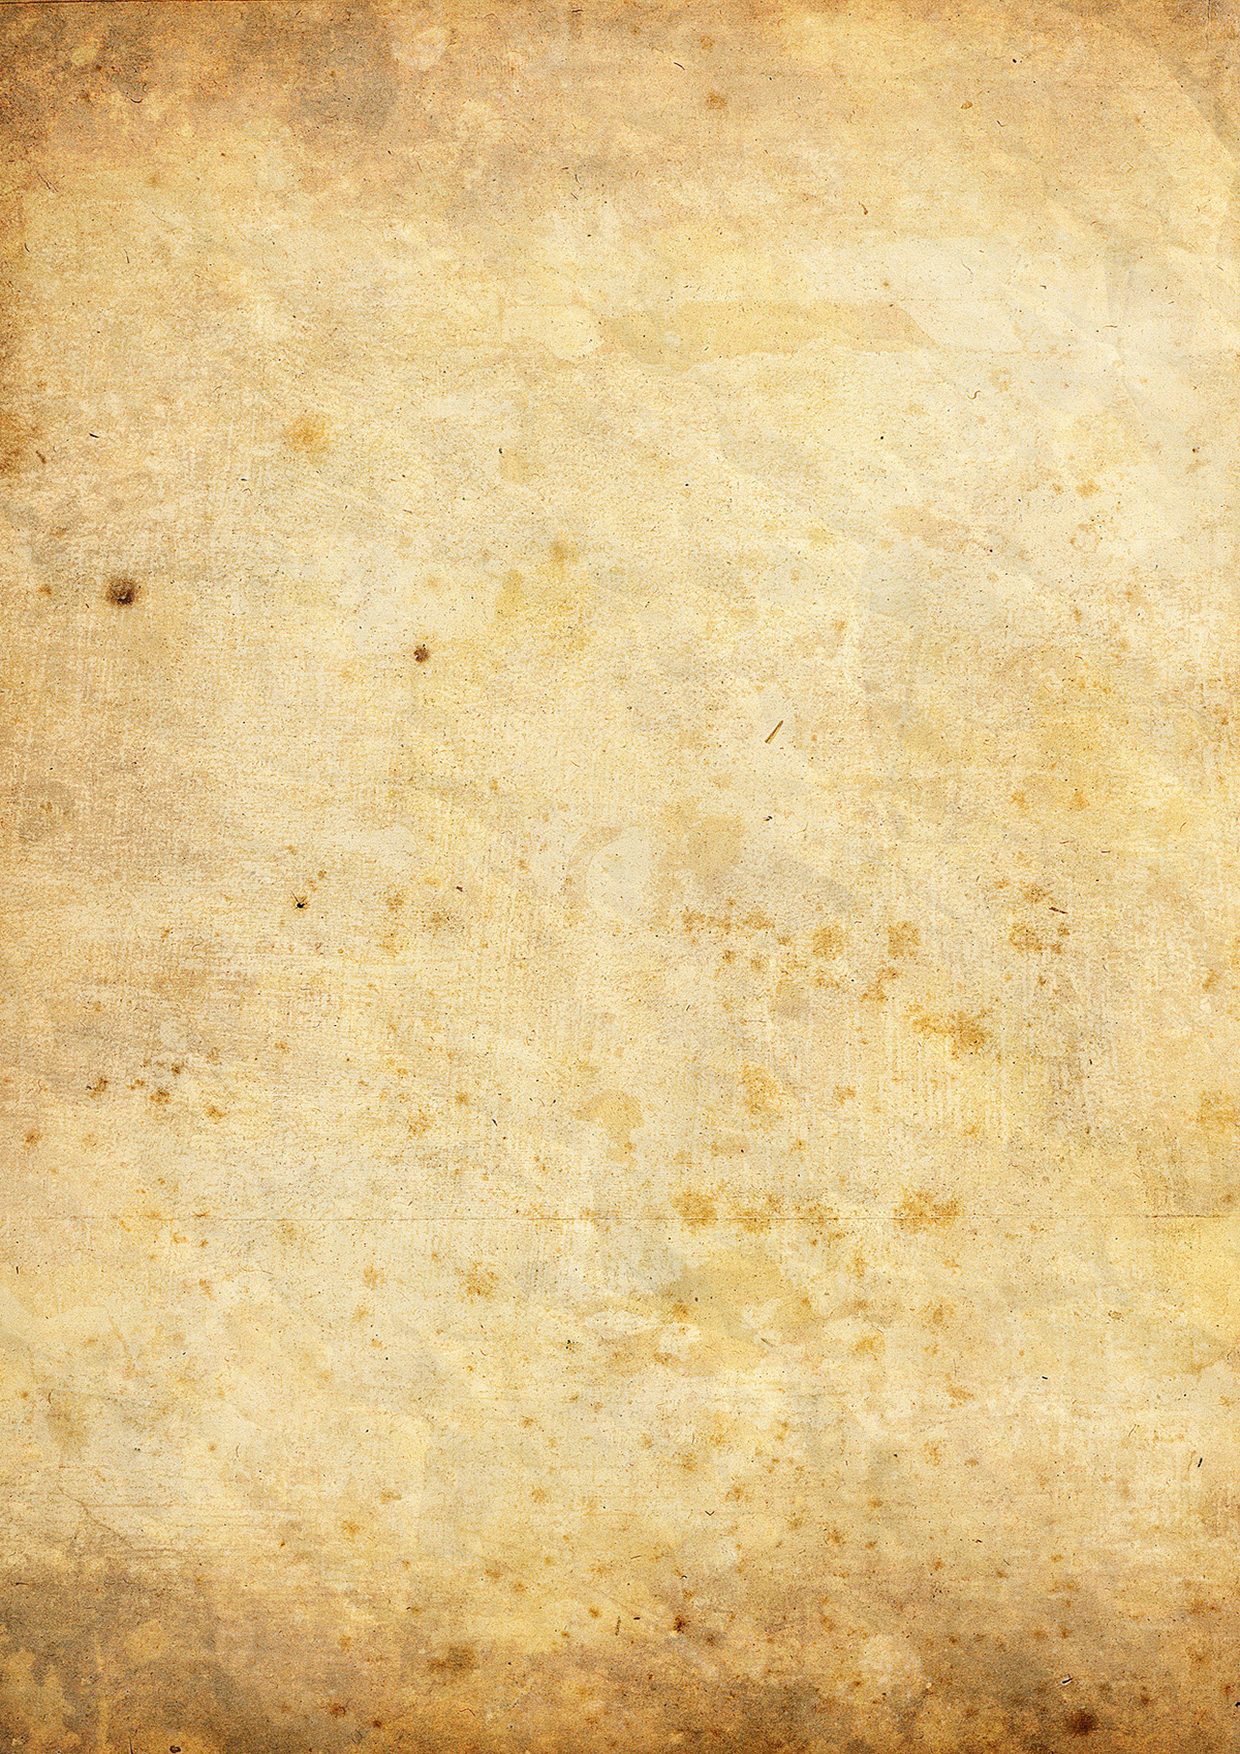
\includegraphics[width=\paperwidth,height=\paperheight,keepaspectratio]{img/final/galat/e4.jpg}%
\vfill
}}}




%\usepackage{pb-diagram}
%\newgeometry{paper=a5paper,top=12.7mm, bottom=12.7mm,left=12.7mm,right=12.7mm,bindingoffset=3mm,includefoot}
\newcommand{\mpd}{\left(\frac{M}{P}\right)^d}
\newcommand{\msp}{\left(\frac{M^s}{P}\right)}
\let\oldleadsto\leadsto
\renewcommand{\leadsto}{\hspace*{1ex plus .3ex minus .2ex}\Rightarrow\hspace*{1ex plus .3ex minus .2ex}}
\newenvironment{dano}{%
\setlength{\parskip}{0.1em plus 0.05em minus 0.05em}
  \begin{quote}
}{%
  \end{quote}
}

\usepackage[pdftex,unicode,bookmarks=true,bookmarksopen=true,colorlinks=true,linkcolor=blue,urlcolor=blue,citecolor=blue]{hyperref}
\usepackage{marvosym}
\usepackage{ulem}
\usepackage{bbm}
\usepackage{accents}
\usepackage{asymptote}
\usepackage{wasysym}
\usepackage{pdfpages}

\makeatletter
\renewcommand*\l@section[2]{
\ifnum \c@tocdepth >\z@
    \addpenalty\@secpenalty
    \addvspace{1.0em \@plus\p@}%
    \setlength\@tempdima{2em}%
    \begingroup
      \parindent \z@ \rightskip \@pnumwidth
      \parfillskip -\@pnumwidth
      \leavevmode \bfseries
      \advance\leftskip\@tempdima
      \hskip -\leftskip
      #1\nobreak\hfil \nobreak\hb@xt@\@pnumwidth{\hss #2}\par
    \endgroup
  \fi}
%\DeclareSymbolFont{largesymbolsA}{U}{pxexa}{m}{n}
%\SetSymbolFont{largesymbolsA}{bold}{U}{pxexa}{bx}{n}
%\def\re@DeclareMathSymbol#1#2#3#4{%
%    \let#1=\undefined
%    \DeclareMathSymbol{#1}{#2}{#3}{#4}}
%\re@DeclareMathSymbol{\ointctrclockwiseop}{\mathop}{largesymbolsA}{10}
%   \def\ointctrclockwise{\ointctrclockwiseop\nolimits}
\makeatother
%\usepackage{mathabx}
%\usepackage{teubner}

%
%Шаблоны

%\delimitershortfall-1pt


\renewcommand{\a}{\langle}
\newcommand{\s}{\rangle}
%\newcommand{\gom}{\mathfrak{S}}
\newcommand{\gom}{$\SpecialForty$}
\newcommand{\ol}[1]{\overline{#1}}
\newcommand{\To}[1]{\xrightarrow{#1}}
\newcommand{\tend}[1]{\xrightarrow[#1]{}}
\newcommand{\Tot}[1]{\xrightarrow{\text{#1}}}
\newcommand{\imp}{\hspace{1pt plus1pt}\Rightarrow\hspace{1pt plus1pt}}
\newcommand{\ifff}{\Leftrightarrow}
\newcommand{\Uvek}{u_1,\ldots,u_k}
\newcommand{\Avek}{a^1,\ldots,a^k}
\newcommand{\Lam}{\lambda_1,\ldots,\lambda_k}
\newcommand{\Llaa}{\lambda_1 a^1+\ldots+\lambda_k a^k}
\newcommand{\Llak}{\lambda_1 u_1+\ldots+\lambda_k u_k}
\newcommand{\Lmuk}{\mu_1 u_1+\dots+\mu_k u_k}
\newcommand{\lra}{\longrightarrow}
\newcommand{\lla}{\longleftarrow}
\newcommand{\llr}{\leftrightarrows}
\newcommand{\giraf}{\underset{f}{\overset{g}{\leftrightarrows}}}
\newcommand{\rf}{\overset{f}{\longrightarrow}}
\newcommand{\rg}{\overset{g}{\longrightarrow}}
\newcommand{\epr}{\rightsquigarrow}
\newcommand{\pos}[1]{\big\{{#1}_n\big\}_{n=1}^\infty}
\newcommand{\ar}[4]{\big\{{#1}_{#2}\big\}_{#2=#3}^{#4}}
\newcommand{\Har}[4]{\left\{{#1}_{#2}\right\}_{#2=#3}^{#4}}
\newcommand{\aR}[2]{\big\{#1\big\}_{#2=1}^{\infty}}
\newcommand{\HaR}[2]{\left\{#1\right\}_{#2=1}^{\infty}}
\newcommand{\AR}[3]{\big\{#1\big\}_{#2}^{#3}}
\newcommand{\rk}{\mathrm{rk}}
\newcommand{\nin}{\notin}
\newcommand{\nni}{\ \cancel{\ni}\ }
\newcommand{\dd}{\setminus}
\newcommand{\nuu}{\overline{\vphantom{<}\quad}\kern-.35em\searrow}
\newcommand{\nv}{\underline{\vphantom{<}\quad}\kern-.35em\nearrow}
\newcommand{\q}{\varnothing}
\renewcommand{\O}{\varnothing}
\newcommand{\N}{\mathds{N}}
\newcommand{\Q}{\mathds{Q}}
\newcommand{\R}{\mathds{R}}
\newcommand{\T}{\mathbb{T}}
\renewcommand{\C}{\mathds{C}}
\newcommand{\eH}{\mathfrak H}
\newcommand{\Z}{\mathds{Z}}
\renewcommand{\F}{\Digamma}
\newcommand{\Ri}{\mathrm{R}}
\newcommand{\Rim}{\mathcal R}
\newcommand{\ro}{\mathcal P}
%\newcommand{\de}{:\kern-.695em\lower-.38ex\hbox{.}\ }
\makeatletter
\newcommand*{\relrelbarsep}{.386ex}
\newcommand*{\relrelbar}{%
  \mathrel{%
    \mathpalette\@relrelbar\relrelbarsep
  }%
}
\newcommand*{\@relrelbar}[2]{%
  \raise#2\hbox to 0pt{$\m@th#1\relbar$\hss}%
  \lower#2\hbox{$\m@th#1\relbar$}%
}
\providecommand*{\rightrightarrowsfill@}{%
  \arrowfill@\relrelbar\relrelbar\rightrightarrows
}
\providecommand*{\leftleftarrowsfill@}{%
  \arrowfill@\leftleftarrows\relrelbar\relrelbar
}
\providecommand*{\xrightrightarrows}[2][]{%
  \ext@arrow 0359\rightrightarrowsfill@{#1}{#2}%
}
\providecommand*{\xleftleftarrows}[2][]{%
  \ext@arrow 3095\leftleftarrowsfill@{#1}{#2}%
}

\newcommand{\rsh}[2][P]{\xrightrightarrows[{#2\to\infty}]{#1}}
\newcommand{\rsH}[2][X]{\xrightrightarrows[{#2}]{#1}}
\newcommand{\nsh}[2][n]{\xrightarrow[#1\to\infty]{\|\ \|_{#2}}}

\makeatother
%\newcommand{\de}{\,\begin{sideways}\!.\,\negmedspace.\,\negmedspace.\end{sideways}\,}
\newcommand{\de}{\mathrel{\hskip.03em\vbox{\baselineskip=2.7pt\lineskiplimit=0pt\kern6pt \hbox{.}\hbox{.}\hbox{.}}\hskip.03em}}         %%%%    ???????
\newcommand{\defequiv}{\mathbin{\vbox{\baselineskip=1.95pt\lineskiplimit=0pt\hbox{.}\hbox{.}\hbox{.}}\hskip-0.3em\equiv}}
%\newcommand{\de}{\maya{3}}
%\newcommand{\de}{:\kern-.695em{\cdot}\ }
\newcommand{\pre}[3]{\lim\limits_{#2\to\infty}{#1}_{#2}=#3}
\newcommand{\pr}[2]{\lim\limits_{#2\to\infty}{#1}}
\newcommand{\oo}{\ol{\ol o}}
\newcommand{\ou}{\underline{\underline{O}}}
\newcommand{\ouu}[2]{\underset{#2\ }{\underline{\underline{O}}(#1)}}
\newcommand{\ooo}[2]{\underset{#2\ }{\ol{\ol o}(#1)}}
\newcommand{\ooob}[2]{\underset{#2}{\ol{\ol o}\big(#1\big)}}
\newcommand{\ooog}[2]{\underset{#2}{\underline{\underline O}\big(#1\big)}}
\newcommand{\te}[1][]{\xrightarrow[n\to\infty]{#1}}
\newcommand{\TE}{\xrightarrow[N\to\infty]{}}
\newcommand{\db}[3]{\underset{\substack{#2\\#3}}{#1}}
\newcommand{\dt}[4]{\underset{\substack{#2\\#3\\#4}}{#1}}
\newcommand{\dts}[4]{\underset{\substack{#2\\#3\\#4}}{#1}}
\newcommand{\ub}[3]{\overset{\substack{#3\\#2}}{#1}}
\newcommand{\tud}[2]{\underset{\substack{\downarrow\\#2}}{#1}}
\newcommand{\lims}[3]{\underset{\substack{#2\\#3}}{#1}}
\newcommand{\ums}[3]{\overset{\substack{#2\\#3}}{#1}}
\newcommand{\gf}[1]{g\big(f(#1)\big)}
\newcommand{\fg}[1]{f\big(g(#1)\big)}
\newcommand{\kom}[3]{#1\big(#2(#3)\big)}
\newcommand{\pzp}[2]{\left(1+\dfrac1{#1}\right)^{#2}}

\newcommand{\yo}[2]{\lim\limits_{#1\to#2}}
\newcommand{\prb}[2]{\lim\limits_{#2}#1}

\newcommand{\pz}[2]{\left(1+#1\right)^{\frac1{#2}}}
\newcommand{\pyd}[2]{\lim\limits_{\Delta#2\to0}\dfrac{#1({#2}_0+\Delta#2)-#1({#2}_0)}{\Delta#2}}
\newcommand{\pydo}[3]{\lim\limits_{\Delta#2\to0#3}\dfrac{#1({#2}_0+\Delta#2)-#1({#2}_0)}{\Delta#2}}
\newcommand{\py}[2]{\lim\limits_{#2\to{#2}_0}\dfrac{#1(#2)-#1({#2}_0)}{#2-{#2}_0}}
\newcommand{\pyo}[3]{\lim\limits_{#2\to{#2}_0#3}\dfrac{#1(#2)-#1({#2}_0)}{#2-{#2}_0}}
\newcommand{\tab}[2]{\begin{tabular}{#1}#2\end{tabular}}
\newcommand{\pic}[4]{\begin{figure}[htbp]\centering\includegraphics[height=#2cm]{img/final/#1.pdf}\caption{#4}\label{#3}\end{figure}}
\newcommand{\Pic}[4]{\begin{figure}[H]\centering\includegraphics[height=#2cm]{img/final/#1.pdf}\caption{#4}\label{#3}\end{figure}}
%\newcommand{\npic}[4]{\begin{figure}[htbp]\centering\includegraphics[height=#2cm]{img/final/#1.pdf}&\includegraphics[height=#2cm]{img/final/#1.pdf}\caption{#4}\label{#3}\end{figure}}
\newcommand{\ma}[1]{\begin{matrix}#1\end{matrix}}
\newcommand{\z}{\downarrow}
\newcommand{\pn}[5]{\sum\limits_{k=#3}^{#4}\dfrac{{#1}^{(k)}(#5)}{k!}(#2-#5)^k}

\newcommand{\rus}[1]{\mbox{\rm{\scriptsize{#1}}}}
\newcommand{\pau}{\hskip .75em plus.1em minus.08em\relax}

\newcommand{\tire}{"---}
\newcommand{\sdc}{a_{11}x^2+2a_{12}xy+a_{22}y^2+2a_1x+2a_2y+a_0}
\newcommand{\Sdc}[1]{a_{11}x_{#1}^2+2a_{12}x_{#1}y_{#1}+a_{22}y_{#1}^2+2a_1x_{#1}+2a_2y_{#1}+a_0}
%?????????
% Асимптота!!!!!!!!!!!!!!!!!!!!!

\newcommand{\inz}{\bowtie}

%???????:
\newcommand{\VEC}[1]{\overrightarrow{#1}}
\newcommand{\mn}[4]{#1(#2)={#3}_{#4}{#2}^{#4}+\ldots+{#3}_0}
\newcommand{\Mn}[4]{#1(#2)={#3}_{#4}{#2}^{#4}+{#3}_{#4-1}{#2}^{#4-1}\ldots+{#3}_{1}{#2}+{#3}_0}

\newcommand{\tp}{точная первообразная}
\newcommand{\op}{обобщённая первообразная}
\newcommand{\oP}{\int\limits_0^{\pi}}
\newcommand{\mpP}{\int\limits_{-\pi}^{\pi}}
\newcommand{\ds}{\displaystyle}
\newcommand{\Cn}[2]{\overset{#2}{\cancel{#1}}}
\newcommand{\ve}[2]{(#1_1,\ldots,#1_{#2} )} % \ve xn |---> (x_1,\ldots, x_n)
\newcommand{\vem}[3]{(#1_1,\ldots,#1_{#2},\ldots,#1_{#3} )}
\newcommand{\vef}[3]{#1_1#2,\ldots,#1_{#3}{#2} }
\newcommand{\Til}[1]{\widetilde{#1}{} }
\newcommand{\TTil}[1]{\widetilde{\widetilde{#1}}{} }
\newcommand{\D}[1]{\overline{\Delta #1}}
\newcommand{\CP}[2]{\frac{\partial #1}{\partial #2}}
\newcommand{\Jacoby}[4]{\begin{pmatrix}
\CP {{#1}_{1}}{{#2}_1} 	& \CP{{#1}_{1}}{{#2}_2} & \dots & \CP{{#1}_{1}}{{#2}_{#3}} \\[1ex]
\CP {{#1}_{2}}{{#2}_1} 	& \CP{{#1}_{2}}{{#2}_2} & \dots & \CP{{#1}_{2}}{{#2}_{#3}} \\
\vdots 			& \vdots		& \ddots& \vdots \\
\CP {{#1}_{#4}}{{#2}_1} & \CP{{#1}_{#4}}{{#2}_2}& \dots & \CP{{#1}_{#4}}{{#2}_{#3}}
\end{pmatrix}}
\newcommand{\jacoby}[4]{\begin{pmatrix}
\CP {{#1}_{1}}{{#2}_1} 	& \dots & \CP{{#1}_{1}}{{#2}_#3} & \CP{{#1}_{1}}{{#2}_{#3+1}} \\
\vdots 			& \ddots& \vdots		 & \vdots \\
\CP {{#1}_{#4}}{{#2}_1} & \dots & \CP{{#1}_{#4}}{{#2}_#3}& \CP{{#1}_{#4}}{{#2}_{#3+1}} \\[1ex]
\CP {{#1}_{#4+1}}{{#2}_1} & \dots & \CP{{#1}_{#4+1}}{{#2}_#3}& \CP{{#1}_{#4+1}}{{#2}_{#3+1}}
\end{pmatrix}}

\newcounter{rad}
\setcounter{rad}{1}
% a_1+a_2+\ldots
	\def\rad#1#2{\ifnum \therad < \the\numexpr(#2 + 1)\relax #1_\therad + \addtocounter{rad}{1} \rad{#1}{#2}\else \ldots \fi \setcounter{rad}{1}}
%a_{N+1}+a_{N+2}+\ldots
	\def\raD#1#2#3{\ifnum \therad < \the\numexpr(#2 + 1)\relax #1_{#3{\therad}} + \addtocounter{rad}{1} \raD{#1}{#2}{#3}\else \ldots \fi \setcounter{rad}{1}}

\newcommand{\ry}[3][1]{\sum\limits_{{#3}={#1}}^\infty {#2}_{#3}}
\newcommand{\rY}[2][1]{\sum\limits_{{#2}={#1}}^\infty}
\newcommand{\RY}[3]{\sum\limits_{#1 = #2}^{#3}}
%\left(\frac11\right)^2+\left(\frac12\right)^2+\left(\frac13\right)^2+\ldots+\left(\frac1{N+1}\right)^2
	\def\crad#1#2#3#4{\ifnum \therad < \the\numexpr(#4 + 1)\relax #1{\therad}#3 + \addtocounter{rad}{1} \crad{#1}{#2}{#3}{#4}\else \ldots +#1{#2}#3 \fi \setcounter{rad}{1}}
%\left(\frac1{n+1-j}\right)^2+\left(\frac1{n+2-j}\right)^2+\left(\frac1{n+3-j}\right)^2+\ldots+\left(\frac1{n+N+1-j}\right)^2
	\def\craD#1#2#3#4#5#6{\ifnum \therad < \the\numexpr(#4 + 1)\relax #1{#5{\therad}#6}#3 + \addtocounter{rad}{1} \craD{#1}{#2}{#3}{#4}{#5}{#6}\else \ldots +#1{#5#2#6}#3  \fi \setcounter{rad}{1}}
%repeat argument #1 #2 times
	\def\tfT#1#2{\ifnum \therad < \the\numexpr(#2 + 1)\relax #1\addtocounter{rad}{1} \tfT{#1}{#2}\else \fi \setcounter{rad}{1}}

\newcommand{\aee}[1][\varepsilon > 0]{\forall\ #1\pau \exists\ }
%a_1\le a_2\le a_3\le \ldots\le a_n
	\def\dI#1#2#3#4#5#6{\ifnum \therad < \the\numexpr(#6 + 1)\relax {#1}_{\therad}{#3}_{\therad}#5\addtocounter{rad}{1} \dI{#1}{#2}{#3}{#4}{#5}{#6}\else \dots #5{#1}_{#2}{#3}_{#4}\fi \setcounter{rad}{1}}
%x^1y_1\otimes x^2y_2 \otimes x^3y_3 \otimes \dots \otimes x^ky_k
	\def\DI#1#2#3#4#5#6{\ifnum \therad < \the\numexpr(#6 + 1)\relax #1\therad#3\therad#5\addtocounter{rad}{1} \DI{#1}{#2}{#3}{#4}{#5}{#6}\else \dots #5#1#2#3#4\fi \setcounter{rad}{1}}
%192-1 туфли классические пакет с классическими брюками

%a_1b_3+a_2b_2+a_3b_1
\def\iSum#1#2#3{\ifnum \therad < #3\relax {#1}_{\therad}{#2}_{\the\numexpr(#3 - \therad + 1)\relax}+ \addtocounter{rad}{1}\iSum{#1}{#2}{#3}\else {#1}_{\therad}{#2}_{1}\fi \setcounter{rad}{1}}

\def\tms#1#2{\ifnum \therad < \the\numexpr(#2 + 1)\relax #1_\therad \ifnum \therad < \the\numexpr(#2)\relax \cdot \else \fi\addtocounter{rad}{1} \tms{#1}{#2}\else \cdots \fi \setcounter{rad}{1}}
\def\ctms#1#2#3#4#5{\ifnum \therad < \the\numexpr(#4 + 1)\relax #1{#2\therad}#3 \ifnum \therad < \the\numexpr(#4)\relax \cdot \else \fi\addtocounter{rad}{1} \ctms{#1}{#2}{#3}{#4}{#5}\else \cdots #1{#2#5}#3\fi \setcounter{rad}{1}}
\newcommand{\tmy}[2]{\prod\limits_{#2=1}^{\infty}#1_{#2}}
\newcommand{\tmY}[1]{\prod\limits_{#1=1}^{\infty}}
\newcommand{\tMY}[2][n]{\prod\limits_{#1=#2}^{\infty}}

\newcommand{\podP}[5][\infty]{\big\{{#2}_{{#3}_{#4}}\big\}_{#4=#5}^{#1}}
\newcommand{\poDP}[4][\infty]{\big\{{#2}_{{#3}_{#4}}\big\}_{#4=1}^{#1}}
\DeclareMathOperator{\diam}{diam}
\DeclareMathOperator{\card}{card}
\DeclareMathOperator{\osc}{osc}
\DeclareMathOperator{\grad}{grad}
\DeclareMathOperator{\intS}{int}
\DeclareMathOperator{\ext}{ext}
\DeclareMathOperator{\rot}{rot}
\DeclareMathOperator{\cur}{cur}
\DeclareMathOperator{\divergence}{div}
\renewcommand{\Re}{\mathop{\text{Re}}}
\renewcommand{\Im}{\mathop{\text{Im}}}
\newcommand{\bou}[1]{\partial #1}
\newcommand{\mea}[1]{\mu #1}
\newcommand{\Mea}[1]{\mu \left(#1\right)}


\newenvironment{iItems}{\begin{enumerate}\let\AEtheenumi\theenumi{}\renewcommand{\theenumi}{\roman{enumi}}\renewcommand{\labelenumi}{(\theenumi)}}{\renewcommand{\labelenumi}{\theenumi.}\renewcommand{\theenumi}{\AEtheenumi}\end{enumerate}}
\newenvironment{azItems}{\begin{enumerate}\let\AEtheenumi\theenumi{}\renewcommand{\theenumi}{\asbuk{enumi}}\renewcommand{\labelenumi}{(\theenumi)}}{\renewcommand{\labelenumi}{\theenumi.}\renewcommand{\theenumi}{\AEtheenumi}\end{enumerate}}
\newenvironment{roItems}{\begin{enumerate}\renewcommand{\labelenumi}{(\theenumi)}}{\renewcommand{\labelenumi}{\theenumi.}\end{enumerate}}
\newenvironment{oItems}{\begin{roItems}\setcounter{enumi}{-1}}{\end{roItems}}

\newcommand{\iY}[1][1]{\ds\int\limits_{#1}^{\infty}}
\newcommand{\IY}[2]{\ds\int\limits_{#1}^{#2}}
\newcommand{\cSize}{\footnotesize}
\newcommand{\cmt}[1]{\text{\cSize #1}}

\newcommand{\far}[3]{\big\{#1_{#2}(#3)\big\}_{#2=1}^{\infty}}
\newcommand{\Aq}{\mathfrak A}
\newcommand{\Tau}{\mathcal T}
%\newcommand{\overcirc}[1]{\mathring{#1}}%http://tex.stackexchange.com/questions/3266/how-do-i-use-a-circle-as-a-math-accent-larger-than-mathring
\newcommand{\overcirc}[1]{\accentset{\circ}{#1}}
\newcommand{\overstar}[1]{\accentset{\bigstar}{#1}}


\newcommand{\W}{\Omega}
\newcommand{\Ax}[3][]{#1 #2_{\ol #3}}
\newcommand{\Kprod}{\wedge}
\newcommand{\KP}{\Kprod}
\newcommand{\lom}{\mathrm{lom}}


%\input{coffee4.sty}

\setlength{\parskip}{1em plus 0.05em minus 0.05em}
\newtheorem{Def}{Определение}[section]
     \newtheorem{Th}{Лемма}[section]
     \newtheorem{The}{Теорема}[section]
     \newtheorem{Pre}{Предложение}[section]
     \newtheorem{Sl}{Следствие}[section]
     \newtheorem{Ut}{Утверждение}[section]
     \newenvironment{Zam}
     	{\par\noindent{\textbf{Замечание.}}}{}
     \newenvironment{Proof}
       {\par\noindent{\textbf{Доказательство.}}}
       {\hfill$\scriptstyle\blacksquare$}
\renewcommand{\thefootnote}{\fnsymbol{footnote}}
\DefineFNsymbols*{snoski}{{$\dagger$}{$\ddagger$}\S\P{$\|$}\#}
\setfnsymbol{snoski}

\let\AVsection\section{}
\renewcommand\section{\newpage\scol\AVsection}
\let\AEpart\part{}
\renewcommand\part{\newpage\bezcol\AEpart}
\setlength{\headheight}{14pt}
\setlength{\headsep}{\baselineskip}


\pagestyle{fancyplain}
\renewcommand{\sectionmark}[1]{\markboth{#1}{}}
\fancyhead{}
\fancyhead[RE,LO]{\thesection{} \leftmark}
\fancyhead[LE,RO]{\thepage}
\fancyfoot{}
\newcommand{\bezcol}{\renewcommand{\headrulewidth}{0pt}\fancyhead{}}
\newcommand{\scol}{  \renewcommand{\headrulewidth}{0.5pt}\fancyhead[RE,LO]{\thesection{} \leftmark} \fancyhead[LE,RO]{\thepage}}

\begin{document}
\bezcol
\pagestyle{empty}
\renewcommand{\thepage}{\Roman{page}}
\vspace*{2\baselineskip}
\begin{center}
{\huge Треть курса «Математический анализ»}\\[2ex]
\large\copyright~Доцент В.",В.",Галатенко (списывание с доски\footnote{%
За исключением, быть может, конечного числа лекций.} и вёрстка в \LaTeX{} "--- А.",Е.",Ширыкалов). \\[2ex]
Последнее обновление произошло \today
\end{center}

\begin{figure}[H]\centering

\includegraphics[width=30mm]{img/final/galat/main.pdf}\caption*{Ёжик уже дочитал до \ref{LEN}}
\end{figure}
\begin{abstract}
 Перед вами уже достаточно большой файл. Кому-то может показаться странным то, что файл один, а~не~хотя~бы два: по~одному на~каждый семестр.
 Через год, когда количество страниц дорастёт уже до какого-то совсем большого числа, все лекции всё ещё будут в~одном файле. Это важно.
 
 В центре внимания "--- гиперссылки. Оглавление полностью интерактивное, то~есть одним кликом вы оказываетесь там, где хотите быть.
 Оно находится в~начале, что очень полезно для обладателей устройств, на~которых неудобно листать страницы.
 Что совсем в центре внимания: гиперссылки конкретно в доказательствах.
 Для них как раз и нужно сохранять лекции с первого семестра.
 Хорошим студентам, конечно, не нужно напоминать, что такое теорема \ref{Lag} Лагранжа, но
 возможность её мгновенно найти делает всех студентов хорошими, когда в руках этот документ.
 Есть программы для просмотра файлов PDF, в~которых после того, как вы прошли по~ссылке в~какую-то
 часть файла, можно с~помощью клавиши «Backspace» моментально вернуться назад.
 Если вы вдруг ещё работаете с~системой Windows, то~такую~возможность вам предоставит
 \href{http://blog.kowalczyk.info/software/sumatrapdf/free-pdf-reader.html}{Sumatra PDF}. Можно даже будет
 чуть-чуть «скроллить» перед тем, как нажать «Backspace».
 
 Кроме того этот файл стремится к тому, чтобы быть образцом хорошей типографики. Не очень быстро, но~стремится.
 Русская традиция тонких пробелов вокруг знака тире, свешивающаяся пунктуация, точки над буквой ё, перенос знаков равенства, тонкие
 пробелы перед $dx$ в интегральных выражениях и многое другое "--- школа \href{http://kostyrka.ru/blog/}{Андрея Викторовича Костырки}.
  \end{abstract}

\newpage
%\AddToShipoutPicture{\bgpic}
\tableofcontents

\newpage\renewcommand{\thepage}{\arabic{page}}\setcounter{page}{1}
  
    
    \part{Первый осенний семестр}
    
    \pagestyle{fancyplain}  
\section{Множества и операции над~множествами}
\subsection{Чёрный ящик отвечает на~вопросы}

Определить "--- описать в~терминах уже определённых понятий, спуститься на~ступеньку вниз.
А множество есть неопределяемое понятие, просто потому, что всегда настанет ситуация, когда ниже некуда опускаться.
 Должно быть такое понятие, через которое будем определять все остальные. Поэтому для множества вводим \textbf{синонимическое описание}:

Множество "--- это совокупность (набор, семейство) некоторых агентов (объектов "--- элементов множества).
Основное действие по~множеству и элементу: проверить, принадлежит ли этот объект этому множеству.

Обозначения того, что элемент $a$ принадлежит  множеству $A$ или, что равносильно,
$A$ содержит $a$:
    $a\in A\hm{\iff} A \ni a$.
И не принадлежит и не содержит:
  $a\notin  A\hm{\iff} A \not\ni  a$.


\subsubsection{Способы задать множество}
\begin{enumerate}
    \item Перечислить все элементы: $\{0,1,2\} \hm= \{0,1,2,0\}$ "--- обратим внимание на~то, что множество "--- это некий чёрный ящик, который отвечает на~вопросы «есть ли в~тебе такой элемент?», поэтому перечисление одного элемента дважды, трижды, миллионажды никак не влияет на~число элементов множества;

    \item Задать характеристическим свойством элементов множества:

    $\{ \text{Люди}\colon \text{рост}\hm>175~\text{см}\}$.\pau Иногда вместо «:» ставят «|»;

    $\{ \text{Присутствующие студенты}\colon \overset{\text{группа крови I}}{\text{{\sout{доживут до\ldots}}}}\}$;

    $\{ \text{Действительные числа}\colon \text{в десятичной записи на~$10^9$-м месте после запятой стоит 7}\}$ "--- свойство не должно быть обязательно легко проверяемо.

     \end{enumerate}
    
    $\varnothing$ "--- множество, которое не содержит элементов. Чёрный ящик ушёл в~\textit{отрицанку}.

    $\{\varnothing\},\big\{\{\varnothing\}\big\}$ "--- вовсе не пустые множества.
    Ну вот начал человек собирать марки, купил альбом. Марок нет, а~альбом есть, есть полка под~альбомы.

    Нет понятия \textbf{множество, которое содержит всё}.

    \textbf{Парадокс Рассела:} множество всех объектов невозможно.

    Рассмотрим совокупность всех множеств $A$, которые не содержат себя в~качестве элемента ($A\notin A$). Обозначим совокупность через $B$.

    $A\in B \hm{\iff} A\notin A$, верно ли, что $B$ является элементом себя?

    $B\in B \hm{\iff} B\notin B$ "--- противоречие, такая вот неудача. \textbf{Неопределяемые множества рождают парадоксы.}

    Парадокс брадобрея: бреет бороды всем, кто сам себя не бреет, бреет ли брадобрей себя?

    Не существует чёрного ящика, который всегда отвечает да.


\subsubsection{Что у множества можно спросить}

Проверить, есть ли в~множестве элементы? Если есть, то в~множестве можно найти элемент, принадлежащий множеству.

Пусть $A$ и $B$ "--- какие-то множества.

\begin{Def}
    Объединением $A$ и $B$  ($A\cup B$) или ($A+B$) называют множество, состоящее из~тех и только тех элементов, которые входят хоть в~одно из~множеств $A$ и $B$.
\end{Def}

А у множества можно спрашивать: \textit{в тебя входят?}

\pic{galat/1/unite}{1.5}{unite}{Объединение множеств}

\begin{Def}
    Пересечение множеств $A$ и $B$  ($A\cap B$) "--- это множество, состоящее из~тех и только тех элементов, которые входят одновременно и в~$A$, и в~$B$.
\pic{galat/1/cross}{1.5}{cross}{Пересечение множеств}
\end{Def}

\begin{Def}
    Разность множеств $A$ и $B$ ($A\dd B$) "--- множество, состоящее из~тех и только тех элементов, для которых верно: $a\in A$, но $a\notin B$.
\pic{galat/1/minus}{1.5}{minus}{Разность множеств}


\end{Def}


    Симметрическая разность множеств $A$ и $B$ ($A\triangle B$) "--- множество, состоящее из~тех и только тех элементов,
     которые входят ровно в~одно множество $A$ или $B$.
    %\pic{galat/1/simraz}{1.5}{simraz}{Симметрическая разность}
    $$    A\triangle B\hm=(A\dd B)\cup (B\dd A).   $$



\begin{Def}
    Множество $A$ является подмножеством множества $B$ ($A\subset B, B \supset A$), если любой элемент $A$ является элементом $B$.
\end{Def}

\begin{Def}
    Множества $A$ и $B$ совпадают ($A\hm=B$), если они состоят из~одних и тех же элементов.
        $$A\hm=B\ \hm{\iff}\ A\subset B,B\subset A.$$
\end{Def}

$A\cup B\hm=B\cup A,\pau A\cap B\hm=B\cap A$ "--- коммутативность;

$(A\cup B)\cup C\hm=A\cup (B\cup C),\pau(A\cap B)\cap C\hm=A\cap (B\cap C)$ "--- ассоциативность;

$(A\cup B)\cap C\hm=(A\cap C)\cup(B\cap C)$ "--- дистрибутивность;

$A\cup \varnothing\hm=A,\qquad A\cup A\hm=A$;

$A\cap \varnothing\hm=\varnothing\qquad A\cap A\hm=A$;

$(A\dd B)\cup B\hm=A\cup B$.

\begin{Pre}[Принцип Моргана]\label{PM} $A\dd(B\cup C)\hm=(A\dd B)\cap (A\dd C)$.


    $A\dd(B\cap C)\hm=(A\dd B)\cup (A\dd C)$ "--- двойственность.
\end{Pre}
\section{Совокупности множеств и пары}

Не стоит путать значки: $b\in A, \ B\subset A$ "--- проще оценить разницу, когда
 $\varnothing\notin\{1\},\ \varnothing\subset A$, если $A$ "--- любое множество.

$A\subset A$;

Если $A\subset B,\ B\subset C$, то $A\subset C$ "--- транзитивность (глубоко научное слово).

Тривиальные множества: $\{1\}\ \{2\}$ "--- ни одно из~них, не входит в~другое.

$A\subseteq B$ "--- в~старой литературе. Здесь в~наше $\subset$ вложена возможность быть равным.

$A\varsubsetneq B$ "--- редко будем писать.
\subsection{Правила Моргана}
Вспомним правила Моргана (\ref{PM}).

\begin{Proof}
    \begin{enumerate}
        \item \label{q}Пусть $a \in A\dd(B\cap C)$, тогда $a\in A,\ a\notin(B\cap C)$, то есть $a\notin B \cup a\notin C$;

            Если $a\notin B$, то $a\in (A\dd B)$, а~значит $a\in(A\dd B) \cup (A\dd C)$;

            Если $a\notin C$, то $a\in(A\dd C)$, а~значит $a\in (A\dd C)\cup (A\dd B)$;

            То есть $A\dd (B\cap C)\subset (A\dd B)\cup (A\dd C)$;

        \item\label{w} Пусть $a\in (A\dd B)\cup (A\dd C)$;

        $a\in (A\dd B)\cup a\in (A\dd C)$;

        Если $a\in (A\dd B) \hm{\imp} (a\in A)\cap (a\notin B)$, тогда $a\notin (B\cap C) \hm{\imp} a\in A\dd(B\cap C)$;

        Если $a\in (A\dd C) \hm{\imp} (a\in A)\cap (a\notin C)$, тогда $a\notin (B\cap C) \hm{\imp} a\in A\dd(B\cap C)$;

        $A\dd (B\cap C)\supset (A\dd B)\cup (A\dd C)$;

        из~пунктов \ref{q} и \ref{w} следует, что  $A\dd(B\cap C)\hm=A\dd B\cup A\dd C$.

    \end{enumerate}
\end{Proof}

Как бы это компактно сократить.

Пусть $A\subset X$.
\begin{Def}
    Дополнением $A$ (относительно $X$) называется $X\dd A$.
\end{Def}

    Обозначений много, например $A^*$.

    \begin{Sl}(из \ref{PM})
        Если $B,C\subset X$, то

        \begin{enumerate}
            \item $(B\cup C)^*\hm=B^*\cap C^*$;

            \item $(B\cap C)^*\hm=B^*\cup C^*$.
        \end{enumerate}
    \end{Sl}

Пусть $M$ "--- произвольная совокупность множеств.

\begin{Def}
    Объединением совокупности множеств $M$ называется множество, состоящее из~тех и только тех элементов,
     которые являются элементами хотя бы одного множества из~совокупности $M$.
\end{Def}

\begin{Def}
     Пересечением совокупности множеств $M$ называется множество, состоящее из~тех и только
      тех элементов, которые входят во все множества из~совокупности $M$.
\end{Def}

$\bigcup\limits_{A\in M} A,\pau \bigcap\limits_{A\in M} A$ "--- так редко пишут и редко говорят.

$A_y\hm=\{x$ "--- числа: $\sin x\hm=y\}$;

$B_x\hm=(x-1,x+1)$;

$\{A_\gamma\}_{\gamma\in \Gamma}$ "--- множество всех $A_{\gamma}$, где гамма пробегает гамма большое.

Обозначение $\bigcup\limits_{\gamma\in \Gamma} A_{\gamma},\pau
\bigcap\limits_{\gamma\in \Gamma} A_{\gamma}$.

\begin{Def}
$\bigcup\limits_{\gamma\in \Gamma} A_{\gamma}$ "--- совокупность тех и только тех элементов,
 которые входят в~$A_\gamma$ хоть для одного $\gamma\in\Gamma$.
\end{Def}


\begin{Def}
$\bigcap\limits_{\gamma\in \Gamma} A_{\gamma}$ "--- совокупность тех и только тех элементов,
 которые входят в~$A_\gamma$ для всех $\gamma\in\Gamma$.
\end{Def}

\textbf{Кванторы}

$\forall$ "--- «для любого» "--- классики так его называют;

$\exists$ "--- «существует».

Иногда $\exists!$ "--- «существует и единственный».

$\forall$ человека $\exists$ число: это число является номером его паспорта. 

Порядок очень важен.

Отрицание: $\forall \lra \exists$, $\exists\lra\forall$, последнее утверждение наоборот. То есть: существует (хотя бы один) человек, для которого любое число не~является номером его паспорта.
И формальнее: $\exists$ человек: $\forall$ число не является номером его паспорта.

$A\subset B \hm{\iff} \forall\  a\in A\pau a\in B$;

$A\not\subset B \hm{\iff} \exists\  a\in A\colon a\notin B$;

$\bigcup\limits_{A\in M} A\hm=\{x\colon \exists\  A\in M\colon x\in A\}$;

$\bigcap\limits_{A\in M} A\hm=\{x\colon \forall\  A\in M\colon x\in A\}$;

$\bigcup\limits_{{\gamma\in \Gamma}} A_{\gamma}\hm=\{x\colon \exists\  \gamma\in\Gamma\colon x\in A_\gamma\}$;


$\begin{matrix}
(1)&\forall\  a\in A&\ldots\\
(2)& \exists\  a\in A&\ldots \\
\end{matrix}$ \qquad из~(1) следует (2), если $A\neq \q$.

Для $\forall\  a\in \q$ верно всё что угодно, ибо отрицание к~такому утверждению есть $\exists$ элемент $a\in\q$, который не удовлетворяет\ldotst{}


        \begin{Ut} $\left(\bigcup\limits_{\gamma\in \Gamma} A_\gamma\right)\bigcap
            \left(\bigcup\limits_{\mu\in M} A_\mu\right)\hm=\bigcup\limits_{\substack{\gamma\in \Gamma \\ \mu\in M}} \left(A_\gamma\cap B_\mu\right)$.
        \end{Ut}
        \begin{Ut} $\left(\bigcap\limits_{\gamma\in \Gamma} A_\gamma\right)\bigcup
            \left(\bigcap\limits_{\mu\in M} A_\mu\right)\hm=\bigcap\limits_{\substack{\gamma\in \Gamma \\ \mu\in M}} \left(A_\gamma\cup B_\mu\right)$.
        \end{Ut}

            $\exists\  \gamma\in\Gamma,\ \exists\ \mu\in M\colon a\in(A_\gamma\cap B_\mu)$ "--- доказывать в~обе стороны! Если влево, то вправо, если вправо, то влево. Или иначе: если влево, то вправо, и если не влево, то не вправо.

        Ещё парочка утверждений.

        \begin{Ut}\label{tri}
            $A\dd\left(\bigcup\limits_{\gamma\in\Gamma} B_\gamma\right)\hm=
            \bigcap\limits_{\gamma\in\Gamma} \left(A\dd B_\gamma\right)$.
        \end{Ut}


        \begin{Ut}
            $A\dd\left(\bigcap\limits_{\gamma\in\Gamma} B_\gamma\right)\hm=
            \bigcup\limits_{\gamma\in\Gamma} \left(A\dd B_\gamma\right)$.
        \end{Ut}

        \begin{Sl}\label{Themor}
            Из~последних пунктов: если $B_\gamma\subset X, \pau X^*$ "--- дополнение относительно X, то $
            \left(\bigcup\limits_{\gamma\in\Gamma}B_\gamma\right)^*\hm=
            \left(\bigcap\limits_{\gamma\in\Gamma}B_\gamma^*\right)$, а
            $\left(\bigcap\limits_{\gamma\in\Gamma} B_\gamma\right)^*\hm=
            \left(\bigcup\limits_{\gamma\in\Gamma}B_\gamma^*\right)$.
        \end{Sl}

        \begin{Proof} Доказываем \ref{tri}. Пусть $a\in\left(A\dd
        \bigcup\limits_{\gamma\in\Gamma} B_\gamma\right)$, то есть $\begin{cases}
            a\in A;\vphantom{\bigcup\limits_{\gamma\in\Gamma}B_\gamma} \\
            a\nin \bigcup\limits_{\gamma\in\Gamma}B_\gamma.
        \end{cases}$

    Другими словами, $\forall\  \gamma\in\Gamma\pau a\nin B_\gamma$, тогда $\forall\ \gamma\in\Gamma\pau a\in A\dd B_\gamma\hm{\imp} a\in \bigcap\limits_{\gamma\in\Gamma}(A\dd B_\gamma)$;

    В~другую сторону. Пусть $a\in\bigcap\limits_{\gamma\in\Gamma}(A\dd B_\gamma)$, тогда $\forall\  \gamma\in \Gamma\pau a\in A\dd B_\gamma$, то есть $a\in A$ и $a\nin B_\gamma$. Отсюда $a\nin \bigcup\limits_{\gamma\in\Gamma}B_\gamma$, $a\in A\dd \bigcup\limits_{\gamma\in\Gamma}B_\gamma$.
        \end{Proof}

\subsection{Что делать с~понятием функции} Если сделать базовым, то это будет грустно: давайте тогда всё будем делать базовым.
 Можно ещё жульничать через отображения. А~мы вот каким путём пойдём:

\begin{Def}
    Множество $A$ состоит из~одного элемента, если

    \begin{enumerate}
        \item $A\neq\q$;
        \item $\forall\  a\in A\colon A\dd \{a\}\hm=\q$\pau (тут можно $\forall$ поменять на~$\exists$).
    \end{enumerate}
\end{Def}

\begin{Def}
    Множество $A$ состоит из~двух элементов, если

    \begin{enumerate}
        \item $A\neq\q$;

        \item $\forall\  a\in A\colon A\dd \{a\}$ состоит из~одного элемента.
    \end{enumerate}
\end{Def}

\begin{Def}A. Неупорядоченной парой называется множество, состоящее из~двух элементов или одного элемента.

\end{Def}

\begin{Def}Б. Неупорядоченной парой элементов $a,b$ называется множество $\{a,b\}$.
\end{Def}

\textbf{Плохой пример:} (упорядоченной пары) $\{a,1\},\{b,2\}$.

\begin{Def}
    Упорядоченной парой $(a,b)$ ($a$ "--- первый элемент, $b$ "--- второй) называется $\big\{a,\{a,b\}\big\}$.
\end{Def}

\begin{Def}
    Декартовым произведением множеств $A$ и $B$ называется множество всевозможных упорядоченных пар $(a,b)$, где $a\in A,b\in B$.

    \[
        A\times B\hm=\big\{(a,b)\colon a\in A,b\in B\big\};
    \]

    \[
        A\times A\hm=A^2.
    \]
\end{Def}

$\{1\}\times\{a,b\}\hm=\big\{(1,a),(1,b)\big\}$ "--- декартово произведение не коммутативно.

\subsubsection{Свойство декартова произведения}

\[
    (A_1\cup A_2)\times B\hm=(A_1\times B)\cup(A_2\times B);
\]

\[
    (A_1\cap A_2)\times B\hm=(A_1\times B)\cap(A_2\times B);
\]

\section{Отношения}
\begin{Def}
    Отношением элементов (между элементами) множества $A$ и множества $B$ называют произвольное подмножество $A\times B$.

    Обозначим отношение $\mathcal R\pau (\mathcal R\subset A\times B)$.

    $(a,b)\in \mathcal R$\qquad $a\mathcal Rb$ "--- между элементами $a$ и $b$ есть отношение $\mathcal R$.
\end{Def}

$A$ "--- множество собравшихся людей, $B$ "--- множество букв. $a\mathcal Rb$, если буква $b$ входит в~фамилию человека $a$.

Важный случай, когда $A\hm=B$.

\begin{Def}
    Отношением на~множестве $A$ называется отношение между элементами множества $A$ и его же элементами. $(\mathcal R\subset A^2)$, где $A^2$ "--- декартов квадрат.
\end{Def}

Отношение равенства. $(a,b)\in \mathcal R \hm{\iff} a,b$ совпадают. $a\overset{\hm=}{\cancel{\mathcal R}}b$.

\begin{Def}\label{op}
    Отношение $\mathcal R$ на~множестве $A$ называется отношением порядка, если

    \begin{itemize}
        \item[0.] \label{0}$\forall\  a,b\in A\pau a\mathcal Rb$ или $b\mathcal Ra$;

        \item[1.] $(a\mathcal Rb$ и $b\mathcal Ra)\hm{\imp} a$ совпадает с~$b$;

        \item[2.] $a\mathcal Rb,b\mathcal Rc   \hm{\imp} a\mathcal Rc$.
    \end{itemize}

\end{Def}

        (А вообще этот вопрос по-разному ставится).
\begin{Def}
    Без условия 0 из определения \ref{0} "--- отношение частичного порядка.
\end{Def}

Очень важное определение:

\begin{Def}\label{deffunc}
    Отображением множества $A$ в~множество $B$ (функцией из~множества $A$ в~$B$) называется такое отношение 
    ($\mathcal R$) элементов $A$ и $B$, что $\forall\  a\in A\ \exists!\ b\in B\colon(a,b)\in \mathcal R\colon b\hm=f(a)$.
\end{Def}

\begin{Def}
    Отображение $f\colon A\to B$ ($A$ в~$B$) называется инъективным, если из~$f(a_1)\hm=f(a_2)$ следует, что $a_1\hm=a_2$
    (то есть разные элементы в~разные элементы: $a_1\neq a_2\hm{\imp} f(a_1)\neq f(a_2)$).
\end{Def}

\begin{Def}
    Отображение $f\colon A\to B$ называется сюръективным ($A$ на~$B$), если 
    \[\forall\  b\in B\ \exists\ \ a\in A\colon b\hm=f(a).\]
\end{Def}

\begin{Def}
    Отображение $f\colon A\to B$ называется биекцией (взаимно однозначным), если
    \[
        \forall\  b\in B\ \exists!a\in A\colon b\hm=f(a).
    \]
\end{Def}

\begin{Ut}
    $f$ "--- биекция $\hm{\iff}$ $f$ "--- инъекция и сюръекция одновременно.
\end{Ut}

Является ли $f(x)\hm=x^2$ биекцией, сюръекцией, инъекцией? Вопрос бессмысленный без указания множества.

Пусть $f\colon A\to B,\ g\colon B\to C$.

\begin{Def}
    Композицией отображений $f$ и $g$ называется функция $g\circ f\colon A\to C$, определяемая следующим образом:
    \[
        g\circ f(a)\hm=g\big(f(a)\big).
    \]
\end{Def}

\begin{Ut}
    Пусть $f\colon A\to B,\ g\colon B\to C$, тогда:
    \begin{enumerate}
        \item Если $f$и $g$ "--- инъекции, то $g\circ f$ "--- инъекции;

        \item Если $f$и $g$ "--- сюръекции, то $g\circ f$ "--- сюръекции;

        \item Если $f$и $g$ "--- биекции, то $g\circ f$ "--- биекции.
    \end{enumerate}
\end{Ut}

\begin{Proof}
    Пусть $g\circ f(a_1)\hm=g\circ f(a_2)$, то есть $g\big(f(a_1)\big)\hm=g\big(f(a_2)\big)$. 
    Тогда, так как $g$ "--- инъекция, $f(a_1)\hm=f(a_2)$. Тогда, так как $f$ "--- инъекция, $a_1\hm=a_2$.
\end{Proof}

Пусть $f\colon A\to B,\ A_1\subset A,\ B_1\subset B$.

\begin{Def}
    Образом $A_1$ при отображении $f$ (пишут $f(A_1)$) называется множество 
    \[\bigl\{b\in B\colon \bigl(\exists\  a\in A_1\colon b\hm=f(a)\bigr)\bigr\}.\]
    $f(A)$ "--- множество значений $f$.
\end{Def}

\begin{Def}
    Прообразом $B_1$ относительно $f$ (пишут $(f^{-1}(B_1)$) называется $\big\{a\in A\colon f(a)\in B_1\big\}$.
\end{Def}
$f^{-1}\big(f(A)\big)\hm=A$ "--- не всегда верно. Однако же $f^{-1}\big(f(A)\big)\subset A$.

\textit{В воинской части дали задание придумать меру воздействия на~рядовых, чтобы те не топтали газон на~футбольном поле. Наряды вне очереди и прочие радости не помогали, топтали всё равно. Но в~конце концов появилась на~столбе табличка «Кто пойдёт через поле, тот и...».}

\textit{Объявляется конкурс на~фразу «Кто последний успокоится в~начале лекции, тот и...».}

\begin{Def}
    Пусть $\mathcal R$ "--- отношение между элементами множества $A$ и множества $B$. Обратным отношением $\mathcal R^{-1}$ 
    называется отношение между элементами $b$ и $a$:
    \[ b\mathcal R^{-1}a\hm{\iff} a\mathcal Rb\]
\end{Def}

\begin{Ut}
    Пусть отношение между элементами множеств $A$ и $B$ является отображением, тогда обратным отношением является отображением, если исходное отображение "--- биекция.
\end{Ut}
\begin{Zam}
 Функция, обратная к~биекции, также является биекцией.
\end{Zam}
\begin{Proof}
    Была биекция, рассмотрели обратное отношение "--- оно отображение, к~нему есть обратное $\hm{\imp}$ биекция.

    Пусть $f\colon A\xrightarrow[]{\text{взаимнооднозначное}}B$, то есть
    $\forall\  b\in B\ \exists\ !a\in A\colon b\hm=f(a)\hm{\imp} f^{-1}$ есть отображение.

    Пусть $f^{-1}(b_1)\hm=f^{-1}(b_2)\hm=a$. Хотим доказать, что $b_1\hm=b_2$. Что значит, что $f^{-1}(b_1)\hm=a$?
     Это ровно то же, что и  $ f(a)\hm=b_1$. Ну и $f^{-1}(b_2)\hm=a$ означает ровно то же самое, что $ f(a)\hm=b_2$. 
     Значит, $b_1\hm=b_2 \hm{\imp} f^{-1}$ инъективно.

    Как доказать сюръективность? $\forall\  a\in A\pau a\hm=f^{-1}\big(\underbrace{f(a)}^{b}\big)\hm{\imp} f^{-1}$ сюръективно.
\end{Proof}

Давно уже люди хотели научиться сравнивать множества, считать число их элементов. Метод Тамерлана: люди кидают в~поле камни;
 чего больше: людей или камней? Надо, чтобы каждый взял по~одному камню; если камни останутся "--- больше камней, нет "--- людей.

\begin{Def}

Множества $A$ и $B$ эквивалентные (равномощные), если существует взаимнооднозначное отображение $A$ на~$B$.
Введём обозначения $A\sim B,\ |A|\hm=|B|$.

\end{Def}
\begin{Ut} Отношение эквивалентности множеств является отношением эквивалентности:

   \begin{enumerate}
            \item $\forall\  A\pau A\sim A$ $\big(f(a)\hm=a\big)$\pau рефлексивность;
        \item Если $A\sim B$, то $B\sim A$\pau симметричность;

        \item Если $A\sim B,B\sim C$, то $A\sim C$.

        \[
            A\xrightarrow[\text{взаимнооднозначеное}]{f} B,\pau
            B\xrightarrow[\text{взаимнооднозначеное}]{g} C \hm{\imp}
            A\xrightarrow[\text{взаимнооднозначеное}]{g\circ f} C.
        \]
    \end{enumerate}
\end{Ut}

\section{Начинаем говорить о числах}
\subsection{Аксиомы Пеано}
К натуральным числам есть два подхода. Именно аксиоматику предложил Пеано.

\begin{Def}
    Натуральные числа $\big(\mathbb{N}\big)$ "--- это упорядоченная пара $(N,S)$, где $N$ "--- некоторое множество, $S$ "--- отношение
     на~множестве $N$, называемое \textbf{отношением следования}, удовлетворяющее следующим свойствам (собственно аксиомам Пеано):

    \begin{enumerate}
        \item Отношение $S$ является отображением, то есть за каждым элементов $N$ следует ровно один элемент;

        \item Отображение $S$ инъективно, то есть каждое натуральное число следует не более чем за одним;

        \item Существует элемент во множестве $N$, не следующий ни каким другим (обозначать мы его будем
            $1$\footnote{Натуральные числа можно, в~общем-то, начинать и с~двойки. 
            В~Америке вот принято $0$ тоже считать натуральным числом. 
            Но вот мы можем делить на~все натуральные числа, а~они нет. 
            Видите, какие мы продвинутые, а~они убогие!}), то есть $S$ не сюръективно;



        \item\label{Induct} Аксиома индукции: пусть $M\subset N$ удовлетворяет следующим свойствам:
            \begin{enumerate}
                \item $1\in M$;
                \item Если элемент множества $N$ принадлежит $M$, то следующий за ним также принадлежит $M$.
            \end{enumerate}
            Тогда $M\hm=N$.
    \end{enumerate}
\end{Def}

Не хочу аксиому индукции:

$\Big(\{1,2,\ldots\},(\tilde1\ \tilde 2\ \tilde 3)\Big)$ "--- натуральные числа вместе с, например, независимым циклом
длины три $(\tilde 1\ \tilde2\ \tilde3)$ удовлетворяют первым трём аксиомам.

Все аксиомы важны!

Обозначение $\N$ "--- множество с~дополнительной структурой. Можно написать $n\in \N$ "--- это, конечно,
 неформальная запись. Ведь $n$ не принадлежит упорядоченной паре.

\subsection{Теперь математическая индукция на~пальцах}

Пусть $P_1,\ldots,P_n$ "--- некий набор утверждений, соответствует натуральным числам, хотим доказать верность всех!

\begin{The}\label{Bern}
    Неравенство Бернулли: $\forall\  n$ "--- натурального числа "--- $\forall\  x\in(-1,\infty)\pau (1+x)^n\geq1+nx$,
     причём равенство имеет место, если и только если $\left[\begin{matrix}n\hm=1\\x\hm=0\end{matrix}\right.$.
\end{The}

\begin{Proof}
    База индукции для $n\hm=1$\pau $(1+x)^1\geq1+1x$. Предположим, что утверждение верно для $n\hm=m$ $\big($то есть $(1+x)^m\geq1+xm\big)$,
     докажем его для $n\hm=m+1$:
    $(1+x)^{m+1}\hm=(1+x)^m(1+x)\geq(1+mx)(1+x)\hm=1+x(m+1)+\underbrace{mx^2}_{\geq0}\geq1+x(m+1)$\pau (и при $x\neq0$ неравенство строгое).
\end{Proof}

Бином Ньютона. Вспомним, что $n!\hm=1\cdot2\cdot\ldots\cdot n$, договоримся (по определению отныне)
 $0!\hm=1$, число сочетаний $C_n^k\hm=\dfrac{n!}{k!(n-k)!}\hm=\dbinom nk$ "--- европейское обозначение.
\begin{The}\label{binom}
    $\forall\  a,b$ "--- действительных чисел и $n$ "--- натурального числа $(a+b)^n\hm=C_n^0a^n+C_n^1a^{n-1}b+\ldots+C_n^nb^n$.
    \[
        (a+b)^n\hm=\sum_{k\hm=0}^nC_n^ka^{n-k}b^k
    \]
\end{The}

\begin{Proof}
    База индукции: $n\hm=1$\pau $(a+b)^1\hm=a+b$, а~ведь и правда $C_1^0a^1+C_1^1b^1\hm=a+b$, ну и $(a+b)^1\hm=1a+1b$.

    Предположим, что равенство верно для $n\hm=m$, докажем его для $n\hm=m+1$:

    $\displaystyle(a+b)^{m+1}\hm=(a+b)^m(a+b)\hm=(a+b)\sum_{k\hm=0}^m\big(C_m^ka^{m-k}b^k\big)$.

    Не спеша раскроем скобки, сгруппируем подобные, вычислим коэффициенты:

    При $a^{n+1}$\pau $C_m^0\hm=1\hm=C_{m+1}^0$;

    При $b^{m+1}$\pau $C_m^m\hm=C_{m+1}^{m+1}$;

    При $a^{m+1-k}\cdot b^k,\pau k\in\{1,\ldots,m\}$
    \[
    C_m^k+C_m^{k-1}\hm=\dfrac{m!}{k!(m-k)!}+\dfrac{m!}{(k-1)!(m-k+1)!}
    \hm=\dfrac{m!(m-\cancel{k}+1+\cancel{k})}{k!(m-k+1)!}
    \hm=\dfrac{m!(m+1)}{k!(m-k+1)!}
    \hm=\dfrac{(m+1)!}{k!(m+1-k)!}.
    \]
\end{Proof}

Мы тут ещё доказали, что \[
    \boxed{C_m^k+C_m^{k-1}\hm=C_{m+1}^k}    \]

    \section{Определение операций}

Если совсем ничего ничего нет, то всё не так уж плохо.
Фундамент для конструктивного построения: пустое множество $\q$, оно у нас сойдёт за нуль
Если есть $\q$, значит есть $\{\q\}$, напишем рядом с~ним «один»,
$\big\{\q,\{\q\}\big\}$ "--- два,
$\Big\{\q,\{\q\},\big\{\q,\{\q\}\big\}\Big\}$ "--- троечка\ldotst{}

Обозначим натуральное число, следующее за $n$, через $S(n)$, некоторые люди пишут $n'$. Бедненькая структура.

\begin{The}
    На~множестве натуральных чисел $\exists!$ отношение порядка $(\leq)$, удовлетворяющее следующему свойству:
    \[\forall\  n\pau n\leq n'\]
\end{The}

Это бедненькое отношение индуцирует богатое.
\begin{Proof}
    Пусть $E_1\hm=\{1\}$, $E_1$ упорядочивается однозначно. Пусть
     уже определено множество $E_n$ "--- подмножество натуральных чисел, и доказано, что на~$E_n$ отношение порядка,
      удовлетворяющее свойству, $n\leq n'$, определено однозначно.

    Положим $E_{n'}\hm=E_n\cup\{n'\}$. Определим отношение порядка: для всех кроме $n'$ уже определено.
     $\forall\  m\in E_n$ положим $m\leq n'$, можно даже положить $\forall\  m\in E_{n'}\pau m\leq n'$.

    Корректно ли то, что мы решили, что новый больше всех остальных?
      Транзитивность есть, $n'\leq n'$, для любого $n$ мы смогли упорядочить $E_n$. А~как строго доказать?
\end{Proof}

\begin{Sl}
    Единица "--- самое маленькое натуральное число.
\end{Sl}

\begin{Sl}
    Единица единственна ($1\leq\tilde 1,\tilde 1\leq 1 \hm{\imp} 1\hm=\tilde 1$).
\end{Sl}

\begin{Ut}
В любом непустом подмножестве множества натуральных чисел есть самый маленький элемент.
\end{Ut}

\begin{Proof}
    Пусть $M\subset \N$ такое, что $M$ не имеет минимального элемента. Вывод: $1\nin M$,
    то есть $E_1$ не пересекается с~$M$.

    Если $E_n\hm=\{1,\ldots,n\}$ не пересекается с~$M$, то $\{1,\ldots,n,n'\}$ тоже не пересекается,
     иначе $n'$ "--- минимальный элемент $M$. Используя аксиому индукции $M\hm=\q$. а~не обманул ли я~вас?
\end{Proof}

$S$ порождает «$+$» и «$\cdot$».

\begin{Def}
    $n+1\hm=n'$,\pau пусть определено прибавление натурального $m$, тогда положим $n+m'\hm=(n+m)'$.
\end{Def}

\begin{Def}
    $n\cdot1\hm=n$,\pau пусть определено умножение на~$m$, положим $nm'\hm=nm+n$.
\end{Def}

\textbf{Свойства}

\begin{enumerate}
    \item $n+m\hm=m+n$;

    \item $k+(n+m)\hm=(k+n)+m$;

    \item $mn\hm=nm$;

    \item $(km)n\hm=k(mn)$;

    \item $k(m+n)\hm=km+kn$;

    И что касается отношения порядка (определение \ref{op}):

    \item $\forall\  m,n\pau m\leq n$ или $n\leq m$;

        \item $(n\leq m$ и $m\leq n)\hm{\imp} n$ совпадает с~$m$;

        \item $m\leq n,n\leq k   \hm{\imp} m\leq k$;
    \item Если $k\leq m$, то $k+n\leq m+n$;

    \item Если $k\leq m$, то $kn\leq mn$.
\end{enumerate}

\begin{Proof}
    Как доказать ассоциативность:

    Пусть $M$ "--- множество всех чисел $n\colon $
    $\forall\  k,m\qquad (k+m)+n\hm=k+(m+n)$.

    $1\in M\pau (k+m)+1\hm=(k+m)'\hm=k+m'\hm=k+(m+1)$.

    $n\in M \hm{\imp} n'\in M\pau (k+m)+n'\hm=\big((k+m)+n\big)'\hm=\big(k+(m+n)\big)'\hm=k+(m+n)'\hm=k+(m+n')$.
\end{Proof}

\begin{Proof} Ну и коммутативность тоже давайте докажу.
    Итак, мы уже имеем:

    \begin{enumerate}
        \item $\forall\  n \pau n+1\hm=n'$;

        \item $\forall\  n,m\pau n+m'\hm=(n+m)'$;

        \item $\forall\  n,m,k\pau (n+m)+k\hm=n+(m+k)$.
    \end{enumerate}

    Будем пользоваться только этим. Что у нас есть хорошего? $1+1\hm=1+1$ например.
     Пусть $\tilde M$ "--- это множество всех $\tilde n\colon 1+\tilde n\hm=\tilde n+1$. 
     Знаем уже $1\in \tilde M$. Если уже $\tilde n\in M$, будет ли там
      $\tilde n'$? $1+n'\hm=1+(n+1)\hm=(1+n)+1\hm=(n+1)+1\hm=n'+1$ "--- здорово.
       Получили, что $\forall\  n\in\N \pau 1+n\hm=n+1$.

    Далее, пусть $M$ есть множество таких $n$, что $\forall\  m\in \N\pau n+m\hm=m+n$. Мы уже знаем, что в~таком множестве есть $1$, ведь только что установили $\forall\  m\in \N\pau  1+m\hm=m+1$. Тогда если уже $n\in M$, будет ли $n'\in M$? Имеем: $n'+m\hm=(n+1)+m\hm=n+(1+m)\hm=(1+m)+n\hm=(m+1)+n\hm=m+(1+n)\hm=m+(n+1)\hm=m+n'$. Значит, $\forall\  m,n\in \N\pau m+n\hm=n+m$.
\end{Proof}

Доказывать свойства!

Итак, натуральные числа $\N$ есть упорядоченная пара $\big(N,S(n)\big)$,
где на~множестве $N$ задали отношение порядка
$ (\leq)\colon\pau n\leq S(n)$.

Определим $E_1\hm=\{1\}$.

Если определено $E_n$, то пусть $E_{S(n)}\hm=E_n\cup\big\{S(n)\big\}$.

\begin{Ut}
    на~$E_n$ (единственным образом) можно ввести отношение порядка,
     удовлетворяющее наложенным требованиям, при этом $n$ "--- наибольший элемент $E_n$ $\big($и значит $S(n)\nin E_n\big)$.
      Если $m\in E_n$, значит, $m\leq n$.

    \begin{tabular}{rlll}
        $(+)\colon$&$\N^2\to\N$&$m+1\hm=S(m)$&"--- по~определению;\\
               &         &$m+S(n)\hm=S(m+n)$\\ \\
        $(\cdot)\colon$&$\N^2\to\N$&$m\cdot1\hm=m$\\
        & &$m\cdot S(n)\hm=mn+m$&гарантия того, что для всех элементов умножение есть.
    \end{tabular}
\end{Ut}

\subsection{Целые числа}
Есть сложение, хотим вычитание: $m-n\hm=k$, где $k$ "--- такое число, что$\colon n+k\hm=m$.

\[
\Z\hm=\N\cup\{0\}\cup(-\N)
\]

$\{0\}$ "--- революционно, $-\N\hm=\{-1,-2\ldots\}$ "--- неформально.

\textit{В арабских странах счёт $(2:0)$ при игре в~теннис выглядит как $(2:\ )$. У нас хотя бы горит 0}.

\begin{enumerate}
\item \label{Z1}$a+b\hm=b+a$;

\item $(a+b)+c\hm=a+(b+c)$;

\item \label{Z3} $\exists\ \ 0\colon\forall\  a\pau a+0\hm=a$;

\item \label{Z4} $\forall\  a\ \exists\ (-a)\colon a+(-a)\hm=0$;

$0\hm=0+\tilde 0\hm=\tilde 0$,\pau $\tilde 0$ "--- конкурирующий ноль.

\item $ab\hm=ba$;

\item $(ab)c\hm=a(bc)$;

\item $\exists\  1\colon \forall\  a\pau a\cdot1\hm=a$;

\item Восьмого нет, конечно. \ref{1-14}

\item \label{Z9} $(a+b)c\hm=ac+bc$;

А ещё есть отношение порядка (определение \ref{op}).

\item $\forall\  a,b\pau a\leq b$ или $b\leq a$;

\item Если $a\leq b,\ b\leq a$, то $a\hm=b$;

\item $a\leq b,\ b\leq a\hm{\imp} c\leq c$;

Осталось связать отношение порядка и операции:

\item Если $a\leq b$, то $\forall\  c\pau a+c\leq b+c$;

\item Если $a\leq b$, то $\forall\  c\geq0\pau ac\leq bc$.
\end{enumerate}

\subsection{Рациональные числа}
Деление: $m:n\hm=k$, где $k$ "--- это такое число, что $m\hm=nk$. Доходим до уровня древних греков: $\Q$.

Докажем свойство, скажем, такое: $a\cdot 0\hm=0 \ \forall\  a$.

\begin{Proof}
$a\cdot 0\overset{\ref{Z3}}{\hm=}a(0+0)\overset{\ref{Z9}}{\hm=}a\cdot0+a\cdot0\overset{\ref{Z4}}
{\Big(+\big(-(a\cdot0)\big)\Big)}$.

$a\cdot0+\big(-(a\cdot0)\big)\hm=a\cdot0+a\cdot0+\big(-(a\cdot0)\big)$.

$0\hm=a\cdot0$.
\end{Proof}

$\Q\colon \Z\otimes\N/_\sim$ "--- факторизация по~отношению эквивалентности.

Введём это отношение эквивалентности: $\dfrac{m_1}{n_1}\sim\dfrac{m_2}{n_2}\hm{\iff} m_1n_2\hm=m_2n_1$.

\subsubsection{Свойства рациональных чисел} Выполняются все свойства целых чисел, начиная со свойства  \ref{Z1},
 и появляется \label{1-14} восьмое:
 \begin{itemize}\item[8.]\label{Q8}$\forall\  a\neq 0\pau \exists\ \ a^{-1}\colon \pau a\cdot a^{-1}\hm=1$ "--- теперь можно ругаться словом «поле».\end{itemize}

Если определим $\Q$, как выполнение 1--14 "--- однозначного определения не получится.

\textit{Месяц назад у греков были тортики. Они уже знали, что такое должны, что такое минус два тортика, что такое одна пятая тортика.}

\subsection{Действительные числа, аксиома Дедекинда}

Чем знаменит Пифагор: $\begin{cases}
\cdot&\text{переселение душ};\\
\cdot&\text{бобовые есть нельзя};\\
\cdot&\text{чемпион олимпийских игр по~кулачному бою}.
\end{cases}$

А ещё Пифагор обнаружил проблему: $\dfrac mn\hm=\sqrt2$ "--- не является не\textit{сократ}имой.

\begin{Proof}
$\ds\left(\frac mn\right)^2\hm=2$.\pau $m^2\hm=2n^2$,\pau $m^2$ чётно $\hm{\imp}m^2\de 2\hm{\imp} m\de 2\hm{\imp} m^2\de4\hm{\imp} n^2\de2\hm{\imp} n\de2$.
Значит, дробь
$\ds\frac mn $ \textit{сократ}има "--- противоречие.
\end{Proof}

Олимпийский чемпион рассказал об этом ученикам.
\begin{Def}
Действительными числами называется упорядоченная четвёрка $(\Ri,+,\bullet,\leq)$, где $\Ri$ "--- множество,
 $+$ и $\bullet\colon\ \Ri^2\to\Ri$, $\leq$ "--- отношение между элементами $\Ri$, причём выполнены все аксиомы 1--14 (\ref{1-14}), а~также
\begin{itemize}\item[15.]\label{dedeking} Аксиома полноты Дедекинда: Пусть $A$ и $B$ "--- произвольные непустые подмножества $\Ri$.
 Тогда для любых элементов $a,b$, таких, что $a\in A$, $b\in B$ справедливо: если $a\leq b$, то $\exists\  c\in \Ri\colon\forall\  a\in A,\forall\  b\in B\pau a\leq c\leq b$.\end{itemize}

   \pic{galat/5/dedeking}{2}{depic}{По сути заткнули дырки}
 Обозначение $\R$: не возникает путаницы между множеством $\Ri$ и структурированным множеством $\R$.
 \[
    \R\supset\Q\supset\Z\supset\N
 \]

В действительных числах мы свойства требуем!
\end{Def}

Последовательность циферок: $\pm a_k\ldots a_1a_0,b_1b_2\ldots$

$\begin{matrix}
0{,}99\ldots\\1{,}00\ldots
\end{matrix}$ "--- договоримся не использовать периодическую девятку.

\section{О полноте}
\begin{itemize}
\item[$15'$.]\label{15'} Для любых непустых подмножеств $A$ и $B$ множества действительных чисел, таких, что
\end{itemize}
\begin{enumerate}
\item $\forall\  a\in A,\ \forall\  b\in B\pau a\leq b$;
\item $A\cup B\hm=\Ri$,
\[\exists! c\ \in \Ri\colon\forall\  a\in A,\forall\  b\in B\pau a\leq c\leq b.\]
\end{enumerate}
\begin{Ut}
Аксиомы $15$ и $15'$(\ref{dedeking} и \ref{15'}) эквивалентны.
\pic{galat/6/15sht}{2}{15sht}{Альтернативная аксиома}
\end{Ut}

\begin{Proof}
Почему 15 $\hm{\imp} 15'$? Существование $c$ тривиально. Единственность: пусть их два (хотя бы) "--- $c_1$ и $c_2$,
 для определённости $c_1\hm<c_2$, положим $\e\hm=\dfrac{c_2-c_1}{2}\hm>0$.

$c_1\hm<c_1+\e\hm=c_2-\e\hm<c_2$. Может ли лежать в~множествах $A$, $B$ элемент $c_1+\e$? Давайте его как-нибудь назовём.

Положим $d\hm=\dfrac{c_1+c_2}{2}$ (абсолютно то же самое можно записать, как  $c_1+\e$ или $c_2-\e$).
 Что можем сказать про $d$? $2c_2\hm>c_2+c_1\hm>2c_1 \hm{\imp} c_1\hm<d\hm<c_2$.
  Все элементы $A$ лежат левее $c_1$, а~$d\hm>c_1$. Можно сделать вывод, что $d\nin A$.

$\forall\  b\in B\colon b\geq c_2, d\hm<c_2\hm{\imp}  d\nin B$, но $A\cup B\hm=\Ri$, значит $d\nin R$.

В другую сторону 15'$\hm{\imp}$15 (может показаться чуть по-хитрее): пусть $A,B$ "--- любые
 подмножества $\mathrm R$ такие, что ${\forall\  a\in A},\ {\forall\  b\in B}\pau a\leq b$, и пусть
  $\tilde B\hm=\{\tilde b\in \Ri\colon \forall\  a\in A\pau a\leq\tilde b\}$, $\tilde A\hm=
  \{\tilde a\in \Ri\colon \exists\  a\in A\colon a\geq \tilde a\}$.

$\tilde A\supset A\hm{\imp} \tilde A$ непусто. $\tilde B\supset B, \tilde A\cup \tilde B\hm=\Ri$.

$\forall\  \tilde a\in \tilde A,\forall\  \tilde b\in \tilde B\pau \tilde a\leq \tilde b$ ($\exists\  a\in A\colon \tilde a\leq a\leq \tilde b$).

Мораль: существует $c\in \Ri$, разделяющее $\tilde A$ и $\tilde B$, а~значит и меньшие множества $A$ и $B$.

\pic{galat/6/dyr}{2.1}{dyr}{Эквивалентность аксиом полноты}


\end{Proof}
\begin{Def}
    Пусть $A\subset\R,\ a$ "--- наибольший ($\max$) элемент $A$, если

    \begin{enumerate}
        \item $a\in A$;

        \item $\forall\  \tilde a\in A\pau \tilde a\leq a$.
    \end{enumerate}
\end{Def}
 Аналогично определяется наименьший (min).

 \begin{Def}
    Множество $A$ ограничено сверху, если $\exists\  c\in \R\colon \forall\  a\in A\pau a\leq c$.
 \end{Def}

 Аналогично ограничено снизу.

 \begin{Def}
    Множество $A$ ограничено, если оно ограничено одновременно сверху и снизу.
 \end{Def}

 \begin{Def}
    Число $c$ называют верхней гранью множества $A$, если $\forall\  a\in A \pau a\leq c$.
 \end{Def}

 Аналогично определяются нижние грани.

 \begin{Def}\label{Dsup}
    Пусть $A$ "--- непустое подмножество $\R$, ограниченное сверху. Точной верхней гранью $A$ называется минимальный
     элемент множества всех верхних граней $A$ ($\sup A$).
 \end{Def}

 Аналогично $\inf A$.

 Кто сказал, что у множества верхних граней есть наименьший элемент?

 \begin{The}[Принцип полноты Вейерштрасса]
    Любое непустое ограниченное сверху подмножество $\R$ имеет точную верхнюю грань.
 \end{The}

 \begin{Proof}
    Пусть $A$ "--- произвольное непустое ограниченное сверху подмножество множества $\R$. Пусть $B$ "--- множество всех его верхних граней.

    Тогда $B\hm=\{b\in \R\colon \forall\  a\in A\pau a\leq b\}$.

    Множество $B\neq\q$, так как $A$ ограниченно сверху.

    Получаем $\forall\  a\in A, \forall\  b\in B\pau a\leq b$.

    Тогда, согласно принципу полноты Дедекинда \ref{dedeking} $\exists\  c\colon \forall\  a\in A,\forall\  b\in B\pau a\leq c\leq b \hm{\imp} c$ "--- минимальный элемент $B \hm{\imp} c$ "--- точная верхняя грань $A$.
 \end{Proof}

 Любое множество, как ни рассекай, всё равно будут грани.

\subsection{Расширенная числовая прямая}

 Обозначать будем $\ol\R\hm=\R\cup\{+\infty\}\cup\{-\infty\}$, $+\infty,-\infty$ "--- магические символы.
 $\forall\  a\in \R\pau -\infty\hm<a\hm<+\infty$.
 Порядок не пострадал.
 \begin{align*}a+\infty&=+\infty;\qquad &a-\infty =a+(-\infty)=-\infty;\\
 +\infty+\infty&=+\infty;\qquad &-\infty-\infty =-\infty.\end{align*}
 $\infty+(-\infty)$ неопределено.

 А~как исковеркано умножение? Что мы не умеем делать?

 $\bullet\pau \pm\infty\cdot0$ (всесокрушающее ядро и несокрушимый столб);

 $\bullet\pau\dfrac{\pm\infty}{\pm\infty}$ для $c\hm>0\pau \dfrac c0$;

 Если множество $A\subset \R$ не ограниченно сверху, то $\sup A\hm=+\infty$. Аналогично: если множество $A\subset \R$ не ограниченно снизу, то $\inf A\hm=-\infty$. $\sup\q\hm=-\infty,\pau \inf\q\hm=+\infty$.

\subsection{Последовательность. Вложенные отрезки}
 Настало два праздника.

 \begin{Def}
     Последовательностью элементов множества $A$ называется отображение $\N\to A$.
     \[
        a_1,a_2,\ldots
     \]
 \end{Def}

 \textit{Общался как-то с~военкоматом (есть такое смешное место), нужно было пройти обычный тест на~военщину. Вопрос:}

  $2+2\cdot2\underbrace{\hm=8}_{\begin{matrix}
 \text{с точки}\\
 \text{зрения военного}\\
 \text{тестирования}
 \end{matrix}}$.

 \textit{Продолжить последовательность 1 2 3 4 5 или посложнее 1 2 4 8 16.
  Рядом сидел явно математик, мимо проходил офицер, увидел его ответ и сказал:
   «ну что же вы, ну посмотрите, ну там же видно, что дальше». Ответ: (написано математиком было 1 2 3 4 5 0 0 0)
    « у меня тут везде такая последовательность: сначала такие числа, а~затем нули.}

 $[a,b]\hm=\{x\in \R\colon a\leq x\leq b\}$ отрезок.

 \begin{Def}
    Последовательность отрезков $\big\{[a_n,b_n]\big\}_{n\hm=1}^\infty$ называется вложенной,
     если $\forall\  n\in \N\ [a_n,b_n]\supset[a_{n+1},b_{n+1}]$.
 \end{Def}

 \begin{The}[Принцип полноты Кантора]\label{ppk} Любая последовательность вложенных отрезков
  имеет общую точку. То есть $\exists\  c\in \R\colon \forall\  n\in\N\pau c\in [a_n,b_n]$ (Для интервалов неверно!).
 \end{The}

 Давайте это дело докажем.

 \begin{Proof}
    Пусть $A$ "--- множество, состоящее из~левых концов отрезков $\{a_1,a_2,\ldots\}$.

    $\forall\  m,n\in \N\pau a_m\leq b_n$ ($a_m\leq a_{m+n}\leq b_{m+n}\leq b_n$).

    Вывод: $\forall\  n\in \N\pau b_n$ "--- верхняя грань множества $A$.

    Положим $c\hm=\sup A.\pau \forall\  n\in \N\pau a_n\leq c\leq b_n$, то есть $c\in [a_n,b_n]$.
 \end{Proof}

\begin{Def}
Пусть $\big\{[a_n,b_n]\big\}$ "--- последовательность вложенных (невырожденных) отрезков. Говорят,
 что длины отрезков в~этой последовательности стремятся к~нулю, если $\forall\  \e\hm>0\pau
\exists\  N\in \N\colon \forall\  n\hm>N\pau b_n-a_n\hm<\e$.
\end{Def}

(Медицинские примеры, где сантиметром пренебречь нехорошо).

$\e$ "--- пренебрежимо малая длина. Для кого $\e\hm=3$м, счастье наступает рано, $\e\hm=1$нм "--- счастье наступит попозже.
\begin{Zam} Если в~последовательности отрезков длины стремятся к~нулю, то общая точка единственна.
\end{Zam}
\begin{Proof}
Пусть общих точек две: $c_1,c_2$ (для определённости $c_1\hm<c_2$).

Для $\e\hm=c_2-c_1,\  \forall\  n\in\N \begin{cases}
    c_1\in [a_n,b_n];\\ c_2\in[a_n,b_n].
\end{cases}\hm{\imp} b_n-a_n\geq c_2-c_1\hm=\e$ для всех отрезков длины не меньше $\e$.

С другой стороны для этого $\e\ \exists\  N\colon \forall\  n\hm>N\ b_n-a_n\hm<\e$. Противоречие (для $n\hm=N+1$ например).
\end{Proof}

Миф о логичности и правильности математики "--- страшная глупость.

Особо эффектно это на~филфаке спросят: «Как это $n$ маленькое больше, чем $N$ большое?»

\begin{The}[Принцип Архимеда] \label{arhy}
$\N(\subset \R)$ не ограниченно сверху, то есть $\forall\  c\in \R\ \exists\  n\in N\colon n\hm>c$.
\end{The}

Стартуем от нуля и прыгаем, замедляясь:

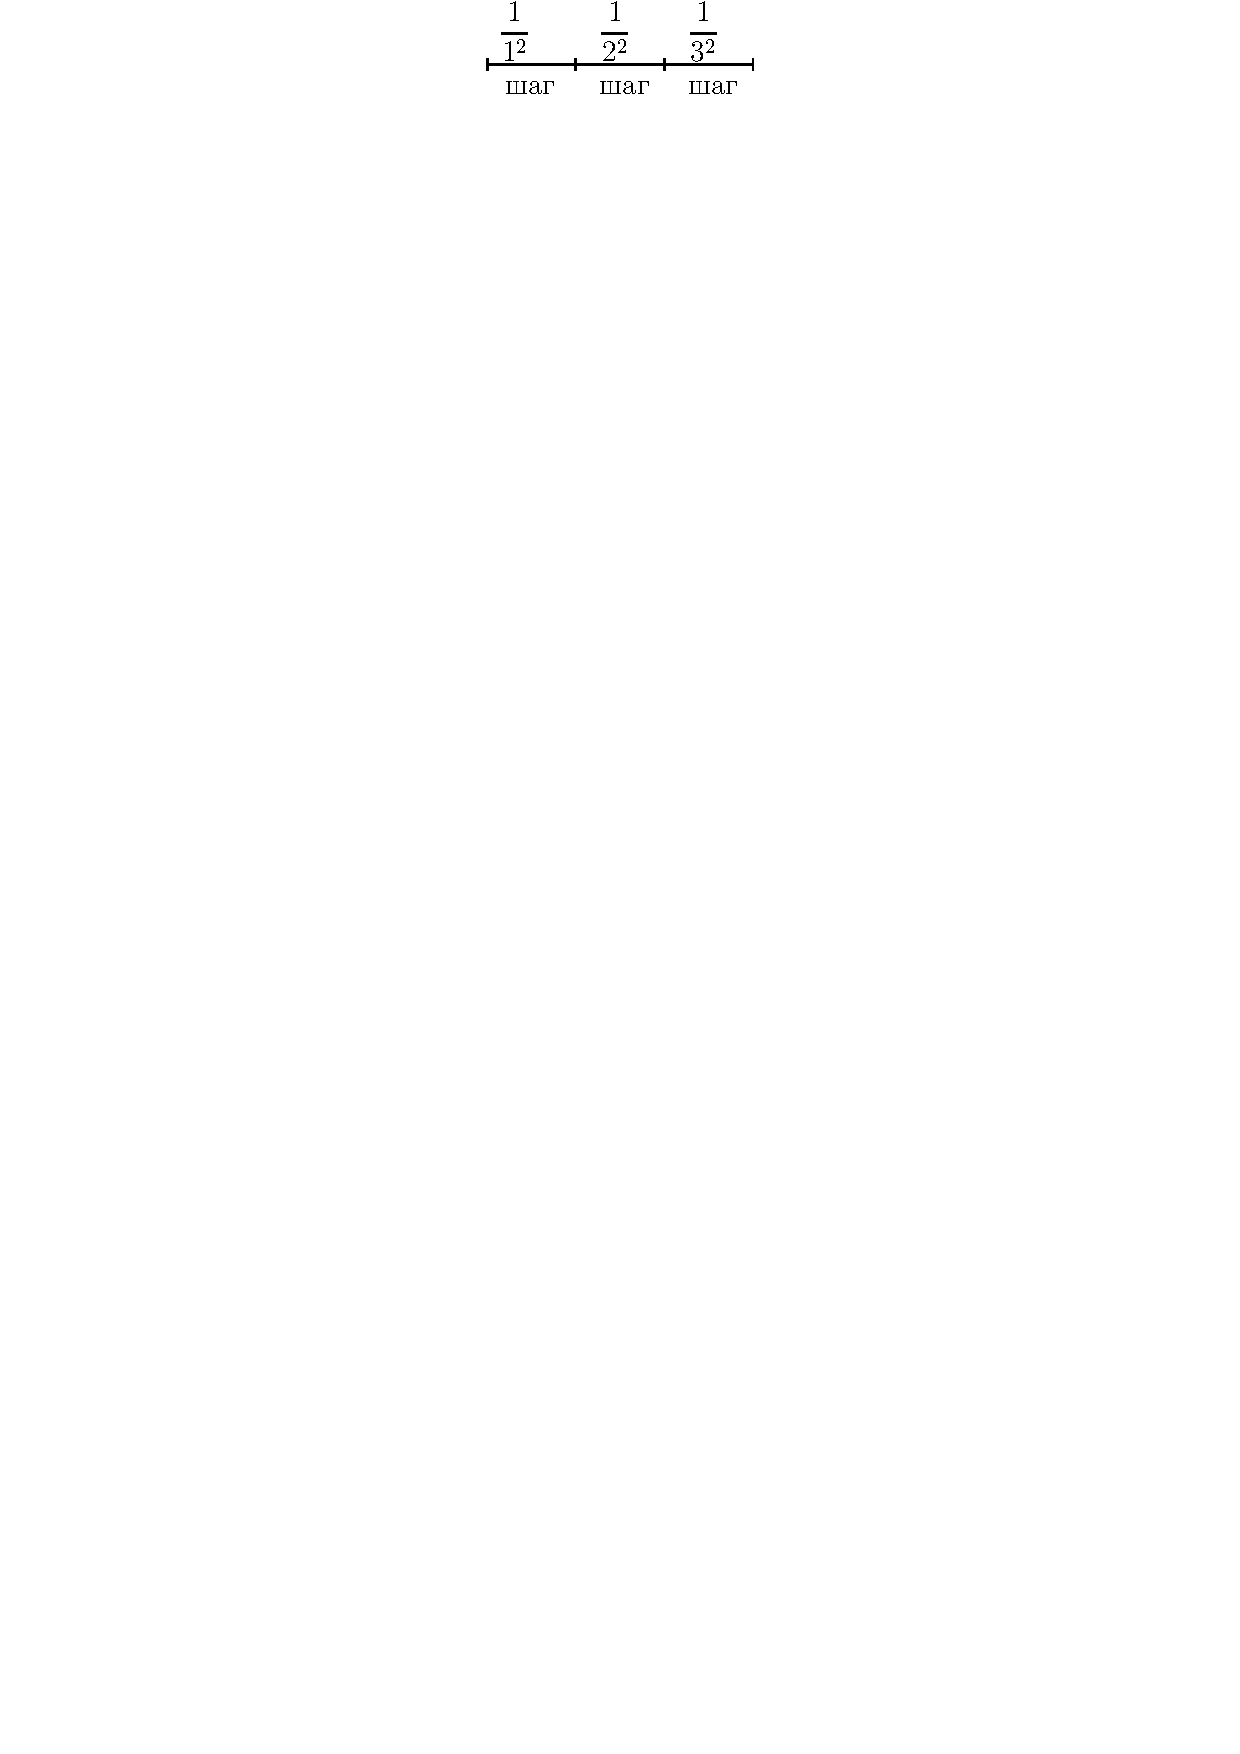
\includegraphics[width=3cm]{img/final/galat/shag.pdf} "--- до бесконечности не дойдём.

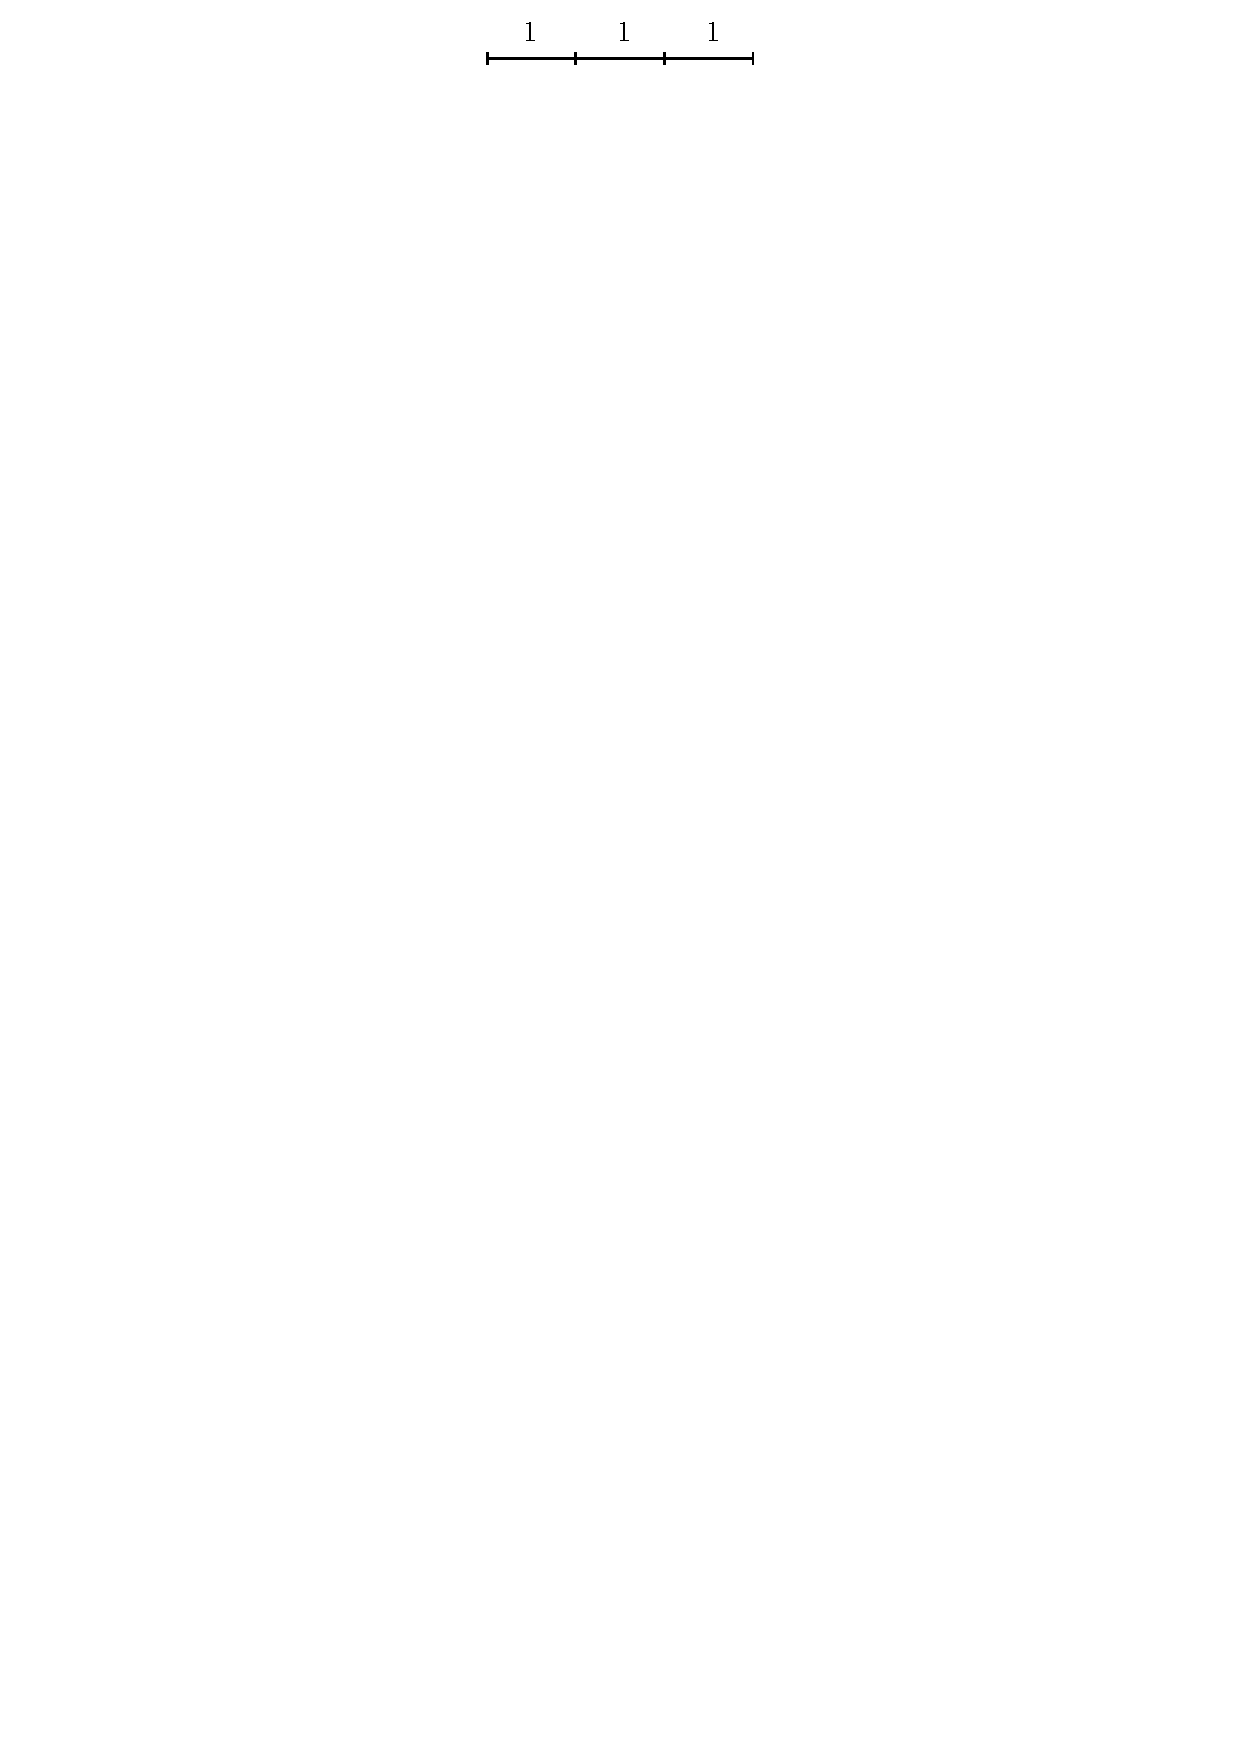
\includegraphics[width=3cm]{img/final/galat/1.pdf} разве можем не дойти до бесконечности? Почему нет? Мало ли бреда в~математике.

$\forall\  \e\hm>0\ \forall\  c\hm>0\ \exists\  m\colon \e m\hm>c$. В~средние века сказали бы «клянусь честью дворянина».
 Также можем сказать: под~$\begin{sideways}
\Big[
\end{sideways}$ контролем, мамой клянусь, гадом буду.

\begin{Proof}
Пусть $\N\hm=\{1,1+1,1+1+1,\ldots\}$ ограниченно сверху, тогда у этого множества существует точная верхняя грань ($\sup$).

$\sup \N\hm=c(\in \R)$.

\begin{enumerate}
    \item Предположим, что в~отрезке $[c-0{,}723,c]$ нет натуральных чисел $\hm{\imp}$ все натуральные числа меньше, чем $c-0{,}723 \hm{\imp} c-0{,}723$ "--- верхняя грань для $\N$. Противоречие с~тем, что $c$ "--- точная верхняя грань;
    \item Если же $\exists\  n\in [c-0{,}723,c]$, то $n+1\hm>c$, противоречие с~тем, что $c$ "--- верхняя грань.
\end{enumerate}
\end{Proof}

\section{Сравнение мощностей}

\begin{Def}
Множества $A$ и $B$ эквивалентны, если существует взаимнооднозначное отображение $A$ на~$B$.

\[A\sim B\]

Вспомним свойства отношения эквивалентности:

\begin{enumerate}
    \item $A\sim A$ "--- рефлексивность;

    \item $A\sim B \hm{\imp} B\sim A$ "--- симметричность;

    \item $A\sim B, B\sim C\hm{\imp} A\sim C$ "--- транзитивность.
\end{enumerate}
\end{Def}

\begin{Def}
Если множество $A$ эквивалентно некоторому подмножеству множества $B$, то говорят, что мощность $A$ не превосходит мощности $B$.
 То есть $A$ эквивалентно подмножеству $B \hm{\iff} \exists$ инъективное отображение $A$ в~$B$.

\end{Def}
$\card A\leq \card B$\pau $|A|\leq|B|$\pau $\#A\leq\#B$.

\begin{Ut}
\begin{enumerate}
    \item $\forall\  A,B\pau \card A\leq \card B$ или $\card B\leq \card A$ "--- доказываем целый семестр на~спецкурсе;

    \item Если $\card A\leq \card B$ и $\card B\leq \card A \hm{\imp} A\sim B$ "--- теорема Кантора-Бернштейна;

    \item Если $\card A\leq \card B$ и $\card B\leq \card C\hm{\imp}
    \card A\leq \card C$.
\end{enumerate}
\end{Ut}

\begin{Proof}(3)
    $\exists\ \phi\colon A\xrightarrow{\text{инъекция}}B,\
    \psi\colon B\xrightarrow{\text{инъекция}} C\hm{\imp} \psi\circ\phi\colon A\to C$ "--- тоже инъекция.
\end{Proof}

Кажется, началось. Мы честно признаёмся, что свойства 1 и 2 идут без доказательства.

\begin{Def}
Множество $A$ состоит из~$n$ элементов, если $A\sim\{1,2,3,\ldots,n\}$, то есть можем элементы пересчитать. Всего $n!$ способов пересчитать.
\end{Def}

\begin{Ut}
Если множество $A$ состоит из~$n$  элементов, $a\nin A$, то $A\cup \{a\}$ состоит из~$n+1$ элемента.
\end{Ut}

\begin{Proof} Рисунок \ref{dobvyk}
\begin{figure}[htbp]\centering
    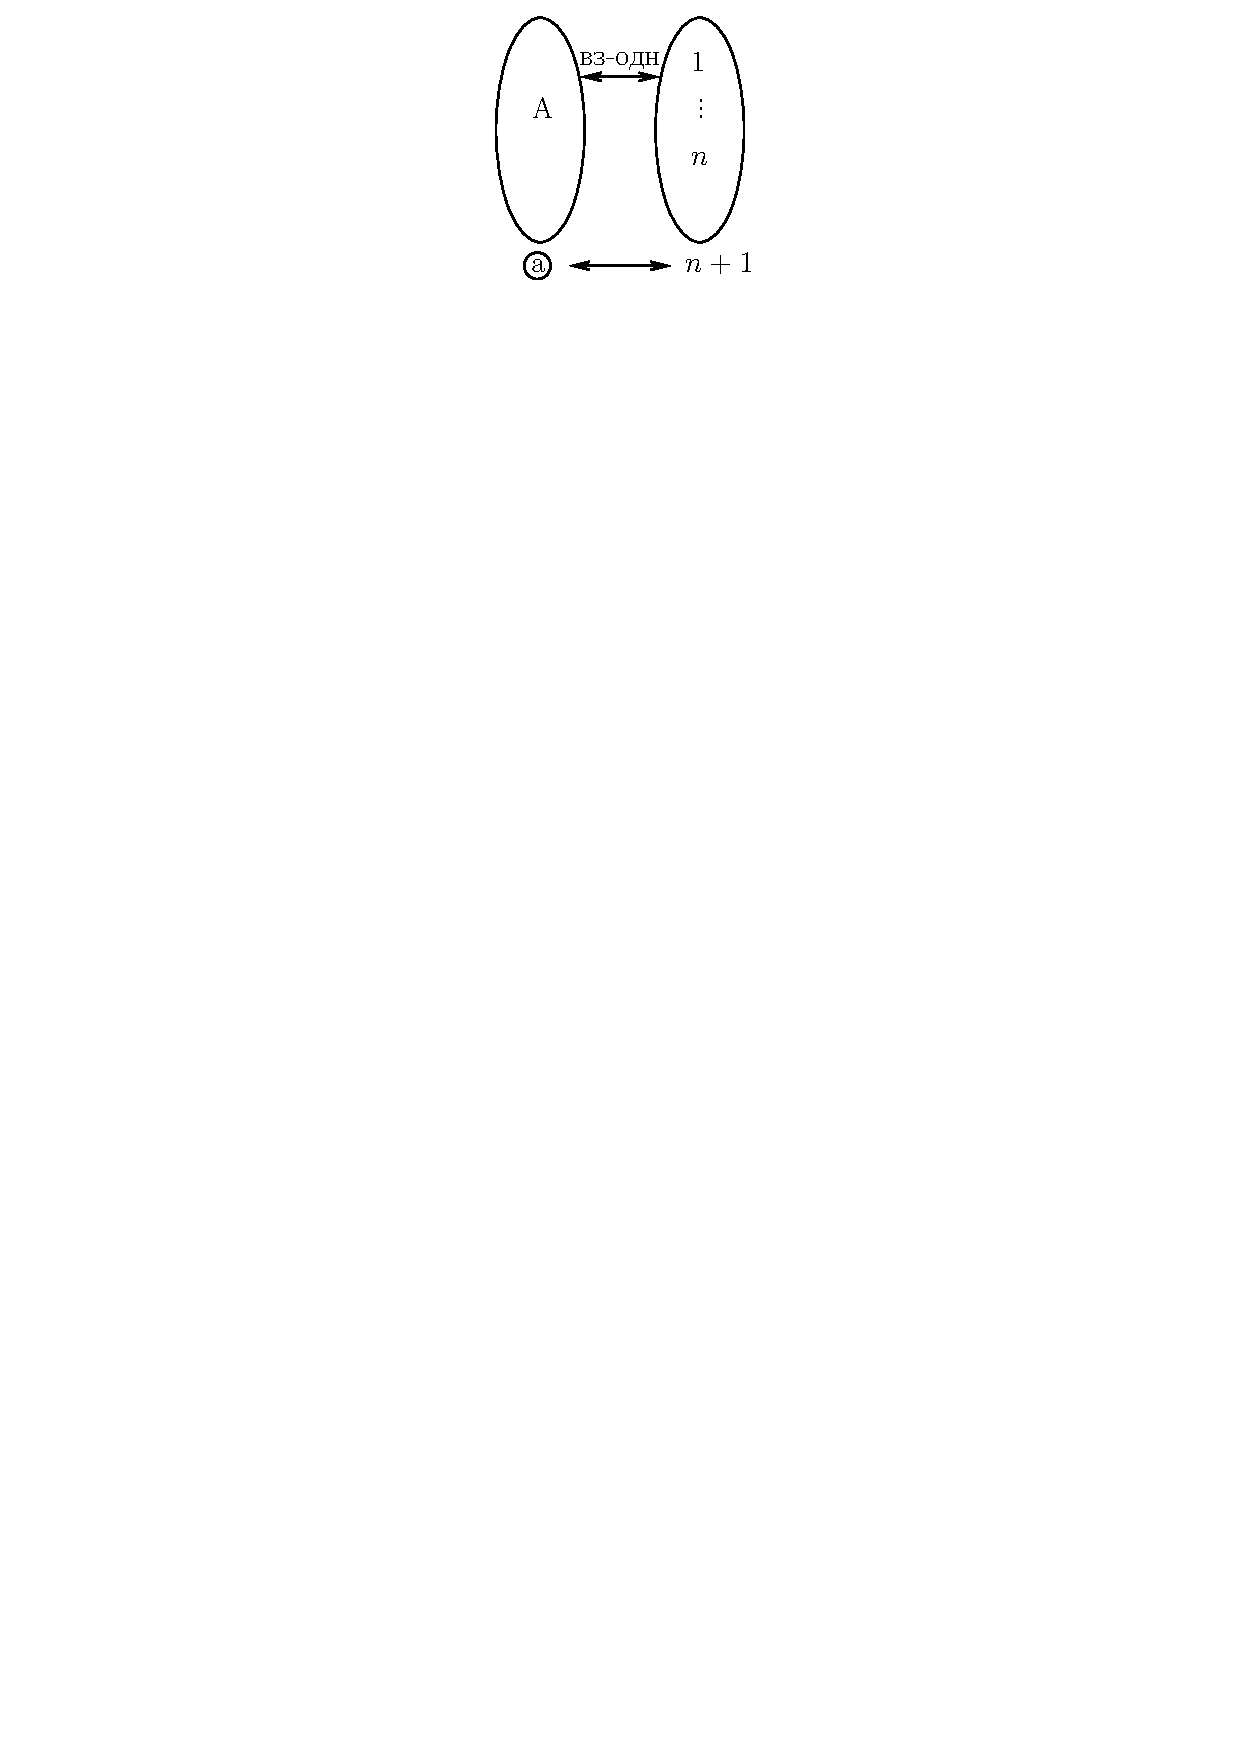
\includegraphics[width=3cm]{img/final/galat/7/mnpo.pdf}
    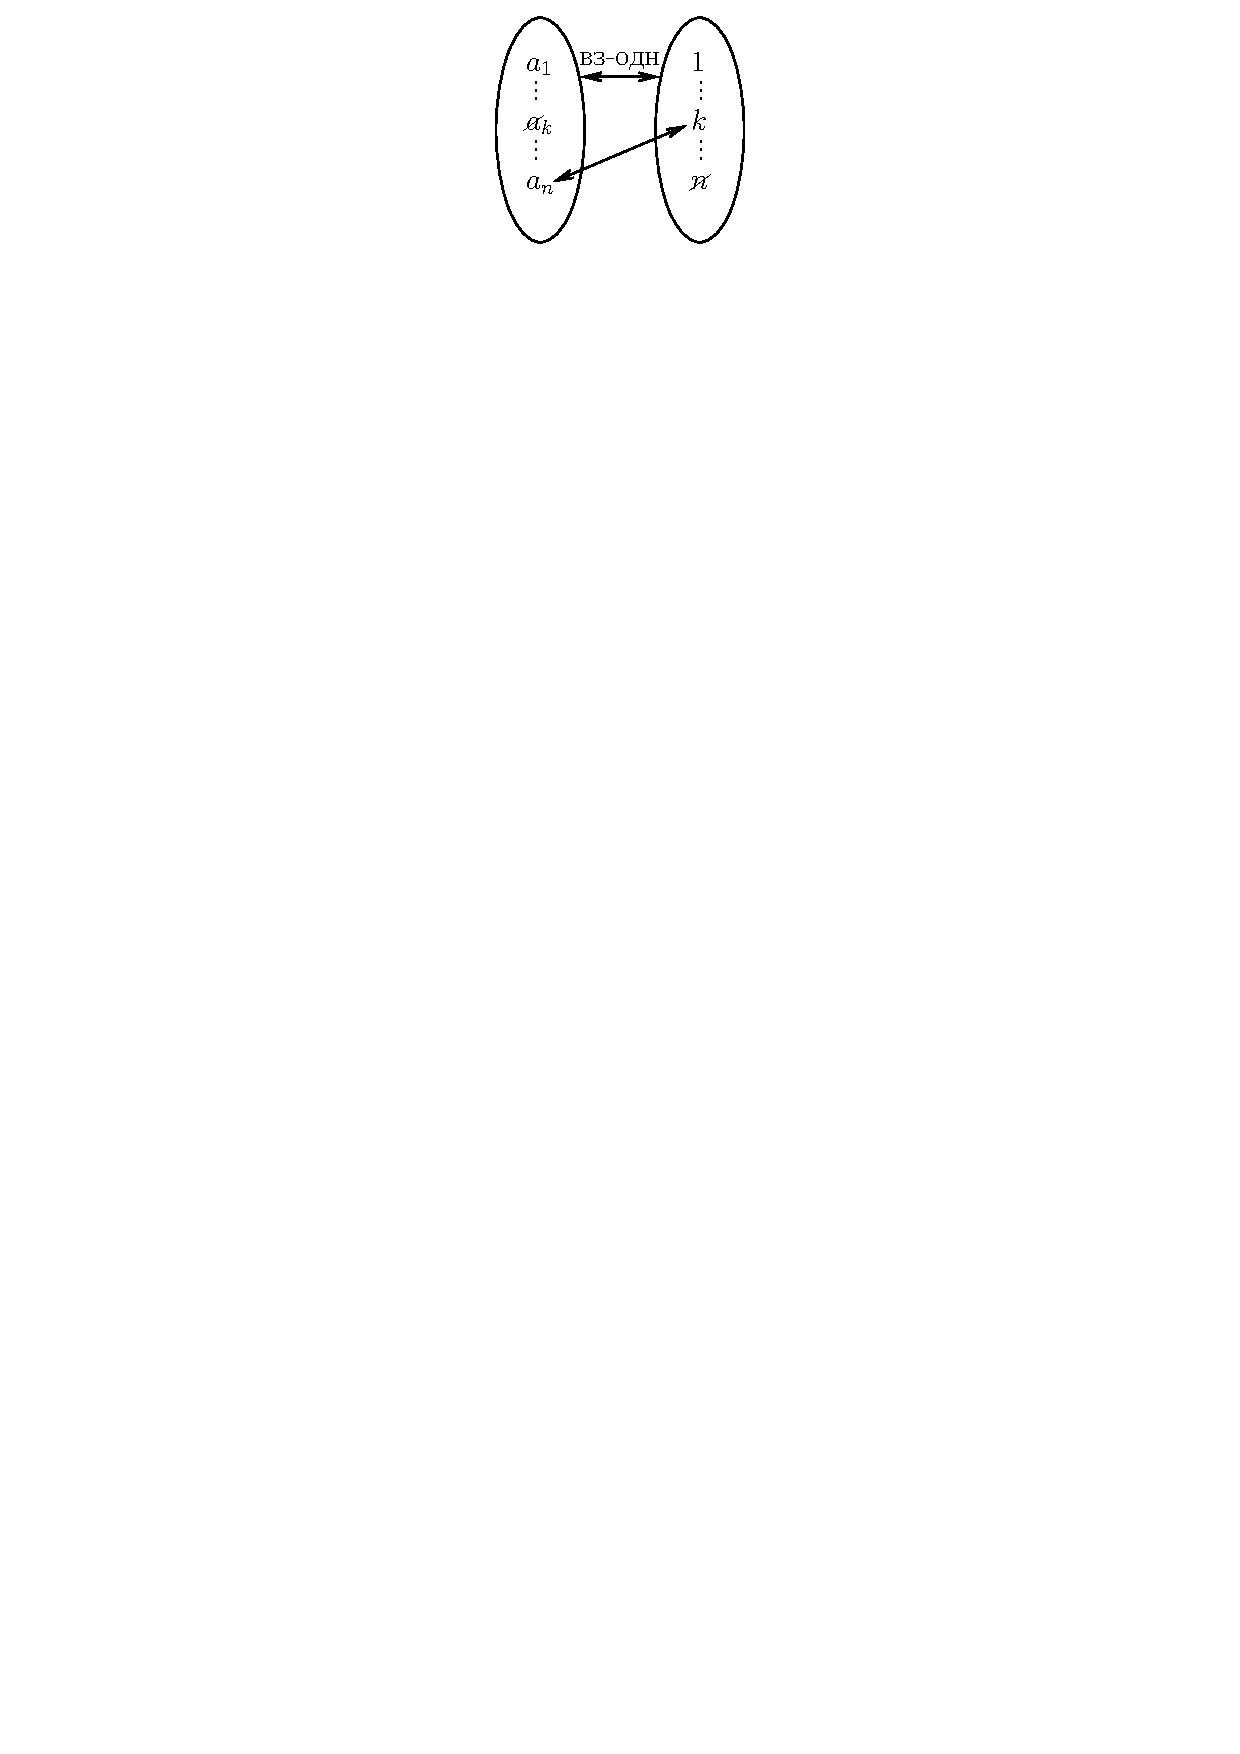
\includegraphics[width=3cm]{img/final/galat/7/mnm1.pdf}
    \caption{Добавление и выкидывание элементов}\label{dobvyk}
\end{figure}
\end{Proof}

\begin{Ut}
Если множество $A$ состоит из~$n$ элементов и $a\in A$ то $A\dd\{a\}$ состоит из~$n-1$ элемента.
\end{Ut}

\begin{Proof}

Пусть $a_n$ теперь соответствует $k$. а~можно и иначе: подвинуть $a_{k+1},\ldots,a_n$ на~одну позицию вверх.

Было: $\phi\colon A\Tot{вз-одн}\{1,\ldots,n\}$, $\phi(a)\hm=k$.

$\psi(b)\hm=\begin{cases}
    \phi(b),&\text{если } \phi(b)\hm<k;\\
    \phi(b)-1,&\text{если }\phi(b)\hm>k.
\end{cases}$

$\psi\colon A\lra\{1,\ldots,n\}$.
\end{Proof}

Ещё парочка определений:

\begin{Def}
Будем говорить, что пустое множество состоит из~нуля элементов.
\end{Def}

\begin{Def}
Множество называется конечным, если оно состоит из~$n$ элементов для некоторого $n\in \N\cup\{0\}\hm=\Z_+$.
\end{Def}

\begin{Def}
Множество называется бесконечным, если оно не является конечным.
\end{Def}

\begin{Def}
Множество называется счётным, если оно эквивалентно множеству $\N$.
\end{Def}

\begin{Def}
Множество называется \textbf{не более чем счётным}, если оно конечно или счётно.
\end{Def}

\begin{Ut}
Любое бесконечное множество имеет счётное подмножество.
\end{Ut}

\begin{Proof}
Пусть $A$ "--- бесконечное множество. Возьмём в~качестве $a_1$ произвольный элемент множества $A$. Положим $A_1\hm=A\dd\{a_1\}$.

$A_1\neq\q$, иначе $A$ конечно.

Возьмём в~качестве $a_2$ произвольный элемент $A_1$, положим $A_2\hm=A_1\dd\{a_2\}\hm=A\dd\{a_1,a_2\},\ A_2\neq\q$.

Предположим, что уже выбраны элементы $a_1,\ldots,a_n$, при этом
$A_n\hm=A\dd\{a_1,\ldots,a_n\}\pau A_n\neq\q$.
В качестве $a_{n+1}$ выберем произвольный элемент $A_n$
$\big(a_{n+1}\nin\{a_1,\ldots,a_n\}\big)$, положим $A_{n+1}\hm=
A_n\dd\{a_{n+1}\}\hm=A\dd\{a_1,\ldots,a_{n+1}\}$. Индуктивно продолжим процесс, выбрав для каждого $n$ по~элементу.
 Получим подмножество $\{a_1,\ldots,a_k,\ldots\}$ "--- подмножество, эквивалентное $\N$.

Чтобы определение было корректно: раз у нас $a_1,\ldots$ все попарно различны, значит биективность с~$\N$ есть.
\end{Proof}

\textit{Скорость чтения лекции может резко возрасти. Я~вообще пишу на~доске, чтобы как-то себя затормозить.
 И когда лектор хорошо знает, что он сейчас будет рассказывать, он пишет быстро.
  Я~"--- хороший лектор, я~не сразу понимаю, что рассказываю.}

Почти все теоремы сегодня Кантора.

\begin{The}\label{Kantor}
Объединение не более чем счётной совокупности не более чем счётных множеств не более чем счётно.
\end{The}

\textit{Ещё интереснее звучит такое, кстати очень серьёзное утверждение: «тощее множество не может быть полным».}

\textit{Давайте я, наконец, пожелаю всем собравшимся приятного аппетита и мы продолжим.}

\begin{Proof}
Пусть $\Big\{A_k\Big\}_{k\hm=1}^{\mathcal{K}} \mathcal K\in\N\cup\{+\infty\}$ "--- не более
 чем счётная совокупность не более чем счётных множеств $A_k\hm=\{a_1^k,a_2^k,\ldots\}$.

Нужно их все прообъединять.

\pic{galat/7/usmn}{2}{trec}{Траектория}

 Табличка может быть бесконечной вправо, может быть бесконечной вниз.

 Не нравится ходить по~диагонали? Военные, например, любят, когда всё прямо и перпендикулярно.
 \pic{galat/7/usmnpr}{3}{ptrec}{Прямая траектория}


Будем нумеровать элементы $\bigcup\limits_k A_k$. Начинаем с~элемента $a_1^1$. Он будет первый,
 следующим будет номер два. Делаем шаги в~соответствии с~нарисованной траекторией.
  Если клетка пустая или содержит элемент, который уже встречался, то (ничего не делаем) и переходим на~следующую клетку, в~противном случае приписываем элементу
следующий номер и увеличиваем следующий номер на~единицу и переходим в~следующую клетку.

\pic{galat/7/mni}{2.2}{mni}{Шаги по~траектории}


Пройдём всё, потому что на~$a^j_i$ наступим за число шагов, которое можно найти.
\end{Proof}

\begin{Sl}
\begin{tabular}{llll}
$\Z$&счётно& &$\Z\hm=\N\cup(-\N)\cup\{0\}$ по~теореме \ref{Kantor} Кантора счётно;\\
$\Q$&счётно& &$\Q\hm=\bigcup\limits_{m\in\Z}\left(\bigcup\limits_{n\in \N}\left\{\dfrac mn\right\}\right)$;\\ $\mathbb{A}$&счётно& &
\end{tabular}
\end{Sl}

\begin{Proof} Действительно: $\left\{\dfrac mn\right\}$ "--- конечное множество из~одного элемента. $\bigcup\limits_{n\in\N}$ "--- счётное объединение. $\bigcup\limits_{m\in\Z}$ "--- счётное объединение. В~итоге после всех объединений множество не более чем счётно.

$\mathbb{A}\hm=\{x\in\R\colon x$ являются корнем хоть одного многочлена с~рациональными коэффициентами (всё равно, что с~целыми)$\}$.

\begin{enumerate}
    \item Многочленов степени $n\in\N$ с~фиксированными коэффициентами не более чем счётное множество:
        $\bigcup\limits_{a_n\in\Z}\left(\dots\bigcup\limits_{a_1\in\Z}\bigcup\limits_{a_0\in\Z}\right)\{a_nx^n+a_{n-1}x^{n-1}+\ldots+a_1x+a_0\}$;

    \item Множество чисел являющихся корнями многочлена степени $n\in \N$ конечно, то есть не более чем счётно;

    \item Теперь, объединяя по~$n$ такие множества, получим множество $\mathbb{A}$. Такое гигантское множество, оказывается, тоже счётно.
\end{enumerate}
\end{Proof}

Давайте я~ещё какие-нибудь теоремы напишу.

\begin{Ut}
Подмножество не более чем счётного множества не более чем счётно.
\end{Ut}

\begin{Proof}
$a_1,a_2,\underbrace{a_3}_{b_1},a_4,\ldots\underbrace{\ldots}_{b_2}\ldots$

Идём слева направо и нумеруем.
\end{Proof}

\begin{Ut}
Если $A$ бесконечно, а~$B$ не более чем счётно, то $A\cup B\sim A$.
\end{Ut}

\begin{Proof}
Пусть $A_1$ "--- счётное подмножество $A$, а~$B_1\hm=B\dd A$ "--- не более чем счётно.

$A\cup B\hm=(A\dd A_1)\cup(A_1\cup B_1)$.

Если $A_1\sim B_1,\ A_2\sim B_2, A_1\cap A_2\hm=\q, B_1\cap B_2\hm=\q$, то $(A_1\cup A_2)\sim (B_1\cup B_2)$ "--- это лирика.

\pic{galat/7/er}{1.5}{er}{Эквивалентность объединения непересекаемых}

Итак: $A\cup B\hm=\underset{\sim A\dd A_1}{(A\dd A_1)}\cup
\underset{\sim A_1}{(A_1\cup B_1)}\sim (A\dd A_1)\cup A_1\hm=A$.
\end{Proof}

Оказывается, добавлять "--- глупый процесс. Выкидывать гораздо интереснее.
\section{Бесконечные множества}

Вспомним важное:

\begin{enumerate}
\item $A\sim B\hm{\iff}\exists\  \phi\colon A\Tot{вз-одн}B$.

\item Если $A\sim B_0\subset B, B\sim A_0\subset A$, то $A\sim B$.

\item Любое бесконечное множество имеет счётное подмножество.

\item Объединение не более чем счётной совокупности не более чем счётных множеств не более чем счётно.

\item Если $A_1\sim B_1,A_2\sim B_2,A_1\cap A_2\hm=\q,B_1\cap B_2\hm=\q$,
то $(A_1\cup A_2)\sim (B_1\cup B_2)$.

\item Если $A$ бесконечно, $B$ не более чем счётно, то $(A\cup B)\sim A$.
\end{enumerate}
\begin{Proof}
    $A\cup B\hm=A\cup(B\dd A)$, где $(B\dd A)$ "--- не более чем счётно. 
    $\underset{\sim A\dd A_1}{(A\dd A_1)}\cup\underset{\sim A_1}{\big(A_1\cup( B\dd A)\big)}$.
\end{Proof}

Что можно выкидывать безболезненно?

\begin{Ut}
Если $A$ "--- бесконечно множество, $B$ "--- конечное подмножество $A$, то $A\dd B\sim A$.
\end{Ut}

\begin{Proof}
С учётом индукции достаточно доказать, что $\forall\  a\in A\pau A\dd\{a\}\sim A$ (индукция применяется только для конечного числа выкидываний).

$A\dd \{a\}$ бесконечно (если оно конечно из~$n$ элементов, то $A$ из~$n+1$ "--- тоже конечное, противоречие).

Пусть $A_1$ "--- бесконечное счётное подмножество $A\dd \{a\}$ (которое бесконечно, поэтому и имеет счётное подмножество).

Что такое вообще множество $A$? $A\hm=\Big(A\dd\big(A_1\cup\{a\}\big)\Big)\cup\Big(A_1\cup\{a\}\Big)$.

Глубокий факт: $\Big(A\dd \big(A_1\cup\{a\}\big)\Big)$ эквивалентно себе, а~$\big(A_1\cup\{a\}\big)\sim A_1$.

$A\dd\big(A_1\cup\{a\}\big)\cup\big(A_1\cup\{a\}\big)\sim
\Big(A\dd\big(A_1\cup\{a\}\big)\Big)\cup A_1\hm=
A\dd\{a\}$.
\end{Proof}

\textit{Бесконечная государственная казна, из~которой чиновники берут конечные суммы и знают, что бесконечность остаётся такой же.}


\[(a,b)\sim[a,b]\sim[a,b)\sim(a,b]\sim\left[0;\textstyle\frac{\pi}2\right)\sim\R^+\]

$(0,1)\overset{\underset{/}{\text{ну}}\text{ лин от-ние}}
{\sim\left(-\frac{\pi}2,\frac{\pi}2\right)}\overset{\tg}{\sim}\R
\mspace{72mu}
\phi(x)\colon (0,1)\to(a,b)\mspace{72mu}\phi(x)\hm=x(b-a)$.

\pic{galat/8/sim}{1}{simr}{Гомотетия}



\pic{galat/8/trkv}{3.6}{trkv}{Фигуры на~плоскости эквивалентны}


\begin{Ut}Точек квадрата ровно столько же, сколько в~отрезке.

\[
[0,1]\sim[0,1]^2
\]\end{Ut}

\begin{Proof}
    $\card[0,1]\leq\card[0,1]^2$, задать биективное отображение с~подмножеством квадрата, тривиально.

    Покажем, что $\card[0,1]^2\leq\card[0,1]$.

    Возьмём точку квадрата $(x,y)\hm=(0{,}n_1^xn_2^x\ldots,0{,}n_1^yn_2^y\ldots)$ "--- координаты в~десятичной записи.
     Зададим инъективное отображение, при котором точка $(x,y)$ перейдёт в~$(0{,}n_1^xn_1^y2n_2^xn_2^y2n_3^xn_3^y\ldots)$.

    Проблема: $0{,}111111\ldots,0{,}1\underset{\text
    {запрещённые девятки}}{9999999999999999999}\ldots\to0{,}112192192192\ldots$ "--- ни один
     образ не будет содержать периодическую девятку с~таким порядком записи. Итак, мы установили взаимнооднозначное
      отображение множества точек квадрата на~подмножество (ведь есть точки ещё и без двоек через каждые три цифры, например) отрезка.

    Применяем теорему Кантора"--~Бернштейна и всё собственно.
\end{Proof}

Фундаментальная теорема математики была бы о том, что бесконечность везде одинакова. Но это не так.

\begin{The}
    $[0,1]$ "--- не счётное множество.
\end{The}

\begin{Proof}\textbf{1.}

    Пусть $\phi$ "--- инъективное отображение $\N\to[0,1)$. Достаточно показать, что оно не сюръективное.
    Введём следующие обозначения: пусть $\phi(n)\hm=0{,}k_1^nk_2^nk_3^n\ldots$ (запись без периодических девяток).

    Пусть $x\hm=0{,}a_1a_2a_3a_4\ldots$, где $a_j\hm=
    \begin{cases}
        3,&\text{если } k_j^j\neq3\\
        7,&\text{если } k_j^j\hm=3
    \end{cases}$ (периодическая девятка невозможна).

    $\forall\  j\in\N\pau x\neq\phi(j)$ "--- отличие по~крайней мере в~$j$-ом разряде, а~периодическая девятка запрещена.
    Значит, $\phi$ не сюръективно (ну и не биективно). Чуть подробнее: у нас есть образ $\phi(\N)$, он состоит из~кучи действительных чисел
    $\phi(1),\phi(2),\ldots$. Глядя на~эти $\phi(j)$ строим плохое число: ноль целых и что-то после запятой. 
    Первую цифру после запятой ставим не такую, как в~$\phi(1)$, вторую "--- не такую, как в~$\phi(2)$ и так далее.
     Это число не будет равняться никакому $\phi(j)$, но оно точно есть в~$[0,1]$ и без периодических девяток, 
     потому что там исключительно $3$ или $7$. Вот и развалилась сюръективность.

\end{Proof}

$\begin{matrix}
    \phi(1)\hm=&0{,}\boxed{k_1^1}k_2^1k_3^1\ldots\\
    \phi(2)\hm=&0{,}k_1^2\boxed{k_2^2}k_3^2\ldots\\
    \phi(3)\hm=&0{,}k_1^3k_2^3\boxed{k_3^3}\ldots\\
    \ldots&\ldots\ldots
\end{matrix}$ "--- в~рамках цифры, которые не дают совпасть $\phi(j)$ с~заданным иксом.

\begin{Proof}\textbf{2}

    Пусть $\phi(n)$ "--- произвольное инъективное отображение $\N\to [0,1]$. Достаточно доказать, что $\phi$ не сюръективно.


    \pic{galat/8/otr}{1.35}{otr}{Отрезок}



    Обозначим $\phi(n)$ через $x_n$. Положим $\Delta_0\hm=[0,1]$. В~качестве $\Delta_1$
     выберем произвольную треть (являющуюся именно отрезком) отрезка $\Delta_0$, не содержащую $x_1$.
\pic{galat/8/delta1}{1.35}{delta1}{Выбор вложенного отрезка}


Если уже построен отрезок $\Delta_n$, то в~качестве отрезка $\Delta_{n+1}$ берём произвольную треть
 отрезка $\Delta_n$, не содержащую $x_{n+1}$. Построена последовательность вложенных отрезков $\Big\{\Delta_n\Big\}_{n\hm=0}^{\infty}$.

В соответствии с~принципом Кантора \ref{ppk} о вложенных отрезках существует общая точка этих отрезков,
 обозначим её за $x$. Ни для одного $n\in\N\pau x\neq x_n\hm=\phi(n)\pau x\in\Delta_n\nni x_n$.


\end{Proof}

\textit{Отношение к~хлебу определяет моральный облик общества.}

\begin{Def}
    Множества, эквивалентные $[0,1]$ называются \textbf{континуальными}.
\end{Def}

\begin{Sl}
    Множества иррациональных чисел континуально. Множество трансцендентных (то есть не алгебраических) чисел тоже континуально.
\end{Sl}

\begin{Proof}
    В~любом отрезке существует хоть одно иррациональное число, кроме того их бесконечное множество.
     Факт не тривиальный. Давайте смотреть: если это множество не более, чем счётно, то


    Отрезок$\hm=\underset{\text{счётно}}{\{\text{множеству рациональных чисел отрезка}\}}\cup\{$множество иррациональных чисел отрезка$\}\hm{\imp}$ Отрезок "---счётное множество.

    Или ещё так: $\underset{\text{беск}}{\Big([0,1]\dd \Q\Big)}\cup\underset{\text{сч.}}{\Q}\sim[0.1]\dd \Q$.
\end{Proof}


Пусть $A$ "--- счётное множество. $\mathscr A$ "--- совокупность всех его подмножеств.

\begin{The}[Кантора]
$\card A\hm<\card\mathscr A$.
\end{The}

\begin{Proof}
    \begin{enumerate}
        \item Инъективное отображение $A\to \mathscr A$\pau $a\to\{a\}\hm{\imp}\card A\leq\card \mathscr A$ "--- тривиальная часть;

        \item Покажем, что $\card A\hm<\card\mathscr A$. Пусть $\phi$ "--- произвольное инъективное отображение $A\to \mathscr A$. Достаточно показать, что оно не сюръективно.
            Обозначим образ $\phi(a)$ через $A_a$;

            Положим, что множество $B\hm=\Big\{a\in A\colon a\nin A_a\Big\}$. Ни для одного элемента $a\in A$ множество $B$ не совпадает с~$A_a$. Почему? а~вот, почему:
    \end{enumerate}

            Пусть $a$ "--- произвольный элемент $A$. Покажем, что $B\neq A_a$. Действительно, пусть $B\hm=A_a$ для некоторого $a_0\in A$, тогда

            \begin{enumerate}
                \item $a_0\in A_{a_0}(\hm=B)\hm{\imp} a_0\nin B$ (принадлежит $A_{a_0}$, значит \textbf{не должен} принадлежать $B$). Одновременно входит и не входит;

                \item $a_0 \nin A_{a_0}(\hm=B) \hm{\imp} a_0$ должен $\in B$.
            \end{enumerate}

            Мораль: противоречие.

\end{Proof}

\section{О точках}
\begin{Def}
    Двузначная последовательность "--- последовательность двух элементов множества.
\end{Def}

$\ro$ "--- множество всех последовательностей из~$0$ и $1$.

\begin{Ut}
    $\ro$ континуально. (то есть $\ro\sim[0,1]$).
\end{Ut}

\begin{Proof}
    \begin{enumerate}
        \item Пусть $x$ "--- произвольное число отрезка $[0,1]$.

            Запишем $x$ в~двузначной записи $x\hm=0{,}n_1n_2n_3n_4\ldots\pau \Big(n_i\in\{0,1\}\Big)$. Для тех, кому не нравятся $0,1$ пишем «лево», «право».


\pic{galat/9/levo}{1.2}{levo}{Альтернатива нулям и единицам в~отрезке}

Соответственно $[0,1]\ni x\to \underset{\in\ro}{n_1n_2n_3}\ldots$ инъективно. Значит, $\card [0,1]\leq\card\ro$.

Для $\frac 12\to\begin{cases}
    0{,}10000\\
    0{,}01111\ldots
\end{cases}$ "--- но мы выберем одно, задавая отображение $\hm{\imp}$ не биективно.

\item Пусть $n_1n_2n_3\ldots\in\ro$. Сопоставим ей число $x$ отрезка $[0,1]$.

    $x\hm=0{,}n_1n_2n_3\ldots$ "--- десятичная запись (я же не хочу получить все числа, $n$ здесь только $1$ или $0$).

    Это инъективное отображение $\ro$ в~$[0,1]$. Мощность $\card\ro\leq\card[0,1]$. По~теореме Кантора-Бернштейна вывод: $\card\ro\hm=\card[0,1]$.
    \end{enumerate}
\end{Proof}

\subsection{А теперь рассмотрим подмножества расширенной прямой}

Пусть $x$ "---точка действительной прямой, а~$\e\hm>0$.

\begin{Def}
    $\e$-окрестностью точки $x$ называется интервальчик $(x-\e,x+\e)$. Обозначается $B_\e(x)$.

    Проколотая $\e$-окрестность точки $x\colon(x-\e,x+\e)\dd\{x\}$. Обозначается $B'_\e(x)$.

    На~$\R\colon B_\e(+\infty)\hm=B'_\e(+\infty)\hm=(\frac{1}{\e},+\infty)$ "---
    ($\frac 1\e$ чтобы при увеличении $\e$ окрестность сужалась). $B_\e(-\infty)\hm=(-\infty,-\frac 1\e)$.

    На~$\ol\R\colon B_\e(+\infty)\hm=(\frac{1}{\e},+\infty],B'_\e(+\infty)\hm=(\frac{1}{\e},+\infty)$. Для $-\infty$ аналогично.
\end{Def}

Окрестность "--- субъективно маленький интервал.

Пусть $A\subset\R(\ol\R)$

\begin{Def}
    Точка $x$ называется внутренней точкой множества $A$, если $x$ входит в~$A$  с~некоторой своей окрестностью, то есть:

    \[
        \exists\ \e\hm>0\colon B_\e(x)\subset A
    \]
\end{Def}

\begin{Def}
    Точка $x$ называется внешней точкой множества $A$, если $x$ входит в~дополнение $A$ с~некоторой своей окрестностью, то есть:

    \[
        \exists\  \e\hm>0\colon B_\e(x)\cap A\hm=\q
    \]
\end{Def}

\begin{Def}
    Точка $x$ называется \textbf{граничной} точкой множества $A$, если она не является ни внутренней, ни внешней, то есть:

    \[
        \forall\  \e\hm>0\pau B_\e(x)\cap A\neq\q, B_\e(x)\cap\ol A\neq\q
    \]

    $\ol A\hm=\R\dd A$ или $\ol\R\dd A$.
\end{Def}

\begin{Def}
    Точка $x$ называется изолированной точкой множества $A$, если $\exists\ \e\hm>0\colon B_\e(x)\cap A\hm=\{x\}$.
\end{Def}

\begin{Def}
    Множество $A$ называется открытым, если все его точки внутренние. То есть:

    \[
        \forall\  x\in A\pau\exists\  \e\hm>0\colon B_\e(x)\subset A
    \]

\end{Def}

\begin{Def}
    Множество $A$ называется замкнутым, если его дополнение открыто.
\end{Def}

Интервал "--- открытое множество, отрезок "--- замкнутое, полуотрезок, рациональные числа "--- никакие множества. Подмножеств отрезка "--- гиперконтинуум,
 замкнутых множеств континуум.

$\q,\R$ "--- и открыты и замкнуты.

\subsubsection*{Почему других открытых и замкнутых нет?} Можно делить отрезки пополам, если обе половины открыты, то одна точка окажется между.

\subsubsection{Свойства}

\begin{Ut}
    Множество открыто $\hm{\iff}$ оно не содержит ни одной граничной точки.
\end{Ut}

\begin{Ut}
    Множество замкнуто $\hm{\iff}$ оно содержит все свои граничные точки.
\end{Ut}

\begin{Pre}
    Точка $x$ является граничной точкой $A \hm{\iff}$ является граничной точкой $\ol A$.
\end{Pre}

Вариант-исключение, когда граничных точек нет.

$\ol{\ol A}\hm=\ol{(\ol A)}\hm=A$

\begin{Ut}
    Объединение \textbf{произвольной} совокупности открытых множеств "--- открытое множество. Пересечение \textbf{конечной} совокупности открытых множеств "--- открытое множество.
\end{Ut}

Если издеваться, но не сильно, открытость сохраняется.

\begin{Proof}
    Пусть $\Big\{G_\lambda\Big\}_{\lambda\in\Lambda}$
    "--- совокупность открытых множеств. $x$ "--- произвольная точка из~$\bigcup\limits_{\lambda\in\Lambda}G_\lambda$.
    Тогда $\exists\ \lambda_0\colon x\in G_{\lambda_0}$,
    так как $G_{\lambda_0}$ открытое $\exists\ \e\hm>0\colon B_\e(x)\subset G_{\lambda_0}
    \hm{\imp} B_\e(x)\subset\bigcup\limits_{\lambda\in\Lambda}G_\lambda$. Значит $\bigcup\limits_{\lambda}G_\lambda$ открыто.

    Пусть $C_1\ldots,C_N$ "--- открыты. $x$ "--- произвольная точка
    $\bigcap\limits_{n\hm=1}^{N}C_n\hm{\imp}$

    $\hm{\imp} x\in C_1\hm{\imp}\exists\  \e_1\hm>0\colon B_{\e_1}(x)\subset C_1$

    $x\in C_2\hm{\imp}\exists\ \e_2\hm>0\colon B_{\e_2}(x)\subset C_2$

    $\vdots$

    $x\in C_N\hm{\imp}\exists\ \e_N\hm>0\colon B_{\e_N}(x)\subset C_N$

    Положим $\e\hm=\min\{\e_1,\ldots,\e_N\}$ "--- в~конечном наборе наименьший точно найдётся (именно поэтому верно только для пересечения конечной совокупности).

    Тогда $\forall\  n\in\{1,\ldots,N\}\pau B_\e(x)\subset C_n\hm{\imp} B_\e(x)\subset
    \bigcap\limits_{n\hm=1}^NC_n$. Значит, $\bigcap\limits_{n\hm=1}^NC_n$ открыто.
\end{Proof}

Бесконечное пересечение ведёт себя по-разному: иногда хорошо:
$\bigcap\limits_{n\in \N}\left(-\dfrac1n,1+\dfrac1n\right)\hm=[0,1]$,

Иногда не очень:
 $\bigcap\limits_{n\in \N}\left(-\dfrac1n,1\right)\hm=[0,1)$.

 \begin{Sl}
Пересечение \textbf{произвольной} совокупности замкнутых множеств "--- замкнуто. Объединение \textbf{конечной} совокупности замкнутых множеств "--- замкнутое множество.
 \end{Sl}

 \begin{Proof}
$\Big\{\mathcal{F}_\lambda\Big\}_{\lambda\in\Lambda}$ "--- совокупность замкнутых множеств.
$\bigcap\limits_{\lambda\in\Lambda}\mathcal{F}_\lambda\underset{\ref{Themor}}{\hm=}
\bigcup\limits_{\lambda\in\Lambda}\ol{{\mathcal F}_\lambda}$ "--- объединение открытых множеств открыто.
 \end{Proof}

 \begin{Def}\label{pt}
Точка $x$ называется предельной точкой множества $A$, если в~любой проколотой окрестности $x$ есть хоть одна точка множества $A$, то есть:

\[
    \forall\  \e\hm>0\pau B'_\e(x)\cap A\neq \q
\]
 \end{Def}

 \begin{The}\label{hal}
Следующие утверждения эквивалентны:

\begin{enumerate}
    \item $x$ "--- предельная точка $A$.

    \item $\forall\  \e\hm>0\ B'_\e(x)\cap A$ "--- бесконечное множество.

    \item $\forall\  \e\hm>0\ B_\e(x)\cap A$ "--- бесконечное множество.
\end{enumerate}
 \end{The}

 \begin{Proof}
$2\hm{\iff} 3$ это понятно, они отличаются максимум на~одну точку.

$2\hm{\imp} 1$ халява: по~определению.

Осталось $1\hm{\imp} 2$. От противного для скорости: пусть $\exists\ \e\hm>0\colon B'_\e(x)\cap A$ конечно. Пусть это пересечение состоит из~точек $\big\{a_1,\ldots,a_N\big\}$. Положим $\e_0\hm=\min\big\{|x-a_1|,|x-a_2|,\ldots,|x-a_N|\big\}\hm>0$.

Тогда $B'_{\e_0}(x)\cap A\hm=\q$ "--- противоречие с~тем, что $x$ есть предельная точка.
 \end{Proof}

 \begin{Ut}
Множество замкнуто $\hm{\iff}$ оно содержит все свои предельные точки.
 \end{Ut}

 \begin{Proof}
Пусть $A$ "--- замкнуто, $x\nin A$. Достаточно доказать, что $x$ не предельная точка.

Так как $A$ замкнуто, $x$ "--- внешняя точка $A$, то есть
 $\exists\ \e\hm>0\colon B_\e(x)\cap A\hm=\q$, значит $x$ не предельная точка.

 Пусть $A$ содержит все свои предельные точки. Покажем, что $A$ замкнуто.
 Пусть $x$ "--- произвольная точка из~$\ol A$. Тогда $x$ не предельная точка $A$.

 $\exists\ \e\hm>0\colon B'_\e(x)\cap A\hm=\q$. Так как $x\nin A$, то $B_\e(x)\cap A\hm=\q$, то есть $x$ "--- внешняя точка $A$. Следовательно $\ol A$ "--- открыто, $A$, стало быть, замкнуто.
 \end{Proof}

 \section{Теорема Больцано"--~Вейерштрасса}

 Мы работаем с~множеством $A\subset\R(\ol\R)$

 \begin{Def}
$x$ "--- предельная точка $A$, если $\forall\ \e\hm>0\ B'_\e(x)\cap A\neq \q$ или эквивалентно $\forall\  \e\hm>0\ B'_\e(x)\cap A$ бесконечно.
 \end{Def}

 \begin{The}[Больцано"--~Вейерштрасса о существовании предельной точки]\label{bolc} Любое бесконечное ограниченное подмножество  $\R$ имеет (хоть одну) предельную точку на~$\R$.
\end{The}

\begin{Proof}
    Метод имени Цезаря: Пусть $A$ "--- произвольное бесконечное ограниченное подмножество $\R$. Найдём $c\hm>0\colon A\subset[-c,c]$ (используем ограниченность).
    Положим $\Delta_0\hm=[-c,c]$.

    Метод copy-paste. В~качестве отрезка $\Delta_1$ возьмём произвольную половину $\Delta_0\colon A\cap \Delta_1$ бесконечно. В~качестве $\Delta_2$ возьмём произвольную половину $\Delta_1\colon A\cap\Delta_2$ бесконечно и так далее.

    Если уже построен $\Delta_n\colon A\cap \Delta_n$ бесконечно, то в
    качестве $\Delta_{n+1}$ возьмём произвольную половину $\Delta_n\colon \Delta_{n+1}\cap A$ бесконечно.

    Получили последовательность вложенных отрезков: $\Big\{\Delta_n\Big\}_{n\hm=0}^{\infty}\colon \forall\  n\in \N\pau A\cap\Delta_n$ бесконечно. $|\Delta_n|\hm=\dfrac{2c}{2^n}$.

    Докажем такую лемму:

    \begin{Th}\label{perednosom}
        $\forall\ \e\hm>0\pau \forall\  \tilde c\hm>0\pau \exists\ \ N\in\N\colon \forall\  n\hm>N\pau \dfrac{\tilde c}{2^n}\hm<\e$
    \end{Th}

    \begin{proof}
        Найдём $N\hm>\dfrac{\tilde c}{\e}$ (используем принцип Архимеда \ref{arhy}).
         Тогда $\forall\  n\hm>N\pau 2^n\hm>2^N\hm=(1+1)^N\underset{\ref{Bern}}{\geq} 1+N\cdot1\hm>N\hm>\dfrac{\tilde c}{\e}$
        Отсюда $\dfrac{\tilde c}{2^n}\hm<\e$

    \end{proof}

    по~принципу Кантора \ref{ppk} $\exists\  x_0$ общая точка $\Big\{\Delta_n\Big\}_{n\hm=0}^\infty$. Покажем, что точка $x_0$ предельная точка $A$.

\pic{galat/10/dance}{2.5}{dance}{Танец отрезка в~окрестности}


    по~определению возьмём произвольное $\e\hm>0$. Найдём $n\colon \dfrac{2c}{2^n}\hm<\e$ (по лемме, которая перед носом). Тогда $\Big(B_\e(x_0)\cap A\Big)\supset\Big(\Delta_n\cap A\Big)$ "--- а~последнее бесконечно.



    %$\Biggl($А это тут что вообще? %$\lambda\left[x_0,\dfrac{2c}{2^n}\right]+(1-\lambda)\left[-\dfrac{2c}{2^n},x_0\right],\pau %\lambda\in[0,1]\Biggr)$

    $\hm{\imp} x_0$ "--- предельная точка $A$.
\end{Proof}

\begin{The}
    Любое бесконечное подмножество $\ol{\R}$ имеет (хоть 1) предельную точку на~$\ol\R$.
\end{The}

\begin{Proof}
    \begin{enumerate}
        \item Достаточно рассматривать случай подмножеств обычной $\R$.

        \item
        \begin{enumerate}
            \item $A$ "--- ограниченное подмножество $\hm{\imp}$ имеет предельную точку на~$\R\hm{\imp}$ на~$\ol{\R}$ тем более.

            \item Неограниченное сверху множество: $+\infty$ является предельной точкой, снизу "--- $-\infty$.
        \end{enumerate}
    \end{enumerate}
\end{Proof}

\begin{Def}
    Система множеств $\Big\{G_\lambda\Big\}_{\lambda\in\Lambda}$ называется покрытием множества $A$, если $\bigcup\limits_{\lambda\in\Lambda}G_\lambda\supset A$. Покрытие называется открытым, если все $G_\lambda$ открыты.
\end{Def}

\begin{Def}
    Множество $A$ "--- подмножество действительной прямой, "--- называется компактным, если из~любого его открытого покрытия можно выделить конечное подпокрытие.

    То есть $\forall$ открытого покрытия $\Big\{G_\lambda\Big\}_{\lambda\in\Lambda}$ множества $A$ $\exists$ конечный набор индексов
    $\lambda_1,\ldots,\lambda_N\colon A\hm\subset(G_{\lambda_1}\cup\ldots\cup G_{\lambda_N})$.
\end{Def}

Пусть в~качестве $A$ будет интервал $(0,1)$.

$G_n\hm=\left(\dfrac1n,1-\dfrac1n\right)$ Нельзя конечным числом множеств $G_n$ покрыть $(0,1)$. Значит $(0,1)$ некомпактный.

\begin{Th}\label{kompogr}
    Если множество компактно, то оно ограниченно.
\end{Th}

\begin{Proof}
    Пусть $G_n\hm=(-n,n)$. $\bigcup\limits_{n\in\N}G_n\hm=\R\supset A$ "--- рассматриваемое компактное множество.
    в~силу компактности $\exists\  n_1,\ldots,n_k\colon G_{n_1},\ldots,G_{n_k}$ является покрытием $A$.

    Положим $N\hm=\max\{n_1,\ldots,n_k\}$ "--- выберем самый большой интервал. Значит, $A\subset G_N\hm=(-N,N)\hm{\imp} A$ "--- ограничено.
\end{Proof}

\begin{Th}\label{kompzam}
    Если множество компактно, то оно замкнуто.
\end{Th}

\begin{Proof}
    Пусть $x$ "--- произвольная точка $\R\dd A$ "--- рассматриваемое множество. Положим

    $G_n\hm=\left(-\infty,x-\frac1n\right)\cup\left(x+\frac1n,+\infty\right)$.
    $G_n\hm=\R\dd\left[x-\frac1n,x+\frac1n\right]$

    $\bigcup\limits_{n\in\N}G_n\hm=\R\dd\{x\}\supset A$ "--- ведь $x$ в~$A$ не содержится.

    Используя компактность выделим конечное подпокрытие $G_{n_1},\ldots,G_{n_k}$. Положим $N\hm=\max\{n_1,\ldots,n_k\}$.

    Тогда $A\subset G_N\hm=\R\dd \left[x-\frac1N,x+\frac1N\right]$. Значит $B_{\frac1N}(x)\subset\R\dd A$ "--- вместе с~любой точкой $x$
    в~дополнении множества $A$ ($\R\dd A$) лежит вся окрестность $B_{\frac1N}(x) \hm{\imp}$ дополнение открыто $\hm{\imp}$ $A$ "--- замкнуто.
\end{Proof}

\begin{The}[Гейне"--~Бореля"--~Лебега]\label{GBL}
    Отрезок "--- компакт.
\end{The}

\begin{Proof}
    Рассмотрим произвольный отрезок $[a,b]$. Пусть $\Big\{G_\lambda\Big\}_{\lambda\in\Lambda}$ "--- произвольное открытое покрытие $[a,b]$.

    От противного: предположим, что из~этого покрытия нельзя выделить конечное подпокрытие.
    Положим $\Delta_0\hm=[a,b]$. Дальше в~качестве отрезка $\Delta_1$ возьмём произвольную половину отрезка $\Delta_0$, для которой из~$\Big\{G_\lambda\Big\}_{\lambda\in\Lambda}$ нельзя выделить конечное подпокрытие.
    в~качестве $\Delta_2$ возьмём половину $\Delta_1$\ldotst{}

    Если уже построен отрезок $\Delta_n$ такой, что из~нашего покрытия нельзя выделить конечное подпокрытие,
     то в~качестве отрезка $\Delta_{n+1}$ возьмём половину $\Delta_n$, для которой из~$\Big\{G_\lambda\Big\}_{\lambda\in\Lambda}$
     нельзя выделить конечное подпокрытие.

    В~результате построена последовательность вложенных отрезков $\big\{\Delta_n\big\}_{n\hm=1}^\infty\pau \left(|\Delta_n|\hm=\dfrac{b-a}{2^n}\right)$.
            по~принципу полноты Кантора (теорема \ref{ppk}) $\exists\  x_0$ "--- общая точка отрезков.
            $\exists\ \lambda_0\in\Lambda\colon G_{\lambda_0}\ni x_0$, а~так как $G_{\lambda_0}$ "--- открытое множество,
            $\exists\  \e\hm>0\colon B_\e(x_0)\subset G_{\lambda_0}$.
            Дальше $\exists\  n\in \N\colon |\Delta_n|\hm=\dfrac{b-a}{2^n}\hm<\e$ (в силу леммы \ref{perednosom} $\tilde c\hm=b-a$). Тогда
    $\Delta_n\subset B_\e(x_0)\subset G_{\lambda_0}\hm{\imp}\Delta_n\subset G_{\lambda_0}$ "--- противоречие с~тем, что для $\Delta_n$ нельзя выделить конечное подпокрытие.
\end{Proof}

Как ещё можно доказать теорему \ref{bolc} Больцано"--~Вейерштрасса.

\begin{Proof}\label{bolcproof}
    $A$ "--- бесконечное подмножество отрезка $[-c,c]$, не имеющее предельных точек. Для каждой точки $x\in[-c,c]$ найдём $\e_x\hm>0\colon
    B_{\e_x}(x)\cap A$ конечно. Рассмотрим $\Big\{B_{\e_x}(x)\Big\}_{x\in[-c,c]}$ "--- открытое покрытие $[-c,c]$. Отрезок "--- компакт, выделим конечное подпокрытие. Оно покрывает $A$, но состоит из~конечного набора множеств, в~каждом из~которых лишь конечное число точек $A\hm{\imp}$ противоречие с~бесконечностью множества $A$.

\end{Proof}

\section{О последовательностях}

Важная теорема:

\begin{The}[Критерий компактности]\label{kk}
        Пусть $A\subset\R$. Следующие утверждения эквивалентны:

        \begin{enumerate}
            \item $A$ "--- компактно.

            \item $A$ "--- ограниченно и замкнуто.
        \end{enumerate}
\end{The}

\begin{Proof}
    Быстренько $1\hm{\imp}2\colon$\ леммы \ref{kompogr}, \ref{kompzam}

    $2\hm{\imp}1\colon$ Пусть $A$ ограничено и замкнуто. $\Big\{G_\lambda\Big\}_{\lambda\in\Lambda}$ "--- открытое покрытие $A$.

    $\exists\  c\hm>0\colon A\in[-c,c]$ в~силу ограниченности.

    Дополним покрытие $\Big\{G_\lambda\Big\}_{\lambda\in\Lambda}$ открытым множеством $\R\dd A$ (ведь $A$ "--- замкнуто). Получим покрытие $\R$ и в~частности $[-c,c]$. Выделим конечное подпокрытие отрезка $[-c,c]$. Оно покрывает и множество $A$. Остаётся выкинуть из~этого подпокрытия (при необходимости) множество $\R\dd A$.
\end{Proof}

\subsection{Определение предела и его единственность}
\begin{Def}
    Числовая последовательность "--- отображение $\N$ в~$\R$. Обозначим $a_1,a_2,a_3,\ldots\pau \Big\{a_n\Big\}_{n\hm=1}^\infty$.
\end{Def}

\begin{Def}
    Число $A$ называется пределом последовательности $\pos{a}$, если \\$\forall\  \e\hm>0\ \exists\  N\in\N\colon \forall\  n\hm>N\pau |a_n-A|\hm<\e$
\end{Def}

Как смотреть? Считаем $a_1,\ldots,a_n$ лампочками. Первая горит, загорается вторая "--- первая гаснет, $n$ "--- момент времени. $\e$ "--- сотая миллиметра, тысячная...
Начиная с~некоторого момента $N$ начнёт казаться, что горит одна лампочка и ничего не меняется.
Подойдём поближе, уменьшим $\e$, оказывается, горят всё ещё разные и меняются, но начиная с~момента $N_1$ кажется, что снова горит только одна...

Обозначим $\lim\limits_{n\to\infty}a_n\hm=A,\ a_n\tend{n\to\infty} A$

\begin{Ut}\label{edin}
    Если предел последовательности существует, то он единственный.
\end{Ut}

\begin{Proof}
     Пусть $\lim\limits_{n\to\infty}a_n\hm=A_1$ и $\lim\limits_{n\to\infty}a_n\hm=A_2$. От противного: пусть $A_1\neq A_2$. \\Положим $\e\hm=\dfrac{|A_1-A_2|}{2}\hm>0$.
     Найдём $N_1\colon \forall\  n\hm>N_1\pau |a_n-A_1|\hm<\e$, найдём такой номер $N_2\colon \forall\  n\hm>N_2 \pau|a_n-A_2|\hm<\e$. Положим $n_0\hm=N_1+N_2+23$ "--- прибавили а~бы какое число.
     Тогда $n_0\hm>N_1,\ n_0\hm>N_2$. (Нормальные люди берут $\max\{N_1,N_2\}+1$)

     Получим $|A_1-A_2|\hm=|A_1-a_0+a_0-A_2|\leq|A_1-a_0|+|a_0-A_2|\hm<2\e\hm=|A_1-A_2|$. Получили противоречие: $|A_1-A_2|\hm<|A_1-A_2|$
\end{Proof}


    \subsection*{Напомню}

    $\pre anA\in\R \hm{\iff} \forall\  \e\hm>0\pau \exists\ \ N\in\N\colon \forall\  n\hm>N\pau |x_n-A|\hm<\e$ Порядок кванторов можно очень даже весело переставить, получится:
    $\exists\  N\in\N\colon \forall\  \e\hm>0,\ \forall\  n\hm>N \pau |x_n-A|\hm<\e$ "--- это уже будет означать, что начиная с~номера $N$ последовательность $a_n$ не будет отличаться никак (различие $\hm<\forall\  \e\hm>0$ только $0$) от $A$.

    Нами уже доказана единственность предела в~тех случаях, когда он существует.

    \begin{Def}
        Последовательность $\pos{a}$ называется сходящейся, если $\exists\  A\in \R\colon \pre{a}{n}{A}$
    \end{Def}

    \begin{Def}
        Последовательность называется ограниченной (сверху, снизу), если ограничено (сверху, снизу) множество её значений. То есть

        $\exists\  c\hm>0\colon \forall\  n\in\N\pau$ \begin{tabular}{ll}
        $a_n\leq c$&"--- ограничение сверху\\
        $|a_n|\leq c$&"--- ограничение
        \end{tabular}
    \end{Def}
\subsection{Хвосты}
    \begin{Def}
        Если $\exists\  N\in\N\colon \forall\  n\hm>N\pau a_n\hm=b_n$, то говорят, что последовательность $\pos{b}$ получена из~$\pos{a}$ изменением конечного числа членов.
    \end{Def}

    \begin{Def}
        Если $\exists\  N\in\N\colon \forall\  k\in\N\pau a_k\hm=b_{N+k}$

        $\begin{pmatrix}
            a_1&a_2&\ldots\\
            b_{N+1}&b_{N+2}&\ldots
        \end{pmatrix}$, то говорят, что последовательность $\pos{a}$ получена из~$\pos{b}$ удалением первых $N$ членов. $\pos b$ получена из~$\pos a$ добавлением первых $N$ членов.

        $\pos a$ называют \textbf{хвостом} последовательности $\pos b$
    \end{Def}

    Изменение конечного числа членов легко представим в~виде сначала удаления того же конечного числа членов, а~затем добавления того же конечного числа других членов.

    \begin{Ut}
        Изменение (удаление, добавление) конечного числа элементов последовательности не влияет ни на~сходимость, ни на~величину предела.
    \end{Ut}

    \begin{Proof}(добавление)
        Пусть $\pre{a}{n}{A}$, $\pos b$ получена из~$\pos a$ добавлением $N$ членов. Покажем, что $\pos b\to A(n\to\infty)$.

        Возьмём произвольное $\e\hm>0$. Используя определение предела, найдём $M\in\N\colon \forall\  n\hm>M\pau |a_n-A|\hm<\e$. Положим $
        N_0\hm=N+M$, тогда $\forall\  n\hm>N_0\pau |b_n-A|\hm=|a_{\underbrace{n-N}_{\hm>M}}-A|\hm<\e$.
    \end{Proof}

     Замечательная теорема с~точки зрения межкультурных коммуникаций.
    Переформулировать её можно: «хвост бежит за собакой».

    \begin{Ut}
        Добавление, удаление, изменение конечного числа членов последовательности не влияет на~ограниченность последовательности.
    \end{Ut}

\begin{Proof}(Изменение)
Пусть $\pos a$ ограниченна, то есть $\exists\  c\hm>0\colon \forall\  n\in\N\pau |a_n|\leq c$. При этом $\pos b$ получена из~$\pos a$ изменением первых $N$ членов. Положим $\tilde c\hm=\max\{|b_1|,\ldots,|b_N|,c\}$, тогда $\forall\  n\in\N\pau |b_n|\leq \tilde c$
\end{Proof}

\subsection{Арифметические свойства предела}
Установим какие-никакие арифметические свойства предела.
\begin{Ut}
Если $c_n\hm=a_n+b_n$, $a_n\to A,\ b_n\to B$ $(n\to \infty)$, то $c_n\hm=(a_n+b_n)\to(A+B) \ (n\to\infty)$
\end{Ut}

\begin{Proof}
Зафиксируем произвольное $\e\hm>0$. Для $\e_1\hm=\frac{\e}2$ найдём $N_1\in\N\colon \forall\  n\hm>N_1\pau |a_n-A|\hm<\e_1$, найдём $N_2\in\N\colon \forall\  n\hm>N_2\pau |b_n-B|\hm<\e_1$.

Положим $N\hm=\max\{N_1,N_2\}$. Если не мелочиться можно взять $N_1+N_2,\ N_1\cdot N_2$, что хотите.

Тогда $\forall\  n\hm>N \pau |c_n-(A+B)|\hm=|a_n-A+b_n-B|\leq|a_n-A|+|b_n-B|\hm<\e_1+\e_1\hm=\e$.

Доказано, что $c_n\to (A+B)\ (n\to \infty)$.
\end{Proof}

Если $|a_n-A|\hm<1000\e$, тогда утверждение верно для $\e_1\hm=1000 \e$

\begin{Ut}
Если последовательность сходится, то она ограниченна.
\end{Ut}

\begin{Proof}
Для $\e\hm=1$ найдём $N\in\N\colon \forall\  n\hm>N\pau |a_n-A|\hm<1$.

Тогда $\forall\  n\hm>N\pau |a_n|\hm=|a_n-A+A|\hm<1+|A|\hm{\imp} |a_n|\leq|A|+1$

Значит, хвост $\pos a$ ограничен $\hm{\imp} \pos a$ ограничена.
\end{Proof}

\begin{Ut}\label{U30}
Если $c_n\hm=a_nb_n$, $a_n\to A,\ b_n\to B\ (n\to\infty)$, то $c_n\hm=a_nb_n\to AB \ (n\to\infty)$
\end{Ut}

\begin{Proof}
$\pos b$ "--- сходящаяся последовательность, значит она ограничена, то есть $\exists\  \tilde B\hm>0$(если равен нулю, то и доказывать нечего, все элементы последовательности равны нулю)$\colon \forall\  n\in\N\pau |b_n|\leq \tilde B$.

Возьмём произвольное $\e\hm>0$. Положим $\e_1\hm=\dfrac{\e}{|A|+\tilde B}$.

Найдём $N_1\in\N\colon \forall\  n\hm>N_1\pau |a_n-A|\hm<\e_1$, найдём $N_2\in\N\colon \forall\  n\hm>N_2\pau |b_n-B|\hm<\e_1$.

Положим $N\hm=\max\{N_1,N_2\}$, тогда $\forall\  n\hm>N\pau |a_nb_n-AB|\hm=|a_nb_n-Ab_n+Ab_n-AB|\leq|b_n||a_n-A|+|A||b_n-B|
\hm<\tilde B\cdot\e_1+|A|\e_1\hm=\e$
\end{Proof}

\begin{Sl}
Если $a_n\to A, \ \alpha\in\R$, то $(\alpha a_n)\to \alpha A$ (если взять $b_n\equiv\alpha\to\alpha$).

\end{Sl}

Как склеить утверждения про $(+)$ и $(\cdot)$?

\begin{Sl}
Если $a_n\to A$, $b_n\to B,\ \alpha,\beta\in\R$, то $(\alpha a_n+\beta b_n)\to \alpha A+\beta B\ (n\to \infty)$.
\end{Sl}

\subsubsection{Борьба добра со~злом}

$c_n\hm=\underbrace{a_n}_{\text{добро}}+\underbrace{b_n}_{\text{зло}}\hm=\text{зло}$. Если $c_n$ сходится, тогда $c_n-a_n$ тоже должен сходиться, \textbf{а это не так!!!!}

$\underbrace{a_n}_{\text{добро}}\cdot\underbrace{b_n}_{\text{зло}}$ "--- неясно, как повезёт.

$b_n+c_n$ "--- два негодяя. Если $c_n\hm=-b_n$, то будет добро.

\begin{Ut}\label{A2}
Пусть $a_n\tend{n\to\infty}A\hm>0$. Тогда $\exists\  N\in\N\colon \forall\  n\hm>N\pau a_n\hm>\frac A2\hm>0$
\end{Ut}

\begin{Proof}
Для $\e\hm=\dfrac A2$ найдём $N\in\N\colon \forall\  n\hm>N\pau |a_n-A|\hm<\e\hm{\imp} -\dfrac A2\hm<a_n-A\hm<\dfrac A2$. Получаем $a_n\hm>\dfrac A2$.
\end{Proof}

\begin{Ut}
Пусть $a_n\tend{n\to \infty}A\hm>0$. Тогда $c_n\hm=\dfrac1{a_n}$ (доопределённое произвольным образом при тех $n$, где $a_n\hm=0$) сходится к~$\dfrac1A$.
\end{Ut}

\begin{Proof}
В силу предыдущего утверждения $a_n\hm=0$ конечное число раз. Зафиксируем произвольное $\e\hm>0$. Для $\e_1\hm=\dfrac{\e}{2}A^2$ найдём
$N_1\in\N\colon \forall\  n\hm>N_1\pau |a_n-A|\hm<\e_1$. Найдём в~добавок $N_2\in\N\colon \forall\  n\hm>N_2\pau a_n\hm>\dfrac A2$.

Положим $N\hm=\max\{N_1,N_2\}$. Тогда $\forall\  n\hm>N \pau \left|c_n-\dfrac1A\right|\hm=\left|\dfrac1{a_n}-\dfrac1A\right|\hm=
\left|\dfrac{A-a_n}{Aa_n}\right|\hm=\dfrac{|a_n-A|}{\underbrace{Aa_n}_{a_n\hm>\frac A2}}\hm<\dfrac{\e_1}{A\frac{A}2}\hm=\dfrac{2\e_1}{A^2}\hm=\e$
\end{Proof}

\begin{Sl}
Пусть $a_n\tend{n\to\infty}A\neq0$, тогда $\dfrac1{a_n}$ (произвольно доопределённая для $a_n\hm=0$) сходится к~$\dfrac1A$
\end{Sl}

\begin{Proof}
$A\hm<0\colon -a_n\to -A\hm>0$, значит $\dfrac{1}{-a_n}\to \dfrac1{-A}\hm{\imp}\dfrac{1}{a_n}\to \dfrac{1}{A}$.
\end{Proof}

\begin{Ut}
Пусть $a_n\tend{n\to\infty}A\neq 0$, $b_n\tend{n\to \infty}B$, $c_n\hm=\dfrac{b_n}{a_n}$ (произвольно доопределённая для $a_n\hm=0$).

Тогда $c_n\hm=\dfrac{b_n}{a_n}\tend{n\to\infty}\dfrac{B}{A}$
\end{Ut}

\begin{Proof}
$\dfrac{b_n}{a_n}\hm=b_n\cdot \dfrac{1}{a_n}\to B\cdot \dfrac1A$
\end{Proof}

\begin{Ut}\label{16}
Пусть $a_n\tend{n\to\infty}A,\ b_n \tend{n\to\infty}B,\ A\hm>B$, тогда $\exists\  N\in \N\colon \forall\  n\hm>N \pau a_n\hm>b_n$.
\end{Ut}

\begin{Proof}
$(a_n-b_n)\to(A-B)\hm>0\hm{\imp}\exists\  N\in\N\pau \forall\  n\hm>N\pau a_n-b_n\overset{\ref{A2}}{\hm>}\dfrac{A-B}{2}\hm>0\hm{\imp}
\forall\  n\hm>N\pau a_n\hm>b_n$.
\end{Proof}

\begin{Ut}\label{pernesp}
Пусть $a_n\tend{n\to\infty}A,\ b\tend{n\to\infty}B,\ \exists\  N\in\N\colon \forall\  n\hm>N \pau a_n\geq b_n$. Тогда $A\geq B$.
\end{Ut}

\begin{Proof}
Используем утверждение \ref{16} и рассуждение от противного (если бы $A\hm<B$). Я~всё же проделаю это рассуждение: Пусть $\pre anA$, $\pre bnB$, а~номер, после которого $a_n\geq b_n$  обозначим за $N_1$. Допустим:
$ B\hm>A$, тогда по~утверждению \ref{16} $\exists\  N_2\in\N\colon \forall\  n\hm>N_2\pau b_n\hm>a_n$ "--- противоречие.
\end{Proof}

$\dfrac1n\to0\qquad -\dfrac1n\to0$

$\dfrac1n\hm>-\dfrac1n$ "--- строгие могут переходить в~нестрогие.

\begin{Ut}[О зажатой последовательности]\label{lzp}
Пусть $\exists\  N\in\N\colon\pau \forall\  n\hm>N\pau a_n\leq c_n\leq b_n$, при этом $a_n\tend{n\to\infty}l\in\R,\ b_n\tend{n\to\infty}l$.

Тогда $c_n\tend{n\to\infty}l$.
\end{Ut}

\begin{Proof}
Зафиксируем $\e\hm>0$, найдём $N_1\in\N\colon \forall\  n\hm>N_1\pau |a_n-l|\hm<\e\qquad \Biggl(\hm{\imp} l-\e\hm<a_n\hm<l+\e\Biggr)$.

Также найдём               $N_2\in\N\colon \forall\  n\hm>N_2\pau |b_n-l|\hm<\e\qquad \Biggl(\hm{\imp} l-\e\hm<b_n\hm<l+\e\Biggr)$.

Положим $N_0\hm=\max\{N_1,N_2,N\}$. Тогда $\forall\  n\hm>N_0\pau l-\e\hm<a_n\leq c_n\leq b_n\leq l+\e\hm{\imp}|c_n-l|\hm<\e$.
\end{Proof}

Называют это «лемма о зажатой последовательности». Проще: правило сендвича.
%


\section{О-символика}

Пусть $\pos a$ и $\pos b$ "--- последовательности ненулевых чисел.

\begin{Def}
    Последовательности $\pos a$ и $\pos b$ эквивалентны ($a_n\underset{n\to\infty}{\sim} b_n$),
     если $\lim\limits_{n\to\infty}\dfrac{a_n}{b_n}\hm=1$.
\end{Def}

\begin{Ut}
    Выполняются свойства отношения эквивалентности:

    \begin{enumerate}
        \item Если все $a_n\neq0$, то $a_n\sim a_n (n\to \infty)$ рефлексивность;

        \item Если $a_n\sim b_n$, то $b_n\sim a_n$ симметричность;

        \item Если $a_n\sim b_n,\ b_n\sim c_n$, то $a_n\sim c_n$ транзитивность.
    \end{enumerate}
\end{Ut}

$\dfrac{a_n}{c_n}\hm=\underbrace{\dfrac{a_n}{b_n}}_{\to1}
\cdot\underbrace{\dfrac{b_n}{c_n}}_{\to1}$
\begin{itemize}
\item Можно рассматривать и последовательность с~конечным числом нулей.
\end{itemize}
\begin{Ut}
    Пусть $a_n\sim b_n (n\to \infty)$, $c_n$ "--- произвольная последовательность. Тогда:

    \begin{enumerate}
        \item Последовательность $a_nc_n$ и $b_nc_n$ сходятся или расходятся одновременно, и если сходятся, то пределы совпадают;

        \item Последовательности $\dfrac{c_n}{a_n}$ и $\dfrac{c_n}{b_n}$ сходятся или расходятся одновременно, и если сходятся, то пределы совпадают.
    \end{enumerate}
\end{Ut}

\begin{Proof}
    $a_n\cdot c_n\hm=\dfrac{a_n}{b_n}\cdot b_n\cdot c_n$. Если $b_n\cdot c_n$ сходится к~$l$, то $a_nc_n$ сходится к~$1\cdot l\hm=l$\pau $b_nc_n\hm=\dfrac{b_n}{a_n}\cdot a_n\cdot c_n$. Если $a_n\cdot c_n\to l$, то $b_n\cdot c_n\to 1\cdot l\hm=l$.
\end{Proof}

Например: $n^3+3n^2-118n+77\underset{n\to\infty}{\sim}n^3$.

$\lim\limits_{n\to\infty}\dfrac{n^3+3n^2-118n+77}{2n^3-3n+17}\hm=
\lim\limits_{n\to\infty}\dfrac{n^3}{2n^3}\hm=\dfrac12$.

$\sin\frac1n\sim\frac1n\ (n\to\infty)$.

$n^3+\underset{\sim-n^3}{(1-n_3)}$ в~суммах на~эквивалентные выражения менять нельзя.


\begin{Def}
    Последовательность $\pos a$ называется бесконечно малой, если она стремится к~$0$.
\end{Def}

\begin{Ut}
    Произведение бесконечно малой и ограниченной последовательностей "--- бесконечно малая последовательность.
\end{Ut}

\begin{Proof}
    Пусть последовательность $\pos a$ "--- ограничена, то есть $\exists\  c\hm>0\colon
\forall\  n\in\N \pau |a_n|\leq c$. Пусть $\pos b$
"--- бесконечно малая последовательность. Возьмём произвольное $\e\hm>0$. Для $\e_1\hm=\dfrac{\e}{c}$ (из определения) 
найдём номер $N\in\N\colon \forall\  n\hm>N\pau
|b_n-0|\hm<\e_1$. Тогда $\forall\  n\hm>N\pau
|a_nb_n-0|\hm=|a_n||b_n|\hm<c\cdot\e_1\hm=\e\hm{\imp} a_nb_n\tend{n\to\infty}0$.
\end{Proof}

\begin{Ut}
    Следующие утверждения эквивалентны:

    \begin{enumerate}
        \item  $\pre{a}{n}{A}$;

        \item $a_n\hm=A+\alpha_n$, где $\alpha_n$ "--- бесконечно малая последовательность.
    \end{enumerate}
    \end{Ut}
    \begin{Proof}
        $2\hm{\imp}1$ тривиально;

        $a_n\hm=A+\underbrace{(a_n-A)}_{\alpha_n\to 0}$.
    \end{Proof}

Бесконечно малые последовательности обозначаются часто через $\oo(1)$. Ограниченные последовательности обозначаются часто через $\ou(1)$.
\subsection{Свойства}

\begin{tabular}{l|l}
    $\underset{\text{разные последовательности}}{\oo(1)+\oo(1)\hm=\oo(1)}$&
        $\begin{matrix}\ou(1)+\ou(1)\hm=\ou(1)\\ \\ \ou(1)-\ou(1)\hm=\ou(1)\end{matrix}$\\ \\
    $\oo(1)-\oo(1)\hm=\oo(1)$& $\ou(1)\cdot\ou(1)\hm=\ou(1)$\\ \\
    $\oo(1)\cdot\oo(1)\hm=\oo(1)$&$10\cdot\ou(1)\hm=\ou(1)$\\ \\
    $\ou(1)\cdot\oo(1)\hm=\oo(1)$&
\end{tabular}

$\boxed{\oo(1)\underset{\subset}{\hm=}\ou(1)}$ (любая сходимая последовательность ограничена). Это читать можно только слева направо!!!

\begin{proof}($a_n\cdot b_n\to A\cdot B$)

Пусть $a_n\to A,\ b_n\to B$. Тогда $a_n b_n\hm=\big(A+\oo(1)\big)\big(B+\oo(1)\big)\hm=AB+\oo(1)$.

\end{proof}

\begin{proof}(теоремы о пределе $\frac1{a_n}$). Если $a_n\to A\neq0$, то $\left\{\dfrac{1}{a_n}\right\}$ "--- ограниченная последовательность.
$\dfrac{1}{a_n}-\dfrac1A\hm=(A-a_n)\cdot\dfrac1A\cdot\dfrac1{a_n}\hm=\oo(1)\cdot\ou(1)\cdot\ou(1)\hm=\oo(1)$.
\end{proof}

Пусть $\{a_n\}$ "--- последовательность ненулевых чисел.

\begin{Def}
    Последовательность $\{b_n\}$ бесконечно малая относительно $\{a_n\}$, если $\dfrac{b_n}{a_n}\tend{n\to\infty}0$. Обозначим $\oo(a_n)$.
\end{Def}
\begin{Def}
    $\{b_n\}$ ограничена относительно последовательности $\{a_n\}$,
если $\dfrac{b_n}{a_n}$ ограничена. Обозначим $\ou(a_n)$.
\end{Def}

$n^2\hm=\oo\cdot n^3$.

Пример $2n^4+5\hm=\ou(n^4)$.

$\dfrac1{n^2}\hm=\oo\left(\dfrac1n\right)$.

\begin{Ut}

    $\oo(a_n)\hm=a_n\cdot\oo(1)$,
    $\ou(a_n)\hm=a_n\cdot\ou(1)$.
\end{Ut}
\begin{Proof}
    $b_n\hm=\dfrac{b_n}{a_n}\cdot a_n$.
\end{Proof}

Пусть $\{n_k\}$ строго возрастающая последовательность \fbox{\textbf{натуральных чисел}},
 то есть $\forall\  k\colon n_{k+1}\hm>n_k$. $\{a_n\}$ "--- произвольная числовая последовательность. Пусть $b_k\hm=a_{n_k}$.

\begin{Def}
    $\Big\{b_k\Big\}_{k\hm=1}^{\infty}$ называется подпоследовательностью последовательности $\{a_n\}$.
    \end{Def}
\begin{Ut}
    Если $\{n_k\}$ строго возрастающая последовательность, то $n_k\geq k$.
\end{Ut}

\begin{Proof}
    Доказательство по~индукции $n_{k+1}\geq n_k+1\hm>k+1$ (по предположению индукции). Завершим всё же его: для $k\hm=1\pau n_1\geq 1$ просто потому, что $\forall\  k\in\N\pau n_k\in\N$ (пять строчек выше и вы в~этом убедитесь).
    Если выполнено $n_{k}\geq k$, тогда $n_{k+1}\geq n_k\geq k$. Действительно, очень просто.
\end{Proof}

\begin{The}[Больцано"--~Вейерштрасса]\label{b-v}
    из~любой ограниченной последовательности можно выделить сходящуюся подпоследовательность.
\end{The}

\begin{Proof}

\begin{enumerate}
    \item Если множество значений $\pos a$ конечно, а~сама последовательность ограничена, то существует число $A$ такое, что множество
        $\{n\colon a_n\hm=A\}$ бесконечно \textit{(иначе: $\forall\  A \pau K_A\hm=\{n\colon a_n\hm=A\}$ конечно, множество всех возможных значений последовательности $L\hm=\{A\colon \exists\  n\colon a_n\hm=A\}$ тоже конечно, ну значит и  $\bigcup\limits_{A\in L}
    K_A$ "--- конечно, а~там должны быть все натуральные числа)}. Тогда положим $n_1\hm=\min\{n\colon a_n\hm=A\},\ n_2\hm=\min\{n\neq n_1\colon a_n\hm=A\}$, если уже выбран $n_k$, то в~качестве $n_{k+1}$
    возьмём $\min\big\{n\nin\{n_1,\ldots,n_k\}\colon a_n\hm=A\big\}$. Получили последовательность $\{a_{n_k}\}\tend{k\to \infty}A$;

    \item Пусть теперь множество значений $a_n$ бесконечно. Тогда по~теореме \ref{bolc} Больцано"--~Вейерштрасса (по другой, естественно:
     о существовании предельной точки) в~любом, в~том числе и в~нашем, бесконечном ограниченном подмножестве $\R$ есть хотя бы одна предельная точка $A$ (Смотрим на~всякий случай определение \ref{pt}).

        Положим:

        \begin{tabular}{ll}
            для $\e_1\hm=1$&$n_1\hm=\min\big\{n\colon a_n\in B_1(A)\big\}$;\\
            для $\e_2\hm=\frac12$&$n_2\hm=\min\big\{n\neq n_1\colon a_n\in B_{\frac12}(A)\big\}.$
        \end{tabular}

        Если уже определён номер $n_k$, то в~качестве $n_{k+1}$ возьмём $\min\big\{n\nin\{n_1,\ldots,n_k\}\colon
        a_n\in B_{\frac1{k+1}}(A)\big\}$.

        До сих пор $\e_k$ были нужны для того, чтобы задавать окрестность предельной точки, в~которых мы находили элементы последовательности.

        Теперь для любого $\e\hm>0$ находим номер $K\hm>\frac1\e$, тогда
        $\forall\  k\hm>K\pau a_n\in B_\e(A)$, а~это равносильно тому, что $a_{n_k}\tend{k\to\infty}A$.
\end{enumerate}
\end{Proof}

\subsection{Критерий Коши}

\begin{Def}\label{pk}
    Последовательность $\pos a$ называется фундаментальной (последовательностью Коши), если
    $\forall\  \e\hm>0\ \exists\  N\in\N\colon \forall\  n,m\hm>N\pau |a_n-a_m|\hm<\e$ "--- все лампочки слились в~одну.
\end{Def}

\begin{The}[Критерий Коши существования предела последовательности]
    Последовательность сходится $\hm{\iff}$ когда она фундаментальна.

\end{The}

\begin{Proof}
    Покажем, что сходящаяся последовательность фундаментальна. Пусть $a_n$ сходится к~$A$. Возьмём произвольное $\e\hm>0$. Для $\e_1\hm=\dfrac{\e}2$ из~определения предела найдём $N\in\N\colon \forall\  n\hm>N\pau |a_n-A|\hm<\e_1$.
    Тогда $\forall\  n,m\hm>N\pau |a_n-a_m|\leq|a_n-A|+|A-a_m|\hm<\e_1+\e_1\hm=\e$. Значит, $\{a_n\}$ "--- фундаментальна.
\end{Proof}


\section{Критерий Коши}

\subsection{Напоминание}

$\pre{a}{n}{A} \hm{\iff} \forall\  \e\hm>0\ \exists\  N\in\N\colon \forall\  n\hm>N\pau |a_n-A|\hm<\e$.

$\pos a$ "--- фундаментальна, если $\forall\  \e\hm>0\ \exists\  N\in\N\colon \forall\  n,m\hm>N\pau |a_n-a_m|\hm<\e$.

\begin{Proof}
    Осталось доказать в~другую сторону. Предположим, что $\pos a$ фундаментальна. Покажем, что она сходится.

    Сначала докажем, что $\pos a$ ограничена. Возьмём $\e\hm=4$ (неважно, что). из~определения \ref{pk} фундаментальной последовательности найдём
    такой натуральный номер $N\in\N\colon
    \forall\  m,n\hm>N\pau |a_n-a_m|\hm<\e$. Тогда $\forall\  n\hm>N\pau
    |a_n|\hm=|a_n-a_{N+1}+a_{N+1}|\leq|a_n-a_{N+1}|+|a_{N+1}|\hm<\overbrace{|a_{N+1}|+4}^{c}$.
    Значит, хвост последовательности ограничен: $\forall\  n\hm>N\pau |a_n|\leq c\hm{\imp}$ Сама последовательность ограничена
    числом $\tilde c\hm=\max\{|a_1|,\ldots,|a_N|,c\}$.

Используя теорему Больцано"--~Вейерштрасса (Теорема \ref{b-v}), выделим из~ограниченной последовательности $\big\{a_n\big\}_{n\hm=1}^\infty$ сходящуюся
подпоследовательность $\big\{a_{n_k}\big\}_{k\hm=1}^\infty$, где $n_k$ "--- строго возрастающая последовательность натуральных чисел
\textit{(ну, действительно, вспомним, как мы её строили:
каждый $a_{n_k}$ лежит в~меньшей окрестности предельной точки, чем $a_{n_{k-1}}$.
Если $n_k$ оказался наименьшим в~больш\'{о}й окрестности, то в~меньшей окрестности меньших элементов не найдётся)}.
Предел этой последовательности обозначим за $A$. Покажем, что и сама последовательность $\big\{a_n\big\}_{n\hm=1}^\infty$ сходится к~$A$.

Зафиксируем произвольное $\e\hm>0$. Для $\e_1\hm=\dfrac{\e}{2}$ найдём $K\in\N$ то $\forall\  k\hm>K\pau |a_{n_k}-A|\hm<\e_1$
 (используем, что $a_{n_k}\to A$).

Для $\e_1\hm=\dfrac{\e}{2}$ найдём $N\in\N\colon \forall\  n,m\hm>N\pau |a_n-a_m|\hm<\e_1$ (используем фундаментальность $\big\{a_n\big\}_{n\hm=1}^\infty$). Положим, что $k_0\hm=\max\{N,K\}+1$,
получим $k_0\hm>K$, $n_{k_0}\geq k_0\geq N+1\hm>N$.


Тогда $\forall\  n\hm>N\pau |a_n-A|\hm=|a_n-a_{n_{k_0}}+a_{n_{k_0}}-A|\leq|a_n-a_{n_{k_0}}|+|a_{n_{k_0}}-A|\hm<\e_1+\e_1
\hm=\e$\footnote{Достаточно нетривиально получилось: ужасное громоздкое $a_{n_{k_0}}$ "--- замечательное значение $a_n$, ведь $n_{k_0}\hm>N,K$, после применения правила треугольников первый модуль
$|a_n-a_{n_{k_0}}|\hm<\e$ разумеется для $n\hm>$ именно $N$, этого достаточно, мы здесь пользуемся только предположением фундаментальности. $|a_{n_{k_0}}-A|$ вообще не зависит от $n$, там уже зафиксированный индекс, больший $N$, что неважно, и больший $K$, что уже важно.
}.

Доказали, что $a_n\to A$ $(n\to \infty)$, то есть $\big\{a_n\big\}_{n\hm=1}^\infty$ "--- сходящаяся последовательность.
\end{Proof}

Посмотрим на~последовательности: $a_n\hm=
\dfrac{1}{1^2}+\dfrac{1}{2^2}+\dfrac{1}{3^2}+
\ldots+\dfrac{1}{n^2}
$ "--- сходится,
$b_n\hm=\dfrac{1}{1}+\dfrac{1}{2}+\dfrac{1}{3}+\ldots+\dfrac{1}{n}$ "--- расходится.

\begin{Proof} Покажем, что $\big\{a_n\big\}_{n\hm=1}^\infty$ сходится. Для этого докажем, что это последовательность Коши (Определение \ref{pk}).

Зафиксируем $\e\hm>0$. Положим $N\hm=\left[\dfrac{1}{\e}\right]+1$ (или просто возьмём $N\in\N\colon N\hm>\dfrac{1}\e$).

Тогда $\forall\  n,m\hm>N\colon$

\begin{enumerate}
    \item Если $n\hm=m$, то $|a_n-a_m|\hm=0\hm<\e$;

    \item Если $n\hm>m$, то 
    \begin{multline*}|a_n-a_m|=\Biggl|
    \left(\dfrac{1}{1^2}+\dfrac{1}{2^2}+\dfrac{1}{3^2}+
\ldots+\dfrac{1}{n^2}\right)
-\left(
\dfrac{1}{1^2}+\dfrac{1}{2^2}+\dfrac{1}{3^2}+
\ldots+\dfrac{1}{m^2}
\right)\Biggr|=\\
=\left(\dfrac{1}{(m+1)^2}+\dfrac1{(m+2)^2}+\ldots+\dfrac1{n^2}\right)<
\left(\dfrac1{m(m+1)}+\dfrac1{(m+1)(m+2)}+\ldots+\dfrac1{(n-1)n}\right)=\\
=\left(\dfrac1m-\dfrac1{m+1}+\dfrac1{m+1}-\dfrac1{m+2}+\ldots+\dfrac1{n-1}-\dfrac1n\right)=
\left(\dfrac1m-\dfrac1n\right)<\dfrac1m<\dfrac1N<\e;\end{multline*}

\item Если $m\hm>n$ "--- аналогично.
\end{enumerate}
\end{Proof}

\begin{Proof}
    Покажем, что $\pos b$ расходится. Для этого докажем, что $b_n$ не является последовательностью Коши
     (Определение \ref{pk}). То есть $\exists\  \e\hm>0\colon \forall\  N\in\N\ \exists\  n,m\hm>N\colon |b_n-n_m|\geq\e$.

    Возьмём $\e\hm=\dfrac12$. Для произвольного $N\in\N$ положим $m\hm=N+1,\ n\hm=2m$.

    Тогда $|b_n-b_m|\hm=
    \left|
        \dfrac1{m+1}+\dfrac1{m+2}+\ldots+\dfrac1n
    \right|\geq
    \overbrace{\dfrac1n}^{\mathclap{\begin{smallmatrix}\text{сам. мал.}\\ \text{слаг.}\end{smallmatrix}}}
    \cdot\underbrace{(n-m)}_{\text{кол-во слаг.}}\hm=\dfrac{m}{2m}\hm=\dfrac12\hm=\e$.
\end{Proof}

\begin{Def}
Пусть $\pos a$ "--- числовая последовательность. Числовым рядом называется выражение
$a_1+a_2+a_3+\ldots$, записываемое также $\sum\limits_{n\hm=1}^\infty a_n$.

Для ряда $\ry{a}{n}$ число $S_n\hm=a_1+a_2+\ldots+a_n$ называется $n$-ной частичной суммой ряда.
\end{Def}
\begin{itemize}
\item $a_1\hm=S_1\pau a_n\hm=S_n-S_{n-1}$. Зная последовательность
частичных сумм, можно восстановить ряд.
\end{itemize}
\begin{Def}
Ряд сходится (к числу $A$), если сходится к~$A$ последовательность частичных сумм.
\end{Def}
\begin{Zam}
 Последовательность $\pos a$ фундаментальна, если
\end{Zam}
$\forall\ \e\hm>0\ \exists\  N\in\N\colon \forall\  n\hm>N,\ \forall\  p\in\N\pau |a_{n+p}-a_n|\hm<\e$.

\begin{The}[Критерий Коши сходимости ряда]

Ряд $\ry{a}{n}$ сходится $\hm{\iff}$
$$\hm{\iff} \forall\ \ \e\hm>0\ \exists\ 
N\in\N\colon \forall\  n\hm>N\ \forall\  p\in\N\pau
\underbrace{|a_{n+1}+\ldots+a_{n+p}|}_{\hm=\left|\sum\limits_{k\hm=n+1}^{n+p}a_k\right|}\hm<\e.$$

\end{The}

\begin{Proof}
Ряд сходится $\hm{\iff}$ сходится последовательность его частичных сумм $\{S_n\}\hm{\iff} \pos{S}$ фундаментальна.
Остаётся заметить, что
$$|S_{n+p}-S_n|\hm=|a_{n+1}+\ldots+a_{n+p}|.$$
\end{Proof}

$\left.\begin{matrix}
\sum\limits_{n\hm=1}^\infty\dfrac1{n^2}& \text{сходится}\\
\sum\limits_{n\hm=1}^\infty\dfrac1{n}& \text{расходится}
\end{matrix}\right\}$ "--- уже доказали.

\begin{Sl}[Необходимое условие сходимости ряда]
Если $\sum\limits_{n\hm=1}^\infty a_n$ сходится, то $a_n\tend{n\to\infty}0$.
\end{Sl}

\begin{Proof}
\begin{enumerate}
\item Если ряд сходится, то $\forall\  \e\hm>0\ \exists\  N\in\N\colon
\forall\  n\hm>N\ \forall\  p\in\N$ (и в~частности для $p\hm=1) |a_{n+1}+\ldots+a_{n+p}|\hm<\e$.

Для $p\hm=1\pau |a_{n+1}|\hm<\e$, то есть $a_n\tend{n\to\infty}0$;

\item $a_n\hm=
\underset{\displaystyle
    \begin{matrix}
    \downarrow\\S
    \end{matrix}}{S_n}-
\underset{\displaystyle
    \begin{matrix}
    \downarrow\\S
    \end{matrix}}{S_{n-1}}\to 0$ (добавляем элементы, удаляем элементы "--- всё это не влияет на~предел).
\end{enumerate}
\end{Proof}

\begin{Def}
Числовая последовательность $\pos a$ не убывает, если $\forall\  n\in\N\pau a_{n+1}\geq a_n$. Обозначаем $\nv$;

Строго возрастает $a_{n+1}\hm>a_n$ $\nearrow$;

Не возрастает, если $\forall\  n\in\N\pau a_{n+1}\leq a_n$ $\nuu$;

Строго убывает, если $\forall\  n\in\N\pau a_{n+1}\hm<a_n$ $\searrow$.
\end{Def}

\begin{Def}
Последовательность монотонна, если она неубывает или невозрастает.
\end{Def}

\begin{Def}
Последовательность строго монотонна, если она строго возрастает или строго убывает.
\end{Def}
\begin{itemize}
\item[Зам.] Если $\pos a$ не убывает $\nv$, то она ограниченна снизу (например первым элементом).
\end{itemize}
\begin{The}\label{The18}
Если неубывающая последовательность ограничена сверху, то она сходится и её предел равен точной верхней грани значений ($\sup a_n$).
\end{The}

\begin{Proof}
Пусть $\{a_n\} \nv$ (не убывает), $A\hm=\sup\limits_{n\in\N}a_n\hm<+\infty$.
Зафиксируем произвольное $\e\hm>0$. Найдём $N\in\N$
(по определению точной верхней грани):
$\forall\  n\hm>N\pau a_n\hm>A-\e$.

Тогда $\forall\  n\hm>N \pau A-\e\hm< a_n\underset{\text{ТВГ}}{\leq} A\hm<A+\e$. Значит $|a_n-A|\hm<\e$, то есть $a_n\tend{n\to \infty}A$.
\end{Proof}

Аналогично для невозрастающей и ограниченной снизу.

\begin{The}\label{The19}
Если $\{a_n\}\nuu$ и ограниченна снизу, то $a_n\to$ к~$\inf$ значений.
\end{The}

\begin{Sl}
Монотонная последовательность сходится $\hm{\iff}$ она ограничена.
\end{Sl}

$a_n\hm=\dfrac{1}{1^2}+\dfrac{1}{2^2}+\ldots+\dfrac{1}{n^2}\pau \nearrow$;

$a_n\leq1+\dfrac1{1\cdot2}+\dfrac1{2\cdot3}+\ldots+\dfrac1{(n-1)n}\hm=
1+\dfrac11-\dfrac12+\dfrac12\hm=\dfrac13+\ldots+\dfrac1{n-1}-\dfrac1n\hm=
2-\dfrac12\hm<2$.

\section{О числе Эйлера}

Пусть $\pos e,\ e_n\hm=\left(1+\dfrac1n\right)^n$;

$\pos{\tilde e},\ \tilde e\hm=\left(1+\dfrac1n\right)^{n+1}$;

$e_n\hm=\left(\dfrac{n+1}{n}\right)^n$;

$\tilde e_n\hm=\left(\dfrac{n+1}{n}\right)^{n+1}$;

По неравенству Бернулли $e_n\hm<\tilde e_n$.

$\tilde e\hm=e_n\left(1+\dfrac1n\right)\underset{n\to\infty}{\sim e_n}$ "--- если есть предел, то такой же.

\begin{Ut}
$\pos e$ монотонно возрастает, а~$\pos{\tilde e}$ монотонно убывает.
\end{Ut}
\begin{Proof}
\begin{enumerate}
\item $\dfrac{e_{n+1}}{e_n}\hm=
\left(\dfrac{n+2}{n+1}\right)^{n+1}:\left(\dfrac{n+1}n\right)^n\hm=
\left(\dfrac{n+2}{n+1}\right)\left(\dfrac{n^2+2n}{(n+1)^2}\right)^n\hm=
\left(\dfrac{n+2}{n+1}\right)\left(1-\dfrac1{(n+1)^2}\right)^n$.

Неравенство Бернулли говорит нам, что это не меньше, чем:

$\geq \left(\dfrac{n+2}{n+1}\right)\left(1-\dfrac{n}{n^2+2n+1}\right)\hm=
\dfrac{(n+2)(n^2+n+1)}{(n+1)^3}\hm=\dfrac{n^3+3n^2+3n+2}{n^3+3n^2+3n+1}\hm>1$.

Значит, последовательность $e_n$ возрастает.

\item $\dfrac{\tilde e_n}{\tilde e_{n+1}}\hm=
\left(\dfrac{n+1}{n}\right)^{n+1}:\left(\dfrac{n+2}{n+1}\right)^{n+2}\hm=
\left(\dfrac{n+1}{n+2}\right)
\left(\dfrac{n^2+2n+1}{n^2+2n}\right)^{n+1}\hm=
\left(1+\dfrac{1}{n^2+2n}\right)^{n+1}\left(\dfrac{n+1}{n+2}\right)$.

Это всё по~неравенству Бернулли не меньше, чем:

$\geq\left(1+\dfrac{n+1}{n^2+2n}\right)\left(\dfrac{n+1}{n+2}\right)\hm=
\left(\dfrac{n^2+3n+1}{n(n+2)}\right)\left(\dfrac{n+1}{n+2}\right)\hm=
\dfrac{n^3+4n^2+4n+1}{n^3+4n^2+4n}\hm>1$.

Значит $\tilde e_n$ убывает.
\end{enumerate}
\end{Proof}
\begin{Sl}
$\forall\  k,n\in\N\pau e_k\hm<\tilde e_n\colon \pau e_k\hm<e_{k+n}\hm<\tilde e_{k+n}\hm<\tilde e_n$.
\end{Sl}
\begin{Sl}
$\pos e$ "--- монотонная ограниченная последовательность. Значит,
$e_n$ "--- сходящаяся последовательность. $\pos{\tilde e}$ "--- сходящаяся последовательность и предел тот же.
\end{Sl}

\begin{Def}
Числом $e$ называется $\pr{\left(1+\dfrac1n\right)^n}{n}$.
\end{Def}

\begin{tabular}{ll}
$e_1\hm=2$                   &   $\tilde e_1\hm=4$\\ \\
$e_2\hm=\frac94\hm=2{,}25$      &   $\tilde e_2\hm=\frac{27}8\hm=3\frac38$\\ \\
$    e_3\hm=\frac{64}{27}\hm>2{,}5$ &   $\tilde e_3\hm=\frac{256}{81}\hm>3$
\end{tabular}

Число Эйлера: $e\hm=2{,}7\,1828\,1828\,45\,90\,45\ldots$

\begin{Def}
Последовательность $a_n\te+\infty$, если
$$\forall\  C\hm>0\pau \exists\  N\in\N\colon \forall\  n\hm>N\ a_n\hm>C
\text{ (}\forall\  \e\hm>0\pau \exists\  N\in\N\colon \forall\  n\hm>N\pau a_n\hm>\frac1\e\text{)}.$$
$\e$ "--- обычно сколь угодно малое, а~$C$  "--- сколь угодно большое.
\end{Def}

\begin{Def}
$a_n\te A\in\ol{\R}$, если $\forall\ \e\hm>0\pau \exists\  N\in\N\colon \forall\  n\hm>N\pau a_n\in B_\e(A)$ 
(правильно говорить «расходится к~$+\infty$).
\end{Def}

\begin{Ut}
Если $a_n\te+\infty$, а~$b_n$ "--- ограниченная последовательность,
то $(a_n+b_n)\to+\infty$.
\end{Ut}

\begin{Proof}
Так как $b_n$ ограничена, найдём $B\hm>0\colon
\forall\  n\in\N\pau |b_n|\leq B$.

Возьмём $C\hm>0$. Для $C_1\hm=C+B$ найдём $N\in\N\colon
\forall\  n\hm>N\pau a_n\hm>C_1$. Тогда $\forall\  n\hm>N\pau
a_n+b_n\hm>C_1-B\hm=C$. То есть $(a_n+b_n)\te+\infty$.
\end{Proof}

\begin{Ut}
Если $a_n\te+\infty,\pau \{b_n\}$ ограничена (например сходится), то
$$\dfrac{b_n}{a_n}\te0.$$
\end{Ut}

\begin{Proof}
Так как $b_n$ "--- ограничена, найдём $B\hm>0\colon
\forall\  n\in\N\pau |b_n|\leq B$. Зафиксируем
произвольное $\e\hm>0$. Для $C_1\hm=\dfrac{B}{\e}$ найдём
$N\in\N\colon \forall\  n\hm>N\pau a_n\hm>C_1$.

Тогда $\forall\  n\hm>N\pau \left|\dfrac{b_n}{a_n}-0\right|\hm<\dfrac{B}{C_1}\hm=\e$.
\end{Proof}

\begin{Ut} Если $a_n\to +\infty, \ b_n\to +\infty$, то $(a_n+b_n)\to+\infty$.
\end{Ut}

\begin{Proof}
Потренеруемся: Зафиксируем $C\hm>0$, для $C_1\hm=\dfrac{C}2$ найдём $N_1\in\N\colon
\forall\  n\hm>N_1\pau a_n\hm>C_1$, а~также найдём $N_2\in\N\colon
\forall\  n\hm>N_2\pau b_n\hm>C_1$. Положим $N\hm=\max\{N_1,N_2\}$, тогда
$\forall\   n\hm>N\pau a_n+b_n\hm>C_1+C_1\hm=C$.
\end{Proof}

\begin{Ut}
Если $a_n\to +\infty, \ b_n\to A\in(0,+\infty)$, то $a_nb_n\to+\infty$.
\end{Ut}

\begin{Proof}
Зафиксируем $C\hm>0$, для $C_1\hm=\dfrac{2C}{A}$ найдём $N_1\in\N\colon
\forall\  n\hm>N_1\pau a_n\hm>C_1$.

Найдём $N_2\in\N\colon
\forall\  n\hm>N_2\pau b_n\hm>\dfrac{A}2$ (утверждение \ref{A2}). Положим $N\hm=(N_1!\cdot N_2!)^{N_1+N_2}$ (что-нибудь ну очень страшно большое). Тогда
$\forall\  n\hm>N\pau a_nb_n\hm>C_1\cdot\dfrac{A}{2}\hm=C$.

\end{Proof}

\begin{Ut}
Если $a_n\to +\infty, \ b_n\to A\in(-\infty,0)$, то $a_nb_n\to-\infty$.
\end{Ut}

\begin{Proof}
Снова метод copy-paste: Зафиксируем $C\hm>0$.

Для $C_1\hm=\dfrac{2C}A$
найдём $N_1\in\N\colon
\forall\  n\hm>N_1\pau a_n\hm>C_1$. Положим $d_n\hm=-1\cdot b_n$, тогда $d_n\te -A\hm>0$, найдём $N_2\in\N\colon
\forall\  n\hm>N_2\pau d_n\hm>-\dfrac{A}2$ (Утверждение \ref{A2}), положим $c_n\hm=-1\cdot a_n$, тогда $\forall\  n\hm>N_1\pau -c_n\hm>C_1 \hm{\iff} c_n\hm<-C_1$. Пусть $N\hm=N_1+N_2$, тогда $\forall\  n\hm>N
\pau a_nb_n\hm=c_nd_n\hm<-C_1\cdot \left(-\dfrac{A}2\right)\hm=C$.
\end{Proof}

Если $a_n\to \infty,\ b_n\to0$, то $a_nb_n\to$? Например: $n^2\cdot\frac1n\to\infty,\ n\cdot\frac1n\to 1$. Поэтому $0\cdot\infty$
 "--- неопределённость.

$\dfrac00,\pau\dfrac\infty\infty\pau\infty-\infty$ "--- неопределённости (в каждом случае по-разному).

\begin{Def}
$A\in\ol{\R}$ называется частичным пределом последовательности
$\pos a$, если существует подпоследовательность
$\Big\{a_{n_k}\Big\}_{k\hm=1}^\infty$ этой последовательности такая, что $a_{n_k}\tend{k\to\infty}A$.
\end{Def}

\begin{Ut}
Если последовательность сходится к~$A\in\ol\R$, то любая её подпоследовательность тоже сходится к~$A$.
\end{Ut}

\begin{Proof}
Пусть $\{a_{n_k}\}$ "--- подпоследовательность $\{a_n\}$, а~$a_n\to A\in\ol\R$.

Зафиксируем $\e\hm>0$. Найдём $N\in\N\colon
\forall\  n\hm>N\pau a_n\in B_\e(A)$. Тогда $\forall\  k\hm>N$ (с учётом
того, что $n_k\geq k\hm>N$)\pau $a_{n_k}\in B_\e(A)$.

То есть $a_{n_k}\tend{k\to\infty}A$.
\end{Proof}

Если $n_k\nearrow$, то $n_k\to \infty$.

\begin{Def}
$A\in\ol\R$ называется предельной точкой последовательности $a_n$, если
$\forall\  \e\hm>0$ в~$B_\e(A)$ лежит бесконечно много элементов последовательности. То есть:

Множество индексов: $\{n\in\N\colon a_n\in B_\e(A)\}$ бесконечно.
\end{Def}
\begin{itemize}
\item[Зам.] Последовательность ограничена сверху, если
$+\infty$ не является её предельной точкой. Снизу "--- $-\infty$ не является предельной точкой.
\end{itemize}
\begin{The}\label{The20}
Пусть $\pos a$ "--- числовая последовательность, $A$ "---
произвольная точка расширенной числовой прямой. Тогда следующие утверждения эквивалентны:

\begin{enumerate}
    \item $A$ "--- частичный предел $\{a_n\}$;

    \item $A$ "--- предельная точка $\{a_n\}$.
\end{enumerate}
\end{The}

\begin{Proof}
$\boxed{1\hm{\imp}2}\colon$ Пусть подпоследовательность $\big\{a_{n_k}\big\}\tend{k\to\infty}A$, то есть $A$ "---частичный предел $a_n$.

Тогда $\forall\  \e\hm>0\ \exists\  K\in\N\colon
\forall\  k\hm>K\pau a_{n_k}\in B_\e(A)$.

$a_{n_{k+1}},a_{n_{k+2}},a_{n_{k+3}},\ldots\in B_\e(A)\pau \hm{\imp}$ в~$B_\e(A)$ лежит бесконечно много элементов последовательности.
Значит, $A$ "--- предельная точка.

$\boxed{2\hm{\imp}1}\colon$ Пусть $A$ "--- предельная точка $\{a_n\}$.

Найдём минимальный $n_1\in\N\colon a_{n_1}\in B_1(A)$;

Найдём минимальный $n_2\hm>n_1\colon a_{n_2}\in B_{\frac12}(A)$;

Найдём минимальный $n_3\hm>n_2\colon a_{n_3}\in B_{\frac13}(A)$.

И так далее.

Если $n_k$ построена, то найдём минимальный $n_{k+1}\hm>n_k\colon
a_{n_{k+1}}\in B_{\frac1{k+1}}(A)$. Построили возрастающую последовательность индексов.

Покажем, что построенная подпоследовательность $a_{n_k}\to A$.
Зафиксируем произвольное $\e\hm>0$. Найдём $K\in\N\colon K\hm>\dfrac1\e$.

Тогда $\forall\  k\hm>K\pau a_{n_k}\in B_{\frac1k}(A)\subset
B_{\frac1K}(A)\subset B_\e(A)$, то есть $a_{n_k}\to A$.

Всё это уже собственно делали (Теорема \ref{b-v}).

\end{Proof}

\begin{Sl}
У любой числовой последовательности на~$\ol\R$ есть хоть один частичный предел.
\end{Sl}

\begin{Proof}
 Если ограничена: выделим сходящуюся подпоследовательность по~теореме Больцано"--~Вейерштрасса(Теорема \ref{b-v}). Если неограничена: (сверху) значит $+\infty$ является предельной точкой. Значит $+\infty$ "--- частичный предел.
(Снизу): $-\infty$ "--- частичный предел.
\end{Proof}

\begin{Ut}
Если $A\in\ol\R$ не является частичным пределом $\{a_n\}$, то
$\exists\  \e\hm>0\colon$ в~$B_\e(A)$ нет частичных пределов $\{a_n\}$.
\end{Ut}

\begin{Proof}
Если $A$ не является частичным пределом, то $A$ не является предельной точкой последовательности.
То есть $\exists\  \e\hm>0\colon$ в~$B_\e(A)$ лишь конечный набор элементов последовательности.
Значит, любая точка этой окрестности не является частичным пределом $\{a_n\}$
\footnote{Пусть $\{A_i\}$ "--- все элементы последовательности из~окрестности $A$. 
Тут мы можем просто взять $\e\hm=\min\limits_{i}\{|A_i-A|\}$, в~$B'_\e(A)$ вообще не 
будет элементов последовательности, значит в~$B_\e(A)$ нет предельных точек.}.
\end{Proof}

\begin{Sl}[Теорема о структуре множества частичных пределов]
Множество всех частичных пределов числовой последовательности замкнуто
(и на~$\R$, и на~$\ol\R$) и на~$\ol\R$ непусто.

\end{Sl}

\section{Эквивалентные определения частичных пределов}
Множество всех частичных пределов последовательности $\{a_n\}$ обозначим через $\mathscr A\subset\ol\R$ (непусто).

Если последовательность имеет предел на~расширенной числовой прямой $a_n\to A\in\ol\R$, 
то множество частичных пределов состоит ровно из~одного элемента $\mathscr A\hm=\{A\}$ "--- предела самой последовательности.

\begin{Ut} Следующие утверждения эквивалентны:

\begin{enumerate}
\item $A\in\mathscr A$ (точка $A$ является частичным пределом последовательности $\{a_n\}$);

\item в~любой окрестности $A$ лежит бесконечно много элементов $a_n$ последовательности.
\end{enumerate}
\end{Ut}

\begin{Proof}
Пусть $A$ является частичным пределом $\pos a$, тогда
существует такая подпоследовательность $\{a_{n_k}\}$, что $\lim\limits_{k\to\infty}a_{n_k}\hm=A$. Это означает, что для любой $\e$-окрестности точки $A$ будет лежать целый хвост подпоследовательности (определение предела по~русски звучит, например, так), что будет означать, что в~этой окрестности бесконечно много элементов последовательности.

Обратно: Пусть в~любой окрестности $A$ лежит бесконечное число элементов $\{a\}$.

Тогда положим $n_1\hm=\min n\in\N\colon a_n\in B_1(A)$. Если уже определено $n_k$, то в~качестве $n_{k+1}$ возьмём $n_{k+1}\hm=\min n\in\N\colon
n\nin\{n_1,\ldots,n_k\},\ a_n\in B_{\frac1{k+1}}$.
\end{Proof}

\begin{enumerate}
\item На~$\ol\R$ множество частичных пределов не пусто;

\item И на~$\R$, и на~$\ol\R$ множество частичных пределов замкнуто.
\end{enumerate}

Счётный набор пределов $1\ 12\ 123\ 1234\ \ldots$

$[0,1]$\qquad $(\frac12)$ "--- не замкнутое множество.

Любое замкнутое множество "--- множество частичных пределов.

\begin{Ut}
$\mathscr A$ всегда имеет наибольший элемент и наименьший предел.
\end{Ut}

\begin{Proof}
Покажем, что $\mathscr A$ имеет наибольший элемент:

\begin{enumerate}
    \item $+\infty\in \mathscr A$ "--- тривиально, так как $+\infty$ есть наибольший элемент;

    \item $\{-\infty\}\hm=\mathscr A$ "--- тривиально, так как один элемент и наибольший и наименьший;

    \item $+\infty\nin \mathscr A$, $\mathscr A\dd\{-\infty\}\neq\q$.

        Обозначим $\sup\mathscr A\dd\{-\infty\}$ через $A_{\max}$.

        Осталось показать, что $A_{\max}$ является частичным пределом.
        Зафиксируем произвольное $\e\hm>0$.
        Найдём в~$B_\e(A_{\max})$ точку $A\in\mathscr A$
        (найдётся по~определению $\sup$).

        Найдём $\e_1$ такой, что в~$B_{\e_1}(A)\subset B_\e(A_{\max})$.
        Так как $A$ "--- частичный предел, в~любой окрестности  точки $A$ и, в~частности, $\e_1$-окрестности лежит бесконечно много элементов последовательности.
         Но все эти элементы последовательности автоматически попадают в~$B_\e(A_{\max})$.
         Значит, $A_{\max}$ "--- частичный предел.
\end{enumerate}
\end{Proof}

Наибольший частичный предел обозначается через $\varlimsup\limits_{n\to\infty}a_n$ и называется верхним пределом $\{a_n\}$ ($\lim\limits_{n\to\infty}\sup a_n$).

Наименьший обозначается $\varliminf\limits_{n\to\infty}a_n$ и называется нижним пределом. ($\lim\limits_{n\to\infty} \inf a_n$).

Переход к~пределу сохраняет нестрогие неравенства.
\begin{Ut}\label{U53}
Если $\forall\  n\in\N\pau a_n\geq b_n$ и $b_n\te+\infty$, то $a_n\te+\infty$.
\end{Ut}

\begin{Ut}\label{U54}
Если $\forall\  n\in \N\pau a_n\leq b_n$ и $b_n\te-\infty$, то $a_n\te -\infty$.
\end{Ut}

\begin{Proof}(\ref{U53})
Зафиксируем произвольное $c\hm>0$. Найдём номер $N\in\N\colon
\forall\  n\hm>N\pau b_n\hm>c$. Тогда
$\forall\  n\hm>N\pau a_n\geq b_n\hm>c$. Значит, $a_n\te +\infty$.
\end{Proof}

\begin{Proof}(\ref{U54})
Пусть $d_n\hm=-b_n$. Зафиксируем $c\hm>0$, найдём $N\in\N\colon
\forall\  n\hm>N\pau -b_n\hm=d_n\hm>c$. Тогда $\forall\  n\hm>N
\pau a_n\leq b_n\hm=-d_n\hm<-c$ Значит $a_n\te-\infty$.
\end{Proof}

\begin{Ut}
Пусть $\exists\  N\in\N\colon \forall\  n\hm>N
\pau a_n\leq b_n\leq c_n$ и $\exists\  \pre{a}{n}{A}$, $\exists\  \pre{c}{n}{A}$, где $A\in\ol\R$.

Тогда $\exists\  \pre{b}{n}{A}$.
\end{Ut}

\begin{Ut}
Последовательность ограничена сверху $\hm{\iff}$ $+\infty$ не является её частичным пределом (теорема \ref{The20}).
\end{Ut}

 \begin{The}[Эквивалентные определения верхнего и нижнего пределов] Имеют место:
	\begin{itemize}
 \item$\varlimsup\limits_{n\to\infty}a_n\hm=\lim\limits_{n\to\infty}\sup\limits_{k\geq n}a_k$;
 \item$\varliminf\limits_{n\to\infty}a_n\hm=\lim\limits_{n\to\infty}\inf\limits_{k\geq n}a_k$.
 \end{itemize}
 \end{The}

\begin{Proof} Введём следующие обозначения: $b_n\hm=\sup\limits_{k\geq n}a_k$. Т
о есть  каждое $b_n$ есть точная верхняя грань соответствующего хвоста последовательности.

 Покажем, что $\varlimsup\limits_{n\to\infty}a_n\hm=\pr{b_n}{n}$. Если $\{a_n\}$ не ограничена сверху, то все хвосты тоже не ограничены и $b_n\to+\infty$,
$   \varliminf\limits_{n\to \infty}a_n\hm=+\infty$.

Осталось рассмотреть случай ограничения сверху $\{a_n\}$. 
В~этом случае $b_n\in \R$. Последовательность $b_n \nuu$ (не возрастает), так как каждый раз берём $\sup$  у меньшего множества.

\pic{galat/15/suplim}{3}{suplim}{Последовательность точных верхних граней}


$b_1\hm=\sup a_1a_2\ldots$

$b_1\geq b_2\geq\ldots\geq b_n\hm{\imp} b_n$ не возрастает.

\begin{Th}
Любая невозрастающая последовательность сходится или расходится к~$-\infty$.
 Аналогично: любая неубывающая последовательность сходится или расходится к~$+\infty$.
\end{Th}

\begin{proof}Докажем второе:
\begin{enumerate}

    \item Если монотонная последовательность ограничена, то она сходится, было доказано (теорема \ref{The18});

    \item Предположим, последовательность не ограничена сверху. Возьмём произвольное $c\hm>0\hm{\imp}$ Найдём такое $N\in \N$,
         что $a_N\hm>c$.
        Тогда $\forall\  n\hm>N\pau a_n\geq a_N\hm>c$. Таким образом:  $a_n\te+\infty$.
\end{enumerate}

\end{proof}
    \textbf{Первый случай.} Предположим, что $\pre{b}{n}{-\infty}$, но $b_n\hm=\sup\limits_{k\geq n}a_n$ "--- точные верхние грани хвостов $\{a_n\}$, то есть  $\forall\  n\in\N\pau b_n\geq a_n$.

     Тогда $a_n\to-\infty\hm{\imp} \mathscr A\hm=\{-\infty\}
    \hm{\imp}{\varlimsup\limits_{n\to\infty}}a_n\hm=-\infty$;

    \textbf{Второй случай.} $\pre{b}{n}B\in\R$. Покажем, что $\forall\  A\in\mathscr A \pau A\leq B$.

    Действительно. Пусть $A$ "--- произвольный элемент $\mathscr A$. Найдём возрастающую последовательность индексов $n_k \nearrow\colon a_{n_k}\to A$.

    Тогда $\tud{a_{n_k}}A
        \leq\tud{b_{n_k}}B$
        (ведь если вся последовательность $\pos b$ сходится к~$B$, то и любая её подпоследовательность сходится к~$B$), значит $A\leq B$.

        \textbf{Итого получилось:} если $A\hm=-\infty$ тривиально, если $A\in\R$ "--- теорема о переходе к~пределу в~неравенствах (утверждение \ref{U53}).

    Осталось доказать, что $B\in\mathscr A$, то есть является частичным пределом. Положим $m_1\hm=1$. Найдём номер $n_1\in\N\colon
    a_{n_1}\hm>b_{m_1}-1$, где $b_{m_1}\hm=b_1$ "--- точная верхняя грань всей исходной последовательности.

    $\left(b_{m_1}-\dfrac1{m_1}\hm<a_{n_1}\leq b_{m_1}\right)$.

    Положим $m_2\hm=n_1+1$. Найдём $\underset{(\text{проще }\hm>n_1)}{n_2\geq m_2}\colon
    a_{n_2}\hm> b_{m_2}-\frac12$
    \pau($b_{m_2}-\frac12\hm<a_{n_2}\leq b_{m_2}$). Положим
    $m_3\hm=n_2+1$. Найдём $n_3\geq m_3\colon
    a_{m_3}\hm> b_{m_3}-\frac13$ \pau($b_{m_3}-\frac13\hm<a_{n_3}\leq b_{m_3}$) и так далее.

    Построена $\lefteqn{\overbrace{\phantom{\overline{n_k\hm<}\underline{m_{k+1}}\leq \overline{n_{k+1}}}}^{n_k\nearrow}}\overline{n_k\hm<}\underbrace{\underline{m_{k+1}}\leq \overline{n_{k+1}}\underline{\hm<m_{k+2}}}_{m_k\nearrow}$. То есть
    $n_k\nearrow,\ m_k\nearrow$ (строго возрастающие последовательности индексов).

    $\tud{\left(b_{m_k}-\frac1k\right)}B\hm<a_{n_k}\leq
    \tud{b_{m_k}}B
    \hm{\imp}$ по~Лемме о зажатой последовательности $a_{n_k}\to B\hm{\imp} B$ "--- частичный предел.


Доказали, что ${\varlimsup\limits_{n\to\infty}}a_n\hm=\pr{\sup\limits_{k\geq n}a_k}{n}$.

Аналогично доказывается про нижний предел.
\end{Proof}

\begin{Sl}
Следующие утверждения эквивалентны:

\begin{enumerate}
    \item   $\pre anA$(конечный или бесконечный);

    \item   $\varlimsup\limits_{n\to\infty}a_n\hm=
        \varliminf\limits_{n\to\infty}a_n(\hm=A)$;

    \item $\mathscr A\hm=\{A\}$ (множество частичных пределов состоит из~одной точки).
\end{enumerate}
\end{Sl}
$\tud{c_n}{A}\leq a_{n_k}\leq
    \tud{b_n}A$.
\section{Функции. Определения предела функции}
\subsection{Завершение беседы о последовательностях}
\begin{Ut}
Пусть $B\subset\R,\ a\in\ol\R$ "--- предельная точка $B$\footnote{
Стоит мгновенно вспомнить, что предельная точка множества отличается от предельной точки последовательности проколотой окрестностью в~определении \ref{pt}.}. 
Тогда существует последовательность $\pos b$ точек множества $B\dd\{a\}$, сходящаяся к~$a$.
\end{Ut}

%\cofeDm{0.2}{0.1}{0}{0}{0}
\begin{Proof}
Найдём $b_1\in B'_1(a)\cap B$;

$b_2\in B'_{\frac12}(a)\cap B$;

$b_3\in B'_{\frac13}(a)\cap B$ и так далее\ldotst{}

$b_n\in B'_{\frac1n}(a)\cap B$.

Построенные точки лежат в~$B\dd\{a\}$. При этом $b_n\te a$.

Возьмём произвольное $\e\hm>0$. Найдём $N\in\N\colon
N\hm>\dfrac1\e$. Тогда $\forall\  n\hm>N\colon
b_n\in B'_{\frac1n}(a)\subset B'_{\frac1N}(a)\subset B_\e(a)$, так как $N\hm>\dfrac1\e$.
\end{Proof}
\subsection{Действительнозначная функция действительного переменного}
\begin{Def}
Функция $f\colon A\to B$ называется функцией действительного переменного, если $A\subset \R$.

Функция $f\colon A\to B$ называется действительнозначной, если множество значений тоже входит в~числовую прямую $(B\subset \R)$.
\end{Def}

\subsection{Определение предела функции по~Коши}
\begin{Def}
Пусть $f$ "--- действительнозначная функция действительного переменного, $a\in\ol\R,\ l\in\ol\R$. 
Функция $f$ стремится к~$l$ при $x\to a$ $\left(l\hm=\lim\limits_{x\to a}f(x)\right)$, если
$$    \forall\ \e\hm>0\ \exists\  \delta\hm>0\colon \forall\  x\in B'_\delta(a)\pau f(x)\in B_\e(l)$$
Ну и ещё если $\exists\  \delta_0\hm>0\colon f(x)$ определена на~$B'_{\delta_0}(a)$.
\end{Def}

$0\hm<|x-a|\hm<\delta\qquad |f(x)-l|\hm<\e$.

Пример: $\dfrac xx$ при $x\to 0$ функция стремится к~$1$.

\subsection{Определение предела функции по~Гейне}

\begin{Def}\label{ge}
Пусть $f$ "--- действительнозначная функция действительной переменной, $a\in\ol\R,\ l\in\ol\R$.

$l$ является пределом функции $f(x)$ при $x\to a$, если выполнены следующие условия:

\begin{enumerate}
    \item   $\exists\ \delta_0\hm>0\colon f(x)$ определена на~$B'_{\delta_0}(a)$;

    \item Для любой последовательности $ \pos x$ такой, что все $x_n$ отличны от $a$, а~также такой,
     что $f$ определена для всех $x_n$, что $x_n\te a$.
     Для такой вот последовательности верно
        $$f(x_n)\te l$$
\end{enumerate}


\end{Def}

\begin{Ut}\label{KoGe}
Определения предела функции по~Коши и по~Гейне эквивалентны.
\end{Ut}

\begin{Proof}
Пусть $\lim\limits_{x\to a}f(x)\hm=l$ в~смысле Коши. Проверим второй пункт из~Гейне.

Возьмём произвольную последовательность точек $\pos x$, удовлетворяющую условиям определения по~Гейне. Покажем, что $f(x_n)\te l$. Зафиксируем $\e\hm>0$. Найдём $\delta\hm>0\colon
\forall\  x\in B'_\delta(a)\pau f(x)\in B_\e(l)$. Так как
$x_n\te a$, найдётся $N\in\N\colon \forall\  n\hm>N\pau
x_n\in B_\delta(a)$. а~так как все $x_n\neq a$, то $\forall\ 
n\hm>N\pau x_n\in B'_\delta(a)$.

Значит поскольку $f(x)\in B_\e(l)\hm{\imp}$ установлено, что $\lim\limits_{x\to a}f(x)\hm=l$ и в~смысле Гейне.

Предположим теперь, что $l$ не является пределом $f(x)$ при $x\to a$ (в смысле Коши). Покажем, что $l$ не является пределом и в~смысле Гейне.

\begin{enumerate}
    \item Не существует $\delta_0$, что $f(x)$ определена в~$B'_{\delta_0}(a)$ "--- тривиально;

    \item Существует $\delta_0$ такой, что $f(x)$ определена в~$B'_{\delta_0}(a)$, но $\exists\ \e\hm>0\colon
        \forall\  \delta\hm>0\pau \exists\  x\in B'_\delta(a)\colon$, что $f(x)$ не определён или $\nin B_\e(l)$.

        в~частности для $\delta_1\hm=\frac11\pau \exists\  x_1\in B'_{\delta_1}(a)\colon
        f(x_1)$ не определена или $\nin B_\e(l)$. Для $\delta_2\hm=\frac12\pau
        \exists\  x_2\in B'_{\delta_2}(a)\colon f(x_2)$ не определена или $\nin B_\e(l)$. И так далее для $\delta_n\hm=\frac1n\pau \exists\ 
        x_n\in B'_{\delta_n}(a)\colon f(x_n)$ не определена или $\nin B_\e(l)$.

        $\exists\  N\in\N\colon\dfrac1N\hm<\delta_0$.

        Выбросим из~последовательности $\pos x$ первые $N$ членов. Тогда получится последовательность $\pos{\tilde x}$, удовлетворяющая
        всем ограничениям
        определения по~Гейне. Но ведь $f(\tilde x_n)\cancel{\xrightarrow[n\to\infty]{\vphantom{\frac12} }l}$,
         так как $\forall\  n\pau f(x_n)\nin B_\e(l)$.

        Значит, $l$ не является пределом $f(x)$ в~смысле Гейне.
\end{enumerate}
\end{Proof}
\subsection{Арифметические свойства предела функции}
\begin{Ut}
Пусть $\lim\limits_{x\to a}f(x)\hm=l\in\R$, $\lim\limits_{x\to a}g(x)\hm=\tilde l\in\R$. Тогда:

\begin{enumerate}
    \item $\lim\limits_{x\to a}\big(f(x)+g(x)\big)$ существует и равен $l+\tilde l$;

    \item $\lim\limits_{x\to a}\big(f(x)g(x)\big)$ существует и равен $l\cdot\tilde l$;

    \item $\forall\  \alpha\in\R\pau \lim\limits_{x\to a}\alpha f(x)\hm=\alpha l$;

    \item Если $\tilde l\neq 0$, то $\lim\limits_{x\to a}\dfrac{f(x)}{g(x)}\hm=\dfrac{\ l\ }{\tilde l}$.
\end{enumerate}
\end{Ut}

\begin{Proof}
\begin{enumerate}
    \item Доказательство по~Коши: $\exists\ 
    \tilde\delta_0\hm>0\colon f(x)$ определена в~$B'_{\tilde\delta_0}(a)$. $\exists\ \tilde{\tilde \delta}_0\hm>0\colon
    g(x)$ определено в~$B'_{\tilde{\tilde \delta}_0}(a)$.

    Положим $\delta_0\hm=\min\{\tilde \delta_0,\tilde{\tilde \delta}_0\}$.

    Тогда $f(x)$ и $g(x)$ определены в~$B'_{\delta_0}(a)$. Возьмём абсолютно произвольное $\e\hm>0$. Для $\e_1\hm=\dfrac{\e}{2}$ найдём такое $\delta_1\hm>0\colon
    \forall\  x\in B'_{\delta_1}(a)\pau |f(x)-l|\hm<\e_1$

    Найдём такое $\delta_2\hm>0\colon \forall\  x\in B'_{\delta_2}(a)\pau |g(x)-\tilde l|\hm<\e_1$.

    Положим $\delta\hm=\min\{\delta_1,\delta_2\}$. 
    Тогда $\forall\  x\in B'_\delta(a)\pau |f(x)+g(x)-(l+\tilde l)|\leq\underset{\hm<\e_1}{|f(x)-l|}+
    \underset{\hm<\e_1}{|g(x)-\tilde l|}\hm<2\e_1\hm=\e$;

\item (доказательство, использующее определение по~Гейне).

Пусть $\pos x$ произвольная последовательность, удовлетворяющая ограничениям из~определения Гейне.
 $\big($Доказываем для $\lim\limits_{x\to a}f(x)g(x)\big)$.

Тогда $\begin{matrix}f(x_n)\te l\\
g(x_n)\te \tilde l\end{matrix} \hm{\imp} f(x_n)g(x_n)\to l\cdot \tilde l$ (по теореме (утверждение \ref{U30}) 
о произведении последовательностей) $\hm{\imp} l\cdot \tilde l\hm=\lim\limits_{x\to a}f(x)g(x)$ в~смысле Гейне;

\item \begin{tabular}{ll}
числитель &$\to l$;\\ знаменатель &$\to \tilde l$.
\end{tabular}

Проверить дополнительно требуется:

$\exists\  \tilde\delta\hm>0\colon$  в~$B'_\delta(a)$ $g(x)$ определена и не обращается в~нуль.

По Коши: для $\e\hm=\dfrac{|\tilde l|}2\pau \exists\  \delta\hm>0\colon
\forall\  x\in B'_\delta(a)\pau g(x)\in B_\e(\tilde l)$.

Запишем вот в~такой форме: $\tilde l-\e\hm< g(x)\hm< \tilde l+\e\hm{\imp}\pau |g(x)|\hm>\dfrac{|\tilde l|}2\hm>0$.
\end{enumerate}
\end{Proof}
\begin{Zam}
Утверждения естественным образом распространяются на~$l,\tilde l\in \ol\R$.
\end{Zam}
\begin{Ut}\label{pernes}
Пусть $\lim\limits_{x\to a}f(x)\hm=l,
\lim\limits_{x\to a}g(x)\hm=\tilde l,\ \exists\  \delta_1\hm>0\colon
\forall\  x\in B'_{\delta_1}(a)\pau f(x)\leq g(x)$. Тогда $l\leq \tilde l$.
\end{Ut}

\begin{Proof}
Пусть $\pos x$ "--- последовательность, удовлетворяющая ограничениям из~определения Гейне,
 но подходящая и для $f$ и дл $g$. Пусть также все $x_n\in B'_\delta(a)$.

Имеем: $\underset{\begin{smallmatrix} \downarrow\\l\end{smallmatrix}}{f(x_n)}\leq
\underset{\begin{smallmatrix} \downarrow\\ \tilde l\end{smallmatrix}}{g(x_n)}$ (используем утверждение \ref{pernesp}).
\end{Proof}

\begin{Th}[О зажатой функции]\label{zaf}
Пусть $\exists\ \delta_1\hm>0\colon \forall\  x\in B_{\delta_1}(a)
\pau f(x)\leq h(x)\leq g(x)$.

Пусть также $
\lim\limits_{x\to a}f(x)\hm=l,
\lim\limits_{x\to a}g(x)\hm=l,\ l\in\R$.

Тогда $\lim\limits_{x\to a}h(x)$ также существует равен $l$.
\end{Th}

Доказывается аналогично предыдущему утверждению, то есть через определение по~Гейне, исплюльзуя лемму о зажатой последовательности (утверждение \ref{lzp}).

Пример: $\lim\limits_{x\to0}\dfrac{\sin x}{x}\hm=1$,\pau $\pr{\dfrac{\sin x}{x}}{x}\hm=0$.




\section{Критерий Коши для предела функции}

\begin{wrapfigure}{r}{4cm}
\vspace{-20pt}
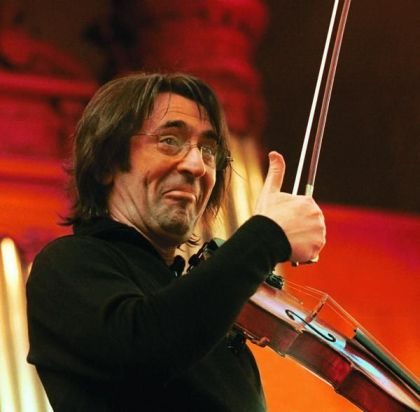
\includegraphics[width=4cm]{img/final/galat/petr.jpg}\vspace{-8pt}
   \end{wrapfigure}\textit{Как-то был на~конференции в~регионе, ну и в~рамках культурно-массовых
    вечерних мероприятий оказались на~концерте. 
    Кому-нибудь что-нибудь говорит здесь фамилия Башмет? в~общем, не так часто артистов такого уровня, как Башмет,
     можно встретить в~регионе. Ну вот ситуация: концертный зал, перед самой сценой сидит губернатор с~супругой.
      Проигрывается несколько произведений и супруга (жена губернатора) говорит: «обожаю, когда цыгане на~скрипке играют». 
      Вот и я~сейчас чувствую себя цыганом, скрипки правда у меня нет.}


\subsection{Функция действительной переменной}

Что значит $\lim\limits_{x\to a}f(x)\hm=l$ ? Напомню $(a,l\in \R)$ "--- принадлежат одной и той же числовой прямой.

Это значит:

\begin{Def}\label{Koshi} Предел функции по~Коши:

\begin{enumerate}
    \item $\exists\  \delta_0\hm>0\colon f(x)$ определена в~$B'_{\delta_0}(a)$ "--- проколотой окрестности точки $a$.

    \item $\forall\  \e\hm>0\ \exists\ \delta\hm>0\colon
    \underset{\substack{\dd \\ \text{удобнее} \\ \underset{\dd}{0\hm<}|x-a|\hm<\delta \\ \text{проколотая же}}}{\forall\  x\in B'_{\delta}(a)}
    \pau
    \underset{\substack{\text{удобнее} \\ |f(x)-l|\hm<\e}}{f(x)\in B_{\e}(l)}$ "--- совсем даже не проколотая окрестность.
\end{enumerate}

Эти помеченные удобства имеют место только тогда, когда предел конечен.

\end{Def}

\begin{Def}По Гейне.
    Для любых последовательностей точек $\big\{x_n\big\}_{n\hm=1}^{\infty}$, удовлетворяющих следующим условиям:

    \begin{enumerate}
        \item $f$ определена во всех точках $x_n$,

        \item $x_n\xrightarrow[n\to\infty]{} a$, но при этом $x_n\neq a$ ни для одного $n$;
    \end{enumerate}

Для любой такой разрешённой последовательности $x_n\pau f(x_n)\xrightarrow[n\to\infty]{}l$.
\end{Def}

Вместо $x_n\neq0$ можно записать $x_n\in\R\dd \{a\}$ "--- так будет удобнее.

Перед тем, как искать предел, надо понять, есть ли он вообще.

\subsection{Критерий Коши. Существование предела}
\begin{Def}
    Функция $f(x)$ удовлетворяет условию Коши в~точке $a\in\R$, если

    \begin{enumerate}
        \item $\exists\  \delta_0\hm>0\colon f(x)$ определена в~$B'_{\delta_0}(a)$ "---техническое ограничение;

        \item $\forall\ \e\hm>0\ \exists\ \delta\hm>0\colon\forall\  \tilde{x},\tilde{\tilde {x}}\in B'_\delta(a)\pau |f(\tilde x)-f(\tilde{\tilde x})|\hm<\e$.
    \end{enumerate}
\end{Def}

\begin{The}[Критерий существования предела функции] \label{KKoshi}
    

    $\lim\limits_{x\to a} f(x)$ существует и конечен $\hm{\iff}$ функция $f(x)$ удовлетворяет условию Коши в~точке~$a$.
\end{The}

\begin{Proof}
    Начнём с~тривиальной стороны:
    \begin{enumerate}
        \item Пусть $\lim\limits_{x\to a} f(x)\hm=l\in\R$.
            Зафиксируем произвольное $\e\hm>0$, для $\e_1\hm=\dfrac{\e}{2}$ из~предела найдём величину $\delta\hm>0\colon
            {\forall\  x\in B'_\delta(a) \pau |f(x)-l|\hm<\e_1}$.
            Тогда для любых точек $\tilde x,\tilde{\tilde x}\in B'_\delta(a)$ давайте посмотрим, как
            значения функции могут отличаться:
            $|f(\tilde x)-f(\tilde{\tilde x})|\hm=\underset{\text{(неравенство треугольников)}}{|f(\tilde x)-l+l-f(\tilde{\tilde x})|\leq |f(\tilde x)-l|+|l-f(\tilde{\tilde x})} |\hm<\e_1+\e_2\hm=\e$. Значит, функция удовлетворяет условию Коши в~точке $a$.

            в~тривиальную сторону критерий Коши всегда легко доказывать;

        \item В~этом случае удобнее оказывается определение по~Гейне: пусть $f(x)$ удовлетворяет условию Коши в~точке~$a$.
            Возьмём произвольную последовательность $\big\{x_n\big\}_{n\hm=1}^{\infty}$, удовлетворяющую ограничениям определения Гейне. Покажем, что тогда $\big\{f(x_n)\big\}_{n\hm=1}^\infty$ "--- фундаментальная последовательность.

            Ну, показываем: зафиксируем произвольное $\e\hm>0$. Найдём такую $\delta\hm>0\colon \forall\  \tilde x,\tilde{\tilde x}\in B'_\delta(a)\pau |f(\tilde x)-f(\tilde{\tilde x})|\hm<\e$.

            в~последовательности: найдём такой $\underset{(\text{используем }x_n\to a)}{\text{номер }N\text{, что }\forall\  n\hm>}N\ x_n\in B_\delta(a)$ "--- та же дельта, и все $x_n\neq a$.
            Значит, $\forall\  n\hm>N\pau x_n\in B'_\delta(a)$, тогда $\forall\  n,m\hm>N$ что можем сказать про отличие:  $|f(x_n)-f(x_m)|\hm<\e$.

            Забываем про лирику и смотрим, что мы написали: мы доказали фундаментальность последовательности. Значит, существует $\lim\limits_{n\to\infty}f(x_n)\hm=l\in\R$.

            Можно подумать, что уже доказали для функций, но это не так: мы взяли только одну последовательность точек. Осталось доказать, что для всех выборов $\big\{x_n\big\}_{n\hm=1}^\infty$ предел один и тот же.

            Докажем несколько изящным способом. Пусть $\big\{x_n\big\}_{n\hm=1}^\infty,\big\{\mathring{x}_n\big\}_{n\hm=1}^\infty$ "--- последовательности, удовлетворяющие ограничениям определения Гейне.
            Тогда $x_1,\mathring{x}_1,x_2,\mathring{x}_2,x_3,\mathring{x}_3,\ldots$ "--- также последовательность, удовлетворяющая ограничениям определения Гейне. Можем взять номер $N$ наибольший, на~два умножить на~всякий случай.
           Значит, существует конечный предел последовательности $f(x_1),f(\mathring{x}_1),f(x_2),f(\mathring{x}_2),\ldots$

            Осталось сказать: предел любой подпоследовательности ровно такой же предел, как и у последовательности, если она сходится: одинаковы пределы у $\big\{f(x_n)\big\}_{n\hm=1}^\infty$ и у последовательности $\big\{f(\mathring{x}_n)\big\}_{n\hm=1}^\infty$. Всё, критерий Коши доказан.



    \end{enumerate}
\end{Proof}

Следующая вещь, которую мы на~пальцах обсудим:

\subsection{Предел по~множеству}

\begin{Def}
    Пусть $A\subset \R$ и $\underset{a\in \ol{\R}}{a\text{ "--- преде}}$льная точка множества $A$. % Это шедевр. Я~долго смеялся. —А. В.—

    Предел $f(x)$ при $x\to a$ по~множеству $A$ равен $l\ (l\in\ol{\R})$.

    Начинаю делать для вас страшное: $\lim\limits_{A\ni x\to a} f(x)\hm=l$, если

    \begin{enumerate}
        \item $\exists\ \delta_0\hm>0\colon f(x)$ определена в~$B'_{\delta_0}(a)\cap A$;

        \item \begin{enumerate} \item $\forall\ \e\hm>0\ \exists\ \delta\hm>0\colon\forall\  x\in B'_\delta(a)\cap A\pau f(x)\in B_\e(l)$;

        \item $\forall$ последовательности точек $\big\{x_n\big\}_{n\hm=1}^\infty$, которая удовлетворяет условиям:

        \begin{enumerate}
            \item $f$ определена во всех $x_n$;

            \item $x_n\xrightarrow[n\to \infty]{}a\pau x_n\in A\dd\{a\},$

            $$f(x_n)\xrightarrow[n\to \infty]{}l.$$
        \end{enumerate}

        \end{enumerate}


    \end{enumerate}

    \end{Def}
    Все предыдущие утверждения работают.

    \subsection{Примерчик}

    Функция Дирихле "--- это такая вредная штука:

    \[
        D(x)\hm=\begin{cases}
        0,&x\in\R\dd\Q;\\
        1,&x\in \Q.
        \end{cases}
    \]

    $\lim\limits_{x\to a} D(x)$ "--- его просто нет.

    $\lim\limits_{\Q\ni x\to a} D(x)\hm=1$

    $\lim\limits_{(\R\dd \Q)\ni x\to a} D(x)\hm=0$

    $a$ должна быть предельной точкой, чтобы к~ней можно было подойти: если $a$ не предельная, то $\exists\  \delta\colon B'_\delta(a)\cap A\hm=\varnothing$, и тогда любое $l$, какое ни возьмём, будет являться пределом, так не интересно.

    Несложно видеть, что $\lim\limits_{x\to a}f(x)\hm=\lim\limits_{\R\ni x\to a}f(x)$ "--- могли вообще не обсуждать простой предел, а~сразу рассматривать предел по~некоторому множеству.

    \begin{Ut}\label{edprmn}
    Если $\lim\limits_{A\ni x\to a}f(x)$ существует, конечный или бесконечный, то он единственный.
            \end{Ut}

    \begin{Proof}
        Можно взять и честно доказать, а~можно свести к~последовательностям.

        Утверждение следует из~единственности предела последовательности и существования $\big\{x_n\big\}_{n\hm=1}^\infty$, удовлетворяющей ограничениям определения Гейне. Ну как строить последовательность: берём в~какой-то окрестности, входящей в~$A$, точку $x_1$ "--- какую-нибудь найдём, и можно дальше взять окрестность меньше раза так в~два, найдём там $x_2$ и т.\,д.

        Если бы у функции было два предела, то и у последовательности было два предела, а~это невозможно (утверждение \ref{edin}).
    \end{Proof}

    \begin{Ut}\label{mpod}
        Если $a$ "--- предельная точка $A$, $A\subset \tilde A$, $\exists\ \lim\limits_{\tilde A\ni x\to a}f(x)\hm=l\in\ol{\R}$, то $\exists\ 
        \lim\limits_{A\ni x\to a}f(x)\hm=l\in\ol{\R}$.
    \end{Ut}

    \begin{Proof}
    Если что-то верно для всех точек множества, то верно и для всех точек его подмножества.
    \end{Proof}

    \begin{Ut}
        Если $\exists\ \delta\hm>0\colon A\cap B'_\delta(a)\hm=\tilde A\cap B'_\delta(a),$ то $\lim\limits_{A\ni x\to a}f(x)$ и
        $\lim\limits_{\tilde A\ni x\to a}f(x)$ одновременно или не существуют, или равны.
    \end{Ut}

    \textbf{Введём ещё пару обозначений, с~которыми удобно работать.}

    \begin{Def}
        Пусть $a$ у меня пока конечное, то есть $a\in \R$, тогда $\lim\limits_{(-\infty,a)\ni x\to a}f(x)$ и
        $\lim\limits_{(a,+\infty)\ni x\to a}f(x)$ называются односторонними пределами (левым и правым) и обозначаются
        $\lim\limits_{\substack{x\to a- \\ \mathclap{\text{некоторые}} \\ \mathclap{\text{пишут}} \\ x\to a-0 }}f(x)$ и $\lim\limits_{x\to a+}f(x)$.

        $x$ стремится к~$a$, оставаясь меньше $a$.
    \end{Def}
        Что происходит при $a\hm=0$:\pau $0+0,\pau 0-0,\pau 0+,\pau+0$ "--- кто как ленится.

    Пусть функция $f(x)$ определена на~множестве $A$.
    \begin{Def}\label{vrost}
        $f(x)$ возрастает (иногда говорят, строго возрастает) на~$A$, если $\forall\  x_1,x_2\in A\ x_1\hm<x_2\hm{\imp} f(x_1)\hm<f(x_2)$.

        Обозначим $\nearrow$;

        Неубывает $f(x_1)\leq f(x_2) \ \nv$;

        Убывает $f(x_1)\hm>f(x_2)$ $\searrow$;

        Невозрастает (убывает в~нестрогом смысле) $f(x_1)\geq f(x_2)$ $\nuu$.

        Если функция $\searrow$ или $\nearrow$, то она называется строго монотонной на~$A$. Если функция $\searrow,\nearrow,\nuu$ или $\nv$, то она называется нестрого монотонной.
    \end{Def}

    а~если $a$ бесконечно, $\lim\limits_{x\to +\infty-0}$ "--- только левый предел, он же обычный.

    Можем взять и рассмотреть $\lim\limits_{\mathbb{N}\ni x\to+\infty}f(x)$, получим предел последовательности.

    \begin{Ut}\label{pmfq}
        Пусть функция $f(x)$ определена на~\textit{интервальчике} $(a,b)$ и неубывает. Тогда существует (конечный или бесконечный)
        $\lim\limits_{\substack{x\in b-0 \\ \mathclap{\text{(с разрешённой}} \\ \mathclap{\text{стороны)}}}}f(x)\hm=\sup\limits_{x\in(a,b)}f(x)$.
    \end{Ut}

    \begin{Proof}
        Обозначим $\sup\limits_{x\in(a,b)}f(x)\hm=s$ "--- либо конечный, либо $+\infty$.
        Возьмём произвольное $\e\hm>0$, найдём такую точку $x_0\in(a,b)$, что $f(x_0)\in B_\e(s)$ (рисунок \ref{pmf}).

        Найдём такую $\delta\hm>0$, что $B'_\delta(b)\cap(a,b)\subset(x_0,b)$\pau (\textit{букв много, а~смысла существенно меньше}).
        Можем взять $\delta\hm=b-x_0$, тогда $\forall\  x\in B'_\delta(b)\cap(a,b)$\pau
         $f(x_0)\leq f(x)\leq s\hm{\imp} f(x)$ тем более принадлежит $B_\e(s)$, тем самым мы доказали, что $s\hm=\lim\limits_{x\to b-0}f(x)$.

        \begin{figure}[htbp]\centering
    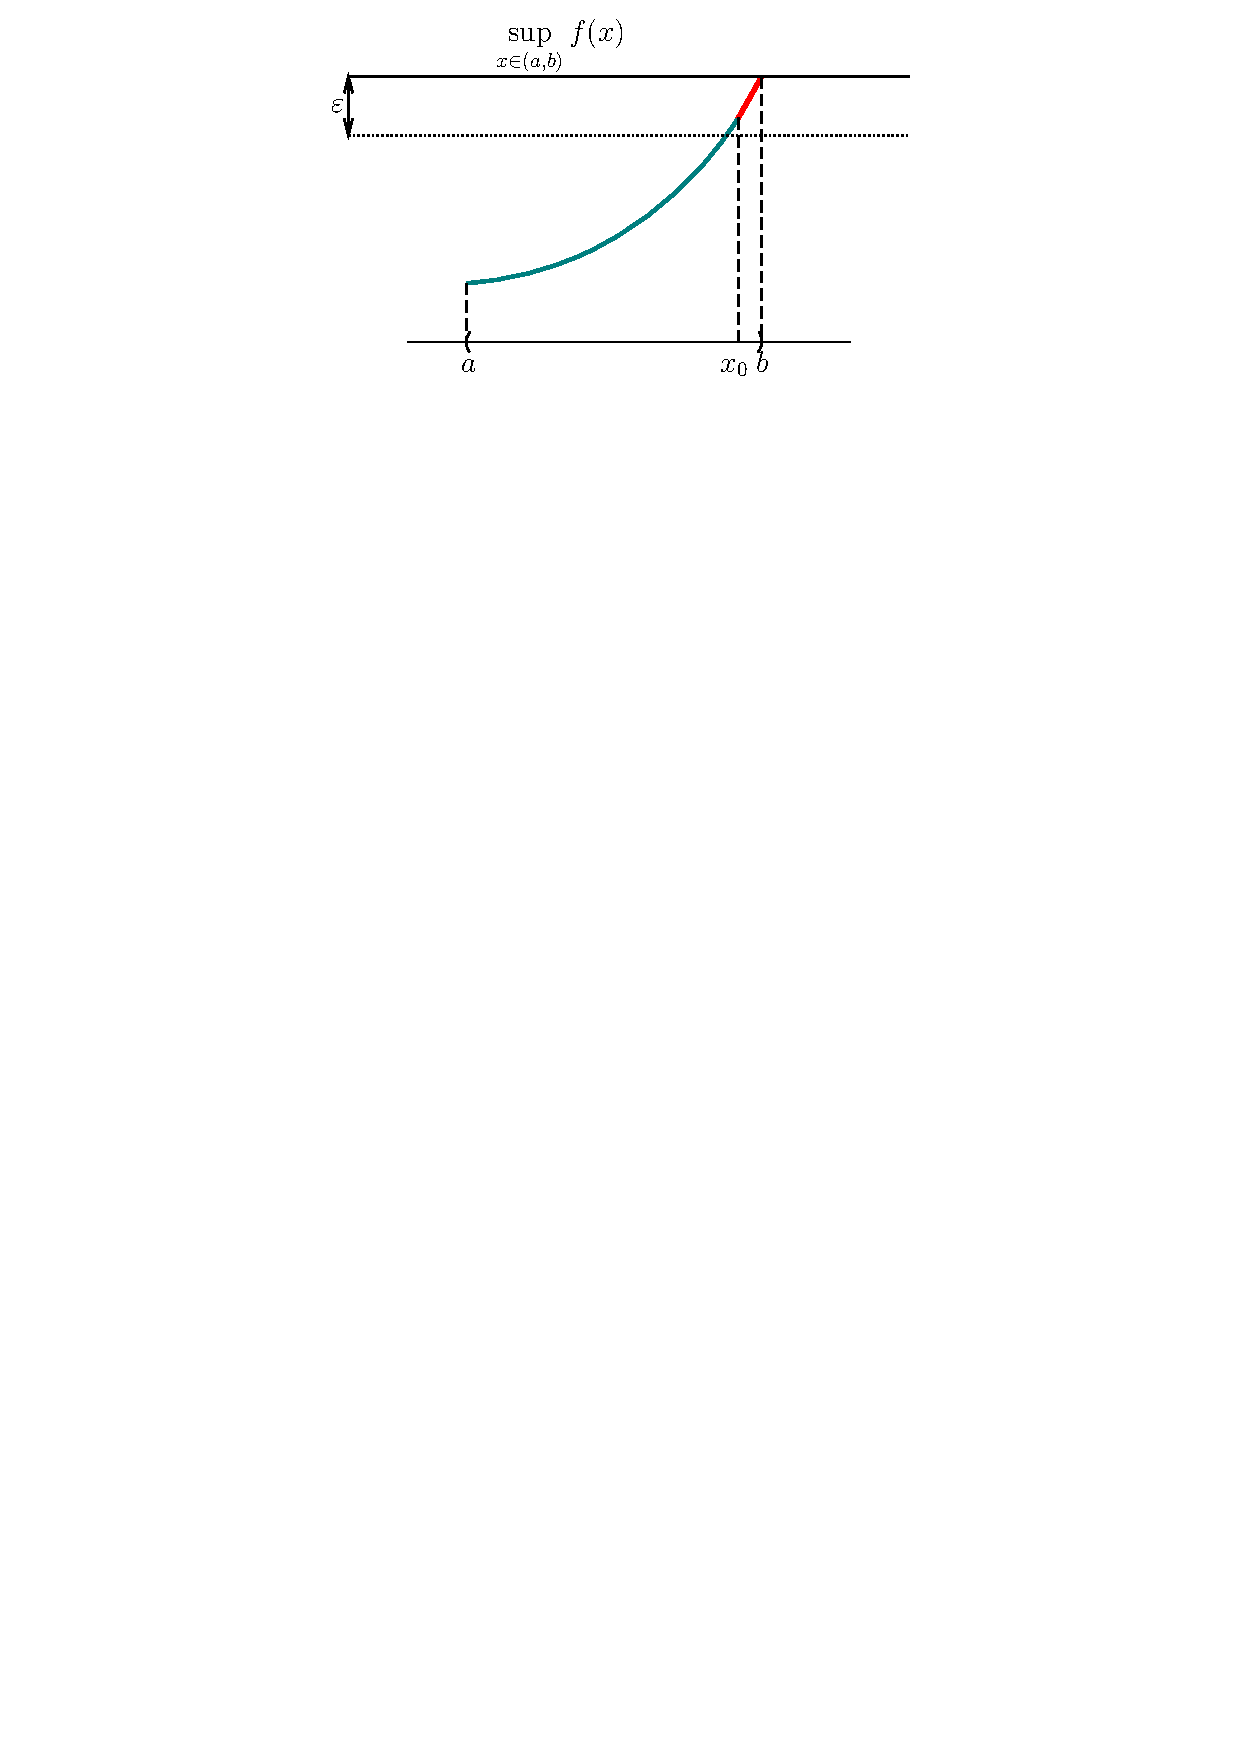
\includegraphics[width=9cm]{img/final/galat/funk.pdf}\caption{Предел монотонной функции}\label{pmf}
\end{figure}
    \end{Proof}


Зачем я~занимался фигнёй:
\begin{Zam}
Утверждение и доказательство верны для $(a,b)\subset\ol\R$. Ещё
\end{Zam}
\begin{enumerate}
\item  Если $f(x)\nuu$, то $\exists\  \lim\limits_{x\to b-0}f(x)\hm=\inf\limits_{x\in(a,b)}f(x)$. Можем идти и налево:

\item $f(x)\nv\hm{\imp}\lim\limits_{x\to a+0}f(x)\hm=\inf\limits_{(a,b)}f(x)$;

\item $f(x)\nuu\hm{\imp}\lim\limits_{x\to a+0}f(x)\hm=\sup\limits_{(a,b)}f(x)$;

\item Верны и аналоги этих утверждений, в~которых предел рассматривается по~множеству $A\subset(a,b)$. Ну естественно, если $a,b$ "--- предельные точки этого множества.

\end{enumerate}
$\lim\limits_{(a,b)\ni x\to a}f(x)\hm=\lim\limits_{x\to a+0}f(x)$.

Теперь можем $\lim\limits_{A\ni x\to a}f(x)\hm=\inf\limits_{x\in A}f(x)$.

Что если у нас $f(x)$ монотонна на~$(a,b)$, а~мы возьмём точку посередине. Предел слева и справа не обязан совпасть.

\begin{Ut}\label{rile}
Следующие утверждения эквивалентны:
\begin{enumerate}
    \item $\exists\ \lim\limits_{x\to a}f(x)\hm=l\in\ol{\R}$;
    \item $\lim\limits_{x\to a-}f(x)\hm=\lim\limits_{x\to a+}f(x)\hm=l$.
\end{enumerate}

\begin{Proof}
    в~одну сторону: если есть предел по~множеству, есть и по~подмножеству (утверждение \ref{mpod}). В~другую: возьмём меньшую из~дельт, она обслужит и левый и правый пределы.
   То есть: зафиксируем произвольное $\e\hm>0$. Найдём $\delta_1\hm>0\colon \forall\  x\in (a,a+\delta_1)\pau f(x)\in B_\e(l)$, найдём
   $\delta_2\hm>0\colon \forall\  x\in (a-\delta_2,a)\pau f(x)\in B_\e(l)$. Тогда $\forall\  x\in \big(a-\min\{\delta_1,\delta_2\},a+\min\{\delta_1,\delta_2\}\big)\pau
   f(x)\in B_\e(l)$.
\end{Proof}

\end{Ut}

\section{Непрерывность}

\subsection{Теорема о пределе композиции}
Ещё чуть-чуть про пределы, а~потом уже про непрерывность. Про технические ограничения я~больше говорить не буду.

$\lim\limits_{x\to a}f(x)\hm=b$ напомню означает $\forall\ \e\hm>0\pau \exists\ \delta\hm>0\colon x\in B'_\delta(a)\pau f(x)\in B_\e(b)$.

\begin{Ut}[Теорема о пределе композиции]\label{tpk}
Пусть $\lim\limits_{x\to a}f(x)\hm=b$, $\lim\limits_{y\to b}g(y)\hm=c$; $a$, $b$, $c$, вообще говоря,
 принадлежат расширенной числовой прямой: $a,b,c\in\ol{\R}$.

$\a$пустое место$\s$ "--- потом, когда мы придём к~дурным выводам, оно перестанет быть пустым.

Тогда куда же будет стремиться: $\lim\limits_{x\to a}g\big(f(x)\big)\hm=c$ "--- получалось, надо сказать, враньё. Почему:

Например: $g(y)\hm=\begin{cases}
    1,&y\neq0;\\
    0,&y\hm=0.
\end{cases}$ Пусть $f(x)\equiv 0$ "--- вообще тривиальная функция (рис. \ref{rkomp}).

$f(x)\xrightarrow[x\to 0]{}0$ тождественный ноль везде стремится к~нулю,     $g(y)\xrightarrow[y\to 0]{}1$, а~вот $g\big(f(x)\big)\equiv 0\xrightarrow[x\to 0]{}0$. Ну с~чем связаны все проблемы? на~внешнюю функцию никак не влияет значение $x\hm=a$.

\begin{figure}[htbp]\centering
    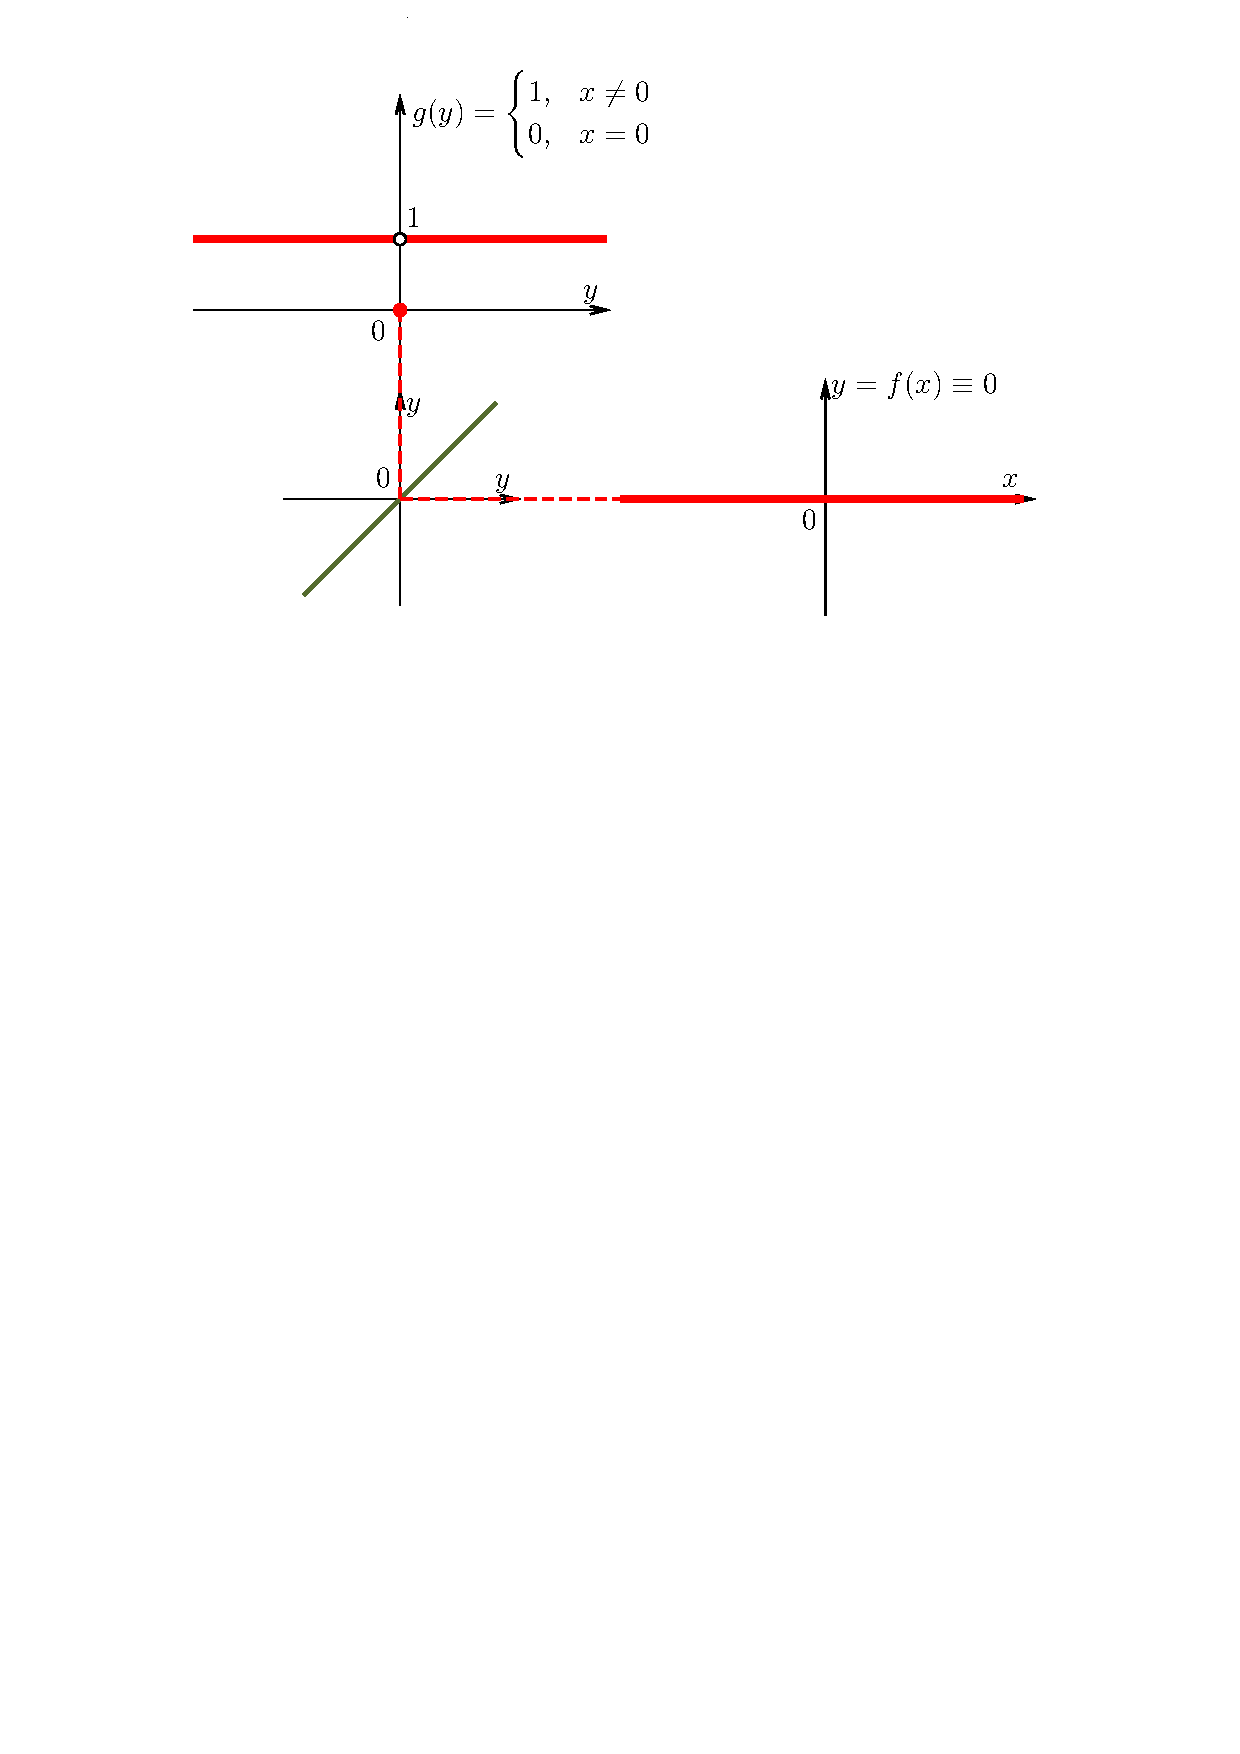
\includegraphics[height=6cm]{img/final/galat/vvedf/graf.pdf}\\ \caption{Разрывная композиция} \label{rkomp}
\end{figure}

Самое время в~$\a$пустое место$\s$ поставить: пусть выполняется хотя бы одно из~следующих утверждений:

\begin{enumerate}
    \item\label{a} $g(b)$ определена и равна $c$;
    \item\label{b} $f(x)$ не принимается значения $b$ в~некоторой проколотой окрестности $a$.
\end{enumerate}
\end{Ut}

Европеец в~главном здании какой-нибудь спрашивает, где корпус «бэ»? Что вот он имеет в~виду кириллическую Б или латинскую?

\begin{Proof}
Зафиксируем произвольное $\e\hm>0$, найдём $\delta\hm>0\colon \forall\  y\in B'_\delta(b)\pau g(y)\in B_\e(c)$. Найдём 
величину $\gamma\hm>0\colon \begin{cases}
    \forall\  x\in B'_\gamma(a);\\
    f(x)\in B_\delta(b).
\end{cases}$

Тогда $\forall\  x\in B'_\gamma(a)$ что можем сказать про величину $g\big(f(x)\big)$? Утверждаю, что $g\big(f(x)\big)\in B_\e(c)$. Почему это так?
В чём проблема, смотрите: $f(x)\in B_\delta(b)$ "--- непроколотая, $y\in B'_\delta(b)$ "--- проколотая.

Если выполнено \ref{a}, то тривиально: если $f(x)\in B'_\delta(b)$, то $g\big(f(x)\big)\in B_\e(c)$  в~силу выбора $\delta$.

Если же функция обратилась в~$b$: $f(x)\hm=b$, то $g\big(f(x)\big)\hm=g(b)\hm=c\in B_\e(c)$.

Если выполнено \ref{b}, то, быть может, сузив окрестность точки $a$, получим, что $f(x)$ принадлежит именно проколотой
$B'_\delta(b) \hm{\imp} g\big(f(x)\big)\in B_\e(c)$\footnote{
Зафиксируем $\e\hm>0$, найдём такую $\delta\hm>0$, что $\forall\  y\in B'_\delta(b)\pau g(y)\in B_\e(c)$, найдём такую
$\gamma_1\hm>0$, что $\forall\  x\in B'_{\gamma_1}(a)\pau |f(x)-b|\hm<\delta$, найдём такую $\gamma_2\hm>0$,
что $\forall\  x\in B'_{\gamma_2}(a)\pau f(x)\neq b$. Положим $\gamma\hm=\min\{\gamma_1,\gamma_2\}$, тогда $\forall\  x\in B'_\gamma(a)\pau
f(x)\in B'_\delta(b)$ и автоматически $\gf x\in B_\e(c)$.}.
\end{Proof}

\subsection{Непрерывность}
Следующее каноническое понятие в~математическом анализе "--- \textbf{непрерывность.}

\begin{Def}
Функция $f(x)$ называется непрерывной в~точке $a$, если она определена в~некоторой окрестности 
$a$ $\big(\exists\ \delta_0\colon f(x)$ определена в~$B_\delta(a)\big)$ и 
$\forall\ \e\hm>0\ \exists\ \delta\hm>0\colon \forall\  x\in B_\delta(a)\pau |f(x)-f(a)|\hm<\e$.
\end{Def}
В определении предела $x$ лежали в~проколотой окрестности, и замена её на~не являющуюся проколотой приводила к~плохим последствиям, а~вот тут ничего не поменяется если окрестность сделать проколотой.

Написано в~последнем определении по~сути вот что: $\lim\limits_{x\to a}f(x)\hm=f(a)$.

Ещё одно парное определение.

\begin{Def}
Функция называется непрерывной в~точке $a$ по~множеству $A$, если

\begin{enumerate}
    \item $\exists\  \delta_0\hm>0\colon f(x)$ определена в~$B_{\delta_0}(a)\cap A$ и
        в~самой точке $a$;

    \item $\forall\ \e\hm>0\pau\exists\ \delta\hm>0\colon \forall\  x\in B'_{\delta}(a)\cap A \pau |f(x)-f(a)|\hm<\e$, уже выясняли, что неважно: проколотая окрестность, не проколотая$\ldots$
\end{enumerate}

Почему необходимы оговорки? $a$ обязана являться предельной точкой $A$.

$\lim\limits_{A\ni x\to a}f(x)\hm=f(a)$.
\end{Def}

А давайте посмотрим, что будет, если $a$ не является предельной точкой. Тогда $\exists\  \delta\hm>0\colon B_\delta(a)\cap A\hm=\q$, для всех элементов этого множества верно всё что угодно.

То есть $\Biggl[$ \begin{tabular}{ll}
$a$ "--- предельная точка $A$,& $\lim\limits_{A\ni x\to a}f(x)\hm=f(a)$\\
$a$ "--- не предельная точка,& игнорируем
\end{tabular}

Буду всё писать для обычного предела, для предела по~множеству всё то же самое.

\begin{Ut}
Если $f(x)$ непрерывна в~точке (определение \ref{ot})\footnote{Вот он, единственный пока что недостаток этих лекций.}$a$, то $f(x)$ ограничена в~точке $a$ (локально ограничена, рис. \ref{pogr}).

\begin{figure}[htbp]\centering
    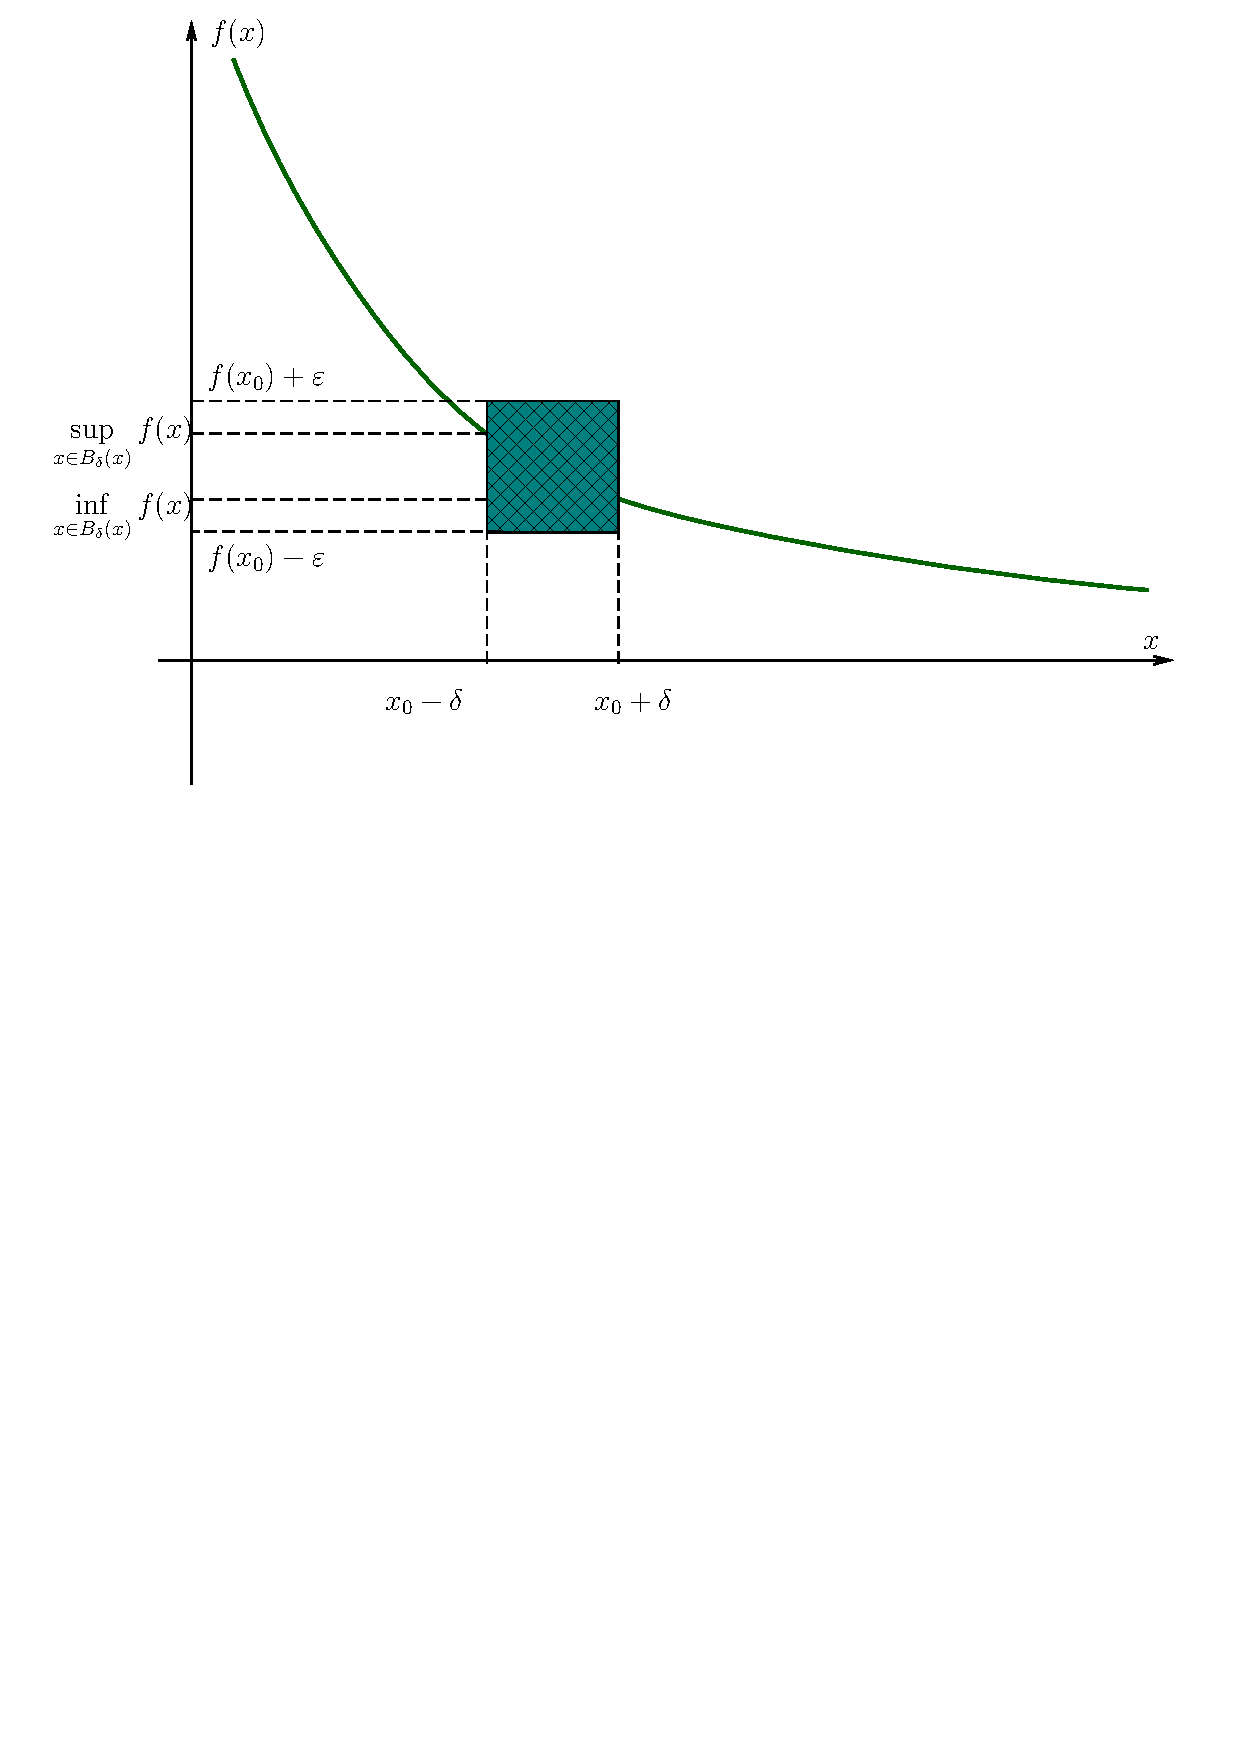
\includegraphics[height=8cm]{img/final/galat/ogr.pdf}\\ \caption{Непрерывна в~$x_0$ $\hm{\imp}$ ограниченна в~$x_0$}\label{pogr}
\end{figure}
\end{Ut}

Для общего развития головного мозга придумать пример функции, которая не ограничена ни на~одном отрезке.

\begin{Proof}
Положим $c\hm=|f(a)|+1$. Для $\e\hm=1$ найдём $\delta\hm>0\colon \forall\ 
x\in B_\delta(a)\pau |f(x)-f(a)|\hm<\e\hm=1$. Желающие вместо единицы могут поставить, что хотят. Тогда
$\forall\  x\in B_\delta(a)\pau |f(x)|\hm=|f(x)-f(a)+f(a)|\hm{\leq}|f(x)-f(a)|+|f(a)|\hm<1+|f(a)|\hm=c$.
\end{Proof}

\begin{Ut}\label{A2f}
Если $f(x)$ непрерывна в~точке $a$ и не обращается в~$0$, то существует окрестность точки $a$, в~которой $f$ сохраняет знак.
\end{Ut}

\begin{Proof}
Рассмотрим случай $f(a)\hm>0$. Для $\e\hm=\dfrac{f(a)}{2}$ найдём $\delta\hm>0\colon
\forall\  x\in B_\delta(a)\pau |f(x)-f(a)|\hm<\e$. Тогда $\underset{\hm=-\frac{f(a)}2}{-\e}\hm<f(x)-f(a)\hm<\underset{\hm=\frac{f(a)}{2}}{\e}$, прибавим $f(a)$. Во всей окрестности $\frac{f(a)}2\hm<f(x)$, а~$\frac{f(a)}2\hm>0$.

Тоже свойство техническое (как утверждение \ref{A2}):
\end{Proof}

\begin{Ut}
Пусть $f(x)$ и $g(x)$ непрерывны в~точке $a$, $\alpha\in\R$. Тогда
$\alpha f(x),\pau f(x)+g(x),\pau f(x)\cdot g(x)$ "--- непрерывны в~точке
$a$. Также если $g(0)\neq 0$, то $\frac{f(x)}{g(x)}$ непрерывна.
\end{Ut}
\begin{Proof}
Из одной строчки. Следует из~свойств предела функции и связи непрерывности и предела.
Если $f(x),g(x)$ определены в~некоторой окрестности , можем взять меньшую окрестность.

$\lim\limits_{x\to a}\big(f(x)g(x)\big)\hm=\lim\limits_{x\to a}f(x)\cdot \lim\limits_{x\to a}g(x)\hm=f(a)\cdot g(a)$, а~это значит, что произведение $f(x)g(x)$ в~точке $a$ непрерывно, остальные так же.
\end{Proof}

Ну и наверно последнее утверждение перед перерывом.

\begin{Ut}
Если $f(x)$ непрерывна в~точке $a$, $g(y)$ непрерывна в~точке $f(a)$, то $g\big(f(x)\big)$ непрерывна в~точке $a$.
\end{Ut}

\begin{Proof}
Следует из~сегодняшнего утверждения о пределе композиции. Определённость функции в~некоторой окрестности: $\exists\  \delta_0\colon g(y)$ определена в
$B_{\delta_0}\big(f(a)\big)$.

$\exists\  \gamma_0\hm>0\colon \forall\  x\in B_{\gamma_0}(a)
\pau |f(x)-f(a)|\hm<\delta_0$ (или по-другому записать: $f(x)\in
B_{\delta_0}\big(f(a)\big)$.
 Отсюда сразу следует, что $g\big(f(x)\big)$
определена в~$\gamma_0$ окрестности $a$. Выполнено условие \ref{a}.
$\lim\limits_{x\to a}
\tud{\gf x}{f(a)}\hm=\gf a$
    "--- и при этом в~самой точке эта композиция определена и принимает это значение.
\end{Proof}

Всё переносится на~пределы и непрерывность по~множеству.

\textit{Есть разные способы реагировать на~разные вещи. Был такой
 преподаватель, читал лекции, он считал, что перед его лекцией с
 доски обязательно должны стереть. Когда этого не случилось, в~качестве
 мести он стал писать поверх того, что уже написано. Между прочим, науке уже давно известны способы распознавать полезный сигнал при уровне шума во много раз более громкого, чем сам полезный
 сигнал. Я~могу взять уроки спортивного мужества у того преподавателя и читать
 лекцию поверх белого шума.}

Пусть $f(x)$ непрерывна в~точке $a$, определена во всех точках последовательности $\pos x$ и $x_n\te a$, тогда $f(x_n)\te f(a)$.


Что у нас произойдёт, если $x_i\hm=a$, $f(x_i)\hm=f(a)$. на~предел последовательности это никак не повлияет.

\begin{Def}
Функция $f(x)$ называется непрерывной на~множестве $A$, если она непрерывна в~$\forall\  a\in A$ по~множеству $A$.
\end{Def}

Зачем концовка этого определения: рисунок \ref{neopmno}.

\begin{figure}[htbp]\centering
    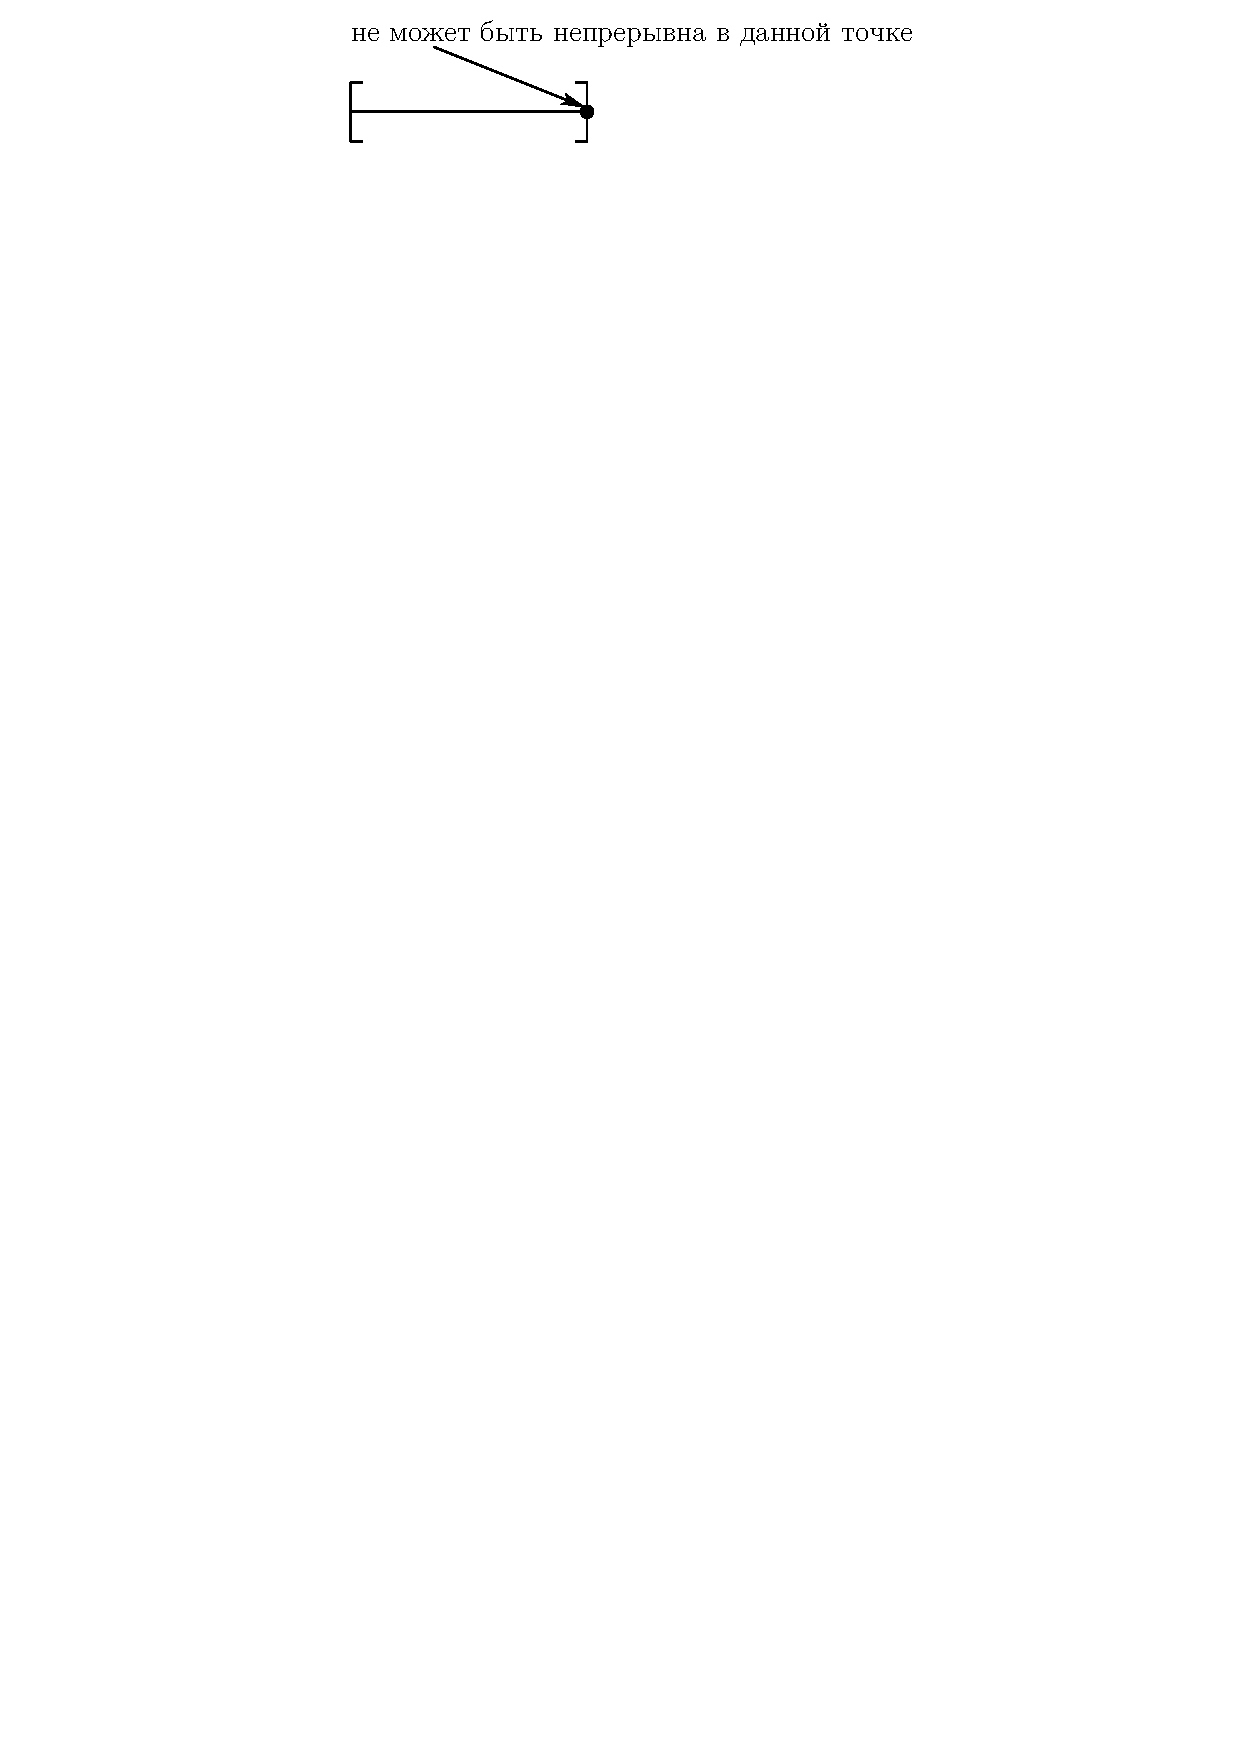
\includegraphics[height=1.5cm]{img/final/galat/nep.pdf}\\ \caption{Непрерывность на~множестве} \label{neopmno}
\end{figure}
$D(x)$ непрерывна на~$\Q$, на~$\R\dd\Q$ тоже непрерывна, а~на~$\R$ разрывна.

\begin{Def}
Подмножество $A$ действительной прямой называется промежутком, если
$\forall\  x,y\in A$ отрезок с~концами $x,y$ (не знаю, кто меньший) целиком лежит в~$A$.
\end{Def}

$\q$ "--- промежуток.

\begin{Ut}Пусть $A$ "--- непустой промежуток. Обозначу буковкой $i\hm=\inf A,\ s\hm=\sup A$(конечные или бесконечные). 
Тогда $(i,s)\subset A\subset[i,s]$.
\end{Ut}

\begin{Proof}
То, что $A\subset[i,s]$ тривиально из~определений \ref{Dsup} верхних и нижних граней. Осталось доказать, что $(i,s)\subset A$.

Пусть $t$ "--- произвольная точка интервала $(i,s)\hm{\imp} \exists\  x\in A\colon
x\hm<t$ (иначе было бы $t\hm=\inf A$), $\exists\  y\in A\colon y\hm>t$. По~определению промежутка $[x,y]\subset A$, а~мы взяли
\textbf{произвольную} точку из~интервала $(i,s)\ni t\hm{\imp} (i,s)\subset[x,y]\hm{\imp} (i,s)\subset A$.
\end{Proof}

 \begin{tabular}{|c|c|c|}
 \hline
        & $\q$      &вырожденные\\ \cline{2-2}
        &$\{a\}$    &промежутки\\ \hline
        &$(a,b)$    &           \\ \cline{2-2}
Ограниченные&$[a,b]$    & \\ \cline{2-2}
        &$(a,b]$    & \\ \cline{2-2}
        &$[a,b)$    & \\ \cline{1-2}
        &$(-\infty,a)$ снизу& невырожденные \\ \cline{2-2}
        &$(-\infty,a]$ снизу& \\ \cline{2-2}
Неограниченные&$(0,+\infty)$ сверху& \\ \cline{2-2}
        &$[a,+\infty)$ сверху& \\ \cline{2-2}
        &$(-\infty,+\infty)$& \\ \hline

\end{tabular}

При этом великий могучий русский язык проявляет себя в~полной мере.
Есть слова: интервал, отрезок, полуотрезок. 
В~статьях обычно выбирают только одно слово и обозначают им все промежутки, чаще всего это слово сегмент. 
В~зарубежных статьях промежутки отличаются эпитетами (open segment,$\ldots$).

\begin{Th}
Пусть функция $f$ непрерывна на~$[a,b]$, $f(a),\ f(b)$ имеют разные знаки. Тогда $\exists\  x_0\in[a,b]\colon
f(x_0)\hm=0$.
\end{Th}

\begin{Proof}
Метод деления отрезка пополам. Для определённости будем считать, что $f(a)\hm<0,\ f(b)\hm>0$. Положим $x_1\hm=a,\pau y_1\hm=b,\pau \Delta_1\hm=[a,b]$. Если в~середине отрезка $\Delta_1\pau f(x)\hm=0$, то искомую точку уже нашли. Если же не нашли, то в~качестве отрезка $\Delta_2$ возьмём ту половину $\Delta_1$, в
концах которой функция принимает значения разных знаков, в~качестве $x_2$ возьмём левый конец $\Delta_2$, в~качестве $y_2$ "--- правый.
И так далее.

Получим один из~двух вариантов: если на~$n$-ом шаге процесс закончился, тогда $x_0$ найдена.
В противном случае построена последовательность вложенных отрезков с~длинами стремящимися к~нулю. Тогда по~принципу полноты Кантора (теорема \ref{ppk}) у отрезков есть общая точка, которую я~обозначу через $x_0$.

Имеем, ну, во-первых, $f(x_n)\hm<0$ и $f(x_n)\te0$, почему это так?
    $$
    \overbrace{x_0-\tud{|\Delta_n|}{0}}^{\begin{smallmatrix}x_0\\ \uparrow\end{smallmatrix}}\leq x_n\leq x_0\leq y_n\leq
    \overbrace{x_0+\tud{|\Delta_n|}{0}}^{\begin{smallmatrix}x_0\\ \uparrow \end{smallmatrix}}.
$$
По лемме \ref{lzp} о зажатой последовательности $x_n\te x_0$.

$f(x_n)\te f(x_0)\hm{\imp}(x_0)\leq0$, аналогично $f(y_n)\te f(x_0)\hm{\imp} f(x_0)\geq0\hm{\imp} f(x_0)\hm=0$.
\end{Proof}

Это обосновывает метод интервалов.

\section{Свойства непрерывных функций. Равномерная непрерывность}
Пусть $I$ "--- промежуток (невырожденный). Что значит $f$ непрерывна на~$I$: она непрерывна в~каждой точке~$I$:
$\forall\  x_0\in I,\ \forall\ \e\hm>0\pau \exists\  \delta\hm>0\colon
\forall\  x\in B_\delta(x_0)\cap I\pau |f(x)-f(x_0)|\hm<\e$.
 Обозначение будем использовать вот такое: $f\in C(I)$.

Уже успели доказать: пусть $f\in C\big([a,b]\big),\pau f(a)$ и $f(b)$ имеют разные знаки,
тогда $\exists\  x_0\in [a,b]\colon f(x_0)\hm=0$.

Из этого утверждения немедленно следует:

\begin{The}[Больцано"--~Коши]\label{bk}
Непрерывная на~промежутке функция принимает все промежуточные значения.

Конкретизация: пусть $f\in C(I),\pau I$ "--- невырожденный промежуток, пусть $f$ принимает значения $A$ и $B$, то есть
$\exists\  a,b\in I\colon f(a)\hm=A$, $f(b)\hm=B$. Тогда $f$ примет (хоть один раз) промежуточное значение $C$, то есть $\exists\  c\in I\colon
f(c)\hm=C$.

\end{The}

Давайте её быстренько докажем.
\begin{Proof}
Рассмотрим функцию $g(x)\hm=f(x)-C$ "--- непрерывную на~всём промежутке $I$, а~значит и непрерывную на~отрезке c концами $a,b$ (пишу так, потому что не знаю, кто больше, $a$ больше, $b$ больше).

$\left.\begin{matrix}
g(a)\hm=A-C\\
g(b)\hm=B-C
\end{matrix}\right\}$ "--- значения разных знаков.

Значит, по~только что доказанной лемме в~отрезке с~концами $a,b\pau \exists\  c\colon g(c)\hm=0\hm{\imp} f(c)\hm=g(c)+C\hm=C$.
\end{Proof}

Вот такая простая теорема.

\begin{The}[Вейерштрасса об ограниченности функции на~отрезке]\label{vogr}
Пусть $f\in C\big([a,b]\big)$, тогда $f$ ограничена на~$[a,b]$, то есть $\exists\  C\hm>0\colon \forall\  x\in[a,b]\pau |f(x)|\leq C$.
\end{The}

\begin{Proof}
\begin{enumerate}
    \item От противного. Пусть $f\in C\big([a,b]\big)$ и $f$ неограниченна на~$[a,b]$ сверху (снизу будет аналогично).
    Так как $f$ неограничена сверху, то $\exists\  x_1\in [a,b]\colon f(x_1)\hm>1$, иначе $f$ ограничена единицей.
    $\exists\  x_2\in[a,b]\colon f(x_2)\hm>2$, $\ldots,\exists\  x_n\in[a,b]\colon
        f(x_n)\hm>n,\ldots$

        Что мы получили: $\pos x$ "--- ограниченная последовательность (ведь все её элементы были взяты из~отрезка). Значит,
        по~теореме \ref{b-v} Больцано"--~Вейерштрасса из~$\pos x$
        можно выделить сходящуюся подпоследовательность
        $\Big\{x_{n_k}\Big\}_{k\hm=1}^\infty$. Обозначим предел этой подпоследовательности за $x_0$: $x_{n_k}\tend{k\to\infty}x_0$. Точка $x_0\in [a,b]$,
        $\tud aa\leq\tud{x_{n_k}}{x_0}\leq\tud bb$ (утверждение \ref{pernes}). Так как $f$ непрерывна в~точке $x_0\pau f(x_{n_k})\to f(x_0)$.
         Это противоречит тому, что $\Big\{f(x_{n_k})\Big\}_{n\hm=1}^\infty$ хотите "--- неограниченная, хотите $\to\infty$;

        \item Просто так ещё один способ доказать эту теорему: $\forall\  x\in [a,b]\pau \exists\  \delta_x\hm>0\colon
            f$ ограничена на~$(x-\delta_x,x+\delta_x)\cap[a,b]$.
            Система интервалов
            $\Big\{(x-\delta_x,x+\delta_x)\Big\}_{x\in[a,b]}$ образует открытое покрытие $[a,b]$.
            Выделим из~этого покрытия конечное подпокрытие. Пусть оно состоит из~интервалов, соответствующих точкам $x_1,\ldots,x_N$. Пусть
            $C\hm=\max\{C_{x_1},C_{x_2},\ldots,C_{x_N}\}$. Тогда $f$ ограничена на~$[a,b]$ константой $C$.

            Отрезок можно заменить на~произвольный компакт.
\end{enumerate}
\end{Proof}

\begin{The}[Вейерштрасса]\label{vmaxmin} Непрерывная на~отрезке функция принимает свои наибольшее и наименьшее значение.


\pic{galat/19/fuq}{3}{fuq}{Непрерывная только на~интервалах функция}
На рисунке \ref{fuq} функция непрерывна только на~интервалах, нет
  ни самого маленького, ни самого большого значения.

$f\in[a,b],\pau \exists\  x_{\min},x_{\max}\in[a,b]\colon
\forall\  x\in[a,b]\pau f(x_{\min})\leq f(x)\leq f(x_{\max})$.
\end{The}

Раз  уж у нас сегодня идёт раздолбайство, докажем двумя способами.

\begin{Proof}
\begin{enumerate}
\item Для $\max$: пусть $f\in C\big([a,b]\big),\pau
M\hm=\sup\limits_{x\in[a,b]}f(x)\hm<+\infty$ (в силу уже доказанной теоремы \ref{vogr} Вейерштрасса).

\begin{tabular}{ll}
$\exists\  x_1\in[a,b]\colon$&$f(x_1)\hm>M-1$\\
$\exists\  x_2\in[a,b]\colon$&$f(x_2)\hm>M-\frac12$\\
$\vdots$\\
$\exists\  x_n\in[a,b]\colon$&$f(x_n)\hm>M-\frac1n$\\ $\vdots$
\end{tabular}

Куда же стремится $f(x_n)\te M$, так как $M-\frac1n\hm<f(x_n)\leq M$, дальше лемма \ref{lzp} о зажатой последовательности.

Теперь повторим то, что уже говорили: $\pos x$ "--- ограниченная последовательность,
выделим из~неё сходящуюся подпоследовательность $x_{n_k}$ (теорема \ref{b-v}), предел которой обозначим $x_0\in[a,b]$.
Что же мы имеем: $f(x_{n_k})\tend{k\to \infty}f(x_0)$, так как $f$ непрерывна в~точке $x_0$. С~другой стороны $f(x_{n_k})\to M$.
 В~силу единственности предела (утверждение \ref{edprmn}) $f(x_0)\hm=M$;

\item По~заявкам, не знаю уже насколько, трудящихся. Пусть $f\in\big([a,b]\big),\pau m\hm=\inf\limits_{x\in[a,b]}f(x)$.
    Предположим, что $f$ не принимает на~$[a,b]$ значение $m$, то есть $f(x)\hm>m$ на~$[a,b]$. Рассмотрим $g(x)\hm=\dfrac1{f(x)-m}$. Мораль: $g(x)\in C\big([a,b]\big)$.
    Значит, (теорема \ref{vogr} Вейерштрасса) ограничена на~$[a,b]$, то есть
    $\exists\  C\hm>0\colon g(x)\leq C$ на~$[a,b]$.

    $\dfrac{1}{f(x)-m}$ не превосходит $C\hm{\imp} f(x)-m\geq\dfrac1C\hm{\imp} f(x)\geq m+\dfrac1C$ "--- противоречие с~тем, что $m$ есть точная нижняя грань.

\end{enumerate}
\end{Proof}
\begin{Zam}
 Отрезок в~этой теореме может быть заменён на~произвольный компакт (например множество Кантора).
\end{Zam}
Важная на~самом деле штука. Вернёмся к~определению непрерывности.

Пусть $A$ "--- какое-то множество и  $f$ непрерывна на~$A\ \big(f\in C(A)\big)$. $\forall\  \tilde x\in A,\ \forall\ \e\hm>0\pau \exists\ \delta\hm>0\colon
\forall\  x\in A\colon |x-\tilde x|$ $|f(x)-f(\tilde x)|\hm<\e$

\pic{galat/19/rav}{4.5}{rav}{Равномерная непрерывность}

 Насколько мы можем ошибаться в~аргументе?

\begin{Def}
Функция $f$ равномерно непрерывна, если $f$ определена на~$A$ (ну так, на~всякий случай) и
$\forall\  \e\hm>0\pau \exists\  \delta\hm>0\colon
\forall\  x,\tilde x\in A\colon |x-\tilde x|\hm<\delta\pau |f(x)-f(\tilde x)|\hm<\e$.
\end{Def}

Теперь $\delta$ выбираем независимо от $\tilde x$. Часть утверждения «$\forall\  \tilde x\in A$» переехала вправо, кстати.

\begin{Zam} Если $f$ "--- равномерно непрерывна на~$A$, то, конечно, она просто непрерывна на~$A$.
\end{Zam}
\begin{Zam} Функция $x^2$ не является равномерно непрерывной на~$\R$, $\frac1x$ не является равномерно непрерывной на~$(0,1)$
. Конструктивно построил не равномерно непрерывную функцию.
\end{Zam}
\begin{Proof}\big[$f(x)\hm=x^2$\big] Покажем, что $\exists\  \e\hm>0\colon \forall\ \delta\hm>0\pau
\exists\  x,\tilde x\in A\colon |x-\tilde x|\hm<\delta\pau
|f(x)-f(\tilde x)|\geq \e$.

Пусть $\e\hm=1$. Для $\forall\  \delta\hm>0$ положим $x\hm=\dfrac1{\delta}$, а~$\tilde x\hm=\dfrac1{\delta}+\dfrac{\delta}2$, тогда $|x-\tilde x|\hm=\dfrac{\delta}2\hm<\delta\qquad |f(x)-f(\tilde x)|\hm=1+\dfrac{\delta^2}4\hm>\e$
\end{Proof}

\begin{The}[Кантора, реже Гейне, Кантора"--~Гейне, Гейне"--~Кантора]\label{kg}
Непрерывная на~отрезке функция равномерно непрерывна на~нём (отрезок можно заменить на~произвольный компакт).
\end{The}

\begin{Proof}
От противного: пусть функция $f\in C\big([a,b]\big)$, но $f$ не равномерно непрерывна на~$[a,b]$. Тогда
${\exists\  \e\hm>0\colon} {\forall\  \delta\hm>0}\pau
\exists\  x,\tilde x\in [a,b]\colon |x-\tilde x|\hm<\delta\pau |f(x)-f(\tilde x)|\geq \e$;

Для $\delta_1\hm=1\pau \exists\  x_1,\tilde x_1\in [a,b]\colon
|x_1-\tilde x_1|\hm<1\pau |f(x_1)-f(\tilde x_1)|\geq\e$;

Для $\delta_2\hm=\frac12\pau \exists\  x_2,\tilde x_2\in [a,b]\colon
|x_2-\tilde x_2|\hm<\frac12\pau |f(x_2)-f(\tilde x_2)|\geq\e$;

Для $\delta_n\hm=\frac1n$ найдутся $x_n,\tilde x_n\in [a,b]\colon
|x_n-\tilde x_n|\hm<\frac1n$, а~при этом $|f(x_n)-f(\tilde x_n)|\geq\e$ "--- по~крайней мере эпсилон.

Эти вещи зажаты: $\tud{-\frac1n}0\hm<x_n-\tilde x_n\hm<\tud{\frac1n}{0}\hm{\imp} x_n-\tilde x_n\te0$.

Из $\pos x$ выделим сходящуюся подпоследовательность $\Big\{x_{n_k}\Big\}_{k\hm=1}^\infty$ (теорема \ref{b-v}). Её предел обозначим через $x_0$, а~$x_0\in[a,b]$.

Тогда $\tilde x_{n_k}\hm=\tud{x_{n_k}}{x_0}+\tud{(\tilde x_{n_k}-x_{n_k})}{0}\xrightarrow[\text{мораль}]{n\to \infty}x_0\hm{\imp} 
f(x_{n_k})\tend{k\to \infty}f(x_0)$. $f(\tilde x_{n_k})\tend{k\to\infty}f(x_0)$, 
так как $f$ непрерывна в~точке $x_0\hm{\imp} \big(f(x_{n_k})-f(\tilde x_{n_k})\big)\tend{k\to\infty}0$. 
Это противоречит тому, что $\forall\  k\pau \big|f(x_{n_k})-f(x_{n_k})\big|\geq\e$.

\end{Proof}

За этим можно искать разные метознания. Простая непрерывность "--- свойство локальное,
равномерная непрерывность "--- свойство глобальное.
Локально $x^2$ равномерно непрерывен, глобально же свойство теряется. Около любого человека никто не конфликтует. Так вроде посмотришь вокруг и правда, а~глобально это, конечно, неверно.

\begin{The}
    Пусть $f$ "--- монотонная на~промежутке функция. Она непрерывна на~нём, если и только если она принимает на~этом промежутке все промежуточные значения.
\end{The}

\begin{Proof}
    Непрерывна $\hm{\imp}$ принимает все промежуточные значения (теорема \ref{bk}).

    Пусть $f\nv$ на~$I$ и принимает все промежуточные значения на~$I$, докажем, что $f\in C(I)$. Пусть $x_0\in I\colon$ не правый конец
    $I$, чтобы попроще. Пусть $x_1\in I\colon x_1\hm>x_0$. Тогда
    $\lim\limits_{x\to x_0+0}f(x)\overset{\ref{pmfq}}{\hm=}\inf\limits_{(x_0,x_1)}f(x)\hm=f(x_0)$, так как принимает все промежуточные значения.

    Аналогично $\lim\limits_{x\to x_0-0}f(x)\hm=f(x_0)\hm{\imp} \lim\limits_{x\to x_0}f(x)\hm=f(x_0)$
\end{Proof}

\section{Разрывы. Модуль непрерывности}

Давайте начнём. Начнём с~каких-то разрозненных кусков. Рассмотри функции совсем плохие, потом совсем хорошие и всё-таки вернёмся к~таким нормальным.

\subsection{Классификация точек разрыва}

\begin{Def}
    Точка $x_0\in\R$ называется изолированной точкой разрыва функции $f$, если для некоторого $\delta\hm>0$ функция $f$  непрерывна в~$B'_\delta(x_0)$, но разрывна в~точке $x_0$ (по каким-то причинам не является непрерывной в~точке $x_0$).
\end{Def}

Дальнейшая классификация относится, вообще говоря, к~изолированным точкам разрыва.

Рассмотрим два односторонних предела $\lim\limits_{x\to x_0+0}f(x)$ и $\lim\limits_{x\to x_0-0}f(x)$. Какие возникают варианты? Ну давайте я~начну с~самых таких плохих вариантов.
\begin{itemize}
\item[2.] Хотя бы один из~односторонних пределов не существует или бесконечен. Тогда разрыв называют \textbf{разрывом второго рода.} Если хоть один из~односторонних пределов бесконечен, то разрыв иногда называют бесконечным;


\begin{figure}[htbp]
\centering
\begin{minipage}{0.45\textwidth}
\centering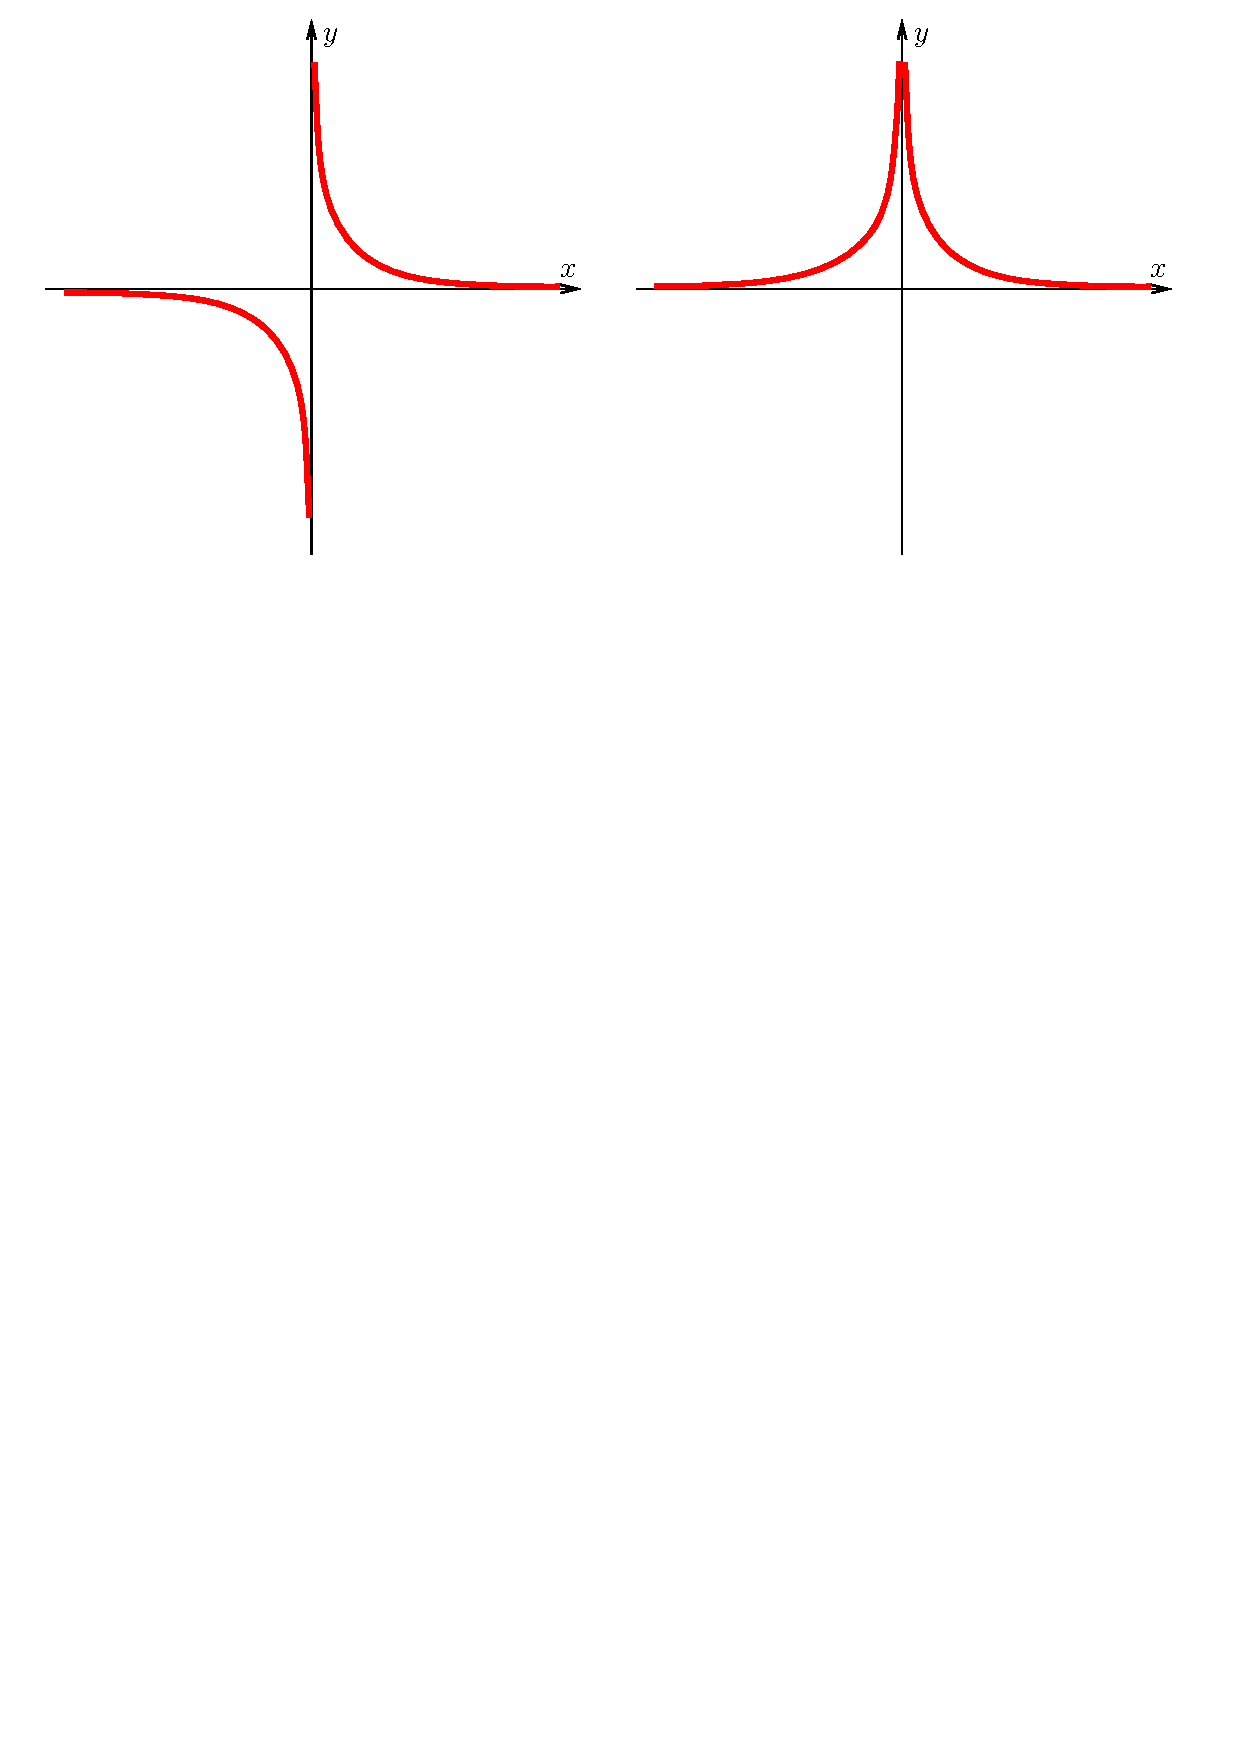
\includegraphics[width=80mm]{img/final/galat/20/1x1x2.pdf}
\caption{Какие нибудь $\frac1x$ и $\frac1{x^2}$}
\end{minipage}\qquad
\begin{minipage}{0.45\textwidth}
\centering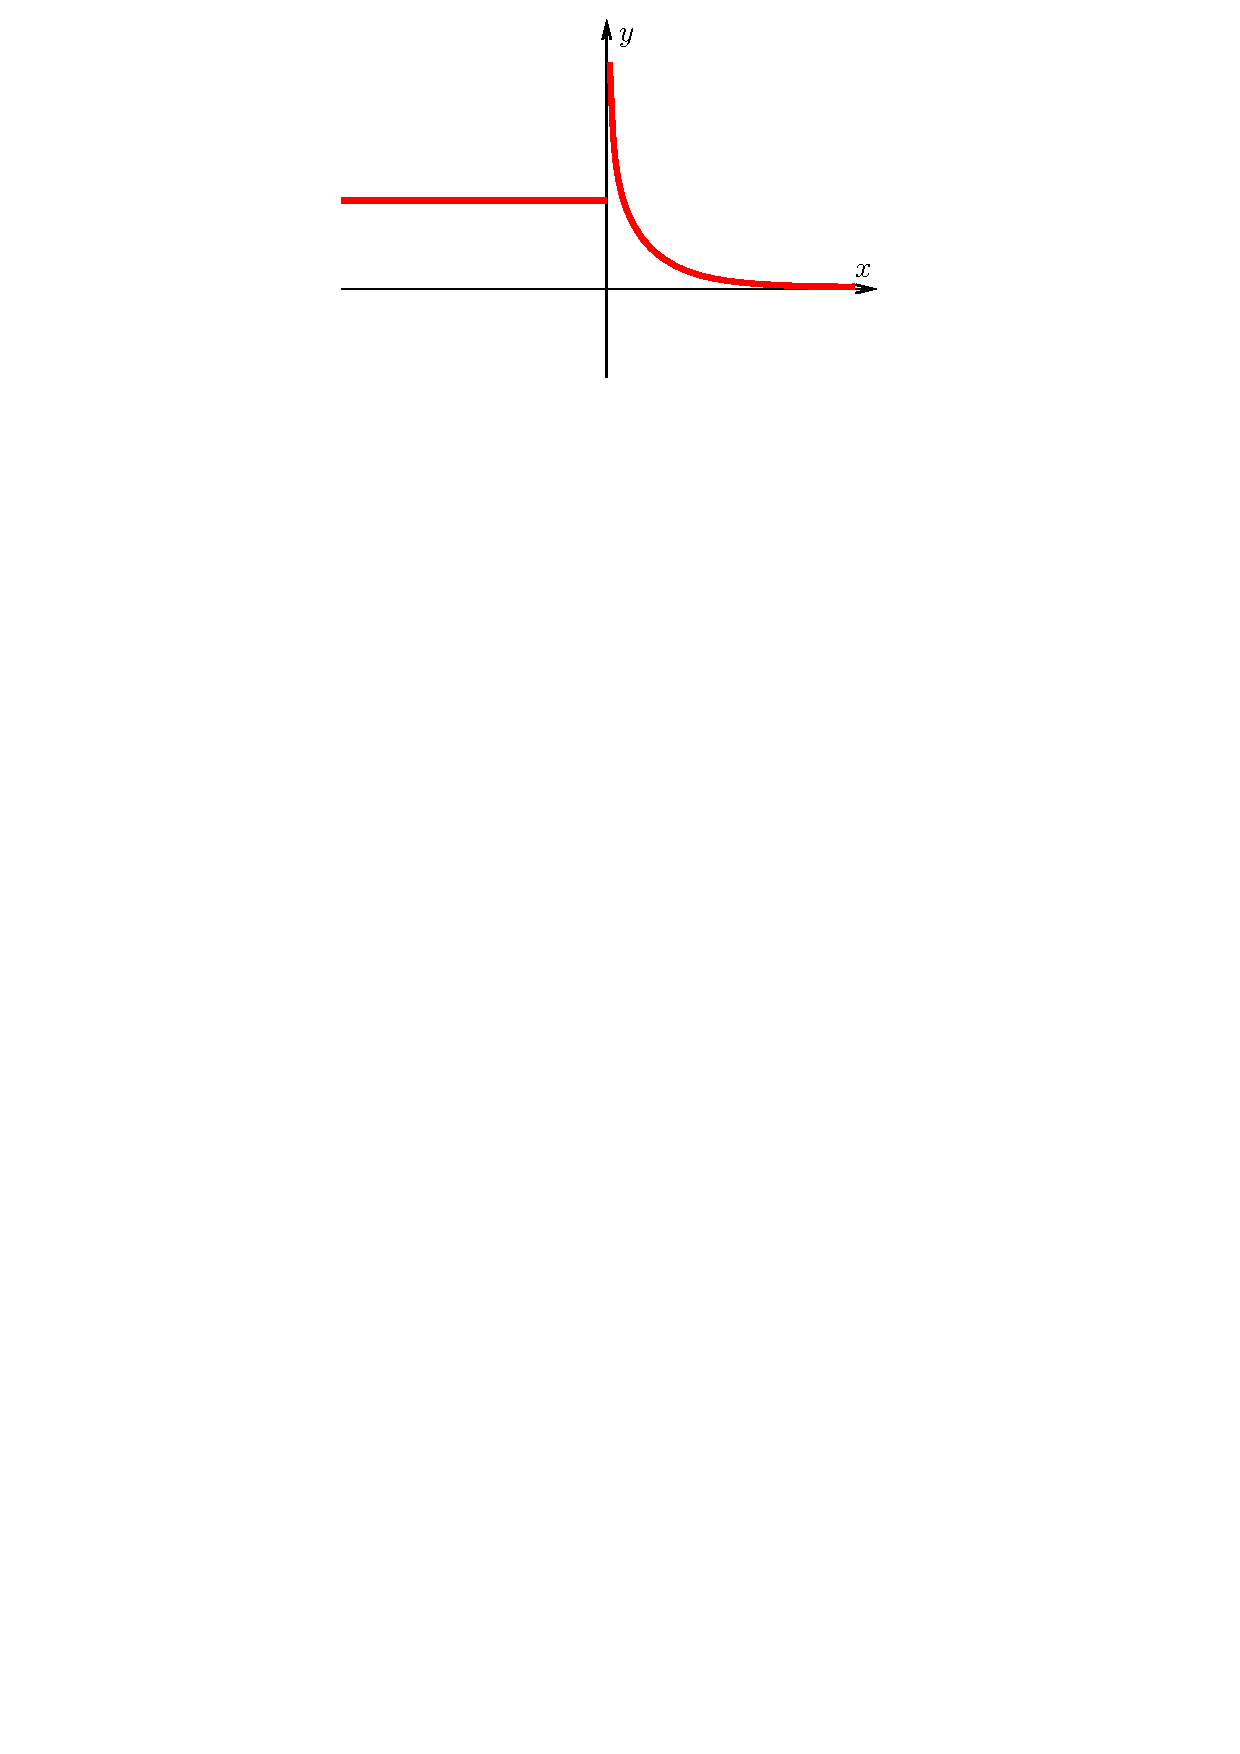
\includegraphics[width=50mm]{img/final/galat/20/vc.pdf}
\caption{Можем рассмотреть и такой случай}
\end{minipage}
\end{figure}



%\pic{galat/20/1x1x2}{4}{1x1x2}{Какие нибудь $\frac1x$ и $\frac1{x^2}$}
%\pic{galat/20/vc}{4}{vooc}{Можем рассмотреть и такой случай}

А какие есть примеры, где разрыв второго рода, который не является бесконечным: $\sin\left(\frac1x\right)$.


\item[1.] Оба односторонних предела существуют, конечны, но (чтобы не всё идеально было) не равны друг другу. Такой разрыв называют \textbf{разрывом первого рода};

\pic{galat/Rasr/r1r}{4}{r1r}{Скажем, $\mathrm{sgn}x$, он же $\dfrac{|x|}{x}$}

И совсем всё хорошо:

\item[0.] Оба односторонних предела существуют, конечны и равны друг другу (на всякий случай уточню: при этом значение $f(x_0)$ не определено
или отлично от значения односторонних пределов). Такой разрыв называют устранимым. Иногда устранимый разрыв относят к~разрывам первого рода, иногда нет.
В качестве примера возьмём какой-нибудь $\dfrac{\sin x}{x}$, в~точке $x_0\hm=0$ такая функция неопределена. Можем получить устранимый разрыв.

\begin{Ut}
Если $x_0$ "--- точка устранимого разрыва функции $f$, то функцию $f$ в~точке $x_0$ можно либо доопределить, либо переопределить так, что она станет непрерывной в~точке $x_0$.
\end{Ut}

Для разрывов других видов аналогичное утверждение неверно.

\end{itemize}

Как я~уже говорил: мы здесь говорим об изолированных точках разрыва. Поэтому ответ на~вопрос «какие разрывы у функции Дирихле?» «да никаких!» Если
изолированность убрать, то в~функции Дирихле были бы разрывы второго рода. $\ln x$ левее нуля не определён, поэтому, зачеркнув слово «изолированный»,
 получим разрыв второго рода.

 Обсудим, какие бывают у функции проблемы.

 Пока я~стираю "--- стандартный комментарий: антонимом к~слову «непрерывный» является «разрывный». Используемый часто студентами «прерывный» стандартным не является.

\subsection{Модуль непрерывности.}
 Давайте повторим:

 \begin{Def}\label{ravnep}
Функция $f$ называется равномерно непрерывной на~$A$, если она определена на~$A$ и $\forall\ \e\hm>0\pau
\exists\  \delta\hm>0\colon \forall\  x,\tilde x\in A\pau |x-\tilde x|\hm<\delta\pau |f(x)-f(\tilde x)|\hm<\e$.
 \end{Def}

 Пока не связанное с~верхним определение:

 \begin{Def}
 Пусть функция $f$ определена на~$A$. Модулем непрерывности на~множестве $A$ называется функция 
 $\omega_f(\delta)$, которая отображает: $(0;+\infty)\to[0,+\infty)$. Собственно $\omega_f(\delta)\hm=
 \sup\limits_{\begin{smallmatrix}x,\tilde x\in A\\|x-\tilde x|\hm<\delta\end{smallmatrix}}|f(x)-f(\tilde x)|$ 
 "--- насколько максимально может меняться значение функции, если аргумент меняется на~$\delta$.
 Иногда под~$\sup$ пишут $|x-\tilde x|\leq\delta$, для непрерывности разницы никакой, дело вкуса. 
 Считаем также, что $A$ непусто, иначе $\sup \q\hm=-\infty$.
 \end{Def}

 $\begin{cases}
\dfrac1x,&x\neq0\\ \\
0,&x\hm=0
 \end{cases}$ 

Видим, что для не очень хороших функций $\omega_f\colon (0,+\infty)\to[0,+\infty]$.

 Простые свойства $\omega_f(\delta)$.

 \begin{enumerate}
\item $\omega_f(\delta)\nv$, а~всё множество, соответствующее маленькому $\delta$, соответствует и б\'{о}льшему $\delta$.
    Когда $\delta \nearrow\hm{\hm{\imp}}$ больше вариантов
    рассматриваем$\hm{\imp} \sup$ не уменьшается;

\item \label{wf2}$\forall\  \delta_1,\delta_2\hm>0\pau \omega_f(\delta_1+\delta_2)\leq \omega_f(\delta_1)+\omega_f(\delta_2)$ "---
    модуль суммы не превосходит суммы модулей, если зачеркнуть слово «непрерывности».


\begin{Proof}
Пусть $x,\tilde x\in A\pau |x-\tilde x|\hm<\delta_1+\delta_2$. Найдём такую точку $\tilde{\tilde x}$, что $\begin{matrix}
    |x-\tilde{\tilde x}|\hm<\delta_1;\\
    |\tilde x-\tilde{\tilde x}|\hm<\delta_2.
\end{matrix}$

\begin{figure}[htbp]\centering
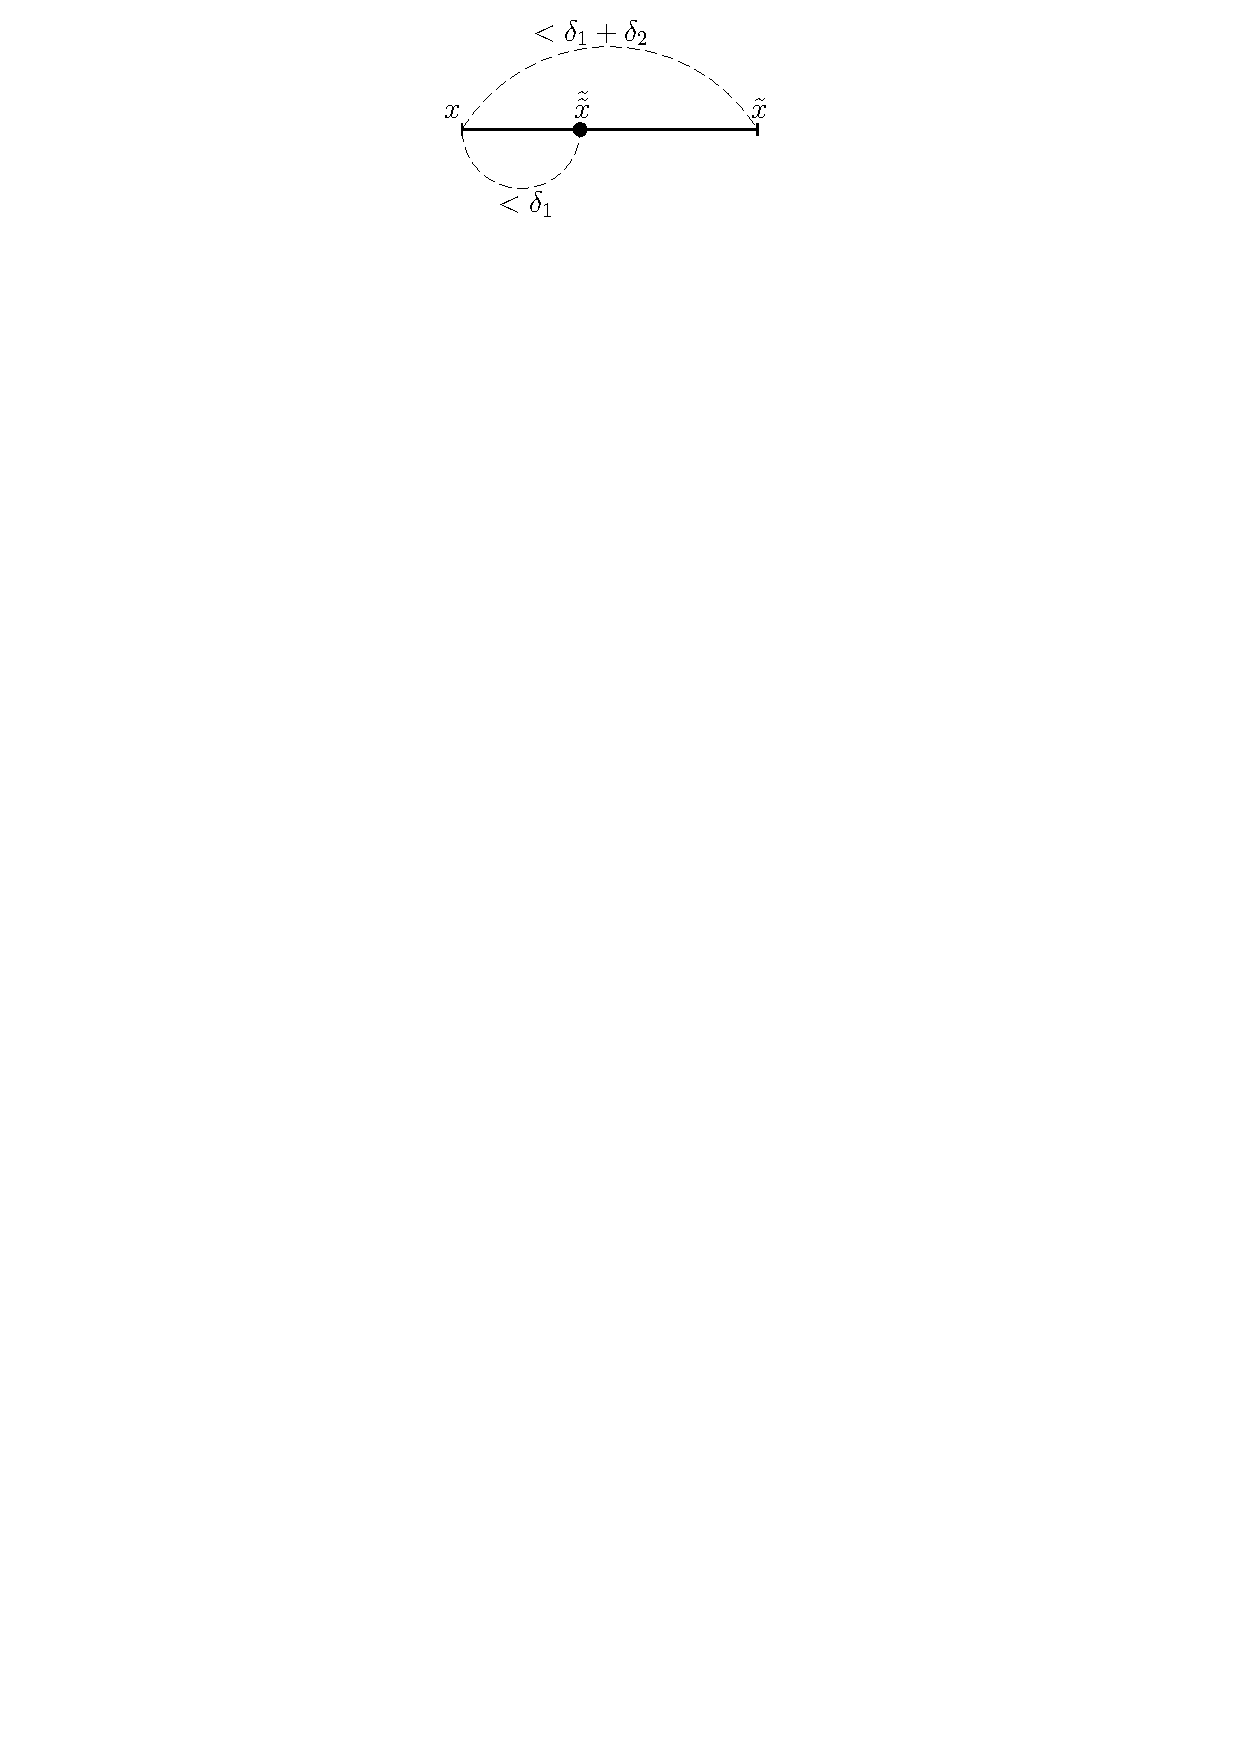
\includegraphics[height=2.7cm]{img/final/galat/Rasr/delt.pdf}\caption{Только для промежутков!}
\end{figure}

Тогда $|f(x)-f(\tilde x)|\hm=|f(x)-f(\tilde{\tilde x})+f(\tilde{\tilde x})-f(\tilde x)|\leq
|f(x)-f(\tilde{\tilde x})|+|f(\tilde{\tilde x})-f(\tilde x)|
\leq \omega_f(\delta_1)+\omega_f(\delta_2)\hm{\hm{\imp}} \omega_f(\delta_1)+\omega_f(\delta_2)$ "--- какая-то верхняя грань.

Значит, $\underbrace{\sup\limits_{\begin{smallmatrix}
    x,\tilde x\in A\\ |x-\tilde x|\hm<\delta_1+\delta_2
    \end{smallmatrix}}|f(x)-f(\tilde x)|}_{\hm=\omega_f(\delta_1+\delta_2)}
    \leq \omega_f(\delta_1)+\omega_f(\delta_2)$.
\end{Proof}

Действительно, $\tilde{\tilde x}$ можно найти, но лежит ли она в~множестве $A$? Что надо потребовать, чтобы такая точка $\tilde{\tilde x}$ в~множестве $A$ нашлась:
пусть \textbf{$A$ "--- промежуток}, "--- без этого утверждение становится неверным.

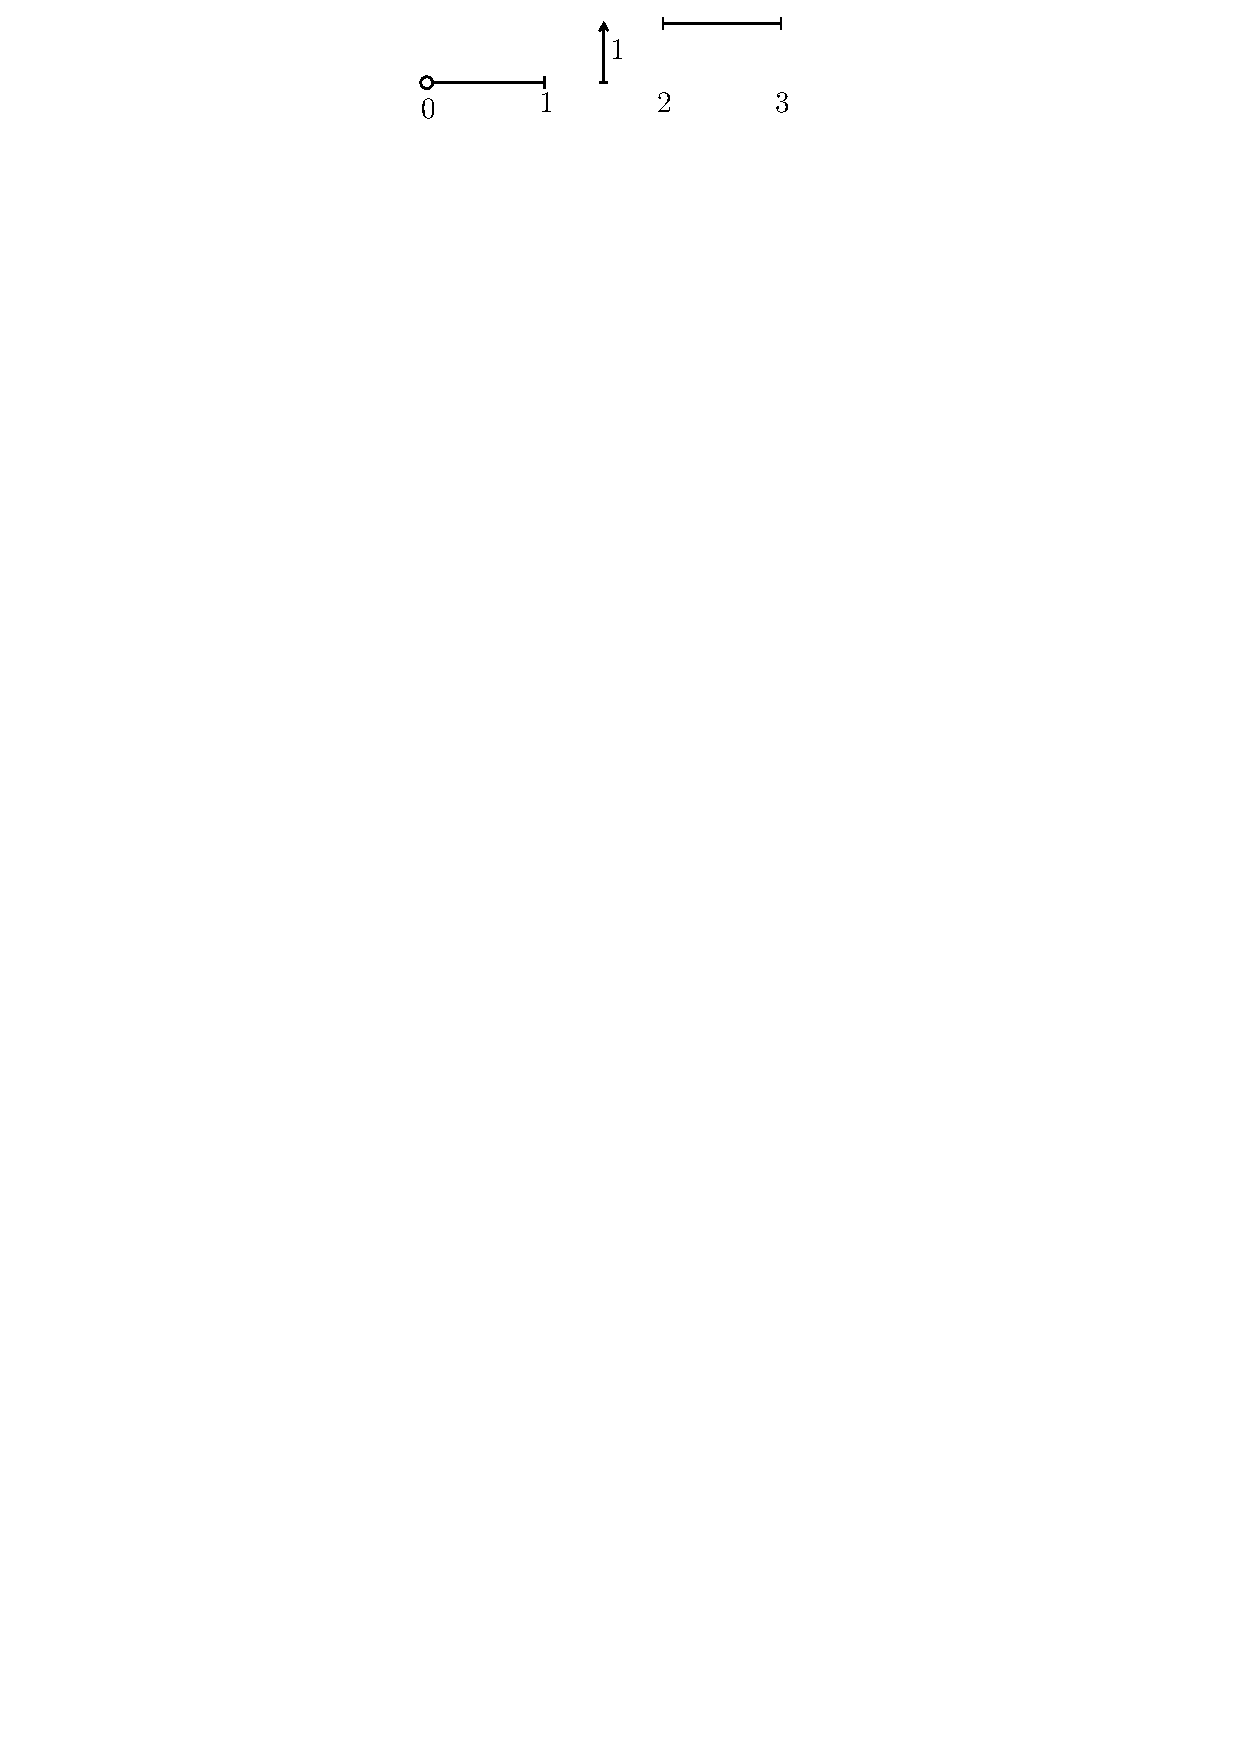
\includegraphics[height=1cm]{img/final/galat/Rasr/nepromeg.pdf}
$\begin{matrix}
\omega_f(1)\hm=0\\
\omega_f(2)\hm=1
\end{matrix}$, важно, чтобы множество было не особо дырчатым;


\item $f$ "--- равномерно непрерывна на~множестве $A \hm{\iff} \lim\limits_{\delta\to0+}\omega_f(\delta)\hm=0$. Часто предел справа обозначают просто $f(x+0)$, поэтому так же часто пишут $\omega_f(\delta+0)$.
\end{enumerate}

\begin{Proof}
Давайте быстренько докажем: Начнём с~$\hm{\imp}$: зафиксируем произвольное $\e\hm>0$. Для $\e_1\hm=\dfrac{\e}2$ из~определения равномерной непрерывности найдём $\delta_0\hm>0\colon
\forall\  x,\tilde x\in A\colon |x-\tilde x|\hm<\delta_0\pau |f(x)-f(\tilde x)|\hm<\e_1$. Тогда, что мы можем сказать про $\omega_f(\delta_0)$? $\omega_f(\delta_0)\leq\e_1\hm<\e\hm{\imp}
\forall\ \delta\in(0,\delta_0)\pau 0\leq \omega_f(\delta)\leq \omega_f(\delta_0)\hm<\e$ в~силу уже установленной монотонности. Мораль: мы доказали, что $\lim\limits_{\delta\to0+}\omega_f(\delta)\hm=0$.

Теперь $\Leftarrow$: знаем, что $\omega_f(\delta+0)\hm=0$. Зафиксируем $\e\hm>0$. из~определения предела найдём такое $\delta_0\hm>0$, что
$\forall\  \delta\in(0,\delta_0)\pau |\omega_f(\delta)-0|\hm<\e$. $\omega_f(\delta)\hm<\e$, ну зачем модуль писать, если $(0,+\infty)\to[0,+\infty]$. Положим
$\delta\hm=\dfrac{\delta_0}2$, главное, чтобы $\delta\in(0,\delta_0)$. Тогда $\forall\  x,\tilde x\in A
\colon |x-\tilde x|\hm<\delta\pau |f(x)-f(\tilde x)|\leq \omega_f(\delta)\hm<\e$. Мы и установили: $f$ "--- равномерно непрерывна на~множестве $A$.
\end{Proof}

Какой вывод: может $\omega_f(\delta)\hm=\delta^2$? Не может\footnote{
$\omega_f\left(\frac12+\frac12\right)\hm=1\hm>\frac12\hm=\frac14+\frac14\hm=\omega_f\left(\frac12\right)+\omega_f\left(\frac12\right)$, противоречит свойству \ref{wf2}.}
. а~$\omega_f\equiv0\hm{\iff} f\hm=\const$.

\begin{Sl}
Если функция просто непрерывна на~отрезке $[a,b]$, то $\omega_f(+0)\hm=0$.
\end{Sl}

$\omega_f(\delta)$ "--- зависимость худшего расклада от задаваемого изменения $\delta$.

\textit{Семейный студент: если концентрируется на~семье "--- вырастают хвосты,
концентрируется на~учёбе "--- вырастают рога, концентрируется и на~том и на~другом "--- быстро отбрасывает копыта.}

Давайте вспомним: промежуток "--- подмножество числовой прямой, который вместе с~$\forall\  a,b$ содержит все промежуточные.

\begin{Ut}
Образ промежутка при непрерывном отображении "--- промежуток. Если $I$ "--- промежуток, $f\in C(I)$, то $f(I)$ "--- промежуток (следует из~теоремы \ref{bk} Больцано"--~Коши о промежуточных значениях)
\end{Ut}

\begin{Ut}
Пусть $I$ "--- промежуток, $f$ монотонна (строго или нестрого) на~$I$. Следующие утверждения эквивалентны:

\begin{enumerate}
    \item $f$ непрерывна на~$I$.

    \item Образ $f(I)$ "--- промежуток.
\end{enumerate}
\end{Ut}

\begin{Proof}
($1\hm{\imp}2$): для любой непрерывной функции, не обязательно монотонной, верно (предыдущее утверждение).

($2\hm{\imp}1$): Рассмотрим случай $f\nv$. Пусть $x_0\in I(x_0$ не является правым концом $I$). Возьмём $x_1\in I\colon
x_1\hm>x_0$. Посмотрим, какие значения принимает $\big[f(x_0),f(x_1)\big]\supset f\big((x_0,x_1]\big)\supset\big(f(x_0),f(x_1)\big]$

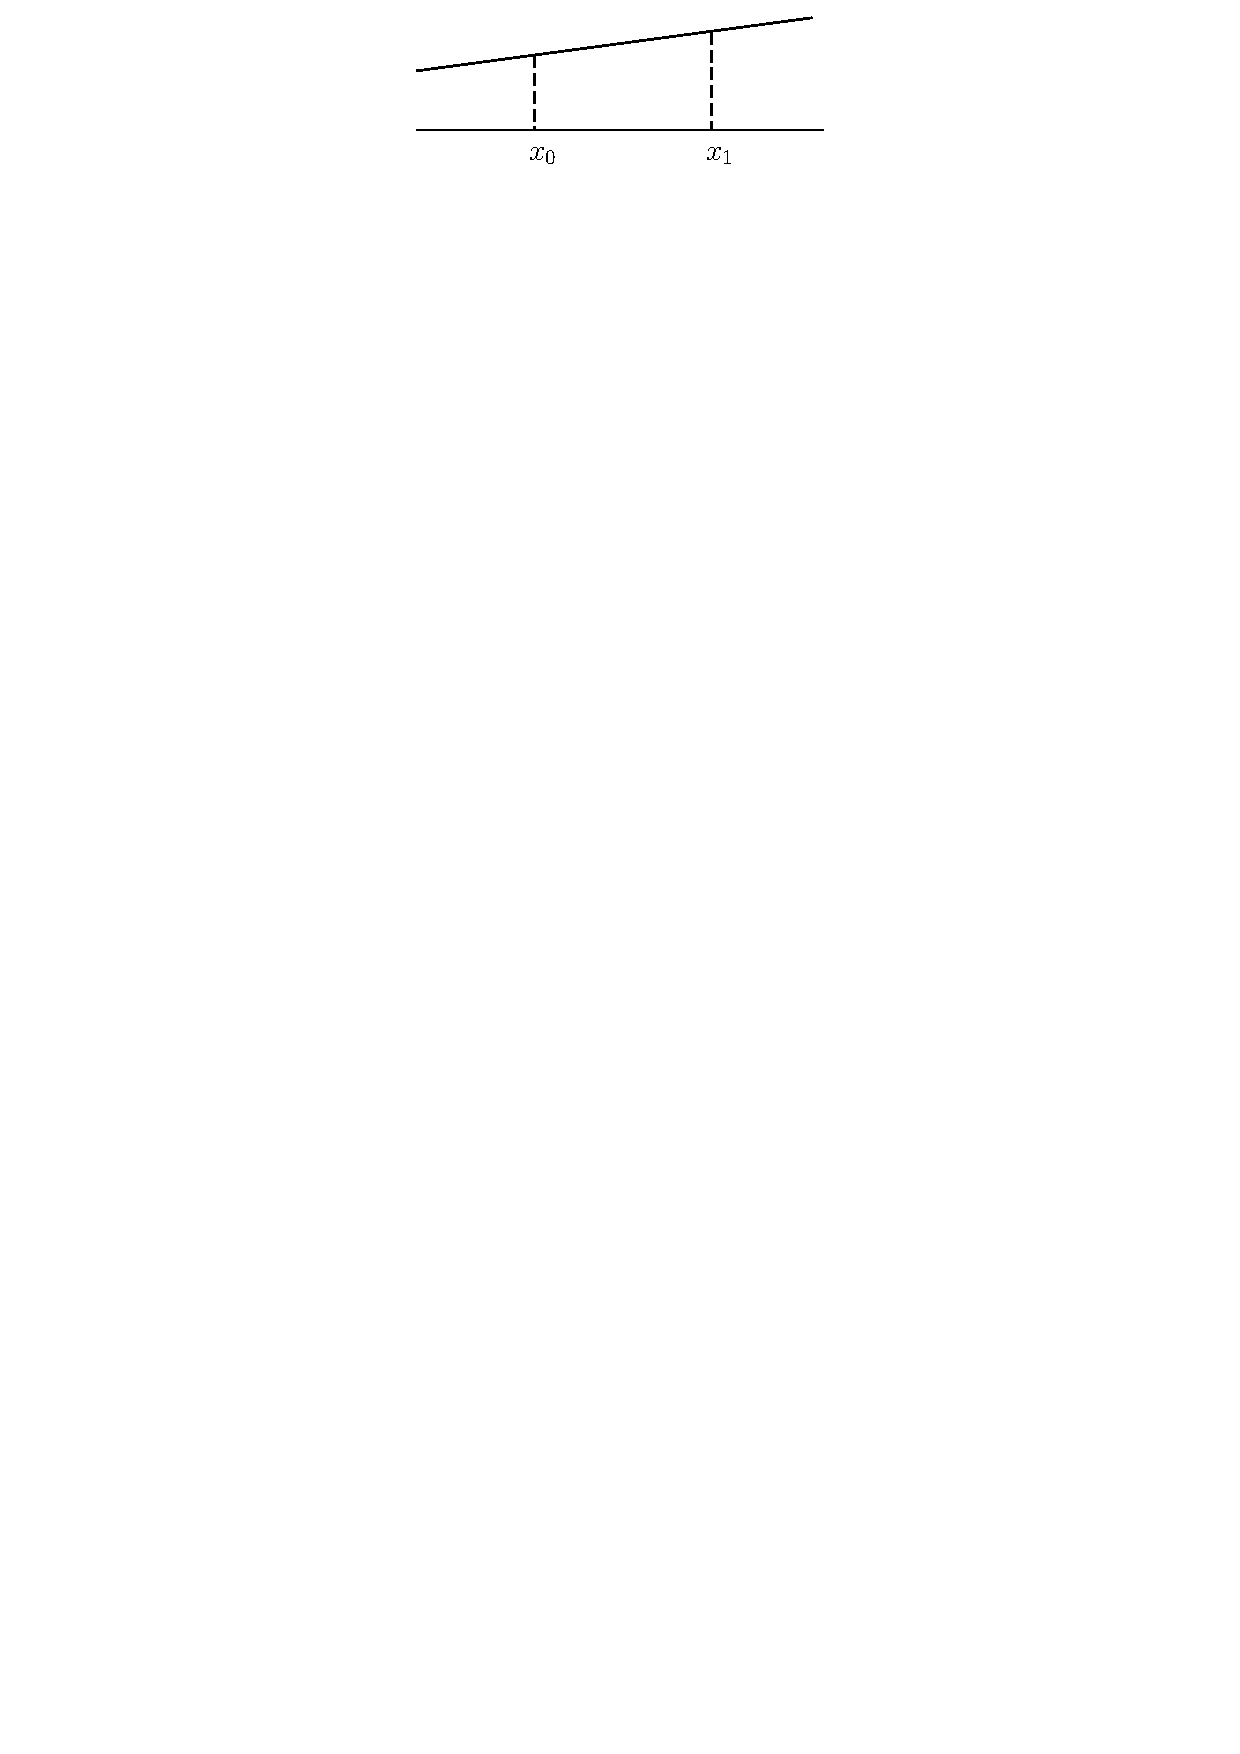
\includegraphics[height=2cm]{img/final/galat/Rasr/bk.pdf} "--- принимает все свои промежуточные значения (теорема \ref{bk}).

$\lim\limits_{x\to x_0+}f(x)\hm=\inf\limits_{x\in(x_0,x_1]}f(x)\hm=f(x_0)\hm{\imp} f(x_0)\hm=
\lim\limits_{x\to x_0+0}f(x)$. Аналогично для другого одностороннего предела.
\end{Proof}

\begin{Ut}
Пусть $I$ "--- промежуток, $f\in C(I)$, $f$ обратима на~$I$. Тогда $f$ "--- строго монотонна на~$I$, $f(I)\hm=J$ "--- промежуток, $f^{-1}\colon J\to I$. С~обозначениями разобрались
\end{Ut}

\begin{Proof}
Пусть $x_1,x_2$ "--- произвольные точки $I\colon x_1\hm<x_2$. Предположим $f(x_1)\hm<f(x_2)$, (случай  $f(x_1)\hm>f(x_2)$  аналогично) $f(x_1)\hm=f(x_2)$ невозможно, ибо не будет обратима.
\end{Proof}

\section{Непрерывность и монотонность. Новые функции}

\subsection{Как связаны свойства непрерывности и монотонности}

\begin{Ut}\label{ints}
Пусть $f$ монотонна на~интервальчике $(a,b)$, в~этом же интервальчике есть такие иксы: $x_n\underset{n\to\infty}\nearrow b$ (возрастает к~значению $b$), тогда
$\lim\limits_{x\to b-0}f(x)$ и $\lim\limits_{n\to \infty}f(x_n)$ на~расширенной числовой прямой существуют и равны. Для монотонной функции достаточно только одной последовательности.
\end{Ut}

\begin{Proof}
$\lim\limits_{x\to b-0}f(x)$ (конечный или бесконечный) существует в~силу монотонности $f$. Остаётся использовать определение \ref{ge} предела по~Гейне.
\end{Proof}

\begin{Ut}
{Пусть} $f$ "--- монотонна на~$(a,b)$ и $x_n\searrow a$. Тогда $\lim\limits_{x\to a+0}f(x)$ и $\lim\limits_{n\to \infty}f(x_n)$ существуют на~$\ol\R$ и равны.

\end{Ut}

\begin{Th}
Пусть функция $f$ непрерывна на~$[a,b]$ и инъективна на~$[a,b]$ Тогда $f$ "--- строго монотонна на~$[a,b]$.
\end{Th}

\begin{Proof}
Так как $f(x)$ "--- инъективно, $f(a)\neq f(b)$. Рассмотрим $f(a)\hm>f(b)$ (второй случай аналогично). Покажем сначала, что
$\forall\  c\in(a,b)\pau f(b)\hm<f(c)\hm<f(a)$.

Ну это очень несложно.

\begin{figure}[htbp]\centering
    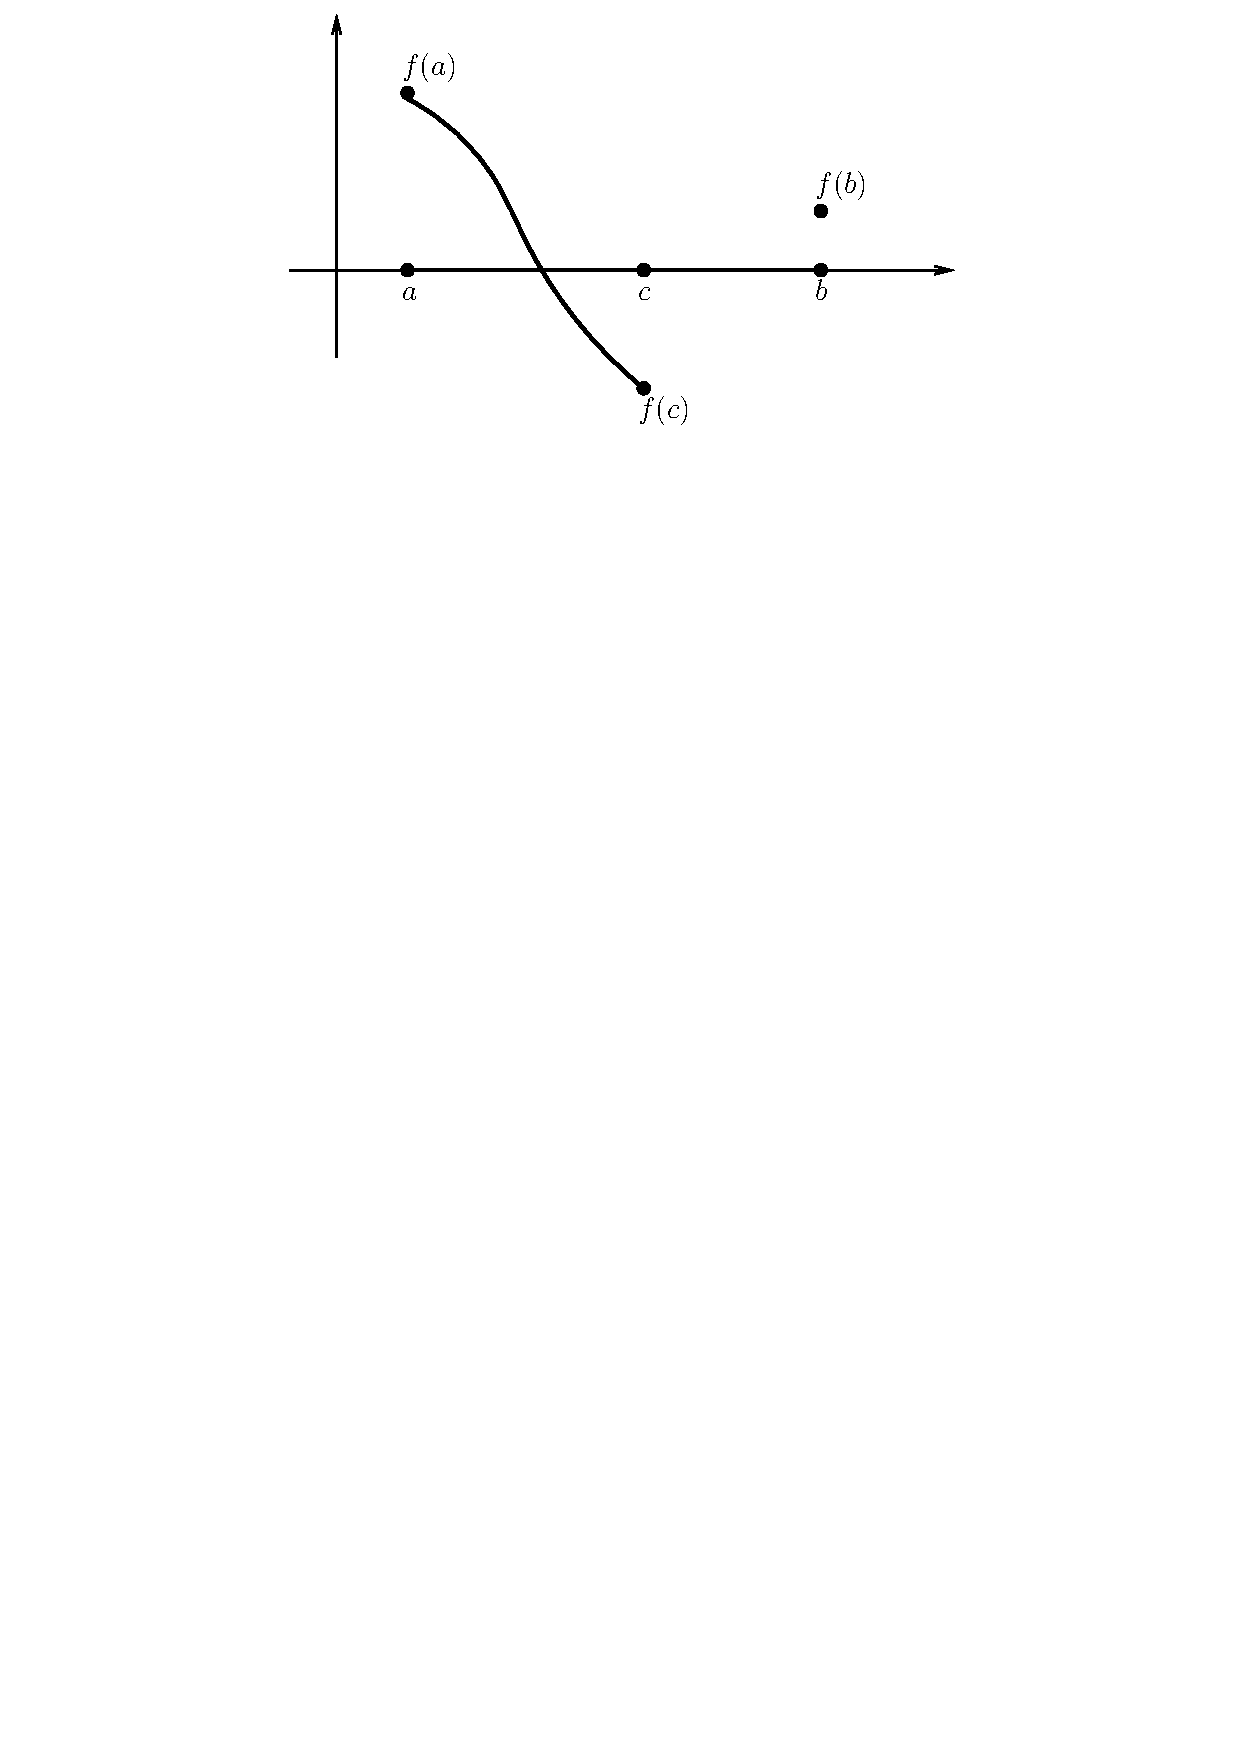
\includegraphics[height=4cm]{img/final/galat/Rasr/abc.pdf}\caption{Непрерывна и инъективна, значит, строго монотонна.}
\end{figure}

Если $f(c)\leq f(b)$, то на~$[a,c]\pau \exists\  x_0\colon
f(x_0)\hm=f(b)$ (по теореме \ref{bk} о промежуточных значениях).

Аналогично, если $f(c)\geq f(a)$ "--- вылезет в~другую сторону, то $\exists\  x_0\in [c,b]\colon f(x_0)\hm=f(a)$


Ответ на~исключительного ума вопрос из~аудитории: \textit{
Наверно, термин «хакер» знаете, ваше поколение, наверное, знает ещё, кто такой «ламер». на~всякий случай «ламер» "--- это такой «антихакер». Абсолютно без всяких намёков на~связь этой истории с~услышанным вопросом: приходит как-то раз ламер к~хакеру
с распечаткой кода и спрашивает «Где? Где же тут ошибка?», ответ: «Наверно в~ДНК». Абсолютно не знаю, почему вспомнил эту историю.}

В любом случае инъективность оказалась нарушена. Значит, $f(b)\hm<f(c)\hm<f(a)$. Но это мы ещё не доказали строгое убывание. Пусть теперь $x_1,x_2$ "--- произвольные точки $[a,b]$, причём $x_1$ поменьше, чем $x_2$ ($x_1\hm<x_2$). Покажем, что $f(x_1)\hm>f(x_2)$, тем самым мы покажем, что $f$ строго убывает. $f(x_2)\hm<f(a)$ по~доказанному. Остаётся применить доказанное утверждение к~отрезку $[a,x_2]$: на~$[a,x_2]\ f$ тоже непрерывна и инъективна $\hm{\imp} f(x_2)\hm<f(x_1)\leq f(a)$, это и доказывали.

\end{Proof}

\begin{Sl}
Пусть $I$ "--- невырожденный промежуток, $f$ "--- непрерывна на~$I$ и инъективна на~$I$. Тогда $f$ строго монотонна на~$I$.
\end{Sl}

\begin{Proof}
Пусть $a,b$ "--- произвольные точки $I\colon a\hm<b$. Рассмотрим $f(a)\hm>f(b)$, покажем, что $f\searrow$ на~$I$. Пусть $x_1,x_2\in I\colon x_1\hm<x_2$. Через $A$ обозначим $\min\{x_1,a\}$, через $B$ обозначим $\max\{x_2,b\}$.
Отрезок $[A,B]\subset I$, ведь $\{x_1,x_2,a,b\}\subset I$. Тогда $f\in C\big([A,B]\big)$ "--- на~большем промежутке непрерывна, на~части этого промежутка тем более. $f$ инъективна на~$[A,B]\hm{\imp} f$ строго монотонна на~$[A,B]$. Рассматривая пару точек $a,b$ делаем вывод, что $f\searrow$, значит $f(x_1)\hm>f(x_2)$.
\end{Proof}

Пусть $I$ "--- невырожденный промежуток. $f\in C(I)$. Множество значений $f(I)\hm=J$ "--- промежуток.

Вывод из~леммы: если функция обратима, то есть отношение между элементами $J$ и $I$ является отображением, то $f$ строго монотонна на~$I$.

\begin{Sl}\label{obnep}
Предположим теперь, что $f\in C(I)$ и строго монотонна на~$I$. Тогда $f$ является биекцией $I$ на~$J\hm{\iff} \exists\  $ обратное
отображение $J$ на~$I$, обозначим $f^{-1}$: $f^{-1}$ строго монотонна на~$J$ с~тем же характером монотонности, что и у функции $f$,
множество значений которой всё $I$ "--- промежуток $\hm{\imp} f^{-1}$ непрерывна на~$J$.
\end{Sl}

Мораль: мы закончили небольшой кусочек про обращение непрерывной функции. После этого хочется перейти к~нормальному анализу, но вот беда: не понимаем, что значит объект, с~которым мы работаем.
Что такое $e^{\sqrt2}$, например?
\subsection{Введение функций}

\textit{Есть как минимум две нестандартные логики: женская и логика программистов "--- для внешних людей совершенно необъяснимые. Жена программиста говорит мужу: «купи яиц десяток, батонов купи, колбасы». Программист приходит в~магазин: «яйца есть? Нет? Ну тогда дайте десяток батонов колбасы!»}

Что такое для $n\in\N\pau x^n$? $x^n\hm=\underbrace{x\cdot x\cdot\ldots\cdot x}_n$ "--- произведение $n$ иксов. Можем рассмотреть $f(x)\hm=x^n$. Во-первых $x^n\in C(\R)$. $x^n$ при нечётных $n\nearrow$ на~$\R$, при чётных $n\begin{matrix}
\nearrow\text{на }\R^+\\ \searrow\text{на }\R^-
\end{matrix}$.

Определим $x^{\frac1n}$ как функцию, обратную к~$x^n$ ($\sqrt[n]x$). \begin{tabular}{l}Для чётных $n\pau \sqrt[n]x\colon \R^+\to\R^+$\\Для нечётных $n\pau \sqrt[n]x\colon \R\to\R$\end{tabular}. $\sqrt[n]x$ "--- $\nearrow$ непрерывная
функция (ведь обратная к~строго возрастающей непрерывной).
Для $n\in\{-1,-2,\ldots\}\pau x^n\hm=\dfrac1{x^{-n}}$ "--- определена и непрерывна на~$\R\dd\{0\}\hm{\imp}$
\begin{tabular}{l}
на $(0,+\infty)$ строго убывает;\\
на $(-\infty,0)$ растёт при чётных $n$ и убывает при нечётных $n$.
\end{tabular}

Для $a\hm>0,\ r\in\Q\pau \left(r\hm=\dfrac mn,\text{ где } m\in\Z,\ n\in\N\right)$ определим $a^r\hm=\sqrt[n]{a^m}$ "--- ну примерно так или наоборот.
Для всех чисел $x\neq0$ положим $x^0\hm=1$.

Это определение корректно: не зависит от представления $r$ в~виде дроби $\Big(\dfrac mn$ или $\dfrac{2m}{2n}\ldots\Big)$.
 $a^{r_1}a^{r_2}\hm=a^{r_1+r_2}$ "--- показательная функция переводит мультипликативную шкалу в~аддитивную. $(a^{r_1})^{r_2}\hm=a^{r_1r_2},\pau a^rb^r\hm=(ab)^r$.

 Что более важно: функция $f(x)\hm=x^r\ (r\in\Q)$ определена на~$(0,+\infty)$, непрерывна на~этом интервале, $\nearrow$ при $r\hm>0$, $\searrow$ при $r\hm<0$.

 Зафиксируем $a\hm>0$. Определено $a^r\ (\Q\to\R$ "--- не все, но какие-нибудь получим). При $a\hm=1\pau a^r\equiv1$, $a\hm>1\pau a^r\nearrow$, $a\hm<1\pau a^r\searrow$

 \begin{Proof}
Пусть $a$ лежит между нулём и единицей: $a\in(0,1),\pau
r_1,r_2\in\Q\colon r_1\hm<r_2$. Покажем, что $a^{r_1}\hm>a^{r_2}$. Что такое $a^{r_2}-a^{r_1}$? Это ровно тоже самое, что $a^{r_1}(a^{\overbrace{r_2-r_1}^{\hm>0}}-1)\hm<a^{r_1}(1^{r_1-r_2}-1)\hm=0$ (использовали монотонность $x^r$).
 \end{Proof}

 \begin{Th}
$\forall\  a\hm>0\pau \underset{\begin{matrix}\begin{sideways}\hm=\end{sideways}\\a^{\frac1n}\end{matrix}}{\sqrt[n]a}\te 1$
 \end{Th}

\begin{Proof}
    При $a\hm=1$ утверждение тривиально. Докажем при $a\hm>1$: $a^{\frac1n}\underset{n\to\infty}{\searrow}$ и $a^{\frac1n}\hm=a^{\frac1n}\cdot1^{\frac1n}\hm>1^{\frac1n}\hm=1$.
    с~другой стороны: любое число, большее единицы, не является нижней гранью множества значений последовательности $\sqrt[n]a$: пусть $\alpha\hm>0$,
     покажем, что неравенство $a^{\frac1n}\geq1+\alpha$ неверно для $n\hm=\left[\frac{a}{\alpha}\right]+1$. $a\geq(1+\alpha)^n\hm>1+\alpha n\hm>\alpha n$.
     Мораль: $1$ является точной нижней гранью множества значений последовательности,
    по~теореме \ref{The18} о монотонно убывающей последовательности $\lim\limits_{n\to\infty}a^{\frac1n}\hm=1$.

    Для $a\in(0,1)\pau \sqrt[n]a\hm=\dfrac{1}{\sqrt[n]{\vphantom{\frac1a}\left(\frac1a\right)}}\db{\text{ по}}{\hm>1}{}$ доказанному знаменатель стремится к~единице.
\end{Proof}


\section{Иррациональные показатели}

Напомню: возведение в~натуральную степень и в~целую вытекает из~простой функции $x$. далее $x^n\rightsquigarrow\sqrt[n]x$ для $n\in\N$.
Потом возникает понятие возведения в~рациональную степень: $x^{\frac mn}\hm=\sqrt[n]{x^m}\ (x\hm>0$, чтобы не было проблем). Ещё один простенький результат:
$\forall\  a\hm>0\pau \sqrt[n]{a}\te1$. Возникла $a^x$ пока только для рациональных чисел, $a^x\colon \Q\to(0,+\infty)$.

\begin{Ut}\label{vdeg}
    $\forall\  a\hm>0,\ \forall\  x_0\in\R$ односторонние пределы $\yo{\Q\ni x}{x_0-0}a^x$ и $\yo{\Q\ni x}{x_0+0}a^x$ существуют и равны (и для рациональных $x_0$ они равны $a^{x_0}$).
\end{Ut}

\begin{Proof}
    Для $a\hm=1$ здесь доказывать нечего. Рассмотрим случай $a\hm>1$ (другой случай $\frac1a\hm>1$), эта штука является строго возрастающей, соответственно:

    \begin{tabular}{ll}
    $\forall\  x\in\Q\colon$&$x\hm<x_0$\\
    $\forall\  \tilde x\in\Q\colon$&$\tilde x\hm>x_0$
    \end{tabular} какие выводы можно сделать? Ну, во-первых: $a^x\hm<a^{\tilde x}$, ну а~во-вторых: если точка $x_0\in\Q\colon a^x\hm<a^{x_0}\hm<a^{\tilde x}$, то значит
    $s\hm=\lims{\sup a^x}{x\in\Q}{x\hm<x_0}\leq a^{\tilde x}$ "--- верхняя грань, она не является точной верхней гранью. Значит
    $i\hm=\lims{\inf a^{\tilde x}}{\tilde x\in\Q}{\tilde x\hm>x_0}\geq s$.

    с~другой стороны: пусть $\pos x$ и $\pos{\tilde x}$ "--- последовательности рациональных чисел такие, что

    \begin{tabular}{ll}
        во-первых:&$\forall\  n\in\N\pau x_n\hm<x_0\hm<{\tilde x}_n$\\
        а~во-вторых:&$({\tilde x}_n-x_n)\hm=\frac1n$
    \end{tabular}

    \begin{figure}[htbp]\centering
    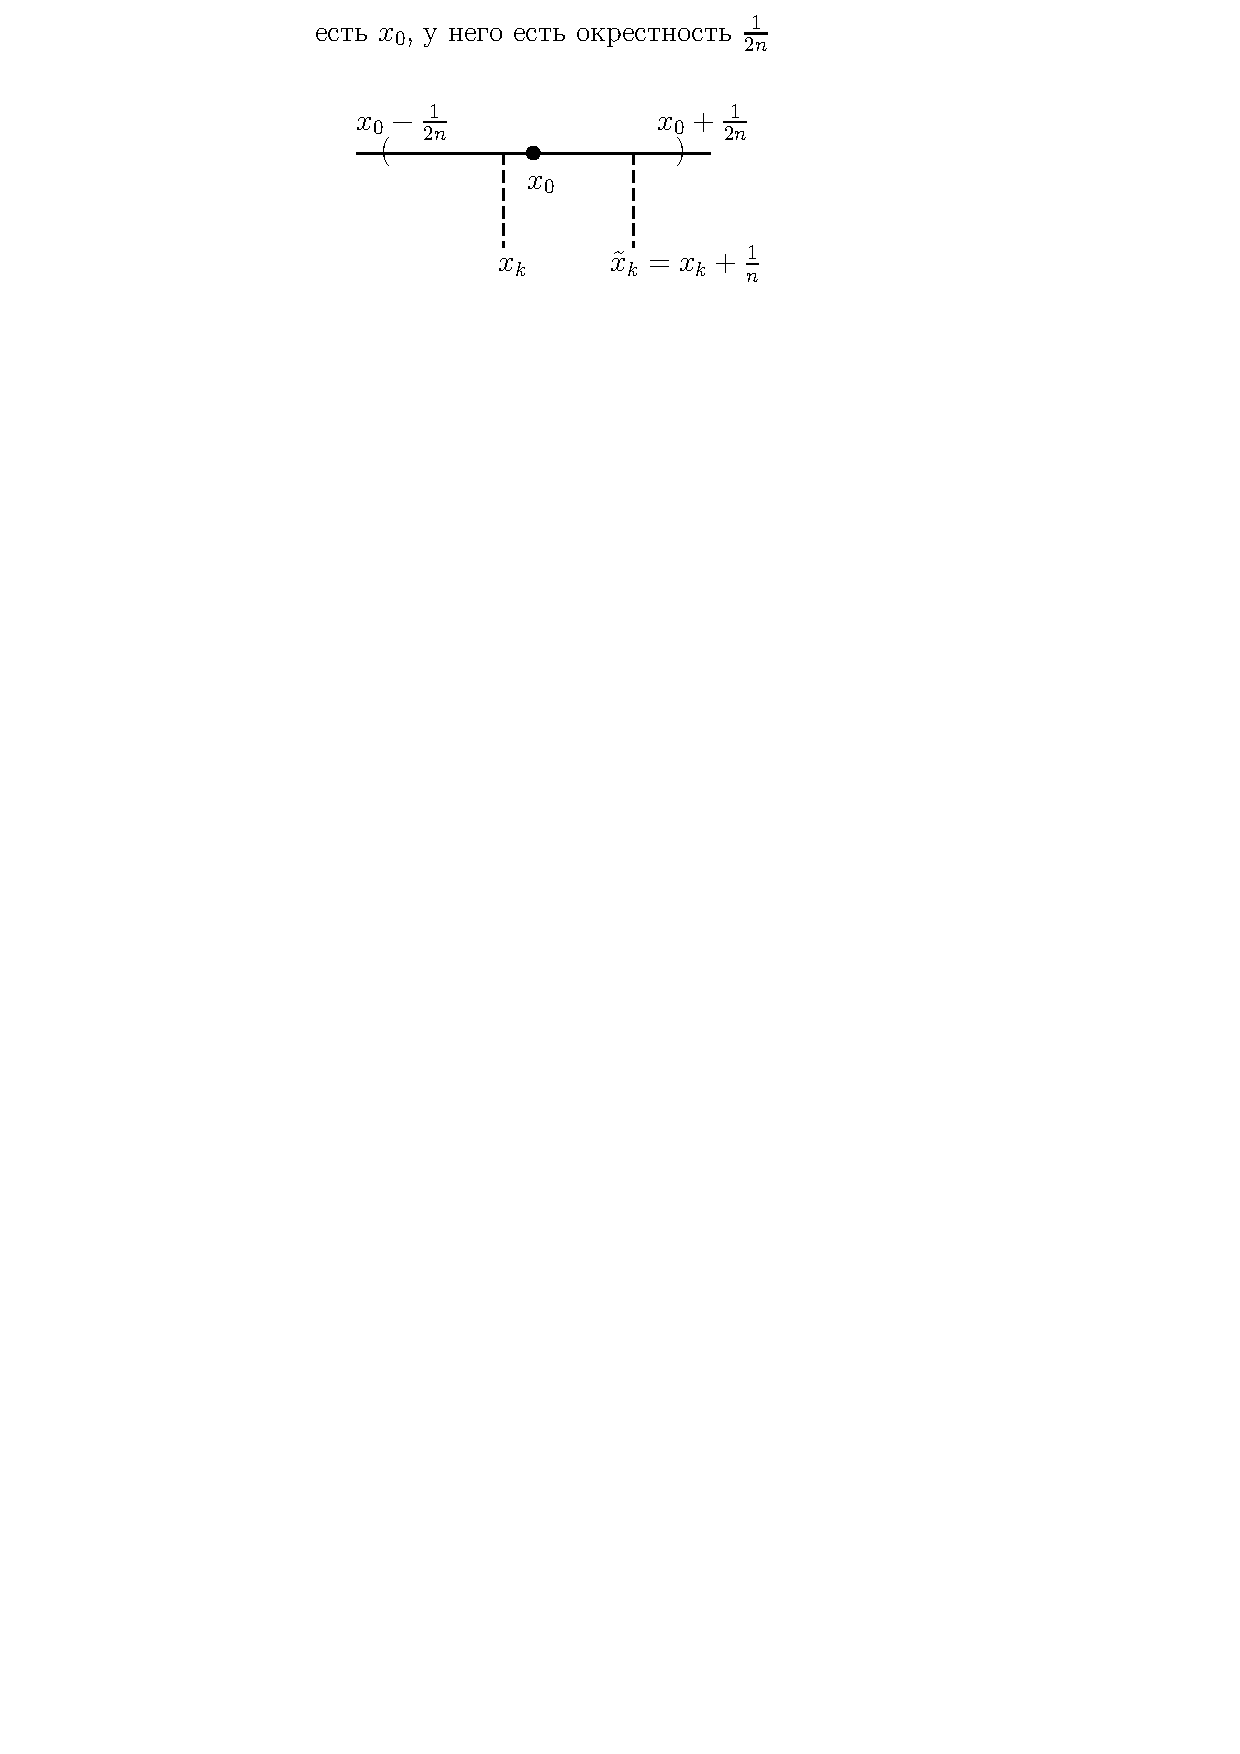
\includegraphics[height=3.5cm]{img/final/galat/vvedf/pokaz.pdf}\caption{Рациональные точки}
\end{figure}

А насколько могут отличаться $i$ и $s$? $(i-s)\leq \underbrace{a^{{\tilde x}_n}}_{\geq i}-\underbrace{a^{x_n}}_{\leq s}$.

$0\leq(i-s)\leq a^{{\tilde x}_n}-a^{x_n}\hm=a^{x_n}\left(a^{\frac1n}-1\right)\leq$ на~всякий случай перепишу ещё и вот так: $\leq
a^y\left(a^{\frac1n}-1\right)$, где $y$ "--- произвольное фиксированное рациональное число: $y\hm>x_0$ (Ну не хочу я~так зависимость от $n$, ну не хочу).
Тогда $a^y\left(a^{\frac1n}-1\right)\te0$. Делаем вывод: $i$ и $s$ "--- это одно и то же. Мы уже всё доказали. Перепишу ещё раз неравенство
$a^x\hm<a^{x_0}\hm<a^{\tilde x}$. Что такое $\yo{\Q\ni x}{x_0-0}{a^x}$? Это величина у нас равна $s$ (ведь $\nearrow$ функция).
$\yo{\Q\ni x}{x_0+0}a^x\hm=i$. Ну, значит, пределы действительно одинаковы.

Ещё раз внимательно посмотрим на~неравенство $s\leq a^{x_0}\leq i$, а~$i\hm=s\hm{\imp} a^{x_0}$ принимает ровно то же значение.
\end{Proof}

Это позволяет определить возведение в~произвольную степень.

\begin{Def}
    $\forall\  a\hm>0$ и $x_0\in\R$ положим $a^{x_0}\hm=\yo{\Q\ni x}{x_0\pm0}a^x$
\end{Def}

Наша лемма (утверждение \ref{vdeg}) утверждает, что наше определение корректно. а~для $x\in\Q$  у нас уже два определения. Но значение выдаётся одно и то же.

Какие свойства есть у этой функции:

\begin{tabular}{lll}
    \multicolumn{3}{c}{$a^x$ называется показательной функцией}\\
    $\bullet$&\multicolumn{2}{l}{$a^x$ определена на~$\R$}\\
    $\bullet$&\multicolumn{2}{l}{Множество значений: $(0,+\infty)$ при $a\neq 1$}\\
    $\bullet$&При $a\hm>1$&$ a^x\nearrow$ на~$\R$\\
    $\bullet$&При $a\in(0,1)$&$a^x\searrow$ на~$\R$\\
    $\bullet$&$\forall\  a\in(0,+\infty)$&$a^x\in C(\R)$
\end{tabular}

\begin{Proof} (Монотонность) $a\hm>1$ (второй случай рассматривается аналогично). Пусть $x_1\hm<x_2$. Найдём $\tilde x_1,\tilde x_2\in\Q\colon
x_1\hm<\tilde x_1\hm<\tilde x_2\hm<x_2$. Тогда, что можем сказать про $a^{x_1}$ и $a^{\tilde x_1}$? на~$\Q\pau a^x$ возрастает. Переход к~пределам сохраняет нестрогие неравенства (утверждение \ref{pernes}):
$\dt{a^{x_1}\leq a^{\tilde x_1}\hm<a^{\tilde x_2}\leq a^{x_2}}{|}{\text{рациональные степени}}{\text{можно и $\hm<$}}$

\end{Proof}

Теперь неплохо бы установить непрерывность.

\begin{Proof}
    Пусть $x_0$ "--- произвольная точка $\R$. $\pos x$ "--- последовательность рациональных чисел, ну неважно, возрастающая к~$x_0$. Тогда
    $\lefteqn{\dt{\phantom{\yo{x}{x_0-0}a^x\hm=\yo{n}{\infty}a^{x_n}}}{\qquad|}{\text{используем монотонность}}{\text{(утверждение \ref{ints})}}}
    \yo{x}{x_0-0}a^x\ \ \hm=\ub{\yo{n}{\infty}a^{x_n}\ \hm=\yo{\Q\ni x}{x_0-0}}{|}{\text{определение \ref{ge} Гейне}}a^x\hm=a^{x_0}$.

   Абсолютно аналогично: $\yo{x}{x_0+0}a^x\hm=a^{x_0}$. Значит $\exists\  \yo x{x_0}a^x\hm=a^{x_0}$, а~это непрерывность в~точке $x_0$.
   Вывод: наша функция непрерывна на~всей числовой прямой.
   \end{Proof}

   \begin{Ut}
   Если $a\hm>1$, то $\yo x{+\infty}a^x\hm=+\infty$.
   \end{Ut}

   \begin{Proof}
    Куча способов обоснования: $a\hm=1+\alpha\hm>0$. $\yo{x}{\infty}a^x\hm=\yo{n}{\infty}a^n\hm=\yo{n}{\infty}(1+\alpha)^n\geq\yo{n}{\infty}(1+\alpha n)\hm=+\infty$.
   \end{Proof}

   Ну а~чему равен предел $\yo{x}{-\infty}a^x$? Это ровно то же самое, что и $\yo{\tilde x}{+\infty}\dfrac1{a^{\tilde x}}\hm=0$.

   Вывод: у нас есть монотонная непрерывная функция, которая подходит с~одной стороны к~$0$, с~другой к~$+\infty$.
   Принимает все промежуточные значения $\R^+$ (теорема \ref{bk} Больцано"--~Коши).

\[
\left.
\begin{array}{ccc}
    a^xa^y & \hm= & a^{x+y} \\
   (a^x)^y & \hm= & a^{xy} \\
    a^xb^x & \hm= & (ab)^x \\
\end{array}
\right\} \text{ "--- мы пока эти свойства устанавливали только для $\Q$.}
\]


   \begin{Proof}
    Выберем какое-нибудь. Пусть $\pos x$ "--- последовательность рациональных чисел $\nearrow x$, $\pos y$ "--- последовательность
    рациональных чисел $\nearrow y$. Тогда $(x_n+y_n)$ "--- последовательность рациональных чисел и она $\nearrow (x+y)$. Что такое
    $a^{x+y}$? а~это вот что: $a^{x+y}\hm=\yo{n}{\infty}a^{(x_n+y_n)}\hm=\yo{n}{\infty}a^{x_n}a^{y_n}\hm=
    \yo{n}{\infty}a^{x_n}\cdot\yo{n}{\infty}a^{y_n}\hm=a^xa^y$.
   \end{Proof}

Пишем свойство для рациональных чисел и переходим к~пределу, где всё стремится, куда надо.

Наконец-то мы чётко определили функцию, которую так активно используем. Получили бесплатно точное определение логарифмической функции. Для
$a\neq1\pau a^x$ непрерывна и строго монотонно отображает $\R$ в~$(0,+\infty)$. Обратная функция существует, является непрерывной, строго монотонной с~тем же характером монотонности (следствие \ref{obnep}).

Логарифмическая функция

   $\log_ax\colon \R^+\to\R$. Обратив свойства, получим: $\log_ax+\log_ay\hm=\log_axy,\ldots$ Всё абсолютно бесплатно.

   $\log_a(xy)\hm=\log_ax+\log_ay$ "--- перевод мультипликативной шкалы в~аддитивную. Так говорить не надо, всё равно никто не поймёт.

На всякий случай: $e^x\hm=\exp(x)$ "--- \textit{е}кспонента, это у нас 33 буквы, а~у них\ldots
$\log_ex\hm=\ln x$

Со скучноватыми вещами на~финишной прямой. Степенная функция: $x^\alpha$ определена и монотонна и непрерывна на~интервальчике $(0,+\infty)$. Принимает значения $(0,+\infty)$.
При $\alpha\hm>0$ допускает непрерывное доопределение нулём в~нуле.
При $\alpha\in\Z$ допускает продолжение на~$(-\infty,0)$. Разберём, почему всё это имеет место для $\alpha\hm>0$ $\left(\vphantom{\frac1{x^\beta}}\right.$для $\alpha\hm<0,\pau \alpha\hm=-\beta\pau x^\alpha\hm=\frac1{x^{-\alpha}}\hm=\left.\frac1{x^\beta}\right)$

\begin{Proof}
    Давайте не спеша, монотонность: пусть $0\hm<x_1\hm<x_2$, что такое $x_2^\alpha-x_1^\alpha$? Это ровно то же самое, что и
$x_2^\alpha-x_1^\alpha\hm=x_1^\alpha\bigg(\underbrace{\left(\tfrac{x_2}{x_1}\right)^\alpha}_{\hm>1}-1\bigg)$.
Если заменить на~меньший $\alpha$, то $\left(\frac{x_2}{x_1}\right)^\alpha$ упадёт.
$x_2^\alpha-x_1^\alpha\hm>x_1^\alpha\bigg(\left(\frac{x_2}{x_1}\right)^0-1\bigg)\hm=0$.
\end{Proof}

\begin{Proof} [Непрерывность в~точке $x_0\hm=1$.] Найдём $n\in\N\colon 0\hm<\alpha\hm<n$. Для $x\hm>1\pau \tud{x^0}{1}\db{\hm<x^\alpha\hm<}{(x\to 1)}{}\tud{x^n}{1}$ "--- про характер монотонности мы знаем$\hm{\imp}\yo{x}{1+0}x^\alpha\hm=1$.

Аналогично: $x\in(0,1)\colon \tud{x^n}{1}\hm<x^\alpha\hm<\tud{x^0}1$ "--- правило сендвича. Вывод: $\yo{x}{1-0}x^\alpha\hm=1\hm{\imp}\yo{x}1x^\alpha\hm=1\hm=1^\alpha$ "--- установили непрерывность в~единице.
\end{Proof}

\begin{Proof}[Непрерывность в~любой другой точке] Пусть
теперь $x_0\in(0,+\infty)$. Что такое $\yo{x}{x_0}(x^\alpha-x_0^\alpha)$? Это ровно то же самое, что и
$\yo x{x_0}x_0^\alpha\bigg(\tud{\left(\frac{x}{x_0}\right)^\alpha}1-1\bigg)\hm=0$
"--- по~только что доказанному. Вывод: $\yo x{x_0}x^\alpha\hm=x_0^\alpha$

\end{Proof}

Найдём $n\colon \frac1n\hm<\alpha\hm<n$. $\ub{\yo{x}{+\infty}x^\alpha\geq
\yo{x}{+\infty}x^{\frac1n}}{|}{\text{(утверждение \ref{pernes})}}\hm=\yo{x}{+\infty}\!\!\!\!\!\!\ub{\sqrt[n]{x}\hm=+\infty}{|}{\text{это уже знаем}}$

$x\in(0,1)\colon 0\leq x^\alpha\leq x^{\frac1n}\pau \yo{x}{0+}x^{\frac1n}\hm=0$

Какие ещё есть хорошие функции? Например, есть у вас тригонометрические функции:
$\sin x,\ \cos x,\ \tg x,\ \ctg x$ (определяемые по~единичной окружности).

Непрерывность синуса: $\forall\  x\hm>0\pau \sin x\hm<x\colon $ 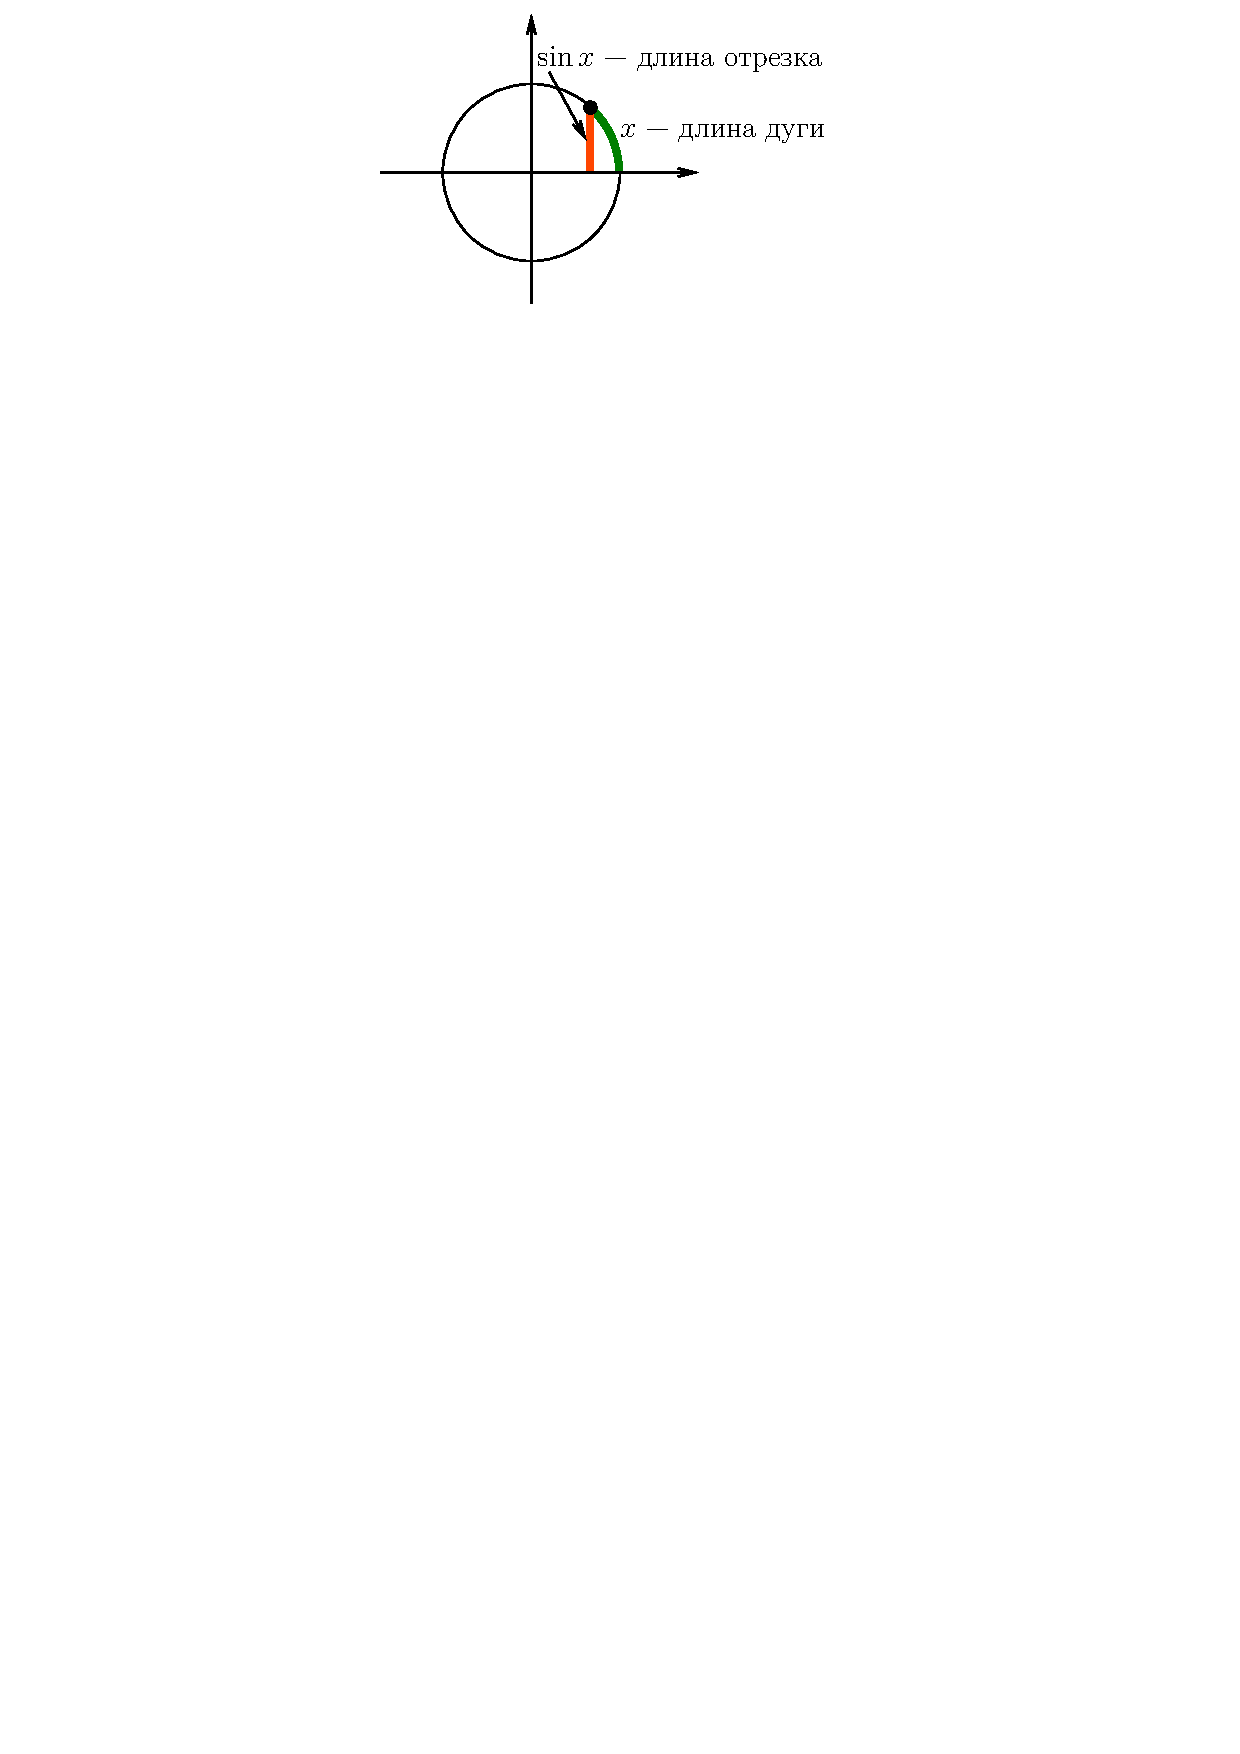
\includegraphics[height=3.5cm]{img/final/galat/vvedf/sinx.pdf}

$\yo{x}{x_0}\sin x-\sin x_0$ "--- где ставить скобки нет никакой разницы. Этот предел равен $\yo{x}{x_0}2\sin\frac{x-x_0}2\cos\frac{x+x_0}2$. $\left|
2\sin\frac{x-x_0}2\cos\frac{x+x_0}2\right|\leq|x-x_0|$\footnote{На всякий случай: это означает, что можно взять $\delta\hm=\e$.}.

$\sin x$ строго возрастающая и непрерывная на~$\left[-\frac{\pi}2,\frac{\pi}2\right]\hm{\imp}
$ существует обратная: непрерывная, возрастающая (следствие \ref{obnep}), называется $\arcsin x$. Для $\cos x$ аналогично.

\begin{Def}
    Простейшими элементарными функциями называют:

    \begin{tabular}{lll}
        $\bullet$&константы\\
        $\bullet$&показательную& $a^x$\\
        $\bullet$&степенную &$x^\alpha$\\
        $\bullet$&логарифмическую\\
        $\bullet$&тригонометрические\\
        $\bullet$&обратные к~тригонометрическим
    \end{tabular}
\end{Def}

\begin{Def}
    Просто элементарные функции "--- функции, полученные из~простейших элементарных конечным числом арифметических операций и композиций.
\end{Def}

$|x|$ элементарная: $|x|\hm=\sqrt{x^2}$.

\subsection{O-символика}

$\ooo{1}{x\to x_0}$

\begin{Def} \label{ot}   $\ouu{1}{x\to x_0}$ "--- ограниченная в~некоторой проколотой окрестности $x_0$.
    Будем говорить, что $f$ ограничена в~точке $x_0$, если $\exists\  \delta\hm>0\colon f$ "--- ограничена в~$B'_\delta(x_0)$

    \end{Def}

    $x^2\hm=\ooo{x^3}{x\to\infty}$

    $x^3\hm=\ooo{x^2}{x\to0}$

    Скучная рутина закончилась.
\section{Замечательные пределы. Производные}
\subsection{Первый замечательный предел.}
$\yo x0\dfrac{\sin x}{x}\hm=1$, в~силу чётности достаточно доказать, что $\lim\limits_{x\to0+}\dfrac{\sin x}{x}\hm=1$. Рассмотрим $x\in\left(0,\frac{\pi}2\right)$.

\pic{galat/23/1zam}{5}{1zam}{Первый замечательный предел.}

Пусть на~единичной окружности (рис. \ref{1zam}) точка $A$ соответствует нулевому углу. Получается дуга $AB$.

$S\triangle_{0AB}\leq S\text{сектор}_{0AB}\leq S\triangle_{0AC}$. Значит, $\dfrac12\cdot1\sin x\leq\dfrac{\pi}{2\pi}\cdot x\leq\dfrac12\cdot\dfrac{\sin x}{\cos x}$.
Домножим на~двойку: $\sin x\leq x\leq \dfrac{\sin x}{\cos x}$, отсюда $\tud{\cos x}1\leq\dfrac{\sin x}{x}\leq\tud11$, ведь $\lim\limits_{x\to0+}{\cos x}\hm=1$.

\subsection{Второй замечательный предел}
\begin{Th}
    $\lim\limits_{x\to\infty}\left(1+\dfrac1x\right)^x\hm=e$
\end{Th}

\begin{Proof}
Для любого $x\hm>0$ найдём такой номер $n$:       $n\leq x\leq n+1$, тогда

$\left(1+\dfrac1{n+1}\right)^n\leq
\left(1+\dfrac1{x}\right)^n\leq
\left(1+\dfrac1{x}\right)^x\leq
\left(1+\dfrac1{x}\right)^{n+1}\leq
\left(1+\dfrac1{n}\right)^{n+1}$

$\left(1+\dfrac1{n+1}\right)^n\hm=\left(1+\dfrac1{n+1}\right)^{n+1}:\left(1+\dfrac1{n+1}\right)$

Зафиксируем произвольное $\e\hm>0$.

Найдём $N_1\in\N\colon
\forall\  n\hm>N_1\pau \left|\left(1+\dfrac1{n}\right)^{n+1}-e\right|\hm<\e$.
Найдём $N_2\in\N\colon
\forall\  n\hm>N_1\pau \left|\left(1+\dfrac1{n+1}\right)^{n}-e\right|\hm<\e$.

Положим $C\hm=\max\{N_1,N_2\}+1$. Тогда $\forall\  x\hm>C$ положим $n\hm=\lfloor x\rfloor$ "--- целая часть снизу ($n\hm>N_1,n\hm>N_2$), и получим
$e-\e\hm<\pzp{n+1}n\leq\pzp xx\leq \pzp n{n+1}\hm<e+\e$, то есть $\left|\pzp xx-e\right|\hm<\e$ и это значит по~определению предела
$\lim\limits_{x\to+\infty}\pzp xx\hm=e$
\end{Proof}

\begin{Th}
    $\lim\limits_{x\to-\infty} \pzp xx \hm=e$
\end{Th}

\begin{Proof}
    Что такое $\lim\limits_{x\to-\infty}\pzp xx\hm=\lim\limits_{y\to+\infty}\left(1-\dfrac1y\right)^{-y}\hm=
    \lim\limits_{y\to+\infty}\left(\dfrac y{y-1}\right)^y\hm=\lim\limits_{y\to+\infty}\pzp{y-1}y\hm=$ $\hm=
    \lim\limits_{y\to+\infty}\tud{\underbrace{\pzp{y-1}{y-1}}}{e}\cdot\tud{\underbrace{\pzp{y-1}{\,\!}}}1\hm=e$
\end{Proof}

Ещё одна теорема:

\begin{The}
    $\yo x0\pz xx\hm=e$
\end{The}

\begin{Proof}
Сперва посмотрим $\yo x{0+}\pz xx\hm=\yo t{+\infty}\pzp tt\hm=e$. Аналогично, $\yo x{0-}\pz xx \hm=\yo t{-\infty}\pzp tt\hm=e$. Итого оба односторонних предела существуют и равны $e$.
\end{Proof}

Какие ещё бесплатные вещи мы можем из~этого получить?

Напомню теорему \ref{tpk} о пределе композиции. Теперь будем её массово использовать.

\begin{Sl}\label{vzpln}
    Что бы сюда написать, ну например: $\yo x0 \dfrac{e^x-1}x\hm=1$ \footnote{На самом деле выйдет $\yo t0\dfrac{\ln(1+t)}t\hm=1$.}
\end{Sl}

Давайте это докажем:

\begin{Proof}
    в~качестве $f(x)$ возьмём $g(t)\hm=\pz tt$, эта штука при $\tend{t\to 0}e$. $f(x)\hm=\ln x\tend{x\to e}1$. Условие \ref{a} из~теоремы о пределе композиции выполнено. $\yo t0 \fg t\hm=1$, ну а~с~другой стороны, что такое $\yo t0 \fg t$?
    $\yo t0\fg t\hm=\yo t0\ln\pz tt$. Мы получим $\boxed{\yo t0\dfrac{\ln(1+t)}t\hm=1}$ "--- мы, конечно установили не то, что я~анонсировал. Оно само получилось, ну раз получилось, то давайте зафиксируем.
\end{Proof}

\begin{Sl}\label{vzpex-1}
    $\yo x0 \dfrac{e^x-1}x\hm=1$, но если что-то другое докажется, я~не расстроюсь. В~конце концов и это докажется.
\end{Sl}

\begin{Proof}
    в~качестве функции $f$ возьмём $f(x)\hm=\dfrac{\ln(1+x)}x\tend{x\to0}1$, в~качестве $g$ возьмём функцию $g(t)\hm=e^t-1\tend{t\to0}0$. Выполнено условие \ref{b} из~теоремы о пределе композиции. $g(t)\neq0$ при $t\neq0$. Тогда $\yo t0\fg t\hm=1$. Но что такое вообще $\yo t0\fg t$? $\yo t0\fg t\hm=\yo t0\dfrac{t}{e^t-1}$. Доказали почти то, что надо, только перевёрнутое, но так как предел отношения равен отношению пределов, всё получается хорошо.
\end{Proof}

Давайте на~всякий случай ещё что-нибудь напишу.

\begin{Sl}\label{vzpdeg}
    Пусть $\alpha\in\R$. Тогда $\yo x0\dfrac{(1+x)^\alpha-1}x\hm=\alpha$
\end{Sl}

Давайте сначала проведём доказательство в~неправильную сторону:

\begin{Proof}
    $\yo x0\dfrac{(1+x)^\alpha-1}x\hm=\left\{\begin{matrix}x\hm=e^t-1\\ t\hm=\ln(1+x)\end{matrix}\right\}\hm=
    \yo t0\dfrac{e^{\alpha t}-1}{e^t-1}$, ну а~дальше, как обычно, это ровно тоже самое, что и $\alpha\yo t0\dfrac{e^{\alpha t}-1}
    {\alpha t}\cdot\dfrac{t}{e^t-1}\hm=
    \alpha \yo{\alpha t}0 \tud{\dfrac{e^{\alpha t}-1}{\alpha t}}{1}\cdot \yo t0\tud{\dfrac t{e^t-1}}1\hm=\alpha$

    Теперь давайте сделаем формальное доказательство. Будем читать справа налево. При $\alpha\hm=0$ тривиально, при $\alpha \neq 0$ справа налево. Есть $\alpha$, оно действительно равно такой штуке: $\alpha \yo{\alpha t}0 \tud{\dfrac{e^{\alpha t}-1}{\alpha t}}{1}\cdot \yo t0\tud{\dfrac t{e^t-1}}1$. Обозначим $f(x)\hm=\dfrac{e^{\alpha x}-1}{e^x-1}$, $g(t)\hm=\ln(1+t)$. $g(t)\neq0$ при $t\neq 0$ (условие \ref{b}). Тогда каждый переход является обоснованным.
\end{Proof}

Многие студенты на~экзамене любят для доказательства следствий замечательных пределов использовать тяжёлую артиллерию. Народ
будет приходить и говорить: «а, фигня, давайте применим правило Лопиталя-Бернулли». Для таких продвинутых людей заранее анонсирую: это жульничество. Мы с~помощью замечательных пределов будем объяснять в~дальнейшем новые правила, если в~помощью тех правил объяснять замечательные пределы, получается замкнутый круг.

\textit{С точки зрения любого водителя все другие водители делятся на~две категории: тормоза и самоубийцы. Приятно отметить, что самоубийц среди вас нет.}

\subsection{Производная, дифференциал}

Всё, что было раньше "--- фигня. Курс математического анализа вообще часто называют курс дифференциального и интегрального исчисления.

\begin{Def}
    Пусть функция $f$ определена в~некоторой окрестности точки $x_0$. Производной функции $f$ в~точке $x_0$ называется
    $\pyd fx\hm=\py fx$. Предел может быть или не быть. Если не будет предела, то и не будет производной.
\end{Def}

Считайте, что $\Delta x$ "--- одна буква, которая случайно распалась на~две составляющие, как буква «ы» в~русском языке.

\begin{Def}
Пусть $f$ определена в~правой окрестности точки $x_0$.
Правой производной в~точке $x_0$ называется $\pydo fx+$ или, что тоже самое ,$\pyo fx+$. Аналогично левая производная.
\end{Def}

$\left.\begin{matrix}
f'(x_0)\\ f'_\text{п}(x_0)\\ f'_\text{л}(x_0)
\end{matrix}\right\}$ "--- это такие международные обозначения с~буквами «п» и «л». Латинские говорите? Да что такое латынь: Римская империя даже религию не придумала. Пришла, греков завалила, переименовали всё, креатив свой. Ну что от них осталось, что они сделали? Выглядит, конечно, неплохо.

Давайте другие международные обозначения обсудим. Механики часто ставят точку сверху (особенно часто, когда производная по~$t$ "--- это время). $\boxed {\dot f}$.

$\left.\dfrac{df}{dx}\right|_{x_0}$ "--- это такое неделимое (для правой и левой производной такого вида обозначений нет).

\begin{Ut}
    Производная в~точке $x_0$ существует $\hm{\iff}$ в~точке $x_0$ существуют и равны правая и левая производные (в случае существования производная равна односторонним производным).
\end{Ut}

Это просто для объёма текста. Что такое производная? Это предел, а~как мы гарантировали существование предела? Так же. Никакого глубокого смысла.

\begin{Def}
    Пусть функция $f$ определена в~некоторой окрестности точки $x_0$, $x$ "--- произвольная точка из~этой окрестности, отличная от самой точки. $x-x_0$ назовём приращением аргумента, соответствующим аргументу $x$, обозначим $\Delta x$.
    $f(x)-f(x_0)$ назовём приращением функции, соответствующим аргументу $x$.
\end{Def}

Сделал эти предположения и дальше буду в~них жить. Ещё одно экзотическое определение.

\begin{Def}
    Функция $f$ дифференцируема в~точке $x_0$, если $\Delta f\hm=f(x)-f(x_0)$ представляется в~виде $\Delta f\hm=A\cdot\Delta x+\lims{\oo(\Delta x)}{\Delta x\to 0}{(x\to x_0)}$, где $A\in \R$.

    Эквивалентно: $\Delta f-A\cdot\Delta x\hm=\underset{\Delta x\to0}{\oo(\Delta x)}$ и $\Delta f\hm=\Delta x\big(A+\underset{\Delta x\to 0}{\oo(1)\big)}$ "--- приращение функции есть приращение аргумента почти умноженное на~константу.


При этом линейный оператор $\R\to\R\colon \Delta x\to A\Delta x$ (очень умный оператор) называется дифференциалом функции $f$ в~точке $x_0$.
Обозначается $df\big|_{x_0}$ (при больших $\Delta x$ выдаёт фигню какую-то, главное, что линейную).

 \end{Def}

 \begin{Ut}
Функция $f$ имеет конечную производную $\hm{\iff}$ $f$ дифференцируема. При этом в~случае дифференцируемости
$df\big|_{x_0}\hm=f'(x_0)\cdot\Delta x$ (в качестве константы $A$ выступает именно производная в~случае дифференцируемости).
 \end{Ut}

 \begin{Proof}
Пусть функция $f(x)$ имеет конечную производную: $\py fx\hm=$ числу $f'(x_0)$, значит, $\dfrac{\Delta f}{\Delta x}-f'(x_0)\hm=\underset{x\to x_0}{\oo(1)}$. Осталось перенести обратно $f'(x_0)$ и умножить на~$\Delta x$: $\Delta f\hm=f'(x_0)\cdot\Delta x+\underset{x\to x_0}{\oo(\Delta x)}$ "--- после плюса стоит мелочь по~сравнению с~дифференциалом.

В другую сторону: пусть $f$ "--- дифференциал, тогда $f(x)-f(x_0)\hm=A\Delta x+\oo(\Delta x)$, поделим на~$\Delta x$: $\dfrac{f(x)-f(x_0)}{\Delta x}\hm=A+\underset{\Delta x\to0}{\oo(1)}$, перейдём к~пределу при $\Delta x\to x$:
$\pyd fx\hm=\yo{\Delta x}0 \big(A+\oo(1)\big)\hm=A$
 \end{Proof}

 Если производная существует, то дифференциал записывается в~таком виде $df\big|_{x_0}\hm=f'(x_0)\Delta x$.

 Рассматривая функцию $f(x)\hm=x$ обнаружим, что $dx\hm=\Delta x$, поэтому часто $dx$ и $\Delta x$ используют как синонимы.

 Завершающее на~сегодня замечание. Я~уже рассказывал историю о том, как механики на~картошку ездили.
 «Механик, механик, знаешь, что такое дифференциал? Ну пойдём тогда трактор чинить!» Вы теперь знаете, что такое дифференциал, можете трактор чинить.

 Производная "--- число, дифференциал "--- ящик, который получает что-то на~вход и выдаёт что-то на~выход.

 \section{Операции с~производными и дифференциалами}

 Давайте начинать. Оказывается, кандидатов в~президенты США было целых шесть. Так вот, один из~двух жаловался на~авиастроение в~США (жене было душно, а~иллюминаторы не открывались), я~поддерживаю.

 Обсудим понятия производной и дифференциала. Пусть $f$ определена в~некоторой окрестности точки $x_0$. Я~напомню без лишних слов: $f'(x_0)\hm=$ пока неформально скажу «число»\hm=$\py fx$ или, что ровно то же самое, $\pyd fx$. Ещё определяли, что такое левая и правая производные. Вообще никто не мешает получать пределы по~множеству,
 где $x_0$ предельная точка, но мы это делать не будем, не понадобится.

 Ещё одно определение:
 функция $f$ дифференцируема в~точке $x_0$, если существует такое $A\in\R$, что $f(x)-f(x_0)\hm=A(x-x_0)+\underset{x\to x_0}{\oo(x-x_0)}$ или эквивалентно: $\Delta f\hm=A\cdot \Delta x+\underset{\Delta x\to0}{\oo(\Delta x)}$. При этом дифференциалом $df\big|_{x_0}(\Delta x)\hm=A\cdot \Delta x$ "--- называется вот такой линейный оператор. Что успели доказать: $A\hm=f'(x_0)$.

 а~теперь дальше. Как это можно прочитать: приращение функции примерно равно приращению аргумента. С~точки зрения математики нужно вводить понятие «примерно равно». Я~сейчас этого делать не буду.

 Вы вообще лучше не пишите то, что я~сейчас буду писать, мне-то уже можно, а~вообще это глупости: $f(x)\approx f(x_0)+f'(x_0)(x-x_0)$. Возьмём $f(x)\hm=x^2$, $x_0\hm=2$. Будем считать, что знаем $f'(2)\hm=4$. Неформальная формула: $\boxed{f(2+\Delta x)\approx4+4\Delta x}$. Давайте посмотрим, насколько это хорошо. Пусть $\Delta x\hm=2$, что получим:
 $16\approx 12$. Если $\Delta x\hm=-2\pau 0\approx 4$, если $\Delta x\hm=1\pau 9\approx8$ "--- уже лучше, если $\Delta x\hm=-1\pau 1\approx 0$. Поле чисел сейчас повесилось, и сейчас сюда Марков влетит. Продолжаем: $\Delta x\hm=0{,}1\pau 4{,}41\approx4{,}4$,
 $\Delta x\hm=-0{,}1\pau 3{,}61\approx3{,}6$. Последний шаг в~эту сторону $\Delta x\hm=0{,}01\pau 4{,}0401$ небось, да? если раскрыть все скобочки. $4{,}0401\approx 4{,}04$, $\Delta x\hm=-0{,}01\pau 3{,}9601\approx3{,}96$.

 Если $\Delta x$ большая, то получается глупость полная, уменьшаем $\Delta x$. Когда всё считалось руками это было очень здорово.

 \begin{enumerate}
\item Непонятно, что значит $\Delta x$ достаточно мало?

\item а~что значит, что погрешность уже вычисленного низкая?
 \end{enumerate}

 в~любом случае никакой адекватной оценки точности эта формула не даёт.
 а~нельзя ли, продолжив формулу, сделать её более точной? Пока что мы имеем: локально можно всё линеаризовать.

 Вещь теперь уже не отвлечённая, а~базовая:

 \begin{Ut}[Необходимое условие дифференцируемости]\label{nudef}
Если $f$ дифференцируема в~точке $x_0$, то она непрерывна.
 \end{Ut}

 \begin{Proof}
Давайте, используя определение дифференцируемости, посмотрим, чему равен $\yo x{x_0}f(x)\hm=\yo x{x_0}
\Big(
\db{f(x_0)}{|}{\mathrm{const}}+
\tud{f'(x_0)(x-x_0)}{0}+
\tud{\ooo{x-x_0}{x\to x_0}}{\text{вдвойне } 0}
\Big)\hm=f(x_0)$ "--- это значит, что $f$ непрерывна в~точке $x_0$

 \end{Proof}

 Например, $\cancel{xD(x)}$ ну давайте я~вам сразу нормальный пример приведу: $\begin{cases} x \sin \frac1x,&x\neq0\\0,&x\hm=0\end{cases}$ "--- непрерывна.
 Но $\lim\limits_{x\to0}\dfrac{x\sin\frac1x-0}{x-0}$ "--- нет ни левой, ни правой производных.

 Есть функции, и их очень много, которые на~всей числовой прямой непрерывны, но нигде не дифференцируемы. Один из~способов довести преподавателя до инсульта: прочитать утверждение \ref{nudef} в~другую сторону.

 Попробуем составить какую-нибудь табличку производной.

 (const$)'\hm=0$

 $x'\hm=1$

 $(x^\alpha)'\hm=$ говорят, что $\alpha x^{\alpha-1}$, а~откуда это берётся?

 \begin{Proof}
$\yo t0\dfrac{(1+t)^\alpha-1}t$ у нас равнялся $\alpha$ (следствие \ref{vzpdeg}). Давайте найдём
$\yo{\Delta x}0\dfrac{(x_0+\Delta x)^\alpha-x_0^\alpha}{\Delta x}\hm=
\yo{\frac{\Delta x}{x_0}}0 x_0^{\alpha-1}\left(\dfrac{\left(1+\frac{\Delta x}{x_0}\right)^\alpha-1}{\left(\frac{\Delta x}{x_0}\right)}\right)\hm=\alpha x_0^{\alpha-1}$. В~знаменателе $x_0$, но тут ничего страшного,
потому что $x^\alpha$ определена для $x\geq0$, а~$\yo x0\dfrac{x^\alpha-0^\alpha}{x-0}$ формула тоже работает.
 \end{Proof}

 Какие ещё функции есть: $(e^x)'\hm=e^x$

 \begin{Proof}
Как это доказать: $\yo t0\dfrac{e^t-1}{t}\hm=1$ "--- это мы доказывали (следствие \ref{vzpex-1}). Мы можем написать следующее:$\yo{\Delta x}0\dfrac{e^{x_0+
\Delta x}-e^{x_0}}{\Delta x}\hm=e^{x_0}\yo{\Delta x}0\dfrac{x^{\Delta x}-1}{\Delta x}\hm=e^{x_0}$. В~итоге остаётся $e^{x_0}$.
 \end{Proof}

 $(\ln x)'\hm=$ говорят, что $\frac1x$, давайте посмотрим, получится установить или не получится.

 \begin{Proof}
$\pyd{\ln}x\hm=\dfrac1{x_0}\yo{\frac{\Delta x}{x_0}}0\dfrac{\ln\left(1+\frac{\Delta x}{x_0}\right)}{\left(\frac{\Delta x}{x_0}\right)}$, а~доказывали мы, что $\yo t0
\dfrac{\ln(1+t)}t\hm=1$? Вроде бы доказывали (следствие \ref{vzpln}, точнее его доказательство). Ну значит $\dfrac1{x_0}$
 \end{Proof}

 Как только есть $\ln x$, хочется и произвольное основание, но отложим вопрос.

 $(\sin x)'\hm=$ говорят, что $\cos x$. а~как это показать?

 \begin{Proof}
$\pyd{\sin}x\hm=\left\{\yo t0\dfrac{\sin t}t\hm=1\right\}\hm=\yo{\Delta x}0\dfrac{\cancel{2}\sin\frac{\Delta x}2\cdot\cos\left(x_0+\frac{\Delta x}2\right)}
{\left(\frac{\Delta x}2\right)}$. Предел произведения по~прежнему равен произведению пределов и $\dfrac{\sin\frac{\Delta x}2}{\frac{\Delta x}2}\longrightarrow1$. Останется $\cos x_0$.
 \end{Proof}

 Всё расписывать через пределы лень. Какие есть простейшие свойства?

 \subsection{Арифметические свойства производной и дифференциалов}

 Начну с~самого простого. Пусть $f,g$ дифференцируемы в~точке $x_0$, а~$\alpha$ "--- действительное число. Тогда $\alpha f,\pau
 f+g,\pau f\cdot g$ и если $g(x_0)\neq 0$, то $\frac fg$ дифференцируемы в~точке $x_0$, причём:

 \begin{enumerate}
\item $(\alpha f)'\big|_{x_0}\hm=\alpha f'(x_0)$

\item $(f+g)'\big|_{x_0}\hm=f'(x_0)+g'(x_0)$

\item Уже хитрее $(fg)'\big|_{x_0}\hm=f'(x_0)\cdot g(x_0)+g'(x_0)\cdot f(x_0)$

\item $\left(\frac fg\right)'\Big|_{x_0}\hm=\dfrac{f'(x_0)\cdot g(x_0)-g'(x_0)\cdot f(x_0)}{g^2(x_0)}$
 \end{enumerate}

 на~всякий случай на~языке дифференциалов:

 \begin{enumerate}
\item $d(\alpha f)\hm=\alpha df$ (все значения функции просто умножаются на~$\alpha$).

\item $d(f+g)\hm=df+dg$ (все линейные свойства линейных функций мы знаем).

\item $d(fg)|_{x_0}\hm=g(x_0)\cdot df\big|_{x_0}\hm=f(x_0)\cdot dg\big|_{x_0}$.

\item $d\left(\frac fg\right)\Big|_{x_0}\hm=\dfrac{df\big|_{x_0}\cdot g(x_0)- dg\big|_{x_0}\cdot f(x_0)}{g^2(x_0)}$ "--- разность линейных функционалов есть линейный функционал.
 \end{enumerate}

 Всё это следует из~связи дифференциала и производной.

 Каждый раз после перерыва я~утешаю себя мыслью, что скоро сессия.

 \begin{Proof}
\begin{enumerate}
    \item $(\alpha f)'\big|_{x_0}\hm=\pyd{\alpha f}x\hm=\alpha\pyd fx\hm=\alpha f'(x_0)$ "--- мы смогли доказать это свойство, потому что число можем выносить за знак предела.

    \item Следующее будем? Ну, я~тоже так думаю.

    \item $(fg)'\big|_{x_0}\hm=\yo{\Delta x}0\dfrac{f(x_0+\Delta x)\cdot g(x_0+\Delta x)-f(x_0)\cdot g(x_0)}
    {\Delta x}\hm=$

    $\hm=\yo{\Delta x}0\dfrac{f(x_0+\Delta x)\cdot g(x_0+\Delta x)
    -f(x_0+\Delta x)\cdot g(x_0)+f(x_0+\Delta x)\cdot g(x_0)
    -f(x_0)\cdot g(x_0)}
    {\Delta x}\hm=$

    $\hm=\yo{\Delta x}0f(x_0+\Delta x)\left(\pyd gx\right)+\yo{\Delta x}0\left(\pyd fx\right)\cdot g(x_0)$. Функция
    $f$ дифференцируема $\hm{\imp}$ непрерывна $\hm{\imp} f(x_0+\Delta x)\to f(x_0)$. Получилось: $f'(x_0)\cdot g(x_0)+g'(x_0)\cdot f(x_0)$, что хотели, то и получилось.

    \item Ну а~теперь с~дробью.

    \begin{enumerate}
        \item $\left(\frac1g\right)\Big|_{x_0}\hm=\yo{\Delta x}0\left(\dfrac{\frac1{g(x_0+\Delta x)}-\frac1{g(x_0)}}{\Delta x}\right)\hm=$ ну давайте приведём всё
            к~общему знаменателю, останется два этажа, а~не три$\hm=-\pyd gx\cdot\dfrac1{g(x_0+\Delta x)\cdot g(x_0)}\hm=
            -\dfrac{g'(x_0)}{g^2(x_0)}$.

        \item Теперь перейдём к~нормальному пункту 4: $\left(\frac fg\right)\Big|_{x_0}\hm=\left(f\cdot \frac1g\right)\Big|_{x_0}$ будем писать или сэкономим тридцать секунд?
    \end{enumerate}
\end{enumerate}
\end{Proof}
Разобрались с~простейшими арифметическими свойствами, теперь более содержательное.

\subsection{Производная композиции}

\begin{The}\label{tprk}
    Пусть $f(x)$ дифференцируема в~точке $x_0$, $g(t)$ дифференцируема в~точке $t_0$ и $g(t_0)\hm=x_0$. Тогда $\fg x$ дифференцируема в~точке $t_0$ и
    $\Big(\fg t\Big)'\Big|_{t_0}\hm=f'\big(\underbrace{g(t_0)}_{x_0}\big)\cdot g'(t_0)$.

    на~языке дифференциалов: $d\fg t\Big|_{t_0}\hm=df\big|_{x_0}\  dg\big|_{t_0}$ "--- между ними ничего не написал, а~это композиция. Сейчас на~формализме я~и не настаиваю.
\end{The}

\begin{Proof}
    Давайте сначала не очень формальное доказательство. В~нём есть проблема.

    $\fg t\Big|_{x_0}\hm=\yo t{t_0}\dfrac{\fg t-\fg{t_0}}{t-t_0}\hm=\yo t{t_0}\dfrac{\fg t-\fg{t_0}}{g(t)-g(t_0)}\cdot \dfrac{g(t)-g(t_0)}{t-t_0}$.
    в~чём проблема: некорректно, если $g(t)\equiv g(t_0)$, можно затыкать этот пробел и выстраивать могучую стену на~пустом месте,
    а~можно проще: переписать доказательство на~языке дифференциалов.

    $f(x)-f(x_0)\hm=f'(x_0)(x-x_0)+\ooo{x-x_0}{x\to x_0}$.

    Положим $x\hm=g(t)$ и заметим, что $t\to t_0\hm{\imp} x\to x_0$ (ведь $g$ дифференцируема $\hm{\imp}$
    непрерывна в~$x_0$).

    Как тогда можно переписать: $\fg t-\fg{t_0}\hm=f'(x_0)\big(g(t)-g(t_0)\big)+\ooob{g(t)-g(t_0)}{t\to t_0}$

    Последнее слагаемое
    представимо в~виде $\ooo{1}{t\to t_0}\cdot\big(g(t)-g(t_0)\big)$, а~дальше рутинные преобразования, делаю для вас злые вещи:

    $\big(f'(x_0)+\ooo{1}{t\to t_0}\big)\cdot\big(g(t)-g(t_0)\big)\hm=\big(f'(x_0)+\ooo{1}{t\to t_0}\big)\cdot\big(g'(t_0)(t-t_0)+\ooo{t-t_0}{t\to t_0}\big)\hm=
    f'(x_0)g'(t_0)(t-t_0)+\ooo{t-t_0}{t\to t_0}$ "--- все $\oo$ склеились в~одно. Мы доказали, что композиция дифференцируема и производная действительно равна $f'(x_0)g'(t_0)$.

\end{Proof}

Ну и наконец ещё одна теорема. Предыстория: пусть $f(x)$ строго монотонна и непрерывна в~$B_\delta(x_0)$, $f\big(B_\delta(x_0)\big)\hm=I$ "--- промежуток. $f(x_0)$ обозначим через $y_0$. Обратную к~$f$ функцию (ведь монотонна и непрерывна) обозначим через $g(y)$ $\big(g(y_0)\hm=x_0\big)$

\begin{The}\label{prob}
    Если $f$ дифференцируема (и вся предыстория выполняется) в~точке $x_0$ и $f'(x_0)\neq 0$, то $g$ дифференцируема в~точке $y_0$, причём $g'(y_0)\hm=\dfrac1{f'(x_0)}$
\end{The}

Предположим, что теорема уже доказана. Можем заключить: $(\cos x)'\hm=\Big(\sin\left(\frac{\pi}2-x\right)\Big)'\hm=-\cos\left(\frac{\pi}2-x\right)\hm=$ $\hm=-\sin x$.

$(\tg x)'\hm=\left(\dfrac{\sin x}{\cos x}\right)'\hm=\dfrac{\cos^2x+\sin^2x}{\cos^2x}\hm=\dfrac1{\cos^2x}$.

$(\ctg x)'\hm=-\dfrac1{\sin^2 x}$

$\left(a^x\right)'\hm=\left(e^{x\ln a}\right)'\hm=e^{x\ln a}\cdot\ln a\hm=a^x\ln a$

$(\log_{a}x)'\hm=\left(\dfrac{\ln x}{\ln a}\right)'\hm=\dfrac1{\ln a\cdot x}$. Могли вообще не считать $(\ln x)'$. Пусть $y\hm=f(x)\hm=e^x$, $x\hm=g(y)\hm=\ln x$, тогда $g'(y)\hm=\dfrac1{f'(x)}\hm=\dfrac1{e^x}\hm=\dfrac1y$ "--- это вывод неинтересный, это вы и так знали.

Пусть $y\hm=f(x)\hm=\sin x$ и живём мы соответственно на~интервале $\left(-\frac{\pi}2,\frac{\pi}2\right)$. $x\hm=g(y)\hm=\arcsin y$. $g'(y)\hm=$ по~недоказанной теореме об обратной функции $\hm=\dfrac1{f'(x)}\hm=\dfrac1{\cos x}\hm=\dfrac1{\sqrt{1-\sin^2x}}\hm=\dfrac1{\sqrt{1-y^2}}$. Корень с~плюсом, ведь $\cos x\hm>0$ в~промежутке $\left(\frac{\pi}2,\frac{\pi}2\right)$. Получили $(\arcsin x)'\hm=\dfrac1{\sqrt{1-x^2}}$ и автоматически: $(\arccos x)'\hm=\dfrac{-1}{\sqrt{1-x^2}}$.

Если $y\hm=f(x)\hm=\tg x$, $x\hm=g(y)\hm=\arctg(y)$, то $(\arctg y)'\hm=g'(y)\hm=\dfrac1{f'(x)}\hm=\cos^2x\hm=\Big[$ ну давайте вспомним формулу $1+\tg^2x\hm=\dfrac1{\cos^2x}\Big]\hm=\dfrac1{1+\tg^2x}\hm=\dfrac1{1+y^2}$. Ну и $(\arcctg x)'\hm=\dfrac{-1}{1+x^2}$. Чтобы это стало нормальным, надо ещё доказать теорему \ref{prob}.

Существуют ещё и гиперболические функции, которые очень похожи на~тригонометрические. $\cosh x$ "--- буржуи пишут так, а~наши $\ch x$. Английский для
математиков вообще забавен. Я~чтобы никого не трогать скажу про морскую свинку, которая не имеет отношения ни к~морю, ни к~свиньям. Так вот, называют
всё «шинус», «кошинус», «танус» и «котанус». Ну а~что это такое: $\ch x\hm=\db{\dfrac{e^x+e^{-x}}2}{|}{\text{чётный}}$, $\sh x\hm=
\db{\dfrac{e^{x}-e^{-x}}2}{|}{\text{нечётный}}$. Полтора свойства напишем:

\begin{tabular}{ll}
$\sin^2x+\cos^2x\hm=1$ \\
$\cos^2x-\sin^2x\hm=\cos 2x$\\
$\ch^2x-\sh^2x\hm=1$&"--- основное гиперболическое тождество\\
$\ch^2x+\sh^2x\hm=\ch2x$\\
$(\sh x)'\hm=\ch x$\\
$(\ch x)'\hm=\sh x$& без минусов, удобнее.
\end{tabular}

$\sh x$ и $\ch x$ отличны от $\sin x$ и $\cos x$ в~основном тем, что они неограничены и дико растут.


\section{Производные и дифференциалы высших порядков}

Продолжаем обсуждать основы дифференциального исчисления. Есть у нас $f(x)$, определённая в~окрестности $x_0$. У неё может быть, а~может и не быть производной $f'(x_0)\hm=\py fx$ либо, что ровно то же самое: $\pyd fx$. Функция называется дифференцируемой в~точке $x_0$, если она представима в~виде
$f(x_0+\Delta x)-f(x_0)\hm=A\cdot\Delta x+\ooo{\Delta x}{\Delta x\to 0}$ "--- в~последних скобках не аргумент всё-таки, а~порядок малости.
А~вот эта часть: $A\cdot\Delta x$ называется дифференциалом $df\big|_{x_0}$. Также мы установили, что $A\hm=f'(x_0)$. $(f\pm g)'\hm{\hm=}f'\pm g',\pau
(\alpha f)'\hm=\alpha f',\pau (fg)'\hm=$ производная функции на~другую плюс наоборот: $f'g\hm=g'f$, $\left(\frac fg\right)'\hm=\frac{f'g-g'f}{g^2}$,
$\fg{x}'\hm=f'\big(g(x)\big)g'(x)$.

Ещё мы сформулировали теорему об обратной функции. (Заходят опоздавшие большой кучей) Эх, жалко проектора нету, сверху всё время бы отображалось «до сессии осталось\ldots», мне было бы спокойнее.

Теорема \ref{prob}.

\begin{Proof}
    Как этот факт можно доказать? Да по-разному, пусть на~языке производных. Возьмём какую-нибудь функцию
    $h(x)\hm=\dfrac{f(x)-f(x_0)}{x-x_0}
    \tend{x\to x_0}f'(x_0)$.
     Куда тогда стремится $g(y)$?
      Она у нас непрерывна: $g(y)\tend{y\to y_0}x_0$.
       При этом $g(y)\neq x_0$ при
    $y\neq y_0$.

    Была теорема о переходе к~пределу композиции, выполнено из~неё условие \ref{b}.
     Значит, $\yo{y}{y_0}
     \kom hgy\hm=f'(x_0)$, а~с~другой стороны
    $\yo{y}{y_0}
    \dfrac{\fg y-y_0}{g(y)-g(y_0)}
    \hm=\yo{y}{y_0}
    \dfrac{y-y_0}
    {g(y)-g(y_0)}$, ну перевёрнутая, а~предел отношения равен отношению пределов. Значит, $\exists\  \py gy\hm=\dfrac{1}{f'(x_0)}$, то есть $\exists\  g'(y_0)\hm=\dfrac1{f'(x_0)}$
\end{Proof}

Оказывается, чтобы составить таблицу производных, достаточно: $e^x$ и $\sin x$. Тогда

\tab{ll}{$\ln x$ ясно&$\cos x$\\$x^\alpha\hm=e^{\alpha \ln x}$&$\tg x$\\ \ &$\ctg x$\\ &$\arccos x$}.

А какой у производной и дифференциала геометрический смысл? Хоть вы и сами знаете.

\begin{Def}
    Линейными функциями просто так будем называть функции, вида $l(x)\hm=kx+b$
\end{Def}

Хотите, могу написать определение:

\begin{Def}
Графиком функции называется штука, которая является подмножеством плоскости: $\big\{(x,y)\colon f$ определена в~$x,\ y\hm=f(x)\big\}\subset \R^2$.
\end{Def}

Один из~сотрудников нашей кафедры развлекается тем, что кроме преподавания на~мех-мате ещё является зав кафедрой в~одном педагогическом университете.
На защите диплома выступала девушка, явно будущий педагог. Её тема была что-то вроде того, как ещё лучше учить детей строить графики. И у неё была
табличка, где для построения линейной функции было дано почему-то три точки, а~не две. Когда у неё получилась ломаная линия, кто-то всё-таки
спросил: «А вам не кажется, что график прямой всё-таки прямая линия, а~не ломаная?», ответ: «ну вот видите: практика показывает, что нет».

\begin{Def}
    График функции $f(x)$ в~точке $x_0$ касается прямой, заданной линейной функцией $l(x)$, если $f(x)$ определена в~некоторой окрестности
    точки $x_0$ (\TeX{ническое} требование), ещё одно техническое: $f(x_0)\hm=l(x_0)$ и основное:
    $f(x_0+\Delta x)-l(x_0+\Delta x)\hm=\ooo{\Delta x}{\Delta x\to0}$. Можно вместо второго технического требования требовать непрерывность, дело вкуса.
\end{Def}

\pic{galat/25/kasanie}{4}{kasanie}{Касание}.

Линейная функция очень хорошая: $\Delta l\hm=k\Delta x$ в~любой точке такое равенство. $f(x_0+\Delta x)-l(x_0+\Delta x)\hm=$
$\hm=f(x_0+\Delta x)\underbrace{-f(x_0)+l(x_0)}_{\hm=0}-l(x_0+\Delta x)\hm=\Delta f-\Delta l\hm=\ooo{\Delta x}{\Delta x\to0}$.
Функция $f$ может быть хитрой. Приращение $\Delta f$ писать тяжелее, чем $\Delta l$. Как мы будем ошибаться? Погрешность относительно приращения аргумента: $\dfrac{|\Delta f-\Delta l|}{\Delta x}\hm=\ooo{1}{\Delta x\to 0}$.

\begin{The}
    Если график функции $f(x)$ в~точке $x_0$ касается прямой, заданной линейной функцией $l\hm=kx+b$,
     то функция $f$ дифференцируема в~точке $x_0$ и $f'(x_0)\hm=k$. Обратно: если $f$ дифференцируема в~точке $x_0$,
     то её график касается прямой, заданной функцией $f'(x_0)\cdot x+f(x_0)-f'(x_0)\cdot x_0\hm=f'(x_0)\cdot(x-x_0)+f(x_0)$ "--- этот вид проще и для вас привычнее.
\end{The}

\begin{Proof}
Как бы нам это доказать.

\begin{enumerate}
    \item Пусть есть касательная. Тогда $\Delta f-\Delta l\hm=\ooo{\Delta x}{\Delta x\to 0}\hm{\imp} f(x_0+\Delta x)-f(x_0)\hm=\Delta f\hm=
    \underbrace{k\cdot\Delta x}_{\Delta l}+\ooo{\Delta x}{\Delta x\to 0}$, а~что мы видим? Линейное приращение плюс мелочь. $df\big|_{x_0}(\Delta x)\hm=k\cdot \Delta x$ "--- просто из~определения дифференцируемости. Значит $f'(x_0)\hm=k$.

    \item в~другую сторону: пусть $f$ дифференцируема в~точке $x_0$, значит: $f(x_0+\Delta x)-f(x_0)\hm=f'(x_0)\cdot\Delta x+\oo(\Delta x)$.
    $f(x_0+\Delta x)-\underbrace{\big(f'(x_0)\Delta x+f(x_0)\big)}_{l(x_0+\Delta x)}\hm=\oo(\Delta x)$.
    Это и значит, что график $f(x)$ в~точке $x_0$ касается прямой, заданной линейной функцией $l(x)\hm=f'(x_0)(x-x_0)+f(x_0)$.
\end{enumerate}
\end{Proof}

Одно и то же переписываем слева направо, справа налево, снизу вверх, сверху вниз. И всё одно и то же называем разными словами.
Геометрический смысл дифференциала: на~вход получает $\Delta x$, а~на~выход даёт $\Delta l$ (смотрим на~рисунок \ref{kasanie}).

Пойдём дальше. Дальше можно идти и в~разные стороны, конечно. Можно и на~перерыв, но рано. Давайте разберёмся: если в~разных точках считать
производную, получим функцию, у неё может быть, а~может и не быть производная.

\begin{Def}
    Пусть в~окрестности точки $x_0$ существует конечная производная $f'(x)$ функции $f$. Тогда второй производной называется производная
    функции $f'$ в~этой точке: $f''(x_0)\hm=(f')'\big|_{x_0}$.
\end{Def}

Если будем менять точки, получится опять функция. Предположим, что уже определено понятие $n$-ой производной $f^{(n)}$.

\begin{Def}\label{nna}
    Пусть в~окрестности точки $x_0$ существует конечная $n$-ая производная $f^{(n)}(x)$. Тогда $(n+1)$-ой производной функции $f$ в~точке $x_0$
    называется $(f^{(n)})'\big|_{x_0}$.
\end{Def}

Аксиома индукции используется не только для доказательств, но и чтобы что-то определить.

На всякий случай положим $f^{(0)}\hm=f$ это сама функция.

Отвлечённая история: конечно производная несёт много информации о функции. Вторая производная несёт в~себе информацию о первой, которая несёт информацию о самой функции. Третья производная несёт в~себе информацию о второй производной, которая несёт информацию о первой производной, которая несёт информацию о самой функции. Про 90-ые принято рассказывать, как там было криминально и голодно. Вот тогда было везде принято заваривать один
пакетик чая много раз. Один раз заварил "--- функция, второй "--- производная, по~двадцатой крутые химики может и узнают, что это чай.

Другой пример: конечно не могу вам его рассказывать, но я~вам расскажу. Студенческие вечера раньше на~мех-мате начинались с~нарзана. Когда вечер заканчивался, оставались пустые бутылки, тогда их ещё сдавали. Вот если вырученных денег хватало на~какое-то число бутылок нарзана, это
называлось первой производной. Бутылки первой производной так же сдавались, на~деньги покупался нарзан, это была вторая производная.
Считалось, что студенческий вечер удался, если  вторая производная не равна нулю.

Быстро и просто определили понятие $n$-ой производной. 90-ые: вы в~них и родились. Представляете, такое страшное время, ешё и кто-то рождался. Ведущие в~новостях, обсуждая скорости темпов спада чего-то там спокойно доходили до пятой производной.

Пусть  функция $f$ дифференцируема в~окрестности точки $x_0$. Удобно писать $dx$ вместо $\Delta x$\footnote{Что правда, то правда.}.

Зафиксируем приращение аргумента $dx$ и будем рассматривать дифференциал, как функцию $x$, опять получили функцию от $x$.
Дифференциал этой функции (если конечно он есть), дифференциал дифференциала в~точке $x_0$ вычисленный для того же приращения $dx$,
называется значением второго дифференциала функции $f$ в~точке $x_0$, соответствующего приращению аргумента $dx$. Если зафиксируем другое
$dx$, получим другое значение. Мы дифференцируем дифференциал, это требует уточнения: ведь дифференциал "--- функция от двух переменных. Надо
отметить, что дифференцируем по~$x$, а~$\Delta x$ фиксируем.

$df\big|_x(dx)\hm=f'(x)dx$. Посчитаем от этого следующий дифференциал, считая $dx$ константой:
$d\big(f'(x)dx\big)\hm=dx\cdot df'(x)+f'(x)\cdot \lims{d(dx)}{\hm=0}{dx\hm=\mathrm{const}}\hm=dx\cdot\big(f''(x_0)\cdot dx\big)\hm=f''(x_0)d(x)^2$. В~рамках нашего определения $dx$ не меняем при повторном дифференцировании. а~в~результате получается такая штука, уже квадратичная.

Пусть $f$ $n$ раз дифференцируема в~окрестности $x_0$. copy-paste идёт. Зафиксируем приращение аргумента $dx$ и будем рассматривать дифференциал, как функцию от $x$. Получим функцию от $x$. Дифференциал этой функции в~точке $x_0$, вычисленный для того же значения приращения аргумента $dx$, называется значением уже $(n+1)$-го дифференциала функции $f$ в~точке $x_0$, соответствующего приращению $dx$.

Всё время соответствие одному фиксированному $dx$.

\begin{Ut}
    $d^nf\big|_{x_0}(dx)\hm=f^{(n)}(x_0)(dx)^n$.
\end{Ut}

Если $dx$ маленькое, то $(dx)^n$ ещё меньше.

\begin{Proof}
    по~индукции: база вот у нас есть: $df\big|_x(dx)\hm=f'(x)dx$.

    Предположение: пусть доказано для $n$-го $d^nf\hm=f^{(n)}(dx)^n$.

    Тогда $d^{n+1}f\big|_{x_0}(dx)\hm=d(d^nf)\big|_{x_0}(dx)\hm=
    d\big(f^{(n)}(x)\dt{(dx)^n}{|}{\text{const}}{\text{вынесем}}\big)\Big|_{x_0}\hm=(dx)^n\cdot d\big(\dts{f^{(n)}(x)}{\text{просто}}{\text{какая-то там}}{\text{функция}}\big)\Big|_{x_0}(dx)\hm=f^{(n+1)}(dx)^{n+1}$, что нужно, то и получаем.
\end{Proof}


Обозначение основное $d^nf$, если хотим подчеркнуть точку, подчеркнули: $d^nf\big|_{x_0}$. Можно ещё $d^nf\big|_{x_0}(dx)$, $dx$ конечно можно и менять на~каждом шаге. Но чтобы просто не произносить страшные слова полилинейная форма, фиксируем $dx$. Какие вещи ещё надо сказать, действительно надо: обозначения $f^{(n)}$ пишут часто римскими цифрами, чтобы не путаться $f^{IV}$. Некоторые пишут сколько надо штрихов $f'''''$ или столько надо точек: $\ddddot f$, для более чем четвёртой производной обычно точек всё-таки не хватает. а~$(dx)^n\hm=dx^n$ "--- ведь $dx$ не делимая штука, а
дифференциал $x$, возведённый в~$n$-ую степень. $d(x^n)$ "--- другой смысл, $d^nx$ "--- третий смысл: $d^nf\hm=f^{(n)}dx^n$. Ещё обозначим: $\left.\dfrac{d^nf}{dx^n}
\right|_{x_0}$ "--- $n$-ая производная, мы и к~этому, как к~неделимому обозначению относимся, это число, а~не функция.

Давайте посмотрим: $df\hm=f'(x)dx$. Если $x\hm=x(t)$, где $t$ "--- окончательная независимая переменная, время, например. Тогда $d\kom fxt\hm=\kom{f'}xt\cdot
\underbrace{x'(t)\cdot d(t)}_{dx}$. Вывод: $df\hm=f'dx$ верна и когда $x$ независимая переменная, и когда зависимая. Это свойство называется инвариантностью первого дифференциала. Для дифференциалов высших порядков (даже для второго) этого свойства нет.

Например: $f(x)\hm=\sin x$. При $x$ независимом: $d^2f\hm=-\sin xdx^2$. а~потом вдруг выяснилось, что $x\hm=t^2$. Тогда $dx\hm=2tdt$, соответственно
$dx^2\hm=4t^2dt^2$. Если просто подставить: $d^2f\hm=-\sin t^24t^2dt^2$. а~на~самом деле: $(\sin t^2)'\hm=2t\cos t^2$, затем $(\sin t^2)''\hm=-4t^2\sin t^2+2\cos t^2$. И тогда $d^2f\hm=(\underbrace{2\cos t^2}_{\text{не вылезло}}-4t^2\sin t^2)dt^2$. Откуда это берётся? Да вот отсюда: $d\big(f'(x)dx\big)\Big|_{x_0}\hm=
dxf'(x)\big|_{x_0}+\dt{\cancel{f'(x)d(dx)}}{|}{\text{вот отсюда}}{d\Big(d\big(x(t)\big)\Big)\neq0}$

В одном месте халява нашлась, другом её не возникло. а~для линейных замен всё проходит.

\section{Основные теоремы дифференциального исчисления}

Давайте продолжим. Начнём с~маленьких разрозненных кусочков, которые оставались висеть. Первое, что осталось висеть:

\begin{The}[Формула Лейбница]\label{Lay}
    Пусть $f$ и $g$ $n$ раз дифференцируемы в~точке $x_0$. Тогда $f\cdot g$ также $n$ раз дифференцируема в~точке $x_0$ и $(fg)^{(n)}\big|_{x_0}\hm=
    \sum\limits_{k\hm=0}^nC_n^kf^{(n)}(x_0)g^{(n-k)}(x_0)$ "--- почти Бином Ньютона, идейно так же фигня (теорема \ref{binom}).
\end{The}

\begin{Proof}
    по~индукции. База при $n\hm=1$\pau $f(x_0)\hm=f(x_0)g'(x_0)+f'(x_0)g(x_0)$ "--- уже было доказано. Предположим, что утверждение доказано для $n\hm=m$, доказываем для $n\hm=m+1$.
    Даже в~целой окрестности $x_0$ по~предположению индукции  $(fg)^{(n)}\big|_x\hm=
    \sum\limits_{k\hm=0}^mC_m^kf^{(m)}(x)g^{(m-k)}(x)$. В~доказательстве бинома писали явно длинные суммы. Исключительно для разнообразия через сигмы:
    посчитал производную, написал выражение в~точке $x_0$:
    $(gf)^{(m+1)}\big|_{x_0}\hm=$, а~почему она есть? а~потому что она есть у правой части, которая ровно такая же:
    $(gf)^{(m+1)}\big|_{x_0}\hm=\sum\limits_{k\hm=0}^mC_m^k\Big(f^{(k+1)}(x_0)g^{(m-k)}(x_0)+f^{(k)}(x_0)g^{(m-k+1)}(x_0)\Big)\hm=$\\
    $\hm=\sum\limits_{k\hm=0}^mC_m^kf^{(k+1)}(x_0)g^{(m-k)}(x_0)+\sum\limits_{k\hm=0}^mC_m^kf^{(k)}(x_0)g^{(m+1-k)}(x_0)$. Пусть $\tilde k\hm=k+1$ "--- способ сократить запись:\\
    $\hm=\sum\limits_{\tilde k\hm=1}^{m+1}C_m^{\tilde k-1}f^{(\tilde k)}(x_0)g^{(m+1-\tilde k)}(x_0)+
    \sum\limits_{k\hm=0}^mC_m^kf^{(k)}(x_0)g^{(m+1-k)}(x_0)$. Если теперь вместо $\tilde k$ писать $k$ ничего не изменится. Обнаружим, что есть слагаемые,
    которые есть только в~одной из~сумм (отдельные):\\
    $\hm=\underbrace{f^{(m+1)}(x_0)g(x_0)+f(x_0)g^{(m+1)}(x_0)}_{\text{отдельные}}+
    \sum\limits_{k\hm=1}^m\underbrace{(C_m^{k-1}+C_m^k)}_{C_{m+1}^k}f^{(k)}(x_0)g^{(m+1-k)}(x_0)\hm=
    \sum\limits_{k\hm={\cancel{1}}^0}^{\cancel{m}^{m+1}}C_{m+1}^kf^{(k)}(x_0)g^{(m+1-k)}(x_0)$\\ "--- получили ровно ту формулу, что и хотели.
    Формула Лейбница доказана.
\end{Proof}

Чем больше степень производных, тем больше слагаемых, но есть и хорошие случаи. Хотим мы посчитать ну очень большую производную от $x\sin x$, ну скажем, 2012-ю.

 $(x\sin x)^{(2012)}\hm=x\sin x-2012\cos x+\underbrace{0\mspace{250mu}}_{\text{все следующие производные иска нули}}$. Формула Лейбница комфортно сработала. Можно, конечно и на~языке дифференциалов, но если время останется.

Важная, но короткая вещь: пусть функции $\varphi(t)$ и $\psi(t)$ определены на~промежутке $I$,  функция $\psi$ непрерывна и строго монотонна на~$I$.
Рассмотрим систему $\begin{cases}
    y\hm=\varphi(t)\\
    x\hm=\psi(t)
\end{cases}$. Эта система определяет функцию $y(x)$. $\psi$ "--- обратима $\hm{\imp} y(x)\hm=\varphi\big(\psi^{-1}(x)\big)$.

\begin{Ut}\label{param}
    Если функция $\varphi(t)$ дифференцируема в~точке $t_0\in I$, если также функция $\psi(t)$ (непрерывная и строго монотонная на~$I$), дифференцируема в~точке $t_0$ и её производная в~точке $t_0$ не равна нулю $\psi'(t_0)\neq0$. Пусть также $x_0\hm=\psi(t_0)$. Тогда
    $\left.\dfrac{dy}{dx}\right|_{x_0}\hm=\dfrac{\varphi'(t_0)}{\psi'(t_0)}$.
\end{Ut}

\begin{Proof}
    Как это нам наиболее халявно доказать. $y(x)\hm=\varphi\big(\psi^{-1}(x)\big)$.

    $\left.\dfrac{dy}{dx}\right|_{x_0}\overset{\ref{tprk}}{\hm=}\varphi'(t_0)\cdot\big(\psi^{-1}(x)\big)'\Big|_{x_0}\underset{\ref{prob}}{\hm=}\varphi'(t_0)\cdot\dfrac{1}{\psi'(t_0)}$ ну и всё.
\end{Proof}

Удобство записи производной, как $d$ от чего-нибудь, делить на~$d$ от чего-нибудь ещё: $y'_x\hm=\dfrac{y'_t}{x'_t}$\\$\dfrac
{dy}{dx}\hm=\dfrac{\frac{dy}{dt}}{\frac{dx}{dt}}$ "--- неформальное доказательство, которое доказательством не является. Это просто показывает, что наши
обозначения согласуются со~здравым смыслом. Это можно использовать для получения формул, которые потом уже формально доказать.

Вот есть функции \tab{l}{$y(x)$\\$x(y)$}\pau хотим производную, пожалуйста: $x'(y)\hm=\dfrac1{y'(x)}$. Вопрос: а~чему равна вторая производная:
$\dfrac{d^2x}{dy^2}\hm=\dfrac{d}{dy}\left(\dfrac{dx}{dy}\right)\hm=\dfrac{d}{dy}\left(\dfrac1{y'(x)}\right)$ "--- по~какой-то одной буковке берём
производную от выражения от другой буковки, как применить что-нибудь?
$\dfrac{\dfrac{d}{dx}\left(\dfrac{1}{y'(x)}\right)}{dy/dx}\hm=-\dfrac{y''(x)}{\big(y'(x)\big)^3}$ "--- вот и
использовали утверждение \ref{param}.

А как посчитать третью с~учётом всего сказанного? Снова делить на~$dy/dx$. И так можно делать сколько угодно раз.

Можно сказать, начинаем структурно обсуждать основные теоремы дифференциального исчисления.

\begin{Def}\label{ex}
    Точка $x_0$ называется точкой локального минимума функции $f$, если функция $f$ определена в~некоторой окрестности точки $x_0$, да сразу формально:\\
    $\exists\  \delta\hm>0\colon$\tab{ll}{1)&$f$ определена в~$B_\delta(x_0)$\\
    2)&$\forall\  x\in B'_\delta(x_0)\pau f(x)\geq f(x_0)$}. Нам совершенно неинтересно проверять $f(x_0)\geq f(x_0)$, поэтому возьмём проколотую окрестность и сейчас увидим зачем.


Понятно ли как определить точку \tab{l}{$\bullet$ локального максимума\\
$\bullet$ строгого локального мимимума\\
$\bullet$ строгого локального максимума}

Точки локального\footnote{Слово локальный часто понимается и вслух не произносится} минимума, максимума называются точками локального экстремума.
Точки строгого локального экстремума "--- точки строгого максимума или строгого минимума.

\end{Def}
 Абсолютно нормально, если локальный минимум оказался больше какого-то локального максимума, на~то они и локальные.

 \pic{/galat/26/loc}{6}{loc}{Локальные экстремумы}

 \begin{The}[Ферма\footnote{Не большая и даже не малая.}]\label{Ferma} Если $x_0$ является точкой локального экстремума функции $f$ и $f$ дифференцируема в~точке $x_0$, то $f'(x_0)\hm=0$.

 \end{The}

 \begin{Proof}
Рассмотрим случай, при котором $x_0$ "--- это точка локального максимума. Случай с~точкой локального минимума аналогично.

\begin{Th}\label{Ferma1}
    Если $x_0$ "--- точка локального максимума $f$ и $\exists\  f'_{\rus{п}}(x_0)$ правая производная, что это самая правая производная $f'_{\rus{п}}(x_0)\leq0$.
\end{Th}

\begin{proof}
    в~некоторой правой окрестности точки $x_0\pau f(x)-f(x_0)\leq0$. Значит в~правой окрестности $\dts{\dfrac{f(x)-f(x_0)}{x-x_0}}{x\geq x_0}{\text{правая}}{\text{окрестность}}\leq0$. Перейдём к~пределу (утверждение \ref{pernes})\pau $\pyo fx+\leq0$.
\end{proof}

\begin{Th}
    Если $x_0$ точка локального максимума и существует левая производная, значит $f'_{\rus{л}}\geq0$.
\end{Th}

\begin{proof}
    Что меняется: $f(x)-f(x_0)\leq0$, а~$x-x_0\leq0$ и всё.
\end{proof}

Финал доказательства теоремы Ферма: у нас существует настоящая производная, значит $\exists\ 
f'_{\text{п}}(x_0),\ \exists\  f'_{\text{л}}(x_0)$, а~по~доказанным леммам
$0\leq f'_{\text{л}}(x_0)\hm=f'(x_0)\hm=f'_{\text{п}}(x_0)\leq 0$
 \end{Proof}

Если $f'(x_0)\hm=0$ этого, конечно, недостаточно, но необходимо. Характерный пример $x^3$. а~какой геометрический смысл теоремы Ферма? Специально напишу неформально, чтобы сэкономить время: если в~точке экстремума есть касательная, то она горизонтальна. Физическое доказательство теоремы Ферма:
Нарисуем график (рисунок \ref{pFerma}), какая касательная? Горизонтальная. Почему? а~как может быть по-другому. Ну, тоже способ рассуждать.

\pic{galat/26/pFerma}{5}{pFerma}{Геом. Смысл т. Ферма}

\begin{The}[Ролля]\label{Roll}
Пусть функция $f$ непрерывна на~отрезке $[a,b]$, дифференцируема на~интервале
$(a,b)$\footnote{Возьмём функцию $\sqrt x$: на~$[0,1]$ непрерывна, на~$(0,1]$ дифференцируема, а~в~нуле проблема.}
(в каждой точке интервала) и при этом в~концах принимает одно значение $f(a)\hm=f(b)$.

Тогда $\exists\ \xi\in(a,b)\colon f'(\xi)\hm=0$
\end{The}

Лет тридцать назад на~мех-мате учился грек. Никто тогда особо не догадывался, что он из~Греции. Но вот выяснилось, что он как-то странно писал греческие
буквы по~усмотрению некоторых преподавателей. Ну к~концу семестра его научили, как правильно, объяснили, что не доучился, что странная страна, где
не учат писать греческие буквы. После этих историй давайте я~не буду учить вас писать греческие буквы, кто интересуется, тот посмотрит, как на~самом деле.

\begin{Proof}
    Пусть $m\hm=\min\limits_{x\in[a,b]}f(x),\pau M\hm=\max\limits_{x\in[a,b]}f(x)$. Функция непрерывная на~отрезке достигает своих наибольшего и наименьшего значений (теорема \ref{vmaxmin} Вейерштрасса), это значит
    \tab{l}{$\exists\  x_m\in[a,b]\colon f(x_m)\hm=m$\\$\exists\  x_M\in[a,b]\colon f(x_M)\hm=M$}. Давайте рассмотрим случаи:

    \begin{enumerate}
        \item $m\hm=M\hm{\imp} f\equiv m(\equiv M)\hm{\imp} f'\equiv0$, подходит любая точка, могу указать любую конкретную. Давайте, середину отрезка укажу:
        $\xi\hm=\dfrac{a+b}2$

        \item $m\hm<M$ Хоть одна из~точек $x_m$ и $x_M$ отличается от $a$ и от $b$, то есть лежит в~$(a,b)$.
        Почему: потому что $f(a)\hm=f(b)$. Эта одна из~точек
        является точкой локального экстремума, она лежит в~интервале, значит, есть окрестность. По~теореме \ref{Ferma} Ферма производная в~этой точке равняется нулю.
    \end{enumerate}
\end{Proof}

Какой геометрический смысл теоремы Ролля: если функция $f\in C[a,b],\pau f\in D(a,b)$ "--- новое обозначение ввожу «дифференцируема», "---
и $f(a)\hm=f(b)$, то в~некоторой точке интервала $(a,b)$ касательная к~графику горизонтальна. У нас может быть мильон точек с~горизонтальной касательной, а~должна быть хотя бы одна.

Следующая теорема, наверно, самая важная.

\begin{The}[Лагранжа]\label{Lag}
    Пусть функция $f(x)$ непрерывна на~отрезке $[a,b]$ и дифференцируема на~интервале $(a,b)$. Тогда $\exists\  \xi\in(a,b)\colon \dfrac{f(b)-f(a)}{b-a}\hm=f'(\xi)$.
\end{The}

Механическая трактовка: для нормальной функции мгновенная скорость где-то совпадает со~средней. на~уровне механиков теорема доказана, а~теперь давайте на~каком-нибудь нормальном уровне:

\begin{Proof}
    Рассмотрим $\varphi(x)\hm=f(x)-f(a)\dfrac{x-b}{a-b}-f(b)\dfrac{x-a}{b-a}$ "--- сложнейший интерполяционный многочлен по~двум точкам.
    $\varphi\in C[a,b],\pau \varphi\in D(a,b)$ "--- прибавление линейной функции не повлияет на~непрерывность и дифференцируемость. Получили
    такую функцию, что $\varphi(a)\hm=\varphi(b)\hm=0$. Значит, по~теореме \ref{Roll} Ролля $\exists\ \xi\in(a,b)\colon \varphi'(\xi)\hm=0$. А
    что это значит: $0\hm=\varphi'(\xi)\hm=f'(\xi)+\dfrac{f(a)}{b-a}-\dfrac{f(b)}{b-a}$, перенесём что-нибудь в~другую часть равенства:
    $f'(\xi)\hm=\dfrac{f(b)-f(a)}{b-a}$
\end{Proof}

Вывели в~пол действия из~теоремы \ref{Roll} Ролля. Какой геометрический смысл: если функция $f$ непрерывна на~$[a,b]$ и дифференцируема на~$(a,b)$, то
на интервале $(a,b)$ найдётся точка, в~которой касательная к~графику параллельна секущей (ну или хорде).

\pic{galat/26/pLag}{4}{pLag}{Теорема Лагранжа}

Из теоремы Лагранжа можно извлечь кучу разных следствий, и мы извлечём, но не сегодня. а~сегодня продолжим с~теоремами.
Ещё одна очередная теорема Коши:

\begin{The}[Коши]\label{Kohi}
    Пусть функции $f,g\in C[a,b]$ и $f,g\in D(a,b)$. Тогда $\exists\ \xi\in(a,b)\colon\\ \big(f(b)-f(a)\big)g'(\xi)\hm={\big(g(b)-g(a)\big)f'(\xi)}$
\end{The}

Громоздкая формулировка, которую, конечно, потом перепишу.

\begin{Proof}
    Какую бы функцию нам рассмотреть. Сходу возьму и рассмотрю такую функцию:\\
    $\varphi(x)\hm=\big(f(b)-f(a)\big)g(x)-\big(g(b)-g(a)\big)f(x)$. Правда же $\varphi\in C[a,b],\pau \varphi\in D(a,b)$. Если подставим точку
    $a$ и раскроем скобки: $\varphi(a)\hm=f(b)g(a)\hm{-}\cancel{f(a)g(a)}-g(b)f(a)+\cancel{g(a)f(a)}$. Если точку $b$: $
    \varphi(b)\hm=\cancel{f(b)g(b)}-f(a)g(b)-\cancel{g(b)f(b)}+g(a)f(b)$. Мораль: $\varphi(a)\hm=\varphi(b)$.
    а~раз непрерывная на~отрезке и дифференцируемая на~интервале функция принимает на~концах отрезка одинаковое значение, то по~теореме \ref{Roll} Ролля
    $\exists\ \xi\in(a,b)\colon \varphi'(\xi)\hm=0$. То есть
    $\big(f(b)-f(a)\big)g'(\xi)-\big(g(b)-g(a)\big)f'(\xi)\hm=0$, перенесём что-нибудь в~другую сторону и получим утверждение теоремы Коши.
\end{Proof}

\begin{Sl}
    Часто именно его называют теоремой Коши. Пусть $f,g\in C[a,b],\pau f,g\in D(a,b)$ и $g'(x)\neq0$ на~$(a,b)$. Тогда
    $\exists\  \xi\in(a,b)\colon\dfrac{f(b)-f(a)}{g(b)-g(a)}\hm=\dfrac{f'(\xi)}{g'(\xi)}$ "--- вот каноническая формулировка теоремы Коши.
\end{Sl}

\begin{Proof}
    Почему имеем право делить на~$g(b)-g(a)$: эта разность не равна нулю, так как иначе $\exists\  x\in(a,b)\colon g'(x)\hm=0$ по~теореме \ref{Roll} Ролля,
    а~у нас по~условию производная ни в~одной точке интервала в~нуль не обращается.
\end{Proof}

Если $g(x)\hm=x$, то получается теорема \ref{Lag} Лагранжа. С~одной стороны каждая следующая теорема обобщает предыдущую, с~другой "--- все в~пол действия
сводятся к~теореме \ref{Roll} Ролля.

Может ли скорость быть положительной, потом отрицательной, а~в~нуль не обратиться? Докажем.

Никто не мешает рассмотреть параметрически заданную функцию: $\begin{cases}y\hm=f(t)\\x\hm=g(t)\end{cases}$. Теорема \ref{Kohi} Коши неформально совпадает с~теоремой
\ref{Lag} Лагранжа для параметрически заданной функции.

Последнее замечание на~сегодня и отдыхаем. Народ любит считать, что все преподаватели идиоты, а~народ умный, и это, конечно, правда. Говорят, теорему \ref{Kohi} Коши
можно доказать проще: $\dfrac{\dfrac{f(b)-f(a)}{b-a}}{\dfrac{g(b)-g(a)}{b-a}}\overset{\ref{Lag}}{\hm=}\dfrac{f'(\xi_1)}{g'(\xi_2)}$ "--- да только тут получаеются
разные точки $\xi_1$ и $\xi_2$, а~в~теореме Коши более сильное утверждение.


\section{Следствия основных теорем}

Давайте смотреть, что у нас есть. Среди прочего у нас есть теорема \ref{Lag} Лагранжа. Оказывается из~теоремы Лагранжа можно наделать кучу разных выводов.

\begin{Sl}\label{LS1}
    Функция $f$ постоянна на~промежутке $I$, если и только если $f$ непрерывна на~$I$ и $f'\equiv0$ на~$I$.
\end{Sl}

Если есть граничные точки $I$, например отрезок $[a,b]$, то в~$a$ и $b$ мы имеем в~виду существование односторонних пределов.


\begin{Proof}
    $\hm{\imp}$: мы знаем, что $\const$ дифференцируема и её производная равна нулю: $(\const)'\hm=0$.

    $\Leftarrow$: Возьмём произвольную точку $x_0\in I$ и покажем, что $f(x)\equiv f(x_0)$ на~$I$. Как мы это сделаем, да очень просто. По~теореме Лагранжа
    $\dfrac{f(x)-f(x_0)}{x-x_0}\hm=f'(\xi)\hm=0\hm{\imp} f(x)\hm=f(x_0)$.
\end{Proof}

\begin{Sl}
    Пусть функция $f$ дифференцируема на~$I$, тогда $f\nv$ на~$I$, если и только если $f'\geq0$ на~$I$.
\end{Sl}

\begin{Proof}
    $\hm{\imp}$: Пусть $f\nv$, $x_0$ "--- произвольная точка $I$. Давайте рассмотрим отношение: для $x\in I\dd\{x_0\}$ какой же имеет знак выражение
    $\dfrac{f(x)-f(x_0)}{x-x_0}\geq0$ в~силу неубывания. Перейдя к~пределу при $x\to x_0$ на~всякий случай по~промежутку $I$, получим
    $\yo{I\ni x}{x_0}\dfrac{f(x)-f(x_0)}{x-x_0}\hm=f'(x_0)\geq0$.

    в~другую сторону: пусть наоборот $f'\geq0$ на~$I$, $x_1,x_2$ "--- произвольные точки промежутка $I\colon x_1\hm<x_2$.
    Тогда по~теореме \ref{Lag} Лагранжа $\exists\  \xi\in(x_1,x_2)\colon \dfrac{f(x_2)-f(x_1)}{\underbrace{x_2-x_1}_{\hm>0}}\hm=f'(\xi)\geq0$.
    Отсюда сразу следует, что числитель неотрицательный, то есть $f(x_2)\geq f(x_1)$. Мы доказали факт неубывания $f$.
\end{Proof}

Аналогично необходимым и достаточным условием невозрастания $f$ является $f'
\leq0$ на~$I$.
Аналогично доказывается, что если $f$ дифференцируема на~$I$ и при этом $f'\hm>0$, то $f\nearrow$ на~$I$. Обратное, вообще говоря, неверно. Вот $x^3$ строго
возрастает, а~$(x^3)'\big|_0\hm=0$.

\begin{Def}
    Функция $f$ называется Липшицевой на~множестве $E$, если $\exists\  C\hm>0$ (константа Липшица): $\forall\  x_1,x_2\in E\pau
    \big|f(x_1)-f(x_2)\big|\leq C|x_1-x_2|$.
\end{Def}

Такая вот удобная штука. Замечание: естественно Липшицева функция на~$E$ является равномерно непрерывной (определение \ref{ravnep}). Самый простой и в~каком-то смысле самый действенный пример равномерно непрерывной функции.

\begin{Sl}
    Если функция $f$ дифференцируема на~$I$ и $f'$ ограничена на~$I$, то функция $f$ является Липшицевой на~$I$.
\end{Sl}

\begin{Proof}
    Тривиальное: Найдём такую $C\colon \big|f'(x)\big|\leq C$ на~$I$ (меньше или меньше или равно, абсолютно неважно). Для произвольных
    $x_1,x_2\in I$ по~много раз уже использованной теореме \ref{Lag} Лагранжа ${\exists\  \xi\in I\colon}
    \dfrac{f(x_1)-f(x_2)}{x_1-x_2}\hm=f'(\xi)$. Тогда $\big|f(x_1)-f(x_2)\big|\hm=\big|f'(\xi)\big|\cdot|x_1-x_2|\leq C|x_1-x_2|$. Что хотели, то и доказали.
\end{Proof}

Во всех рассуждения не отрезок, а~просто пара точек. Но если в~теореме \ref{Lag} Лагранжа $a$ и $b$ поменять местами, ничего кардинально не изменится.
Давайте ещё раз поэксплуатируем теорему Лагранжа. Уже много следствий вывели, давайте ещё какое-нибудь выведем.

\begin{Ut}
    Пусть $f$ непрерывна на~полуотрезке $[a,b)$, $f$ дифференцируема на~интервале $(a,b)$ и $\exists\ \yo{x}{a+0}f'(x)\hm=f'(a+0)\in \ol\R$ "--- давайте так обозначу. Предел у нас конечный или бесконечный.
    Тогда существует правая производная $\exists\  f'_{\rus{п}}(a)\hm=f'(a+0)$, прямо таки совпадающая с~$f'(a+0)$.
\end{Ut}

Аналогично $(b,a]$ и $f'_{\text{л}}(a)$.

\begin{Proof}
    Давайте быстрое рассуждение приведу. $f'_{\text{п}}(a)$ "--- это что такое? Это просто по~определению $\yo{x}{a+0}\dfrac{f(x)-f(a)}{x-a}\underset{\ref{Lag}}{\hm=}
    \yo{x}{a+0}f'(\xi_x)$ "--- зависит от икса. Напомню, что $a\hm<\xi_x\hm<x$. Сама производная куда стремится? Вообще-то у нас сложная функция:
    $\tud{a}{a}\hm<\xi_x\hm<\tud{x}{a}$. Есть у нас теорема о зажатой функции \ref{zaf}, есть теорема о пределе композиции (выполняется \ref{b}). Значит,
    $\yo{x}{a+0}\dt{f'(\xi_x)\hm=f'_{\text{п}}(a+}{\uparrow}{\xi_x\to a+0}{\text{при } x\to a+0}0)$.
\end{Proof}

Другие следствия отсюда:

\begin{Sl}\label{PrUr}
    У производной непрерывной функции не может быть устранимых разрывов.
\end{Sl}

\pic{galat/27/ur}{3}{ur}{Устранимый разрыв}

\begin{Proof}
    Случай устранимого разрыва (рисунок \ref{ur}): есть предел слева, есть предел справа, но в~точке какое-то неправильное значение.
    Но если правая производная существуют и равна, то в~самой точке точно есть производная и она равна односторонним.
\end{Proof}

\begin{Sl}
    У производной дифференцируемой на~промежутке функции не может быть разрывов первого рода (рисунок \ref{rpr}).
\end{Sl}

\pic{galat/27/rpr}{3}{rpr}{Разрыв первого рода}

\begin{Proof}
    Существует предел слева, существует предел справа, но они разные, значит в~точке разрыва нет производной.
\end{Proof}

Для комплекта откачусь назад и снова по~Липшица: рассмотрим $\sqrt x$ на~$\R^+$. Является ли такая функция равномерно непрерывной?
$f'\hm=\dfrac1{2\sqrt x}$ на~$[1,+\infty)\pau f'$ ограничена $\hm{\imp} f$ равномерно непрерывна (функция Липшица), на~$[0,2]\pau f$ непрерывна $\hm{\imp}$ по~теореме
\ref{kg} Кантора равномерно непрерывна. Значит $f$ на~$\R^+$ тоже равномерно непрерывна.

Рассмотрим такую штуку: $f(x)\hm=\begin{cases}
    x^2\sin\left(\frac1x\right),&x\neq0\\0,&x\hm=0
\end{cases}$. Производная в~нуле $f'(0)\hm=\yo{x}{0}\dfrac{x^2\sin\frac1x-0}{x-0}\hm=0$. В~других точках: $f'\hm=2x\sin\left(\frac1x\right)-\dfrac{x^2\cos\left(\frac1x\right)}{x^2}$ "--- нет никакого предела при $x\to0$.

Вообще говоря, $f'$ не обязана быть непрерывной. Но даже разрывная производная должна принимать все промежуточные значения.

\begin{The}[Свойство Дарбу производной]\label{Darbu}
    Пусть $f$ дифференцируема на~$I$, тогда $f'$ принимает все свои промежуточные значения на~$I$. Что это значит:
    если $\exists\  a,b\in I\colon f'(a)\hm=A,\ f'(b)\hm=B$ и $C$ лежит между $A$ и $B$, то $\exists\  c$, лежащее между $a$ и $b\colon f'(c)\hm=C$.
\end{The}

\begin{Proof}
    Как это доказать?

    \begin{Th}
        Пусть $f$ дифференцируема на~$I$, $f'(a)\hm=A, f'(b)\hm=B$, причём $A$ и $B$ имеют разные знаки. Тогда~$\exists\  c\in(a,b)\colon f'(c)\hm=0$.
    \end{Th}

    \begin{proof}
        Рассмотрим случай $A\hm<0, B\hm>0$ (другой случай рассматривается аналогично). Положим $m\hm=\min\limits_{x\in[a,b]}f(x)$. Найдём
        $x_m\in[a,b]\colon f(x_m)\hm=m$. По~свойству отделимости (утверждение \ref{A2f}), так как $A\hm<0$, то есть окрестность:
        $\exists\ \delta\hm>0\colon \forall\  x\in(a,a+\delta)\pau \dfrac{f(x)-f(a)}{\underbrace{x-a}_{\hm>0}}\hm<0$, то есть около точки $a$ функция принимает значение меньше $f(a)\hm{\imp}
        a\neq x_m$.
        Абсолютно аналогично $b\neq x_m\hm{\imp} x_m\in(a,b)$. Значит, $x_m$ "--- точка локального экстремума, что означает по~теореме \ref{Ferma} Ферма $f'(x_m)\hm=0$.
    \end{proof}

    Давайте посмотрим, как переходить от леммы к~теореме: \tab{l}{$g(x)\hm=f(x)-Cx$\\$g'(a)\hm=A-C$\\$g'(b)\hm=B-C$} $\hm{\imp}\exists\  \xi\colon g'(\xi)\hm=0\hm=f'(\xi)-C$.
\end{Proof}

\begin{The}[Правило Лопиталя-Бернулли]\label{Lop}
    $x_0\in\R,\pau f,g$ имеют конечные производные в~точке $x_0$, при~этом $g'(x_0)\neq0$, а~сами $f(x_0)\hm=g(x_0)\hm=0$.
    Тогда $\exists\ \yo{x}{x_0}\dfrac{f(x)}{g(x)}\hm=\dfrac{f'(x_0)}{g'(x_0)}$.

\end{The}

\begin{Proof}
    Ну, собственно, доказательство тут простое: $\yo{x}{x_0}\dfrac{f(x)}{g(x)}$ просто таки равен\\ $\yo{x}{x_0}
    \dfrac{\big(f(x)-\overset{\hm=0}{f(x_0)}\big)/(x-x_0)}{\big(g(x)-\underset{\hm=0}{g(x_0)}\big)/(x-x_0)}\hm=
    \dfrac{\py fx}{\py gx}$, что просто по~определению $\dfrac{f'(x_0)}{g'(x_0)}$.
\end{Proof}

Замечание: утверждение справедливо и при замене предела и производных на~односторонние, а~также при существовании $f'(x_0),\ g'(x_0)\in \ol\R$ при условии, что
$\dfrac{f'(x_0)}{g'(x_0)}$ определено. Перед тем, как применять правило Лопиталя-Бернулли, надо проверять, что $f(x_0)\hm=g(x_0)\hm=0$, ведь $\yo{x}0\dfrac{x+3}{x+6}\hm=\dfrac12$, в~если его пролопиталить, то получим $1$.

\begin{The}
    Пусть $f,g$ дифференцируемы в~некоторой проколотой окрестности точки $x_0\in\ol\R$, $\yo{x}{x_0}f(x)\hm=\yo{x}{x_0}g(x)\hm=0,\pau
    g'(x)$ не обращается в~некоторой окрестности $x_0$ в~нуль и $\exists\ \yo{x}{x_0}\dfrac{f'(x)}{g'(x)}\hm=A\in\ol\R$. Тогда $\exists\ \yo{x}{x_0}\dfrac{f(x)}{g(x)}\hm=A$.
\end{The}

Вообще-то, чтобы предел $A$ существовал, уже и  так надо, чтобы $g'(x)$ не обращался в~нуль в~некоторой окрестности, но я~на~всякий случай акцентирую внимание на~этом условии в~теореме.
Если всё хорошо для производных, то хорошо и для функций. Если же для производных что-то плохо, то для функций ещё не факт, что не всё хорошо. Ещё аналогичное утверждение верно при замене окрестностей и пределов на~односторонние.

\begin{Proof}
    Случай первый: $x_0\in\R$ "--- конечный. Доопределим или переопределим $f$ и $g$  в~точке $x_0$ нулём. Тогда $\yo{x}{x_0}\dfrac{f(x)}{g(x)}\hm=\yo{x}{x_0}\dfrac{f(x)-f(x_0)}{g(x)-g(x_0)}$. Давайте вспомним,
    что у нас была теорема \ref{Kohi} Коши: $\exists\ \xi_x$, лежащая между $x$ и $x_0$. Тогда $\yo{x}{x_0}\dfrac{f(x)-f(x_0)}{g(x)-g(x_0)}\hm=
    \yo{x}{x_0}\dfrac{f'(\xi_x)}{g'(\xi_x)}\overset{\ref{b}}{\hm=}A$

    Второй случай: $x_0\hm=+\infty$ ($-\infty$ аналогично): $\tilde f(t)\hm=f\left(\frac1t\right)\pau \tilde g(t)\hm=g\left(\frac1t\right)$.
    Тогда $\yo{x}{+\infty}\dfrac{f(x)}{g(x)}\hm=\yo{t}{+0}\dfrac{\tilde f(t)}{\tilde g(t)}\hm=
    \db{\yo{t}{+0}\dfrac{f\left(\frac1t\right)}{g\left(\frac1t\right)}\hm=\yo{t}{0+}\dfrac{\tilde f'(t)}{\tilde g'(t)}}{|}
    {\text{по доказанному}}
    \hm=\yo{t}{0+}\ub{\dfrac
    {f'\left(\frac1t\right)\cancel{\left(-\frac1{t^2}\right)}}
    {g'\left(\frac1t\right)\cancel{\left(-\frac1{t^2}\right)}}\hm=\yo{x}{+\infty}
    \dfrac{f'(x)}{g'(x)}}{|}{\text{обр. замена}}$.
\end{Proof}


\section{Лопиталь и Тейлор}

Давайте всё-таки начинать. Я~напомню, что обсуждаем мы правила Лопиталя, обсудили уже полтора. Нулевое:
пусть $a\in\R\colon f(a)\hm=g(a)\hm=0,\ \exists\  f'(a),\ f'(a)\in\ol\R$ (если производные конечные, то непрерывность автоматически,
 если из~$\ol\R$ "--- не обязательно), при этом $f,g$ непрерывны в~точке $a$, а~ещё потребуем, что $\dfrac{f'(a)}{g'(a)}$ определена.
Тогда $\exists\  \yo{x}a\dfrac{f(x)}{g(x)}\hm=\dfrac{f'(a)}{g'(a)}$. Абсолютно аналогичная теорема есть и для односторонних пределов. Но это всё общий случай.
Базовым из~всех возможных является: $f'(a),g'(a)\in\R$ "--- условие непрерывности не требуется, а~условие $\frac{f'(a)}{g'(a)}$ определена
заменяется на~требование $g'(a)\neq0$.

Напомню, как доказывали: $\dfrac{f(x)-f(a)}{g(x)-g(a)}$, делили на~$x-a$, переходили к~пределу.

Теорема 1: пусть $a\in\ol\R,\ f,g$ дифференцируемы в~некоторой проколотой окрестности, $g'$ в~некоторой проколотой окрестности не обращается в~ноль. Пусть
также $\yo xaf(x)\hm=\yo xag(x)\hm=0$ и при этом $\exists\  \yo xa\dfrac{f'(x)}{g'(x)}\hm={A\in\ol\R}$. Тогда $\exists\ \yo xa\dfrac{f(x)}{g(x)}$ и он такой же,
как $\yo xa\dfrac{f'(x)}{g'(x)}\hm=A$. Аналогичное утверждение верно и для односторонних пределов и окрестностей.

Здесь мы использовали теорему \ref{Kohi} Коши $\dfrac{f(x)-f(a)}{g(x)-g(a)}\hm=\dfrac{f'(\xi)}{g'(\xi)}$, вот по~большому счёту и всё доказательство.

\begin{The}[Правило Лопиталя-Бернулли раскрытия неопределённости вида
$\frac{\infty}{\infty}$]\label{Lop2}
 Пусть $a\in\ol\R\colon \yo xaf(x)$, ${\yo xag(x)\in\{\pm\infty\}}$,
  $f,g$ дифференцируемы в~некоторой проколотой окрестности точки $a$, $g'$ в~некоторой проколотой окрестности точки $a$ не обращается в~ноль,
и при этом $\exists\ \yo xa\dfrac{f'(x)}{g'(x)}\hm=A\in\ol\R$. Тогда $\exists\ \yo xa\dfrac{f(x)}{g(x)}\hm=\yo xa\dfrac{f'(x)}{g'(x)}\hm=A$. Сходятся формулировки, а
доказательства вовсе нет.

\end{The}

\begin{Proof}
    Идея всё равно та же: вытащить производные из~теоремы \ref{Kohi} Коши. Хотим показать, что $\dfrac{f(x)}{g(x)}-A$ "--- это разница маленькая. А
    реально хотим работать с~другой разницей: $\dfrac{f(x)-f(x_0)}{g(x)-g(x_0)}-A$, приравнивать к~предыдущему очевидно неверно, но давайте
    сделаем равенство верным:
    $\dfrac{f(x)}{g(x)}-A\hm=\left(\dfrac{f(x)-f(x_0)}{g(x)-g(x_0)}-A\right)\cdot \dfrac{g(x)-g(x_0)}{g(x)}+\dfrac{f(x_0)}{g(x)}-\dfrac{Ag(x_0)}{g(x)}$.

    Но это всё трёп, переходим к~нормальному доказательству: рассмотрим сначала: $a\in\R,A\in\R$, рассматриваются левые окрестности и только
    левосторонние пределы. Здесь уже придётся говорить наши традиционные слова. Зафиксируем произвольное $\e\hm>0$. Найдём такое $\delta\hm>0$, что
    ${\forall\ \tilde x\in(a-\delta,a)}\pau {\left|\dfrac{f'(\tilde x)}{g'(\tilde x)}-A\right|\hm<\dfrac{\e}{2}}$ (пусть будет $\dfrac{\e}2$, не будем выпендриваться).
    Дальше здесь маленькая хитрость: зафиксируем абсолютно произвольную точку $x_0$ из~$(a-\delta,a)$. Найдём такую величину $\delta_1\hm>0$, что
    $\forall\  x\in (a-\delta_1,a)\pau \left|\dfrac{f(x_0)-Ag(x_0)}{g(x)}\right|\hm<\dfrac{\e}{10}$ "--- лень думать. В~последнем числителе у нас стоит
    фиксированная константа, а~снизу бесконечность.
    Абсолютно аналогично при фиксированном $x_0\pau \dfrac{g(x)-g(x_0)}{g(x)}\tend{x\to a}1$: найдём $\delta_2\hm>0\colon
    \forall\  x\in(a-\dt{\delta_2,a)\pau \left|\dfrac{g(x)-g(x_0)}{g(x)}-1\right|\hm<\dfrac12}{|}{\text{значит,}}{\frac12\hm<\text{дробь}\hm<\frac32}$ "--- вот такая эпсилон.
            Возьмём $\delta_0$, как минимальный из~всего и вся $\delta_0\hm=\min\{\delta_1,\delta_2,a-x_0\}$ ($a-x_0$ для нужного $\xi$). Тогда \\$\forall\  x\in(a-\delta_0,a\dt{)\pau
    \left|\dfrac{f(x)}{g(x)}-A\right|\leq\left|\dfrac{f(x)-f(x_0)}{g(x)-g(x_0)}\right|}{|}{\text{сразу}}{\text{неравенство }\triangle}\cdot\left|\dfrac{g(x)-g(x_0)}{g(x)}\right|+
    \left|\dfrac{f(x_0)-Ag(x_0)}{g(x)}\right|$.

    \pic{galat/28/poi}{1.2}{poi}{Была точка$\to$взяли окрестность$\to$взяли точку $x_0$}

    Как же мы можем оценить это. Соотношения очень похожи на~соотношение из~теоремы \ref{Kohi} Коши, $f,g$ "--- дифференцируемы на~отрезке с~концами $x_0,x$, значит,
    по~тереме Коши это всё: $\hm<\left|\dfrac{f'(\xi)}{g'(\xi)}-A\right|\cdot\dfrac32+\dfrac{\e}{10}$.

    \pic{galat/28/xi}{1.2}{xi}{$\xi$ лежит в~окрестности}

    Поэтому всё вместе получается $\hm<\dfrac{\e}2\cdot\dfrac32+\dfrac{\e}{10}\hm<\e$. Доказали, что $\yo x{a-0}\dfrac{f(x)}{g(x)}$ существует и равен $A$. Для предела
    с~другой стороны аналогично. Значит, есть и левый, и правый одинаковые пределы. Согласно утверждению \ref{rile} существует двусторонний и равен $A$.

    а~что делать, если $A\hm=+\infty$, $a\in\R$? Смотрите: в~этом случае, так как $\dfrac{f'(x)}{g'(x)}\tend{x\to a}+\infty$, $f'(x)$ не обращается в~ноль в
    некоторой окрестности точки $a$ (утверждение \ref{A2f}). Тогда уже по~доказанному $\yo xa\dfrac{g(x)}{f(x)}\hm=\yo xa \dfrac{g'(x)}{f'(x)}\hm=0$.
    Значит исходная дробь стремится к~бесконечности: $\yo xa\dfrac{f(x)}{g(x)}\hm=+\infty$. Абсолютно аналогично разбирается случай, когда $A\hm=-\infty$.

            Сначала я~показал жульнический способ, который много где написан. Он доводится до строгого, но я~продолжаю продвигать формулу:
    $\dfrac{f(x)}{g(x)}-A\hm=\left(\dfrac{f(x)-f(x_0)}{g(x)-g(x_0)}-A\right)\cdot\dfrac{g(x)-g(x_0)}{g(x)}+\dfrac{f(x_0)}{g(x)}-\dfrac{Ag(x_0)}{g(x_0)}$ "---
    это равенство верно для всех $A$, в~том числе и для $A\hm=0$:
    $\dfrac{f(x)}{g(x)}\hm=\db{\left(\dfrac{f(x)-f(x_0)}{g(x)-g(x_0)}\right)}{|}{\dfrac{f'(\xi)}{g'(\xi)}}\cdot\dfrac{g(x)-g(x_0)}{g(x)}+\dfrac{f(x_0)}{g(x)}$.
    Хотим доказать, что функция станет больше любой наперёд заданной константы. Повторяем рассуждение: фиксируем $C\hm>0$, ищем левую окрестность точки $a$ такую, что
    $\forall\  \tilde x$ из~этой окрестности $\dfrac{f'(x)}{g'(x)}\hm>2C+1$. Фиксируем точку $x_0$ этой окрестности. Ищем левую окрестность точки $a$:
    $\dfrac{g(x)-g(x_0)}{g(x)}\hm>\dfrac12$, а~также, чтобы $\dfrac{f(x_0)}{g(x)}\hm>-\dfrac12$.
    Тогда $\forall\  x\in(x_0,a)$ попадают во все наши окрестности:
    $\dfrac{f(x)}{g(x)}\hm>(2C+1)\cdot\dfrac12-\dfrac12\hm=C$. Ну значит $\dfrac{f(x)}{g(x)}\to+\infty$.

    Аналогично $A\hm=-\infty$ повторить всё рассуждение или просто $f\cdot(-1)$.

   Когда $a\hm=+\infty$ ($a\hm=-\infty$ аналогично), совсем лень повторять:
    $\yo x{+\infty}\lefteqn{\dt{\phantom{\dfrac{f(x)}{g(x)}\hm=
    \yo t{0+}\dfrac{f\left(\frac1t\right)}{g\left(\frac1t\right)}\hm=\yo t{0+}\dfrac
   {f'\left(\frac1t\right)\cancel{\left(\frac{-1}{t^2}\right)}}
    {g'\left(\frac1t\right)\cancel{\left(\frac{-1}{t^2}\right)}}
    =}}{|}{\text{уже}}{\text{по доказанному}}}\dfrac{f(x)}{g(x)}\hm=
    \yo t{0+}\dfrac{f\left(\frac1t\right)}{g\left(\frac1t\right)}\hm=\yo t{0+}\dfrac
   {f'\left(\frac1t\right)\cancel{\left(\frac{-1}{t^2}\right)}}
    {g'\left(\frac1t\right)\cancel{\left(\frac{-1}{t^2}\right)}}\hm=
    \yo x{+\infty}\dfrac{f'(x)}{g'(x)}$, а~этот предел существует и равен $A$.


\end{Proof}


В каких случаях можно эффективно воспользоваться правилом Лопиталя"=Бернулли. Примеры:

$\yo x0\dfrac{\sin x}{x}\hm=\dfrac{\cos0}1\hm=1$ "--- жульничество, ведь мы пользуемся производной синуса, которая выведена с~помощью первого замечательного.

$\yo x0\dfrac{\ln(1+x)}{x}\hm=\dfrac11\hm=1$ "--- тоже жулики.

Можем и какие-то новые вещи получить: $\yo x0\dfrac{x-\sin x}{x^3}\hm=\dfrac{1-\cos x}{3x^2}$ "--- нулевое правило не работает.
А первое правило Лопиталя-Бернулли:
$\yo x0\dfrac{x-\sin x}{x^3}\overset{\lower-.38ex\hbox{\cancel{?}}}{\hm=}\ums{\lims{\yo x0\dfrac{1-\cos x}{3x^2}}
{\text{зато 1-ое}}{\text{применимо}}}{\text{0-ое опять}}{\text{неприменимо,}}\overset{\lower-.38ex\hbox{\cancel{?}}}{\hm=}\yo x0 \dfrac{\sin x}{6x}\hm=\dfrac16$.
Так как предел существует, все вопросы можно благополучно стереть.

Давайте посмотрим случай $a\hm>1,\ \alpha\hm>0$ для предела
$\yo x{+\infty}\dfrac{x^\alpha}{a^x}\hm=\yo x{+\infty}
\Bigg(\dfrac{x}{\big(\kern-.55em\underbrace{a^{\frac1{\alpha}}}_{\lims{\tilde a}{|\\ \text{тоже}}{\text{ведь}\hm>1}}\kern-.55em\big)^x}\Bigg)^\alpha$.
И отдельно посмотрим $\yo x{+\infty}\dfrac{x}{\tilde a^x}\hm=\yo x{+\infty}\dfrac{1}{\tilde a^x\ln\tilde a}\hm=0$. Функция $x^\alpha$ растёт медленнее, чем показательная
функция. \\Мораль: если мы смотрим у функций «большие и малые бесконечности», то упорядочатся они вот так: $\sqrt x,\ x,\ x^2,\ x^3,\ldots,1{,}01^x,\ 2^x,\
e^x,\ 3^x,\ldots$. на~$+\infty$ $\yo x{+\infty}\dfrac{\ln x}{x^\alpha}\hm=\yo x{+\infty}\dfrac{1/x}{\alpha x^{\alpha-1}}\hm=\yo x{+\infty}\dfrac{1}{\alpha x^\alpha}\hm=0$.
\\Значит, $\ln\ln\ln x,\ \ln\ln x,\ \ln x,\ldots,\sqrt x,\ldots$, всегда придумаем функцию, которая будет расти медленнее, прологорифмировав.

$\yo x{+\infty}\dfrac{x+\sin x}{2x-\sin x}\hm=\yo x{+\infty}\dfrac{1+\dfrac{\sin x}{x}}{2-\dfrac{\sin x}x}\hm=\dfrac12$. С~другой стороны
$\dfrac{1+\cos x}{2-\cos x}$ может стремиться и к~бесконечности по~разным последовательностям.
Например, все $x_n\colon \cos x_n\hm=0$ или же $\cos x_n\hm=1$ или
$-1$,\ldotst{} Предела не существует, значит правило Лопиталя неприменимо.

Ещё одна мех-матская история, не буду говорить, в~котором году случилась. на~последнем занятии лектор осознал, что не прочитал ещё треть курса и решил ускориться.
Ну он конечно задержал нас минут на~15, но всё же уложился. а~то, что кто-то может не успеть за ним его не сильно интересовало. У нас с~вами скорость сейчас
медленная, грустная, может быть спокойно увеличена раза в~три. Вы знаете историю о том, как секретарша на~работу устраивалась:

"--* Как быстро вы печатаете?

"--* Две тысячи ударов в~минуту! Правда, такая фигня получается.

Ну а~какая разница, понимает кто-то лекцию или нет. Вот носорог может плохо выглядеть, но с~его габаритами это вовсе не проблема.

\subsection{Формула Тейлора}

Идея, которая стоит за формулой Тейлора. Есть много умных функций, вот например синус двойки, как его посчитать, в~каких терминах?
Для нас понятны четыре действия $+,-,\bullet,/$, но какой класс функций существует только с~этими операциями? Многочлены. В~нельзя ли все другие функции заменить
на многочлены, ну или почти заменить? Оказывается во всяких разных смыслах можно.

Есть $(x-x_0)^n$, от этой штуки к\'{а}тая производная: $\left.\dfrac{d^k(x-x_0)^n}{dx^k}\right|_{x_0}$ считаем\\
\tab{ll}{первую&0\\вторую&0\\третью&0\\ \ldots\\ $n$-ую&$n!$\\следующие&0}\qquad если компактно записать $\left.\dfrac{d^k(x-x_0)^n}{dx^k}\right|_{x_0}
\hm=n!\delta_{nk}$, если не совсем компактно: $\begin{cases}n!,&k=n;\\0,&k\neq n.\end{cases}$

\begin{Ut}
    Пусть $P\hm=\sum\limits_{k\hm=0}^nC_k(x-x_0)^k$. Тогда $p^{(k)}(x_0)\hm=\underset{(k\leq n)}{C_k\cdot k!}$
\end{Ut}

\begin{Sl}
    Если $P$ "--- многочлен степени $n$, то $P(x)\equiv\sum\limits_{k\hm=0}^n\dfrac{P^{(k)}(x_0)}{k!}(x-x_0)^k$\pau\footnote{Понятие нулевой производной определили перед формулой Лейбница (теорема \ref{Lay}) в~рамках определения \ref{nna}.}.
\end{Sl}

\begin{Proof}
    $P\equiv\sum\limits_{k\hm=0}^nC_k(x-x_0)^k\qquad \dfrac{P^{(k)}(x_0)}{k!}\hm=C_k$
\end{Proof}

Если про многочлен знаем все производные, но только в~одной точке, если лень думать степень многочлена: $P(x)\hm=\sum\limits_{k\hm=0}^{\infty}\dfrac
{P^{(k)}(x_0)}{k!}(x-x_0)^k$ "--- это не будет бесконечным рядом, получим с~$n+1$-го все нули.

Пусть $f(x)\ n$ раз дифференцируема в~точке $x_0$. Рассмотрим такой многочлен:
$P(x)\hm=\sum\limits_{k\hm=0}^n\dfrac{f^{(k)}(x_0)}{k!}(x-x_0)^k$, при $n\in\{0,\ldots,n\}\pau P^{(k)}(x_0)\hm=f^{(k)}(x_0)$.
Получается, у нас существует только один
многочлен, имеющий все такие же производные, как у функции. Это всё мотивация, а~теперь определение.

\begin{Def}
    Пусть $f$ дифференцируема в~точке $x_0$. Многочленом Тейлора функции $f$ в~точке $x_0$ порядка $n$ называется $P_n(x)\hm=\sum\limits_{k\hm=0}^n
    \dfrac{f^{(k)}(x_0)}{k!}(x-x_0)^k$. Собственно разность $f(x)-P_n(x)\hm=r_n(x)$ будем называть остатком при разложении функции $f$ по~формуле Тейлора до порядка $n$.
\end{Def}

Могу записать умное равенство: $f(x)\hm=\sum\limits_{k\hm=0}^n\dfrac{f^{(n)}(x_0)}{k!}(x-x_0)^k+r_n(x)$ "--- тавтологическое определение.
Многочлен почти функция $\hm{\iff}$ остаток очень маленький. Вся задача: понять, когда остаток маленький.

\begin{Def}
    Пусть $\forall\  n\in\N\cup\{0\}$ существует $f^{(n)}(x_0)$ (бесконечно дифференцируема).\\ Тогда $\sum\limits_{k\hm=0}^{\infty}\dfrac{f^{(k)}(x_0)}{k!}(x-x_0)^k$
    называется рядом Тейлора функции $f$ в~точке $x_0$ или же с~центром в~точке $x_0$.
\end{Def}

Если $x_0\hm=0$, то к~фамилии Тейлор добавляют фамилию Маклорен. Можно ещё обсудить историю с~ударениями. Обычно приходится слышать ряды Тейл\'{о}ра и Маклор\'{е}на\footnote{
В частности есть мнение, что так ставить ударение нужно для того, чтобы показывать уважение к~русской традиции. Суть в~том, что когда-то в~царские
времена русских математики учили именно французы, которые уже говорили на~свой манер эти фамилии. В~общем, чем старше преподаватель, тем
правее он ставит ударение.
},
но Макл\'{о}рен, ясное дело, шотландец, Т\'{е}йлор "--- шотландец или англичанин. Один из~них в~качестве основной деятельности занимался астрологией и, как
водится, математикой занимался в~свободное от настоящей работы время.

\section{Все остаточные члены формулы Тейлора}

\subsection{Локальная формулы Тейлора}

Нужно ли напоминать, что значит $f\in C(E)$? Непрерывна на~$E$, то есть непрерывна в~каждой точке $E$ по~множеству $E$.\\
$f\in D(E)$ "--- дифференцируема на~$E$. Если дифференцируема, то уж точно непрерывна (утверждение \ref{nudef}).\\
$f\in C^1(E)$ "--- непрерывно дифференцируема на~$E$, то есть на~$E$ $\exists\  f',\ f'\in C(E)$.\\
На всякий случай $f\in C^n(E)$ "--- $n$ раз дифференцируема на~$E$, то есть $\forall\  n\in\N\pau \exists\  f^{(n)}$ на~$E$.

Пусть $f\ n$ раз дифференцируема в~точке $x_0$. Многочлен Тейлора для функции $f$ в~точке $x_0$ порядка $n$: $P_n(x)\hm=P_n(x,f)$, можно ещё подчеркнуть точку $x_0$, но этого я~делать не буду.
$P_n(x,f)\hm=\sum\limits_{k\hm=0}^n\dfrac{f^{(k)}(x_0)}{k!}(x-x_0)^k\hm=f(x_0)+\dfrac{f'(x_0)}{1!}(x-x_0)+\dfrac{f''(x_0)}{2!}(x-x_0)^2+\ldots+
\dfrac{f^{(n)}(x_0)}{n!}(x-x_0)^n$.
Ещё ввели понятие остатка для функции $f$ при разложении по~формуле Тейлора с~центром $x_0$ до степени $n$: $r_n(x)\hm=r_n(x,f)\hm=f(x)-P_n(x,f)$

Напомню утверждение: $\forall\  k\in\{0,\ldots,n\}\pau f^{(k)}(x_0)\hm=P_n^{(k)}(x_0,f)$.

Ну и совсем простая теорема:

\begin{The}[Формула Тейлора с~остаточным членом в~форме Пеано\footnote{Или же локальная формула Тейлора, формула Тейлора в~локальной форме.}] Пусть
$f$ $n$ раз дифференцируема в~точке $x_0$. Тогда $f(x)\hm=\underbrace{\pn fx0n{x_0}}_{P_n(x)}+\underbrace{\vphantom{\pn fx0n{x_0}}\ooob{(x-x_0)^n}{x\to x_0}}_{r_n(x)}$ "---
многочлен Тейлора плюс мелочь  по~сравнению с~последним слагаемым.

\end{The}

\begin{Proof}
    Что же нам нужно оценить. Нам всего лишь нужно доказать, что  $\yo x{x_0}\dfrac{r_n(x)}{(x-x_0)^n}\hm=\yo x{x_0}\dfrac{f(x)-P_n(x)}{(x-x_0)^n}\overset{?}{\hm=}0$

    Ну давайте попробуем эту штуку доказать. Не поленюсь и совсем явно распишу многочлен Тейлора:
    $\yo x{x_0}\dfrac{f(x)-P_n(x)}{(x-x_0)^n}\hm=\yo x{x_0}\dfrac{f(x)-\left(f(x_0)+\dfrac{f'(x_0)}{1!}(x-x_0)+\ldots+\dfrac{f^{(n)}(x_0)}{n!}(x-x_0)^n\right)}{(x-x_0)^n}$.
    Самый простой способ посчитать предел "--- подставить $x\hm=x_0$, получаем неопределённость вида $\left[\frac00\right]$. Значит, применимо правило
    Лопиталя-Бернулли.
            Нулевое не подходит, пробуем использовать первое.

            Тогда всё, что было $\overset{?}{\hm=}\yo{x}{x_0}\dfrac{f'(x)-\left(f'(x_0)+\dfrac{f''(x_0)}{1!}
    (x-x_0)+\ldots+\dfrac{f^{(n)}(x_0)}{(n-1)!}(x-x_0)^{n-1}\right)}{n(x-x_0)^{n-1}}$. Давайте пойдём дальше, мы здесь снова получили $\left[\frac00\right]$,
    опять можно попробовать применить правило Лопиталя $\lims{\overset?=\ldots\overset?=}{\text{применили}}{\text{всего } n-1\text{ раз}}$
    $\yo x{x_0}\dfrac{f^{(n-1)}(x)-\left(f^{(n-1)}(x_0)+\dfrac{f^{(n)}(x_0)}{1!}(x-x_0)\right)}{n!(x-x_0)}$. Дальше не можем использовать первое правило Лопиталя-Бернулли\footnote{Нужна
     дифференцируемость функции в~целой окрестности, а~так как $f^{(n+1)}(x_0)$ не факт, что существует, то $f^{(n)}$ может быть вовсе не дифференцируемой в~целой окрестности.},
    зато можем использовать нулевое: Всё равняется $\dfrac{f^{(n)}(x_0)-f^{(n)}(x_0)}{n!}\hm=0$, все знаки вопроса имеем право изничтожить.
\end{Proof}

Совсем простое следствие:

\begin{Sl}
    Если $f$ $n+1$ раз дифференцируема в~точке $x_0$, то $f(x)\hm=\pn fx0n{x_0}+\ooog{(x-x_0)^{n+1}}{x\to x_0}$.
\end{Sl}

\begin{Proof}
    $f(x)\hm=\underbrace{P_n(x)+\overbrace{\dfrac{f^{(n+1)}(x_0)}{(n+1)!}(x-x_0)^{n+1}}^{\underset{x\to x_0}{\ou\big((x-x_0)^{n+1}\big)}}}_{P_{n+1}(x)}+\ooob{(x-x_0)^{n+1}}{x\to x_0}$. $\oo$ оно всегда $\ou$,
    бесконечно малая всегда ограничена, а~сумма двух ограниченных "--- ограниченная.
\end{Proof}

Какая польза от этого утверждения: $\sin x\hm=x-\dfrac{x^3}{3!}+\dfrac{x^5}{5!}-\dfrac{x^7}{7!}+\ldots+\dfrac{(-1)^nx^{2n+1}}{(2n+1)!}+\ooob{x^{2n+1}}{x\to0}$.
Но на~самом деле это разложение синуса не до степени $2n+1$, а~аж до $2n+2$, просто последнее слагаемое нулевое. Поэтому остаточный член можно записать так:
$\ooob{x^{2n+2}}{x\to0}$. Можно ещё уточнить $\ooog{x^{2n+3}}{x\to0}$, совершенно бесплатно можем и так и так уточнить.

Аналогично: $\cos x\hm=1-\dfrac{x^2}{2!}+\dfrac{x^4}{4!}-\dfrac{x^6}{6!}+\ldots+\dfrac{(-1)^nx^{2n}}{(2n)!}+\ooob{x^{2n}}{x\to0}$, можем бесплатно написать
$\ooob{x^{2n+1}}{x\to0},\ \ooog{x^{2n+2}}{x\to0}$ "--- всё правда, дело вкуса.

$e^x\hm=1+\dfrac{x^1}{1!}+\dfrac{x^2}{2!}+\ldots+\dfrac{x^n}{n!}+\ooob{x^n}{x\to0}$, либо $\ooog{x^{n+1}}{x\to0}$ "--- здесь особо не повыпендриваешься.

$f\hm=\ln(1+x)\pau f'\hm=\dfrac1{1+x}\hm=(1+x)^{-1}\pau f''\hm=-(1+x)^{-2}\pau f'''\hm=2(1+x)^{-3}\pau f^{IV}\hm=-3!(1+x)^{-4}\pau f^V\hm=4!(1+x)^{-5}$ ну и так далее.
\\$\ln(1+x)\hm=x-\dfrac{x^2}2+\dfrac{x^3}{3}-\dfrac{x^4}{4}+\ldots+\dfrac{(-1)^{n+1}x^n}n+\ooog{x^{n+1}}{x\to0}$

Давайте ещё хоть одну функцию напишем $f\hm=(1+x)^\alpha\pau f'\hm=\alpha(1+x)^{\alpha-1}\pau f''\hm=\alpha(\alpha-1)(1+x)^{\alpha-2}$\\
$(1+x)^\alpha\hm=1+\dfrac{\alpha x}{1!}+\dfrac{\alpha(\alpha-1)x^2}{2!}+\ldots+\dfrac{\alpha(\alpha-1)\dots\big(\alpha-(n-1)\big)x^n}{n!}+\ooob{x^n}{x\to0}$
(для разнообразия $\oo$). Если $\alpha$ натурально, то получается в~чистом виде Бином Ньютона.

Надо вот нам посчитать такой стандартный предел \\$\yo x0\dfrac{x-\sin x}{x^3}\hm=\yo x0\dfrac{x-\left(x-\dfrac{x^3}6+\oo(x^3)\right)}{x^3}\hm=
\yo x0\left(\dfrac16+\oo(1)\right)\hm=\dfrac16$. В~других задачах формула Тейлора с~остаточным членом в~форме Пеано вообще не работает. Ну, например, хотим
мы посчитать число $e$ или даже $\sqrt{e}\hm=e^{\frac12}$. То есть если $x$ фиксированная точка, формула ничего не даёт, нам нужна целая окрестность.

\subsection{Остаточный член в~конструктивной или в~глобальной форме}

\begin{The}[Формула $\overset{\text{Тейлора}}{\cancel{\text{члена}}}$ с~остаточным членом в~общем виде (в общей форме)]
    Пусть функция $f$ $n$ раз непрерывно дифференцируема на~отрезке с~концами $x_0,x$ и $n+1$ раз просто как-нибудь дифференцируема на~интервале с~концами
    $x_0,x$
    (функция должна быть всюду хорошая). Пусть также функция $\phi$ непрерывна на~отрезке и дифференцируема на~интервале с~концами $x_0,x$, причём
    $\phi'$ не обращается в~ноль на~этом интервале.
    Тогда $\exists\  \xi$, лежащая между $x$ и $x_0$ такая, что
    $f(x)\hm=\underbrace{\pn fx0n{x_0}}_{P_n(x,f)}+\underbrace{\vphantom{\pn fx0n{x_0}}\dfrac{f^{(n+1)}(\xi)(x-\xi)^n}{n!\phi'(\xi)}\cdot\big(\phi(x)-\phi(x_0)\big)}_{r_n(x)}$
\end{The}

\begin{Proof}
    Доказательство чуть короче, чем формулировка, оно идейное: на~отрезке с~концами $x_0,x$ рассмотрим функцию $\psi(t)\hm=\pn fx0nt$. Что будет
    в~точке $x$: $\psi(x)\hm=f(x)$, а~что получим в~точке $x_0$? Мы получим в~чистом виде значение многочлена Тейлора в~точке $x$: $\psi(x_0)\hm=P_n(x)$.
    Значит, $\psi(x)-\psi(x_0)\hm=r_n(x)$. Дальше на~интервале с~концами $x,x_0$ давайте посчитаем, чему равна функция $\psi'(t)$. Сумма производных произведения, перегруппируем в~две суммы:
    $\psi'(t)\hm=\sum\limits_{k\hm=0}^n\dfrac{f^{(k+1)}(t)}{k!}(x-t)^k\overset{-}{\cancel{+}}
    \sum\limits_{k\hm=1}^n\dfrac{f^{(k)}(t)}{\underset{(k-1)!}{\cancel{k!}}}(x-t)^{k-1}$ "--- здесь только $t$ переменная, а~$x$ прибит гвоздиками, как и $x_0$.
    Теперь как в~доказательстве формулы Лейбница $\tilde k\hm=k-1$, подставим куда надо (во вторую сумму, а~в~первую не будем, там и так хорошо) и сотрём волну:
    $\psi'(t)\hm=\sum\limits_{k\hm=0}^n\dfrac{f^{(k+1)}(t)}{k!}(x-t)^k-
    \sum\limits_{\underset{k}{\cancel{\tilde k}}\hm=0}^{n-1}\dfrac{f^{(\overset{k}{\cancel{\tilde k}}+1)}(t)}{\underset{k!}{\cancel{\tilde k!}}}(x-t)^{\overset{k}{\cancel{\tilde k}}}$
    "--- суммы отличаются всего одним слагаемым: $\psi'(t)\hm=\dfrac{f^{(n+1)}(t)}{n!}(x-t)^n$. Мораль, какая мораль: по~теореме \ref{Kohi} Коши $\exists\  \xi$, лежащая
    между $x_0,x$ такая, что $\dfrac{\overbrace{\psi(x)-\psi(x_0)}^{\text{остаток}}}{\phi(x)-\phi(x_0)}\hm=\dfrac{\psi'(\xi)}{\phi'(\xi)}$\footnote{Почему имеем право применять
    теорему Коши: $\psi$ непрерывна на~отрезке и дифференцируема на~интервале (раз она $n$ раз дифференцируема), $\phi$ мы требуем, чтобы была непрерывна на~отрезке
    и дифференцируема на~интервале в~условии теоремы, а~ещё мы требовали, чтобы на~интервале между $x,x_0$ производная $\phi'$ не обращалась в~ноль.}. Значит,
    остаток: $r_n(x)\hm=\dfrac{f^{(n+1)}(\xi)(x-\xi)^n}{n!\phi'(\xi)}\big(\phi(x)-\phi(x_0)\big)$.
\end{Proof}

Но это чрезмерная свобода: какая-то $\phi$, которой у нас не было. Как вы думаете наименования в~математике логичны? Нет? Ну тогда сегодня
исходя из~предположения, что нелогичны, будем именовать остатки. Если что в~следующий раз исправимся.

\begin{Sl}[Формула Тейлора с~остаточным членом в~форме Коши]
    Пусть функция $f$ $n$ раз непрерывно дифференцируема на~отрезке с~концами $x_0,x$ и $n+1$ раз дифференцируема на~интервале с~концами
    $x_0,x$.
    Тогда $f(x)\hm=\underbrace{\pn fx0n{x_0}}_{P_n(x)}+\underbrace{\vphantom{\pn fx0n{x_0}}\dfrac{f^{(n+1)}(\xi)(x-\xi)^n(x-x_0)}{n!}}_{r_n(x)}$.
\end{Sl}

\begin{Proof}
    $\phi(t)\hm=t$ "--- пусть будет так и всё.
    Если в~знаменателе теоремы \ref{Kohi} Коши линейная функция, то это теорема \ref{Lag} Лагранжа, значит это будет остаточный член в~форме Коши.
\end{Proof}

\begin{Sl}
    Пусть функция $f$ $n$ раз непрерывно дифференцируема на~отрезке с~концами $x_0,x$ и $n+1$ раз дифференцируема на~интервале с~концами
    $x_0,x$.
    Тогда $\exists\  \xi$, лежащая между $x,x_0$ такая, что $f(x)\hm=\underbrace{\pn fx0n{x_0}}_{P_n(x)}+\dfrac{f^{(n+1)}(\xi)}{(n+1)!}(x-x_0)^{n+1}$
\end{Sl}

Чем хороша эта форма? $r_n(x)$ "--- это совсем то же, что и следующее слагаемое многочлена Тейлора, но в~промежуточной точке. Запомнить очень просто.

\begin{Proof}
    $\phi\hm=(x-t)^{n+1}$, тогда $\phi'(t)\hm=-(n+1)(x-t)^n\hm{\imp} r_n(x)\hm=\dfrac{f^{(n+1)}(\xi)\cancel{(x-\xi)^n}\big(-(x-x_0)^{n+1}\big)}{-n!(n+1)\cancel{(x-\xi)^n}}\hm=
    \dfrac{f^{(n+1)}(\xi)(x-x_0)^{n+1}}{(n+1)!}$, применяли теорему \ref{Kohi} Коши, значит это форма Лагранжа.
\end{Proof}

Ну надо нам посчитать число $e$, это то же самое, что $e^1$:\\
$\lims{e^1\hm=}{(x\hm=1)}{(x_0\hm=0)}1+\dfrac11+\dfrac{1^2}{2!}+\dfrac{1^3}{3!}+\dfrac{1^4}{4!}+\dfrac{1^5}{5!}+\dfrac{1^6}{6!}+\underbrace{\dfrac{e^\xi}{7!}\cdot1}_{\frac1{7!}\hm<r_n\hm<\frac3{7!}}$.
Дописывание одного слагаемого приводит к~бешеному увеличению точности. Здесь вообще получается точное равенство.

\section{Ряд Тейлора. Экстремумы. Выпуклость}

\subsection{Достаточное условие разложения в~ряд Тейлора}

По-эксплуатируем то, что вывели в~прошлый раз. Вывели мы формулу Тейлора с~разными видами остаточного члена: если $f$ $n$
раз дифференцируема в~точке $x_0$, то
$f(x)\hm=\pn fx0n{x_0}+\ooob{(x-x_0)^n}{x\to x_0}$. Если же $f$ $n$~раз непрерывно дифференцируема на~отрезке с~концами $x_0,x$ и $n+1$
дифференцируема на~интервале
с этими концами, то между точками $x_0$ и $x$ найдётся такая точка $\xi$, что $f(x)\hm=\pn fx0n{x_0}+\dfrac{f^{(n+1)}(\xi)}{(n+1)!}(x-x_0)^{n+1}$.

Вспомним ещё сразу про инвариантность первых дифференциалов, неинвариантность вторых, зависимые, независимые переменные. $P_n(x)\hm=\sum\limits_{k\hm=0}^n
\dfrac{d^kf\big|_{x_0}(\Delta x)}{k!}$, если $x$ "--- независимая переменная. Если $x$ независима, то $d^2f\big|_{x_0}(\Delta x)\hm=f''(x_0)\Delta x^2$, а
если $x$ хитро зависит от чего-нибудь, то уже это будет неверно. Это всё болтовня, теперь более содержательные вещи:

\begin{Def}
    Пусть $f$ бесконечно дифференцируема в~точке $x_0$, тогда ряд $\pn fx0{\infty}{x_0}$ называется рядом Тейлора функции $f$  с~центром $x_0$ ну и, на~всякий
    случай, в~точке $x$.
\end{Def}

\begin{The}
    Пусть $I$ "--- некоторый промежуток и $f\in C^\infty(I),\ x_0\in I$,\\ пусть также $\exists\  A\hm>0,\ \exists\  B\hm>0\colon \forall\  \tilde x,\ \forall\  n\in\N
    \pau|f^{(n)}(\tilde x)|\leq A\cdot B^n$ (самый интересный частный случай: $B\hm=1$). Тогда $\forall\  x\in I\pau
    f(x)\hm=\pn fx0{\infty}{x_0}$. Все хорошие функции могут быть представлены в~виде почти многочлена.
\end{The}

\begin{Proof}
    Докажем сначала вспомогательную лемму.

    \begin{Th}
        Пусть $C\hm>0$. Тогда последовательность $\dfrac{C^n}{n!}\te 0$.
    \end{Th}

    \begin{proof}
        Найдём $N\in\N\colon N\hm>2C$ \big(теорема \ref{arhy} (принцип Архимеда)\big).\\ Тогда $\forall\  n\hm>N\pau \dfrac{C^n}{n!}\hm=\underbrace{\dfrac C1\cdot\dfrac C2\cdot \dfrac C3\cdot \dots\cdot\dfrac CN}_{\const}
        \cdot\dfrac C{N+1}\cdot \dots\cdot\dfrac Cn$. Сразу понятно, что величина у нас неотрицательная $\tud00\leq\const\cdot\dfrac C{N+1}\cdot\dots\cdot\dfrac Cn\leq
        \tud{\const\left(\dfrac12\right)^{n-N}}0$ по~лемме \ref{lzp} о зажатой последовательности наша последовательность тоже бесконечно малая.
    \end{proof}

    Теперь переходим собственно к~доказательству теоремы. Надо доказать, что частичные суммы сходятся к~$f(x)$, рассмотрим разницу:
    $\left|f(x)-\pn fx0n{x_0}\right|\hm=\left|\dfrac{f^{(n+1)}(\xi_n)}{(n+1)!}(x-x_0)^{n+1}\right|\leq\dfrac{A\cdot B^{n+1}|x-x_0|^{n+1}}{(n+1)!}\hm=
    A\cdot\dfrac{\big(B|x-x_0|\big)^{n+1}}{(n+1)!}\te0$. Конечно, $\xi$ зависит от всего чего ни попадя $(x,x_0,n)$, но она точно лежит между точками $x_0$ и $x$.
\end{Proof}

\begin{Sl}
    $\forall\  x\in\R\pau \sin x\hm=x-\dfrac{x^3}{3!}+\dfrac{x^5}{5!}-\dfrac{x^7}{7!}+\ldots\hm=\sum\limits_{k\hm=0}^\infty(-1)^k\dfrac{x^{2k+1}}{(2k+1)!}$.

    $\cos x\hm=\sum\limits_{k\hm=0}^\infty\dfrac{(-1)^kx^{2k}}{(2k)!}$

    а~также: какие производные от $e^x$? Ровно такие же $e^x$, тогда если $x\in(-C,C)$, то $f^{(n)}(x)\leq e^C$. Значит,
     $\forall\  x\in(-C,C)\pau e^x\hm=1+\dfrac{x}{1!}+\dfrac{x^2}{2!}+\ldots\hm=\sum\limits_{k\hm=0}^\infty\dfrac{x^k}{k!}$, но $C$ можно брать любую, значит это
    утверждение верно для $x\in\R$, а~грань $C$ нужна только для доказательства.
\end{Sl}

Для функции $\ln (1+x)$ ряд написать можем, но сказать про него пока нечего, в~третьем семестре будет арсенал для этого. Когда вообще всё это не сработает?
Давайте я~всех нужных доказательств давать не буду, просто на~идейном уровне: можем взять самую популярную функцию:
$f(x)\hm=\begin{cases}
    e^{-\frac1{x^2}},&x\neq0\\
    0,&x\hm=0
\end{cases}$.
\\    в~проколотой окрестности нуля $f'(x)\hm=\dfrac{2e^{-\frac1{x^2}}}{x^3}$, а~если $x$ устремить к~нулю: $\yo x0\dfrac{2e^{-\frac1{x^2}}}{x^3}\hm=
\yo t\infty\dfrac{2t^3}{e^{t^2}}\hm=\yo \tau\infty\dfrac{2\tau^{1{,}5}}{e^\tau}\hm=0$ "--- выясняли уже. Можно продолжать: $\forall\  n\in\N\cup\{0\}\pau
f^{(n)}(0)\hm=0$. Ряд Тейлора выглядит так: $\sum\limits_{k\hm=0}^\infty\dfrac0{k!}x^k$ "--- есть такие функции, когда ряд Тейлора можно написать, он даже будет сходиться,
но он ничего общего не имеет с~$f(x)$. Значит нужно накладывать ограничения $f^{(n)}\leq A\cdot B^n$.

\subsection{Широкое и глубокое достаточные условия экстремума}

У нас пока в~арсенале есть теорема \ref{Ferma} Ферма или необходимое условие экстремума (определение \ref{ex}). а~как получить достаточное? Самый простой вариант: пойти в~ширь.

\begin{Ut}[Широкое достаточное условие экстремума]\label{shir} Пусть для $\delta\hm>0$ у нас функция (с запасом напишу)
 $f\in D\big(B_\delta(x_0)\big)$ и $f'(x_0)\hm=0$
(можно ослабить это утверждение, но от лишних знаний какая польза?).
Тогда

\begin{enumerate}
    \item Если $f'\hm>0$ на~$(x_0-\delta,x_0)$ и $f'\hm<0$ на~$(x_0,x_0+\delta)$, то $x_0$ "--- точка локального максимума.

    \item Если $f'\hm<0$ на~$(x_0-\delta,x_0)$ и $f'\hm>0$ на~$(x_0,x_0+\delta)$, то $x_0$ "--- точка локального минимума.

    \item Если $f'\hm>0$ на~$(x_0-\delta,x_0)$ и $f'\hm>0$ на~$(x_0,x_0+\delta)$, то функция возрастает (определение \ref{vrost}) всюду в~$B'_\delta(x_0)$ и экстремума нет.

    \item Если $f'\hm<0$ на~$(x_0-\delta,x_0)$ и $f'\hm<0$ на~$(x_0,x_0+\delta)$, то функция убывает всюду в~$B'_\delta(x_0)$ и экстремума нет.
\end{enumerate}

Конечно, всех вариантов не перечислить: производная может меняться в~рамках одной стороны окрестности.

\end{Ut}

\begin{Proof} Случай третий.
    Пусть $x\in(x_0-\delta,x_0)$. Тогда что больше: $f(x)-f(x_0)\overset{\ref{Lag}}=\underset{\hm>0}{f'(\xi_1)}\ub{(x-x_0)}{\text{(левая окр.)}}{\hm<0}\hm{\imp}
    f(x)\hm<f(x_0)$, дальше аналогично при $x\in(x_0,x_0+\delta)\pau f(x)-f(x_0)\hm=\underset{\hm>0}{f'(\xi_2)}\underset{\hm>0}{(x-x_0)}\hm{\imp} f(x)\hm>f(x_0)$
\end{Proof}

Но смотрите: в~рамках этого способа мы смотрим на~функцию широко, не глубоко. Можно ли поуже, но поглубже как-нибудь посмотреть? Оказывается можно:

\begin{Ut}[Глубокое достаточное условие]\label{glub} Пусть для некоторого $N\in\N\ f\ N$ раз дифференцируема в~точке $x_0$, причём
$f'(x_0)\hm=f''(x_0)\hm=\ldots\hm=f^{(N-1)}(x_0)\hm=0,f^{(N)}(x_0)\neq0$. Тогда

\begin{enumerate}
    \item Если $N$ чётно и $f^{(N)}(x_0)\hm>0$, то $x_0$ "--- точка локального минимума.
    \item Если $N$ чётно и $f^{(N)}(x_0)\hm<0$, то $x_0$ "--- точка локального максимума.
    \item Если $N$ нечётно, то $x_0$ не является точкой локального экстремума функции $f$.
\end{enumerate}
\end{Ut}

\begin{Proof}
Давайте
это докажем.
Согласно формуле Тейлора с~остаточным членом в~форме Пеано $f(x)-f(x_0)\hm=
\underbrace{0+\ldots+0}_{N-1}+\dfrac{f^{(N)}(x_0)}{N!}(x-x_0)^N+\ooob{(x-x_0)^N}{x\to x_0}\hm=
\underbrace{(x-x_0)^N}_{\underset{\text{при }x\neq x_0}{\hm>0}}
\underbrace{\left(\dfrac{f^{(N)}(x_0)}{N!}+\ooo1{x\to x_0}\right)}$. Ну а~дальше спокойно рассмотрим какой-нибудь случай. В~рамках
второго пункта вторая скобка стремится к~чему-то отрицательному, ну значит $\hm<0$ в~некоторой проколотой окрестности точки $x_0$.
В итоге $(\hm>0)(\hm<0)\hm<0\hm{\imp}$ это значит, что $x_0$ это точка локального максимума. Аналогично и первый случай: мы в~этих случаях учитывали, что
$N$ чётно, когда утверждали, что $(x-x_0)^N\hm>0$ при $x\neq x_0$. Тогда в~третьем случае если $x\hm>x_0$ имеем один знак, если $x\hm<x_0$ "--- другой.

\end{Proof}

Можем сказать, что если первой из~ненулевых производных оказалась нечётная производная, б\'{о}льшая нуля, то имеет место возрастание.

\subsection{Выпуклость}
Следующая вещь, которую мы сегодня по-обсуждаем: понятие выпуклости. Вопрос на~тему русского языка: что~является антонимом к~слову <<непрерывный>>? Тем, кто считает, что
<<прерывный>>, дополнительно анонсирую, что антоним к~слову <<выпуклая>> "--- <<вогнутая>>. Вообще эта терминология чуть-чуть неоднозначна. Все различают выпуклую и вогнутую функцию, но
только за выпуклую принимают разные функции. Наши обозначения попробуем согласовать с~интуицией.

\pic{galat/30/vypuc}{2}{vypuc}{Выпуклые функции}

Куда по~интуиции выпуклы эти функции на~рисунке \ref{vypuc}? Случай, когда даже с~женской логикой совпало, я~радуюсь.

Пусть $I$ "--- невырожденный промежуток, $f$ определена на~$I$.

\begin{Def}
    Функция $f$ на~$I$ выпукла вниз, если $\forall\  x_1,x_2\in I\colon x_1\hm<x_2$ на~интервале $(x_1,x_2)$ график функции $f(x)$ лежит не выше
    соответствующей секущей, то есть \\$\forall\  x\in (x_1,x_2)\pau f(x)\leq\dfrac{x-x_1}{x_2-x_1}f(x_2)+\dfrac{x_2-x}{x_2-x_1}f(x_1)$ интерполяционный многочлен
    Лагранжа, должен был сегодня всю ночь его учить, поэтому задом наперёд в~итоге написан.

    \pic{galat/30/VOT}{5}{VOT}{Выпуклая вниз по~определению}
\end{Def}

Не буду определять понятие строгой выпуклости вниз. Потом будет видно почему.

\begin{Def}
    Функция $f$ на~$I$ выпукла вверх, если $\forall\  x_1,x_2\in I\colon x_1\hm<x_2$ на~интервале $(x_1,x_2)$ график функции $f(x)$ лежит не ниже
    соответствующей секущей, то есть \\$\forall\  x\in (x_1\hm<x_2)\pau f(x)\geq\dfrac{x-x_1}{x_2-x_1}f(x_2)+\dfrac{x_2-x}{x_2-x_1}f(x_1)$
\end{Def}

Посмотрим на~неравенство: $f(x)\underset{(\leq)}{\geq}\underbrace{\left(\dfrac{x-x_1}{x_2-x_1}\right)}_{q_2}\cdot f(x_2)+\underbrace{\left(\dfrac{x_2-x}{x_2-x_1}\right)}_{q_1}\cdot f(x_1)$.
Первое, что заметим: $q_1+q_2\hm=1$. И ещё одно мощное обстоятельство: $q_1x_1+q_2x_2\hm=x$. Вот как ещё можно саписать то же самое определение:

\begin{Def}\label{dv1}
    Функция $f$ на~промежутке $I$ выпукла вниз, если \\$\forall\  x_1,x_2\in I\colon x_1\hm<x_2\pau \forall\  q_1,q_2\hm>0\colon  q_1+q_2\hm=1\pau
    f(q_1x_1+q_2x_2)\leq q_1f(x_1)+q_2f(x_2)$.
\end{Def}

Свойства на~фиксированном промежутке:

\begin{enumerate}
    \item Сумма двух выпуклых вниз (вверх) функция "--- выпуклая вниз (вверх) функция.

    \item Если $f$ выпукла вверх на~промежутке $I$ и $\alpha\hm>0$, то $\alpha f$ также выпукла вверх на~$I$.

    \item Если $f$ выпукла вверх на~промежутке $I$, то $-f$ выпукла вниз на~$I$.

    \item \begin{enumerate}
        \item Линейная функция выпукла вверх и выпукла вниз на~любом промежутке.

        \item Прибавление линейной функции не влияет на~выпуклость.
    \end{enumerate}
\end{enumerate}

А вот произведение двух выпуклых вверх функций будет вообще неизвестно каким: например выпуклый вверх корень $\sqrt x\cdot x\hm=x\sqrt x$ "--- выпуклая вниз функция.

Давайте докажем сугубо техническую лемму, очень важную для нас.

\begin{Th}
    Пусть функция $f$ выпукла вниз на~отрезке $[a,b]$ и принимает своё наибольшее значение на~$(a,b)$. Тогда $f$ постоянна на~всём отрезке.
    Другая формулировка: непрерывная выпуклая вниз на~отрезке функция отличная от константы не может достигать максимума внутри отрезка (утверждение \ref{gnat} в~итоге).
\end{Th}


\section{Свойства выпуклых функций. Асимптоты}

Напоминаю. Пусть $f$ определена на~$I$, ну давайте геометрическое определение: если всюду на~$I$, какие бы две точки мы ни взяли, график
между этими точками лежит не выше секущей. То есть \\$\forall\  x\in(x_1,x_2)\pau f(x)\leq\dfrac{x_2-x}{x_2-x_1}f(x_1)+\dfrac{x-x_1}{x_2-x_1}f(x_2)$.

Нам это равенство полезно переписывать сегодня в~самый разных видах. Оно эквивалентно: \\$\forall\  x_1,x_2\in I\pau \forall\  q_1,q_2\hm>0\colon q_1+q_2\hm=1
\pau f(q_1x_1+q_2x_2)\leq q_1f(x_1)+q_2f(x_2)$.

Ещё один вариант, домножим на~единицу в~«нормальном виде»: \\$\left(\dfrac{x_2-x}{x_2-x_1}+\dfrac{x-x_1}{x_2-x_1}\right)f(x)\leq
\dfrac{x_2-x}{x_2-x_1}f(x_1)+\dfrac{x-x_1}{x_2-x_1}f(x_2)$. Перебросив всё, куда надо, получаем такую штуку:
 $\left(\dfrac{\overset{\hm>0}{x_2-x}}{\cancel{x_2-x_1}}\right)
\Big(f(x)-f(x_1)\Big)\leq
\dfrac{\overset{\hm>0}{x-x_1}}{\underset{\hm>0}{\cancel{x_2-x_1}}}\big(f(x_2)-f(x)\big)$.
И в~итоге ещё одна удобная форма записи выпуклости вниз:
$\dfrac{f(x)-f(x_1)}{x-x_1}\leq\dfrac{f(x_2)-f(x)}{x_2-x}$. И это форма записи с~хорошей трактовкой (рисунок \ref{vypu}).

\pic{galat/31/vypu}{5}{vypu}{Чем дальше вправо мы идём, тем больше угловой коэффициент секущей.}

Установим ещё один простенький факт, в~прошлый раз анонсированный.

\begin{Ut}\label{gnat}
    Пусть $f$, я~не буду за многим гнаться, выпукла вниз на~промежутке $I$ и принимает своё наибольшее значение внутри (не на~границе) $I$.
     Тогда $f$ постоянна на~$I$.
\end{Ut}

\begin{Proof}
    Пусть $f$ принимает своё наибольшее значение в~точке $x_{\max}$, лежащей строго внутри промежутка $I$, причём $f$ отлично от константы.
    Что из~этого следует? Следует, что  существуют точки $x_1,x_2\in I\colon x_1\hm<x_{\max}\hm<x_2\pau f(x_1)\leq f(x_{\max})\geq f(x_2)$,
    причём хотя бы одно из~этих
    неравенство строгое.
    Тогда $f(x_{\max})\leq \dfrac{x_2-x_{\max}}{x_2-x_1}f(x_1)+\dfrac{x_{\max}-x_1}{x_2-x_1}f(x_2)\hm<\dfrac{x_2-x_{\max}}{x_2-x_1}
    f(x_{\max})+\dfrac{x_{\max}-x_1}{x_2-x_1}f(x_{\max})$, коэффициенты складываются в~единицу, получаем $f(x_{\max})$
\end{Proof}

\begin{Sl}
    Пусть $f$ выпукла вниз на~отрезке $[x_1,x_2]$. Тогда либо для всех точек $x$ из~интервальчика $(x_1,x_2)\pau f(x)\hm<\underbrace{\dfrac{x_2-x}{x_2-x_1}f(x_1)+\dfrac{x-x_1}{x_2-x_1}f(x_2)}_{l(x)}$\footnote{$l(x)$ "--- агрегат,
    который задаёт секущую.}, либо для всех точек из~$(x_1,x_2)\pau f(x)\hm=l(x)$.
\end{Sl}

\begin{Proof}
    Как же в~наших терминах быстро доказать это следствие: $g(x)\hm=f(x)-l(x)$ выпукла вниз на~отрезке $[x_1,x_2]$. Давайте посмотрим, что происходит
    $g(x)\leq0$ на~$[x_1,x_2]$. Если хоть в~одной точке интервальчика $(x_1,x_2)\pau f(x)\hm=l(x)$, то $g$ принимает максимальное значение внутри $(x_1,x_2)$
    (больше нуля-то она быть не может). Значит, $f\hm=\const\hm{\imp} f\equiv l$.
\end{Proof}

\subsection{Критерии выпуклости}
Как понять по~хорошей функции, в~какую сторону выпуклая:

\begin{The}
    Пусть функция $f$ дифференцируема на~промежутке $I$. Следующие утверждения эквивалентны:

    \begin{enumerate}
        \item $f$ выпукла вниз на~$I$.

        \item $f'\nv$ на~$I$.
    \end{enumerate}

    Аналогично $f$ выпукла вверх эквивалентно $f'\nuu$
\end{The}

\begin{Proof}
    Давайте это быстренько докажем. Где у нас? в~какую сторону будем доказывать? $(2\hm{\imp}1)$ пусть $x_1,x_2$ "--- произвольные точки $I\colon x_1\hm<x_2$,
    $x$ "--- произвольная точка, лежащая между $(x_1,x_2)$. Тогда нам достаточно проверить, что
    $\dfrac{f(x)-f(x_1)}{x-x_1}\overset{?}{\leq}\dfrac{f(x_2)-f(x)}{x_2-x}$. По~теореме \ref{Lag} Лагранжа левая и правая часть превращаются в
    $f'(\xi_1)\leq f'(\xi_2)$ в~силу неубывания производной, $\xi_1\in(x_1,x),\ \xi_2\in(x,x_2)$. Значит, нужное нам неравенство установлено.

    Докажем в~другую сторону. Как же в~нормальную сторону доказать: пусть $x_1,x_2$ "--- промежуточные точки $I$ такие, что $x_1\hm<x_2$. Тогда
    $\forall\  x\in(x_1,x_2)$ выполняется то же самое соотношение: $\dfrac{f(x)-f(x_1)}{x-x_1}\leq\dfrac{f(x_2)-f(x)}{x_2-x}$. Устремим последовательность
    $x$  к~$x_1+0$ и к~$x_2-0$, получаем $\lefteqn{\underbrace{\phantom{f'(x_1)\leq\dfrac{f(x_2)-f(x_1)}{x_2-x_1}}}_{(x\to x_1+0)}}f'(x_1)
    \leq\overbrace{\dfrac{f(x_2)-f(x_1)}{x_2-x_1}\leq f'(x_2)}^{(x\to x_2-0)}$.
    То есть убедились, что производная в~правой точке не меньше.
\end{Proof}

Из доказательства следует, что если $f'\nearrow$ на~$I$, то $f$ строго выпукла вниз на~$I$. Я~просто так замечу и в~экзотическом порядке напишу
на доске, чтобы те, кто тормозит, точно не поняли: обратное неверно. Ну предположим, что $f'\nv$ на~$I\hm{\imp} f'$ на~каком-нибудь куске постоянна.
А может обратное быть и верно? Можно доказать, что непрерывная выпуклая функция имеет не менее чем счётное число производных.

Какие же следствия мы можем извлечь:

\begin{Sl}
    Пусть $f$ дважды дифференцируема на~$I$, следующие утверждения эквивалентны:

    \begin{enumerate}
        \item $f$ выпукла вниз на~$I$.

        \item $f''\geq0$ на~$I$.
    \end{enumerate}
\end{Sl}

\begin{Sl}
    Если $f''\hm>0$, то $f$ строго выпукла вниз на~$I$.
\end{Sl}

Ну вот здесь я~точно напишу, что обратное неверно.

Какое-то глобальное у нас определение выпуклости, а~нельзя ли более локально определить это самую выпуклость.

\begin{The}
    Пусть $f$ дифференцируема на, чтобы мне не мучиться, интервале $(a,b)$. Следующие утверждения эквивалентны:

    \begin{enumerate}
        \item $f$ выпукла вниз на~$(a,b)$.

        \item $\forall\  x_0\in(a,b),\ \forall\  x\in(a,b)\pau f(x)\geq f'(x_0)(x-x_0)+f(x_0)$, то есть график лежит не ниже касательной.
    \end{enumerate}

    \pic{galat/31/gl}{4.5}{gl}{Локальное и глобальное определения выпуклости.}
\end{The}

\begin{Proof}
    Давайте генератор направлений включим, куда будем доказывать? $(2\hm{\imp}1)$ пусть у нас $x_0$  "--- произвольная точка интервальчика $(a,b)$, $x_1$ "--- произвольная точка интервальчика $(a,x_0)$.
    Тогда сразу же имеем $f(x_1)\geq f'(x_0)(x_1-x_0)+f(x_0)$. $\dfrac{f(x_0)-f(x_1)}{x_0-x_1}\leq f'(x_0)$. Знак именно в~эту сторону, потому что делили на~отрицательное выражение
    и знак неравенства поменялся. Совершенно аналогично с~другой стороны: $\forall\  x_2\in(x_0,b)\pau \dfrac{f(x_2)-f(x_0)}{x_2-x_0}\geq f'(x_0)$. Мораль: ну какая мораль? Вывод:
    таким образом, для любых точек $\forall\  x_1,x_2\in(a,b)\pau \forall\  x_0\in(x_1,x_2)\pau \dfrac{f(x_0)-f(x_1)}{x_0-x_1}\leq\dfrac{f(x_2)-f(x_0)}{x_2-x_0}$. Мы
    доказали как раз нужное нам неравенство.

    Ну и в~другую сторону абсолютно аналогично: $(1\hm{\imp}2)$ покажем, что нужное нам неравенство \\$f(x)\geq f'(x_0)(x-x_0)+f(x_0)$ выполнено для
    всех $x\in(a,x_0)$ (правее $x_0$ аналогично). Какое неравенство нам нужно доказать? $\dfrac{f(x)-f(x_0)}{x-x_0}\leq f'(x_0)$. По~теореме \ref{Lag} Лагранжа
    левая часть превращается: $f'(\xi)\leq f'(x_0)$, $\xi\in(x,x_0)$ в~частности левее $x_0$, но $f$ выпукла вниз по~первому пункту $\hm{\imp} f'\nv\hm{\imp}$ искомое неравенство верно.
\end{Proof}

Никто не мешал идти в~другом порядке (с локального определения). Для недифференцируемых функций сказали бы: найдётся такая прямая, что функция лежит над~ней\ldots

\begin{The}[Неравенство Йенсена]
    Пусть $f$ выпукла вниз на~промежутке $I$, $x_1,x_2,\ldots,x_n$ "--- произвольные точки $I$, $q_1,\ldots q_n$ "--- положительные числа такие, что
    $\sum\limits_{i\hm=1}^nq_i\hm=1$. \\Тогда $f(q_1x_1+\ldots+q_nx_n)\leq q_1f(x_1)+q_2f(x_2)+\ldots q_nf(x_n)$.
\end{The}

Если говорим о строгой выпуклости, знак меняем на~строгий.

\begin{Proof}
    Доказательство по~индукции. Для $n\hm=2$ утверждение верно "--- в~точности просто таки определение \ref{dv1} выпуклости . Предположим, что утверждение верно для $n\hm=m$.
    Докажем, что оно верно и для $n\hm=m+1$. Введём $\tilde q_m\hm=q_m+q_{m+1}\pau \tilde x_m\hm=\dfrac{q_m}{q_m+q_{m+1}}x_m+\dfrac{q_{m+1}}{q_m+q_{m+1}}x_{m+1}$.
    Тогда по~предположению индукции получаем $f(q_1x_1+\ldots+q_{m-1}x_{m-1}+\tilde q_m\tilde x_m)\leq q_1f(x_1)+\ldots+q_{m-1}f(x_{m-1})+\tilde q_mf(\tilde x_m)$.
    Отдельно оценим слагаемое $\tilde q_mf(\tilde x_m)\hm=(q_m+q_{m+1})f\left(\dfrac{q_m}{q_m+q_{m+1}}x_m+\dfrac{q_{m+1}}{q_m+q_{m+1}}x_{m+1}\right)$ по~определению
    выпуклости вниз ${\leq} (q_m+q_{m+1})\left(\dfrac{q_m}{q_m+q_{m+1}}f(x_m)+\dfrac{q_{m+1}}{q_m+q_{m+1}}f(x_{m+1})\right)\hm=q_mf(x_m)+q_{m+1}f(x_{m+1})$.
    Всё, неравенство Йенсена доказано.
\end{Proof}

Простейшее применение неравенства Йенсена: $e^x$ строго выпукла вниз. Возьмём $n$ действительных чисел, а~веса возьмём одинаковые $\frac1n$. Получим
$\sqrt[n]{e^{x_1}\cdot\dots\cdot e^{x_n}}\hm=e^{\frac{x_1}{n}+\ldots+\frac{x_n}{n}}\leq\dfrac1ne^{x_1}+\ldots+\dfrac1ne^{x_n}$. Что будет, если $x_j\hm=\ln a_j$:
слева будет стоять $\sqrt[n]{a_1\cdot\dots\cdot a_n}\leq\dfrac{a_1+\ldots+a_n}n$. Доказали, что для произвольного количества чисел среднее геометрическое не больше среднего арифметического. Дальше:

\begin{Def}

   Точка $x_0$ называется точкой перегиба функции $f$, если $\exists\  \delta\hm>0\colon$ либо $f$ выпукла вниз на~$[x_0-\delta,x_0]$ и выпукла вверх на~$[x_0,x_0+\delta]$,
    либо выпукла вверх на~$[x_0-\delta,x_0]$ и выпукла вниз на~$[x_0,x_0+\delta]$ (рисунок \ref{kas}).

\end{Def}

Аналогично можно ввести определение точки строгого перегиба.

\pic{galat/31/kas}{4}{kas}{График переходит с~одной стороны касательной на~другую сторону касательной.}

\begin{The}
Пусть функция $f$ дважды дифференцируема точке $x_0$. Если $x_0$ является точкой перегиба функции $f$, то $f''(x_0)\hm=0$.
\end{The}

\begin{Proof}
    Рассмотрим случай, когда $\smile x_0 \frown$ "--- совсем на~иероглифическое письмо перехожу (случай наоборот аналогично). Левее $x_0\ f'\nv$, правее
    $x_0\ f'\nuu\hm{\imp} x_0$ уж по~крайней мере точка локального максимума для $f'\hm{\imp}$ по~теореме \ref{Ferma} Ферма $f''(x_0)\hm=0$.
\end{Proof}

Напишу традиционную волшебную фразу: обратное неверно. Пример, как всегда $x^4$. Как же проверить, есть или нет точка перегиба.

\begin{Ut}
  Пусть $f$ дважды дифференцируема в~окрестности точки $x_0$, в~левой окрестности $f''\hm>0 (\hm<0)$, а~в~правой "--- $f''\hm<0 (\hm>0)$ (в этом случае
  по~теореме \ref{Darbu} Дарбу автоматически $f''(x_0)\hm=0$). Тогда $x_0$ "--- точка перегиба функции $f$.
\end{Ut}

Доказывать тут нечего. Аналогично точкам экстремума пошли в~ширь, можно пойти и вглубь, но мы не пойдём.

\subsection{Асимптоты за четыре минуты}

\begin{Def}
  Вертикальная прямая $x\hm=x_0$ называется вертикальной ас\'{и}мптотой функции $f$, если $\yo{x}{x_0-0} f(x)\in\{\pm\infty\}$ или $\yo{x}{x_0+0}f(x)\in\{\pm\infty\}$.
\end{Def}

Чтобы найти вертикальные асимптоты, надо найти точки разрыва и понять, как функция себя там ведёт. Некоторые употребляют слово асимпт\'{о}та, и так и  так правильно.
И ещё вопрос: сколько букв «с» в~слове асимптота? Сокращение «асс.» "--- кого-то потянуло в~лётчики.

\begin{Def}
  Прямая $y\hm=kx+b$ называется асимптотой функции $f$ при $x\to+\infty(-\infty)$, если $\yo{x}{+\infty(-\infty)}\big(f(x)-(kx+b)\big)\hm=0$.

  \pic{galat/31/ass}{4}{ass}{Разные бесконечности могут вести себя по-разному}
\end{Def}

\begin{Ut}
  Если $y\hm=kx+b$ "--- асимптота $f(x)$ при $x\to+\infty$, то коэффициенты $k\hm=\yo{x}{+\infty}\dfrac{f(x)}x,\pau b\hm=\yo{x}{+\infty}\big(f(x)-kx\big)$.
\end{Ut}

\begin{Proof}
  Ну как это доказать: ну это прямо из~определения не следует? $f(x)-kx-b\hm=\oo(1)$, $f(x)\hm=kx+b+\oo(1)$, $k\hm=\yo x{+\infty}\dfrac{kx+\overbrace{b+\oo(1)}^{\oo(x)}}x\hm=k$. Здесь
  особо ничего не происходит.
\end{Proof}

\begin{Ut}
  Обратное утверждение: если $\exists\  k\hm=\yo{x}{+\infty}\dfrac{f(x)}x\in\R,\ \exists\  b\hm=\yo{x}{+\infty}\big(f(x)-kx\big)\in\R$, то
  $y\hm=kx+b$ "--- асимптота $f(x)$ при $x\to+\infty$.
\end{Ut}

Это вообще тривиальное, просто $b$ перенесём в~другую сторону и увидим, что разность бесконечно мала.

Программу минимум победили.
    \part{Второй семестр}

    
 \section{Первообразные и неопределённые интегралы}

Судя по~количеству народа первый семестр прошёл не зря. В~общем-то с~конца декабря ничего страшного не произошло. Преподавание математического анализа
ещё не запретили. Самое плохое, что у нас есть на~курсе, "--- это белый мел. Его пока ещё тоже не запретили. Так что по~крайней мере до конца мая можем
даже использовать такие подозрительные слова, как «гомоморфизм» или «гомотетия».

Весь семестр на~пальцах можно поделить на~две части. Всю первую часть семестра будет «производная наоборот». Потом функции многих переменных. Какие-то вопросы вторая часть семестра снимет. Это та часть, которая вам собственно и нужна для того, чтобы заниматься наукой, необязательно математической.
Первая часть тоже нужна, но вторая важнее.

\subsection{Точные первообразные}

Пусть $I$ "--- невырожденный промежуток, ну и, скажем, $f(x)$ "--- определённая на~$I$ действительнозначная функция.

\begin{Def}
  Функция $F(x)$ называется точной первообразной $f(x)$ на~$I$, если функция $F(x)\in D(I)$, а~также всюду на~$I$ $F'(x)\hm=f(x)$.
\end{Def}

То есть фраза \textit{$f$ является производной $F$} "--- это абсолютно тоже самое, что и фраза \textit{$F$ является точной первообразной $f$}.

Насчёт ударения: говорят и первообр\'{а}зная, и перво\'{о}бразная, но первый вариант говорят чуть чаще.



\begin{The} Простенькая теорема:

  \begin{enumerate}
    \item Если $F(x)$ "--- точная первообразная функции $f(x)$ на~$I$ и $C\in\R$, то $F(x)+C$ тоже является точной первообразной функции $f(x)$ на~$I$ (доказывать нечего).

    \item Если $F_1(x)$ и $F_2(x)$ "--- точные первообразные функции $f(x)$ на~$I$, то $\exists\  C\in\R\colon F_2(x)\hm=F_1(x) + C$ всюду на~промежутке $I$.
  \end{enumerate}

\end{The}

\begin{Proof}
  $\big(F_2(x)-F_1(x)\big)' \hm= F_2'(x)-F_1'(x)\hm=f(x)-f(x)\hm=0$, по~следствию \ref{LS1} из~теоремы \ref{Lag} Лагранжа $F_2(x)-F_1(x)\hm{\equiv}\const$.
\end{Proof}

Следствие из~этого тривиального утверждения:

\begin{Sl}
  Множество всех первообразных функции $f(x)$ на~промежутке $I$ совпадает с~$\{F(x)+C\}_{C\in\R}$, где $F$ "--- одна из~точных первообразных.
\end{Sl}

Нет никакой разницы между поиском всех первообразных и одной первообразной.

\begin{Ut}
  Пусть $F$ "--- \tp\ функции $f$ на~промежутке $I$, $G$ "--- \tp\ функции $g$ на~$I$, $\alpha,\beta\in\R$. Тогда
  $\alpha F+\beta G$ "--- \tp\ для функции $\alpha f+\beta g$ на~$I$.
\end{Ut}

Линейность. Обычная линейность.

\begin{Proof}
  Линейная комбинация дифференцируемых функций дифференцируема, производная линейна.
\end{Proof}

\begin{Ut}
  Пусть функции $f,g\in D(I)$ и какая-нибудь $u(x)$ "--- \tp\ для функции $f(x)g'(x)$. Тогда $v(x)\hm=f(x)g(x)-u(x)$ "--- \tp\ для «наоборот»: $g(x)f'(x)$.
  Всё у нас происходит на~фиксированном промежутке $I$.
\end{Ut}

\begin{Proof}
$v'(x) \hm= \big(f'g+$(«наоборот»: $fg')\big)-fg'\hm=f'g$.
\end{Proof}

Давайте н\'{е}сколько ещё странных утверждений запишем:

\begin{Ut}
  Пусть $F(x)$ "--- \tp\ функции $f(x)$ на~промежутке $I$, $g(t)$ "--- дифференцируемая на~каком-то другом промежутке $J$ функция, у которой значения лежат только на~промежутке $I$ ($g(J)\subset I$).
  Тогда $F\big( g(t)\big)$ является точной первообразной для $f\big(g(t)\big)g'(t)$.
\end{Ut}

Тоже доказывать нечего. В~другую сторону уже чего-нибудь запишем.

Пусть$\a$\ldotst{} pause\ldots{} вопрос из~аудитории: «а это что? Лемма, утверждение?» $\s$  это просто «пусть», вы против? Это предыстория. Интересно, по~новым правилам слово «предыстория» пишется через «ы»? Ну вот так и запишите: «пред\textbf{ы}стория».

Пусть функция $f(x)$ определена на~$I$, $u(x)\in D(I)$, $u'(x)$ не обращается в~ноль на~всём промежутке $I$. То есть (по свойству \ref{Darbu} Дарбу производной) $u'$ всюду $\hm>0$ на~$I$ или $u'\hm<0$ на~$I$. В~любом случае $u$ строго монотонна на~$I$. Пусть далее $u(I)\hm=J$: обсуждали, что образ промежутка при непрерывном отображении "--- промежуток. У нас тут появилась новая буква $u$: $u\hm=u(x)$, ну и функция же непрерывна и монотонна, значит, обратима $x\hm=x(u)$.
Производная $u'$ у нас ненулевая, значит, $x$ дифференцируема и $x'\hm=\dfrac1{u'}$ по~теореме \ref{prob} о производной обратного отображения.

\begin{Ut}
  Пусть $F(u)$ "--- \tp\ для функции $f\big(x(u)\big)x'(u)$. Тогда $F\big(u(x)\big)$ "--- \tp\ для просто функции $f(x)$.
\end{Ut}

\delimitershortfall-1pt
\begin{Proof}
  Опять формулировать гораздо дольше, чем доказывать. $F\left(u(x)\right)' \hm= F'\left(u(x)\right)u'(x)\hm=
  \underbrace{f(x)\cdot x'\left(u(x)\right)}_{F'\left(u(x)\right)}
  \cdot u'(x)\hm=f(x)\cdot \dfrac{1}{u'(x)}u'(x) \hm= f(x)$.
\end{Proof}
\delimitershortfall+0pt

\subsection{Обобщённые первообразные}
Может ли у $\sgn x $ быть \tp? У производной непрерывной функции не может быть разрывов первого рода. А, допустим, $|x|$? Одна точка только какая-то плохая. Хочется законодательно закрепить, что одна точка (а там где две, там и четыре) "--- это мелочь. Я~сделаю сейчас ещё обобщённей, чем обычно принято делать.

Вводим: пусть $f(x)$ определена на~промежутке $I$ всюду, за исключением, быть может, конечного числа точек.

\begin{Def}
  Функция $F(x)$ называется обобщённой первообразной функции $f(x)$ на~$I$, если $F(x)\in C(I)$ и $F'(x)\hm=f(x)$ всюду на~$I$ кроме, быть может, конечного числа точек,
  где $f(x)$ не определена, где $F'(x)$ не существует или $F'(x)\neq f(x)$ (мало ли почему).
\end{Def}

Если $F(x)$ "--- \op\ функции $f(x)$ на~$I$, то существует разбиение $x_0\hm<x_1\hm<\ldots\hm<x_n$ промежутка $I$ ($x_0,x_n$ "--- концы промежутка $I$)$\colon
\forall\  j\in\{1,\ldots,n\}\pau F(x)$ "--- \tp\ для функции $f$ на~интервале $(x_{j-1},x_j)$ и $F\in C(I)$. Мы взяли все плохие, значит, между двумя соседними плохих нет. Но первообразные отличаются на~константу и могут на~соседних промежутках не склеиться. Чтобы этого не было, мы дополнительно
требуем, чтобы $F(x)$ была непрерывна на~$I$.

\begin{The} Ну теперь не совсем тривиальная теорема.
    \begin{enumerate}
      \item Если $F$ "--- \op\ $f$ на~$I$, $C\in\R$, то $F+C$ "--- \op\ $f$ на~$I$.

      \item Если $F_1$ и $F_2$ "--- обобщённые первообразные для $f$ на~$I$, то
      $\exists\  C\in\R\colon F_2(x)\equiv F_1(x)+C$ на~$I$.
    \end{enumerate}


\end{The}

\begin{Proof}
  Не можем уже просто сказать, что надо взять производную разности. Рассмотрим разбиение $x_0\hm<x_1\hm<\ldots\hm<x_n$ промежутка $I$ такое, что
  $\forall\  j\in\{1,\ldots,n\}\pau F_1'(x)\hm=F_2'(x)\hm=f(x)$ на~интервале $(x_{j-1},x_j)$ "--- вообще все плохие точки для обеих первообразных,
  между соседними плохих точек нет. Тогда $\forall\  j\in\{1,\ldots,n\}\pau \exists\  C_j\in\R\colon F_1-F_2\equiv C_j$ на~$(x_{j-1},x_j)$
  (по всё тому же следствию из~теоремы \ref{Lag} Лагранжа).

  Мораль: $F_2-F_1$ "--- непрерывная на~промежутке $I$ функция (как разность непрерывных), принимающая лишь конечное множество значений
  (все $C_j$  и конечное число значений в~плохих точках). Если бы функция $F_2-F_1$ принимала хотя бы два разных значения, то в~следствие теоремы \ref{bk} о
  промежуточных значениях у неё был бы континуум значений. Значит, $F_2-F_1\equiv C$ на~$I$.
\end{Proof}

Дальше начинаем copy-paste. Тотальный.

\begin{Sl}
  Множество всех обобщённых первообразных функции $f$ на~$I$ имеет вид $\{F+C\}_{C\in\R}$, где $F$ "--- одна фиксированная обобщённая первообразная $f$ на~$I$.
\end{Sl}

\begin{Ut}
  Пусть $F$ "--- \op\ для функции $f$ на~$I$, $G$ "--- \op\ $g$ на~$I$, $\alpha,\beta \in\R$.
  Тогда $\alpha F+\beta G$ "--- \op\ функции $\alpha f+ \beta g$ на~$I$.
\end{Ut}

Я бы на~вашем месте вместо утверждений писал бы скрипт. Утверждение один получается из~утверждения ноль заменой «\tp» на~«\op».

\begin{Ut}
  Пусть функции $f,g\in C(I)$ и дифференцируемы на~промежутке $I$ всюду за исключением, быть может, конечного числа точек, и пусть $u(x)$ "--- \op\ для
  функции $f(x)g'(x)$ на~$I$.
  Тогда $v(x)\hm=f(x)g(x)-u(x)$ "--- \op\ для $g(x)f'(x)$ на~$I$.
\end{Ut}

Если на~халяву обобщается, грех же не обобщить. Следующее мы обобщим чуть-чуть. Хотя совсем халявно обобщить теорему о замене переменной («\tp\
$\longrightarrow$ \op»), то $g(t)$ может в~бесконечном количестве точек принять проблемное значение.

Пусть $F(x)$ "--- \op\ функции $f(x)$ на~промежутке $I$, $g(t)$ "--- дифференцируемая на~$J$ функция, $g(J)\subset I$, а~также $g'\neq 0$ на~промежутке $J$.
Тогда проблемное значение будет принято только один раз. Тоже какая-то полумера.

\begin{Ut}
  Пусть $F(x)$ "--- \op\ $f(x)$ на~$I$, $g(t)$ "--- строго монотонное непрерывное отображение промежутка $J$ в~промежуток $I$, дифференцируемое на~$J$
  всюду за исключением, быть может, конечного числа точек. Тогда сложная функция $F\big(g(t)\big)$ является обобщённой первообразной для
  $f\big(g(t)\big)g'(t)$ на~$J$.
\end{Ut}

\begin{Proof}
  Композиция непрерывных непрерывна. Проблемных точек конечное число.
\end{Proof}

Полубессмысленное просто так замечание: требование строгой монотонности можно убрать, потребовав, чтобы $F$  была точной первообразной.

\begin{Ut}
  Пусть $F(u)$ "--- \op\ для $f\big(x(u)\big)x'(u)$. Тогда $F\big(u(x)\big)$ "--- \op\ для $f(x)$.
\end{Ut}

\begin{Proof}
  Доказательство дословно повторяет прошлое.
\end{Proof}

Теперь обсудим весёлую часть: мы уже выяснили, что первообразная "--- это производная наоборот, а~насколько это наоборот?

Пока всех дожидаемся, расскажу историю о судьбе героя с~вашего потока. Сидели тут с~вашим товарищем, пьянствовали. Ну я~не пьянствовал.
Во-первых, вредно, а~во-вторых этический кодекс сотрудника университета не позволяет мне пить даже воду. Если бы я~пьянствовал, я~бы уже ходил пешком.
(женский голос из~аудитории: «Неправда\ldotse{}»  pause\ldotst{}) я~теперь знаю, к~кому обращаться. В~общем совершенно замечательный выпускник гуманитарных наук, его даже Рублёвско"=Успенское шоссе не испортило, рассказывал о ком-то из~здесь присутствующих, кого родители этим летом уговаривали
на мех-мат не поступать. Ну что там, на~мех-мате делать? Будут заставлять учиться, делать домашние задания, на~экзаменах спрашивать. Видимо, хорошие начальники, уговорили. Парень отнёс документы на~физфак\ldotst{} Но потом-то родители уехали, и тот тихой с\'{а}пой перенёс всё-таки документы с~физфака.
Респект неизвестному герою. По-скольку я~знаю его пол, с~вероятностью $\frac{79}{80}$ это не вы.

Говорят, считать производную можно научить любую обезьяну, а~вот первообразные находить могут только высшие приматы. Не обязательно люди, конечно.
Какие могут быть проблемы? Ну например: $e^{-\frac{x^2}2}$, производную посчитать можем? а~первообразную? Колмогоров решил разобраться.
Ну а~какой лучший способ разобраться в~вопросе: естественно прочитать спец курс, где этот вопрос будет основной целью. Прочитал Колмогоров три лекции
и бросил. Студенты к~нему подходят: «А что дальше? Так интересно!». Ответ: «А всё, я~в~доказательстве уже разобрался».

Какие ещё могут быть проблемы: $\sin x$ проблема? а~$\frac1x$ тоже ведь умеем? а~вот $\dfrac{\sin x}{x}$ "--- это не просто проблема, а~вообще
в элементарных функциях первообразная не выражается.

Обратные задачи вообще в~большинстве случаев сложнее прямых. Группа Наутилус Помпилиус замечательно описала эту проблему:
«Если ты вырвешь волосы, ты их не вставишь назад». Бывает так, что первообразная существует и в~интересных непростых случаях. Но вот если написать
большое выражение и искать производную "--- найдём. а~если бы от результата искали первообразную "--- уже не факт. Это уже «фарш невозможно провернуть назад».

\subsection{Неопределённые интегралы}

Пусть $f$ определена на~промежутке $I$ всюду за исключением, быть может, конечного числа точек.

\begin{Def}
  (С точки зрения русского языка парадоксальное сочетание слов) Неопределённым интегралом функции $f$ на~$I$ называется любая \op\ $f$ на~$I$.
\end{Def}

Если вы откроете многие учебники, вы обнаружите, что обычно неопределённый интеграл определяют, как множество всех обобщённых первообразных.
Найти одну первообразную или найти все первообразные "--- по~сложности это одно и то же.

Обозначение: $\ds \int f(x)\,dx \hm= F(x)+C$. $\ds\int x\,dx \hm= \dfrac{x^2}2$, например, а~ещё например $\dfrac{x^2}2 - 16$. Мораль:
$\dfrac{x^2}2 \hm= \dfrac{x^2}2 - 16$ и $16\hm=0$. В~рамках этого корявого определения $\hm=$ означает один из~примеров. В~рамках же множества было бы
$\ds\int x\,dx\ni \dfrac{x^2}2$. Наше определение позволяет не писать $+C$. Вот сколько вам задали на~дом интегралов? в~среднем $40$, вы ещё небось
не сразу ответ пишите, а~ещё что-то там решаете. Где-то по~три $+C$ на~один номер выходит. Я~вам позволю сэкономить 240 символов, а~также сможем
оставить побольше мела провокационного цвета. Многие семинаристы будут говорить вам, как вы неправы. Но теперь у вас есть ссылка на~меня.

У нас с~вами вообще злой курс. В~рамках той же пьянки рассказали мне историю о студентке какого-то другого ВУЗа, рассказали, что она сдалась.
Там правда курс назывался «Курс высшей математики». В~общем метод сдачи экзаменов у неё был всё время один: подушка. «Видите, я~в~положении,
не мучайте меня!». Но вот беда: курс высшей математики оказался аж на~три семестра. Если первые два раза преподаватель как-то мог подумать, что
он как-то чего-то не понял, недоглядел, перепутал. То в~третий раз уже не прошло.

\subsubsection{Свойства}

\begin{enumerate}
  \item Если на~$I$ $\ds\int f(x)\,dx \hm= F(x)$, $\ds\int g(x)\,dx\hm=G(x)$, $\alpha,\beta\in\R$, то $\ds\int\big(\alpha f(x)+\beta g(x)\big)\,dx\hm=\alpha F(x) +\beta G(x)$. Линейность.

  \item Пусть $f,g\in C(I)$ и дифференцируемы на~$I$ всюду за исключением, быть может, конечного числа точек и пусть $\ds\int f(x)g'(x)\,dx \hm= u(x)$.
  Тогда $\ds\int g(x)f'(x)\,dx\hm=f(x)g(x)-u(x)$.
\end{enumerate}

Введём некое маленькое обозначение: если $\phi(x)\in C(I)$ и дифференцируема на~$I$ всюду за исключением, быть может, конечного числа точек, то
$\ds\int f(x)\,d\phi(x)\hm=\int f(x)\phi'(x)\,dx$.

Как легко и быстро переписывается свойство «Интегрирование по~частям»: $\int f\,dg \hm= fg-\int g\,df$.

Примерчик: $\ds\int\ln x\, dx \hm= x\ln x-\int x\,d\ln x\hm=x\ln x - \int dx \hm= x(\ln x - 1)$.

Если бы интеграл был множеством, мы бы замучились объяснять в~свойствах, что такое сложение множеств, умножение на~число.

\subsubsection{Теоремы о замене переменных}

\begin{enumerate}
  \item Если $\ds\int f(u)\,du\hm=F(u)$, то $\ds\int f\big(u(x)\big)u'(x)\,dx\hm=F\big(u(x)\big)$.

  \item Нужно посчитать вот такой интеграл: $\ds\int f(x)\, dx \hm= \begin{cases}u\hm=u(x)\\ x\hm=x(u)\end{cases}\hm=\int f\big(x(u)\big)x'(u)\,dx \hm= F\big(x(u)\big)$.
\end{enumerate}

На следующей лекции покажем, где какие промежутки, где непрерывность и все остальные условия.

 \section{Вычисление интегралов}

Живём мы сегодня на~невырожденном промежутке $I$. Что значит, что $F$ "--- \tp{} $f$ на~$I$? Это
значит, что $F(x)$ всюду дифференцируема на~$I$, что $F'(x)\hm=f(x)$ всюду на~$I$, ну и $f(x)$ на~$I$ всюду определена.
$F$ "--- \op{} $f$ на~$I$, если $F\in C(I),\ F'(x)\hm=f(x)$ на~$I$ всюду, за исключением, быть может, конечного числа точек.
Неопределённый интеграл $f$ на~$I$ "--- это произвольная \op{} $f$ на~$I$, обозначение $\ds\int f(\Cn xt)\,d\Cn xt\hm=F(\Cn xt)$, естественно
ничего не поменяется, если вместо одной буквы поставить другую.

Теоремы о заменах переменных мы уже формулировали для обобщённой первообразной, для неопределённого интеграла всё то же самое. Но давайте строго
сформулируем и примеры приведём.

\begin{Ut}\label{I1}
	Пусть \begin{enumerate}
	  \item $\ds\int f(u)\,du\hm=F(u)$ на~промежутке $I$;
	  \item Ну скажем введу много букв, плевать: пусть $\phi(x)$ "--- непрерывное строго монотонное отображение какого-то промежутка $J$ в~промежуток
	  $I$, дифференцируемое на~$J$ всюду, за исключением, быть может, конечного числа точек.
	  \end{enumerate} 
	  
	  Тогда на~промежутке $J$ интеграл $\ds\int f\big(\phi(x)\big)\phi'(x)\,dx\hm=F\big(\phi(x)\big)$.  
	
\end{Ut}

Напоминаю, что мы его доказали, когда вместо словосочетания «неопределённый интеграл» у нас было «\op».

Если у нас плохих точек нет вообще, то есть от $F$ потребуем больше, то от $\phi$ можно потребовать поменьше.

\begin{Ut}\label{I2}
	Пусть \begin{enumerate}
	  \item $\ds\int f(u)\,du\hm=F(u)$ на~промежутке $I$, причём $F(u)$ "--- \tp{} для $f$ на~$I$.
	  \item $\phi(x)$ "--- непрерывное \sout{строго монотонное} отображение промежутка $J$ в~$I$, за исключением, быть может,
	  конечного числа точек.
	\end{enumerate}
	
	Тогда вывод сохранится.
\end{Ut}

Иногда хочется под~дифференциал записать сразу много чего, а~не одну переменную. Давайте я~сейчас это не очень хорошо сформулирую, почему нехорошо, я~скажу.

\begin{Ut}\label{I3}
	Пусть $x(t)$ "--- дифференцируемое отображение промежутка $J$ на~промежуток $I$, производная которого на~всём промежутке $J$ не обращается в~ноль
	(значит, по~правилу \ref{Darbu} Дарбу либо всюду $\hm>0$ либо всюду $\hm<0\ \hm{\imp}$ строго монотонная функция: в~этих условиях у нас существует обратное отображение $t(x)$).
	Пусть также на~$J$ интеграл $\ds\int f\big(x(t)\big)x'(t)\,dt\hm=F(t)$.


$\a$Буква $t$ перегружена, но вводить какие-то новые обозначения $t\hm=\phi(x)$ нет смысла. Величины всё равно одни и те же.$\s$

Тогда на~$I$ интеграл $\ds\int f(x)\, dx\hm=F\big(t(x)\big)$. В~некотором смысле это замена переменных в~другую сторону.

\end{Ut} 

$\ds\int \sin^3t\,dt\hm=\Big\{$\pau
\footnote{Можем прервать неравенство и писать замены между скобок. \sout{Будет тяжело читать} читать будет не тяжело, но м\'{е}ста много займёт. Можно ещё написать
где-то сбоку, что $x\hm=\phi(t)$\ldots, но вот тогда уже читать будет неудобно, взгляд будет прыгать.}\pau
$\Big\}\hm=\ds\int\sin^3t\,dt\hm=-\int\sin^2t(\cos t)'\,dt\hm=-\int(1-\cos^2t)\underbrace{\cos'(t)\,dt}_{d\cos t}\hm=\pau\Big\{u\hm=\cos t\Big\}\pau\hm=
-\int(1-u^2)\,du\hm=-u+\dfrac{u^3}{3}\hm=\Big\{$возвращаемся к~исходной букве$\Big\}\hm=-\cos t+\dfrac{\cos^3t}{3}$. Давайте посмотрим, каким утверждением мы воспользовались: утверждение \ref{I3},
ведь $F$ "--- \tp.

Научились интегрировать результат, значит, научились интегрировать начало.

$\ds\int\sqrt{1-x^2}\,dx$ на~многих факультетах это табличный интеграл, но мех-мат же экзотический. В~хит-параде, который мы вчера устраивали, мех-мат
мы поставили на~второе место. Первое место "--- химфак. Более-менее рядом физфак, ВМК, дальше инженеры с~информатиками. Они конечно не согласились. Дальше
уже пропасть какая-то, правда после химфака тоже пропасть. Ну вот для выпускников химфака это интеграл табличный. У выпускиков мех-мата средняя память
меньше, чем у выпускника химфака.

$\ds\int\sqrt{1-x^2}\,dx\hm=\pau\left.\begin{cases}
	x\hm=\sin t,&t\in\left(-\frac{\pi}2,\frac{\pi}2\right)\\
	t\hm=\arcsin x\\
	dx\hm=\cos t\,dt
\end{cases}\right\}$\footnote{С учётом того, что $t\in\left(-\dfrac{\pi}2,\dfrac{\pi}2\right)$, у нас строгая монотонность}\pau$\overset{\ref{I3}}{\hm=}
\ds\int\cos^2t\,dt\hm=\int\left(\dfrac12+\dfrac{\cos2t}2\right)\,dt\hm=\dfrac t2+\dfrac{\sin t\cos t}2\hm={\dfrac12\arcsin x+\dfrac12 x\sqrt{1-x^2}}$.

Мы научились интегрировать $\ds\int \cos^2t\,dt$. Утверждение \ref{I3} говорит, что если мы вернёмся к~$x$, то получим именно нужную первообразную.
Заносим под~дифференциал "--- утверждение \ref{I2}, искусственно придумываем замену "--- утверждение \ref{I3}.

\subsection{Таблица интегралов}
Возникает вопрос, а~что же всё-таки мы интегрировать можем?
Давайте максимально короткую таблицу интегралов напишем.

\begin{align*}
\int0\,dx &= \text{ну давайте я~напишу $8$;} &\qquad \int1\,dx &=x;\\
\int x^\alpha\,dx &=\dfrac{1}{\alpha+1}x^{\alpha+1},\text{ ($\alpha\neq-1$)}; &\qquad \int\dfrac1x\,dx &=\int\dfrac{dx}x= \text{часто пишут $\ln|x|$}
\footnote{Тут вообще-то написано два интеграла.};\\
\int e^x\,dx &=e^x; &\qquad \int\sin x\,dx &=-\cos x,\pau \int\cos x\,dx=\sin x;\\
\int \dfrac{dx}{\cos^2x} &=\tg x; &\qquad \int \dfrac{dx}{\sin^2x} &=-\ctg x;\\
\int \dfrac{dx}{\sqrt{1-x^2}} &=\left[\begin{matrix}\hphantom{-}\arcsin x;\\-\arccos x; \end{matrix}\right.\footnote{Я напомню, что из~этого 
нельзя делать вывод, что $\arcsin x \hm= \arccos x$.} &\qquad
\int \dfrac{dx}{1+x^2} &=\left[\begin{matrix}\hphantom{-c}\arctg x;\\-\arcctg x. \end{matrix}\right.
\end{align*}

Отказавшись от $+C$ мы сэкономили сомволов под~двадцать. а~на~другом факультете надо было бы продолжать ещё долго.
Задача поиска интеграла часто сводится просто к~задаче поиска. Если справочник ещё и бумажный, листать надо.
Давайте чего-нибудь отсюда выведем.

$\ds\int\dfrac{dx}{x^2-1}\hm=\dfrac12\int\left(\dfrac1{x-1}-\dfrac1{x+1}\right)\,dx\hm=\dfrac12\ln|x-1|-\dfrac12\ln|x+1|\hm=\dfrac12\ln\left|\dfrac{x-1}{x+1}\right|$.
На самом деле посчитали целых три интеграла. Следующий осилим или не осилим? Чем хороши интегралы: вот спрашивают вас, какая у этой функции первообразная,
берёте её откуда угодно, показываете. Спрашивают: почему это есть первообразная? Давайте возьмём производную и посмотрим:

$\ds\int\dfrac{dx}{\sqrt{1+x^2}}\hm=\ln\big(x+\sqrt{1+x^2}\big)$. Как доказать, что это правда? $\dfrac{1+\dfrac1{1+x^2}}{x+\sqrt{1+x^2}}\hm=\dfrac1{\sqrt{1+x^2}}$.
Если вписывать его в~табличку, то он называется длинным логарифмом, а~$\dfrac12\ln\left|\dfrac{x-1}{x+1}\right|$ "--- высоким.

\subsection{Интегрирование рациональных выражений}
Что же у этим базовым функциям сводится? Быстренько (без метода Остроградского). Судя по~тому, что мы собрались, алгебру, в~том числе я, все сдали.

\begin{Def}
	Рациональная функция $R(x)$ переменной $x$ "--- это дробь $\dfrac{P(x)}{Q(x)}$, где $P(x),Q(x)$ "--- многочлены.
\end{Def}

Итак, само интегрирование рациональных дробей. Начнём с~пункта номер ноль:

\begin{itemize}
  \item[0)] Выделив целую часть, сведём к~интегралу правильной дроби ($\deg P\hm<\deg Q$). Берём и делим числитель на~знаменатель с~остатком.
  \item[1)] Правильная дробь представима в~виде суммы простейших, то есть дробей, вида 
  $\dfrac{A}{(x+B)^n}$ и $\dfrac{\alpha x+\beta}{(x^2+bx+c)^n}$, где $b^2-4c\hm<0$.
\end{itemize}

Сейчас эти простейшие дроби мы будем интегрировать. Разобъём случаи на~подслучаи ($n\hm=1, n\neq 1$).

$\ds\int\dfrac{A}{x+B}\,dx\hm=A\ln|x+B|$ "--- выходим за класс рациональных функций, начиная интегрировать самую простую рациональную функцию.
Но если начинаем интегрировать что-то начиная с~двойки, то жизнь сразу удалась:

$\ds\int\dfrac{A}{(x+B)^n}\,dx\hm=\dfrac{-A}{(n-1)(x+B)^{n-1}}$, где $n\geq2$. В~первом случае вида простейшей дроби у нас есть всегда готовая
формула. Второй случай давайте упростим немножко: $x^2+bx+c\hm=\left(x+\frac{b}2\right)^2+\underbrace{c-\frac{b^2}4}_{h^2}$
\footnote{Здесь всегда $c-\frac{b^2}4\hm>0$, иначе бы имелся корень и дробь не являлась бы простейшей.},
линейной заменой $x+\frac b2\hm=\tilde x$ сводим всё к

$\dfrac{\tilde \alpha\tilde x+\tilde \beta}{(\tilde x^2+h^2)}$: оговорим, что волны для простоты не буду писать, ну лень, провели ребрендинг.

$\dfrac{\tilde\alpha\tilde x}{(\tilde x^2+h^2)^n}+\dfrac{\tilde\beta}{(\tilde x^2+h^2)^n}$ разбиваем на~два случая:

$\ds\int\dfrac{x}{x^2+h^2}\,dx\overset{\ref{I2}}{\hm=}\dfrac12\int\dfrac{1}{x^2+h^2}\,d(x^2+h^2)\hm=\dfrac12\ln(x^2+h^2)$;

$\ds\int\underset{n\geq2}{\dfrac{x}{(x^2+h^2)^n}}\,dx\hm=\dfrac12\int\dfrac1{(x^2+h^2)^n}\,d(x^2+h^2)\hm=-\dfrac12\dfrac{1}{(n-1)(x^2+h^2)^{n-1}}$ "--- рациональная остаётся рациональной.

Теперь вот эту штуку: $\ds\int\dfrac1{x^2+h^2}\,dx\hm=\dfrac1h\int\dfrac1{1+\left(\frac{x}{h}\right)^2}\,d\left(\dfrac{x}{h}\right)\hm=\dfrac1h\arctg \frac xh$
--- опять интегрировали первую степень и получилось плохо. И если $\ln$ ещё можно проинтерпретировать с~точки зрения алгебры, то что такое $\arctg$ вообще непонятно.

Для $n\geq2\pau \ds\int\dfrac{1}{(x^2+h^2)^n}\,dx$ тут-то нас с~вами неудача и ждала.

На прошлой неделе один из~известных американских информатиков в~числе прочего рассказал про социальный эксперимент. Буржуи уже выделели на
него кучу денег. Дроздофилы "--- очень удобный объект. Мозги "--- 400 нейронов, но принципиальной разницы между ими и человеком нет. У них патриархат.
Самки выбирают самцов, если кого-то долго не выбирают, тот впадает в~депрессию, закрывается крыльями. Но если он вдруг имигрирует в~другие жизненные
условия (на другой банан), то снова жизнь прекрасна, все обиды забыты. Вывод: если жизнь уже не в~радость, побродите по~Парижу или ещё где, улетите куда-нибудь.
Если бы эксперимент проводился в~Японии, то результат оказался бы как раз наоборот, что дома лучший вариант "--- оставаться дома, и в~конечном итоге
это будет лучше для всей популяции. В~ходе эксперимента уже многое обнаружено. Часть популяции злая "--- генотип такой, другая часть незлая.
Планируется: создать условия для жизни "--- пять кружков банана, выпустить туда несколько агрессивных и несколько простых. Вопрос: как они там расположатся?
Пять кусков, пять агрессивных и пять ботанов, например. Можно предположить такой вырожденный случай, когда ботаны будут жаться где-нибудь на~краю, 
 по~одному на~каждом куске. Далее влетает самка. Как показать, что он крутой? с~точки зрения самок ботанам лучше селиться вместе. Далее закон
 больших чисел: на~большое скопление ботанов может кто-то и обратит внимание. Ставки принимаются. Работы ещё много: нужно вывести эти две разные популяции, поддерживать чистоту генотипа\ldots
 
 Посадили как-то под~купол несколько мушок. Еды нет, самок нет, скучно. Все сидят, в~лучшем случае ползают: раз в~двадцать минут кто-то почешется.
 И тут под~колпак, ну хорошо, добавляют еду. И тут уж начинается движение. Первым делом конечно надо показать, как ты крут и что-то, ребята, 
 это, вообще говоря, не вам. Мушка дроздофил от человка в~социальном развитии мало чем отличается. 
 
 Проинтегрировать с~ходу не можем, но давайте попробуем как-нибудь извернуться:
 $I_n\hm=\ds\int\dfrac1{(x^2+h^2)^n}\,dx\hm=\dfrac1{h^2}\int\dfrac{(h^2+x^2)-x^2}{(x^2+h^2)^n}\,dx\hm=\dfrac1{h^2}\left(I_{n-1}-\int\dfrac{x\cdot x}{(x^2+h^2)^n}\,dx\right)\hm=
 \dfrac{1}{h^2}\left(I_{n-1}+\dfrac{1}{2(n-1)}\int x\,d\left(\dfrac1{(x^2+h^2)^{n-1}}\right)\right)\hm=
 \dfrac{1}{h^2}\left(I_{n-1}\left(1-\dfrac{1}{2(n-1)}\right)+\dfrac1{2(n-1)}\dfrac{x}{(x^2+h^2)^{n-1}}\right)$ "--- рекурентная формула для расчёта $I_n$ через прошлое.
 
 Эту же формулу можно выводить в~другую сторону, интегрируя по~частям:
 
 $I_n\hm=\ds\int\dfrac1{(x^2+h^2)^n}\,dx\hm=\dfrac{x}{x^2+h^2}+2h\int\dfrac{x^2+h^2-h^2}{(x^2+h^2)^{n+1}}\,dx\hm=\dfrac{x}{x^2+h^2}+2n\left(I_n-h^2I_{n+1}\right)$.
 
 Мы показали, что любой интеграл от рациональной функции можно записать в~виде элементарных, в~худшем случае $\ln$ и $\arctg$.
 
 \section{Остроградский, Эйлер, Чебышёв}
 
 
 \subsection{Метод Остроградского}
 Давайте чего-нибудь пообсуждаем быстренько. Обсудили мы с вами, как интегрировать $R(x)$, какая мораль? Если $R(x)$ "--- правильная дробь: 
 $R(x)=\dfrac{P(x)}{P_1^{n_1}(x)\dots P_k^{n_k}(x)}\hm=\dfrac{P(x)}{Z(x)}$, где $P_1,\ldots,P_k$ неприводимы, то её можно разложить в сумму простейших.
 
 $\ds\int R(x)\,dx\hm=\dfrac{\tilde P(x)}{\underbrace{P_1^{n_1-1}(x)\dots P_k^{n_k-1}(x)}_{v}}+\int\dfrac{\tilde Q(x)}{\underbrace{P_1(x)\dots P_{k}(x)}_{w}}\,dx$, где обе дроби у нас
 правильные, $\tilde P,\tilde Q$ "--- какие-то многочлены. Под интегралом в знаменателе остаётся куча первых степеней.
 
 Первая мораль в том, что интеграл от рациональный функции выражается через элементарные, даже можем указать какие.
 Вторая мораль и заодно метод Остроградского: мы ведь знаем уже заранее в какой форме у нас будет ответ, значит, можем
 пользоваться методом неопределённых коэффициентов. Получим здоровую систему уравнений над коэффициентами. Можно легко показать, что
 эта система всегда имеет решение. Но смысл всего сказанного не в том, чтобы облегчть себе вычисление. Есть тяжелая проблема: как представить знаменатель
 в произведение неприводимых. Вспоминая теорию Галуа, понимаем, что начиная с пятой степени эта задача неразрешима в общем случае.
 
 Но не раскладывая знаменатель, можем ли вычислить нужные знаменатели? Первый знаменатель есть ни что иное, как $v=$НОД$(Z,Z')$ "--- можем посчитать по какому-нибудь
 алгоритму Евклида, ну а $w=\frac{Z}{v}$.
 
 Ну хорошо. Всегда посчитаем рациональную часть, а со второй дробью как? Мораль: рациональную часть всегда можно найти без разложения
 знаменателя на неприводимые множители. Это лишний раз показывает, что нет у вас отдельных математик, нет отдельной аналитической геометрии,
 нет отдельной алгебры, нет отдельного математического анализа "--- всё это одно и то же, но взгляд с разных сторон.
 
 \subsection{Интегрирование дробно-линейных иррациональностей}
 Что такое многочлен от двух переменных на алгебре проходили? Рациональная функция от двух переменных $R\left(x,\sqrt[n]{\dfrac{ax+b}{cx+d}}\right),\ n\in\N$,
 то есть дробь из многочленов двух переменных, где одна переменная $x$, а другая радикал какой-то может очень большой степени, "--- 
 это и есть дробно-линейная рациональность.
 
 Напрашивается очевидная замена переменных $t=\sqrt[n]{\dfrac{ax+b}{cx+d}}$. Возведём в степень $t^n(cx+d)=ax+b$. Выразим
 отсюда $x$. Чему $x$ равен, если решить это сложное линейное уравнение?  $x=\dfrac{b-d\cdot t^n}{c\cdot t^n-a}$ "--- рациональная функция от $t$.
 Выясняли уже, что $x'$ тоже рациональная функция от $t$.
 
 $\ds\int R\left(x,\sqrt[n]{\dfrac{ax+b}{cx+d}}\right)\,dx\hm=\left\{\pau t=\sqrt[n]{\dfrac{ax+b}{cx+d}}\pau\right\}\hm=
 \int\underbrace{R\left(\dfrac{b-d\cdot t^n}{c\cdot t^n-a},t\right)x'(t)}_{\text{Рац. функция}}\,dt$. Свели интеграл дробно-линейной рациональности к интегралу рациональной
 функции.
 
 \begin{Sl}
 	Интегрирал дробно-линейной иррациональной функции может быть  выражен через простейшие элементарные функции, даже можем сказать, какие.
 \end{Sl}
 
 Какой там следуюий уровень после дробно-линейных иррациональностей?
 
 \subsubsection{Интегрирование квардратичной иррациональности. Подстановки Эйлера}
 Интегрируем рациональную функцию от двух переменных $R(x,\sqrt{ax^2+bx+c})$. Достаточно рассмотреть случай, когда $a\neq0$, иначе всё сводится к предыдущему.
 
 \begin{enumerate}
   \item\label{E1} Вдруг нам повезло и $a>0$. Введём новую букву $t$, если через неё обозначить просто $\sqrt{ax^2+bx+c}$, то выразим $x$ снова получим
   иррациональность. Давайте ещё чего-нибудь напишем $\sqrt{ax^2+bx+c}=t\pm x\sqrt{a}$, что хочу ($+$ или $-$), то и пишу.
   
   Идёте вы куда-нибудь, простое действие. Пройдёте вы два километра или двадцать "--- с точки зрения теории ничего не изменится, а с точки зрения практики
   разница есть. Плюс или минус решаем на месте, что быстрее.
   
   $t=\sqrt{ax^2+bx+c}\mp x\sqrt{a}$, всё возведём в квадрат: $\cancel{ax^2}+bx+c=t^2\pm2t\sqrt{a}\,x+\cancel{ax^2}$. Получили 
   $x=\dfrac{t^2-c}{b\mp 2\sqrt{a}\,t}$ и $x'$ "--- рациональные функции от $t$.
   Значит, $\ds\int R(x,\sqrt{ax^2+bx+c})\,dx=\Big\{{ t=\sqrt{ax^2+bx+c\mathstrut}\mp\sqrt{a\mathstrut}\,x}\Big\}\hm=\int
   \underbrace{R\left(\dfrac{t^2-c}{b\mp 2\sqrt{a}\,t}, t\mp \sqrt{a}\dfrac{t^2-c}{b\mp2\sqrt{a}\,t}\right)x'(t)}_{\text{Рац. функция}}\,dt$. Приведём всё
   к общему знаменателю, упростим. Опять выразим всё через $\arctg$, $\ln$ и рациональные функции, какой-нибудь $\sin$ у нас
   ниоткуда не вылезет.
   \item\label{E2}(Иногда этот вариант третим считают) Теперь у нас $c>0$. Можно напрячься и придумать хорошую замену, сейчас придумаем:
   $\sqrt{ax^2+bx+c}=xt\pm\sqrt{c}$ "--- мы бы может не догадались сами, нам Эйлер подсказал. Легко выражаем $t=\dfrac{\sqrt{ax^2+bx+c}\mp\sqrt{c}}{x}$.
   Давайте возведём в квадрат: $ax^2+bx+\cancel{c}=x^2t^2\pm2\sqrt{c}\,xt+\cancel{c}$. Помним теорему \ref{PrUr} об отсутствии устранимых разрывов
   у производной $\imp$ на $x$ сокращаем: $ax+b=xt\pm2\sqrt{c}\,t$. Получаем $x=\dfrac{\pm2\sqrt{c}\,t-b}{a-t^2}$ и $x'$ "--- рациональные функции.
   Значит, снова интеграл может быть выражен в элементарных функциях.
   \item\label{E3} Что если $a<0$, $c<0$? Я продолжу выкашивать эти случаи. Предположим, что $ax^2+bx+c=a(x-\alpha)(x-\beta)$, то есть имеет корни.
   Делаем замену $\sqrt{ax^2+bx+c}=t(x-\alpha)$. А как $x$ выразить через $t$? Возвести в квадрат, конечно: $a\cancel{(x-\alpha)}(x-\beta)\hm=t^2(x-\alpha)^{\cancel{2}}$.
   Выходит: $ax-a\beta=t^2x-\alpha t^2$. Отсюда $x=\dfrac{a\beta-\alpha t^2}{a-t^2}$ и $x'$ "--- рациональные функции.
 \end{enumerate}
 
 А если и это не так? Всё, других вариантов, конечно нет.
 
 \begin{Ut}
 	Всегда подходит или подстановка Эйлера \ref{E1} или подстановка Эйлера \ref{E3}.
 \end{Ut}
 
 Вторую я написал, как дань истории. На все случаи жизни хватит \ref{E1} и \ref{E3}.
 
 \begin{Proof}
 	Пусть ни \ref{E1}, ни \ref{E3} не подходят. Значит, нет корней и ветви параболы вниз. А что это значит?
 	Это значит, что при всех значениях $x$ корень квадратный не определён на $\R$.
 \end{Proof}
 
 \begin{Sl}
 	Интеграл от квадратичной иррациональной функции всегда представим через простейшие элементарные функции.
 \end{Sl}
 
 Мы обсуждали уже $\ds\int\sqrt{1-x^2}\,dx$? Чего там получилось у нас: $\ds\int\sqrt{1-x^2}\,dx=\dfrac12\arcsin x+\dfrac12 x\sqrt{1-x^2}$.
 Откуда взялся $\arcsin$? Можем считать, что это $\arctg$ от корня, который преобразовали в $\arcsin$. Посчитайте этот интеграл с помощью
 подстановой Эйлера.
 
 \subsection{Интегрирование дифференциального бинома. Замены Чебышёва}
 Пока какая-то непатриотичная лекция. Хотя мы вполне можем назвать Эйлера русским математиком, он вообще международный математик, родился где?
 Если я правильно помню, родился он в Швейцарии, потом переехал в Россию, потом в Германию, где со всеми переругался и снова вернулся в Россию, умер 
 в России. Но всё же его Швейцарское происхождение испортило. Давайте делать лекцию более патриотичной.
 
 Дифференциальный бином: $x^\alpha(a+bx^\beta)^\gamma$, где $\alpha,\beta,\gamma\in\Q$ "--- рациональные степени. Что с этой страшной штукой делать?
 
 \begin{itemize}
   \item [1)] Если всё не так страшно и $\gamma\in\Z$, то $\alpha=\dfrac{m}{N},\ \beta=\dfrac nN$ "--- всегда можно найти общий знаменатель.
   Делаем замену $\sqrt[N]{x}$. Тогда дифференциальный бином $x^\alpha(a+bx^\beta)^\gamma\hm=R(\sqrt[N]{x})$, заменяем $t=\sqrt[N]{x}$, эта
   замена сводит интеграл дифференциального бинома к интегралу рационального выражения.
 \end{itemize}
 
 Что если халява не такая: $\gamma\nin \Z$. Давайте для начала заменим $x^\beta=z$ и посмотрим, во что преобразуется интеграл: 
 $\ds\int x^\alpha(a+bx^\beta)^\gamma\,dx=\left.\begin{cases}
 x^\beta=z\\ x=\sqrt[\beta]{z}\\ dx=\dfrac1\beta z^{\frac1\beta-1}\,dz
 \end{cases}\right\}\hm=\dfrac1\beta\int(a+bz)^\gamma z^{\frac{\alpha+1}\beta-1}\,dz$. Ну понятно, зачем такая замена: хотим увидеть в скобках
 чего-то попроще. Если изначально у нас было три плохих степени, то теперь осталось только два произвольных параметра.
 
 \begin{itemize}
   \item [2)] Что если нам опять повезло: $\dfrac{\alpha+1}\beta\in\Z$. Пусть $M$ "--- знаменатель дроби $\gamma$. Свед\'{е}ние к интегралу
   рациональной функции достигается заменой переменных $t=\sqrt[M]{a+bz}\hm=\sqrt[M]{a+bx^\beta}$.
 \end{itemize} 
 
 А что если и это не произошло? У нас в скобках теперь будет дробно-линейная иррациональность: 
 $\dfrac1\beta\ds\int\left(\dfrac{a+bz}{z}\right)^{\gamma}z^{\frac{\alpha+1}\beta+\gamma-1}\,dz$. Где здесь нам может повезти?
 
 \begin{itemize}
   \item [3)] Пусть теперь степень $\dfrac{\alpha+1}\beta+\gamma-1$ оказалась целой. Ну или просто, какая разница: $\dfrac{\alpha+1}\beta+\gamma\in\Z$.
   По-прежнему $M$ "--- знаменатель дроби $\gamma$. В качестве новой буквы берём $t=\sqrt[M]{\dfrac{a+bz}z}\hm=\sqrt[M]{b+az^{-1}}\hm=
   \sqrt[M]{b+ax^{-\beta}}$.
 \end{itemize}
 
 Ньютон, говорят, знал эти подстановки. Но подстановки эти Чебышёва. А что собственно знал Ньютон? Что такое везёт, он знал. В силу
 какие-то причин Чебышёв знал, что такое ещё и невезёт. Чебышёв доказал, что во всех других случаях не существует элементарных функций.
 Это очень сильный результат.
 
 \subsection{Интегрирование тригонометрических функций}
 Последняя вещь перед перерывом: $R(\sin x,\cos x)$. В качестве стандартной замены берём $t=\tg\frac x2$. Будем считать, что
 нам хватит отрезка $\left[-\pi,\pi\right]$, потом периодически продолжим, кто мешает.
 
 Выражается ли $\sin x$? Выражаем: $\sin x=\dfrac{2t}{1+t^2}$. Выражается ли $\cos x$? Выразим: $\cos x=\dfrac{1-t^2}{1+t^2}$.
 Выражается ли $x$ через $t$ рациональным образом? На нашем отрезке имееем $x=2\arctg t$, значит, $dx=\dfrac{2}{1+t^2}\,dt$ "--- тоже
 рациональная функция. Можем написать, что $dt=\dfrac12\dfrac1{\cos^2\frac x2}\,dx=\dfrac12(1+t^2)\,dx$.
 
 Какая мораль? Подстановка сводит к интегралу рациональной функции. Такие интегралы представимы в элементарных функциях.
 
 Общая теория "--- это классная штука, но когда начинаешь считать, выясняется, что замены лучше делать другие. А то, если в знаменателе многочлен
 двадцать седьмой степени, то скорее всего есть другая замена, халявно сокращающая степень до, скажем, девятой. С точки зрения теории "--- одно и то же,
 с точки зрения практики "--- две большие разницы.
 
 То ли вчера, то ли позавчера обсуждалось в месте под названием дума, какие журналисты гады, что о ком-либо рассказывают. Иосиф (отчество, к сожалению, не помню)
 Кабзон высказался: <<Перед вами сидят уважаемые люди, семейные, многодетные\ldots>>. Ну и что, что дети от разных жён.
 
 \subsection{Предел по базе}
 Забыли про интегралы. Наконец вы узнаете, что такое предел на самом деле. Каждый раз заново доказывать арифметические свойства, критерий Коши и так далее лень.
 Поэтому хочется дать какое-то железобетонное определение, от которого все пределы "--- частные случаи.
 
 Пусть $X$ "--- множество.
 
 \begin{Def}(Неключевое, но обычно пишут)
 	Непустое семейство $\B$ подмножеств $X$ называют базой (фильтром, базис-фильтром, но у нас будет непафосно: база), если
 	\begin{enumerate}
 	  \item $\q\nin \B$;
 	  \item $\forall\  B_1,B_2\in\B\pau \exists\  B_3\in\B\colon B_3\subset B_1\cap B_2$.
 	\end{enumerate}
 \end{Def} 
 
 Ну и чтобы совсем вас запутать, второе определение вдогонку.
 
 \begin{Def}
 	Предел действительнозначной функции $f$  по базе $\B$ равен $l\in\R$, если
 	\begin{itemize}
 	  \item [0)] $\exists\  B_0\in\B\colon f$ определена на $B_0$;
 	  \item [1)] (Главная часть) $\forall\  \e>0\pau \exists\  B\in\B\colon \forall\  x\in B\pau |f(x)-l|<\e$.
 	\end{itemize}
 \end{Def}
 
 Можно написать вместо $|f(x)-l|<\e$ написать $B_\e(l)$ и определить для $+\infty,\ -\infty$.
 
 Давайте разберём какие-то примеры и поймём, как это связано с тем, что было:
 
 \begin{enumerate}
   \item Пусть $X=\N$, а $\B=n\to\infty=\big\{\{1,2,3,\ldots\},\{2,3,4,\ldots\},\{3,4,5,\ldots\},\ldots\big\}$ "--- всевозможные хвосты множества натуральных чисел.
   Правда ли это есть база? $\q\nin\B$, а если два хвоста пересечём, получим хвост, то есть элемент базы. А функции, определённые на $\N$, это что?
   Это последовательности. Обозначим $B_N=\{N,N+1,N+2,\ldots\}$. Тогда
   $\forall\  \e>0\pau \exists\  \underset{(N\in\N)}{B_N\in\B} \colon \forall\ \underset{(n\geq N)}{n\in B_N}\pau |f_n-l|<\e$ "--- в чистом
   виде определение предела последовательности.
   \item Другой пример. Пусть множество $X=\R$ "--- вся действительная прямая, $x_0\in\R,\ \B=\left\{B'_\delta(x_0)\right\}_{\delta>0}$.
   Является ли это базой? Эта база часто обозначается, как $x\to x_0$. Определение предела по базе превратилось в самое обычное определение
   предела функции по Коши. Точно так же можно ввести и односторонний предел, и предел по множеству. Все пределы, которые мы рассматривали, "---
   это абсолютно одно и то же.
   \item Множество $X=\N$, $\B=\{\N\}$. Какие последовательности будут иметь предел по этой дурацкой базе? $\forall\  \e>0\pau \forall\  n\in\N\pau |f_n-l|<\e$
\footnote{Элемент в базе один, поэтому $\exists$ не пишем, просто этот один элемент и берём.}. Единственный класс последовательностей, которые по этой базе
   имеют предел "--- тождественные.
 \end{enumerate} 
 
 Единственное свойство сегодня докажу, потом другие будем устанавливать.
 
 \begin{Ut}
 	Предел по базе, если есть, то единственный.
 \end{Ut}
 
 \begin{Proof}
 	Пусть $\lim\limits_{\B}f(x)=l_1$ и $\lim\limits_{\B}f(x)=l_2$. От противного: пусть $l_1\neq l_2$, положим $\e=\dfrac{|l_1-l_2|}2>0$.
 	Из определения предела для этого $\e$ найдёми $B_1\in\B\colon \forall\  x\in B_1\pau |f(x)-l_1|<\e$. А ещё из от-туда же
 	найдём $B_2\in\B\colon \forall\  x\in B_2\pau |f(x)-l_2|<\e$.
 	
 	Найдём по первому свойству из определения предела по базе элемент базы $B_3\in\B\colon B_3\subset B_1\cap B_2$.
 	Найдём $\tilde x\in B_3$ (точка $\tilde x$ найдётся, так как $B_3\neq\q$: входит в базу, а пустого множества в базе нет). Ну и всё, давайте посмотрим:
 	$|l_1-l_2|=|l_1-f(\tilde x)+f(\tilde x)-l_2|\leq|l_1-f(\tilde x)|+|f(\tilde x)-l_2|<2\e=|l_1-l_2|$. Противоречие.
 \end{Proof}
 
 Когда начали говорить про базу, мы оставили только важные свойства, которые относятся именно к пределу функции, а не к природе множеств или функций.
 
 \section{Свойства предела по базе}
 
 Давайте продолжим возвращение назад и обсуждать пределы по базе. Я напомню, что $X$ "--- непустое множество.
 
 \begin{Def}
 	Система $\B$ подмножеств $X$ называется базой, если
 	\begin{enumerate}
 	  \item Пустое множество не принадлежит этой системе множеств ($\q\nin \B$);
 	  \item И во-вторых, для любых двух его элементов базы найдётся третий элемент, который лежит в~пересечении: $\forall\  B_1,B_2\in \B
 	  \pau \exists\  B_3\in\B\colon B_3\subset B_1\cap B_2$.
 	\end{enumerate}
 \end{Def}
 
 \begin{Ut}\label{markov}
 	Пусть на $X$ задана база $\B$. Тогда $\forall\  B_1, B_2 \in \B \pau B_1\cap B_2 \neq \q$.
 \end{Ut}
 
 Следующее определение. Давайте предположим, что $f$ "--- определённая на множестве $X$ или, давайте я неформально напишу, на части множества $X$, действительно 
 значная функция. $\B$ "--- база на $X$. 
 
 \begin{Def}\label{prb}
 	Пределом функции $f$ по базе $\B$ (давайте, я общее определение дам) называется элемент $l$ расширенной числовой прямой:
 	$\lim\limits_{\B} f=l \in\ol\R$, если 
 	
 \begin{enumerate}
   \item $\exists\  B_0 \in\B\colon f$ определена на $B_0$;
   \item $\forall\  \e>0 \pau\exists\  B \in \B\colon \forall\  x \in B \pau f(x)$ мало того, что определена, так еще и $f(x) \in B_{\e} (l)$.
 \end{enumerate}
 \end{Def}
 
 Как обычно, я над вами издеваюсь и одной и той же буквой обозначаю разное: $B_{\e}$ "--- окрестность, $B$ "--- элемент базы.
 
 \begin{Def}
 Функция $f$ называется бесконечно малой по~базе $\B$, если $\lim\limits_{\B}f$ существует, и этот предел равен нулю. 
 Обозначение: $f=\ooo{1}{\B}$.
 \end{Def}
 
 Можно ещё определить бесконечно малую относительно функции, но мне лень.
 
 \begin{Def}
 	Функция $f$ называется органиченной по базе $\B$, если 
 	$\exists\  B\in\B, \ \exists\  C \in(0, +\infty)\colon f$ определена на всем элементе $B$ базы $\B$ и $\forall\  x\in B\pau |f(x)|\leq C$.
 	Обозначим, как обычно: $f= \ouu{1}{\B}$.
 \end{Def}
 
 Далее рассматриваем случай конечных пределов, но утверждения естественным образом переносятся на~случай бесконечных пределов.
 
 Какую вещь, но хоть какую-нибудь, мы успели доказать? Я напомню
 \begin{Ut}
 	Если $\prb f{\B}=l_1 \in\ol\R$, пусть даже из расширенной числовой прямой, мне не жалко, 
 	и $\prb f{\B}=l_2 \in\ol\R$, то $l_1=l_2$. 
 \end{Ut}
 
 \begin{Proof}
 	От противного: пусть $l_1\neq l_2$. Найдём $\e>0 \colon B_\e(l_1)\cap B_\e(l_2)=\q$.
 	Найдём, пользуясь определением \ref{prb} предела, элементик базы 
 	$B_1\in \B\colon\forall\  x\in B_1 \pau f(x)\in B_\e(l_1)$.
 	Найдём ${B_2\in\B \colon\forall\ x\in B_2\pau f(x)\in B_\e(l_2)}$.
 	
 	А дальше просто: найдем $x_0 \in B_1\cap B_2$, почему такой элемент найдётся? Потому что по утверждению \ref{markov} 
 	$\forall\  B_1, B_2 \in\B \pau B_1\cap B_2 \neq\q$. Тогда, с одной стороны, $f(x_0)\in B_\e(l_1)$, а с другой стороны 
 	$f(x_0)\in B_\e(l_2)$. Имеем $f(x_0)\in B_\e(l_1)\cap B_\e(l_2)$ "---
 	противоречие с тем, что $B_\e(l_1)\cap B_\e(l_2)=\q$.
 \end{Proof}
 
 \subsection{Основные свойства пределов}
 Давайте тафтологией позанимаемся.
 
 \begin{Ut}\label{prbsum}
 Пусть $\prb f\B=a\in\R,\ \prb g\B=b\in\R$. Тогда $\exists\  \prb {(f+g)}\B$ и этот предел равен $a+b$.
 \end{Ut}
 
 Ну давайте это дело докажем.
 
 \begin{Proof}
 Сначала нужно найти элемент базы, на котором функция $f+g$ определена.
  \begin{itemize}
   \item [0)] Чтобы никто не понял: $\exists\  B_0^f\in\B\colon f$ определена на $B_0^f$, а также $\exists\  B_0^g\in\B\colon g$ определена на $B_0^g$.
   Найдём ${B_0\in\B\colon B_0\subset B_0^f\cap B_0^g}$. Сумма функций $(f+g)$ определена на $B_0$. Пункт нулевой проверили.
   \item [1)] Зафиксируем произвольное $\e>0$. Для $\e_1=\dfrac{\e}2$ найдём такой элемент базы, давайте для разнообразия назовём $B_f\in\B\colon
   \forall\  x\in B_f\pau |f(x)-a|<\e_1$. Дальше найдём элемент $B_g\in\B\colon \forall\  x\in B_g\pau |g(x)-b|<\e_1$.
   Ну и наконец найдём элемент $B\in\B\colon B\subset B_f\cap B_g$.
   
   Тогда $\forall\  x\in B\pau |f(x)+g(x)-a-b|\leq|f(x)-a|+|g(x)-b|<\e_1+\e_1=\e$.
 \end{itemize}
 \end{Proof}
 
 Абсолютно аналогично для $+\infty$ и $-\infty$, если конечно сложение $f+g$ определено.
 
 Давайте дальше поформулируем и подоказываем эти утверждения тривиальные.
 
   \begin{Zam} Если $h(x)\equiv a\in\R$ на $X$, то $\prb{h(x)}{\B}=a$. Я думаю, что это можно не доказывать.
 \end{Zam}
 
 \begin{Sl}\label{prbeq}
 	Следующие утверждения эквивалентны:
 	\begin{enumerate}
 	  \item $\prb{f(x)}{\B}=a\in\R$;
 	  \item $\big(f(x)-a\big)=\ooo1\B$.
 	\end{enumerate}
 \end{Sl}
 
 \begin{Proof}
 	Положим $f(x)-a=f(x)+(-a)$, где здесь $-a$ "--- это не число, а функция, тождественно равная $-a$. Тогда что такое $f(x)$?
 	Это ровно то же самое, что и $\big(f(x)-a\big)+a$. Будем, считать, что это понятно.
 \end{Proof}
 
 \begin{Ut}
 	Если $\prb f\B=a,\ \alpha\in\R$, то $\prb{\alpha f}{\B}=\alpha a$.
 \end{Ut}
 
 Ну давайте скажем, что доказательство аналогично. Аналогично "--- это не очевидно. Очевидно "--- это плохое доказательство. У нас
 доказательство же аналогично предыдущему и использует равенство $\alpha f-\alpha a=\alpha(f-a)$.
 
 \begin{Ut}\label{prbogr}
 	Если $\exists\  \prb f\B\in\R$ "--- именно конечный, то $f=\ouu1\B$.
 \end{Ut}
 
 \begin{Proof}
 	Пусть $\prb f\B=$ ну например $a$. Положим $C=|a|+1$. Ну давайте я напишу: для $\e=1$ найдём $B\in\B\colon
 	\forall\  x\in B\pau |f(x)-a|<\e=1$. Тогда $\forall\  x\in B\pau |f(x)|=|f(x)-a+a|\leq|f(x)-a|+|a|<1+|a|=C$.
 \end{Proof}
 
 Давайте сформулируем и докажем просто так
 
 \begin{Ut}[Об отделимости]\label{A2b}
 	Если $\exists\  \prb{f(x)}\B=a>0$, то $\exists\  B\in \B\colon f(x)>\dfrac a2>0$ на $B$.
 \end{Ut}
 
 \begin{Proof}
 	Как всегда (утверждения \ref{A2}, \ref{A2f}) $\e=\dfrac a2$.
 \end{Proof}
 
 Можно я не буду писать, что при $a<0$ всё ровно то же самое?
 
 \begin{Ut}\label{bm}
 Произведение ограниченной и бесконечно малой функций (естественно по одной и той же базе) "--- бесконечно малая функция.
 \end{Ut}
 
 \begin{Proof}
 	Пусть функция $f=\ooo1\B,\ g=\ouu1\B$.
 	
 	\begin{itemize}
 	  \item [0)] $\exists\  B_0^f\in\B\colon$ функция $f$ определена на $B_0^f$,
 	  $\exists\  B_0^g\in\B\colon$ функция $g$ определена на $B_0^g$.
 	  Найдём элемент базы $B_0\in\B\colon B_0\in B_0^f\cap B_0^g$. Имеем, что $f\cdot g$ определена на $B_0$. 
 	  \item [1)] Докажем содержательный пункт: найдём ну какой-нибудь $B_g\in\B$, найдём $C>0\colon
 	  \forall\  x\in B_g\pau  |g(x)|\leq C$. Зафиксируем произвольное $\e>0$. Для $\e_1=\dfrac{\e}{C}$
 	  найдём $B_f\in\B\colon \forall\  x\in B_f\pau |f(x)-0|<\e_1$. Найдём $B\in\B\colon
 	  B\subset B_f\cap B_g$. Тогда $\forall\  x\in B\pau |f(x)g(x)-0|<\e_1\cdot C=\e$.
 	\end{itemize}
 \end{Proof}
 
 Из утверждения об отделимости одно простенькое
 
 \begin{Sl}\label{A2bS}
 	Если $\exists\  \prb f\B\in\R\dd\{0\}$, то $\dfrac1f=\ouu1\B$.
 \end{Sl}
 
 \begin{Proof}
 	Почему? По утверждению \ref{A2b} об отделимости: $\ds0<\left|\frac1f\right|<\frac2a$.
 \end{Proof}
 
 \begin{Ut}
 	Сумма ограниченных функций "--- ограниченная функция. Произведение ограниченных функций "--- ограниченная функция.
 	То есть если $f=\ouu1\B,\ g=\ouu1\B$, то $(f+g)=\ouu1\B$ и $(fg)=\ouu1\B$.
 \end{Ut}
 
 Продолжаем обсуждать наши грустные вещи.
 
 \begin{Ut}
 	Пусть $\prb f\B=a\in\R$ "--- конечная величина, $\prb g\B=b\in\R$. Тогда $\exists\ \prb{fg}\B=ab$.
 \end{Ut}
 
 \begin{Proof}
 	В очередной раз мне это лень писать:
 	\begin{itemize}
 	  \item [0)] $\exists\  B\in\B\colon (fg)$ определена на $B$ "--- аналогично.
 	  \item [1)] Положим $\alpha(x)=f(x)-a,\ \beta(x)=g(x)-b$. Тогда $\alpha=\oo(1),\ \beta=\oo(1)$.
 	  Рассмотрим такую разность $f(x)g(x)-ab=\big(a+\alpha(x)\big)\big(b+\beta(x)\big)-ab=
 	  \underbrace{\underbrace{a\beta(x)}_{\to0(\ref{bm})}+\underbrace{b\alpha(x)}_{\to0(\ref{bm})}}_{0(\ref{prbsum})}+
 	  \underbrace{\underbrace{\alpha(x)}_{\ref{prbogr}}\beta(x)}_{\to0(\ref{bm})}=\ooo1\B$.
 	  Значит, $\prb{fg}\B=ab$.
 	\end{itemize}
 \end{Proof}

\begin{Ut}
	 Пусть $\prb{g(x)}\B=a\in\R\dd\{0\}$. Тогда $\exists\ \prb{\dfrac1{g(x)}}\B=\dfrac1a$.
\end{Ut}
 \begin{Proof}
 	Ну опять же:
 	\begin{itemize}
 	  \item [0)] Из утверждения \ref{A2b} об отделимости.
 	  \item [1)] Рассмотрим разницу $\dfrac1{g(x)}-\dfrac1a=\underbrace{\dfrac1{ag(x)}}_{\ref{A2bS}}
 	  \overbrace{\big(a-g(x)\big)}^{\oo(1)}$. Ну и применяем утверждения \ref{bm} и \ref{prbeq}.
 	\end{itemize}
 \end{Proof} 
 
 \begin{Sl}[Традиционное]
 	Пусть $\prb{f(x)}\B=a\in\R,\ \prb{g(x)}\B=\R\dd\{0\}$. Тогда $\exists\  \prb{\dfrac {f(x)}{g(x)}}\B=\dfrac ab$.
 \end{Sl}
 
 Откуда следует? $\dfrac fg=f\cdot\dfrac1g$.
 
 Сформулируем ещё стандартные свойства, связанные с неравенствами.
 
 \begin{Ut}[Переход к пределу в неравенствах]\label{Basanestr}
 	Пусть $\exists\ \prb f\B=a,\ \exists\ \prb g\B=b$. Пусть также $\exists\  B\in\B\colon \forall\  x\in B\pau f(x)\geq g(x)$.
 	Тогда $a\geq b$. Ну или, что то же самое, $\prb f\B\geq \prb g\B$.
 \end{Ut}
 
 \begin{Proof}
 	От противного: пусть $a<b$. Рассмотрим функцию $h(x)=g(x)-f(x)$. Давайте посмотрим $\prb{h(x)}\B=b-a>0$. Из утверждения \ref{A2b} об отделимости:
 	$\exists\  \tilde B\in\B\colon h(x)>0$ на $\tilde B$. Найдём $x\in B\cap \tilde B$. Для этого $x$ имеем $0<h(x)=g(x)-f(x)\leq0$ "--- 
 	противоречие с тем, что $a<b$. 
 \end{Proof}
 
 \begin{Ut}[О зажатой функции]
 Пусть $\prb f\B=\prb h\B=a$. Пусть также существует элементик $\exists\  B_0\in\B\colon \forall\  x\in B_0\pau f(x)\leq g(x)\leq h(x)$.
 Тогда $\exists\  \prb{g(x)}\B=a$.
 \end{Ut}
 
 \begin{Proof}
 Стандартное утверждение о зажатой функции. Зафиксируем произвольное $\e>0$. Найдём $B_f\in\B\colon \forall\  x\in B_f\pau |f(x)-a|<\e$.
 Найдём $B_h\in\B\colon\forall\  x\in B_h\pau |h(x)-a|<\e$. Ну и дальше найдём элемент базы $\tilde B\in\B\colon \tilde B\subset B_f\cap B_h$. Найдём
 $B\in\B\colon B\subset \tilde B\cap B_0$. Тогда $\forall\  x\in B\pau a-\e<f(x)\leq g(x)\leq h(x)<a+\e$. Значит, в~любом случае $|g(x)-a|<\e$.
 \end{Proof}
 
 \section{Определённые интегралы}
 Ну давайте начнём. Завершим тему про базы и начнём тему, где эти базы будут использоваться. Я напомню: пусть $X$ "--- непустое множество,
 $\B$ "--- база, если $\q\nin\B$ и $\forall\  B_1,B_2\in\B\pau \exists\  B_3\in\B\colon B_3\subset B_1\cap B_2$.
 
 \begin{Def}
 	И я напомню ещё одно определение: $\prb f\B=A$, если
 	\begin{itemize}
 	  \item [0)] $\exists\  B_0 \in\B\colon f$ определена на $B_0$ "--- перестраховка, можно сказать, что из первого следует;
 	  \item [1)] В главных, в-первых: $\forall\ \e>0\pau \exists\  B\in\B\colon \forall\  x\in B\pau f(x)\in B_\e(a)$\footnote{Будем считать, что
 	  у меня сегодня даунгрейд с ситемы unix на систему windows, где нет разницы между большими буквами и маленькими.}.
 	\end{itemize}
 \end{Def}
 
 Если бы мы хотели красивый и непонятный курс, сначала бы обсуждали пределы по базе, а потом уже частные случаи. Мы уже установили уже
 самые стандартные свойства, закончили на теореме-лемме о двух милиционерах-полицейских. Мне лень много терминов вводить, я не буду,
 просто скажу, в чём суть.
 
 \begin{Ut}
 Пусть $\B$ и $\tilde\B$ "--- базы на $X$, причём $\forall\  B\in\B\pau \exists\  \tilde B\in\tilde\B\colon \tilde B\subset B$ "--- полностью укладывается
 в выбранный элемент базы. Пусть также $\exists\  \prb f\B=l\in\ol\R$. Тогда $\exists\ \prb f{\tilde\B}=l$.   
 \end{Ut}
 
 Если есть предел по всеоблемлющей базе, то есть и по вложенной. Если функция определена на одном элементе широкой базы, то на любой вложенной будет тоже
 элемент, где она определена. Отсюда следует такие наши утверждения, как: если сходится последовательность, то сходится и подпоследовательность.
 Если существует предел по множеству, то существует и по подмножеству.
 
 Я напомню, что база $n\to\infty$ состоит из \tab{ll}{$1)$&Всех натуральных чисел;\\$2)$& Натуральных чисел с двойки;\\ \ldots}
 
 \subsection{Критерий Коши}
 
 Сейчас будет чуть более серьёзная вещь. 
 
 \begin{Def}
 	Функция $f$ называется фундаментальной (или удовлетворяющей условию Коши) относительно базы $\B$, если
 	\begin{itemize}
 	  \item [0)] $\exists\  B_0\in\B\colon$ $f$ определена на $B_0$ (техническое ограничение, которое можно и не писать, оно следует из следующего);
 	  \item [1)] $\forall\ \e>0\pau \exists\  B\in\B\colon\forall\  x,\tilde x\in B\pau |f(x)-f(\tilde x)|<\e$.
 	\end{itemize}
 \end{Def}
 
 \begin{The}[Критерий Коши существования предела по базе]
 	Следующие утверждения эквивалентны:
 	\begin{enumerate}
 	  \item $\exists\ \prb f\B\in\R$ "--- предел этот конечный;
 	  \item Функция $f$ фундаментальна относительно базы $\B$.
 	\end{enumerate}
 \end{The}
 
 \begin{Proof}
 	Как обычно, сначала в тривиальную сторону докажем. Раз мы это уже много раз делали, сделаем много-плюс-первый.
 	\begin{itemize}
 	  \item [$\imp$] Зафиксируем произвольное $\e>0$. Для $\e_1=\dfrac{\e}2$ найдём $B\in\B\colon \forall\  \overset{\star}{x}\in B\pau
 	  \big|f(\overset{\star}{x})-a\big|<\e_1$, где $a=\prb f\B$. Тогда $\forall\  x,\tilde x\in B\pau |f(x)-f(\tilde x)|\leq |f(x)-a|+|a-f(\tilde x)|<2\e_1=\e$.
 	  Суперстандартное скучное доказательство.
 	  \item [$\Leftarrow$] Тот случай, где нам понадобятся прошлые знания. Воспользуемся замечаельным знанием критерия Коши существования предела последовательности.
 	  Давайте проведём такой неспешный процес: для $\e=1$ найдём $B_1\in\B\colon \forall\  x,\tilde x\in B_1\pau |f(x)-f(\tilde x)|<\dfrac11$.
 	  Для $\e=\dfrac12$ найдём $\tilde B_2\in\B\colon \forall\  x,\tilde x\in \tilde B_2\pau |f(x)-f(\tilde x)|<\dfrac12$.
 	  $B_1$ может жить отдельно, $\tilde B_2$ может жить отдельно. По этому поводу найдём $B_2\in\B\colon B_2\subset B_1\cap \tilde B_2$.
 	  Будем считать, что я не ленивый: для $\e=\dfrac13$ найдём $\tilde B_3\in\B\colon \forall\  x,\tilde x\in \tilde B_3\pau |f(x)-f(\tilde x)|<\dfrac13$.
 	  Найдём $B_3\in\B\colon B_3\subset B_2\cap \tilde B_3$.
 	  Надо писать $n$-ый шаг?
 	  
 	  В результате получается цепочка элементов базы: $B_1,B_2,B_3,\ldots\colon B_1\supset B_2\supset B_3\supset B_4\supset\ldots$.
 	  Имеем $\forall\  n\in\N\pau \forall\  x,\tilde x\in B_n\pau |f(x)-f(\tilde x)|<\dfrac1n$. Найдём произвольные $x_1\in B_1, x_2\in B_2, x_3\in B_3, \ldots$
 	  Почему такие найдутся? Потому что элементы базы "--- непустые множества.
 	  Отметим, что числовая последовательность $\big\{f(x_n)\big\}_{n=1}^\infty$ фундаментальна\footnote{Возьмём
 	  произвольное $\e>0$, найдём $N\in\N\colon\dfrac1N<\e$. Тогда $\forall\  n,m>N \pau x_n\in B_n\subset B_N\colon x_m\in B_m\subset B_N$. 
 	  Следовательно, $|f(x_n)-f(x_m)|<\dfrac1N<\e|$.}.
 	  Ну а раз она фундаментальна, значит, она сходится. Отсюда следует, что $\exists\ \prb{f(x_n)}{n\to\infty}\in\R$ "--- конечный, обозначим этот
 	  предел через $a$.
 	  
 	  Ну и всё, что осталось сделать: покажем, что $\prb f\B=a$. Зафиксируем произвольное $\e>0$. Найдём $N\in\N\colon\dfrac1N<\dfrac{\e}2$, найдём
 	  такой номер $n\in\N\colon n>N$, во-первых, ну захотелось, а во-вторых $|f(x_n)-a|<\dfrac{\e}2$. Ну и практически всё.
 	  Отметим, что $x_n\in B_n\subset B_N$. Тогда $\forall\  x\in B_N$ как можем оценить модуль $|f(x)-a|$? Как всегда: 
 	  $|f(x)-f(x_n)+f(x_n)-a|\leq|f(x)-f(x_n)|+|f(x_n)-a|<\dfrac1N+\dfrac{\e}2<\dfrac{\e}2+\dfrac{\e}2=\e$. 
 	\end{itemize}
 \end{Proof}
 
 Формально мы уже на теме
 
 \subsection{Определённый интеграл}
 Пусть $[a,b]$ "--- произвольный невырожденный отрезок.
 
 \begin{Def}
 	Разбиением отрезка $[a,b]$ называется набор точек $T=\ar xn0N\colon x_0$ "---
 	это на самом деле левый конец отвезка, а $x_n$ "--- правый. $a=x_0<x_1<x_2<\ldots<x_N=b$.
 	
 	Для разбиения $T=\ar xn0N$ введём следующие обозначения:
 	\begin{itemize}
 	  \item $\Delta_n=[x_{n-1},x_n],\pau (n=1,\ldots,N)$;
 	  \item $\diam T=\max\limits_{n=1,\ldots,N}|\Delta_n|$ "--- диаметр. Максимальная длина отрезка.
 	\end{itemize}
 \end{Def}
 
 \begin{Def}
 	Отмеченным разбиением отрезка $[a,b]$ называется упорядоченная пара (если по умному) $\T=(T,\xi)$, где
 	$T=\ar xn0N$ "--- обычное разбиение отрезка $[a,b]$, а 
 	$\xi=\ar{\xi}n1N$, где $\xi_n\in\Delta_n$ "--- отмеченные точки ($n$ бегает по $1,\ldots,N$).
 \end{Def}
 
 Любая отмеченная точка $\xi_j$ может лежать не более чем в двух отрезках.
 
 Теперь ещё немножко слов скажу: через (сейчас подумаем, через что) $\ro$ обозначим множество всех отмеченных разбиений отрезка
 $[a,b]$. Введём на $\ro$ следующую базу $\diam T\to0=\Big\{B\colon B=\big\{\T=(T,\xi)\colon \diam T\leq \delta\big\}\Big\}_{\delta>0}$. Как проверить, что это база:
 Почему любой элемент не является пустым множеством? Отрезок у нас невырожденный, значит, в разбиении всегда более одной точки (начало и конец, например).
 Почему всегда есть элемент, лежащий в пересечении? Всегда можно отрезок разбить на маленькие и ещё более маленькие.
 
 На какое-то время забываем даже про нашу базу. У нас есть отрезок $[a,b]$ и $f$ задана на отрезке $[a,b]$ и принимает действительные значения
 ($f\colon[a,b]\to\R$).
 \begin{Def}
 Интегральной суммой Римана функции $f$, соответствующей отмеченному разбиению $\T=(T,\xi)$ отрезка $[a,b]$ (рядом написано, но
 давайте я ещё раз напишу: $T=\ar xn0N$, а $\xi=\ar{\xi}n1N$) называется
 $\sum\limits_{n=1}^Nf(\xi_n)\underbrace{(x_n-x_{n-1})}_{|\Delta_n|}$.
 \end{Def}
 
 Говорят, интегральная сумма "--- это сумма площадей. Это условно, ведь $f(\xi_i)$ может быть и отрицательным. Да и к тому же, мы разве знаем, что
 такое площадь? Узнаем в четвёртом семестре только. Обозначим $\sigma(f,\T)=\sigma(f,T,\xi)$ "--- просто обозначение интегральной суммы.
 
 \subsection{Самые простые свойства}
 
 \begin{Ut}
 	Пусть функции $f,g$ "--- дейтсвительно значные функции, определённые на отрезке $[a,b],\alpha,\beta\in\R,\ \T$ "--- отмеченное разбиение 
 	отрезка $[a,b]$. Тогда $\sigma(\alpha f+\beta g,\T)\hm=\alpha\sigma(f,\T)+\beta\sigma(g,\T)$.
 \end{Ut} 
 
 \begin{Ut}
 	Пусть функции $f,g$ определены на отрезке $[a,b]$, $f\geq g$ на $[a,b]$, при этом $\T$ "--- отмеченное разбиение $[a,b]$. Тогда
 	$\sigma(f,\T)\geq\sigma(g,\T)$.
 \end{Ut}
 
 \begin{Proof}
 	Взяли отмеченные точки $\left.f(\xi_1)\geq g(\xi_1)\vphantom{\dfrac12}\right|\cdot|\Delta_1|$, $\left.f(\xi_2)\geq g(\xi_2)\vphantom{\dfrac13}\right|\cdot|\Delta_2|$.
 \end{Proof}
 
 Куда мы локально шли сейчас? Пусть $f\colon [a,b]\to\R$.
 
 \begin{Def}
 	Функция $f$ интегрируема по $\Rim$ (Риману) на $[a,b]$ и число $I$ является интегралом Римана $f$ на $[a,b]$, если
 	$\forall\ \e>0\pau \exists\ \delta>0\colon\T=(T,\xi)$ "--- отмеченное разбиение отрезка $[a,b]$ с $\dim\T<\delta\pau |\sigma(f,\T)-I|<\e$.
 	
 	Обозначение $I=\ds\int\limits_{a}^bf(x)\,dx=\int\limits_{[a,b]}f(t)\,dt$ "--- буква является просто внутренним индексом. 
 \end{Def}

 Пока неопределённый интеграл и определённый никак не связаны. Конечно, они будут связаны формулой Ньютона-Лейбница или, что чаще, особенно в буржуйских курсах, "--- основная
 теорема анализа. Зачем мы вводили базу, кроме нашего универсального аргумента «это прикольно».
 
 \begin{Zam}
 	$\ds\int\limits_a^bf(x)\,dx=\lim\limits_{\diam\T\to0}\sigma(f,\T)$.
 \end{Zam}
 
 \begin{Sl}
 	Единственность: если $\ds\int\limits_a^bf(x)\,dx=\begin{aligned}
 		I_1\\ I_2
 	\end{aligned}$, то $I_1=I_2$.
 \end{Sl}
 
 Обозначим через $\Rim[a,b]$ класс всех интегрируемых по Риману на $[a,b]$ функций. Ну и в этих обозначениях что я
 могу написать:
 
 \begin{Sl}
 	Если функции $f,g\in \Rim[a,b],\ \alpha,\beta\in\R$, то функция $\alpha f+\beta g\in\Rim[a,b]$ и интеграл суммы
 	$\ds\int\limits_a^b\left(\alpha f+\beta g\right)\,dx=\alpha\int\limits_a^bf\,dx+\beta\int\limits_a^bg\,dx$.
 \end{Sl}
 
 И наконец третье следствие, которое я бесплатно извлеку:
 
 \begin{Sl}\label{Rimnestr}
 	Если функции $f,g\in\Rim[a,b]$, $f\geq g$ всюду на $[a,b]$, то $\ds\int\limits_a^bf\,dx\geq\int\limits_a^bg\,dx$ "--- предел
 	сохраняет нестрогие неравенства (утверждение \ref{Basanestr}).
 \end{Sl}
 
 Ну давайте немного о грустном. Предел произведение же равен произведению пределов? Значит, $\ds\int\limits_a^bfg\,dx\hm=
 \int\limits_a^bf\,dx\cdot\int\limits_a^bg\,dx$, правда? Определённый интеграл "--- это предел совсем не от
 функции, а для интегральных сумм. Поэтому это свойство, вообще говоря, неверно.
 
 Давайте общий критерий Коши применим к интегралу:
 
 \begin{Ut}[Критерий Коши интегрируемости по Риману] Следующие утвверждения эквивалентны:
 \begin{enumerate}
   \item $f\in\Rim[a,b]$;
   \item $\forall\  \e>0\pau\exists\  \delta>0\colon\forall\ \T=(T,\xi)$ с $\diam T<\delta$ и $\forall\ \tilde\T=(\tilde T,\tilde\xi)$ с $\diam\tilde T<\delta$
   "--- отмеченных разбиений отрезка $[a,b]\pau |\sigma(f,\T)-\sigma(f,\tilde\T)|<\e$.
 \end{enumerate}
 	
 \end{Ut}
 
 Доказывать нечего, потому что взяли общий случай и применили. Ввели мы понятие определённый интеграл. А зачем? Что означает это число, а зачем оно нужно?
 
 
 
 \section{Интегрируемость по Риману}
 У нас есть функция, она у нас определены на отрезке и принимает дейтсивтельные значения $f\colon[a,b]\to\R$. 
 Так всю лекцию и будет. Я напомню
 
 \begin{Def}
 	Функция $f$ интегрируема по $\Rim$ на $[a,b]$ (и число $I$ "--- её интеграл, интеграл Римана), если
 	$\forall\  \e>0\pau \exists\ \delta>0\colon\forall\ \T=(T,\xi)$ "--- отмеченного разбиения отрезка $[a,b]$ с
 	$\diam T<\delta\pau |\delta(f,\T)-I|<\e$.
 \end{Def}
 
 Разбиение "--- интуитивное понятие: $\Delta_j=[x_{j-1},x_j]$. Диаметр разбиения $\diam T=\max\limits_{j=1..N}|\Delta_j|$. Отмеченное разбиение
 "--- это когда ещё в каждом отрезке навесили точку. Интегральная сумма $\sigma(f,\T)=f(\xi_1)|\Delta_1|+f(\xi_2)|\Delta_2|+\ldots+f(\xi_N)|\Delta_N|\hm=
 \sum\limits_{j=1}^Nf(\xi_j)|\Delta_j|$.
 
 Давайте попроуем ответить хотя бы на чисто технические вопросы:
 
 \begin{enumerate}
   \item Если функции тождественный ноль $f\equiv0$, то все интегральные суммы равны нулю.
   \item Если функция тождественная единица $f\equiv1$, то все интегральные суммы "--- длины отрезка.
 \end{enumerate}
 
 То есть есть хорошие функци, дальше их будет всё больше. Можно ли их как-то испортить? Один раз радость сказать, второй раз сказать, конечное число раз
 можно говорить гадости , ничего же не будет. А вот если хотя бы счётное число раз сказать\ldotst{}
 
 \begin{Ut}
 	Пусть функция $f$ определена на $[a,b]$ и равна $0$ на $[a,b]$ за исключением лишь конечного числа точек.
 	Тогда $f\in\Rim[a,b]$ и $\ds\int\limits_a^bf\,dx=0$.
 \end{Ut}
 
 \begin{Proof}
 	Пусть функция $f$ отличается от нуля в точках, давайте не будем оригинальными, $y_1,\ldots,y_k$, и  при этом пусть 
 	$C=\max\Big\{\big|f(y_1)\big|,\big|f(y_2)\big|,\ldots,\big|f(y_k)\big|\Big\}+1>0$. Я могу и не писать «$+1$», но тогда отдельно должен сказать, что для 
 	$f\equiv0$ утверждение тривиально верно). Дальше просто пользуемся определением. Зафиксируем произвольное $\e>0$. Положим 
 	$\delta=\dfrac{\e}{12Ck}$. Тогда $\forall\ \T=(T,\xi)$ "--- отмеченного разбиения с диаметром $\diam T<\delta\pau \big|\sigma(f,T,\xi)-0\big|\hm\leq
 	\sum\limits_{j=1}^N\left|f(\xi_j)\right||\Delta_j|$ (сработало неравенство треугольника, модуль затащили внутрь). От нуля отличается максимум
 	$2k$ слагаемых. Получаем $\sum\limits_{j=1}^N\left|f(\xi_j)\right||\Delta_j|\hm\leq2kC\delta<\e$.
 \end{Proof}
 
 Какие простые следствия мы сожем из этого вывести?
 \begin{Sl}
 	Если две функции $f,g$ определены на отрезке $[a,b]$ и, самое главное, $f(x)=g(x)$ всюду на $[a,b]$ за исключением конечного числа точек.
 	Тогда, записывать не буду, но выругаюсь словом функции «равноинтегрируемы»: $f$ и $g$ одновременно интегрируемы или неинтегрируемы
 	по $\Rim$ на $[a,b]$ и в случае интегрируемости $\ds\int\limits_a^bf\,dx=\int\limits_a^bg\,dx$.
 \end{Sl}
 
 \begin{Proof}
 	Откуда берётся это следствие. Пусть $f$ интегрируема. Тогда $g=f+(g-f)$, где $g-f\equiv0$ всюду на $[a,b]$ за исключением конечного числа точек.
 	Доказывали, что интеграл суммы равен сумме интегралов. Ну и всё.
 \end{Proof}
 
 \begin{Zam}
 Из сказанного следует, что можно рассматривать интеграл Римана для функций неопределённых в конечном наборе точек отрезка
 (достаточно доопределить в этих точках функцию произвольным образом, например, числом $115$).
 \end{Zam}
 
 Сложный вопрос с именем. Функция Дирихле. График функции я рисовать не буду, потому что не справлюсь с этой задачей.
 Неважно на каком отрезке жить, для простоты $[0,1]$: $D(x)=\begin{cases}
 0,&x\nin\Q\\
 1,&x\in\Q
 \end{cases}$.
 
 \begin{Ut}
 	$D(x)\nin\Rim[a,b]$.
 \end{Ut}
 

 \begin{Proof}
 	Варианты: перебрать все числа и показать, что ни одно из них не может быть пределом. Так как все числа перебирать, мягко говоря, слабо, критерий Коши.
 	Возьмём $\e=1$. Для произвольного $\delta>0$ найдём разбиение (пока не отмеченное) $T$ отрезка $[0,1]$ с $\diam T<\delta$ (мелко нашинкуем отрезок).
 	Найдём $\T_1=(T,\xi)$ "--- отмеченное разбиение $[0,1]\colon$ все точки $\xi_j\in\Q$. А ещё найдём $\T_2=(T,\widetilde\xi)$ "--- отмеченное разбиение
 	$[0,1]\colon$ все точки $\widetilde\xi_j\nin\Q$. Тогда $\big|\underbrace{\sigma(f,\T_1)}_{\substack{\sum\limits_{i=1}^N|\Delta_i|\\ \shortparallel \\ \delimitershortfall-1pt \left|[0,1]\right|}\delimitershortfall+0pt}-\underbrace{\sigma(f,\T_2)}_{\substack{\shortparallel\\0}}\big|$.
 \end{Proof}
 
 
 После этого примера может казаться, что испортив функцию на счётном множестве, интеграл уже не найдём. А что такое функция Римана?
 
 $$\Rim(x)=\begin{cases}
 	0,&x\nin\Q\\
 	\dfrac1n,&x=\dfrac mn\text{ "--- несократимая дробь.}
 \end{cases}$$
 Сверхсильно (на единицу) функцию испортили только в двух точках.
 
 \begin{Ut}
 	$\Rim\in\Rim[0,1]$ и $\ds\int\limits_0^1\Rim(x)\,dx=0$.
 \end{Ut}
 
 \begin{Proof}
 	Тут проще: число мы знаем, значит, критерий Коши не нужен. Зафиксируем произвольное $\e>0$. Пусть $K$ "--- количество точек отрезка $[0,1]$, 
 	в~которых $\Rim\geq\dfrac{\e}2$ "--- это только всего лишь конечный набор. Обозначим множество всех $x\colon\Rim(x)\geq\dfrac{\e}2$
 	через $A$. Положим $\delta=\dfrac{\e}{5K}$. Пусть $\T=(T,\xi)$ "--- отмеченное разбиение $[0,1]$ с $\diam T<\delta$.
 	Тогда $|\sigma(\Rim,T,\xi)-0|\hm=\sum\limits_{j=1}^N\Rim(\xi_j)|\Delta_j|\hm=\sum\limits_{j\colon\xi_j\in A}\Rim(\xi_j)|\Delta_j|+
 	\sum\limits_{j\colon\xi_j\nin A}\Rim(\xi_j)|\Delta_j|\hm\leq 2K\delta+\dfrac{\e}2\sum\limits_{j\colon \xi_j\nin A}|\Delta_j|\hm\leq
 	2K\cdot\dfrac{\e}{5K}+\dfrac{\e}2<\e$.
 	
 	Второе слагаемое смогли оценить потому, что $\dfrac{\e}2$ заведомо больше любого $\Rim(\xi_j)$, когда $\xi_j\nin A$, и потому, что сумма длин кусочков отрезка никак
 	не превзойдёт длины всего отрезка. А первое потому, что плохие точки могут встретиться всего в $2K$ отрезках.
 \end{Proof}
 
 Можно пойти в другую сторону и найти чего-нибудь гарантированно плохое.
 
 \begin{Ut}[Необходимое условие интегрируемости по Риману]\label{Rimneob}
 	Если $f\in\Rim[a,b]$, то она же ограничена на $[a,b]$.
 \end{Ut}
 
 \begin{Proof}
 	От противного: пусть $f$ неограничена на отрезке $[a,b]$. Воспользуемся критерием Коши для скорости:
 	возьмём $\e=1$. Для произвольного $\delta>0$ найдём $T=\ar xj0N$ "--- разбиение $[a,b]$ с $\diam T<\delta$.
 	Пусть $\{\xi_j\}_{j=1}^N$ "--- произвольный набор отмеченных точек: $\xi_j\in\Delta_j$.
 	Найдём такой $j_0\in\{1,\ldots,N\}\colon f$ не ограничена на $\Delta_{j_0}$. Найдём $\widetilde\xi_{j_0}\in\Delta_{j_0}\colon
 	\left|f(\widetilde\xi_{j_0})-f(\xi_{j_0})\right|\hm\geq\dfrac1{|\Delta_{j_0}|}$\footnote{У нас же функция
 	не ограничена. Если бы нашлась такая точка, то было бы $f(x)\leq f(\xi_{j_0})+\dfrac{1}{|\Delta_{j_0}|}$.}.
 	Для $j\neq j_0$ положим $\widetilde\xi_j=\xi_j$. Ну соответственно набор $\xi=\{\xi_i\}_{j=1}^N,\ \widetilde\xi=\{\widetilde\xi_j\}_{j=1}^N$ "---
 	наборы похожие, одну точку только поменяли.
 	Положим $\T_1=(T,\xi),\ \T_2=(T,\widetilde\xi)$. Тогда $\big|\sigma(f,\T_1)-\sigma(f,\T_2)\big|\hm=\left|f(\xi_{j_0})|\Delta_{j_0}|-f(\widetilde\xi_{j_0})|\Delta_{j_0}|\right|
 	\hm\geq|\Delta_{j_0}|\cdot\dfrac1{|\Delta_{j_0}|}=1\e$.
 \end{Proof}
 
 Давайте покажем, что мы изучаем объект чуть более умный, что мы можем интегрировать не только тождественные константы. 
 Уйдём то ли чуть в сторону, то ли чуть в глубь. Ограничимся рассмотрением ограниченных функций. Далее пусть
 $f\colon[a,b]\to\R$ мало того что определена, так ещё и ограничена на $[a,b]$.
 
 Пусть $T=\{x_j\}_{j=0}^N$ "--- разбиение $[a,b]$. Положим $m_j=\inf\limits_{\Delta_j}f,\quad M_j=\sup\limits_{\Delta_j}f$ 
 (для каждого фиксированного разбиения свои). За счёт того, что $f$ ограничена $m_j\in\R$ и $M_j\in\R$, а $j$ у нас бегает по $\{1,\ldots,N\}$.
 
 \begin{Def}
 	\begin{tabular}{l}\scriptsize{(она же должна быть сверху)}\\(Верхняя сумма Дарбу)\\Нижняя сумма Дарбу\\ \ \end{tabular} функции $f$ на отрезке $[a,b]$, соответствующая
 	разбиению $T$ "--- это $\sum\limits_{j=1}^N\begin{matrix}(M_j)\\m_j\\ \ \end{matrix}|\Delta_j|$.
 	
 	\begin{itemize}
 	  \item Нижняя сумма Дарбу $s_*(T)=s_*(T,f)$;
 	  \item Верхняя сумма Дарбу $S^*(T)=S^*(T,f)$. 
 	\end{itemize}
 \end{Def}
 
 Чем меньше свободы в математике, тем лучше. В интеграле Римана у нас две степени свободы, в суммах Дарбу меньше параметров, меньше работы.
 
 Пусть $T$ "--- произвольное разбиение отрезка $[a,b]$.
 
 \begin{Ut}
 	Сразу парные утверждения:
 	
 	\begin{enumerate}
 	  \item $s_*(T)=\inf\limits_{\xi}\sigma(f,T,\xi)$, где $\xi$ "--- согласованный с $T$ набор отмеченных точек;
 	  \item $S^*(T)=\sup\limits_{\xi}\sigma(f,T,\xi)$.
 	\end{enumerate}
 \end{Ut}
 
 \begin{Proof}
 	Сейчас быстренько докажем первое, второе аналогично.
 	\begin{itemize}
 	  \item Пусть $\xi=\ar\xi j1N$ "--- произвольный набор отмеченных точек, согласованных с разбиением $T$.
 	  Тогда $f(\xi_1)\geq m_1,f(\xi_2)\geq m_2,\ldots,f(\xi_N)\geq m_N$. Домножим неравенства на длины соответствующих отрезков:
 	  $f(\xi_j)\cdot|\Delta_j|\geq m_j\cdot|\Delta_j|$. Получим $\sigma(f,T,\xi)\geq s_*(T)$;
 	  \item Пусть $\e>0$ "--- произвольное положительное число, $\exists\ \xi_1\in\Delta_1\colon f(\xi_1)<m_1+\dfrac{\e}{b-a}$,
 	  $\exists\ \xi_2\in\Delta_2\colon f(\xi_2)\hm<m_2+\dfrac{\e}{b-a}\ldots$ Получили $\xi=\ar\xi j1N$.
 	  Просуммируем неравенства, умножив на $\Delta_j$: $\sigma(f,T,\xi)<s_*(T)\hm+\underbrace{\dfrac{\e}{b-a}\sum\limits_{j=1}^N|\Delta_j|}_{\e}$.
 	\end{itemize}\end{Proof}
 
 Утверждение доказано. Мораль из него: $s_*(T)\leq\sigma(f,T,\xi)\leq S^*(T)$.
 
 \section{Критерии интегрируемости}
 
 Пусть функция $f\colon [a,b]\to\R\colon f$ ограничена на $[a,b]$. Тогда интегральной суммой Римана будем считать
 $\sigma(f,\T)\hm=\sigma(f,T,\xi)\hm=\sum\limits_{j=1}^Nf(\xi_j)\cdot|\Delta_j|$. Ещё нам было удобно ввести обозначения
 $m_j\hm=\inf\limits_{x\in\Delta_j}f(x)$ и $M_j\hm=\sup\limits_{x\in\Delta_j}f(x)$, где $j\in\{1,\ldots,N\}$. Нижней суммой Дарбу
 называют $s_*(T)\hm=s_*(T,f)\hm=\sum\limits_{j=1}^Nm_j|\Delta_j|$. Аналогично верхней суммой Дарбу
 называют $S^*(T)\hm=S^*(T,f)\hm=\sum\limits_{j=1}^NM_j|\Delta_j|$.
 
 Ещё успели установить, что какие бы $T$ разбиения ни выбрали, всегда
 выполнено такое неравенство: $s_*(T,f)\leq\sigma(f,T,\xi)\leq S^*(f,T)$.
 
 \begin{Ut}\label{Razbmi}
 	Пусть разбиение $\widetilde T$ отрезка $[a,b]$ получается из разбиения
 	$T$ этого же отрезка добавлением одной точки.
 	Тогда $s_*(T,f)\leq s_*(\widetilde T,f)$ и 
 	$S^*(T,f)\geq S^*(\widetilde T,f)$.
 \end{Ut}
 
 \begin{Proof}
 Как устроены наши разбиения?
 \begin{figure}[htbp]
 	\centering
 	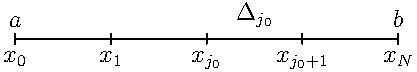
\includegraphics[height=1cm]{img/final/galat/38/T.pdf}\caption{Разбиение $T$}\label{T}
 \end{figure}
 Пусть $j_0$ "--- номер отрезка, в который добавлена новая точка.
 
 \pic{galat/38/TildeT}{1}{TildeT}{Разбиение $\widetilde T$}
 
 $s_*(\widetilde T,f)-s_*(T,f)=\inf\limits_{[x_{j_0},y]}f\cdot(y-x_{j_0})+
 \inf\limits_{[y,x_{j_0+1}]}f\cdot(x_{j_0+1}-y)-
 \inf\limits_{[x_{j_0},x_{j_0+1}]}f\cdot(x_{j_0+1}-x_{j_0})\hm\geq
 \inf\limits_{\Delta_{j_0}}f\cdot(y-x_{j_0})\hm+\inf\limits_{\Delta_{j_0}}
 f\cdot(x_{j_0+1}-y)-\inf\limits_{\Delta_{j_0}}f\cdot|\Delta_{j_0}|=0.$
 \end{Proof}
 
 \pic{galat/38/sf}{6}{sf}{Нижняя грань}
 
 \begin{Def}
 	Разбиение $\widetilde T$ отрезка $[a,b]$ называется измельчением разбиения $T$,
 	если $\widetilde T$ можно получить из $T$ добавлением конечного числа точек.
 \end{Def}
 
 \begin{Ut}\label{imel}
 	Пусть $\widetilde T$ "--- измельчение разбиения $T$. Тогда
 	\begin{itemize}
 	  \item $s_*(T,f)\leq s_*(\widetilde T,f)$;
 	  \item $S^*(T,f)\geq S^*(\widetilde T,f)$.
 	\end{itemize}
 \end{Ut}
 
 \begin{Proof}
 	Сразу следует из утверждения \ref{Razbmi} и аксиомы \ref{Induct} индукции.
 \end{Proof}
 
 \begin{Ut}
 	$\forall\  T,\widetilde T$ "--- разбиений $[a,b]$, "---
 	$s_*(T,f)\leq S^*(\widetilde T,f).$
 \end{Ut}
 
 \begin{Proof}
 	Пусть $T=\ar xj0N$, $\widetilde T=\ar{\widetilde x}j0{\widetilde N}$.
 	Рассмотрим разбиение $T_+$, содержащее все точки $\ar xj0N$ и 
 	все точки $\ar{\widetilde x}j0{\widetilde N}$ "--- объединение разбиений.
 	$T_+$ является измельчением $T$ и $T_+$ является измельчением $\widetilde T$.
 	Значит, $s_*(T,f)\leq s_*(T_+,f)\leq S^*(T_+,f)\leq S^*(\widetilde T,f)$.
 \end{Proof}
 
 \begin{Def}
 	Нижним интегралом Дарбу (ограниченной) функции $f$ на отрезке  $[a,b]$ называется число
 	$I_*=I_*(f)\hm=\sup\limits_{\substack{T\text{ "--- разб.}\\ [a,b]}}s_*(T,f)$.
 	Верхним интегралом Дарбу "--- $I^*=I^*(f)=\underset{T\text{ "--- разб. } [a,b]}{\inf S^*(T,f)}$.
 \end{Def}
 
 \begin{Ut}
 	$I_*,I^*\in\R,\pau I_*\leq I^*$.
 \end{Ut}
 
 \begin{Proof}
 	$\forall\  T,\widetilde T$ "--- разбиений отрезка $[a,b]$ 
 	$-\infty<s_*(T,f)\leq S^*(\widetilde T,f)<+\infty$. А это означает, что 
 	$\forall\ T,\widetilde T\pau s_*(T,f)$ является нижней гранью для $\big\{S^*(\widetilde T,f)\big\}$ и наоборот
 	$S^*(\widetilde T,f)$ является верхней гранью $\big\{s_*(T,f)\big\}$.
 	Допустим нашлось такое разбиение $\widetilde T$, что $S^*(T,f) < I_*$. Тогда сразу противоречие с тем, что $I_*$ точная верхняя грань. 
 	То есть $-\infty<I_*\hm\leq S^*(T,f)<+\infty$ "--- $I_*$ является какой-то нижней гранью $\big\{S^*(T,f)\big\}$. Если
 	$I_* > I^*$, то $I^*$ не является точной нижней гранью. Значит, 
 	$I_* < I^*$.
 \end{Proof}
 
 \begin{The}
 	Пусть функция $f$ ограничена на отрезке $[a,b]$. Тогда
 	$\forall\  \e>0\pau \exists\ \delta>0\colon
 	\forall\  T$ "--- разбиения отрезка $[a,b]$ с $\diam T<\delta$, "---
 	$(0\leq)I_*(f)-s_*(T,f)<\e$ и $(0\leq)S^*(T,f)-I^*(f)<\e$.
 \end{The}
 
 \begin{Proof}
 	
 \begin{Th}
 	Пусть $|f|<C$ на отрезке $[a,b]$, $\widetilde T$ "--- разбиение $[a,b]$.
 	Пусть также разбиение $T$ получается из $\widetilde T$ удалением
 	одной точки. Тогда $0\leq s_*(\widetilde T,f)-s_*(T,f)\leq 4\cdot C\cdot\diam \widetilde T$,
    $0\leq S^*(T)-S^*(\widetilde T)\hm<4\cdot C\cdot\diam \widetilde T$.	
 \end{Th}
 
 \begin{proof}
 	Пусть $T$ получается из $\widetilde T$ выкидываением точки $\widetilde x_j$.
 	Тогда $\Delta_j=\widetilde \Delta_j\cup\widetilde\Delta_{j+1}$.
 	
 	$s_*(\widetilde T)-s_*(T)=\inf\limits_{\widetilde \Delta_j}f\cdot|\widetilde\Delta_j|+
 	\inf\limits_{\widetilde\Delta_{j+1}}f\cdot|\widetilde\Delta_{j+1}|-
 	\inf\limits_{\Delta_j}f\cdot|\Delta_j|\leq C\cdot\diam \widetilde T+
 	C\cdot\diam \widetilde T+C\cdot 2\diam \widetilde T=4\diam\widetilde T\cdot C.$
 \end{proof}
 
 Зафиксируем произвольное $\e>0$. Найдём $\widetilde T=\ar{\widetilde x}j0{\widetilde N}$ "--- разбиение 
 отрезка $[a,b]\colon I_*-s_*(\widetilde T,f)<\dfrac{\e}2$\footnote{Если 
 такого разбиения нет, то $I_*-s_*(T)\geq\dfrac{\e}2\imp I_*-\dfrac{\e}2\geq s_*(T)\imp$ противоречие с тем, что $I_*$ "--- точная верхняя грань.}.
 Найдём $C>0\colon |f|\leq C$ на отрезке $[a,b]$. Положим $\delta=\min\left\{\dfrac{|\widetilde\Delta_1|}{100},
 \dfrac{|\widetilde\Delta_2|}{100},\ldots,\dfrac{|\widetilde\Delta_N|}{100},\dfrac{\e}{1024C\widetilde N}\right\}.$
 
 Пусть $T$ "--- произвольное разбиение отрезка $[a,b]$ с $\diam T<\delta$. Обозначим
 $T=\ar xj0N$. Возьмём $T_+$ "--- разбиение $[a,b]$, включающее все точки 
 $\ar{\widetilde x}j0{\widetilde N}$ и $\ar xj0N$ и только их.
 Тогда $I_*-s_*(T)=\left(I_*-s_*(\widetilde T)\right)\hm+s_*(\widetilde T)-
 s_*(T_+)+s_*(T_+)-s_*(T)\leq\dfrac{\e}2+0$\footnote{$T_+ 
 - $изменение $\widetilde T$}$+(\widetilde N-1)$\footnote{Разбиение
 $T$ получено из разбиения $T_+$ удалением не более $(\widetilde N-1)$ точки.}$\cdot4C\delta<\dfrac{\e}2+\dfrac{\widetilde N\cdot4C\cdot\e}{1024\cdot C\cdot \widetilde N}<\e.$
 \end{Proof}
 
 \section{Интегралы Римана и интегралы Дарбу}
 
 \pic{galat/39/t}{1}{t}{Разбиение}
 
 Если есть разбиение, то сразу возникает понятие интегральной суммы $\sigma(f,T,\xi)=\sum\limits_{j=1}^Nf(\xi_j)|\Delta_j|$. Чтобы не возиться с 
 суммами мы ввели пару обозначений: $m_j=\inf\limits_{x\in\Delta_j}f(x),\pau M_j=\sup\limits_{x\in\Delta_j}f(x)$.
 И у нас возникают ещё понятия $s_*(T)=\sum\limits_{j=1}^Nm_j|\Delta_j|$ "--- нижняя сумма Дарбу, и $\sum\limits_{j=1}^NM_j|\Delta_j|$ "--- верхняя сумма Дарбу.
 
 \begin{Def}
 	Интеграл Римана: $\forall\ \e>0\pau\exists$ масштаб $\delta>0\colon\forall\ \T=(T,\xi)$ (отмеченного разбиения отрезка $[a,b]$ с $\diam T<\delta$) 
 	$|\sigma(f,T,\xi)-I|<\e$.
 \end{Def}
 
 \begin{Def}
 	Интегральчики Дарбу:
 	\begin{itemize}
 	  \item Нижний: $I_*=\sup\limits_{T\text{ "--- разб.}}s_*(T)$;
 	  \item Верхний: $I^*=\inf\limits_{T\text{ "--- разб.}} S^*(T)$.
 	\end{itemize}
 \end{Def}
 
 Какие бы разбиения мы ни взяли, $s_*(T_1)\leq I_*$. Какое разбиение бы мы ни взяли, $I^*\leq S^*(T_2)$. А ещё мы установили, что $s_*(T_1)\leq I_*\leq I^*\leq S^*(T_2)$.
 
 Что ещё мы умудрились установить:
 
 \begin{The}
 	$\forall\ \e>0\pau\exists\ \delta>0\colon\forall\  T$ (разбиения отрезка $[a,b]$ с $\diam T<\delta$) 
 	\[I_*-\e\hm<s_*(T)\hm\leq I_*\hm\leq I^*\hm\leq S^*(T)<I^*+\e.\]
 \end{The}
 
 Какие отсюда можно сделать умные или не очень выводы? Перед выводами я напомню, что $s_*(T)\hm=\inf\limits_{\xi}\sigma(f,T,\xi)$, $S^*(T)=\sup\limits_{\xi}\sigma(f,T,\xi)$.
 
 \begin{The}[Критерий интегрируемости Дарбу с цифирью раз]\label{cifir1}
 	Следующие утверждения эквивалентны
 		\begin{enumerate}
 		  \item $f\in\Rim[a,b]$, ну и добавочка: (и $\ds\int\limits_a^b f\,dx=I$);
 		  \item $I_*=I^*$ ($=I$).
 		\end{enumerate}
 \end{The}
 
 Давайте его попробуем доказать, благо это недолго.
 
 \begin{Proof}
 Давайте сначала ввыведем из первого утверждения второе: пусть $f\in\Rim[a,b]$ и $\ds\int_a^bf\,dx=I$ "--- это число просто число.
 Выберем произвольное $\e>0$, найдём $\delta>0\colon\forall\ \T=(T,\xi)$ "--- отмеченного разбиения отрезка $[a,b]$ с $\diam T<\delta$, "--- 
 $|\sigma(f,T,\xi)-I|<\e$ или другими словами $I-\e<\sigma(f,T,\xi)<I+\e$. Возьмём разбиение $T$ отрезка $[a,b]$  с $\diam T<\delta$.
 Тогда $\forall$ набора $\xi$ отмеченных точек для разбиения $T$ выполняется:
 \[I-\e<\sigma(f,T,\xi)<I+\e,\] значит, $I-\e\leq\inf\limits_{\xi}\sigma(f,T,\xi)=s_*(T)\leq I_*$.
 
 Абсолютно аналогично $I+\e\geq\sup\limits_{\xi}\sigma(f,T,\xi)=S^*(T)\geq I^*$. Значит, 
 $I-\e\leq I_*\leq I^*\leq I+\e$ и это верно $\forall\  \e>0.$
 
 Написано, что \begin{align*}
 	|I_*-I|&\leq\e;\\ |I^*-I|&\leq\e;
 \end{align*}$\imp$ в силу произвольности: $\e$ $I^*=I_*$.
 
 Ну давайте теперь выведем из второго первое. Начнём с копи-паста: зафиксируем произвольное $\e>0$, найдём $\delta>0\colon
 \forall\  T$ (разбиения отрезка $[a,b]$ с $\diam T<\delta$)
 $$I-\e=I_*-\e\leq s_*(T)\leq S^*(T)<I^*+\e=I+\e.$$
 Тогда $\forall\  (T,\xi)$ "--- отмеченного разбиения отрезка $[a,b]$ с $\diam T<\delta$
 $$I-\e<s_*(T)\leq\sigma(f,T,\xi)\leq S^*(T)<I+\e,$$
 то есть $|\sigma(f,T,\xi)-I|<\e$. Мораль: $f\in\Rim[a,b]$ и $\ds\int\limits_a^b f\,dx=I$.
 \end{Proof}
 
 Конечно хороший критерий интегрируемости. Но зачем он такой нужен? Радости с этого утверждения пока никакой. Но мы продолжим это утверждение раскручивать.
 
 \begin{The}[Тоже критерий интегрируемости Дарбу, уже с цифирью два]
 	Следующие утверждения эквивалентны:
 	\begin{enumerate}
 	  \item $f\in\Rim[a,b]$;
 	  \item $\forall\ \e>0\pau\exists\ \delta>0\colon \forall\  T$ "--- разбиения отрезка $[a,b]$ с $\diam T<\delta$, "--- $S^*-s_*<\e$.
 	\end{enumerate}
 \end{The}
 
 \begin{Proof}
 	Для начала из первого утверждения докажем второе: пусть $I=\ds\int\limits_a^bf\,dx$. Тогда $I_*=I^*=I$ по уже доказанной теореме.
 	Тогда я делаю то же, что сегодня делал: $\forall\ \e>0\pau\exists\ \delta>0\colon\forall\  T$ "--- разбиения отрезка $[a,b]$ с $\diam T<\delta$ (можем применить, как для $\e$, так и для $\dfrac{\e}2$)
 	$$I^*-\dfrac{\e}2<s_*(T)\leq S^*(T)<I^*+\dfrac{\e}2.$$
 	Отсюда следует, что $S^*(T)-s_*(T)<\e$.
 	
 	Теперь давайте в другую сторону. Это ещё проще и быстрее: возьмём произвольное $\e>0$, найдём $\delta>0\colon\forall\  T$ "--- разбиения
 	отрезка $[a,b]$ с $\diam T<\delta\pau S^*(T)-s_*(T)<\e$. Пусть $T_0$ "--- какое-то разбиение отрезка $[a,b]$ с $\diam T_0<\delta$.
 	Что можем сказать про разность $I^*-I_0$?
 	$$0\leq I^*-I_*\leq S^*(T_0)-s_*(T_0)<\e.$$
 	Мы поставили вместо точных граней конктентые элементы множества и зажали разность между нулём и любым положительным числом.
 	Мораль: $I_*=I^*\imp$ уже по доказанному $f\in\Rim[a,b]$.
 \end{Proof}
 
 В плане практического применения ничем не лучше предыдущего. Но будем дальше продвигаться в правильном направлении.
 
 \begin{The}[Критерий интегрируемости Дарбу с цифирью три]
 	Следующие утверждения эквивалентны:
 	\begin{enumerate}
 	  \item $f\in\Rim[a,b]$;
 	  \item $\exists\  T_0$ "--- разбиение отрезка $[a,b]$, хоть какое-то: $S^*(T_0)-s_*(T_0)<\e$.
 	\end{enumerate}
 \end{The}
 
 \begin{Proof}
 	Почему из первого следует второе: возьмём произвольное $\e>0$. Найдём из прошлого критерия Дарбу $\delta>0\colon \forall\  T$ "--- разбиения
 	с $\diam T<\delta$, "--- $S^*(T_0)-s_*(T_0)<\e$. Осталось в качестве $T_0$ взять произвольное разбиение отрезка $[a,b]$ с $\diam T_0<\delta$.
 	
 	В другую сторону мы это конечно же и делали. Зафиксируем произвольное $\e>0$. Найдём $T_0$ "--- разбиение $[a,b]\colon S^*(T_0)-s_*(T_0)<\e$.
 	А дальше copy-paste, ровно copy-paste того, что было: тогда
 	$$0\leq I^*-I_*\leq S^*(T_0)-s_*(T_0),$$
 	прибавляем побольше, вычитаем поменьше. Таким образом $\forall\ \e>0\pau0\leq I^*-I_*<\e$. Мораль: $I^*=I_*\imp f\in\Rim[a,b]$.
 \end{Proof}
 
 Первый критерий фундаментален, он фундамент для других критериев. Второй критерий говорит о том, что из интегрируемости по Риману многое следует, но чтобы доказать
 интегрируемость по Риману через второй критерий, нам многое требуется. Третий критерия нужен как раз для тех случаев, когда нужно доказать интегрируемость
 по Риману.
 
 \begin{Zam}
 Следующие утвеждения эквивалентны:
 \begin{enumerate}
   \item $\forall\ \e>0\pau\exists\  T_0$ "--- разбиение отрезка $[a,b]\colon S^*(T_0)-s_*(T_0)<\e$;
   \item $\forall\ \e>0\pau\exists\  T_1,T_2$ "--- разбиения отрезка $[a,b]\colon S^*(T_1)-s_*(T_2)<\e$.
 \end{enumerate}
 \end{Zam}
 
 \begin{Proof}
 	Из первого второе: $T_1=T_0$ и $T_2=T_0$. Всё.
 	
 	Из второго первое: в качестве $T_0$ возьмём разбиение отрезка $[a,b]$, содержащее все точки разбиений $T_1$ и $T_2$.
 	Тогда $S^*(T_0)-s_*(T_0)\leq S^*(T_1)-s_*(T_2)$. Ведь при измельчении верхняя сумма Дарбу уменьшается, нижняя "--- увеличивается (утверждение \ref{imel}).
 \end{Proof}
 
 Как лучше понять, что это за величина? Пусть $T$ "--- какое-то разбиение отрезка $[a,b]$ ($T=\ar xj0N, \Delta_j\hm=[x_{j-1},x_j]$). Что такое $S^*(T)-s_*(T)$?
 $S^*(T)=\sum\limits_{j=1}^NM_j|\Delta_j|$,
 $$S^*(T)-s_*(T)=\sum\limits_{j=1}^NM_j|\Delta_j|-\sum\limits_{j=1}^Nm_j|\Delta_j|=\sum\limits_{j=1}^N(M_j-m_j)|\Delta_j|.$$
 
 Пусть функция $g$ определена и ограничена на отрезке $\Delta$, $M=\sup\limits_{x\in\Delta}g(x)$, $m=\inf\limits_{x\in\Delta}g(x)$
 ($M,m\in\R$, но $g$ не обязана их достичь).
 
 \begin{Def}
 	Колебинием (осцилляцией) функции $g$ на отрезке $\Delta$ называется следующая величина $\sup\limits_{t_1,t_2}\big|g(t_1)-g(t_2)\big|$.
 	Обозначается по-разному. Иногда так и пишут $\osc(g,\Delta)$. Иногда $w(g,\Delta)$, иногда $\omega(g,\Delta)$. Омегу можно путать с модулем непрерывности.
 \end{Def}
 
 \begin{Th}
 	$\osc(g,\Delta)=M-m$.
 \end{Th}
 
 \begin{Proof}
 	$\forall\  t_1,t_2\in\Delta$
 	\begin{itemize}
 	  \item Если $g(t_1)\leq g(t_2)$, то $m\leq g(t_1)\leq g(t_2)\leq M$. Значит:
 	  $$\big|g(t_1)-g(t_2)\big|=g(t_2)-g(t_1)\leq M-m;$$
 	  \item $g(t_1)\geq g(t_2)$ рассматривается аналогично.
 	\end{itemize}
 	Нам нужно доказать, что поменьше верхнюю грань мы взять не можем. Возьмём произвольное $\e>0$. Найдём $t_1\in\Delta\colon g(t_1)>M-\dfrac{\e}2$.
 	Найдём $t_2\in\Delta\colon g(t_2)<m+\dfrac{\e}2$. Тогда
 	$$\big|g(t_1)-g(t_2)\big|\geq g(t_1)-g(t_2)>M-\dfrac{\e}2-\left(m+\dfrac{\e}2\right)=M-m-\e.$$
 	То есть $\forall\ \e>0\pau\big|g(t_1)-g(t_2)\big|>M-m-\e.$
 \end{Proof}
 
 Возвращаемся к суммам Дарбу: $S^*(T)-s_*(T)=\sum\limits_{j=1}^N\osc(f,\Delta_j)|\Delta_j|$.
 
 \begin{Sl}
 	Следующие утверждения эквивалентны:
 	\begin{enumerate}
 	  \item $f\in\Rim[a,b]$;
 	  \item $\forall\ \e>0\pau\exists\  T$ "--- разбиение отрезка $[a,b]\colon\sum\limits_{j=1}^N\osc(f,\Delta_j)|\Delta_j|<\e$.
 	\end{enumerate}
 \end{Sl}
 
 Теперь мы будем эксплуатировать то, что получили.
 
 \begin{The}
 	Пусть функция $f\in C[a,b]$. Тогда $f\in\Rim[a,b]$.
 \end{The}
 
 \begin{Proof}
 	Зафиксируем произвольное $\e>0$. По теореме \ref{kg} Кантора"--~Гейне $f$ равномерно непрерывна на отрезке $[a,b]$. 
 	То есть $\exists\ \delta>0\colon \forall\  t,\tilde t\in[a,b]\colon |t-\tilde t|<\delta\pau \left|f(t)-f(\tilde t)\right|<\dfrac{\e}{b-a}$.
 	Пусть $T_0=\ar xj0N$ "--- разбиение отрезка $[a,b]$ с $\diam T_0<\delta$, где $\Delta_j=[x_{j-1},x_j](j=1..N)$. По теореме \ref{vmaxmin} Вейерштрасса
 	$m_j=\inf\limits_{\Delta_j} f=\min\limits_{\Delta_j}f\hm=f(\xi_j^{\min})$ для некоторой $\xi_{j}^{\min}\in\Delta_j$,
 	$M_j=\sup\limits_{\Delta_j} f=\max\limits_{\Delta_j}f=f(\xi_j^{\max})$ для некоторой $\xi_{j}^{\max}\in\Delta_j$.
 	При этом разница
 	$$\left|\xi_j^{\max}-\xi_j^{\min}\right|\leq|\Delta_j|<\delta\pau(\diam T_0<\delta).$$
 	Тогда 
 	$ \ds S^*(T_0)-s_*(T_0)=\sum\limits_{j=1}^N(M_j-m_j)|\Delta_j|=\sum\limits_{j=1}^N\left(f\left(\xi_j^{\max}\right)-f\left(\xi_j^{\min}\right)\right)|\Delta_j|<\sum\limits_{j=1}^N\dfrac{\e}{b-a}|\Delta_j|\hm=\dfrac{\e}{b-a}\sum\limits_{j=1}^N|\Delta_j|\hm=\dfrac{\e}{b-a}(b-a)=\e.$
 	Значит, по одному из наших критериев Дарбу $f\in\Rim[a,b]$.
 \end{Proof}
 
 Какие ещё функции заведомо хорошие?
 
 \begin{The}
 	Пусть функция $f$ монотонна на $[a,b]$. Тогда $f\in\Rim[a,b]$.
 \end{The}
 
 \begin{Proof}
 	Рассмотрим случай, когда функция неубывает: $f\nv$. Возьмём произвольное $\e>0$. Найдём $N\in\N\colon\dfrac{(b-a)\big(f(b)-f(a)\big)}{N}<\e$.
 	Пусть $T_0$ "--- равномерное разбиение отрезка $[a,b]$ на $N$ подотрезков (длины $\dfrac{b-a}N$). Тогда
 	$S^*(T_0)-s_*(T_0)\hm=\sum\limits_{j=1}^N(M_j-m_j)|\Delta_j|\hm=\dfrac{b-a}N\sum\limits_{j=1}^N(M_j-m_j)\hm=
 	\dfrac{b-a}N\sum\limits_{j=1}^N\underset{\text{монотонна}}{\left(f(x_j)-f(x_{j-1})\right)}\hm=
 	\dfrac{b-a}{N}\left(-f(x_0)+\cancel{f(x_1)}-\cancel{f(x_1)}+\ldots+f(x_N)\right)\hm=
 	\dfrac{b-a}N\big(f(b)-f(a)\big)<\e$. Мораль: $\forall\ \e>0$ найдётся разбиение, где верхняя и нижняя суммы Дарбу отличаются меньше, чем на $\e$.
 	Значит, по последнему критерию $f\in\Rim[a,b]$.
 \end{Proof}
 
 \section{Юбилейная}
 Можно задать на отрезке разбиение $T$, а можно ещё и отметить на нём точки $\xi$, получим пару $(T,\xi)$. У нас возникает
 понятие интегральной суммы $\sigma(f,T,\xi)=\sum\limits_{j=1}^Nf(\xi_j)|\Delta_j|$ и понятие интеграла
 по Риману $\ds\int\limits_a^bf\,dx=I\hm\iff \forall\ \e>0\pau\exists\ \delta>0\colon\forall\ \T=(T,\xi)$ "--- отмеченного разбиения отрезка $[a,b]$
 с $\diam T<\delta$, "--- $|\sigma(f,T,\xi)-I|<\e$.
 
 Чтобы функция была интегрируемой по Риману, она обязана быть ограниченной. Тогда появляются обозначения
 $m_j=\inf\limits_{\Delta_j}f,\pau M_j=\sum\limits_{\Delta_j}f$. И возникает такая штука:
 $\osc(f,\Delta_j)=M_j-m_j=\sup\limits_{\tilde x,\ttilde x\in\Delta_j}\left|f(\tilde x)-f(\ttilde x)\right|.$
 
 И основной результат последних, можно сказать, двух лекций:
 
 \begin{The}
 	Ограниченная функция $f\in\Rim[a,b]\iff\forall\ \e>0\pau\exists\  T$ "--- разбиение отрезка $[a,b]$
 	(я напомню $T=\ar xj0N,\Delta_j=[x_{j-1},x_j]$)$\colon\sum\limits_{j=1}^N\osc(f,\Delta_j)\cdot|\Delta_j|<\e$.
 \end{The}
 
 Мне лень напоминать, что такое сумма Дарбу, а такая формулировка у нас тоже была.
 
 С помощью этого мы доказали, что любая непрерывная функция интегрируема по Риману на отрезке и любая монотонная
 фунция $\in\Rim[a,b]$.
 
 Напомню ещё то, что было давно:
 
 \begin{Def}
 	Функция $g(t)$ называется Липшицевой на отрезке $\Delta$ (любители могут говорить «принадлежит классу Гёльер-единица», чтобы внушало),
 	если функция  $g(t)$ определена на отрезке $\Delta$ и $\exists\  C>0\colon \forall\  t,\tilde t\in\Delta\pau\big|g(t)-g(\tilde t)\big|\leq C\big|t-\tilde t\big|^1$. 
 \end{Def}
 
 Если эту степень,
 	единичку будем менять, получим как раз функции из других классов Гёльдера. Если $>1$, то неинтересно в ней все функции получатся тождественные константы. Если
 	$<1$, то интересно, но это пока слишком интересно\ldotst{} тайные знания, они на следующем уровне. 
 
 Забыли интеграл\ldotst{} минут на пять. Какие у нас есть Липшицевы функции? Пусть $\Delta$ "--- произвольный отрезок. Тогда функция $|t|$ Липшицева на $\Delta$
 (и константа Липшица $C=1$). Что здесь написано: $\big| |t|-|\tilde t|\big|\leq\big|t-\tilde t\big|$. Надо доказывать?
 Я ещё напомню, что если функция $h\in C^1(\Delta)$\footnote{Первая производная на отрезке $\Delta$ существует и непрерывна.}, то $h$ Липшицева на $\Delta$.
 Ведь в этом случае $h'\in C(\Delta)\imp h'$ ограничена на $\Delta$ (по теореме \ref{vogr} Вейерштрасса), то есть
 $\exists\  C>0\colon |h'|\leq C$ на $\Delta$. Тогда $\forall\  t,\tilde t\in\Delta\pau\big|h(t)-h(\tilde t)\big|\underset{\substack{\text{\ref{Lag}}\\ \exists\ \xi\in\Delta}}= 
 h'(\xi)|t-\tilde t|\leq C|t-\tilde t|$.
 
 Мораль, ну какая мораль: $\sin x$ Липшицева, $x^2$ Липшицева на любом отрезке, не на всей числовой прямой сразу. А на каждом отрезке её производная $2x$ непрерывна.
 
 \begin{Th}
 	Пусть функция $f\colon\underset{\text{опр.}}{\Delta}\to[c,d]$, а функция $g$ Липшицева на $[c,d]$ с константой Липшица $C$. Тогда $\osc\Big(g\big(f(t)\big),\Delta\Big)\leq
 	C\cdot\osc(f,\Delta)$.
 \end{Th}

 \begin{Proof}
 	$\forall\  t,\tilde t\in\Delta\pau\Big|g\big(f(t)\big)-g\big(f(\tilde t)\big)\Big|\leq C\cdot\Big|f(t)-f(\tilde t)\Big|\leq
 	C\cdot \osc(f,\Delta)\imp\osc\Big(g\big(f(t)\big),\Delta\Big)\hm=\sup\limits_{t,\tilde t\in\Delta}
 	\Big|g\big(f(t)\big)-g\big(f(t)\big)\Big|\leq C\cdot\osc(f,\Delta)$.
 \end{Proof}
 
 Зачем нам это нужно собственно, это лемма к какой теореме?
 
 \begin{The}
 	Пусть функция $f\in\Rim[a,b]$ и $\forall\  x\in[a,b]\pau f(x)\in[c,d]$ (такой отрезок найдётся, ведь если интегрируема, значит, ограничена).
 	Пусть также $g$ Липшицева на $[c,d]$. Тогда $g\big(f(x)\big)\in\Rim[a,b]$.
 \end{The}
 
 \begin{Proof}
 	Как обычно: зафиксируем произвольное $\e>0$. Обозначим коконстанту Липшица функции $g$ на отрезке $[c,d]$ через $C$ ($C>0$).
 	Используем критерий Дарбу для $\e_1=\dfrac{\e}C$: найдём $T$ "--- разбиение отрезка $[a,b]\colon\sum\limits_{j=1}^N\osc(f,\Delta_j)|\Delta_j|<\e_1=\dfrac{\e}{C}$.
 	Тогда $\sum\limits_{j=1}^N\osc\Big(g\big(f(\cdot)\big),\Delta_j\Big)\cdot\big|\Delta_j\big|\hm\leq\sum\limits_{j=1}^NC\cdot\osc(f,\Delta_j)|\Delta_j|\hm<C\cdot\dfrac{\e}C=\e$.
 	Мы таким образом доказали по критерию Дарбу, что $g\big(f(\cdot)\big)\in\Rim[a,b]$.
 \end{Proof}
 
 Мощная теорема, но нам пока понадобится только один маленький кусок.
 
 \begin{Sl}[Один]
 	Если $f\in\Rim[a,b]$, то $|f|\in\Rim[a,b]$. Ещё говорят абсолютно интегрируема.
 \end{Sl}
 
 \begin{Sl}[Два]
 	Если $f\in\Rim[a,b]$, то $f^2\in\Rim[a,b]$ (как и $f^3$ и ещё что-нибудь).
 \end{Sl}
 
 \begin{Sl}[Три]\label{treee}
 	Если функции $f,g\in\Rim[a,b]$, то $(f\cdot g)\in\Rim[a,b]$.
 \end{Sl}
 
 \begin{Proof}
 	$f\cdot g=\dfrac{(f+g)^2-f^2-g^2}2$.
 \end{Proof}
 
 О чём же дальше пойдёт речь? Сейчас сначала про мотивацию: критерий Дарбу "--- хорошая штука, очень удобно использовать её в доказательствах.
 Но критерий Дарбу требует конструктивного простроения ещё одного объекта "--- разбиения. А хочется доказывать интегрируемость функции
 в терминах самой функции. Можно искать в моих словах жульничество, но на первый взгляд незаметно. Это всё была мотивация номер раз.
 Следующая мотивация: мы получили отличный результат, что композиция двух функций, из которых внутренняя интегрируема, а внешняя Липшицева, интегрируема на отрезке. Но мы ничего не
 знаем о ситуации, когда внешняя функция $\sqrt x$, $\arcsin x$, наших теорем не хватает.
 
 Пусть $A\subset \R$ (обычное подмножество $\R$).
 \begin{Def}
 	Множество $A$ имеет меру $0$ по Лебегу\footnote{Фамилия Лебег и правда склюняется, но в учебниках пишут несколько иначе: либо «имеет меру Лебега $0$», либо «имеет меру~$0$ в~смысле Лебега».},
 	 если $\forall\ \e>0\pau\exists$ не более чем счётная совокупность интервалов $\big\{l_j\big\}_j$, 
 	покрывающая $A$ (то есть $A\subset\bigcup\limits_{j}l_j$), такая, что $\sum\limits_j l_j<\e$. 	
 \end{Def}
 
 Это тот случай, когда если слово «интервалов» заменить на слово «промежутков», то ничего не изменится. Если есть совокупность интервалов,
 то можно их дополнить до любого вида промежутков, не меняя их дл\'{и}ны. Если есть совокупность отрезков для любого $\e>0$, то можно зафиксировать
 $\e>0$ и найти совокупность отрезков такую, что $\sum\limits_j \Delta_j<\dfrac{\e}2$. Покрыть каждый отрезок интервалом вдвое большей длины.
 
 Чтобы вы почувствовали, какой это экзотический объект, я приведу несколько примеров.
 \setcounter{Ut}{-2}
 \begin{Ut}[Даже на нулевое не тянет]
 	$\q$ "--- множество меры $0$ по Лебегу. Примерно такое же по мощности утверждение: одноточечное множество "--- множество меры $0$ по Лебегу.
 \end{Ut}
 \setcounter{Ut}{0}
 \begin{Ut}[Более содержательное]
 	Любое не более чем счётное множество "--- множество меры $0$ по Лебегу.
 \end{Ut}
 
 \begin{Proof}
 	Пусть множество $A=\big\{t_j\big\}$ "--- не более чем счётное множество\footnote{Договоримся нумеровать точки, начиная с $j=1$.}. Зафиксируем произвольное $\e>0$. Положим 
 	$l_j=\left(t_j-\dfrac{\e}{2^{j+2}},t_j+\dfrac{\e}{2^{j+2}}\right)$. Главное, что $t_j\in l_j$ и что $\big|l_j\big|=\dfrac{\e}{2^{j+1}}$.
 	Тогда есть неболее чем счётная система интевальчиков $\big\{l_j\big\}$, покрывающая множество $A\colon\sum\limits_j\dfrac{\e}{2^{j+1}}=\e\left(\dfrac14+\dfrac18+\dfrac1{16}+\ldots\right)=\dfrac{\e}2<\e$.
 \end{Proof}
 
 Что мы сейчас доказали? Вот например на отрезке $[0,1000]$ куда ни посмотри, в любом подотрезке найдётся хоть одна рациональная точка. А оказывается, их так мало, что все можно покрыть не 
 более чем счётной системой интервало, да ещё и сумма их длин будет меньше, чем одна миллионная. Отдельный вопрос: как так? Ну вот так. Так жизнь устроена.
 
 \begin{Ut}
 	Не более чем счётное объединение множеств меры $0$ по Лебегу "--- множество меры $0$ по~Лебегу.
 \end{Ut}
 
 \begin{Proof}
 	Я идею доказательства расскажу. Фиксируем произвольное $\e>0$. Первое множество покрываем не более чем счётной системой множеств
 	с суммой длин $<\dfrac{\e}4$, второе "--- $<\dfrac{\e}8$, третье "--- $<\dfrac{\e}{16}$,\ldotst{} 
 \end{Proof}
 
 Класс множеств меры $0$ по Лебегу существенно шире класса не более чем счётных множеств. Например, множество Кантора.
 
 \begin{Ut}
 	Подмножество множества меры $0$ по Лебегу "--- множество меры $0$ по~Лебегу.
 \end{Ut}
 
 \begin{Def}\label{BEST}
 	Говорят, что свойство выполнено почти всюду на множестве $E\in\R$, если оно выполнено во всех точках множества $E$ за исключением
 	точек, образующих множество меры $0$ по Лебегу (то есть множество точек $E$, для которых свойство не выполнено, имеет меру $0$ по Лебегу).
 \end{Def}
 
 В таких терминах: почти все числа иррациональны, почти все числа трансцентдентны, почти все точки отрезка $[0,1]$ не принадлежат множеству Кантора.
 
 \begin{The}
 Функция $f$ интегрируема по $\Rim$ на отрезке $[a,b]$, если и только если $f$ ограничена на $[a,b]$ и непрерывна почти всюду на $[a,b]$.
 То есть множество точек разрыва $f$ на $[a,b]$ имеет меру $0$ по~Лебегу.
 \end{The}
 
 Специально для любителей коротких формулировок: если говорить $f\in\Rim[a,b]\iff f$ ограничена и непрерывна почти всюду на отрезке, то это правильно.
 Но надо только ещё правильно понимать эту формулировку: функция должна быть ограничена всюду на отрезке, а разрывы иногда разрешаются.
 
 С помощью последней теоремы можно было вывести половину следствий из тех, что мы уже вывели. Но это было бы нечестно, потому что доказывать эту теорему
 мы не будем.
 
 \begin{Sl}[Только неважное следствие]
 	Пусть функция $f\in\Rim[a,b]$ и $\forall\  x\in[a,b]\pau f(x)\in[c,d]$. Пусть также $g\in C\big([c,d]\big)$. Тогда сложная функция $g\big(f(x)\big)\in\Rim[a,b]$.
 \end{Sl}
 
 \begin{The}
 	Пусть $f\in\Rim[a,b]$, $c\in(a,b)$. Тогда $f\in\Rim[a,c]$ и $f\in\Rim[c,b]$.
 \end{The}
 
 \begin{Proof}
 	Зафиксируем произвольное $\e>0$. Найдём разбиение $\widetilde T$ отрезка $[a,b]\colon S^*(\widetilde T,f)-s_*(\widetilde T,f)<\e$.
 	Получим разбиение $T$ отрезка $[a,b]$ из разбиения $\widetilde T$ добавлением точки $c$. Тогда $S^*(T,f)-s_*(T,f)<\e$ (утверждение \ref{imel}).
 	Я не буду говорить лишних слов, обозначения сразу на рисунке.
 	\pic{galat/40/Tar}{0.75}{TAR}{Обозначения}
 	Тогда точки множества $T_{\rus{л}}=\big\{x_0,\ldots,x_k\big\}$ образуют разбиение отрезка $[a,c]$, причём
 	$S^*(T_{\rus{л}},f)-s_*(T_{\rus{л}},f)\hm=\sum\limits_{j=1}^k\osc(f,\Delta_j)|\Delta_j|\hm\leq\sum\limits_{j=1}^N\osc(f,\Delta_j)|\Delta_j|\hm=
 	S^*(T,f)-s_*(T,f)<\e$. Следовательно в соответствии с критерием Дарбу $f\in\Rim[a,c]$. Абсолютно аналогично доказывается, что $f\in\Rim[c,b]$.
 \end{Proof}
 
 \begin{Sl}
 	Пусть $f\in\Rim[a,b]$ и $[c,d]\subset[a,b]$. Тогда $f\in\Rim[c,d]$.
 \end{Sl}
 
 Если одновременно два человека хорошие, то каждый по отдельности тоже хороший. А если оба хорошие по-отдельности и их собрали вместе?
 
 \begin{The}[Об аддитивности интаграла Римана на отрезке]\label{AddiRim}
 	Пусть $a<c<b$, $f\in\Rim[a,c]$ и $f\in\Rim[c,b]$. Тогда $f\in[a,b]$, причём $\ds\int\limits_a^bf\,dx=\int\limits_a^cf\,dx+\int\limits_c^bf\,dx$.
 \end{The}
 
 \begin{Proof}
 	Давайте как-нибудь карявенько это докажем и успокоимся. Пусть $I_1=\ds\int\limits_a^cf\,dx$, $I_2=\ds\int\limits_c^bf\,dx$.
 	Я~пишу, функция $f$ ограничена и на $[a,c]$, и на $[a,b]$. Значит, $\exists\  C>0\colon|f|<C$ на всём отрезке $[a,b]$.
 	Поехали дальше: зафиксируем произвольное $\e>0$. Найдём $\delta_1>0\colon\forall\ (T,\xi)$ "--- отмеченного разбиения отрезка $[a,c]$
 	с~$\diam T<\delta_1$, "--- $\big|\sigma(f,T,\xi)-I_1\big|<\dfrac{\e}3$.
 	Найдём $\delta_2>0\colon\forall\ (T,\xi)$ "--- отмеченного разбиения $[c,b]$  с~$\diam T<\delta_2$, "--- 
 	$\big|\sigma(f,T,\xi)-I_2\big|<\dfrac{\e}3$.
 	Положим $\delta=\min\left\{\delta_1,\delta_2,\dfrac{\e}{10C}\right\}$.
 	Пусть $(T,\xi)$ "--- произвольное отмеченное разбиение отрезка $[a,b]$ с~$\diam T<\delta$.
 	Точка $c$ могла и не попасть в разбиение: пусть $\widetilde T$ "--- разбиение отрезка $[a,b]$, полученное из $T$ добавлением точки $c$.
 	Пусть $\tilde \xi$ "--- набор отмеченных точек, полученных из $\xi$ произвольным изменением точек в~отрезках, содержащих $c$.
 	Отметим, что $\big|\sigma(f,T,\xi)-\sigma(f,\widetilde T,\xi)\big|\underset{\substack{3\text{ "--- число}\\ \text{потенциально}\\ \text{разных}\\ \text{слагаемых}}}{<3\cdot C\cdot \delta\leq}\dfrac{3\cdot C\cdot\e}{10\cdot C}<\dfrac{\e}3$.
 	
 	У нас $(\widetilde T,\widetilde \xi)$ содержит $\T_{\rus{л}}$, отмеченное разбиение $[a,c]$ с $\diam\T_{\rus{л}}<\delta_1$, и
 	$\T_{\rus{п}}$, отмеченное разбиение отрезка $[c,b]$ с $\diam\T_{\rus{п}}<\delta\leq\delta_2$.
 	Тогда $\big|\sigma(f,T,\xi)-(I_1+I_2)\big|\hm\leq\big|\sigma(f,T,\xi)-\sigma(f,\widetilde T),\widetilde \xi\big|+
 	\big|\sigma(f,\widetilde T,\widetilde\xi)-(I_1+I_2)\big|\hm<\dfrac{\e}3+\underbrace{\big|\sigma(f,\T_{\rus{л}}-I_1)\big|}_{<\frac{\e}3}+
 	\underbrace{\big|\sigma(f,\T_{\rus{п}})-I_2\big|}_{<\frac{\e}3}<\e$.
 \end{Proof}
 
 \section{Приложения интеграла Римана}
 
 Продолжаем обсуждать базовые вещи. Мы помним, что любая непрерывная или любая монотонная на~отрезке функция интегрируема на этом отрезке. Значение функции в конечном числе точек не влияет на интеграл.
 И~что если функция интегрируема на~отрезке, то интегрируема на его кусочках. И наоборот: если интегрируема на частях отрезка, то
 интегрируема на всём отрезке. Давайте сделаем из этого какие-то бесплатные следствия.
 
 \begin{Def}
 	Функция $f$ кусочно непрерывна на отрезке $[a,b]$, если она непрерывна на $[a,b]$ всюду, за~исключением
 	конечного набора точек, в которых у $f$ устранимые разрывы или разрывы первого рода (рисунок~\ref{urpr}).
 	
 	\pic{galat/41/01}{2}{urpr}{Кусочно непрерывная функция}
 	
 	Иными словами: $f$ кусочно непрерывна на отрезке $[a,b]$, если $\exists$ разбиение отрезка $[a,b]$ на конечный набор
 	непересекающихся подотрезков $\Delta_1,\ldots,\Delta_N\colon\forall\  j\in\{1..N\}\pau f$ можно
 	доопределить или переопределить в концах отрезка $\Delta_j$ так, что $f$ станет непрерывна на всех подотрезках $\Delta_j$.
 \end{Def}
 
 Интегрируемость функции терпит в концах подотрезков какие-то проблемы, но не любые. Фукнкция всё же должна быть 
 всюду ограничена на отрезке и разрыв второго рода интегрируемость не сохранит.
 
 \begin{Ut}
 	Если функция $f$ кусочно непрерывна на отрезке $[a,b]$, то $f\in\Rim[a,b]$.
 \end{Ut}
 
 Точно такие же слова можно сказать про «кусочно монотонные»:  $f$ кусочно монотонна на отрезке $[a,b]$, если $\exists$ разбиение отрезка $[a,b]$ на конечный набор
 	непересекающихся подотрезков $\Delta_1,\ldots,\Delta_N\colon\forall\  j\in\{1..N\}\pau f$ можно
 	доопределить или переопределить в концах отрезка $\Delta_J$ так, что $f$ станет монотонна на всех подотрезках $\Delta_j$.
 	
 	\begin{The}[Первая теорема о среднем\footnote{В дифференциальном исчислении уже были теоремы (Ролля: \ref{Roll}, Лагранжа \ref{Lag}, Коши \ref{Kohi}) о среднем.}]
 	\label{FirTheMid}Может быть, первая и единственная, может и не единственная. Формулировать дольше, чем доказывать. Пусть $f,g\in\Rim[a,b], g\geq0$ на $[a,b]$. Тогда
 	$\exists\  C\colon\inf\limits_{[a,b]}f(x)\leq C\leq \sup\limits_{[a,b]}f(x)$ и
 	$$\ds\int\limits_a^bf(x)g(x)\,dx=C\cdot\int\limits_a^bg(x)\,dx.$$
 	Интеграл произведения равен интегралу неотрицательной функции умножить на, вот проблема, как обычно неизвестную константу.
 	\end{The}
 	
 	\begin{Proof}
 	На всякий случай: мы действительно имеем право говорить об интеграле произведения, мы доказали следствие \ref{treee}.
 	Обозначим $\inf\limits_{[a,b]}f(x)$ через $m$, $\sup\limits_{[a,b]}f(x)$ через $M$. Я замечу, что функция $f$ огрпничена на $[a,b]$ по необходимому
 	условию интегрируемости (утверждение \ref{Rimneob}). Значит, $m,M\in\R$. Это комментарий о~том, что здесь бесконечностей нет.
 	
 	На отрезке $[a,b]\pau m\leq f(x)\leq M$. Домножим это неравенство на $g(x)$, она у нас всюду неотрицательна:
 	
 	$$m\cdot g(x)\leq f(x)\cdot g(x)\leq M\cdot g(x).$$
 	Теперь возьмём и проинтегрируем. Интеграл "--- предел, правда частичных сумм, но всё же сохраняющий
 	нестрогие неравенства (следствие \ref{Rimnestr} или прямо утверждение \ref{Basanestr}):
 	$$m\cdot\int\limits_a^bg(x)\,dx\leq\int\limits_a^bf(x)\cdot g(x)\,dx\leq M\cdot\int\limits_a^bg(x)\,dx\text{ "---}$$
 	это неравенства чисел, не функций. $g\geq0\imp \ds\int\limits_a^bg(x)\,dx\geq0$. Тогда два случая:
 	
 	\begin{enumerate}
 	  \item Если $\ds\int\limits_a^bg(x)\,dx=0$, то имеем $0\leq\ds\int\limits_a^bf(x)\cdot g(x)\,dx\leq 0$. За $C$ можно взять
 	  всё, что угодно: хотите $c=m$, хотите $C=M$, хотите самое настоящее среднее $C=\dfrac{m+M}2$;
 	  \item Второй случай тоже более-менее тривиальный: $\ds\int\limits_a^bg(x)\,dx>0$, поделим на эту положительную величину:
 	  $$m\leq\dfrac{\int\limits_a^bf g\,dx}{\int\limits_a^bg\,dx}\leq M,$$
 	  это число и обозначу через $C$. И всё.
 	\end{enumerate}
 	\end{Proof}
 	
 	Эта теорема приоблетает более приятный вид, если на $f$ положить дополнительные ограничения. Например непрерывность:
 	
 	\begin{Sl}
 		Пусть $g\in\Rim[a,b],g\geq0$ на $[a,b]$, $f\in C[a,b]$ (то она точно интегрируема). Тогда
 		$$\exists\  c\in[a,b]\text{ (это уже агрумент)}\colon\int\limits_a^bf(x)\cdot g(x)\,dx=f(c)\cdot\int\limits_a^bg(x)\,dx.$$
 	\end{Sl}
 	
 	Следствие следует из только что доказанной первой теоремы о среднем и теоремы \ref{bk} о промежуточных значениях для непрерывной функции.
 	В основных теоремах дифференциального исчисления были б\'{о}лее средние, из интервала $(a,b)$. Здесь тоже можно немножко поковыряться и 
 	получить такой результат. И это будет обязательная задача к коллоквиуму.
 	
 	Можно ещё упростить. Наример: $g\equiv1$.
 	
 	\begin{Sl}
 		Если $f\in C[a,b]$, то $\exists\  c\in[a,b]\colon \ds\int\limits_a^bf(x)\,dx=f(x)\cdot(b-a)$.
 	\end{Sl}
 	
 	\subsection{Мотивировочная часть}
 	Зачем нам эти интегралы нужны. Если выйти на улицу, какую-нибудь отличную от улицы Хохлова, за~биофак, и провести
 	опрос «что такое интеграл», многие ответят, что интеграл "--- это площать. Даже многие магистры и даже магистры мех-мата, есть даже такие люди.
 	Это примерно площадь, но не до конца строго. У нас вообще разговор о~площади не~до~конца строгий. Ибо нет строгого понятия «площадь».
 	Пока я занимаюсь непрекрытым обманом. Будем считать, что «какой дурак не знает, что такое площадь». Все прекрасно помним, как найти
    площадь Ленина: длину Ленина умножить на ширину Ленина.
    
    \begin{The}
    Пусть $f\in C[a,b]$ и $f\geq0$ на $[a,b]$. Тогда площадь криволинейной трапеции 
    $$\big\{(x,y)\colon x\in[a,b], 0\leq y\leq f(x)\big\}
    \text{ просто таки равна }\ds\int\limits_a^bf(x)\,dx.$$
    \end{The}
    
    
    \begin{figure}[tbp]%Бьюсь, чтобы доказательство теоремы \ref{DDK} было на одной странице. Скорее всего просто img/final/galat/41/03.pdf перерисую.
		\centering
		\begin{minipage}{0.45\textwidth}
			\centering
			\hspace*{-2em}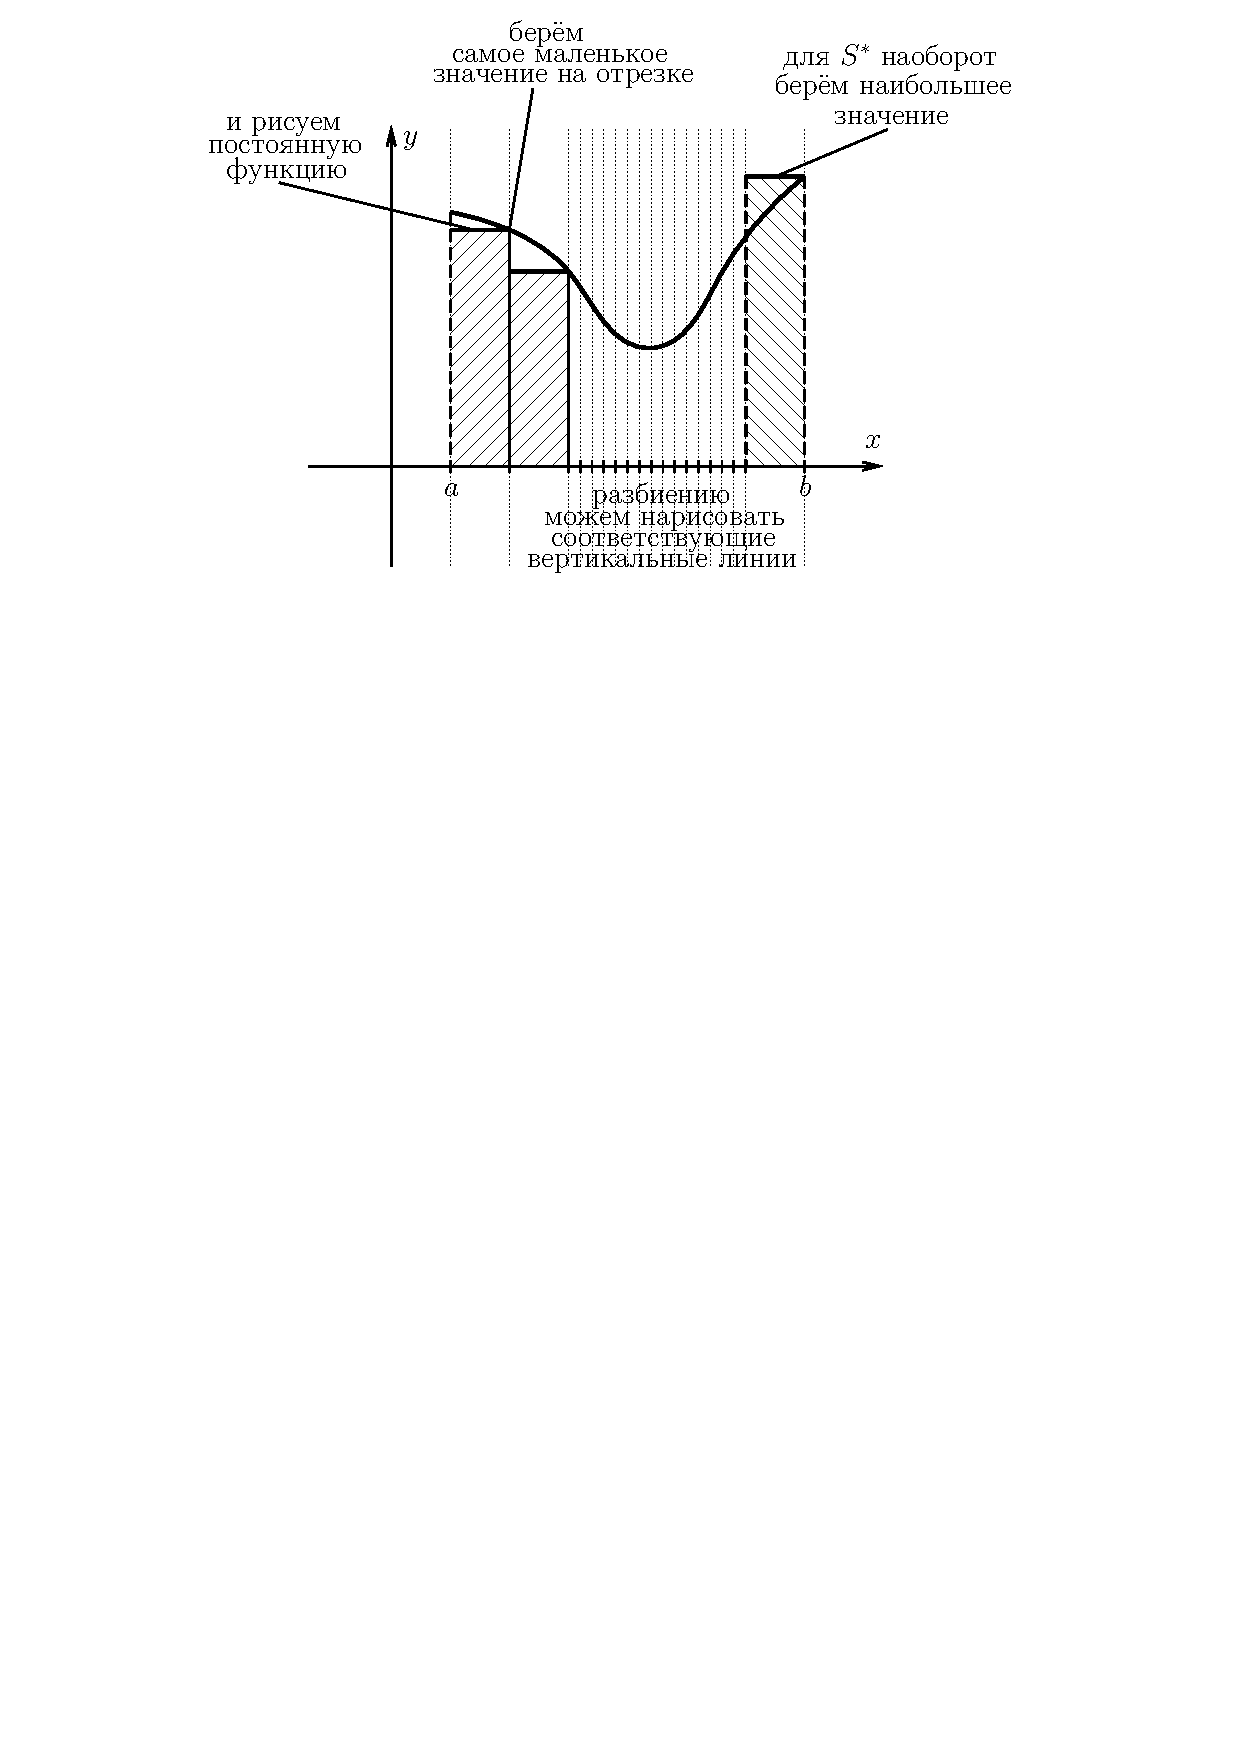
\includegraphics[height=6.5cm]{img/final/galat/41/02.pdf}
			\caption{Площадь криволинейной трапеции}
			\label{krivotrap}
		\end{minipage}\quad
		\begin{minipage}{0.45\textwidth}
			\centering
			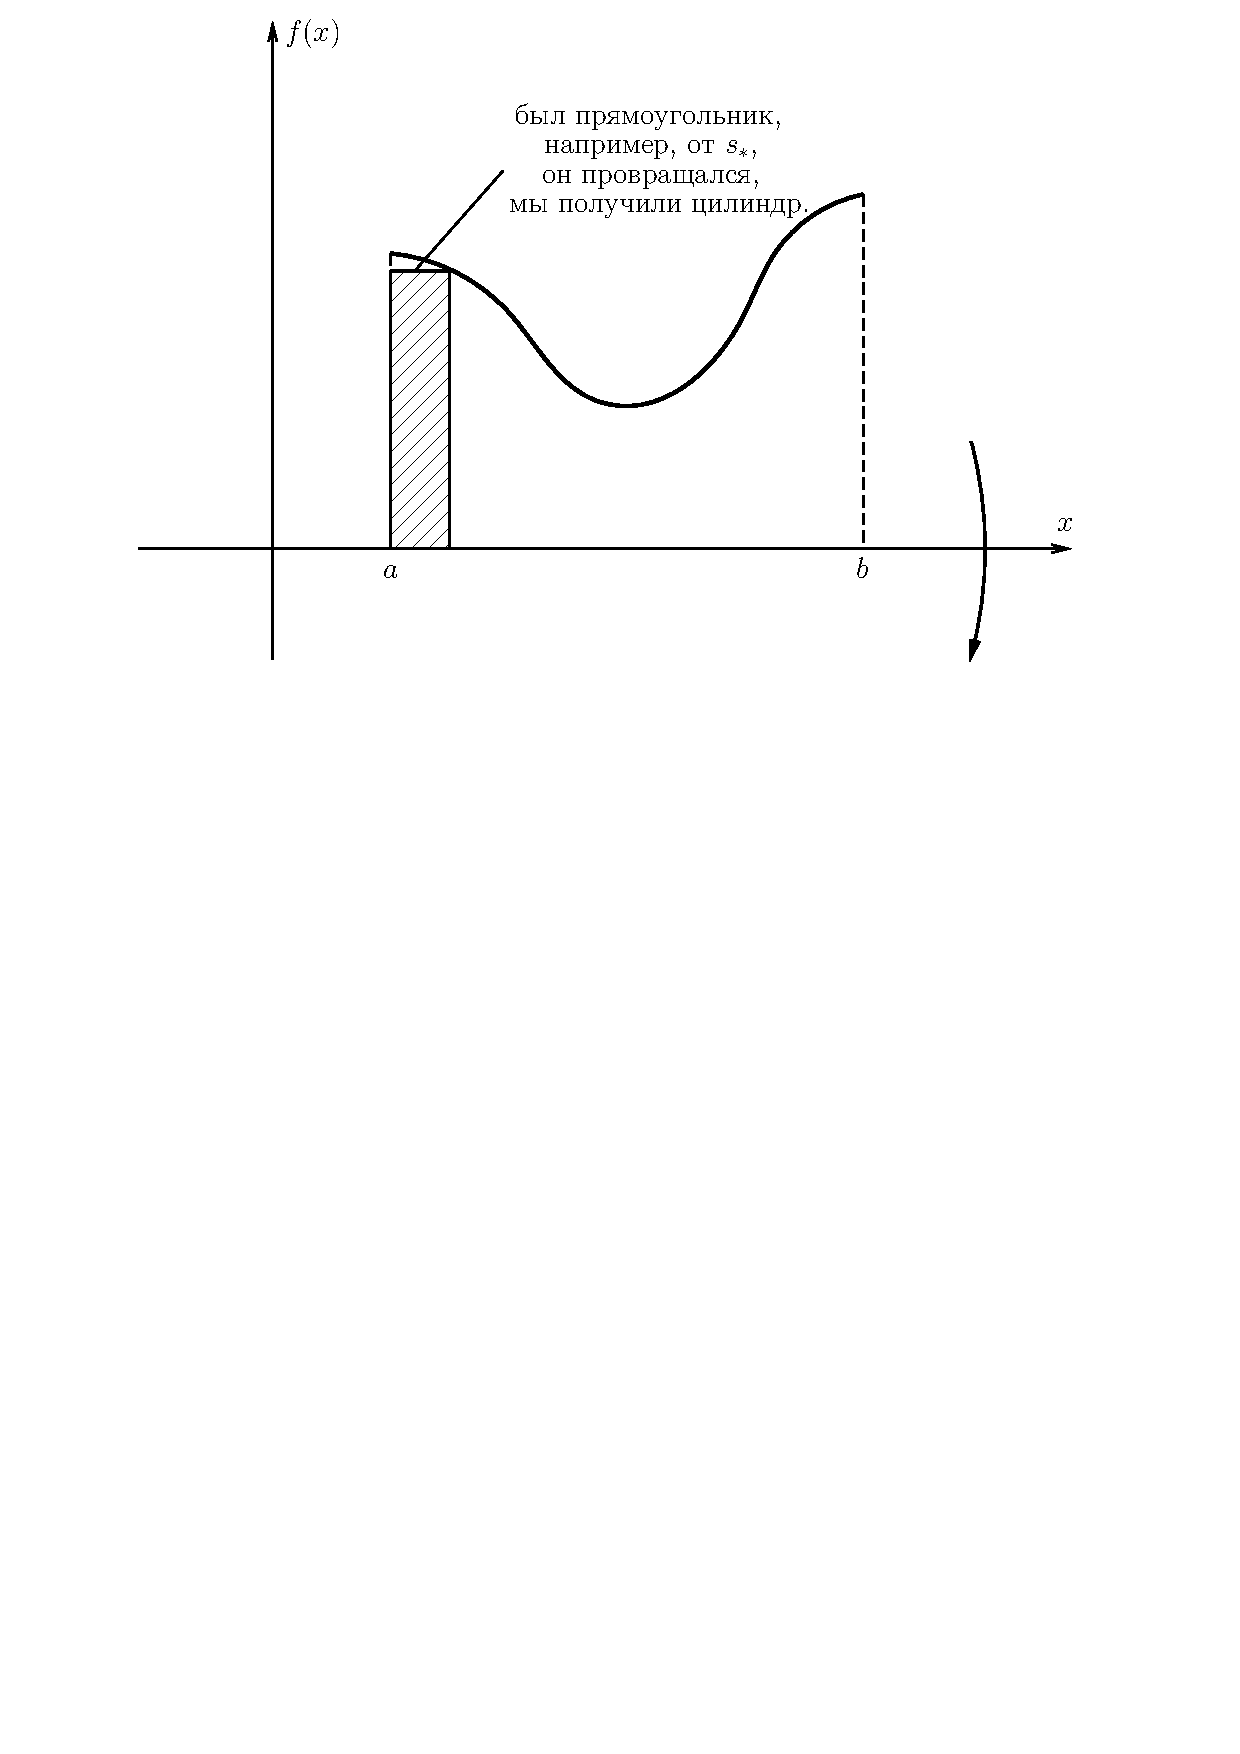
\includegraphics[height=6cm]{img/final/galat/41/03.pdf}
			\caption{Объём тела вращения}
			\label{telovrash}
		\end{minipage}
	\end{figure}
    
    \begin{Proof}
    	Как показать, что её площадь $S$ в точности равна интегралу? Пусть $T$ "--- произвольное разбиение отрезка $[a,b]$.
    	Тогда $s_*(T,f)$ "--- площадь кусочно прямоугольной фигуры, вложенной в криволинейную трапецию, а $S^*(T,f)$
    	"--- площадь кусочно прямоугольной фигуры, содержащей криволинейную трапецию (рисунок \ref{krivotrap}).
    	Мы конечно не знаем, что такое площадь, но мы же понимаем, что $s_*<S^*$. Значит, для любого разбиения $T$ $s_*(T)\leq S\leq S^*(T)$.
    	Мораль: $I_*\leq S\leq I^*$. Всё, что осталось следать, вспомнить критерий \ref{cifir1} Дарбу: $I_*=I^*=I$.
    \end{Proof}
    
    \begin{The}
    	Пусть $f\in C[a,b], f\geq 0$ на $[a,b]$. Тогда объём тела вращения
    	$$\big\{(x,y,z)\colon x\in[a,b], y^2+z^2\leq f^2(x)\big\}\text{ равен } \pi\cdot\int\limits_a^bf^2(x)\,dx.$$
    \end{The}
    
    Для любителей строгости эта теорема ещё хуже предыдущей. Мало того, что мы не знаем, что такое объём, так тут ещё и число $\pi$. Но функцию
    $\sin$ мы вводили? Ну и хорошо.
    
    \begin{Proof}
    	Аналогично (зажимаем между цилиндрическими телами, рисунок \ref{telovrash}).
    	Объём первого цилиндра: $\pi m_1^2|\Delta_1|$ "--- первое слагаемое $s_*(f^2)$. Абсолютно аналогично $\pi m_2^2|\Delta_2|$.
    	$$s_*(f^2)\leq \pi f^2\leq S^*(f^2).$$
    \end{Proof}
    
    Следующая вещь тоже не очень формально. Ещё одно приложение.
    
    \pic{galat/41/04}{1}{sterjen}{Стержень}
    
    Стержень. Можем ввести понятие линейной плотности $\rho(x)=\lim\limits_{\e\to0+}\dfrac{\text{масса стрержня $[x-\e,x+\e]$}}{2\e}$.
    Какие лёгкие свойства можем понять?
    
    \begin{The}
    	Пусть плотность стержня $\rho(x)$ при $x\in[a,b]$ кусочно непрерывна. Тогда масса стержня просто равна $\ds\int\limits_a^b\rho(x)\,dx$.
    \end{The}
    
    \begin{Proof}
    	Краткая версия доказательства: «аналогично». Менее краткая версия: пусть $\mu$ "--- масса стержня, $T$ "--- произвольное
    	разбиение $[a,b]$. Тогда $s_*(T,\rho)$ "--- масса стержня с кусочно постоянной плотностью $\leq \rho$, а 
    	$S^*(T,\rho)$ "--- масса стержня с кусочно постоянной плотностью $\geq\rho$.
    	
    	\pic{galat/41/05}{1}{Sterjen}{Разбитый стержень}
    	Значит, $\forall$ разбиения $T$ отрезка $[a,b]\pau s_*(T)\leq \mu\leq S^*(T)\imp$ как обычно
    	$I_*(T)\leq\mu\leq I^*(T)$, а это обычный интеграл Римана.
    \end{Proof}
    
    \subsection{Длина дуги кривой}
    Можно обсудить площадь поверхности тела вращения. Но это совсем грустно: мы не знаем, что такое площадь на плоскости.
    Но ещё одно приложение мы всё-таки обсудим. И здесь в отличие от предыдущего я~дам все необходимые определения. Знаете:
    длина отрезка $\sqrt{(x_1-x_2)^2+(y_1-y_2)^2}$.
    
    Пусть $f(x)\in C[a,b]$. Рассмотрим множество множество (кривую):
    $$l=\big\{(x,y)\colon x\in[a,b], y=f(x)\big\}.$$
    Каждому разбиению $T$ отрезка $[a,b]$ соответствует ломаная, которую я обозначу через $L(T)$, вписанная в эту кривую.
    
    \pic{galat/41/06}{6}{Duga}{Ломаная, вписанная в кривую}
    Получаем ломаную, а что такое длина ломаной, мы знаем.
    
    \begin{Def}
    	Длиной кривой $l$ называется $\sup\limits_{\substack{T\text{ "--- разб.}\\ [a,b]}}L(T).$
    \end{Def}
    
    \begin{The}\label{DDK}
    	Пусть $f\in C^1[a,b]$. Тогда длина $d$ кривой $l$ равна $\ds\int\limits_a^b\sqrt{1+f'^2(x)}\,dx$.
    \end{The}
    
    \begin{Proof}
    	Отметим сначала, что при измельчении разбиения, длина вписанной ломаной не уменьшается (неравенство
    	треугольника же есть).
    	Пусть $T=\{x_0,x_1,\ldots,x_N\}$ "--- произвольное разбиение нашего отрезка $[a,b]$.
    	Что будет представлять длина ломаной:
    	$$L(T)=\sum\limits_{j=1}^N\sqrt{(x_{j-1}-x_j)^2+\big(f(x_{j-1})-f(x_j)\big)^2}.$$
    	По теореме \ref{Lag} Лагранжа $\exists\  \xi\in\Delta_J\colon$
    	$$L(T)=\sum\limits_{j=1}^N\sqrt{(x_{j-1}-x_j)^2+\big(f'(\xi_j)\cdot(x_{j-1}-x_j)\big)^2}.$$
    	Ну а теперь давайте просто из-под корня вынесем $\big|(x_{j-1}-x_j)\big|$ "--- это же $|\Delta_j|$:
    	$$L(T)=\sum\limits_{j=1}^N|\Delta_j|\cdot\sqrt{1+\big(f'(\xi_j)\big)^2}=\sigma\left(\sqrt{1+f'^2(x)},T,\xi\right).$$
    	Из этого следует, что $\forall$ разбиения $T$
    	$$L(T)\leq\max\limits_{[a,b]}\sqrt{1+f'^2(x)}\cdot(b-a)<+\infty.$$
    	Значит, длины всех ломаных ограничены одной и той же константой, значит, $d<+\infty$\footnote{Функция
    	$f(x)=\begin{cases}
    		x\sin\frac1x,&x\neq0;\\ 
    		x,&x=0.
    	\end{cases}$ "--- замечательная непрерывная кривая, даже график какой-то есть, а длина дуги равна $+\infty$.
    	Здесь важно существование непрерывной производной.}.
    	
    	Зафиксируем произвольное $\e>0$. Найдём $\widetilde T$ "--- разбиение $[a,b]\colon d-\dfrac{\e}2<L(\widetilde T)\leq d$,
    	$d$ "--- это же точная верхняя грань. Поехали дальше: найдём такую величину $\delta>0$, что 
    	$\forall$ отмеченного разбиения   $(T,\xi)$ отрезка $[a,b]$ с~$\diam T<\delta$
    	\[\bigg|\sigma\left(\sqrt{1+f'^2(x)},T,\xi\right)-\ds\underbrace{\int\limits_a^b\sqrt{1+f'^2(x)}\,dx}_{I}\bigg|<\dfrac{\e}2.\]
    	Получим  разбиение $T$ из разбиения $\widetilde T$ дополнительным измельчением, добившсь $\diam T<\delta$.
    	Тогда \[d-\dfrac{\e}2<L(\widetilde T)\leq L(T)\leq d.\]
    	Из теоремы \ref{Lag} Лагранжа найдём набор отмеченных точек $\{\xi_j\}\colon$
    	\[L(T)=\underbrace{\sigma\left(\sqrt{1+f'^2(x)},T,\xi\right)}_{\substack{\sigma\\ \text{чтобы не писать}\\ \text{это сумму 10 раз}}}.\]
    	Тогда $|d-I|\leq|d-\sigma|+|\sigma-I|=|d-L(T)|+|\sigma-I|<\dfrac{\e}2+\dfrac{\e}2=\e.$
    	Вывод: $d=I$.
    \end{Proof}
    
    \section{Ещё приложения и основная теорема}
    \begin{Ut}
    	Если функция $f\in\Rim[a,b]$, то $|f|\in\Rim[a,b]$ и $\bigg|\ds\int\limits_a^bf(x)\,dx\bigg|\leq\ds\int\limits_a^b|f(x)|\,dx$.
    \end{Ut}
    
    Следует из неравенства треугольника, того, что интегрирование сохраняет нестрогие неравенства и из того, что 
    $-|f|\leq f\leq |f|$ на отрезке $[a,b]$. Значит, $-\ds\int\limits_a^b|f|\,dx\leq \int\limits_a^b f\,dx\leq\int\limits_a^b|f|\,dx.$
    Приятно заметить, что интеграл "--- такое обобщение суммы, сохраняется неравенство треугольника.
    
    Рассмотрим траекторию $x,y,z$ "--- координаты бегающей в пространстве точки: 
    \[\begin{cases}
    x=x(t);\\ y=y(t);& t\in[t_0,t_1].\\z=z(t),
    \end{cases}\qquad x(t),y(t),z(t)\in C[t_0,t_1].\]
    Если мы не рассматриваем ну очень современные физические объекты, где точки где-то появляется, а где-то исчезает, то получаются
    как раз непрерывные функции.
    
    Пусть $T$ "--- произвольное разбиение отрезка $[t_0,t_1]$ ($T=\ar\tau j0N$), $L(T)$ "--- длина ломаной с вершинами 
    $\Big\{\big(x(\tau_j),y(\tau_j),z(\tau_j)\big)\Big\}_{j=0}^N$.
    
    \begin{Def}
    	Длиной траектории назовём $\sup\limits_{\substack{T\text{ "--- разб.}\\ [t_0,t_1]}} L(T)$.
    \end{Def}
    
    \begin{Ut}
    	Если функции $x(t),y(t),z(t)\in C^1[t_0,t_1]$, то длина соответствующей траектории равна
    	$$\int\limits_{t_0}^{t_1}\sqrt{x'^2(t)+y'^2(t)+z'^2(t)}\,dt\text{ "--- по науке это называется дифференциалом дуги}.$$
    \end{Ut}
    
    Самый простой пример: пусть $\begin{cases}
    x=\cos t;\\ y=\sin t,
    \end{cases} t\in[0,4\pi]$. Давайте посмотрим, а что это за траектория такая получится.
    Картинка "--- окружность. Эта окружность в данном случае не путь, не траектория и даже не расстояние:
    один раз прошли $2\pi$ и ещё раз прошли $2\pi$.
    Можно взять мышку и покрасить у неё хвост какой-нибудь краской и отпустить. Ну допустим, получилась
    картинка "--- отрезок, что она значит? Можно сделать вывод: есть место, где мышка спит (один конец отрезка), есть
    место, где мышка кушает (второй конец), а какая у её передвижений была траектория? То ли мышка покушала и поспала, то ли
    она всё время кушала, спала, кушала, спала\ldotst{} Мышкам нынче любят давать всякие разные лекарства и
    наша, может быть, проходила часть дороги задумывалась и обратно, опять проходил часть дороги, задумывалась и обратно.
    Есть некая путаница между этими терминами.
    
    Если $\begin{cases} y=y(x);\\ x\in[a,b],\end{cases}$ тогда в роли параметра $t$ выступает $x$:
    $\begin{cases}
    	x=x;\\ y=y(x);\\ z=0.
    \end{cases}$ Тогда $\ds\int\limits_a^b\sqrt{1+y'^2(x)}\,dx$ "--- ровно та~формула, которую мы доказали
    в конце прошлой лекции.
    
    Мы давно уже научились интегрировать по Риману тождественный ноль, да и вообще тождественную константу.
    А ещё мы с вами научились интегрировать функцию Римана. И всё. Ну а раз через интегралы можно считать длины, площади, объёмы и массы. Раз интегралы Римана в хозяйстве так~полезны, то
    как же их считать?
    
    \begin{Def}
    	Пусть $a<b,\ f\in\Rim[a,b]$. Под интегральчиком $\ds\int\limits_b^af(x)\,dx$ будем понимать
    	$-\ds\int\limits_a^bf(x)\,dx$.
    	Если границы идут в неправильном порядке, надо поставить в правильном и добавить минус.
    	Ещё будем считать, что $\ds\int\limits_c^cf(x)\,dx$ "--- это ноль.
    \end{Def} 
    
    Пусть $I$ "--- невырожденный промежуток, функция $f$ интегрируема на любом вложенном в $I$ отрезке.
    
    \begin{Ut}
    	$\forall\  a,b,c\in I\pau \ds\int\limits_a^bf(x)\,dx+\int\limits_b^cf(x)\,dx=\int\limits_a^cf(x)\,dx.$
    \end{Ut}
    
    \begin{Proof}
    Я сейчас буду не самый оптимальный вариант рассказывать:
    	\begin{enumerate}
    	  \item Разберём худший случай: $a=b=c$. Что здесь написано: $0+0=0$;
    	  \item Если просто $a=b$\footnote{Первый случай можно было и не рассматривать, он полностью вложен во второй, но я же сказал, что это
    	  не оптимальный вариант.}, то $\ds\int\limits_{b=a}^cf(x)\,dx=\int\limits_a^cf(x)\,dx$;
    	  \item Во что превратится запись при $a=c$: $\ds\int\limits_a^bf(x)\,dx+\int\limits_b^af(x)\,dx=0;$
    	  \item $b=c\colon \ds\int\limits_a^bf\,dx=\int\limits_a^bf\,dx$;
    	  \item Ну и осталось рассмотреть случай, когда никаких совпадений нет: для $a<b<c$ следует из 
    	  утверждения об аддитивности интеграла на отрезке (теорема \ref{AddiRim});
    	  \item $a<c<b\colon \ds\int\limits_a^b f\,dx-\underset{\substack{\diagdown\kern-.12em\underline{\hphantom{\int\limits_c^bf\,dx=\int\limits_a^cf\,dx+\int}}\kern-.09em\nearrow\\ \text{переносим вправо}}}{\int\limits_c^bf\,dx=\int\limits_a^cf\,dx},$ и снова утверждение об 
    	  аддитивности.
    	\end{enumerate}
    	Ну понятно, что у нас ещё четыре случая, давайте вы на досуге посмотрите и убедитесь, что там всё аналогично.
    \end{Proof}
    
    Пусть опять $I$ "--- невырожденный промежуток на $\R$, функция $f$ интегрируема на каждом вложенном в $I$ отрезке,
    $x_0$ "--- фиксированная точка $I$ (абсолютно любая). Введём функцию $F(x)$, определённую на $I$ и равную
    $\ds\int\limits_{x_0}^{x}f(t)\,dt.$
    
    \begin{Def}
    	Эта функция $F(x)$ называется интегралом (функции $f$) с переменным верхним пределом\footnote{Устоявшийся термин. Лучше было бы
    	говорить «границей», всё-таки предел у нас специальное слово: предел последовательности, предел интегральной суммы\ldots}.
    \end{Def}
    
    Тут у нас много нестандартного народу, можно зафиксировать верхний предел. Можно не фиксировать оба. Конечно, каждый
    из вас "--- человек, опережающий события, "--- давно уже изучил функции многих переменных.
    
    \begin{The}[О непрерывности интеграла с переменным верхним пределом]
    	$F(x)\in C(I)$.
    \end{The}
    
    \begin{Proof}
    	Пусть $x$ "--- внутренняя точка промежутка $I$. Найдём такую величину, ну пусть будет, ${\gamma>0}$ (я только начал изучение греческого алфавита)$\colon
    	B_\gamma(x)\subset I$. Найдём такую величину $C>0\colon |f|\leq C$ на~$\left[x-\dfrac\gamma2,x+\dfrac\gamma2\right]$
    	(функция интегрируема на любом отрезке, значит ограничена на любом отрезке).
    	Зафиксируем произвольное $\e>0$. Положим $\delta=\min\left\{\dfrac\gamma2,\dfrac\e{C}\right\}$.
    	Тогда $\forall\ \tilde x\in B_\delta(x)$ давайте посмотрим, что такое:
    	\[\big|F(\tilde x)-F(x)\big|=\bigg|\int\limits_{x_0}^xf\,dt-\int\limits_{x_0}^{\tilde x}f\,dt\bigg|=
    	\bigg|\int\limits_{\tilde x}^xf\,dt\bigg|\leq \bigg|\int\limits_{\tilde x}^x|f|\,dt\bigg|,\]
    	я не знаю, что больше $\tilde x$ или $x$, поэтому внешний модуль придётся оставить. Это всё не превосходит
    	\[\big|F(\tilde x)-F(x)\big|\leq \bigg|\int\limits_{\tilde x}^x C\,dt\bigg|=C|\tilde x - x|=C\delta\leq C\cdot\dfrac{\e}C=\e.\]
    	Костанту мы уже умеем интегрировать.
    	
    	Случай, когда $x$ "--- граничная точка $I$ "--- аналогично: пусть так получилось, что правй конец есть $x\in I$.
    	Найдём $\delta>0\colon[x-\gamma,x]\subset I$. Точно так же найдём $C>0\colon |f|\leq C$ на $[x-\gamma,x]$.
    	Точно так же $\forall\  \e>0\pau \delta=\min\left\{\gamma,\dfrac\e{C}\right\}$.
    	Тогда $\forall\  \tilde x\in B_\delta(x)\cap I=(x-\delta,x]$ дословно повторяем неравенство. Здесь уже даже какие-то модули являются лишними. 
    \end{Proof}
    
    Так что интеграл у нас штука непрерывная.
    
    \begin{The}
    	Пусть $f$ в дополнение ко всем нашим условиям ещё и непрерывна в точке $x$ (по промежутку $I$).
    	Тогда $\exists\  F'(x)=f(x)$\footnote{Мы не говорим, что в плохих точках функция ведёт себя плохо, мы не знаем, мы говорим,
    	что в хороших точках функция точно ведёт себя хорошо.}.
    \end{The}
    
    \begin{Proof}
    Рассмотрим случай, когда $x$ "--- внутренняя точка промежутка $I$ (случай граничных точек аналогично).
    Зафиксируем произвольное $\e>0$. Найдём $\delta>0\colon$ мало того, что $B'_\delta(x)\subset I$, так
    ещё и ${\forall\  \tilde x\in B'_\delta(x)} (\text{или скажем } t\in B'_\delta(x))\pau \big|f(\tilde x)-f(x)\big|<\dfrac\e2$.
    Тогда $\forall\ \tilde x\in B'_\delta(x)$ что такое:
    \begin{multline*}\left|\dfrac{F(\tilde x)-F(x)}{\tilde x - x}-f(x)\right|=
    \bigg|\dfrac1{\tilde x - x}\Big(\ds\int\limits_{x_0}^{\tilde x}f\,dt-\int\limits_{x_0}^xf\,dt\Big)-f(x)\bigg|=\\
    =\bigg|\dfrac1{\tilde x - x}\ds\int\limits_x^{\tilde x}f(t)\,dt-
    \underset{\substack{\text{с точки зрения}\\ \text{переменной }t\\ f(x) \text{константа}}}{\dfrac1{\tilde x-x}\ds\int\limits_x^{\tilde x}f(x)\,dt}\bigg|=
    \bigg|\dfrac1{\tilde x-x}\ds\int\limits_x^{\tilde x}\big(f(t)-f(x)\big)\,dt\bigg|\leq\\
    \leq\underbrace{\bigg|\dfrac1{\tilde x-x}\ds\int\limits_x^{\tilde x}\big|f(t)-f(x)\big|\,dt\bigg|}_{\substack{\text{опять не знаю, что}\\ \text{больше, что меньше}\\ x \text{ или }\tilde x }}\leq
    \underbrace{\bigg|\dfrac1{\tilde x- x}\ds\int\limits_x^{\tilde x}\dfrac\e2\,dt\bigg|}_{\tilde x,t\in B'_\delta(x)}=\dfrac\e2
    \end{multline*} "---
    константы мы интегрировать уже умеем.
    
    Доказали, что $\exists\ \lim\limits_{\tilde x\to x}\dfrac{F(\tilde x)-F(x)}{\tilde x - x}=f(x)$.
    \end{Proof}
    
    Я наконец-то начну колоться и рассказывать, как это всё связано.
    
    \begin{Sl}
    	Если $f\in C[a,b]$, то у $f$ на $[a,b]$ есть точная первообразная (в качестве первообразной можно как раз взять
    	$\ds\int\limits_a^xf(t)\,dt$).
    \end{Sl}
    
    \begin{Sl}
    	Абсолютно аналогично если $f$ кусочно непрерывна на $[a,b]$, то у $f$ на $[a,b]$ есть обобщённая первообразная (уже следствие из двух последних теорем).
    \end{Sl}
    
    Ещё одно следствие, которое гордо назову теоремой:
    
    \begin{The}
    	Пусть $f$ непрерывна (кусочно непрерывна) на $[a,b]$ и $\Phi$ "--- точная (обобщённая) первообразная
    	функции $f$ на $[a,b]$. Тогда \[\ds\int\limits_a^bf(t)\,dt=\Phi(b)-\Phi(a).\]
    	Иными словами: определённый интеграл равен приращению неопределённого: $\Phi\big|_a^b$.
    \end{The}
    
    \begin{Proof}
    	Сейчас обсудим метод доказательства: пусть $F(x)=\ds\int\limits_a^xf(t)\,dt$
    	(точная (обобщённая) первообразная функции $f$ на отрезке $[a,b]$). Существует $C\in\R\colon \Phi\equiv F+C$.
    	Тогда $$\int\limits_a^bf(t)\,dt=F(b)-F(a)=F(b)+C-\big(F(a)+C\big)=\Phi(b)-\Phi(a).\text{ Всё.}$$
    \end{Proof}
    
    Таким образом, теорема в итоге ответила нам на все вопросы. Неопределённый интеграл мы специально учились считать (интегрировали рациональные
    выражения, дифференциальные биномы\ldotst{}). Теперь определённые мы просто свели к неопределённым. Только что мы доказали формулу Ньютона"--~Лейбница
    в очень примитивном виде.
    
    \begin{The}[Формула Ньютона"--~Лейбница, основная теорема интегрального исчисления]
    Пусть функция $f\in\Rim[a,b]$ и $\Phi$ "--- \op{} функции $f$ на отрезке $[a,b]$.
    Тогда $\ds\int\limits_a^bf(t)dt=\Phi\Big|_a^b$.
    \end{The}
    
    В следующий раз, не будем комкать, докажем. А сейчас пример:
    $$F(x)=\begin{cases}0,&x=0;\\ x^2\sin \frac{1}{x^2},&x\neq 0.\end{cases}$$
    Я утверждаю, что $F(x)\in D[0,1]$ и является точной первообразной для $f(x)=F'(x)$.
    Дифференцируема в нуле по определению. В других точках:
    $$2x\sin\frac1{x^2}+\frac{-2x^2}{x^3}\cos\frac{1}{x^2}$$
    "--- она даже не ограничена, значит, по Риману не интегрируется.
    
    \section{Ещё основная теорема и несобственный интеграл}
    Мы в прошлый раз сформулировали и доказали в убогом и урезанном виде теорему:
    \begin{The}\label{NL}
    	Пусть кусочно непрерывная на отрезке $[a,b]$ функция $f\in\Rim[a,b]$ и $F$ "--- \op{} функции $f$ на $[a,b]$. Тогда
    	\[\int\limits_a^bf\,dx=F\bigg|_a^b=F(b)-F(a).\]
    \end{The}
    
    \begin{Proof}
    	Обозначим интегральчик $\ds\int\limits_a^bf(x)\,dx$ через $I$.
    	Зафиксируем произвольное $\e>0$. Найдём $\delta>0\colon \forall$ отмеченного разбиения $(T,\xi)$
    	 отрезка $[a,b]$ с $\diam T<\delta$\pau
    	$|\sigma(f,T,\xi)-I|<\e$ (да чего хотите).
    	
    	Вспомним, что такое \op{}:
    	\begin{itemize}
    	  \item Всюду непрерывна;
    	  \item Все точки, за исключением конечного набора, хорошие (в них существует производная и она равна $f$).
    	\end{itemize}
    	Через $X$ обозначим (конечное) множество всех точек $x\in[a,b]$,
    	 в которых 	$ F'(x)$ не существует или отличается от~$f(x)$, или $f(x)$ не является непрерывной\footnote{Нет никакого
    	замысла в том, что все плохие точки мы обозначили через $X$. По этому поводу типичный тест, отличающий математика от гуманитария:
    	\begin{tabular}{|c|c|}
    	\hline
    	\multicolumn{2}{|c|}{$ X\in\R$}\\
    	\multicolumn{2}{|c|}{что видит}\\
    	математик&гуманитарий\\
    	?&?\\
    	\hline
    	\end{tabular}.}.
    	Найдём $T_0$ "--- разбиение отрезка $[a,b]$ с $\diam T_0<\delta$, содержащее все точки множества $X$
    	(пусть $T_0\hm=\ar xj0N,\ \Delta_j\hm=[x_{j-1},x_j]$). Тогда
    	$\forall\  j\in \{1,\ldots,N\}\pau F\in C(\Delta_j)$ "--- непрерывна на~каждом отрезке, на~интервале $(x_{j-1},x_j)$ функция
    	$F$ дифференцируема и $F'=f$. На отрезке $F$ хорошая, а~на~интервале "--- ещё лучше.
    	Тогда по теореме \ref{Lag} Лагранжа $\exists\  \xi_j\in(x_{j-1},x_j)\subset \Delta_j\colon$
    	\[F(x_j)-F(x_{j-1})=F'(\xi_j)(x_j-x_{j-1})=f(\xi_j)(x_j-x_{j-1}).\]
    	Дальше: пусть $\xi_0=\ar\xi j1N$. Давайте я напишу ещё одно мощное равенство. Отметим, что
    	\[F(b)-F(a)=F(x_N)-F(x_0).\]
    	А теперь я дальше продолжу делать бессмысленные вещи. Зачем-то вычту $F(x_{N-1})$:
    	\[F(b)-F(a)=F(x_N)-F(x_{N-1})+F(x_{N-1})-F(x_{N-2})+F(x_{N-2})-F(x_{N-3})+\ldots+F(x_1)-f(x_0).\]
    	Чтобы было проще смотреть, перепишем:
    	\[F(b)-F(a)=\sum\limits_{j=1}^N\big(F(x_j)-F(x_{j-1})\big)=\sum\limits_{j=1}^Nf(\xi_j)\underset{(x_j-x_{j-1})}{\cdot|\Delta_j|}=
    	\sigma(f,T_0,\xi_0),\]
    	в точности интегральная сумма Римана для какого-то мелкого разбиения $T_0$. А насколько может отличаться разность-число
    	$\big(F(b)-F(a)\big)$ от другого числа "--- $I$:
    	\[\big|F(b)-F(a)-I\big|=\big|\sigma(f,T_0,\xi_0)-I\big|<\e\text{ ($\diam T_0<\delta$)}.\]
    	В силу произвольности $\e\pau F(b)-F(a)=I$.
    	Доказали основную теорему интегрального исчисления.
    \end{Proof}
    
    Давайте я сформулирую ещё парочку свойств в урезанном виде: непрерывность будет там, где нужна и где она не нужна. Обобщения нужны, но довольно редко.
    
    \begin{Ut}
    	Пусть функция $f(x)\in C[A,B],\ [a,b]\subset[A,B]$. Пусть функция $\phi$ (давайте я буду с~запасом всё писать) $\phi(t)\in C^1[\alpha,\beta],\ \phi\big([\alpha,\beta]\big)\subset[A,B]$.
    	И ещё $\phi(\alpha)=a,\ \phi(\beta)=b$\footnote{Писать дольше, чем доказывать, чем понимать.}.
    	Тогда
    	$$\int\limits_a^bf(x)\,dx=\int\limits_\alpha^\beta f\big(\phi(t)\big)\phi'(t)\,dt.$$
    	Несложно понимать, что эта штука называется теоремой о замене переменной для определённого интеграла.
    \end{Ut}
    
    Считаем интеграл. Решили задачу и решили вернуться к старой букве. Все буквы в определённом интеграле носят глубоко служебную информацию,
    да никакую информацию они не носят. Посчитали, получили свой $\sqrt2 +1$ и забыли. Это о хорошем. А теперь о плохом: в определённом интеграле
    главная штука "--- менять пределы интегрирования.
    
    Это же равенство можно прочитать в другую сторону, иногда что-то заносим под дифференциал. Опять две теоремы в одной.
    
    \begin{Proof}
    	Пусть $F(x)$ \tp{} фукнции $f$ на отрезке $[A,B]$. Тогда $F\big(\phi(t)\big)$ "--- \tp{} функции $f\big(\phi(t)\big)\phi'(t)$ на 
    	отрезке $[\alpha,\beta]$ "--- можем вспомнить свойства точной первообразной, а~можем ничего не вспоминать и посчитать производную.
    	Соответственно:
    	$$\int\limits_a^bf(x)\,dx\underset{\ref{NL}}{=}F(b)-F(a)=\underbrace{F\big(\phi(\beta)\big)-F\big(\phi(\alpha)\big)}_{F(b)-F(a)}=\int\limits_{\alpha}^\beta f\big(\phi(t)\big)\phi'(t)\,dt.$$
    	Значит, действительно всё всему равно. Краткая версия доказательства: утверждение сразу следует из формулы Ньютона"--~Лейбница.
    \end{Proof}
    
    \begin{Zam}
    	В самом частои случае $[A,B]=[a,b]$. Наша формулировка же позволяет при замене переменной вылезать за пределы отрезка $[a,b]$.
    \end{Zam}
    
    \begin{Ut}
    	Раз я анонсировал убогую и урезанную формулировку, то вот 	её и приведу:
    	пусть $f,g\in C^1[a,b]$. Тогда
    	$$\underbrace{\int\limits_a^bf(x)g'(x)\,dx}_{\substack{\text{пока неформально:}\\ \int\limits_a^bfg'\,dx=\int\limits_a^bf\,dg\\ \text{потом (\ref{Stil}) формализуем}}}=\underbrace{f(x)\cdot g(x)\bigg|_a^b}_{\substack{\text{я напомню:}\\ f(b)g(b)-f(a)g(a)\\ \text{чтобы было}}}-\int\limits_a^bg(x)f'(x)\,dx.$$
    	
    	Тогда меньше буковок, а смысла не больше:
    	$\ds\int\limits_a^bf\,dg=fg\bigg|_a^b-\int\limits_a^bg\,df.$
    \end{Ut}
    Это такой способ сокращения: написать словарь сокращений страниц на восемь, сократить при этом записи с двенадцати страниц до четырёх и радоваться.
    
    \begin{Proof}
    	Краткая версия: сразу следует из формулы Ньютона"--~Лейбница. Развёрнутая версия\ldotst{} да я не знаю\ldotst{} какие у нас есть буквы?
    	Пусть $F(x)$ "--- \tp{} для $g(x)f'(x)$ на отрезке $[a,b]$ (всюду существует, потому что всё непрерывно).
    	Тогда $f(x)g(x)-F(x)$ "--- \tp{} для $f(x)g'(x)$. Можно либо вспомнить свойства неопределённого интеграла, либо просто посчитать производную.
    	Соответственно:
    	\begin{align*}
    	\int\limits_a^bfg'\,dx=&f(b)g(b)-f(a)g(a)-\big(F(b)-F(a)\big)\\
    	&f(b)g(b)-f(a)g(a)-\big(F(b)-F(a)\big)=f(b)g(b)-f(a)g(a)-\int\limits_a^bgf'\,dx.
    	\end{align*}
    \end{Proof}
    
    \subsection{Мотивировка к новой теме}
    Но оказывается, для жизни этого недостаточно. Не всё является является ограниченным, не всё задаётся на~отрезке, может мы хотим рассмотреть всю вселенную.
    
    Воьмём замечательную функцию $\dfrac1{\sqrt x}$, ничего в ней плохого нет. И начнём её интегрировать: $\ds\int\limits_0^1\dfrac1{\sqrt x}\,dx=$ да ничему пока.
    Даже если доопределим в нуле, функция точно не интегрируема, поскольку неограничена.
    С~другой стороны: $\ds\int\dfrac1{\sqrt x}\,dx=2\sqrt x$, то есть на отрезке $[0,1]$ это двойка "--- записана глупость полная. Но мы хотим сделать
    так, чтобы эта двойка начала появляться.
    
    Другой пример: $\ds\int\limits_1^b\dfrac1{x^2}\,dx=-\left.\dfrac1x\right|_1^b=1-\dfrac1b$. Нам очень хочется: $\ds\int\limits_1^\infty\dfrac1{x^2}\,dx=1$.
    Это нам хочется, но пока не можется.
    
    Вариант определить сразу хороший интеграл, например, интеграл Лебега. Чем он плох для нашего курса: его определять надо совсем по-другому.
    Да и вообще это начало двадцатого века, необычное время, особенно для России: Первая мировая война, революция, голод, холод. Мы не будем выходить в двандатый век. Мы останемся
    глубоко в девятнадцатом: расцвет культуры, искусства.
    
    Нормальная осмысленная полумера: несобственный интеграл Римана. Судя по названию, явно ближе к~концу девятнадцатого века, борьба с частной собственностью.
    
   \subsection{Несобственный интеграл Римана}
   \begin{Def}
   	Пусть $f\colon[a,b)\to\R$ ($a\in\R,\ b\in\ol\R$). Если $\forall\  \tilde b\in[a,b)\pau f\in\Rim[a,b]$ и существует $\lim\limits_{\tilde b\to b-0}
   	\ds\int\limits_a^{\tilde b}f(x)\,dx=I\in\ol\R$, то
   	$I$ называют несобственным интагралом функции $f$ по полуотрезку $[a,b)$ (с~особенностью в точке $b$). Аналогично с особенностью в точке $a$.
   	
   	Если $I\in\R$, то говорят, что функция $f$ интегрируема в несобственном смысле на $[a,b)$ или $\ds\int\limits_a^bf(x)\,dx$ сходится.
   \end{Def}   
   
   Какой-нибудь пример: $\ds\int\limits_0^1\dfrac1{x^\alpha}\,dx=\lim\limits_{\tilde a\to0+}\int\limits_{\tilde a}^1\dfrac1{x^\alpha}\,dx\hm=
   \lim\limits_{\tilde a\to 0+}\dfrac{x^{-\alpha+1}}{-\alpha+1}\bigg|_{\tilde a}^1\hm=\dfrac1{1-\alpha}-\lim\limits_{\tilde a\to 0+}\dfrac{\tilde a^{-\alpha+1}}{-\alpha+1}$ сходится $\hm\iff-\alpha+1>0$,
   то есть $\alpha<1$. Просто так замечу, что здесь написана не вся правда ($\alpha\neq 1$). Ну а когда $\alpha=1$,
   \pau $\ds\int\limits_0^1\dfrac1x\,dx=\lim\limits_{\tilde a\to0+}\big(\underbrace{\ln 1}_0-\ln\tilde a)$ расходится.
   
   Мораль этой истории: $\ds\int\limits_0^1\dfrac1{x^\alpha}\,dx$ сходится $\iff\alpha<1$.
   
   Давайте теперь повторим рассуждение почти для такого же интеграла: $\ds\int\limits_1^\infty\dfrac1{x^\alpha}\,dx=\lim\limits_{\tilde b\to +\infty}
   \int\limits_1^{\tilde b}\dfrac1{x^\alpha}\,dx\hm=\lim\limits_{\tilde b\to +\infty}\dfrac{x^{-\alpha+1}}{-\alpha+1}\Bigg|_1^{\tilde b}\hm=
   \lim\limits_{\tilde b\to +\infty}\dfrac{\tilde b^{-\alpha+1}}{-\alpha+1}-\dfrac1{-\alpha+1}$ сходится $\hm\iff -\alpha+1<0$,
   то есть $\alpha>1$. Ну а если $\alpha=1$, то $\ds\int\limits_1^\infty\dfrac1x\,dx=\ln x\Bigg|_1^\infty$ (имеется в виду подстановка $\tilde b$, устремлённого к бесконечности) расходится.
   
   Вывод: $\ds\int\limits_1^\infty\dfrac1{x^\alpha}\,dx$ сходится $\iff\alpha>1$. 
   
   Следующую фразу неформально напишу: в случае нескольких особенностей интеграл дробится на части, у каждой из которых не более одной особенности.
   Интеграл сходится $\iff$ сходятся все его части (пользуемся аддитивностью \ref{AddiRim} по отрезку).
   
   Пример: $\ds\int\limits_0^{\infty}\dfrac1{x^\alpha}\,dx=\int\limits_0^1\dfrac1{x^\alpha}\,dx+\int\limits_1^\infty\dfrac1{x^\alpha}\,dx$ расхоится при всех $\alpha$.
   
   \begin{Zam}
   	Из теоремы о непрерывности интеграла с переменным верхним пределом сразу следует, что если функция $f\in\Rim[a,b]$, то $f$ интегрируема в
   	несобственном смысле на $[a,b)$ и собственный и несобственный интегралы равны.
   Если функция интегрируема на отрезке, то интегрируема на подотрезках, и в силу непрерывности 
   интеграла с переменным верхним пределом $\lim\limits_{\tilde b\to b-0}\ds\int\limits_a^{\tilde b}f(x)\,dx\hm=\int\limits_a^bf(x)\,dx$.
   Можно сказать, мы обобщили определённый интеграл несобственным.
   \end{Zam}
   
   \slshape Один из страшных диалогов на экзамене:
   
   "--* Чему равен интеграл $\ds\int\limits_{-1}^1\frac1{x^2}\,dx$?
   
   "--* $\ds\int\limits_{-1}^1\frac1{x^2}\,dx=-\frac1x\bigg|_{-1}^1=-1-1=-2$, "--- говорит гордый собой человек.
   
   "--* А вас не смущает, что вы интегрировали положительную функцию, а интеграл получился отрицательный?
   
   "--* Ну в знаке ошибся.
   
   \rm А после этого студент бегает за преподавателем и спрашивает, чему же этот интеграл всё-таки равен. Да~ничему не равен.
   Особенные люди могут на это ответить: «Ага! Сами не знаете, а лезете».
   
   \section{Несобственные интегралы}
   Давайте продолжим изучать несобственные интегралы. Опять же чтобы не зарываться в технических деталях, обсудим всё не в самом общем случае.
   
   Пусть $f\colon[a,b)\to \R$ \pau($a<b\in\R$) и $\forall\  \tilde b\in(a,b)\pau f\in\Rim[a,\tilde b]$.
   \begin{Def}
   	Если $\exists\ \lim\limits_{\tilde b\to b-0}\ds\int\limits_a^{\tilde b}f(x)\,dx$ конечный или бесконечный, то этот предел называют несобственным интегралом функции $f$ на полуотрезке $[a,b)$
   	(с особенностью в точке $b$). Если этот предел конечен, то говорят, что функция $f$ интегрируема в несобственном смысле на полуотрезке $[a,b)$.
   	Или ещё говорят, что $\ds\int\limits_a^bf(x)\,dx$ сходится.
   \end{Def}
   
   Давайте про обозначения поговорим. Особо деликатные люди пишут $\ds\int\limits_{[a,b)}f(x)\,dx$. Обычно же пишут $\ds\int\limits_a^bf(x)\,dx$.
   Мы уже установили:
   \begin{Ut}
   Если $f\in\Rim[a,b]$, то $\exists\ \ds\int\limits_{[a,b)}f(x)\,dx=(\Rim)\int\limits_a^bf(x)\,dx$.
   \end{Ut}
   Мы посмотрели на интегральчик $\ds\int\limits_1^\infty\dfrac1{x^\alpha}\,dx$, который сходится $\iff\alpha>1$ и 
   $\ds\int\limits_{0}^1\dfrac1{x^\alpha}\,dx$, который сходится уже $\iff\alpha<1$.
   
   \subsection{Критерий Коши}
   Раз есть сходимость, значит, есть критерий Коши. Через $F(\tilde b)$ обозначим функцию $\ds\int\limits_a^{\tilde b}f(x)\,dx$, где $\tilde b\in(a,b)$. Она
   же "--- интеграл с переменным верхним пределом. Соответственно, $\ds\int\limits_{[a,b)}f(x)\,dx$ сходится $\iff\exists\ \lim\limits_{\tilde b\to b-0}F(\tilde b)\in\R$.
   Когда же этот предел существует и конечен? Тогда и только тогда, когда
   \[\forall\  \e>0\pau\exists\  b_0\in[a,b)\colon \forall\ \tilde b,\ttilde b\in(b_0,b)\pau |F(\tilde b)-F(\ttilde b)|<\e.\]
   Классики обычно пишут $\exists\  \delta>0$ и дальше оперируют с окрестностью. Когда $b\in\R$ это удобно, когда $b\in\ol\R$ иногда придётся писать $\forall\  \tilde b,\ttilde b>\dfrac1\delta.$ 
   Мы хотим всего этого избежать и для $\e$ ищем сразу «границу».
   
   По сути мы вычетаем интреграл из интеграла:
   $\ds\int\limits_a^{\tilde b} - \int\limits_a^{\ttilde b}=\int\limits_{\tilde b}^{\ttilde b}\text{, то есть }\bigg|\int\limits_{\tilde b}^{\ttilde b}f(x)\,dx\bigg|<\e.$
   
   \begin{Ut}[Критерий Коши сходимости несобственного интеграла]
   	Пусть $f\colon[a,b)\to \R$, а ещё $\forall\ \tilde b\in(a,b)\pau f\in\Rim[a,\tilde b]$. Тогда следующие условия эквивалентны:
   	\begin{enumerate}
   	  \item $\ds\int\limits_{[a,b)}f(x)\,dx$ сходится;
   	  \item $\forall\ \e>0\pau \exists\  b_0\in(a,b)\colon \forall\ \tilde b,\ttilde b\in(b_0,b)\pau \bigg|\ds\int\limits_{\tilde b}^{\ttilde b}f(x)\,dx\bigg|<\e$.
   	\end{enumerate}
   \end{Ut} 
   
   Найдётся такой участок-хвост, что какой бы интегральчик в нём ни взяли, модуль $<\e$.
   
   Маленькое техническое, но важное
   \begin{Def}
   Интеграл $f$ на полуотрезке $[a,b)$ сходится абсолютно, если функция ${f\colon[a,b)\to\R}$, $\forall\ \tilde b\in(a,b)\pau f\in\Rim[a,\tilde b]$  и сходится
   $\ds\int\limits_{[a,b)}|f(x)|\,dx$.
   \end{Def}
   
    Может ли быть такое, что интеграл сходится абсолютно, но не сходится? Из наших утверждений пока не~следует, что не может. Давайте обоснуем.
    
    \begin{Ut}
    	Если $\ds\int\limits_a^bf(x)\,dx$ сходится абсолютно, то он сходится.
    \end{Ut}
    
    \begin{Proof}
    	Краткое доказательство: сразу следует из критерия Коши. Развёрнутое доказательство: зафиксируем произвольное $\e>0$, найдём
    	такую границу $b_0\in(a,b)$, что $\forall\ \tilde b,\ttilde b\in(b_0,b)\pau \underbrace{\bigg|\ds\int\limits_{\tilde b}^{\ttilde b}|f(x)|\,dx\bigg|}_{\substack{\text{не знаем,}\\ \text{кто больше, }\tilde b,\ttilde b}}<\e$.
    	Тогда $\forall\ \tilde b,\ttilde b\in(b_0,b)\pau \bigg|\ds\int\limits_{\tilde b}^{\ttilde b}f(x)\,dx\bigg|$ у нас же есть неравенство о том, что 
    	модуль интеграла не превосходит интеграла модуля $\leq\bigg|\ds\int\limits_{\tilde b}^{\ttilde b}|f(x)|\,dx\bigg|<\e$.
    	Значит, по критерию Коши $\ds\int\limits_{[a,b)}f(x)\,dx$ сходится.
    \end{Proof}
    
    \subsection{Признаки}
    Чтобы мне вечно не писать: далее функции $f,g\colon [a,b)\to\R$, $\forall\ \tilde b\in(a,b)\pau f,g\in\Rim[a,\tilde b]$.
    \begin{Ut}[Признак сравнения]
    Пусть $\exists\  b_2$\footnote{Волны себя исчерпали, а почему не было $b_1$ и сразу появилась $b_2$ "--- да просто так.}$\in[a,b)\colon
    \forall\  x\in(b_2,b)\pau 0\leq f(x)\leq g(x)$. Пусть также $\ds\int\limits_a^bg(x)\,dx$ сходится. Тогда
    $\ds\int\limits_a^bf(x)\,dx$ сходится. 
    \end{Ut}
    
    Напомню, что если функции $f\geq 0$ на $[a,b)$, то $F(\tilde b)=\ds\int\limits_a^{\tilde b}f(x)\,dx\nv$ на $[a,b)$ "--- монотонная функция. Значит,
    заведомо $\exists\ \lim\limits_{\tilde b\to b-0}F(\tilde b)\in\ol\R$.
    
    Если бы на всём $[a,b]$ выполнялось неравенство, мы бы просто его проинтегрировали:
    \[\forall\ \tilde b\pau\int\limits_a^{\tilde b}f(x)\,dx\leq\int\limits_a^{\tilde b}g(x)\,dx\leq\int\limits_a^bg(x)\,dx<+\infty.\]
    Можно и это доказательство окультурить, конечно.
    
    Теперь нормальное официальное доказательство:
    \begin{Proof}
    	Зафиксируем произвольное $\e>0$. Используя критерий Коши найдём $b_1\in(a,b)$ такой, что $\forall\ \tilde b,\ttilde b\in(b_1,b)\pau \bigg|\ds\int\limits_{\tilde b}^{\ttilde b}g(x)\,dx\bigg|<\e.$
    	Положим $b_0=\max\{b_1,b_2\}$. Тогда $\forall\ \tilde b,\ttilde b\in(b_0,b)$ (будем считать, что $\tilde b\leq\ttilde b$)
    	\[0\leq\int\limits_{\tilde b}^{\ttilde b}f(x)\,dx\leq\int\limits_{\tilde b}^{\ttilde b}g(x)\,dx<\e\imp\bigg|\int\limits_{\tilde b}^{\ttilde b}f(x)\,dx\bigg|<\e\imp\text{по критерию Коши }\int\limits_a^bf(x)\,dx\text{ сходится.}\]
    \end{Proof}
    
    \begin{Sl}
    Опять же пусть $\exists\  b_2\in(a,b)\colon \forall\  x\in(b_2,b)\pau 0\leq f(x)\leq g(x)$ (просто copy-paste).
    Пусть также $\ds\int\limits_{[a,b)}f(x)\,dx$ наоборот расходится. Тогда $\ds\int\limits_{[a,b)}g(x)\,dx$ также расходится. 
    \end{Sl}
    
    Какие ещё следствия на эту тему мы бесплатно можем получить.
    
    \begin{Sl}
    Пусть функции $f,g>0$  в некоторой левой окрестности точки $b$ и $\exists\ \lim\limits_{x\to b-0}\dfrac{f(x)}{g(x)}\in(0,+\infty)$ (например, $f\sim g$ при $x\to b-0$). Тогда
    $\ds\int\limits_{a}^bf(x)\,dx$ и $\ds\int\limits_a^bg(x)\,dx$ сходятся или расходятся одновременно.
    \end{Sl}
    
    \begin{Proof}
    Обозначим через $C$ предел $\lim\limits_{x\to b-0}\dfrac{f(x)}{g(x)}$. Для $\e=\dfrac{C}2$ найдём границу левой окрестности $b_2\in(a,b)\colon
    \forall\  x\in(b_2,b)\pau\left|\dfrac{f(x)}{g(x)}-C\right|<\e=\dfrac C2$. То есть $\dfrac C2<\dfrac{f(x)}{g(x)}<\dfrac{3C}2$.
    Можно ещё также считать, что $\forall\  x\in(b_2,b)\pau f(x),g(x)>0$ (если что возьмём из двух окрестностей меньшую, она обязательно подойдёт).
    Тогда $\forall\  x\in(b_2,b)\pau 0<f(x)<\dfrac{3C}2g(x)$. Следовательно, если интеграл $\ds\int\limits_a^bg(x)dx$ сходится, то и интеграл
    $\ds\int\limits_a^bg(x)\,dx$ сходится. А теперь используем левое неравенство: $0<g(x)<\dfrac2Cf(x)\imp$ если интеграл $\ds\int\limits_a^bf(x)\,dx$
    сходится, то и интеграл $\ds\int\limits_a^bg(x)\,dx$ сходится.
    \end{Proof}
    
    \begin{Zam}
    Вообще-то достаточно требовать неотрицательность хотя бы одной из функций $f$ или $g$.
    \end{Zam}
    
    \begin{Sl}
    	Пусть для некоторого числа $C\in(0,+\infty)\pau f(x)\sim \dfrac{C}{x^\alpha}$ ($x\to+\infty$). Тогда интегральчик
    	$\ds\int\limits_a^\infty f(x)\,dx$ сходится $\iff\alpha>1$.
    	
    	Абсолютно аналогично $f(x)\sim\dfrac{C}{x^\alpha}$ ($x\to 0+$)$\imp\ds\int\limits_{(0,b]}f(x)\,dx$ сходится $\iff\alpha<1.$ 
    \end{Sl}
    
    Ну вот надо нам исследовать $\ds\int\limits_0^\infty\dfrac{x+5}{\sqrt x\,(x^2+4)}\,dx$. В нуле $\sim\dfrac5{4\,\sqrt x}$, сразу видно, что сходится. 
    На бесконечности $\sim\dfrac{1}{x^{\frac32}}$ сходится.
    Если же $\ds\int\limits_0^\infty\dfrac{x+5}{\sqrt x\,(x+4)}$ на бесконечности уже видно, что расходится и нечего его считать.
    Смотрим, система сломается или не сломается, остановится или не остановится\ldotst{}
    
    Всё это хорошо, но у нас всё это верно для неотрицательных функций. Ну будем брать модуль и поиграем с~модулем. Одна проблема: а если абсолютно 
    расходится, как узнать сходимость.
    \begin{Def}
    	$\ds\int\limits_{[a,b)}f(x)\,dx$ сходится условно, если он сходится, но не (сходится абсолютно)\footnote{«Не» от скобки.}.
    \end{Def}
    
    Пример, самый популярный пример "--- это интеграл Дирихле $\ds\int\limits_1^\infty\dfrac{\sin x}{x}\,dx$ сходится условно.
    Возьмём по частям: $\ds-\int\limits_1^\infty\dfrac1x\,d\cos x=\-\dfrac{\cos x}{x^2}\bigg|_1^\infty-\int\limits_a^\infty\dfrac{\cos x}{x^2}\,dx$\footnote{Интеграл $\ds\int\limits_1^\infty\dfrac{\cos x}{x^2}\,dx$ 
    сходится абсолютно, потому что оценивается $\left|\dfrac{\cos x}{x^2}\right|\leq\dfrac1{x^2}$.}.
    А почему нет абсолютной сходимости:\[
    	\left|\frac{\sin x}x\right|\geq\frac{|\sin x|^2}x=\frac{\sin^2 x}x=\frac{1-\cos 2x}{2x}=\frac1{2x}-\frac{\cos 2x}{2x},\]
    где $\dfrac1{2x}$ расходится, а $\dfrac{\cos 2x}{2x}$ будет сходиться аналогично предыдущему.
   
	\begin{The}[Признак Дирихле]\footnote{Можно её в общем виде свести к интегральным суммам или ко второй теореме о среднем, но я хочу её побыстрее доказать.}
	Пусть $f(x)\in C[a,b)$, $g(x)\in C^1[a,b)$ (то самое сужение класса функций). Пусть также
	\begin{enumerate}
	  \item Функция $F(x)=\ds\int\limits_a^xf(t)\,dt$ (или другая \tp{} функции $f$ на $[a,b)$) ограничена на $[a,b)$;
	  \item А функция $g(x)$ монотонна и стремится к нулю при $x\to b-0$.
	\end{enumerate}
	Тогда $\ds\int\limits_{[a,b)}f(x)g(x)\,dx$ сходится.
	\end{The}
	
	\begin{Proof}
	Пусть $F$ "--- \tp{} функции $f$ на $[a,b)$, ну и $|F(x)|\leq C$ на $[a,b)$ ($C\geq 0$). Зафиксируем произвольное $\e>0$.
	Найдём такую границу $b_0\in(a,b)$, что $\forall\  x\in(b_0,b)\pau |g(x)|<\dfrac{\e}{10C}.$ Давайте для простоты, раз мы монотонность потребовали,
	рассмотрим случай, когда $g\nv$ (случай, когда $g\nuu$, аналогично). Пусть $\tilde b,\ttilde b$ "--- произвольные точки интервальчика $(b_0,b)$.
	Будем считать, что $\tilde b\leq \ttilde b$ (другой случай аналогично).
	$\bigg|\ds\int\limits_{\tilde b}^{\ttilde b}f(x)g(x)\,dx\bigg|=\bigg|\int\limits_{\tilde b}^{\ttilde b}g(x)F'(x)\,dx\bigg|=
	\bigg|F(x)g(x)\Big|_{\tilde b}^{\ttilde b}-\int\limits_{\tilde b}^{\ttilde b}F(x)g'(x)\,dx\bigg|\leq \big|F(\ttilde b)g(\ttilde b)\big|+
	\big|F(\tilde b)g(\tilde b)\big|+\bigg|\int\limits_{\tilde b}^{\ttilde b}F(x)g'(x)\,dx\bigg|$.
	Давайте ещё одно преобразование сделаем:
	\[\big|F(\ttilde b)g(\ttilde b)\big|+\big|F(\tilde b)g(\tilde b)\big|+\int\limits_{\tilde b}^{\ttilde b}\big|F(x)g'(x)\big|\,dx\leq\frac{\e}{10}+\frac{\e}{10}+C\int\limits_{\tilde b}^{\ttilde b}g'(x)\,dx=\frac{\e}5+C\Big(g(\ttilde b)-g(\tilde b)\Big)<\e.\]
	Ведь $g'(x)$ неотрицательна (использовали теорему \ref{FirTheMid} о среднем). Осталось использовать критерий Коши.
	\end{Proof}
	
	На сегодня ещё примерно три замечания. Не буду гнаться за совершенством, а требования на функции можно чуть-чуть ослабить. Напоследок три минуты про применение несобственных интегралов.
	Взяли $\ds\frac1{x^\beta}$  и~провращали. Как объём тела вращения считать: $V=\pi\ds\int\limits_1^\infty\frac1{x^{2\beta}}\,dx$ конечен $\iff2\beta>1$ ($\beta>\ds\frac12$).
	Теперь площадь: $S=2\pi\ds\int\limits_1^\infty\frac1{x^\beta}\sqrt{1+\frac{\beta^2}{x^{2\beta+2}}}$ сходится $\iff\beta>1$. А если $\beta=\ds\frac34$, то
	мы получилипи воронку, которую можно полностью наполнить краской, а покрасить стенки нельзя.
	
	\section{Признак Абеля. Интегралы Стилтьеса}
	Ну что, давайте начинать, в каком-то смысле заканчивать. Сегодня начинать не будем, будем только заканчивать. Продолжим мы с вами обсуждать несобственные интегралы.
	Мы в прошлый раз с вами обсудили и даже успели доказать штуку, котораяназывается
	\begin{The}[Признак Дирихле]
	Пусть $f\in C[a,b),\pau g\in C^1[a,b).$ Пусть также
	\begin{enumerate}
	  \item Точная первообразная $f$ на $[a,b)$ ограничена;
	  \item $g$ монотонна на $[a,b)$ и стремится к нулю при $x\to b-0$.
	\end{enumerate}
	Тогда $\ds\int\limits_a^bf(x)g(x)\,dx$ сходится.
	\end{The}
	Пример, когда признак примен\'{и}м: $\ds\int\limits_1^\infty\frac{\sin x}x\,dx$. Здесь $f(x)=\sin x$ непрерывна и её первообразная $-\cos x$ 
	ограничена. Функция $g(x)=\ds\frac1x$ монотонно стремится к нулю. Признак Дирихле вообще заточен под примеры, где вылезают синусы, косинусы.
	Народ иногда зависает, проверяет ограниченность функции $f$, а не ограниченность первообразной. А вот если у нас $f\equiv 1$ "---
	замечательная ограниченная функция, $x$ "--- её первообразная, "--- немножко неограничена.
	
	$\ds\int\limits_1^\infty\underbrace{\frac1{x^2}\cdot\arctg x}_{\sim\frac{\pi}2\frac1{x^2}}\,dx$ "--- для знакопостоянной функции следствие из признака сравнения сработает.
	В знакопеременной функции признак сравнения конечно никак не работает. Вот взял сходящийся интеграл и усножил на что-то $\sim 1$ при $x\to \infty$:
	$\ds\int\limits_a^\infty\frac{\sin x}{\sqrt x}\left(1+\frac{\sin x}{\sqrt x}\right)\,dx$ "--- нет такого признака сравнения. Функция
	$\arctg x$ лучше функции $\left(\ds1+\frac{\sin x}{\sqrt x}\right)$, хотя бы монотоннее. Вторую штуку колбасит, она плохо стремится к единице, а 
	$\arctg x$ уверенно приближается к единице. 
	
	Давайте в связи с этим докажем простенькую сугубо техническую лемму.
	\begin{Th}
		Пусть $h(x)\in C[a,b)$ и $\exists\ \lim\limits_{x\to b-0}h(x)\in\R$. Тогда $h(x)$ ограничена на $[a,b)$.
	\end{Th}
	\begin{Proof}
	Давайте честно докажем. Обозначим для простоты $\lim\limits_{x\to b-0}h(x)$ через $l$. Для $\e=1$ найдём (неважно, что писать: $\delta$, окрестность или границу) $b_0\in(a,b)\colon 
	\forall\  x\in(b_0,b)\pau \big|h(x)-l\big|<\e=1$. Тогда на множестве $(b_0,b)\pau \big|h(x)\big|\leq\big|h(x)-l\big|+|l|\leq|l|+1$. Значит,
	функция $h(x)$ правее $b_0$ ограничена. На $[a,b_0]$ функция $h(x)$ ограничена (пусть константой $\widetilde C$) по теореме \ref{vogr} Вейерштрасса.
	Тогда $h(x)$ ограничена на $[a,b)$ константой $\max\big\{|l|+1,\widetilde C\big\}$.
	\end{Proof}
	
	Зачем нам нужна эта сугубо техническая лемма.
	\begin{The}[Признак Абеля]
	Пусть $f\in C[a,b)$, $g\in C^1[a,b)$\footnote{Положим снова излишние требования на классы, чтобы не мучиться с доказательством.}.
	Пусть также
	\begin{enumerate}
	  \item $\ds\int\limits_{[a,b)}f(x)\,dx$ сходится;
	  \item $g(x)$ монотонна и ограничена на $[a,b)$.
	\end{enumerate}
	Тогда $\ds\int\limits_a^bf(x)g(x)\,dx$ сходится.
	\end{The}
	Давайте перед доказательством, которое будет недолгим, сравним этот признак с признаком Дирихле. Требования на классы функций одинаково излишние. Но в признаке Абеля больше требуем от функции
	$f$, поменьше от функции $g$. Если наш множитель не колбасит (уверенный множитель, монотонный), то сходимость не нарушается.
	\begin{Proof}
	Функция $f$ монотонна и ограничена. Что можно сказать про предел? Он $\exists\ \lim\limits_{x\to b-0}g(x)\in\R$\footnote{Мы даже обсуждали, что
	он равен либо $\sup$, либо $\inf$ значений (утверждение \ref{pmfq}).}.
	Обозначим этот предел через $l$. Отметим, что функция $F(x)=\ds\int\limits_a^xf(t)\,dt$ является точной первообразной функции $f$ на $[a,b)$, 
	$F(x)$ непрерывна на $[a,b)$, а ещё $\exists\ \lim\limits_{x\to b-0}F(x)=\ds\int\limits_{[a,b)}f(t)\,dt\in\R$.
	Какой вывод мы отсюда можем сделать: \tp{} функции $f$ на $[a,b)$ ограничена. Ну и остался финальный аккорд:
	\[\int\limits_a^bf(x)g(x)\,dx=\int\limits_a^bf(x)\Big(\big(g(x)-l\big)+l\Big)\,dx=
	\underbrace{\int\limits_a^bf(x)\overbrace{\big(g(x)-l\big)}^{\substack{\text{монотонно}\\ \text{стремится к }0}}\,dx}_{\substack{\text{сходится по}\\ \text{признаку Дирихле}}}+
	\underbrace{\int\limits_a^blf(x)\,dx}_{\substack{\text{сходится по}\\ \text{условию 1}}}.\]
	Нахаляву вывели из признака Дирихле.
	\end{Proof}
	
	\subsection{Интегралы Римана"--~Стилтьеса}
	Есть интегралы Лебего"--~Стилтьеса, кого угодно"--~Стилтьеса. Мы с вами договорились использовать запись $\ds\int\limits_a^bf\,dg$ как сокращённую
	неформальную запись интеграла $\ds\int\limits_a^bf(x)g'(x)\,dx$. Но загадочным пока остаётся даже сам $dx$. Считаем интеграл фунгкции, а конце какая-то приписка $dx$.
	Что же это на самом деле? Я напомню: $\sigma(f,T,\xi)=\sum\limits_{j=1}^Nf(\xi_j)(x_j-x_{j-1})$.
	
	\begin{Def}[Интегральной суммы Римана-Стилтьеса]
		$\sigma(f\,dg,T,\xi)=\sum\limits_{j=1}^Nf(\xi_j)\big(g(x_j)-g(x_{j-1})\big)$.
	\end{Def}
	
	Очень похожая на обычную интегральную сумму Римана штука. Длину отрезка заменяем на приращение функции $g$ на отрезке.
	Здесь мы предполагаем,что $f,g\colon [a,b]\to\R,\pau(T,\xi)$ "--- отмеченное разбиение $[a,b]$.
	\begin{Zam}
	Интегральная сумма $\sigma(f\,dx,T,\xi)=\sigma(f,T,\xi)$ равняется обычной сумме Римана.
	\end{Zam}
	\begin{Def}\label{Stil}
	Функция $f$ интегрируема по функции $g$ на отрезке $[a,b]$ в смысле $\Rim$"--~$\mathcal S$, и число $I$ "--- интеграл $f$ по $g$
	на $[a,b]$, если $\forall\ \e>0\pau\exists\ \delta>0\colon \forall\ \T=(T,\xi)$ "--- отмеченного разбиения отрезка $[a,b]$ с $\diam T<\delta$, "---
	$\big|\sigma(f\,dg,T\xi)-I\big|<\e$.
	\end{Def}
	Бесплатное следствие: интеграл если есть, он единственный. В силу уже сказанного если $g(x)=x$, то интеграл $\Rim$"--~$\mathcal S$
	просто совпадает с интегралом $\Rim$ функции $f$. Отличный способ прочитать непонятный курс: сначала рассказать интегралы Римана"--~Стилтьеса,
	а затем вывести, как частный случай, интегалы Римана. Итнеграл Римана"--~Стилтьеса, конечно, не такой уж невминяемый, но я кое-что покажу.
	\begin{Ut}
	$\forall\  f\colon [a,b]\to\R\pau\exists\ \ds\int\limits_a^bf(x)\,dC=0$, где $C$ "--- константа.
	\end{Ut}
	Есть ли ещё функции, по которым проинтегрируется всё? Возможно, это будет задача на коллоквиуме.
	\begin{Ut}
	$\forall\  C\in\R\pau\ds\int\limits_a^bf\,dg=\int\limits_a^bf\,d(g+c)$.
	\end{Ut}
	Должен же я доказать что-то не совсем тривиальное.
	\begin{The}[О сведении интеграла Римана"--~Стилтьеса к интегралу Римана]
	Не буду гнаться за максимальной общностью. Пусть $f\in C[a,b]$, $g\in C^1[a,b]$. Тогда $\exists$ ($\Rim$"--~$\mathcal S$)
	$\ds\int\limits_a^bf\,dg=(\Rim)\int\limits_a^bfg'\,dx$.
	\end{The}
	\begin{Proof}
	Зафиксируем произвольное $\e>0$. Интеграл $(\Rim)\ds\int\limits_a^bfg'\,dx$ существует, так как $fg'\in C[a,b]$. Найдём $\delta>0\colon\forall\ \T=(T,\xi)$ "---
	отмеченного разбиения $[a,b]$, "--- $\big|\sigma(fg',T,\xi)-I\big|<\ds\frac{\e}2$\footnote{Давайте будем считать, что $T=\ar xj0Nm\pau\xi=\ar\xi j1N$.}.
	Найдём $C>0\colon|f|<C$ на~$[a,b]$. Раз $g'\in C[a,b]$, значит, $g'$ равномерно непрерывна по теореме \ref{kg} Кантора.
	Давайте извлечём из~непрерывности бонус. Для $\e_1=\ds\frac{\e}{2C(b-a)}$ найдём $\tilde \delta>0\colon\forall\  t,\tilde t\in[a,b]\colon |t-\tilde t|<\tilde \delta\pau \big|g'(t)-g'(\tilde t)\big|<\e_1$.
	Ну и наконец положим $\delta_0=\min\{\delta,\tilde \delta\}$. Тогда $\forall\ \T=(T,\xi)$ "--- отмеченного разбиения $[a,b]$  с $\diam T<\delta_0$
	оценим $\big|\sigma(f\,dg,T,\xi)-I\big|$. Сначала: для каждого $j\in\{1,\ldots,N\}$ по теореме \ref{Lag} Лагранжа
	$\exists\ \theta_j\in(x_{j-1},x_j)\colon g(x_j)-g(x_{j-1})=g'(\theta_j)(x_j-x_{j-1})$. Отсюда
	\begin{multline*}\big|\sigma(f\,dg,T,\xi)-I\big|=\bigg|\sum\limits_{j=1}^Nf(\xi_j)\big(g(x_j)-g(x_{j-1})\big)-I\bigg|\hm=\bigg|\sum\limits_{j=1}^Nf(\xi_j)g'(\theta_j)(x_j-x_{j-1})-I\bigg|=\\
	=\bigg|\sum\limits_{j=1}^Nf(\xi_j)g'(\xi_j)(x_j-x_{j-1})+\sum\limits_{j=1}^Nf(\xi_j)\big(g'(\theta_j)-g'(\xi_j)\big)(x_j-x_{j-1})-I\bigg|.\end{multline*}
	А теперь давайте первое и третье слагаемые сгруппируем:
	\begin{multline*}\leq\bigg|\sum\limits_{j=1}^Nf(\xi_j)g'(\xi_j)(x_j-x_{j-1})-I\bigg|+\sum\limits_{j=1}^N\Big|f(\xi_j)\big(g'(\theta_j)-g'(\xi_j)\big)(x_j-x_{j-1})\Big|\leq\\
	\leq\big|\underset{\substack{\text{обычная сумма}\\ \text{Римана без}\\ \text{всякого Стилтьеса}}}{\sigma(fg',T\xi)-I}\big|+\sum\limits_{j=1}^NC\e_1(x_j-x_{j-1})<\frac{\e}2+C\frac{\e}{2C(b-a)}(b-a)=\e.\end{multline*}
	\end{Proof}
	
	\begin{Zam}
	Я доказывать не буду: если $f$ интегрируема по $g$ на $[a,b]$, то автоматически $g$ интегрируема по $f$ на $[a,b]$ и $\ds\int\limits_a^bf\,dg=fg\bigg|_a^b-\int\limits_a^bg\,df$.
	\end{Zam}
	Идея доказательства: применить преобразование Абеля. Обозначить за $\xi_0$ левый конец отрезка, он же нулевой элемент разбиения, $x_0$. 
	Рассмотреть отрезка $[\xi_0,\xi_1],\ [\xi_1,\xi_2],\ldots$ а $x_1,\ldots,x_N$ рассмотреть в качестве отмеченных точек.
	
	Пусть $f(x)=\begin{cases}0,&x\in[-1,0];\\1,&x\in(0,1].\end{cases}$ А функция $g(x)=\begin{cases}1,&x\in[-1,0);\\ 0,&x\in[0,1].\end{cases}$
	Что про эти функции можем сказать: $\exists\  $($\Rim$"--~$\mathcal S$)$\ds\int\limits_{-1}^0f\,dg=0$, а ещё
	$\exists\  $($\Rim$"--~$\mathcal S$)$\ds\int\limits_{0}^1f\,dg=0$. Заметим, что $\nexists$($\Rim$"--~$\mathcal S$)$\ds\int\limits_{-1}^1f\,dg$.
	Пусть $\e=1$. Для произвольного $\delta>0$ найдём разбиение $T$ отрезка $[-1,1]$  с $\diam T<\delta$, не содержащее точку $0$\footnote{То есть
	$0$ лежит внутри какого-то отрезка разбиения ($j_0$-го, но не на границе.}. Построим отмеченные точки $\xi$ и $\widetilde\xi$ как угодно (одинаково для $\xi$ и $\widetilde\xi$)
	выбирая отмеченную точку в $\delta_j$ при $j\neq j_0$, а $\xi_{j_0}\in(x_{j-1},0)$, $\widetilde\xi_{j_0}\in(0,x_j)$.
	Тогда
	$\big|\sigma(f\,dg,T,\xi)-\sigma(f\,dg,T,\widetilde\xi)\big|=\Big|\underbrace{f(\xi_{j_0})}_0\big(\underbrace{g(x_{j_0})-g(x_{j_0-1})}_{-1}\big)
	-\underbrace{f(\widetilde\xi_{j_0})}_{1}\big(g(x_{j_0})-g(x_{j_0-1})\big)\Big|=1\e.$
	Аддитивность по отрезку установить не можем, её нет.
	
	\part{Многомерный анализ}
	
	\section{Новые множества и структуры}
	\subsection{Метрическое пространство}
	Временно забываем про интегралы. Про всё забываем. Начинаем обсуждать штуку с обозначением $\R^n$, $n\in\N$. Что
	это за штука, мы сейчас узнаем. Что такое $\R$, мы знаем, знаем мы также декартово произведение двух множеств $A\times B$, понимаем
	$A\times B\times C$ "--- множество упорядоченных троек.
	
	Множество $\R^n$ "--- это просто $\underbrace{\R\times\R\times\dots\times\R}_{n\text{ раз}}$ или, другими словами, множество всех упорядоченных наборов из $n$ действительных
	чисел. Как только появляется понятие упорядоченной пары, появляется понятие отображения. Можем понимать набор из $n$ элементов $\R$ как отображение 
	$\{1,\ldots,n\}$  в $\R$. Множество $\R^n=\big\{(a_1,\ldots,a_n)\colon a_1,\ldots,a_n\in\R\big\}$ "--- хорошая штука, но очень мало информативная. Это хорошая штука как множество,
	но с ней нечего делать, пока не навесили структуру.
	
	Несложно понять, что на $\R^n$ можно ввести структуру линейного пространства, например, над множеством $\R$. Элемент $\R^n$ "--- это не столбец, не строка, это набор.
	Пусть $\ol a=(a_1,\ldots,a_n)$, $\ol b=(b_1,\ldots, b_n)$. Как мы складываем: $\ol a+\ol b=(a_1+b_1,\ldots,a_n+b_n)$. Понятно, что это сложение
	коммутативно, ассоциативно, есть $\ol 0$\footnote{То ли это 
	$0$, то ли $\oo$, где забыли чёрточку, то ли это ноль в $\R^3$, то ли ноль в $\R^8$}. Если $\alpha\in\R$, то будем считать, что $\alpha\ol a=(\alpha a_1,\ldots,\alpha a_n)$.
	
	Уже классная штука: $\R^n$ "--- это не просто множество, а уже линейное пространство. Уже много можем, но не столько, сколько хотелось бы:
	$\R^2$ мы привыкли отождествлять с плоскостью, $\R^3$ "--- с пространством. С точками мы как-то не так поступаем: не складываем точки, не умножаем на числа.
	Хотелось бы считать расстояние.
	\begin{Def}
	Метрическое пространство "--- это упорядоченная пара $(M,\rho)$, где $M$ "--- множество точек, а $\rho$ "--- метрика, то есть отображение
	$M\times M\to \R^+$, удовлетворяющее следующим свойствам:
	\begin{enumerate}
	  \item $\rho(x,y)=0\iff x= y$;
	  \item $\rho(x,y)=\rho(y,x)$\footnote{Сложный вопрос, логично ли это требование. Например, в центре Москвы есть множество пар точек $(x,y)$ таких,
	  что от $x$ до $y$ можно добраться минут за пять, а от $y$ до $x$ с учётом количества односторонних улиц уже, быть может, минут так сорок. Но 
	  если транспортные проблемы не рассматривать, то логичное.};
	  \item $\rho(x,z)\leq\rho(x,y)+\rho(y,z)$.
	\end{enumerate}
	\end{Def}
	Давайте сразу покажу, что в рамках такого определения расстояние между точками будет интуитивно привычное. Рассмотрим «метрику Гарри Потера»:
	если $y=x$, то $\rho(x,y)=0$, если $y\neq x$, то $\rho(x,y)=1$, где $x$ "--- любое местоположение за исключением Хогвардса.
	
	Если от $M$ возьмём подмножество, то оно тоже останется метрическим пространством.
	
	Пока неформально: круг радиуса $r$ в точке $x_0\pau B_r(x_0)=\big\{x\in M\colon \rho(x_0,x)<r\big\}$ "--- открытый круг. Аналогично замкнутый
	круг радиуса $r$  в точке $x_0\pau \ol B_r(x_0)=\big\{x\in M\colon \rho(x,x_0)\leq r\big\}$.
	Бывает ли, что $r_1>r_2$, но $B_{r_1}\subset B_{r_2}$? Не обязательно для этого изобретать сложные конструкции,
	сложные материи. Что при равных радиусах так бывает, мы можем видеть даже в метрике Гарри Поттера.
	
	Остров радиуса один, обычное Евклидово расстояние, мерием линейкой.
	
	\pic{galat/46/subsetround}{4}{kfugr1}{Круги}
	\subsection{Норма}
	Хочется ввести метрику, связанную со структурой линейного пространства.
	\begin{Def}
	Нормированное пространство "--- это упорядоченная пара $\big(L,\|\cdot\|\big)$, где 
	$L$ "--- линейное пространство (над $\R$), а $\|\cdot\|$ "--- норма, то есть отображение элементов $L$ в $\R^+$, 
	удовлетворяющее следующим свойствам:
	\begin{enumerate}
	  \item $\forall\  \alpha\in\R,\ \forall\ \ol x\in L\pau\|\alpha\ol x\|=|\alpha|\|\ol x\|$\footnote{Из этого следует, что $\|\ol0\|=0$.};
	  \item \label{leTr} $\forall\ \ol x,\ol y\in L\pau \|\ol x+\ol y\|\leq\|\ol x\|+\|\ol y\|$;
	  \item $\|\ol x\|=0\iff\ol x=\ol 0$ "--- это разные нули.
	\end{enumerate}
	В нормированном пространстве норма порождает метрику: $\rho(\ol x,\ol y)\|\ol x - \ol y\|$. Есть метрика, которая нормой никак не задаётся (например, опять метрика Гарри Поттера).
	\end{Def}
	
	Посмотрим, а что бывает на плоскости. Какие бывают случаи в $\R^2$: есть точка с координатой $(x,y)$. Могу такую
	норму рассмотреть, самую простую: $\big\|(x,y)\big\|=|x|+|y|$. По науке $l^1$-норма. Замечательая длина вектора. Важна
	для всяких микросхем "--- провода идут прямо и перпендикулярно, а не по кратчайшему пути. Что такое Манхеттен? Город, если глобально, стрит-стрит-стрит, авеню-авеню-авеню, если
	локально. Вы же не полезеле через все здания. А если не уметь прыгать через здания, совсем жизненная мера. Отсюда 
	устоявшийся термин: матхеттенская метрика.
	\pic{galat/46/mathetten}{5}{Manh}{Манхеттенская метрика}
	Обсудим другую крайность: $\big\|(x,y)\big\|=\max\big\{|x|,|y|\big\}$. Задание самостоятельно проверить,
	что это метрика. С манхеттенской не сопоставима. Одно из оффицильных названий $l^\infty$-норма.
	\pic{galat/46/edokr}{4}{eokr}{Единичные окружности}
	Самая привычная "--- $l^2$, а $l^{\text{все остальные\footnote{Не 2, не 1 и не $\infty$}}}$ "--- это математическая экзотика.
	Есть такая забавная известная задача. Есть много норм, в них есть единичная окружность. Можно измерить периметр (жульнически посчитать ниточкой и линеечкой,
	 в метрике $l^2$). Возникают разные $\pi$, то есть полупериметры единичных окружностей. Задача: доказать, что $\pi \leq 4$.
	 
	 \subsection{Скалярное произведение}
	 Можно уже перейти к расстояниям, к которым мы привыкли, но я всё равно не хочу вводить расстояние напрямую.
	 \begin{Def}
	 Пространство со скалярным произведением "--- это упорядоченная пара (как обычно: множество и действие) $\big(L,(\cdot,\cdot)\big)$, где
	 $L$ "--- линейное пространство над $\R$, а вот эта штука: $(\cdot,\cdot)$ "--- скалярное произведение, то есть 
	 отображение, сопоставляющее паре $\ol x,\ol y\in L$ действительное число, удовлетворяющее следующим свойствам:
	 \begin{enumerate}
	   \item $(\ol x,\ol y) = (\ol y,\ol x)$ "--- это симметричность;
	   \item $(\alpha,\ol x,\ol y) = \alpha (\ol x,\ol y)$ "--- первая половина линейности по первому аргументу (однородность);
	   \item $(\ol x_1 + \ol x_2,\ol y) = (\ol x_1,\ol y)+(\ol x_2,y)$ "--- вторая половина линейности(аддитивность). Симметричность влечёт линейность по второму аргументу;
	   \item $\forall\ x\in L\pau (\ol x,\ol x)\geq0$, причём $(\ol x,\ol x)=0\iff\ol x=0$.
	 \end{enumerate}
	 \end{Def}
	 
	 Положим, что $\|\ol x\| = \sqrt{(\ol x,\ol x)}$ "--- норма, порождённая скалярными произведением. Тогда
	 $\|\alpha\ol x\| \hm= \sqrt{(\alpha\ol x,\alpha\ol x)}\hm=|\alpha|\sqrt{(\ol x,\ol x)} = |\alpha|\|\ol x\|$.
	 Ничего здесь умного нет. Точно так же с~третьим свойством ничего умного делать не~нужно. Неравенство треугольника
	 можем спокойно возвести в~квадрат: $\|\ol x+\ol y\|^2 = \|\ol x\|^2 + \|\ol y\|^2+2\|\ol x\|\|\ol y\|$.
	 В~рамках нашего определения это неравенство выглядит так: $(\ol x + \ol y,\ol x+\ol y)\overset{?}{\leq}
	 (\ol x,\ol x) + (\ol y,\ol y) + 2\sqrt{(\ol x,\ol x)}\sqrt{(\ol y,\ol y)}$. Раскрываем по~линейности:
	 $(\ol x,\ol x) + (\ol y,\ol y) + 2(\ol x,\ol y)\overset{?}{\leq} (\ol x,\ol y) + (\ol y,\ol y) + 2\sqrt{(\ol x,\ol x)}\sqrt{(\ol y,\ol y)}$.
	 
	 \begin{Ut}[Неравенство Коши"--~Буняковского"--~Шварца]\label{K-B-SH}
	 $\forall\ \ol x,\ol y\in L\pau \big|(\ol x,\ol y)\big|\leq\sqrt{(\ol x,\ol y)}\sqrt{(\ol x,\ol y)}$.
	 \end{Ut} 
	 Наивное доказательство: $\|\ol x\|\|\ol y\|\cos\alpha\leq\|\ol x\|\|\ol y\|$. А какой $\cos \alpha$, скажем, в стомерном пространстве?
	 Или возмём пространство $C[a,b]$ всех непрерывных функций на отрезке. Зададим $(f,g) = \ds\int\limits_a^bf(x)g(x)\,dx$. 
	 Что такое угол между $x^3$ и $\sin x$? Вот как~раз через скалярное произведение это можно понять.
	 
	 Есть люди, профессора, в частности на мехмате, которые считают неравенство Коши"--~Буняковского"--~Шварца самым ярким результатом в курсе математического
	 анализа. Во-первых, потому, что к анализу никакого отношения не имеет.
	 \begin{Proof}
	 Для $t\in\R$ рассмотрим функцию $f(t) = (\ol x + t \ol y, \ol x + t \ol y) = (\ol x, \ol x) + 2t(\ol x,\ol x) + t^2(\ol y, \ol y)$.
	 Порядка ради рассмотрим два случая:
	 \begin{itemize}
	   \item [0)] Если $\ol y = 0$, то неравенство даёт равенство: $0 = 0$;
	   \item [1)] Если $\ol y\neq 0$, то $f(t)$ "--- квадратный трёхчлен со старшим коэффициентом $(\ol y,\ol y) > 0$.
	 \end{itemize}
	 При этом $f(t)\geq 0$ (это же скалярный квадрат) и обращается в ноль, если и только если $\ol x$ и $\ol y$ линейно зависимы.
	 Значит, дискриминант $D\leq 0$ (равен нулю $\iff \ol x,\ol y$ линейно зависимы). 
	 $\ds\frac{D}4 = (\ol x,\ol y)^2 - (\ol x,\ol x)(\ol y,\ol y)\leq 0$. Соответственно, $(\ol x,\ol y)^2\leq (\ol x,\ol x)(\ol y,\ol y)$.
	 Всё неотрицательное, извлечём корень $\big|(x,y)\big|\leq \sqrt{(\ol x,\ol x)}\sqrt{(\ol y,\ol y)}$.
	 На пустом месте увидели квадратный трёхчлен и всё доказали.
	 \end{Proof}
	 \begin{Zam}
	 При доказательстве дополнительно установлено, что неравенство Коши"--~Буняковского"--~Шварца обращается в равенство $\iff \ol x,\ol y$ 
	 линейно зависимы.
	 \end{Zam}
	 Напоследок вернёмся в пространство $\R^M$. Пусть есть два набора: $\ol x = \ve xM$ и $\ol y= \ve yM$.
	 Положим $(\ol x,\ol y) = x_1y_1+\ldots+x_My_M$ просто по определению. Это "--- скалярное произведение. Обозначать будем следующим образом:
	 \[\rho(\ol x,\ol y) = \sqrt{(x_1 - y_1)^2 + \ldots +(x_M - y_M)^2};\qquad \ol x \verb|^|\ol y = \arccos \frac{(\ol x,\ol y)}{\|\ol x\|\|\ol y\|}.\]
	 Мы дали определение угла между в\,{е}кторами. По неравенству \ref{K-B-SH} Коши"--~Буняковского"--~Шварца аргумент функции $\arccos$ по модулю не превосходит единицы.
	 
	 \section{Последовательности в метрическом пространстве}
	 \subsection{Краткое содержание прошлой серии}
	 \begin{itemize}
	   \item  Мы рассматриваем пространство $\R^M$, где $M\in\N$, ну а само $\R^M$ "--- множество из~всевозможных наборов из~$M$~чисел;
	   \item  На этом же множестве можем ввести скалярное произведение: $(\ol x,\ol y) = \sum\limits_{m=1}^Mx_my_m$, где 
	 $\ol x = \ve xm$, $\ol y = \ve ym$;
	   \item  Можем определить длину вектора: $\|\ol x\| = \sqrt{(\ol x,\ol x)} = \sqrt{\sum\limits_{m=1}^M x_m^2}$. Это "--- обычная
	 евклидова мера, если не оговорено противное;
	   \item  Ещё можем ввести и вводим понятие расстояния между точками: $\rho(\ol x,\ol x) = \|\ol x - \ol y\| = \sqrt{\sum\limits_{m=1}^M(x_m - y_m)^2}$. 
	 \end{itemize}
	 \subsection{Аналог окрестности}
	 Как только у нас введено расстояние, можно дать такое определения:
	 \begin{Def}
	 Октрытым шаром $B_r(\ol x)$ с~центром в~точке~$\ol x\in\R^M$ радиуса~$r$ называется множество всех точек $\ol\in\R^M$,
	 удовлетворяющих условию: $\rho(\ol x,\ol y) < r$\footnote{Естественно это определение можно давать для любого метрического пространства.}.
	 \[ B_r(\ol x) = \big\{\ol y\in\R^M\colon \rho(\ol x,\ol y)<r\big\}.\]
	 Аналогично: замкнутым шаром назовём $\ol B_r(\ol x) = \big\{\ol y\in\R^M\colon\rho(\ol x,\ol y)\leq r\big\}$\footnote{То, что шар называется замкнутым или открытым ещё не значит, что 
	 когда мы дадим определение открытого множества и определение замкнутого множества, то эти открытый шар окажется открытый, а замкнутый "--- замкнутым. Надо будет доказать.}.
	 \end{Def}
	 И ещё определение
	 \begin{Def}
	 $\e$-окрестностью точки $\ol x\in\R^M$ называется $B_\e(\ol x)$, где $\e>0$. 
	 \end{Def}
	 \begin{Def}
	 Множество $A\subset\R^M$ открыто, если $\forall\ \ol x\in A\pau \exists\ \e>)\colon B_\e(\ol x)\subset A$.
	 Множество $F\subset\R^M$ замкнуто, если $\R^M\dd F$ открыто.
	 \end{Def}
	 Опять же мы можем характеризовать множества с точки зрения границы. Но мы будем полноценно обсуждать только то, что нам понадобится.
	 \begin{Ut}
	 Открытый шар "--- открытое множесто, замкнутый шар "--- замкнутое множество.
	 \end{Ut}
	 \begin{Proof}
	 Пусть $\ol x\in \R^M$, а число $r>0$\footnote{Если $r<0$, то шар с таким радиусом "--- пустое множество $\q$. Ну а $\forall x\in\q$ верно всё, что угодно и этот
	 случай рассматривать неинтересно.}. Пусть $\ol y$ "--- произвольная точка $B_r(\ol x)$. Тогда $\rho(\ol x, \ol y)<r$.
	 Положим $\e = r - \rho(\ol x,\ol y) > 0$ и покажем, что $B_\e(\ol y)\subset B_r(\ol x)$.
	 
	 Действительно, $\forall\ \ol z\in B_\e(\ol y)\pau \rho(\ol x,\ol z)\overset{\ref{leTr}}{\leq} \rho(\ol x,\ol y) < \rho(\ol x,\ol y) + \e = r$.
	 То есть $\ol z\in B_r(\ol x)$.
	 
	 Для замкнутого copy-paste: $\rho(\ol x,\ol z)\geq\rho(\ol x,\ol y) - \rho(\ol y,\ol z)$, ведь это же $\rho(\ol x,\ol y)\leq \rho(\ol x,\ol z) + \rho(\ol y,\ol z)$
	 \end{Proof}
	 \begin{Ut}
	 Произвольное объенинение и конечное пересечение открытых множеств "--- открытое множество. Произвольное пересечение и конечное объединение замкнутых множеств "--- замкнутое множество.
	 \end{Ut}
	 Как и на прямой большинство множеств и не открыто и не замкнуто. В прямом смысле большинство, по мощности, например.
	 \begin{Proof}
	 Пусть все элементы совокупности $\big\{A_\lambda\big\}_{\lambda\in\Lambda}$ "--- открытые множества, $\ol x$ "--- произвольная точка $\bigcup\limits_{\lambda\in\Lambda}A_\lambda$.
	 Тогда $\exists\ \lambda_0\in\Lambda\colon \ol x\in A_{\lambda_0}$. Так как множество $A_{\lambda_0}$ открыто, $\exists\ \e>0\colon B_{\e}(\ol x)\subset A_{\lambda_0}$. Следовательно,
	 $B_\e(\ol x)\in \bigcup\limits_{\lambda\in\Lambda}\imp \bigcup\limits_{\lambda\in\Lambda}$ открыто.
	 
	 Отметим, что если $r_1\leq r_2$, то $B_{r_1}(\ol x)\subset B_{r_2}(\ol x)$.
	 
	 Пусть $A_1,\ldots,A_N$ "--- открытые подмножества $\R^M$ и $\ol x\in\bigcap\limits_{n=1}^NA_n$.
	 Тогда $\forall\ b\in\{1,\ldots,N\}\pau \ol x\in A_n$ "--- открытому множеству, значит, $\exists\ \e_n>0\colon B_{\e_n}(\ol x)\subset A_n$.
	 Положим $\e = \min\{\e_1,\ldots,\e_N\}$, наименьшее число из конечного набора положительных чисел $\e>0$.
	 Тогда $\forall\ n\in\{1,\ldots,N\}\pau B_\e(\ol x)\subset B_{\e_n}(\ol x)\subset A_n$. Значит, $\bigcap_{n = 1}^NA_n$ открыто.
	  
	 Для замкнутых я даже напишу ключевую формулу. Пусть $F_1,\ldots,F_N$ зам\textit{кнут}ы. Покажем, что $\bigcup\limits_{n = 1}^N F_n$ тоже замкнуто.
	 Показываем: $\R^M\dd\bigg(\bigcup\limits_{n = 1}^NF_n\bigg)\overset{\ref{tri}}=\bigcap\limits_{n = 1}^N\Big(\underbrace{\R^M\dd F_n}_{\text{открытые}}\Big)$, а конечное пересечение открытых открыто.
	 \end{Proof}
	 Докажем ещё одно универсальное утверждение. Пусть $F\subset \R^M$, $\Til F\subset \R^{\Til M}$. Тогда $F\times\Til F$ можно трактовать, как подмножество $\R^{M + \Til M}$.
	 \begin{Ut}
	 Если $F$ и $\Til F$ замкнуты, то $F\times \Til F$ замкнуто.
	 \end{Ut}
	 \begin{Proof}
	 Давайте докажем, несложно. Пусть $\ol x\in \R^M$, $\ol y\in \R^{\Til M}$ такие, что $(\ol x,\ol y)\in \R^{M+\Til M}\dd (F\times \Til F)$.
	 Тогда $\ol x\nin F$ или $\ol y\nin \Til F$. Предположим, что $x\nin F$. Тогда
	 $\exists\ \e>0\colon B_\e(\ol x)\subset \R^M\dd F$. Значит, $B_\e\big((\ol x,\ol y)\big)\subset\R^{M + \Til M}\dd(F\times\Til F)$. Аналогично рассматривается
	 случай, когда $\ol y\nin\Til F$. Ну а раз $\R^{M+\Til M}\dd (F\times\Til F)$ открыто, то $F\times \Til F$ замкнуто.
	 
	 Осталось доказать вот этот факт: $B_\e\big((\ol x,\ol y)\big)\subset\R^{M+\Til M}\dd(F\times \Til F)$. Пусть 
	 $(\Til x,\Til y)$ "--- произвольная точка $B_\e(\ol x,\ol y)$, где $\Til x = \ve{\Til x}M$, $\Til y = \ve{\Til y}{\Til M }$, $\ol x = \ve xM$, $\ol y = \ve y{\Til M}$.
	 В~пространстве $\R^M$ $\rho(\ol x,\Til x) = \sqrt{(x_1-\Til x_1)^2+\ldots+(x_M - \Til x_M)^2}\leq
	 \sqrt{(x_1-\Til x_1)^2+\ldots+(x_M-\Til x_M)^2+(y_1-\Til y_1)^2+\ldots+(y_{\Til m} - \Til y_{\Til M})^2}\hm=
	 \rho\big((\ol x,\ol y),(\Til x,\Til y)\big) < \e$.
	 Значит, $\Til x\in B_\e(\ol x)$, то есть $\Til x\nin F$. Следовательно, $(\Til x,\Til y)\nin F\times \Til F$.
	 \end{Proof}
	 
	 Последовательность точек из $\R^M$ определим, как отображение $\N\to \R^M$, и обозначим $\ar{\ol x}n1\infty$.
	 \begin{Def}
	 Пусть $\ar {\ol x}n1\infty$ "--- последовательность точек $\R^M$, $\ol x_0\in\R^M$.
	 Говорят, что последовательность точек $\ol x_n$ стремится к~$\ol x_0$ ($\ol x_n \to \ol x_0$ или, другими словами,
	 $\lim\limits_{n \to \infty} \ol {x}_n = \ol x_0$), если (пока напишу глупое определение) $\rho(\ol x_n, \ol x_0)\te0$.
	 Говорят, что $\ar {\ol x}n 1 \infty$ сходится, если $\exists\ \overline x_0\in \R^M\colon \ol x_n \to \ol x_0$ ($n \to \infty$). 
	 \end{Def}
	 Расширенной числовой прямой у нас нет, просто потому что лень.
	 \begin{Zam}
	 Это определение переносится на произвольный объект, где есть расстояния, на произвольные метрические пространства.
	 \end{Zam}
	 \subsection{Переход к координатам}
	 А теперь о грустном. Когда у нас есть пределы, у нас есть единственность, критерий Коши, арифметические свойства, переход к~пределу в~неравенствах.
	 Никаких неравенств в~$\R^M$ нет, значит, это блок теорем мы полностью разобрали.
	 Мы ввели суперобщее определение предела по~базе. Хочется к~нему всё свести, а~не~получится. С~точки~зрения наших определений не~получится.
	 Придётся всё заново доказывать, но это совсем грустно. Как~же можем всё это победить, особо ничего не делая?
	 Чтобы меньше возиться с~обозначениями: $\overline x_0 = (x_1^0,\ldots,x_M^0)$, $\overline x_n = (x_1^n, \ldots, x_M^n)$.
	 \begin{Ut}[Теорема об эквивалентности сходимости и по координатной сходимости]
	 $\ol x_n \to \ol x_0$ ($n \to \infty$) $\iff \forall\ m \in \{1, \ldots, M\}\pau x_m^n \to x_m^0$.
	 \end{Ut}
	 \begin{Proof}
	 Доказательство, собственно говоря, примитивное:
	 \begin{itemize}
	   \item [$\imp$] $0 \le |x_m^n-x_m^0| \le \sqrt{(x_1^n-x_1^0)^2+\ldots+(x_M^n-x_M^0)^2}\hm=\rho(\ol x_n - \ol x_0)\te0$.
	   Доказали, что $|x_m^n - x_m^0| \to 0$ ($n\to\infty$), то есть $x_m^n \to x_m^0$\footnote{По лемме \ref{lzp} о зажатой последовательности.};
	   \item [$\Leftarrow$] $0 \le \rho (\ol x_n, \ol x_0) = \sqrt{(x_1^n-x_1^0)^2+\ldots+(x_M^n-x_M^0)^2} \le |x_1^n-x_1^0|+\ldots+|x_M^n-x_M^0| \to 0$.
	   Значит, по~лемме  \ref{lzp} о~зажатой последовательности $\rho(\ol x_n, \ol x_0) \te 0 \hm\imp \ol x_n \te \ol x_0$.
	   Главное, чем мы воспользовались, чего нам хватило: если $\ol x=\ve xM$, $\ol y=\ve yM$, то $|x_m-y_m| \le \rho(\ol x, \ol y) \le |x_1-y_1|+\ldots+|x_M-y_M|$.
	 \end{itemize}
	 \end{Proof}
	 
	 \begin{Def}
	 Последовательность $\ar {\ol x}n1\infty $ точек $\R^M$ называется последовательностью Коши, если $\forall \ \e>0\pau \exists \ N\in\N\colon \forall \ n_1,n_2>N\pau \rho(\ol x_{n_2},\ol x_{n_2})<\e$.
	 Фундаментальная последовательность.
	 \end{Def}
	 \begin{Ut}
	 Последовательность $\ar {\ol x}n1\infty$ является фундаментальной $\iff \forall\ m\in\{1,\ldots,M\}$ уже числовая последовательность
	 координат $\big\{x_m^n\big\}_{n=1}^\infty$ является последовательностью Коши.
	 \end{Ut}
	 
	 \begin{Proof}
	 \begin{itemize}
	   \item [$\imp$] Зафиксируем произвольное $\e>0$ и $m\in\{1,\ldots,M\}$. Найдём $N\in\N\colon \forall\ n_1,n_2>N\pau \rho(\ol x_{n_1},\ol x_{n_2})<\e$.
	   Тогда $\forall\ n_1,n_2>N\pau |x_m^{n_1} - x_m^{n_2}|\le \rho(\ol x_{n_1},\ol x_{n_2})<\e$. Доказали, что $\big\{x_m^n\big\}_{n=1}^\infty$ фундаментальна.
	   \item [$\Leftarrow$] Зафиксируем произвольное $\e > 0$. Для каждого номера $m\in\{1,\ldots,M\}$ найдём такой $N_m\in\N$, что
	   $\forall\ n_1,n_2>N_m\pau |x_m^{n_1} - x_m^{n_2}|<\ds\frac{\e}{M}$\footnote{Можно было бы $\frac{\e}{\sqrt{M}}$, намного интеллигентнее.}.
	   Положим $N = \max\{N_1,\ldots,N_M\}$. Тогда \[\forall\ n_1,n_2> N\pau \rho(\ol x_{n_1},\ol x_{n_2})<\ds\frac{\e}M + \ldots + \frac{\e}{M} = \e.\]
	   Значит, $\ar{\ol x}n1\infty$ фундаментальна. 
	 \end{itemize}
	 \end{Proof}
	 
	 Последнее на сегодня утверждение.
	 \begin{Ut}[Критерий Коши]
	 	Последовательность и $\R^n$ сходится $\iff$ она фундаментальна\footnote{Фундаментальна $\iff$ покоординатно фундаментальна $\iff$ покоординатно сходится $\iff$ сходится.}.
	 \end{Ut}
	 \section{Предел функции многих переменных}
	 Ну что, давайте продолжим нетворческих кусок. Переводим знания с первого семестра на новые объекты, чтобы ими можно было пользоваться.
	 Новый объект "--- $\R^M$. В нём определена последовательность $\ar {\ol x}n1\infty$. 
	 Пусть $\ol x_n = \ol x_n = (x_1^n,\ldots,x_M^n)$ и $\ol x_0 = (x_1^0,\ldots,x_M^0)$.
	 Тогда \[\lim\limits_{n\to \infty}\ol x_n = \ol x_0\hm\iff \rho(\ol x_n,\ol x_0)\te0\hm\iff\forall\ \e > 0 \pau\exists \ N\in\N\colon \forall\ n> N \pau \ol x_n\in B_\e(\ol x_0)\] "---
	 абсолютно такой же вид, как у определения просто предела последовательности.
	 Успели установить, что \[\lim\limits_{n\to \infty} \ol x_n = \ol x_0 \iff \forall m\in\{1,\ldots,M\}\pau
	 \lim\limits_{n\to \infty}x_m^n = x_m^0.\]
	 Бесплатные следствия:
	 \begin{Sl}
	 Если $\ol x_n\to \ol x_0$, $\ol y_n\to \ol y_0$ ($n\to \infty$), $\alpha\in\R$, то 
	 \begin{itemize}
	   \item [а)] $\ol x_n + \ol y_n\to \ol x_0 +\vphantom{\te}\ol y_0$\footnote{Перешли к координатам, для каждой координаты
	   это верно, перешли обратно с векторам.};
	   \item [б)] $\alpha \ol x_n\te\alpha\ol x_0$;
	   \item [в)] $(\ol x_n,\ol y_n)\to (\ol x_0,\ol y_0)$\footnote{Числовая 
	   последовательность: $\tud{x_1^n}{x_1^0}\tud{y_1^n}{y_1^0}+\tud{x_2^n}{x_2^0}\tud{y_2^n}{y_2^0}+\ldots+\tud{x_M^n}{x_M^0}\tud{y_M^n}{y_M^0}\to x_1^0y_1^0 + \ldots + x_M^0y_M^0$.}.
	 \end{itemize}
	 \end{Sl}
	 $\lim\limits_{n\to \infty}\ds\frac{a_n}{b_n} = \frac{a_0}{b_0}$, но делить вектор на вектор совсем грустно. Такое утверждение мы не то, что доказать, сформулировать
	 не сможем. А вот была у нас ещё теорема \ref{b-v} Больцано"--~Вейерштрасса о~выделении сходящейся подпоследовательности.
	 \begin{The}[Больцано"--~Вейерштрасса]\label{B-V}
	 Пусть $\ar {\ol x}n1\infty$ ограничена, то есть $\exists\ C>0\colon \forall\ n\in\N\pau \|\ol x_n\|<C$.
	 Тогда из последовательности $\ar{\ol x}n1\infty$ можно выделить сходящуюся подпоследовательность.
	 То есть $\exists$ возрастающая последовательно натуральных чисел $n_k$ такая, что $\big\{\ol x_{n_k}\big\}_k^\infty$
	 сходится.
	 \end{The}
	 Можно взять инезавизимо передоказать. Но а зачем?
	 \begin{Proof}
	 Соображение первое: $\ar{\ol x}n1\infty$ покоординатно ограничена ($C$)\footnote{Это не copyright, это "--- константа $C$.}.
	 Значит, у~нас все координаты благополучно ограничены. Докажем в~случае $M=3$ (общий случай аналогично). Давайте,
	 чтобы было проще воспринимать, обозначим $\ol x_n = (x_n,y_n,z_n)$. Последовательность
	 $x_n$ ограничена. По теореме \ref{b-v} выделим сходящуюся подпоследовательность $\big\{x_{n_j}\big\}_{j=1}^\infty$. 
	 Раз мы её выделили, можем рассмотреть $\big\{y_{n_j}\big\}_{j=1}^\infty$ "--- ограничена, выделим сходящуюся подпоследовательность
	 $\Big\{y_{n_{j_i}}\Big\}_{i=1}^\infty$.  Тогда $\big\{x_{n_{j_i}}\big\}$ по-прежнему остаётся сходящейся.
	 Дальше: $\Big\{z_{n_{j_i}}\Big\}$ ограничена, как подпоследовательность подпоследовательности ограниченой последовательности.
	 Выделим сходящуюся подпоследовательность $\Big\{z_{n_{j_{i_l}}}\Big\}_{l=1}^\infty$. 
	 Последовательности $\Big\{x_{n_{j_{i_l}}}\Big\}$  и $\Big\{y_{n_{j_{i_l}}}\Big\}$ по-прежнему сходятся.
	 А мы же установили, что покоординатная сходимость и просто сходимость "--- одно и то же. Осталось сказать, что 
	 в~качестве $n_k$ возьмём $n_{j_{i_k}}$\footnote{Любители печатать А5 тут взгрустнут.}.
	 \end{Proof}
	 
	 Давайте я сформулирую один очень простой факт.
	 \begin{Ut}
	 Пусть $A$ "--- замкнутое подмножество $\R^M$, ну а последовательность $\ar{\ol x}n1\infty\subset A$, $\ol x_n\to \ol x_0$. Тогда
	 $\ol x_0\in A$.
	 \end{Ut}
	 \begin{Proof}
	 Доказывать можно по-разному. Ну например от противного. Пусть точка $\ol x_0\nin A$. Тогда $\exists\ \e>0\colon B_\e(\ol x_0)\cap A=\q$
	 "--- противоречие с~тем, что $\ol x_n\te\ol x_0$, то естьдолжны войти в $B_\e(\ol x_0)$ все точки, начиная с какого-то номера. А~с~другой
	 стороны $\ol x_n = A$. 
	 \end{Proof}
	 \begin{Def}
	 $\ol x$ "--- предельная точка $A\subset \R^M$, если $\forall\ \e>0\pau B'_\e(\ol x)\cap A \neq \q$.
	 \end{Def}
	 Легко установить, что если в каждой проколотой окрестности есть хотя бы одна точка, то их сразу же бесконечно много (аналогично теореме \ref{hal}).
	 \subsection{Векторные отображения}
	 Будем рассматривать отображения $\R^M\to \R^N$. Обозначим через $f(x_1,\ldots,x_M)$ "--- можно считать, что функция
	 принимает в~качестве аргумента вектор, а можно считать, что принимает $M$ чисел, в таком случае функцию называют функцией многих переменных.
	 
	 $\big\{f_1(x_1,\ldots,x_M),f_2(x_1,\ldots,x_M),\ldots,f_N(x_1,\ldots,x_M)\big\}$ "--- вектор-функция многих переменных. Можно рассматривать, как 
	 $N$ действительнозначных функций многих действительных переменных.
	 
	 Пусть $\ol x_0$ "--- предельная точка $A\in\R^M$, $\ol y_0\in\R^N$.
	 \begin{Def}
	 $\lim\limits_{A\ni\ol x\to \ol x_0}f(\ol x) = \ol y_0$, если
	 \begin{itemize}
	   \item [0)] $\exists\ \delta > 0\colon f(\ol x)$ определена в $B'_{\delta_0}(\ol x_0)\cap A$;
	   \item [1)] $\forall\ \e>0\pau \exists\ \delta >0 \colon \forall\ \ol x\in B'_\delta(\ol x_0)\cap A\pau f(\ol x)\in B_\e(\ol y_0)$.
	 \end{itemize}
	 \end{Def} 
	 На всякий случай:
	 \begin{Ut}
	 Если $\lim\limits_{A\ni \ol x\to \ol x_0}f(\ol x) = \ol y_0$ и $\ar {\ol x}n1\infty$ "--- последовательность точек множества $A\dd \{x_0\}$, в~которых
	 $f$ определена и $\ol x_n \te \ol x_0$, то $f(\ol x_n)\te \ol x_0$.
	 \end{Ut}
	 Давайте я писать доказательство не буду, потому что оно совсем такое же, как для утверждения \ref{KoGe}.
	 Давайте ещё считать, что $\ol y_0 = \ve {y^0}N$, а $\ol x_0$ "--- предельная точка множества $A\subset \R^M$. И последнее: 
	 $f\colon \R^M\to \R^N$.
	 \begin{Ut}
	 Следующие утверждения эквивалентны:
	 \begin{enumerate}
	   \item $\lim\limits_{A\ni\ol x\to\ol x_0}f(\ol x) = \ol y_0$;
	   \item $\forall \ n\in\{1,\ldots,N\}\pau \lim\limits_{A\ni \ol x\to \ol x_0}f_n(\ol x) = y_N^0$.
	 \end{enumerate}
	 \end{Ut}
	 \begin{Proof}
	 Доказательство абсолютно такое же, как для последовательностей:
	 \begin{itemize}
	   \item [$\imp$] Если $f(\ol x)\in B_\e(\ol y_0)$, то $\forall\ n\in\{1,\ldots, N\}\pau \lim\limits_{A\ni \ol x\to \ol x_0}f_n(\ol x) = y_n^0$;
	   \item [$\Leftarrow$] Возьмём $\e_1 = \ds\frac{\e}{N}$. Ищем для каждого $n\in\{1,\ldots,N\}\pau \delta_n > 0\colon
	   \forall\ \ol x\in B'_{\delta_n}(\ol x)\cap A\pau \big|f_n(\ol x) - y_n^0\big|<\e_1$. Осталось взять $\delta = \min\{\delta_1,\ldots,\delta_N\}$.
	   Тогда $\forall\ \ol x\in B'_\delta(\ol x_0)\cap A\pau \rho(f(\ol x),\ol y_0)\hm\le \big|f_1(\ol x) - y_1^0\big|+\ldots+\big|f_N(\ol x) - y_N^0\big|<\e_1N=\e$.
	 \end{itemize}
	 \end{Proof}
	 
	 Давайте введём такую базу $\B = \big\{B_\delta\big\}_{\delta>0}$, где $B_\delta = B'_\delta(\ol x_0)\cap A$\footnote{Сегодня 
	 $\ol x_0$ "--- предельная точка множества $A$. Тогда $\q\nin \B$.}. Обозначается через $A\ni \ol x\to \ol x_0$.
	 Предел по~этой базе по определению предела по базе точно совпадает с нашим сегодняшним пределом. Вывод: предел скалярной функции многих переменных "--- 
	 частный случай предела по базе.
	 
	 Какой отсюда вывод: пусть $f$ "--- скалярная функция $M$ переменных. $\mathscr A\subset \R^M$, $\ol x_0\in \mathscr A$. Тогда
	 \begin{enumerate}
	   \item Если существует $\lim\limits_{\mathscr A\ni\ol x\to \ol x_0}f(\ol x)$, то он единственный;
	   \item Если $f(\ol x)\tend{\mathscr A\ni \ol x\to \ol x_0}A$, $g(\ol x)\tend{\mathscr A\ni\ol x\to \ol x_0}B$, $\alpha \in\R$, то
	     \begin{itemize}
	       \item [а)] $f(\ol x) + g(\ol x)\tend{\mathscr A\ni \ol x\to \ol x_0}A + B$;
	       \item [б)] $f(\ol x)\cdot g(\ol x)\tend{\mathscr A\ni \ol x\to \ol x_0} A\cdot B$;
	       \item [в)] $\alpha f(\ol x)\tend{\mathscr A\ni \ol x\to \ol x_0}\alpha A$ (частный случай прошлого пункта);
	       \item [г)] Дополнительно: если $B\neq 0$, то $\ds\frac{f(\ol x)}{g(\ol x)}\tend{\mathscr A\ni \ol x\to \ol x_0}\frac{A}{B}$;
	   \end{itemize}
	   \item Если $\forall\ \ol x\in B'_{\delta_0}(\ol x_0)\cap \mathscr A\pau f(\ol x)\ge g(\ol x)$, то $A\ge B$;
	   \item Если $A = B$ и $\exists\ \delta_0 > 0\colon \forall \ \ol x\in B'_{\delta_0}(\ol x_0)\cap \mathscr A\pau f(\ol x)\le h(\ol x)\le g(\ol x)$,
	   то $\exists\ \lim\limits_{\mathscr A\ni\ol x\to \ol x_0}h(\ol x)$ и равен $A$.
	 \end{enumerate}
	 На вектор-функции первый и второй (без дополнительного) пункты лекго переносятся, если произведение вектор-функций рассматривать как скалярное произведение.
	 Можно по аналогии с последовательностями вывести ещё одно свойство.
	 \begin{itemize}
	   \item [5.] Критерий Коши. Я верю, что каждый из вас протратит три минуты и приведёт нужные рассуждения.
	 \end{itemize}
	 Теперь снова будем рассматривать $f\colon \R^M\to \R^N$.
	 \begin{Def}
	 Функция $f(\ol x)$ непрерывна в точке $\ol x_0\in\R^M$ по $A$, если $f(\ol x)$ определена в точке $\ol x_0$, и в~некоторой
	 $B_{\delta_0}(\ol x_0)\cap A$ и $\forall\ \e>0\pau \exists \ \delta >0\colon 
	 \forall \ \ol x\in B_\delta(\ol x_0)\cap A\pau f(\ol x)\in B_\e\big(f(\ol x_0)\big)$.  
	 \end{Def}
	 В мильонный раз заметим, что $B_\delta$ или $B'_\delta$ в контексте непрерывности "--- абсолютно не важно.
	 Дальше: если $\ol x_0$ не является предельной точкой множества $A$, то любая функция в этой точке $\ol x_0$ непрерывна по множеству $A$.
	 Если же $\ol x_0$ является предельной точкой множества $A$, то непрерывность функции $f$ в точке $\ol x_0$ по множеству $A$ эквивалентна следующему
	 утверждению: $\lim\limits_{A\ni \ol x\to \ol x_0}f(\ol x) = f(\ol x_0)$. Смотрим в окрестность и сразу это видим.
	 
	 Какие бесплатные следствия можно бесплатно получить, используя полученное бесплатно следствие из~предела по базе:
	 \begin{itemize}
	   \item Сумма непрерывных непрерывна;
	   \item Произведение непрерывных непрерывно;
	   \item Произведение непрерывной функции и числа "--- тоже непрерывная функция;
	   \item Если $f,g$ "--- скалярные функции, непрерывные в точке $\ol x_0$ по множеству $A$ и $g(\ol x_0)\neq 0$, то
	   $\ds\frac{f(\ol x)}{g(\ol x)}$ непрерывна в точке $\ol x_0$ по множеству $A$.
	 \end{itemize}
	 \section{Глобальные свойства функции векторного аргумента}
	 Рассматриваем мы функции многих переменных $f\colon \R\to \R^N$. Буковской $\ol x$ будем обозначать
	 вектор $\ve xM$ из $M$ элементов. Функция $f(\ol x)$ распадается на скалярные компонетны $f(\ol x)=\big(f_1(\ol x),\ldots,f_N(\ol x)\big)$.
	 \begin{Def}
	 Функция $f(\ol x)$ непрерывна в точке $\ol x_0$ по множеству $A$, если $f(\ol x)$ определена в~точке $\ol x_0$ и~в~некоторой
	 $B_{\delta_0}(\ol x_0)\cap A$ ($\delta_0>0$), и $\forall\ \e>0\pau \exists\ \delta>0\colon
	 \forall \ol x\in B_\delta(\ol x_0)\cap A\pau f(\ol x)\in B_\e\big(f(\ol x_0)\big)$.
	 \end{Def}
	 \begin{Ut}
	 Следующие утверждения эквивалентны:
	 \begin{enumerate}
	   \item $f(x)$ непрерывна в точке $\ol x_0$ по множеству $A$;
	   \item $\forall m\in \{1,\ldots,M\}\pau f_m(\ol x)$ непрерывна в точке $\ol x_0$ по множеству $A$.
	 \end{enumerate}
	 \end{Ut}
	 Из этого утверждения вытекает, что сумма непрерывных непрерывна, скалярное произведение непрерывных непрерывно.
	 
	 Пусть есть функции $f(\ol x)\colon \db{X}{\cup}{ \ \R^M}\to\R^N$ и $g(\ol t)\colon \db{Y}{\cup}{ \ \R^K}\to \db{X}{\cup}{ \ \R^M}$. Тогда можем рассматривать $f\big(g(\ol t)\big)$. Ну и утверждение.
	 \begin{Ut}
	 Пусть функция $f$ непрерывна в точке $\ol x_0$ по множеству $A$ (не знаю, как оно с иском соотносится), функция $g$ непрерывна в точке $\ol t_0$
	 по $B$ (ну или глобально непрерывна), $g(\ol t_0) = \ol x_0$, $g(B)\subset A$. 
	 Тогда $f\big(g(\ol t)\big)$ непрерывна в точке $\ol t_0$ по множеству $B$.
	 \end{Ut}
	 \begin{Proof}
	 Надо проверить два условия.
	 \begin{itemize}
	   \item Техническое: $f\big(g(\ol t)\big)$ определена в точке $\ol t_0$. Дальше найдём такую величину $\delta_0 >0\colon f(\ol x)$ определена
	   в~$B_{\delta_0}\cap A$. Используя непрерывность найдём $\gamma_0>0\colon \forall\ \ol t\in B_{\gamma_0}(\ol t_0)\cap B\pau g(\ol t\in B_{\delta_0}\big(g(\ol t_0)\big)$\footnote{Пересекать окрестность с множеством $A$ не имеет никакого смысла, ведь $g(B)\subset A$.}.
	   Следовательно, $\forall\ \ol t\in B_{\gamma_0}(\ol t_0)\cap B\pau f\big(g(\ol t)\big)$ определена;
	   \item Содержательное: зафиксируем произвольное $\e>0$. Так как внешняя функция непрерывна, найдём $\delta > 0\colon \forall\ \ol x\in B_\delta(\ol x_0)\cap A\pau
	   f(\ol x)\in B_{\e}\big(f(\ol x_0)\big)$. Найдём $\gamma>0\colon \forall\ \ol t\in B_\gamma(\ol t_0)\cap B\pau g(\ol t)\in B_\delta\big(g(\ol t)\big)$\footnote{Аналогичный комментарий: $g(\ol t)$ не может убежать за пределы $A$ по условию.}.
	   Значит, $\forall\ \ol t\in B_\gamma(\ol t_0)\cap B\pau f\big(g(\ol t)\big)\in B_\e\Big(f\big(g(\ol t)\big)\Big)$.
	 \end{itemize}
	 Всё. Непрерывность композиции мы доказали, пригодится.
	 \end{Proof}
	 
	 Это мы локальные свойства обсудили. Абсолютно аналогично одномерной ситуации можно ввести понятие компакта, аналог теоремы \ref{GBL}
	 Гейне"--~Бореля"--~Лебега, доказательство аналогичное. Только резать надо не~отрезок, а параллелепипеды.
	 Но я всё это рассказывать не буду.
	 \begin{Def} Пусть $I_1,\ldots,I_m$ "--- обычные одномерные невырожденные отрезки (ограниченые само собой).
	 Вот такое множество $I_1\times I_2\times\dots\times I_m$ будем называть замкнутым брусом.
	 \end{Def}
	 \begin{The}[Очередная первая теорема Вейерштрасса]
	 Пусть $K$ "--- ограниченное замкнутное подмножество $\R^M$ (например, замкнутый брус)\footnote{Мы понимаем, что короче сказать «компакт», но я же не ввёл это понятие.},
	 $f\in C(K)$, то есть непрерывна в~каждой точке $K$ по $K$.
	 Тогда функция $f$ ограничена на $K$, то есть $\exists\ C>0\colon \forall\ \ol x\in K\pau \|f(\ol x)\|\le C$.
	 \end{The}
	 \begin{Proof}
	 Достаточно доказать теорему, чтобы не мучиться, для скалярной функции $f$. Отметим, что если $\ar {\ol x}n1\infty$ "--- последовательность точек $K$, сходящаяся к точке $\ol x_0\in K$, то
	 $f(\ol x_n)\te f(\ol x_0)$. Зафиксируем произвольное $\e>0$. Найдём $\delta > 0\colon \forall\ \ol x\in B_\delta(\ol x_0)\cap K\pau 
	 f(\ol x)\in B_\e\big(f(\ol x_0)\big)$. Дальше найдём такой номер $N\in\N$, что $\forall\ n > N\pau \ol x_n\in B_\delta(\ol x_0)\cap K$\footnote{Хуже от этого пересечения не станет, все $\ol x_n$ мы и так брали из $K$.}. 
	 Следовательно $f(\ol x_n)\in B_\e\big(f(\ol x_0)\big)$. Доказали, что $f(\ol x_n)\te f(\ol x_0)$.
	 
	 Вернёмся к теореме Вейерштрасса. Докажем её, например, точно так же, как в одномерном случае. От~противного: пусть $f$ неограничена на $K$. Рассмотрим случай, когда $f$ не ограничена сверху (не ограничена снизу "---  аналогично).
	 $\exists\ \ol x_1\in K\colon f(\ol x_1) > 1$, $\exists\ \ol x_2\in K\colon f(\ol x_2) > 2,\ldots,$ $\exists\ \ol x_n\in K\colon f(\ol x_n) > n$.
	 Множество $K$ ограничено, значит, по теореме \ref{B-V} Больцано"--~Вейерштрасса можно выделить сходящуюся подпоследовательность $\big\{\ol x_{n_k}\big\}_{k=1}^\infty$.
	 Её предел обозначим через $\ol x_0$.
	 Мы уже воспользовались ограниченностью $K$, воспользуемся теперь замкнутостью: так как $K$ замкнуто, $\ol x_0\in K$. Значит, $f(\ol x_{n_k})\te f(\ol x_0)$.
	 А с дргой стороны можно перейти к~пределу в неравенствах $f(\ol x_n) > n$. Значит, $f(\ol x_n)\te + \infty$. Противоречие.
	 \end{Proof}
	 \begin{The}[Вторая теорема Вейерштрасса]
	 Пусть $K$ "--- непустое\footnote{Иначе $\sup\limits_{K} f = -\infty$.} замкнутое ограниченное подмножество  $\R^M$ (например, замкнутый брус),
	 $f$ "--- скалярная функция, непрерывная на $K$. Тогда $f$ достагает наибольшего и наименьшего значений на множестве $K$.
	 \end{The}
	 \begin{Proof}
	 Докажем для наибольшего, для наименьшего "--- аналогично. Обозначим $M=\sup\limits_{\ol x\in K}f(\ol x)$. В~силу 
	 прошлой теоремы имеем $M\in \R$. Тогда \[\exists\ \ol x_1\in K\colon M\ge f(\ol x_1)\ge M -\ds\frac11,\] 
	 \[\exists\ \ol x_1\in K\colon M\ge f(\ol x_2)\ge M - \ds\frac12,\]\[\ldots\] \[{\exists \ \ol x_n\in K\colon} M\ge f(\ol x)\ge M-\ds\frac1n.\]
	 Последовательность $f(\ol x_n)\te M$ просто по~лемме о~зажатой последовательности. Выделим сходящуюся подпоследовательность $\big\{\ol x_{n_k}\big\}_{k=1}^\infty$, её предел
	 обозначим через $\ol x_0\in K$. Тогда с одной стороны $f(\ol x_{n_k})\to f(\ol x_0)$, с~другой стороны $f(\ol x_{n_k})\to M$. Значит, $f(\ol x_0) = M$.
	 \end{Proof}
	 
	 Просто так замечу, что существует много вариантов доказательства.
	 \begin{Proof}
	 Предположим, что $M$ недостижимо. Тогда функция $\ds\frac1{M-f(\ol x)}$ непрерывна, а значит, ограничена: $\ds\frac1{Mf(\ol x)}\le C$.
	 Значит, что мы получаем: $M-f(\ol x)\ge\ds\frac1C$ и $f(\ol x)\le M-\ds\frac1C$. Значит, $M$ не т\'{о}чная верхняя грань.
	 \end{Proof}
	 
	 Доказательство равномерной непрерывности на отрезке функции сюда переносится.
	 
	 Возьмём множество из двух точек. Замечательное замкнутое ограниченое множество. На нём непрерывная функция достигает и наибольшего, и наименьего значений. 
	 А~промежуточных нет.
	 \begin{Def}
	 Множество $A\subset \R^M$ л-связно\footnote{Можно copyright поставить.}, если $\forall\ \ol x_1,\ol x_2\in A\pau \exists$
	 непрерывное отображение $\phi$ отрезка $[a,b]$ в~множество $A\colon \phi(a) = \ol x_1$, $\phi(b) = \ol x_2$.
	 Ещё здесь определена кривая: непрерывное отображение отрезка в~$M$-мерное пространство. Если любые две точки $A$ можно соединить кривой, то $A$ связно.
	 \end{Def}
	 Это определение почти что линейной связности. Но обычно для линейной просят, чтобы можно было соединить две точки ломаной, и уже полуокружность не связна.
	 \begin{The}
	 Пусть $A$ "--- л-связное подмножество $\R^M$, скалярная функция $f\in C(A)$. Тогда $f$ принимает все промежуточные значения на $A$.
	 То есть $\forall\ \ol x_!,\ol x_2\in A$, $\alpha$ "--- числа, лежащего между $f(\ol x_1)$ и $f(\ol x_2)$,
	 найдётся $\ol x_3\in A\colon f(\ol x_3) = \alpha$.
	 \end{The}
	 \begin{Proof}
	 Давайте быстренько увидим, что доказывать здесь нечего: возьмём произвольные $\ol x_1,\ol x_2\in A$ и $\alpha$ "--- число, лежащее между
	 $f(\ol x_1)$ и $f(\ol x_2)$. Найдём непрерывное отображение $\phi\colon [a,b]\to A\colon\phi(a) = \ol x_1$, $\phi(b) = \ol x_2$.
	 
	 Давайте рассмотрим вот такую штуку: $f\big(\phi(t)\big)\in C[a,b]$ "--- эта штука является композицией непрерывных функций. Ну а значит, обычная функция одной переменной непрерывна
	 на отрезке. Значит, найдётся точка $t_0\in [a,b]\colon f\big(\underbrace{\phi(t_0)}_{\ol x_3}\big)=\alpha$.
	 \end{Proof}
	 \subsection{Дифференциал}
	 Переходим к определениям, связанным с дифференциальным исчислением. Давайте, чтобы не громоздить определения, будем рассматривать скалярные функции.
	 
	 Как хочется рассуждать: давайте определимся сначала производную, а дифференциал "--- это производная на «деикс».
	 Определяем: $\py f{\ol x}$ "--- упорные люди эту точку зрения на пересдачах отстаивают. Я же не умею число делить на вектор.
	 Значит, производная не может быть центральным понятием. Ну а раз не производная, то дифференциал.
	 
	 Пусть функция $f(\ol x)\colon \db{X}{\cup}{ \ \R^M}\to \R$.
	 \begin{Def}\label{DIFF}
	 $f(\ol x)$ дифференцируема в точке $\ol x_0$, если $f$ определена в некоторой окрестности точки $\ol x_0$ и
	 $f(\ol x) - f(\ol x_0)$ близко к~линейному. Давайте это формализовывать:
	 если ещё $\exists$ линейное отображение $L\colon \R^M\to \R\colon f(\ol x) - f(\ol x_0) = L(\ol x - \ol x_0) + \alpha (\ol x - \ol x_0)$,
	 где $\alpha(\ol x- \ol x_0) = \ooob{\|\ol x - \ol x_0\|}{\ol x\to \ol x_0}$, то есть $\ds\frac{\alpha(\ol x- \ol x_0)}{\|\ol x - \ol x_0\|}\tend{\ol x\to \ol x_0}0$.
	 
	 Естественно $L(\ol x - \ol x_0)$ называется дифференциалом $f(\ol x)$ в точке $\ol x_0$. 
	 \end{Def}
	 Давайте, чтобы нам стало проще, я $\ol x - \ol x_0$ озобначу через $\D x = \ve {\Delta x}M$.
	 Тогда \[L(\D x)=A_1\Delta x_1+A_2\Delta x_2+\ldots+A_M\Delta x_M.\]
	 
	 Вот есть у нас подвластные нам пять факторов, влияющих на прибыль $\pi$\footnote{Самый простой неподвластный фактор "--- погода.}: число трудящихся $l$, капитал $k$ (здания, оборудование "--- всю совокуаную стоимость посчитали и сложили),
	 земельные ресурсы $g$, нематериальные активы $im$ (патенты всякие, лицензии) и есть ещё такой забавный термин «предпринимательские способности» $re$.
	 Провели эксперименты, меняли параметры, как-то оценили дифференциал $\pi (l,k,g,im,u) - \pi(l_0,k_0,g_0,im_0,u_0) \hm= A_1\Delta l + A_2 \Delta k+ A_3 \Delta g+A_4\Delta im+ A_5\Delta re + \oo(\rho)$.
	 Если есть возможность поменять что-то, но чуть-чуть, то выбираем наибольшее $A_j$ и увеличиваем $j$-ю переменную, получаем б\'{о}льшую прибыль.
	 Если какая-то $A_j$ оказалась отрицательной, уменьшаем $j$-ю переменную.  
	 
	 Есть функция $f\ve xM$, а давайте считать, что все, кроме одной, переменной фиксированы, а одна меняется. Получается функция одной переменной.
	 Можно взять производную. Такую производную мы скоро назовём частной производной функции $f$.
	 \section{Функции двух и трёх переменных}
	 \subsection{Двойные и повторные пределы}
	 Есть у нас функции всего двух переменных. Тогда $\lim\limits_{(x,y)\to(0,0)}f(x,y)$ часто пишут, как $\lim\limits_{\substack{x\to 0\\ y\to 0}}f(x,y)$ "---
	 что-то непонятное трёхэтажное, часто это называют \textbf{двойным пределом}.
	 
	 Люди часто хотят упростить себе жизнь и пишут: $\lim\limits_{(x,y)\to (0,0)}f(x,y) = \lim\limits_{y\to 0}\lim\limits_{x\to 0}f(x,y)$ "---
	 это уже называется повторным пределом. Но ведь с тем же успехом можно написать: $\lim\limits_{(x,y)\to (0,0)}f(x,y) = \lim\limits_{x\to 0}\lim\limits_{y\to 0}f(x,y)$.
	 Насколько же эти вещи на самом деле похожи?
	 
	 Чтобы ответить на этот вопрос, проще разобрать пример: $f(x,y)=\ds\frac{x^2-y^2}{x^2+y^2}$ определена везде, кроме начала координат.
	 \[\lim\limits_{x\to 0}f(x,y) = \begin{cases}1,&y=0;\\-1,&y\neq 0.\end{cases}\text{Тогда }\lim\limits_{y\to 0}\lim\limits_{x\to 0}f(x,y) = -1.\]
	 А что будем, если будем действовать наоборот: $\lim\limits_{x\to 0}\lim\limits_{y\to 0}f(x,y) = 1$.
	 Увидели то, что видели много раз: результат зависит от порядка действий.
	 
	 Что же мы можем сказать про двойной предел? Я дам чуть более общее определение на идейном уровне.
	 \begin{Def}
	 Пусть $f$ "--- скалярная функция $M$ переменных, $\ol l\in \R^M\dd\{0\}$. Пределом функции $f$ в точке $\ol x_0$ по направлению $\ol l$ называется
	 $\lim\limits_{t\to 0+}f(\ol x_0 + t\cdot \ol l)$. Не абы как попадаем в окрестность, а попадаем в окрестноть по лучу.
	 \pic{galat/50/neabykak}{2.5}{poluchu}{Предел по направлению}
	 \end{Def}
	 \begin{Ut}
	 Если $\exists\ \lim\limits_{\ol x\to \ol x_0}f(\ol x) = A$, то $\forall\ \ol l\in\R^M\dd\{0\}$ существует предел $f(\ol x)$ по направлению $\ol l$, и он равен $A$.
	 \end{Ut}
	 Можно ещё другие траектории обсудить, можно, например, идти по спирали.
	 
	 Смотрим на нашу сегодня функцию $f(x,y)$.
	 \pic{galat/50/2}{3.5}{f(x,y)}{Направления на нашем примере}
	 Какая мораль всей этой истории: повторные и двойные "--- разные. Насколько разные? Могут быть все три разные? Насколько они независимы?
	 Сами понимаете: если за одним и тем же «нулём» бегает сразу несколько, то это одно. Если сначала один бегает, потом другой, "--- совсем другое. Разные
	 жизненные истории могут случиться.
	 
	 \subsection{Дифференцируемость в рамках модели с тремя переменными}
	 Будем рассматривать функции трёх переменных, где $\ol x = (x,y,z)$. И будем во всей этой истории считать, что точка $\ol x_0 = (x_0,y_0,z_0)$
	 фиксирована и что $(\Delta x,\Delta y,\Delta z) = \ol x - \ol x_0 = \D x$.
	 \begin{Def}
	 Я напомню: функция нескольких переменных $\alpha(\ol x)$ "--- бесконечно малая относительно $\|\D x\|$ при $\D x\to 0$, если
	 $\ds\frac{\alpha(\ol x)}{\|\D x\|}\tend{\D x\to 0}0$. Желающие могу писать $\alpha(\D x)$, лишь бы на длину делили.
	 Пишут $\alpha(\ol x) = \ooob{\|\D x\|}{\D x \to 0}$.
	 \end{Def} 
	 Надо определить какие-то аналоги производных.
	 \begin{Def}
	 	Пусть $f(\ol x) = f(x,y,z)$ "--- функция трёх переменных. Зафиксируем $y,z$ ($y = y_0,\ z= z_0$) и будем рассматривать $f(x,y_0,z_0)$,
	 	как функцию одной переменной $x$. Производная этой функции в точке $x_0$ называется частной производной $f$ по переменной $x$ в точке $\ol x_0$.
	 	
	 	Обозначения: $f'_x(x_0,y_0,z_0)$ и $\ds\frac{\partial f}{\partial x}\bigg|_{(x_0,y_0,z_0)}$ "--- для понимания важно, что $d$ и $\partial $ есть разные обозначения.
	 \end{Def}
	 Аналогично определяются $\ds\CP fy,\ \CP fz$ и в общем случае $\ds\CP f{x_i}$. Если мы сильно хотим избежать ссылки на функцию одной переменной, запишем:
	 \[\CP fy\bigg|_{\ol x_0} = \lim\limits_{\Delta y\to 0}\frac{f(x_0,y_0 + \Delta y,z_0) - f(x_0,y_0,z_0)}{\Delta y}\]
	 "--- приращение только вдоль оси.
	 
	 \pic{galat/50/mrach}{3}{mrach}{Мрачная картинка}
	 Давайте разберём ещё один двумерный пример. Функция мерзкая и разрывная (рисунок \ref{mrach}): если хоть одна переменная ноль, значение ноль, иначе "--- единица.
	 То есть могут существовать все частные производные, но глобально функция плохая (разрывная). А как понять, что функция хорошая?
	 \begin{Def}\label{diffM}
	 Функция $f(\ol x)$ дифференцируема в точке $\ol x_0$ (это фиксированная прибитая гвоздиками точка), если
	 $f(\ol x)$ определена в некоторой окрестности точки $\ol x_0$ и $\exists\ L$ "--- линейный функционал такой, что
	 \[f(\ol x) - f(\ol x_0) = L(\underbrace{\D x}_{\ol x- \ol x_0}) + \ooob{\|\D x\|}{\D x\to 0}.\]
	 Последнее слагаемое "--- функция многих переменных, маленькая по сравнению с длиной $\|\D x\|$.
	 
	 $L$ называется дифференциалом функции $f$ в точке $\ol x_0$. Обозначается $f\big|_{\ol x_0}$.
	 \end{Def}
	 Вспомним, как устроен линейных функционал: $L(\D x) = A_1\Delta x + A_2\Delta y + A_3\Delta z$ (в общем случае $A_j\Delta x_j$).
	 \begin{Ut}
	 Если функция $f$ дифференцируема в точке $\ol x_0$ и $d f\big|_{\ol x_0} = A_1\Delta x + A_2 \Delta y + \Delta z$, то
	 $\exists\ \ds\CP fx\bigg|_{\ol x_0} \hm= A_1$, $\exists\ \ds\CP fy\bigg|_{\ol x_0} \hm= A_2$, $\exists\ \ds\CP fz\bigg|_{\ol x_0} \hm= A_3$\footnote{Следствие: дифференциал определён однозначно.}.
	 \end{Ut}
	 В другую сторону не следует, мы уже обсуждали. Давайте попробуем что-нибудь здесь доказать.
	 \begin{Proof}
	 Что такое $\ds\CP fz\bigg|_{\ol x_0}$? Как мы выяснили:
	 \[\CP fz\bigg|_{\ol x_0} = \lim\limits_{\Delta z\to 0}\frac{(x_0,y_0,z_0+\Delta z) - f(x_0,y_0,z_0)}{\Delta z}.\]
	 Функция $f$ дифференцируема, значит, числитель раскладывается в сумму:
	 \[\lim\limits_{\Delta z\to 0}\frac{A_1\cdot 0 +A_2\cdot 0 + A_3\cdot \Delta z + \oo\big(|\Delta z|\big)}{|\Delta z|} = \lim\limits_{\Delta z\to 0}A_3 + \oo(1) = A_3.\] 
	 \end{Proof}
	 
	 Надо доказывать, что если функция дифференцируема, то сразу же непрерывна, или сами справитесь с~этим сложнейншим утверждением?
	 \begin{Ut}
	 Если $f(\ol x) $ дифференцируема, то $\lim\limits_{\ol x\to \ol x_0}f(\ol x) = f(\ol x_0)$. То~есть $f(\ol x)$ непрерывна в~точке $\ol x_0$.
	 \end{Ut}
	 Если мы понимаем, что такое простая функция одной переменной, то на некоторые буквы смотрим, как на~параметры. Ничего умного здесь нет:
	 \[\big(x^y\big)'_x=yx^{y-1};\qquad\big(x^y\big)'_y = x^y\ln x.\]
	 \subsection{Достаточное условие дифференцируемости}
	 \begin{Ut}[Достаточное условие дифференцируемости]
	 Пусть $f(\ol x)$ "--- функция $M$ переменных (у~нас сегодня $M$ "--- это три), определённая в~окрестности точки $\ol x_0$, и~для~каждого $m\in\{1,\ldots,M\}$ 
	 существует $\ds\CP f{x_m}$ в~некоторой окрестности точки $\ol x_0$ и~непрерывна в~$\ol x_0$\footnote{Во всей окрестности требовать непрерывность частных производных необязательно, главное "--- в точке $\ol x_0$.}.
	 Тогда $f$ дифференцируема в~точке $\ol x_0$. 
	 \end{Ut}
	 \begin{Proof}
	 Ограничимся случаем трёх переменных. Мы~берём такие $x,y,z$, что они сразу лежат в~окрестности $\ol x_0$, где всё определено и~всё существует.
	 Начинается наша пошаговая стратегия:
	 \[f(x,y,z)-f(x_0,y_0,z_0) = f(x,y,z)-f(x,y,z_0) + f(x,y,z_0) - f(x,y_0,z_0) + f(x,y_0,z_0) - f(x_0,y_0,z_0).\]
	 Пусть $\phi(\Til z) = f( x,y,\Til z)$, где $\Til z$ изменяется от $z$ до $z_0$ (или от $z_0$ до $z$), $x,y$ фиксированы. Рассматриваем приразение
	 функции одной переменной. У~неё по условию есть производная. Значит, функция же одной переменной, она дифференцируема. Тогда по теореме \ref{Lag} Лагранжа
	 \[\Delta f = f'_z(x,y,z_0 + \theta_z\Delta z)\Delta z + f'_y(x,y_0 + \theta_y\Delta y,z_0)\Delta y + f'_z(x_0+\theta_x\Delta x,y_0,z_0)\Delta x.\]
	 У нас $\theta_x,\theta_y,\theta_z\in(0,1)$. Теперь применим «женскую логику по Колмогорову»:
	 \begin{multline*}\overbrace{f'_x(x_0,y_0,z_0)\Delta x + f'_y(x_0,y_0,z_0)\Delta y + f'_z(x_0,y_0,z_0)\Delta z}^{L(\Delta x,\Delta y,\Delta z)} + \\ 
	 \text{\scriptsize но, раз у нас курс математического анализа, это надо дописать:}\\
	 +\big(f'_x(x_0+\theta_x\Delta x,y_0,z_0) - f'_x(x_0,y_0,z_0)\big)\Delta x + \\ + \big(f'_y(x,y_0+\theta_y\Delta y,z_0) - f'_y(x_0,y_0,z_0)\big)\Delta y + \\ + 
	 \big(f'_z(x,y,z_0+\theta_z\Delta z)-f'_z(x_0,y_0,z_0)\big)\Delta z.\end{multline*}
	 По условию  у нас частные производные непрерывны. Значит, после $L(\Delta x,\Delta y,\Delta z)$ имеем \[\ooo{1}{\D x\to 0}\Delta x \hm+ \ooo{1}{\D x\to 0}\Delta y \hm+ \ooo{1}{\D x\to 0}\Delta z.\]
	 Рассмотрим одно из таких слагаемых:
	 \[\oo(1)\Delta x = \underbrace{\oo (1)\|\D x\|}_{\oo(1)}\cdot \underbrace{\left(\frac{\Delta x}{\|\D x\|}\right)}_{\ou(1)} =\ooob{\|\D x\|}{\D x\to 0}.\]
	 Эти же рассуждения можно для каждого слагаемого предъявить. Что мы доказали: $f$ дифференцируема в~точке $\ol x_0$. 
	 \end{Proof}
	 
	 Выяснили, что если функция задана формулой, то несложно понять, что есть её дифференциал.
	 
	 \begin{Ut}
	 Пусть $\alpha \in\R$, $f,g$ дифференцируемы в точке $\ol x_0$. Тогда 
	 \begin{itemize}
	   \item $d(\alpha f)\big|_{\ol x_0} = \alpha df\big|_{\ol x_0}$;
	   \item $d(f+g)\big|_{\ol x_0} = df\big|_{\ol x_0} + dg\big|_{\ol x_0}$;
	   \item Садистская штука: $d(fg)\big|_{\ol x_0} = g\ol (x_0)\,df\big|_{\ol x_0} + f(\ol x_0)\,dg\big|_{\ol x_0}$;
	   \item Если $g(\ol x_0)\neq 0$, то $\ds d\left(\frac{1}{g}\right)\bigg|_{\ol x_0} = -\frac{1}{g^2(\ol x_0)}\,dg\big|_{\ol x_0}$;
	   \item Ну и $d\left(\ds\frac{f}{g}\right)\bigg|_{\ol x_0} = \ds\frac{g(\ol x_0)\,df\big|_{\ol x_0} - f(\ol x_0)\,dg\big|_{\ol x_0}}{g^2(\ol x_0)}$.
	 \end{itemize}
	 \end{Ut}
	 \begin{Proof}
	 Докажем $d\left(\ds\frac1g\right)\bigg|_{\ol x_0}$. Имеем в виду, что раз $g(\ol x)$ дифференцируема, то она же непрерывна.
	 \[\frac1{g(\ol x)} - \frac1{g(\ol x_0)} = \frac{g(\ol x_0) - g(\ol x)}{g(\ol x_0)g(\ol x)} = \Big(-dg\big|_{\ol x_0} +
	  \oo\big(\|\D x\|\big)\Big)\cdot \bigg(\frac1{g^2(\ol x_0)} + \ooo1{\D x\to 0}\bigg)= - \frac{dg\big|_{\ol x_0}}{g^2(\ol x_0)}
	   + \ooob{\|\D x\|}{\D x\to 0} - \frac{dg\big|_{\ol x_0}(\Delta x)\cdot \oo(1)}{\oo\big(\|\D x\|\big)}.\]
	   Теперь отдельно посмотрим на слагаемое:
	   \begin{multline*}\oo(1)dg\big|_{\ol x_0}(\Delta x) = (A_1\Delta x_1 + A_2\Delta x_2+\ldots)\oo(1) = \\ =\underbrace{A_1\oo(1)}_{\oo(1)}\cdot \frac{\Delta x_1}{\|\D x\|}\cdot \|\D x\| +
	   \oo(1)\cdot \frac{\Delta x_2}{\| \D x\|}\cdot \|\D x\| + \ldots + \oo(1)\cdot\underbrace{\left(\frac{\Delta x_M}{\|\D x\|}\right)}_{\ou(1)}\|\D x\| = \ou\big(\|\D x\|\big).\end{multline*}
	 \end{Proof}
	 \subsection{Производная по направлению}
	 Пусть $f$ "--- функция $M$ переменных, $\ol x_0\in\R^M$, $\ol l$ ненулевой вектор.
	 \begin{Def}
	 Производная функции $f$ по вектору $\ol l$ в точке $\ol x_0$ "--- это \[\lim\limits_{t\to 0+}\frac{f(\ol x_0 + t\cdot \ol l) - f(\ol x_0)}{t}.\]
	 Штука, очень похожая на частную производную. Обозначают через $\ds\CP f{\ol l}\bigg|_{\ol x_0}$. Если $\|\ol l\| = 1$, то производную часто называют производной
	 по~направлению.
	 \end{Def}
	 \begin{Def} Пусть $f$ дифференцируема в точке $\ol x_0$. Вектор из частных производных $f$ в точке $\ol x_0$:
	 \[\left(\CP f{x_1}\bigg|_{\ol x_0},\CP{f}{x_2}\bigg|_{\ol x_0},\ldots,\CP f{x_M}\bigg|_{\ol x_0}\right)\]
	 называется градиентом функции $f$ в точке $\ol x_0$ и  обозначается через $\grad f\big|_{\ol x_0}$,
	 некоторые пишут перевёрнутый треугольник (настоящий механик может обозначить этой буквой всё, что угодно, одной буквы ему достаточно):
	 $\nabla f_{\D x_0}$, $\nabla$ "--- набла.
	 \end{Def}
	 В терминах градиента: $df\big|_{\ol x_0}(\ol x_0)=\bigl(\grad f\bigm|_{\D x_0},\D x\bigr)$ "--- скалярное произведение.
	 \begin{The}[О производной по направлению]
	 $\ds\CP f{\ol x}\bigg|_{\ol x_0} = \lim\limits_{t\to 0}\frac{\cancel t\big(\grad f\bigm|_{\ol x_0},\ol l\big) + \oo\big(\|\cancel{t}\cdot \ol l\|\big)}{\cancel t} = \big(\grad f\big|_{\ol x_0},\ol l\big)$.
	 \end{The}
	 Куда надо пойти? Рассмотрим направления $\|\ol l\| = 1$. Давайте считать, что $\grad f$ не нулевой.
	 В качестве $\ol l_0$ возьмём $\ol l_0 = \ds\frac{\grad f\big|_{\ol x_0}}{\big\|\grad f\big|_{\ol x_0}}$.
	 Заметим, что $\big(\grad f\big|_{\ol x_0},\ol l_0\big) = \ds\frac{\grad^2 f\big|_{\ol x_0}}{\big\|\grad f\big|_{\ol x_0}\big\|} = \big\|\grad f\big|_{\ol x_0}\big\|$.
	 Для любого направления $\ol l\colon \|\ol l\| = 1$ по неравенству \ref{K-B-SH} Коши"--~Буняковского"--~Шварца:
	 \[-\big\|\grad f\big|_{\ol x_0}\big\|\le\big(\grad f,\ol l_0\big)\le \big\|\grad f\big|_{\ol x}\big\|.\]
	 А если ещё $\ol l\neq \pm\ol l_0$, то ненавенства строгие (ибо $\|\ol l\|=1$).
	 
	 Мораль. Что говорит градиент: например, определяет направление наискорейшего роста. С~этим связана идея
	 метода градиентного спуска. Вот вы в горах, ну хорошо, на холме, как быстрее спуститься, если тропинки нет? Крутитесь, где крутой спуск, туда~и~идёте.
	 \pic{galat/50/graddown}{4.3}{graddown}{Метод градиентного спуска}
	 
	 \pic{galat/50/lovush}{3.8}{lovush}{Градиентная ловушка}
	 Есть помимо метода градиентного спуска метод, вам понравится название, отжига. Основан он на методе Монте-Карло (случайное изменение стратегии).
	 Это примерно следующее: идёте десять шагов по методу градиентноо спуска, потом случайный шаг, опять десять шагов по методу градиентного спуска\ldotst 
	 \section{Дифференциал композиции}
	 \subsection{Рассуждение в прямую сторону}
	 Обсуждаем мы $f(x_1,\ldots,x_M)$ "--- функции $M$ переменных, агрументы берём из $\R^M$, все кроме одной фиксируем и получаем
	 функции одной переменной. Вектор $\D x$ будет состоять из компонент $\ve{\Delta x}M$ "--- это самое обычное приращение $\D x = \ol x - \ol x_0$.
	 
	 И у нас есть понятие дифференциала $f(\ol x) - f(\ol x_0) \hm= A_1\Delta x_1+\ldots+A_m\Delta x_m+\ooob{\|\D x\|}{\D x\to 0}$.
	 Мы выяснили, что коэффициеники $A_1,\ldots,A_M$ дифференциала не абы какие, но $A_i \hm= \ds\CP f{x_i}\bigg|_{\ol x_0}$. Не обсудили, но надо,
	 дифференцируемость композиции. Попробуем доказать такую теорему.
	 \begin{The}
	 Пусть $f\ve xM$ дифференцируем в точке $\ol x_0 \hm= \ve{x^0}M$, а ещё есть $\phi_1\ve tK$, дифференцируемая в точке $\ol t_0 \hm= \ve{t^0}K$ и такая, что
	 $\phi_1(\ol t_0) \hm= x_1^0$, есть $\phi_2\ve tK$, дифференцируемая в точке $\ol t_0$ и такая, что $\phi_2(\ol t_0) \hm= x_2^0,\ldots,$ 
	 есть $\phi_M\ve tK$, дифференцируемая в точке $\ol t_0$ и такая, что $\phi_M(\ol t_0) \hm= x_M^0$.
	 Всё это позволяет рассмотреть сложную функцию.
	 Тогда $f\big(\phi_1(\ol t),\phi_2(\ol t),\ldots,\phi_M(\ol t)\big)$ дифференцируема в точке $\ol t_0$, причём 
	 (зная частные производные восстановим дифференциал)
	 \[\CP{f\big(\phi_1(\ol t),\ldots,\phi_M(\ol t)\big)}{t_k}\bigg|_{\ol t_0} \hm= \CP{f(\ol x)}{x_1}\bigg|_{\ol x_0}\CP{\phi_1(\ol t)}{t_k}\bigg|_{\ol t_0} +
	 \CP{f(\ol x)}{x_2}\bigg|_{\ol x_0}\CP{\phi_2(\ol t)}{t_k}\bigg|_{\ol t_0}+\ldots+\CP{f(\ol x)}{x_M}\bigg|_{\ol x_0}\CP{\phi_M(\ol t)}{t_M}\bigg|_{\ol t_0}.\]
	 \end{The}
	 Делаем такие перегруженные обозначения: $x$ "--- и переменная, и функция. А ещё будем рассматривать на модельном примере, то есть на трёх переменных. В общем случае доказывается проще, но непонятнее.
	 В~лучших традициях механиков будем писать: $f(x,y,z)$, $\ol x_0 \hm= (x_0,y_0,z_0)$ и $\begin{cases} x\hm= x(u,v);\\y\hm=y(u,v);\\z\hm=z(u,v).\end{cases}$
	 Как в~этом случае будет устроена частная производная:
	 \[\CP fu \hm= \CP fx\CP xu + \CP fy\CP yu + \CP fz\CP zu;\qquad \CP fv \hm= \CP fx\CP xv + \CP fy\CP yv+ \CP fz\CP zv.\]
	 Мнемонические правила не работают, если работать с этими неделимыми записями, как с дробрю. Если решим сократить получим
	 $\ds\CP fu \hm= 3\CP fu$, то есть $\ds\CP fu \hm= 0$. Чтобы не было соблазна сокращать: $f'_x\cdot x'_u + f'_y\cdot y'_u + f'_z \cdot z'_u$.
	 Первый семестр был завлекательным: почти всё, что хотелось, было можно. Теперь, во втором семестре, столкнулись с~реальностью "--- соблазн есть, а нельзя.
	 \begin{Proof}
	 Пусть $\ol x_0 \hm= (x_0,y_0,z_0)$, $\begin{cases} x \hm= x(u,v); \\ y\hm= y(u,v);\\ z\hm=z(u,v).\end{cases}$ Пусть также
	 есть точка $(u_0,v_0)\colon x(u_0,v_0)\hm=x_0$, $y(u_0,v_0) \hm= y_0$, $z(u_0,v_0) \hm= z_0$. Ещё обозначим: $\Delta u \hm= u - u_0$,
	 $\Delta v \hm= v-v_0$, $\Delta x \hm= x(u,v) - x(u_0,v_0)$, $\Delta y \hm= y(u,v) - y(u_0,v_0)$, $\Delta z\hm= z(u,v) - z(u_0,v_0)$.
	 И обозначим длину вектора приращения $\rho \hm= \sqrt{(\Delta u)^2 + (\Delta v)^2}$.
	 \begin{Th}
	 Можем сказать: $\Delta x \hm= \ouu{\rho}{\rho \to 0}$.
	 \end{Th} 
	 \begin{proof}
	 Давайте это быстренько докажем: \[\Delta x \hm= A_1\Delta u + A_2\Delta v + \ooo{\rho}{\rho \to 0} \hm= \overbrace{A_1\underbrace{\left(\ds\frac{\Delta u}{\rho}\right)}_{\text{огр}}}^{\text{огр}}\cdot \rho + A_2\ds\frac{\Delta v}{\rho}\cdot \rho + \ooo{\rho}{\rho \to 0} \hm= \ou(\rho).\]
	 \end{proof}
	 Аналогично $\Delta y$ и $\Delta z$ "--- $\ouu{\rho}{\rho \to 0}$. Мощнейнее следствие: $\|\D x\| \hm= \sqrt{(\Delta x)^2 + (\Delta y)^2 +
	 (\Delta z)^2} \hm= \ou(\rho)$ "--- пригодится.
	 
	 После этого почти нечего делать. Вернёмся к~дифференцируемости $f$:
	 \begin{multline*}
	 f\big(x(u,v),y(u,v),z(u,v)\big) - f\big(x(u_0,v_0),y(u_0,v_0),z(u_0,v_0)\big) \overset{\ref{DIFF}}{=} \\
	 =\CP fx\bigg|_{\ol x_0}\Delta x + \CP fy\bigg|_{\ol x_0}\Delta y+\CP fz\bigg|_{\ol x_0}\Delta z + \oo\big(\|\D x\|\big)= \\
	 =\CP fx\bigg|_{\ol x_0}\left(\CP xu\bigg|_{(u_0,v_0)}\Delta u + \CP xv\bigg|_{(u_0,v_0)}\Delta v + \ooo{\rho}{\rho\to 0}\right)+ \\
	 +\CP fy\bigg|_{\ol x_0}\left(\CP yu\bigg|_{(u_0,v_0)}\Delta u + \CP yv\bigg|_{(u_0,v_0)}\Delta v + \ooo{\rho}{\rho\to 0}\right)+ \\
	 +\CP fz\bigg|_{\ol x_0}\left(\CP zu\bigg|_{(u_0,v_0)}\Delta u + \CP zv\bigg|_{(u_0,v_0)}\Delta v + \ooo{\rho}{\rho\to 0}\right)+ \oo(1)\underbrace{\ou(1)\rho}_{\underbrace{\ou(\rho)}_{\|\D x\|}}. 
	 \end{multline*}
	 Всё, что осталось сделать, "--- сгруппировать слагаемые:
	 \begin{multline*}
	 \Delta f = \underbrace{\left(
	 \CP fx\bigg|_{\ol x_0}\CP xu\bigg|_{(u_0,v_0)} + \CP fy\bigg|_{\ol x_0}\CP yu\bigg|_{(u_0,v_0)}+\CP fz\bigg|_{\ol x_0}\CP zu\bigg|_{(u_0,v_0)}
	 \right)}_{\text{это "--- число}}\Delta u + \\
	 + \left(\CP fx\bigg|_{\ol x_0}\CP xv\bigg|_{(u_0,v_0)} + \CP fy\bigg|_{\ol x_0}\CP yv\bigg|_{(u_0,v_0)}+\CP fz\bigg|_{\ol x_0}\CP zv\bigg|_{(u_0,v_0)}\right)\Delta v
	 +\ooob{\overbrace{\sqrt{(\Delta u)^2 + (\Delta v)^2}}^\rho}{\substack{\Delta u\to 0\\ \Delta v\to 0}}.
	 \end{multline*}
	 \end{Proof}
	 
	 Можем рассмотреть $f\big(x(t),y(t),z(t)\big)$. Это "--- функция всего одной переменной. Можно поставить прямое «де»:
	 \[\frac{df}{dt} = \CP fx\frac{dx}{dt} + \CP fy\frac{dy}{dt}+ \CP fz\frac{dz}{dt}.\]
	 Рука тех, кто любит сокращать, вообще сбивается. Есть конечно и такие люди, которые могут «иск» сократить, а~«де» оставить.
	 \subsection{Касательная плоскость}
	 Давайте попробуем на механическом уровне понять, что такое касательная плоскость. Пусть $f(x,y)$ дифференцируема в~точке $(x_0,y_0)$.
	 Рассмотрим график $z = f(x,y)$\footnote{$z$ однозначно определяется через $x$ и $y$ по определению \ref{deffunc}.} в~окрестности
	 точки $(x_0,y_0)$. Мы получаем какую-то поверхность.
	 
	 Будем смотреть на всевозможные траектории. Я сейчас специально на нестрогом уровне буду всё это рассказывать.
	 
	 Пусть $x(t),y(t)$ "--- непрерывные на $[-1,1]$ функции, дифференцируемые в точке $t_0=0$, причём $x(0) = x_0$, $y(0)=y_0$.
	 Рассмотрим порождённую на поверхности (графике) траекторию $\Big(x(t),y(t),\underbrace{f\big(x(t),y(t)\big)}_{\substack{\text{раз мы на} \\ \text{поверхности} \\ \text{должны жить}}}\Big)$.
	 
	 Рассмотрим вектор скорости этой траектории в точке $x_0 = 0$:
	 $\big(x'(0),y'(0),f'_x(x_0,y_0)x'(0) + f'_y(x_0,y_0)y'(0))$.
	 Рассматривая изначально всевозможные пути $\big(x(t),y(t)\big)$, получили, что векторы скорости покрывают двумерную плоскость, порождённую векторами
	 $\big(1,0,f'_x(x_0,y_0)\big)$ и $\big(0,1,f'_y(x_0,y_0)\big)$ "--- все векторы скорости обязаны проходить
	 в~этой плоскости и покрывают эту плоскость.
	 
	 \begin{Def}
	 Собственно, касательной плоскостью к~графику функции $f(x,y)$  в~точке $(x_0,y_0)$ называется
	 плоскость, проходящая через точку $\big(x_0,y_0,f(x_0,y_0)\big)$ и 
	 порождённая векторами из линейной оболочки $\Big\a\big(1,0,f'_x(x_0,y_0)\big),\big(0,1,f'_y(x_0,y_0)\big)\Big\s$.
	 \end{Def} 
	 Дифференциал выдаёт приращение касательной плоскости. Удобнее задавать плоскость одим вектором нормали. А как найти вектор нормали, если мы знаем уже два вектора в~плоскости? Векторное произведение:
	 \[\begin{vmatrix}
	 i&j&k\\ 1& 0 & f'_x \\ 0& 1& f'_y
	 \end{vmatrix} = (-f'_x,-f'_y,1).\]
	 То есть можно взять градиет со знаком «минус» и ещё добавить единичку. А раз уж мы знаем, через какую точку проходит касательная
	 плоскость, то пишем:
	 \[-f'_x(x_0,y_0)(x-x_0)-f'_y(x_0,y_0)(y-y_0)+(z-z_0) = 0.\]
	 Можно переписать: $z - z_0 = f'_x\Delta x + f'_y\Delta y$ "--- то, что мы голословно утверждали, теперь строго получили.
	\subsection{Касательная плоскость функции трёх переменных и инвариантность первого дифференциала} 
	 У нас буквы $x,y$ и буква $z$ были неравноправны. Мы можем сделать их равноправными: $z - f(x,y) = 0$.
	 Наверно, за этим стоит какая-то общая теорема.
	 
	 \begin{Def} Будем рассматривать функции трёх переменных $f(x,y,z)$. Поверхностю уровня
	 для функции $f$, соответствующей уровню $C$ называется $\big\{(x,y,z)\colon f(x,y,z) = C\big\}$.
	 \end{Def}
	 Если мы рассматриваем что-то двух переменных, то вместо поверхности линии уровня, они же изолинии (эти самые изобары, изотермы "--- это вот именно они).
	 Если имеем двадцать восемь переменных, то можно ввести слово «гиперповерхность».
	 
	 Предположим, что $f$ дифференцируема в точке $(x_0,y_0,z_0)$ и $f(x_0,y_0,z_0) = C$. Рассмотрим поверхность
	 уровня, соответствующую уровню $C$. Пусть $x(t),y(t),z(t)$ "--- функции $[-1,1] \to \R$, дифференцируемые в точке $t_0 = 0$, а также
	 $x(t_0) = x_0$, $y(t_0) = y_0$, $z(t_0)= z_0$, и кривая $\big(x(t),y(t),z(t)\big)$ лежит на поверхности уровня, то есть
	 $f\big(x(t),y(t),z(t)\big)\equiv C$. Давайте возмём и посчитаем производную:
	 \[f'_x(x_0,y_0,z_0)x'(0) + f'_y(x_0,y_0,z_0)y'(0) + f'_z(x_0,y_0,z_0)z'(0) = 0.\]
	 Следовательно, $\grad f\big|_{(x_0,y_0,z_0)}$ перпендикулярен поверхности уровня.
	 
	 Рассмотрим $f(x,y,z) = x$. Считаем дифференциал это функции трёх переменных: $dx = \Delta x$.
	 Раз они равняются, зачем писать греческие буквы? Пишем:
	 \[df = \CP fx dx + \CP fy dy + \CP fz dz\]
	 "--- ну хоть здесь хорошо, что $\partial $ и $d$ разные.
	 
	 Это мы выписали дифференциал, думая, что $x,y,z$ "--- независимые переменные. А если потом вдруг выяснилось, что
	 $x=x(u,v)$, $y = y(u,v)$, $z=z(,u,v)$. Тогда мы должны рассматривать сложную функцию $f\big(x(u,v),y(u,v),z(u,v)\big)$.
	 \begin{multline*}
	 df = \CP fu\Delta u + \CP fv \Delta v 
	 = \left(\CP fx\CP xu + \CP fy\CP yu+\CP fz\CP zu\right)\Delta u +
	  \left(\CP fx\CP xv + \CP fy\CP yv+\CP fz\CP zv\right)\Delta v  = \\
	 =\CP fx\overbrace{\left(\CP xu \Delta u + \CP xv\Delta v\right)}^{dx} +
	 \CP fy\overbrace{\left(\CP yu \Delta u + \CP yv\Delta v\right)}^{dy} +
	 \CP fz\underbrace{\left(\CP zu \Delta u + \CP zv\Delta v\right)}_{dz}.  
	 \end{multline*}
	 Оказывается, что если $x,y,z$ не переменные, а~функции, формула $df$ через $dx,dy,dz$ верна.
	 Один из~случаев, когда выводили формулу из~одних предположений, и~по~магической случайности она оказывается
	 верной в~предположения совсем других.
	 
	 \section{Частные производные и дифференциал высших порядков}
	 \subsection{Частные производные высших порядков}
	 Вроде как выяснили, что такое частные производные и~дифференциал, но~для~первого порядка.
	 \begin{Def}
	 Пусть частная производня $\ds\CP f{x_j}$ определена в~некоторой окрестности точки $\ol x_0$, неважно, дельта, не дельта: $B_\delta(\ol x_0)$.
	 Тогда в~этой окрестности $\ds\CP f{x_j}$ можно рассматривать, как самую обычную скалярную функцию нескольких переменных. Если у~этой функции существует 
	 производная по~переменной~$x_k$, то~она~называется второй производной по~переменным $x_j,x_k$ функции $f$ в точке $\ol x_0$.
	 
	 Нужно определиться с обозначениями: $\ds\underbrace{\overbrace{\CP{ }{x_k}}^{\substack{\text{потом}\\ \text{навешивается} \\ \text{пр-ая по }x_k}}
	 \mspace{-3mu}\text{от}\mspace{-3mu}\overbrace{\CP f{x_j}}^{\substack{\text{сначала} \\ \text{считается} \\ \text{пр-ая по }x_j}}}_{\substack{\text{традиционный порядок} \\ \text{чтения слов: справа налево}}}$
	  обычно обозначают через $\ds\CP{^2f}{x_k\partial x_j}$ или $\big(f'_{x_j}\big)'_{x_k} \hm= f''_{x_jx_k}$.
	  Если $j=k$, то производная называется чистой, а когда перенные разные "--- смешанной. Обозначения для чистых: $\ds\frac{\partial^2f}{(\partial x_j)^2}\hm= 
	  \CP{^2f}{x_j^2}\hm=f''_{x_j^2}$.  Если не оговорено противное, квадрат относится ко всему $\partial x_j$.
	 \end{Def}
	 Частные производные третьего и последующих порядков определяются индуктивно.
	 
	 Давайте посмотрим на примерах, надо ли было так стараться соблюдать порядок. Пусть есть функция двух переменных $f(x,y)$. Я~настаивал, что
	 $\ds\CP{^2f}{y\partial x}$ и $\ds\CP{^2f}{x\partial y}$ принципиально разные. Какие уже функции рассматривали:
	 \begin{align*}\big(x^y\big)'_x &= yx^{y-1};\qquad &\big(x^y\big)''_{xy} = x^{y-1} + y\ln x\cdot x^{y-1}; \\
	 \big(x^y\big)'_{y} &= \ln x\cdot x^y;\qquad &\big(x^y\big)''_{yx} = x^{y-1} + y\ln x\cdot x^{y-1}.
	 \end{align*}
	 Получилось, что порядок неважен. Ну получилось и получилось. Я~специально пример такой придумал. Давайте от~домашних
	 заготовок перейдём к~вашим примерам. Что будем считать?
	 \begin{align*}
	 \big(\cos(x+xy)\big)'_x &=-\sin(x+xy)\cdot(1+y);\qquad &\big(\cos(x+xy)\big)''_{xy} = -\cos(x+xy)\cdot x(1+y) - \sin (x+xy);\\
	 \big(\cos(x+xy)\big)'_y &=-\sin(x+xy)\cdot x;\qquad &\big(\cos(x+xy)\big)''_{yx} = -\cos(x+xy)\cdot x(1+y) - \sin (x+xy).
	 \end{align*}
	 Возникает псевдоматематическая гипотеза: может так всегда будет? Рассмотрим ещё третий пример, получим воспадение смешанных производные, четвёртый рассмотрим, пятый\ldotst{}
	 
	 Правда потом можно рассмотреть шестой пример. Пример Шварца:
	 \[f(x,y) = \begin{cases}
	 xy\cdot\frac{x^2-y^2}{x^2+y^2},&(x,y)\neq(0,0);\\
	 0,&y=x=0.
	 \end{cases}\]
	 Рассмотрю в начале координат смешанные частные производные второго порядка. Для~того, чтобы это сделать, нужно сначала с~первыми проивзодными разобраться:
	 \begin{align*}
	 &y=0 \imp    f'_x(x,0) = 0; \\
	 &y\neq0 \imp f'_x(x,y) = y\cdot\frac{x^2 - y^2}{x^2+y^2} + xy\cdot\frac{2x(x^2+y^2) - 2x(x^2 - y^2)}{(x^2+y^2)}.
	 \end{align*}
	 Упростить могу, но не хочу. Чтобы взять теперь производную по~$y$, надо зафиксировать $x$. Посчитать производную хотим в~начале координат, значит,
	 фиксировать $x$ будем при значении $0$. Тогда громоздкая первая производная принимает вид $f'_x(0,y) = -y$ даже при~$y=0$.
	 Ну и, соответственно, $f''_{xy}(0,0) = -1$.
	 Аналогично $f''_{yx} = 1$. Это нетрудно заметить: если нашу функцию домножить на~$-1$, переменные просто поменяются местами.
	 
	 А может хотя бы в каких-то «нормальных» случаях порядок неважен? Это~уже вполне математическая гипотеза.
	 \begin{The}[Шварца]\label{Shvc}
	 Пусть $f(x,y)$\footnote{Потом обобщение сформулирую.} определена в~$B_\delta(x_0,y_0)$, в~этой окрестности $\exists\ 
	 \ds\CP{^2f}{y\partial x}$ и $\ds\CP{^2f}{x\partial y}$\footnote{Читаем знаменатель справа налево.}, и эти частные производные непрерывны
	 в точке $(x_0,y_0)$. Тогда $\ds\CP{^2f}{y\partial x}\bigg|_{(x_0,y_0)} = \CP{^2f}{x\partial y}\bigg|_{(x_0,y_0)}$.
	 \end{The}
	 \begin{Proof}
	 Для положительных\footnote{Лень рассматривать всю окрестность, рассмотрим одну её четверть.} $\Delta x,\Delta y$, таких, что
	 $(\Delta x)^2 + (\Delta y)^2 <\delta$, рассмотрим вот такое выражение:
	 \[W(\Delta x,\Delta y) = \frac{1}{\Delta x\Delta y}\big(f(x_0 + \Delta x,y_0 + \Delta y) - f(x_0+\Delta x,y_0) - f(x_0,y_0+\Delta y) + f(x_0,y_0)\big).\]
	 \pic{galat/52/1}{6}{oprop}{Карта приращений}
	 Введём такую функцию $\phi(t) = f(t, y_0+\Delta y) - f(t,y_0)$ "--- разность двух дифференцируемых функций, то есть сама функция  $\phi(t)\in D[x_0,x_0+\Delta x]$.
	 Значит, к~$\phi(t)$ очень скоро сможем применить теорему \ref{Lag} Лагранжа. Как~в~этих~терминах переписать наше выражение:
	 \[W(\Delta x,\Delta y) = \frac{1}{\Delta x\Delta y}\big(\phi(x_0+\Delta x) - \phi(x_0)\big).\]
	 По теореме \ref{Lag} Лагранжа $\exists\ \theta = \theta(\Delta x,\Delta y)\in(0,1)\colon$ 
	 \[W(\Delta x,\Delta y) = \frac1{\cancel{\Delta x}\Delta y}\phi'(x_0 + \theta\Delta x)\frac1{\Delta y}\big(f'_x(x_0+\theta\Delta x,y_0+\Delta y) - f'_x(x_0+\theta\Delta x,y_0)\big).\]
	 Лёгкое отступление, лёгкий комментарий. Зачем мне вводить какую-то $\phi(t)$? С~её~помощью промежуточная точка $\theta$ для~двух~пар слагаемых поручилась одна~и~та~же.
	 
	 По условию в $B_\delta(x_0,y_0)$ есть вторые смешанные производные, значит, опять можем применить теорему \ref{Lag} Лагранжа:
	 \[\exists\ \Til\theta = \Til\theta(\Delta x,\Delta y)\in(0,1)\colon W(\Delta x,\Delta y) = \frac1{\cancel{\Delta y}}f''_{xy}(x_0+\theta\Delta x,y_0+\Til\theta\Delta y)\cdot\cancel{\Delta y}.\]
	 Мораль: в силу непрерывности второй частной производной $f''_{xy}(x,y)$ в точке $(x_0,y_0)$:
	 \[\lim\limits_{\substack{\Delta x\to 0+ \\ \Delta y\to 0+}} W(\Delta x,\Delta y) = f''_{xy}(x_0,y_0).\]
	 
	 Переменные $x$ и $y$ входят в наше выражение $W(\Delta x,\Delta y)$ абсолютно симметрично. Аналогично, стартуя с~функции $\psi(t) = f(x_0+\Delta x,t) - f(x_0,t)$, получим,
	 что этот же предел $\lim\limits_{\substack{\Delta x\to 0+\\ \Delta y\to 0+}}W(\Delta x,\Delta y) = f''_{yx}(x_0,y_0)$.
	 И~теорема доказана.
	 \end{Proof}
	 
	 Есть и другие достаточные условия.
	 \begin{The}[Юнга]\label{Ung}
	 Пусть функции $\CP{f(x,y)}x$ и $\CP{f(x,y)}y$ дифференцируемы в точке $(x_0,y_0)$\footnote{То есть уже автоматически определены в некоторой окрестности.}.
	 Тогда $\CP{^2f}{y\partial x}\bigg|_{(x_0,y_0)} = \CP{^f}{x\partial y}\bigg|_{(x_0,y_0)}$.
	 \end{The}
	 В теореме Шварца мы требовали больше по площади, но меньше по сути. В теореме Юнга мы требуем всё в~одной точке, но требования сильнее.
	 \begin{Proof}
	 Вновь рассмотрим ровно тот же самый объект:
	 \begin{multline*}W(\Delta x,\Delta y) = \frac1{\Delta y}\big(f'_x(x_0+\theta\Delta x, y_0+\Delta y) - f'_x(x_0+\theta\Delta x,y_0)\big) \overset{\ref{diffM}}{=} \\
	 =\frac1{\Delta y}\bigg(\cancel{f'_x(x_0,y_0)} + \cancel{f''_{xx}(x_0,y_0)\cdot\theta\Delta x} + f''_{xy}(x_0,y_0)\cdot \Delta y +\oo\big(\sqrt{\theta^2(\Delta x)^2 + (\Delta y)^2}\big)
	 - \\ - \cancel{f'_x(x_0,y_0)} - \cancel{f''_{xx}(x_0,y_0)\cdot \theta\Delta x} - \cancel{f''_{xy}(x_0,y_0)\cdot 0} + \oo\big(|\theta\Delta x|\big)\bigg).
	 \end{multline*}
	 Всё сокращается, но $\oo\big(|\theta\Delta x|\big)$ "--- бесконечно малая от $\Delta x$, а делим на $\Delta y$. Вроде бы проблема. Но у нас же тут «мегасвобода», так что рассмотрим такое предел:
	 \[\lim\limits_{\Delta y\to 0}W(\Delta y,\Delta y) = f''_{xy}(x_0,y_0).\]
	 То есть в этом случае мы рассматриваем наш объект не на произвольном прямоугольнике, а на квадрате.
	 
	 Аналогично $\lim\limits_{\Delta y\to 0}W(\Delta y,\Delta y) = f''_{yx}(x_0,y_0)$.
	 \end{Proof}
	 \begin{Sl}[Теоремы Шварца]
	 Пусть все (с запасом пишу) частные производные функции $f(x_1,\ldots,x_M)$ до $n$-го порядка включительно непрерывны в~точке~$\ol x_0$.
	 Тогда в~некторой окрестности $\ol x_0$ частные производные до $n$-го порядка по~наборам переменных, отличающихся лишь порядком, совпадают. 
	 \end{Sl}
	 \begin{Proof}
	 Доказывается по индукции. Для $n=2$ имеем теорему \ref{Shvc} Шварца. Предположим, что доказано для $n=k-1$ и докажем для $n=k$.
	 Есть два набора $x_{j_1},\ldots,x_{j_k}$ и $x_{l_1},\ldots,x_{j_k}$ и отличаются они лишь порядком.
	 \begin{align*}
	 \CP{^kf}{x_{j_k}\dots \partial x_{j_1}} = \CP{}{x_{j_k}}\bigg(\underbrace{\CP{^{k-1}f}{x_{j_{k-1}} \dots \partial x_{j_1}}}_{\substack{\text{можем менять} \\ \text{порядок, как}\\ \text{заблагорассудится}}}\bigg);\\
	 \CP{^kf}{x_{l_k}\dots\partial x_{l_1}} = \CP{}{x_{l_k}}\bigg(\CP{^{k-1}f}{x_{l_{k-1}}\dots\partial x_{l_1}}\bigg).
	 \end{align*}
	 Рассмотрим случаи:
	 \begin{enumerate}
	   \item $j_k = l_k$, тогда то, что в скобках отличается лишь порядком;
	   \item $j_k\neq l_k$, тогда можно в скобках сделать перестановку: 
	 \end{enumerate}
	 \begin{align*}\CP{}{x_{j_k}}\CP{}{x_{l_k}}\bigg(\frac{\partial^{k-2}}{\dots}\bigg);\\
	 \CP{}{x_{l_k}}\CP{}{x_{j_k}}\bigg(\frac{\partial^{k-2}}{\dots}\bigg).\\
	 \end{align*}
	 То, что в скобках, совпадает и является функцией $M$ переменных. У этой функции рассмотрим частные смешанные производные второго порядка. По теореме
	 \ref{Shvc} Шварца они равны.
	 \end{Proof}
	 
	 \subsection{Дифференциал высших порядков}
	 А что же такое дифференциал высших порядков. Предположим, что $f$ дифференцируема в некоторой окрестности точки $\ol x_0 = \ve{x^0}M$.
	 Мы знаем пока, что такое дифференциал в~точке "--- такая линейная функция $M$ переменых-приращений. Если точку менять, то дифференциал
	 становится функцией $2M$ переменных. Зафиксируем приращения $\ve{\Delta x}M = \D x$ и рассмотрим в~окрестности точки $\ol x_0$ $df$, как функцию
	 от $\ol x = \ve xM$. Предположим, что эта функция $df$ дифференцируема в точке $\ol x_0$. Значение её дифференциала в~точке $\ol x_0$, соответствующее
	 тому же вектору приращений $\D x$, называется значением второго дифференциала функции $f$ в~точке~$\ol x_0$, соответствующим вектору приращений $\D x$.
	 
	 Можно сказать, что второй дифференциал "--- это первый дифференциал первого дифференциала. Но тут надо дать пояснения, которые мы дали.
	 
	 Если первый дифференциал $df$ дифференцируем (как функция от $\ol x$) 